\documentclass[11pt,a4paper]{article}
\IfFileExists{local-fonts.tex}{\input{local-fonts.tex}}{}
\usepackage{luatexja-fontspec}
\ifdefined\ResearchFontDir
  \setmainjfont[Path=\ResearchFontDir,BoldFont=NotoSansCJKjp-Medium.otf]{NotoSerifCJKjp-Regular.otf}
  \setsansjfont[Path=\ResearchFontDir,BoldFont=NotoSansCJKjp-Medium.otf]{NotoSansCJKjp-Medium.otf}
\fi
\usepackage[margin=23mm,headheight=16pt]{geometry}
\usepackage{amsmath,amssymb,amsthm,mathtools,booktabs,tabularx,array,enumitem}
\usepackage{xcolor,titlesec,fancyhdr}
\usepackage{graphicx,tikz}
\graphicspath{{sections/threefold/local_blocks/}}
\usepackage[unicode,colorlinks=true,linkcolor=blue!45!black,citecolor=blue!45!black,urlcolor=blue!45!black]{hyperref}
\hypersetup{pdftitle={固定曲線近傍のLagrangian torus blocksと相対接着},pdfauthor={},pdfsubject={Trivial-normal symplectic curves、actual focus-hyperbolic blocks、Cartanとclutchingの障害}}
\definecolor{ink}{HTML}{18374A}
\titleformat{\section}{\large\sffamily\bfseries\color{ink}}{\thesection}{0.7em}{}
\titleformat{\subsection}{\normalsize\sffamily\bfseries\color{ink}}{\thesubsection}{0.6em}{}
\setlength{\parindent}{1em}
\setlength{\parskip}{0.35em}
\setlength{\emergencystretch}{2em}
\setlist{itemsep=0.25em,topsep=0.3em,leftmargin=1.8em}
\pagestyle{fancy}
\fancyhf{}
\fancyhead[L]{\small\sffamily Lagrangian torus blocks / relative gluing}
\fancyhead[R]{\small\sffamily 2026-11-21}
\fancyfoot[C]{\thepage}
\renewcommand{\headrulewidth}{0.3pt}
\theoremstyle{definition}
\newtheorem{theorem}{定理}[section]
\newtheorem{proposition}[theorem]{命題}
\newtheorem{lemma}[theorem]{補題}
\newtheorem{corollary}[theorem]{系}
\newtheorem{remark}[theorem]{注意}
\renewcommand{\proofname}{証明}
\renewcommand{\refname}{参考文献}
\renewcommand{\contentsname}{目次}
\setcounter{tocdepth}{1}
\newcommand{\PP}{\mathbb P}
\newcommand{\CC}{\mathbb C}
\newcommand{\RR}{\mathbb R}
\newcommand{\ZZ}{\mathbb Z}
\newcommand{\eps}{\varepsilon}
\newcommand{\figeight}{(S^1\vee S^1)}

\begin{document}
\begin{center}
{\LARGE\sffamily\bfseries\color{ink}固定曲線近傍の Lagrangian torus blocks\\[0.3em]
と相対接着}\\[0.8em]
{\large 一般型三次元超曲面の局所構成：第11版}\\[0.45em]
2026年11月21日
\end{center}

\begin{abstract}
一般型三次元超曲面の、自由境界を持たない branched base 上の Lagrangian torus fibration を目指す。
本版の主結果は、任意の smooth $X_d\subset\PP^4$, $d\ge6$ と所定の K\"ahler form に対し、
degree $d-2$、genus $(d-3)(d-4)/2$ の closed symplectic curve $C'$ を、
symplectically trivial な normal bundle とともに構成することである。
Special algebraic member 上の plane curve を、smooth hypersurface family と Moser 法で移送する。
その曲線全体と full normal neighborhood を含む actual block に、
曲線方向の自由端も elliptic 成分もない Lagrangian $T^3$-fibration を作る。
Whole focus--hyperbolic fibers は $(d-2)(d-5)$ 個で、各 Euler 数は $-1$、
六次では4個となる。このblockを開近傍ごと固定し，normal ball全体へ延長して，
外側のsphere collarで標準toric fibrationになる写像を構成する．
この延長にはelliptic base boundaryが現れ，それを除く大域化は未解決である．
Actual focus 補集合の基本群は $\mathbb Z$ であり，
両側の全整数境界写像を求める．
特に二次 homology の境界像の指数は $d-2$ である．
$e=d-2$，$g=(d-3)(d-4)/2$，$\Lambda=\mathbb Z[\tau,\tau^{-1}]$ とすると，
第二 homotopy 群は $\Lambda^{2g+1}\oplus\Lambda/(e(\tau-1))$，
$m$ 重巡回被覆の第二 homology は
$\mathbb Z^{m(2g+1)+1}\oplus(\mathbb Z/e)^{m-1}$ である．
Normal exteriorはouter $S^3$から一つのround $1$-handleで得られ，
閉曲線との積には相対 $4$ 次homologyが残るため，どちら向きにもWeinstein cobordismにはならない．
Normal pairの相対円板群は $\Lambda B$ で，境界は
$\partial(fB)=f(1)b+f'(1)a$ である．全補集合の相対円板群には
曲線の次数を記憶する非分裂central extensionが現れる．
一方、generic plane section の normal degree $2d$ は、splitting や generators を固定しない
smooth focus Cartan family に対しても障害になることを証明する。
曲線を puncture した product regions の whole-fiber count と boundary winding を計算し、
weighted collar の winding $m$ に応じた正則・hyperbolic・高次退化の区別を与える。
既存の positive normal shell、相対 caps、membrane families、面積・Maslov 障害を保持する。
旧48 regular ports の接続と、全 $X_d$ を覆う境界のない fibration は引き続き未証明である。
\end{abstract}

\section*{序論：閉曲線 block と相対接続}
\addcontentsline{toc}{section}{序論：閉曲線 block と相対接続}

本稿の目標は、一般型 $X_d\subset\PP^4$, $d\ge6$ を、
$D^2\times Y$ 型の分岐を許す基底上の Lagrangian torus fibration として構成することである。
最終的には自由な余次元1境界をなくしたい。
現時点の結果は、actual symplectic form 上の compact な部分領域と、
その中で whole fibers を保つ相対接着である。
Strict tropical atlas、special Lagrangian 性、Kähler--Einstein collapse は扱わない。

\paragraph{本版の構成と接続条件.}
第\ref{tnc:section}節の閉曲線 $C'$ は、generic plane section とは degree と genus が異なる。
Normal degree を零にできる曲線を実際に選び、所定の $X_d$ と K\"ahler form へ移してから、
第\ref{fhr:section}節の compact focus block と circle-valued Morse map の積を入れる。
Normal focus model と曲面の Morse construction 自体は既知の入力であり、
本稿では actual embedding、全曲線に沿う normal triviality、whole fibers と残る境界を明示する。
六次の block は degree $4$、genus $3$ の曲線の全近傍を含み、4個の rank-zero fibers を持つ。
その Euler 数は $-4$、compact complement の Euler 数は $-512$ である．
Normal exterior上のfibrationは第\ref{ncc:section}節で得るが，
管状補集合 $V_0$ 上のfibrationと大域の特異fiber数はまだ得ていない．

第\ref{fnc:section}節は、smooth focus Cartan が intrinsic な unordered Lagrangian pair を定めることから、
$2c_1(N)=0$ を示す。Closed surface 上では $c_1(N)=0$ が linear focus family の必要十分条件となる。
これは vanishing circle や splitting の変更だけでは generic plane section の障害を消せないことを意味する。
第\ref{fhr:section}節では、その曲線から $r$ disks を除く別の構成も与え、
$d(d-3)+r$ 個の focus--hyperbolic fibers と normal clutching の総 winding $2d$ を記述する。
第\ref{tcf:section}節は weighted exact collar を作り、$m=1$ の正則性、
$m=2$ の非退化 hyperbolic 型、$m>2$ で同じ作用を保つ nonelliptic repair の退化障害を証明する。

第\ref{ncb:section}節の positive normal shell と、第\ref{mft:section}節の membrane/focus collars は
別の actual local constructions として保持する。
旧 fixed-collar assembly の48 ports は、第\ref{dpb:section}節の tube 障害を含めて未接続である。
第\ref{bct:section}節の基底基本群と circle label の条件も、新しい $C'$ の block に引き続き課される。

\paragraph{Actual focus 補集合の位相と先行研究.}
第\ref{tnc:exterior-topology}節では，normal exterior の Hopf 商から
基本群と両側の全整数境界写像，第二 homotopy 群の deck action，
有限巡回被覆の第二 homology を明示する．
標準 nodal 模型には Auroux \cite[Section~5.1]{auroux-local}，
四次元 fishtail の補集合を利用する既知の構成には
Akbulut \cite[Introduction]{akbulut-double-fishtail}が先行する．
本稿はこの具体的な product 埋込みの gluing data を計算するものであり，
任意のrelative fillingや包括的な新規性を結論しない．

\paragraph{Normal ballへの相対補完と円板の関係.}
第\ref{ncc:section}節では $G_c=(A,|XY-c|^2)$ をwhole blockの開近傍で固定し，
その外側で $H=|\psi_A(XY)|^2$ と補間する．$\psi_A$ は商平面のdiffeomorphismであり，
標準symplectic formは変更しない．逆位相circleに不変であることが
$\{A,H\}=0$ を保証する．Outer sphereの近くでは $H=|XY|^2$ となる．
標準nodal tradeはSymington \cite[Section~6.1]{symington}に先行し，
ここでの役割は所定のfocus blockとそのcollarを保つ明示的な相対構成である．
新たなelliptic faceは，compact ambient上でwhole fibersと近傍の葉層を保つ限り消せない．

同節ではHopf商からsmooth round handleを直接構成し，
$V_0$ を保つhomotopy pushoutとminimalな相対handle数を求める．
Weinstein handlesのindex制限 \cite[Section~1.1]{cieliebak-eliashberg-flexible-local}
は閉曲線全体のnormal移行には使えないことを示す．
さらに相対crossed moduleの標準理論 \cite[Section~2]{brown-relative-pi2}を適用して，
normal $b$-diskの一階差分が $a$-disk，二階差分がsphere classになることを計算する．
全補集合ではcurve disk liftsが $\prod_i[A_i,B_i]=eh$ を満たす．
これらはsmooth framingやLagrangian diskの存在を主張するものではなく，
clean normal diskには別に $\mu(a)=0,\mu(b)=2$ の制約がある．
この具体的な相対データの包括的新規性は未確認である．

\paragraph{既知の構成との関係.}
四次元の $|yz-c|^2$ と逆位相の circle moment は
Auroux \cite[\S5.1]{auroux-local} の局所模型に現れる。
Blow-up の surface model は同氏の別の構成 \cite[\S3.1.2]{auroux-blowup} に属し、
toric blow-up と conic bundle の fibrations は Abouzaid--Auroux--Katzarkov \cite{aak} に研究されている。
Evans--Mauri \cite{em} は contact link と Liouville flow を用いる局所構成を与える。
Rotation-invariant Kähler form の radial symplectic coordinates は
Loi--Zuddas \cite[Theorem 1.1]{loi-zuddas-local} の一般的結果に含まれる。
本稿ではこれらを背景とし、必要な primitive、whole-fiber domain、中央極限、normal frames を直接計算する。
相対的な ambient embedding には Moser の近傍論 \cite[\S7.3]{cds-local} を用い、
既に指定した任意の複数の foliation が自動的に一致するとはしない。
Compact focus の比較では V\~u Ng\d{o}c \cite{vungoc-local} の semiglobal viewpoint を保ち、
quadratic Hessian と compact return data を区別する。優先権・新規性は主張しない。

\paragraph{曲線ブロックと位相.}
Dual normal connections と compact nodal fibers を用い、
genus $g$、$n\ge2$ 個の端を持つ曲線上に
$2g+n-2$ 個の $(\text{pinched }T^2)\times(S^1\vee S^1)$ fiber を作る。
十分小さい normal scale で actual $X_d$ へ移せる。
六次の自由端での局所実現数630は、大域 fibration の全特異 fiber 数ではない。
最終成分における normal splitting は
$\mathcal O_C(1)\oplus\mathcal O_C(i)$ であり、
mixed Hessian は $\det N_{C/D_i}\to\mathcal O_C(d)$ という bundle map である。
Disk ごとの標準 scalarization を全て保つと相対障害 $-d^2$ が生じる。
$C_{56}$ では別の scalar frame を選ぶことにより winding $2,2,1,1$ の収支を満たせるが、
指定された divisor-normal circle を各 disk まで保つ方式とは両立しない。

\paragraph{正 winding の whole-fiber comparison.}
第\ref{pe:section}節では decreasing radial factor を凍結せず、
$|\bar xyz-c|^2$ の下 branch の作用積分と return holonomy を求める。
第三端を自由にする相対 pants は二つの異なる radial ends を同時に保持できる。
第\ref{tp:section}節では chosen graph Kähler form の full moments を使って
正 winding 模型を実際に移送する。
中央の新しい fibration と非零 slice の一端は exact に一致し、
normal first jets と primitive の定数項も明示される。
この新しい中央 fibration は、既存 Auroux surface fibration の葉をそのまま保持するものではない。
Focus と true branch は別の中央 chambers に入り、
元の関数のままでは collapsed circle に不変でない。
第\ref{we:section}節で、この正則 wall の問題を相対 Hamiltonian 変形によって処理する。

\paragraph{Actual annular insertion と24端の同時接続.}
第\ref{ai:section}節は今回の充填問題の入力となる actual な相対構成である。
一次共役因子模型から、$x=0$ を避けながら whole compact focus と true $Y$ saddle を含む
connected-fiber-saturated block を取る。
明示的な angular shear と縮小により、任意の winding を実際の curve annulus の任意に小さい近傍へ実現する。
Normal circles は移送された作用を用い、元の座標回転との一致は要求しない。
Primitive の $b\,d\theta$ は closed だが exact ではなく、marked period として保持する。

さらに $C_{56}$ では
$\sigma_+=L_1$、$\sigma_-=L_1L_2^2L_3L_4$ を選ぶ。
各6個の四群における二つの twist は
$(1,1),(0,2),(0,1),(0,1)$ となり、個別 degree $6,30$ と tensor degree36を同時に満たす。
Global primitive を一つ先に選び、その boundary periods から各 affine offset を決める。
Morse function は incoming/outgoing の双方を持つように選ぶ。
この適合したデータに対して、24本の曲線端を同時に actual な annular blocks へ接ぐ
（定理\ref{ai:c56-allends}）。
各 block の残る ports と geometric corner cores は自由のままであり、
全 hypersurface を覆う主張にはしていない。

\paragraph{全作用を保つ wall extension.}
正則 lower annulus の fiber を $u=U(h,j,q,\phi)$ と書き、
作用 $I=\int_0^1U\,d\phi$ を用いて $U_t=(1-t)U+tI$ と補間する。
この補間を実現する周期的な Hamiltonian を明示するので、
whole focus と saddle の保護近傍を固定し、新しい特異点を作らず全 marked periods を保てる。
二つの charged walls が会う場合も一つの action band で同時に扱える。
壁上では $Q^\natural=I^{-1}(H,J,P_y)$ が full moments だけの関数となり、
chosen resolved family の中央成分へ滑らかに延びる。
この結果は正則 wall window の相対構成であり、原始形式の residue や exceptional core を消さない。

\paragraph{残る ports と充填の制約.}
第\ref{pa:section}節では upper action $B$ と merged action $C$ を計算し、
saddle で $L_s+B_s+C_s=h$ となる cycle relation を得る。
Merged cap は、全 cap が入る scale を最初に選べば同じ actual embedding で付加できる。
自然な $\gamma_U$ を潰す upper cap は annular $H_1$ の障害により同じ tube に入らない。
さらに第\ref{cf:section}節では、同じ二つの moments を保つ球面還元の充填に極値が残ること、
全24端で自然な upper meridian periods の総和が負になることを示す。
これは同じ向き・primitive を保つ個別 disk caps の制約であり、大域目標の非存在定理ではない。

\paragraph{Actual disks と12端の Maslov 障害.}
第\ref{ad:section}節では、smooth fiber に含まれる固定平面六次曲線
$C^*=\{L_5=L_6=F_6=0\}$ を actual lift として選ぶ。
閉曲線の normal bundle は $\mathcal O_C(1)^{\oplus2}$ であり、
central $\mathcal O_C(1)\oplus\mathcal O_C(5)$ からの比較は各端で winding $-1$ を持つ。
自然な upper meridian を小さい symplectic graph disk で個別に埋めると、
primitive differences の総和は閉曲線の面積 $6a$ に一致する。
個別 disks の構成だけから cap fibration は従わず、$k=2$ の family は下記の別の構成で与える。
第\ref{mx:section}節では、その境界 framing から $\mu(D_0)=2k-2$ を計算する。
$c_1(TX_6)=-H$ と $[\omega]=aH$ を用いると、$k=1$ の12端に対する
positive-area Maslov-two disk は不可能であり、自然な ordinary elliptic cap も排除される。
この結論は、primitive の非 exact な transition を許しても残る。

\paragraph{全子午線の数値条件と二種類の actual caps.}
第\ref{ml:section}節では $v=p\gamma_U+\ell\Gamma_H+r\Gamma_J$ の local area と Maslov index を
$pA_0+\ell A_b$、$2((k-1)p+k\ell)$ と計算する。
Sphere の付加も含めた positive-area Maslov-two 条件は一つの開半平面となる。
$k=1$ で $\Gamma_J$ の twist だけを加えても障害は解消しない。
第\ref{acp:section}節では $\delta=\Gamma_H-\gamma_U$ を潰す actual local cap を
同じ annular tube 内に作る。Shared actions を変更し、既存 upper collar の whole foliation を保つ。
さらに共通 $J$-window と global lower-root cutoff を用い、
初期 windows を狭く選べば全24 caps が既存 curve assembly と非交差に入ることを示す。
第\ref{kc:section}節では、広い actual disk charts を先に固定して full germs を選び、
$k=2$ の十二端へ自然な $\gamma_U$ を保つ cap families を同時に付加する。
$(0,2)$ の六端では $SU(2)$ loop の suspension を normal cutoff 付きの global Hamiltonian flow にして、
cap の深い部分まで定義域を確保する。既存 $C_{56}$ assembly との非交差も証明する。
両者を組み合わせ、$k=2$ では natural cap、$k=1$ では別子午線の cap を使う
全24端の simultaneous extension も得る。いずれの構成にも genuine elliptic boundary が残る。

\paragraph{楕円型境界の交換と接続面積.}
第\ref{eb:section}節では、actual cap 内の normal disk を二穴の pants に替える。
外側カラーと元の曲線 assembly は厳密に保持され、24組の hyperbolic families と
48本の新しい regular ports を得る。元の cap 全体を覆う fibration の延長ではなく、
二つの小さい disk families を除いた部分領域での構成である。
Lobe actions、primitive の二穴への分配、特異ファイバーを越えて延びる周期作用格子も明示する。
第\ref{rsb:section}節は、これらの ports を同じ free shared $T^2$ の下で接ぐ場合の
signed area budget と relative section defect を計算する。
Natural cap の二端は任意の twisting を許しても、環状接続に追加の $2\mathfrak a$ を要する。
第\ref{gc:section}節の大域的 circle 障害と併せ、単なる regular cylinder の追加では足りない条件を特定する。
第\ref{exm:section}節では、全 exceptional sphere の直接移送を排除し、
puncture の面積を境界作用として保持する actual membranes と logarithmic input を構成する。

\paragraph{Liouville 輸送と残る課題.}
Compact simple focus fiber の固定 foliation を保つ Liouville field には障害がある。
Normal moments とともに fibration を動かす strict Moser 法、および多変数の
Hamiltonian curvature は第\ref{ct:section}節までで扱う。
Whole exceptional sphere には第三 divisor の residue も必要である。
今回接続した曲線端から先へ進むには、残る実際の境界葉の filling、
normal directions に沿う moving transport との整合、
geometric corner 全体の相対構成を行う必要がある。
局所の位相収支や Euler 数の一致を、その代用にはしない。

\clearpage
\begingroup
\setlength{\parskip}{0pt}
\makeatletter
\renewcommand*{\@pnumwidth}{2.2em}
\renewcommand*{\@tocrmarg}{3.2em}
\makeatother
\tableofcontents
\endgroup
\clearpage
\section{ねじれを保つ compact nodal block の構成}
\label{lc:construction}

本節では、固定曲線の小さい法線近傍に、\emph{compact な fiber 全体}を持つ
Lagrangian fibration を構成する。四次元の基本模型そのものは
Auroux \cite[\S5.1, Proposition 5.2]{auroux-local} の既知の模型である。
ここで必要なのは、それを曲線上の line bundles のねじれとともに扱うこと、
compact な saturated block を実際の法線近傍内に収めること、
および相対版の入力条件を正確に区別することである。
新規性の主張は行わない。

\subsection{Dual connection による coupling}

$(\bar C,\omega_C)$ を compact な symplectic surface with boundary とし、
$E_+,E_-$ を Hermitian complex line bundles とする。
以下では unitary trivialization
\begin{equation}\label{lc:construction-tensor}
 s:E_+\otimes E_-\xrightarrow{\sim}\bar C\times\CC
\end{equation}
を\emph{一つ固定する}。したがって $E_-\simeq E_+^*$ であるが、
$E_+$ 単独の自明化は指定しない。
特に、境界 frame を固定した $E_+$ の相対 Chern 数の消失は仮定しない。

$E_+$ の unitary connection を取り、$E_-$ には
式\eqref{lc:construction-tensor}に関して dual な接続を入れる。
その angular connection forms を $\alpha_+,\alpha_-$ とする。
角座標は $\theta_\pm\in\RR/\ZZ$ とし、周期は1に統一する。
局所 unitary frame で
\[
 \alpha_+=d\theta_++A,\qquad
 \alpha_-=d\theta_--A
\]
と書ける。曲率を $\kappa=dA$ とする。
射影を $p_C:E_+\oplus E_-\to\bar C$ とし、fiber coordinates $(y,z)$ に対して
\begin{equation}\label{lc:construction-coordinates}
 \rho_+=\pi|y|^2,\qquad \rho_-=\pi|z|^2,\qquad
 J=\rho_+-\rho_-,\qquad w=s(y\otimes z)
\end{equation}
と置く。この式の $\pi$ は円周率である。
次の2形式を考える。
\begin{equation}\label{lc:construction-coupling}
 \Omega_0=p_C^*\omega_C+
 d(\rho_+\alpha_++\rho_-\alpha_-).
\end{equation}

\begin{lemma}\label{lc:construction-coupling-lemma}
式\eqref{lc:construction-coupling}は zero section を越して滑らかで、
十分小さい法線近傍上で symplectic である。
接続による水平・垂直分解に関して mixed term はなく、垂直部分は
標準形 $\omega_{\CC^2}$、水平部分は $\omega_C+J\kappa$ である。
周期1の作用
\[
 (y,z)\longmapsto(e^{2\pi it}y,e^{-2\pi it}z)
\]
の Hamiltonian は $J$ であり、規約は $\iota_{X_J}\Omega_0=-dJ$ である。
\end{lemma}

\begin{proof}
一つの複素座標 $y=u+iv$ について
$\rho\,d\theta=(u\,dv-v\,du)/2$ なので、この1形式は原点を越して滑らかである。
また $\rho A$ も滑らかである。したがって式の angular notation による
見かけの特異性は実際には存在しない。
局所表示は
\[
 \Omega_0=\omega_C+\omega_{\CC^2}+d(JA).
\]
水平 lift は $\alpha_+=\alpha_-=0$ により定まり、
$\rho_\pm$ は水平輸送で一定である。
この分解で垂直部分は $\omega_{\CC^2}$、水平部分は
$\omega_C+JdA$、mixed term は零となる。
$\bar C$ は compact なので、ある $m_0>0$ に対し
$|J|<m_0$ なら $\omega_C+J\kappa$ は正の面積形式である。
これにより非退化性が従う。
最後に作用の生成ベクトル場では
$\alpha_+(X_J)=1$, $\alpha_-(X_J)=-1$ であり、
$\rho_\pm$ は不変だから、直接の contraction は $-dJ$ となる。
\end{proof}

\subsection{Compact な四次元 nodal fiber}

$c>0$ を選び、
\begin{equation}\label{lc:construction-q}
 Q=|w-c|^2
\end{equation}
と置く。$c$ は tensor trivialization に関する複素平面上の正の実数である。
$h:\bar C\to\RR$ を、境界の各 collar で正則な Morse function とする。

\begin{proposition}\label{lc:construction-commuting}
$\Omega_0$ に関して $J,Q,h\circ p_C$ は Poisson commute する。
この結論は $\kappa=0$ を必要としない。
\end{proposition}

\begin{proof}
$J$ と $w$ は水平輸送で一定なので、それらの微分の水平部分は零である。
したがって $X_J,X_Q$ は垂直である。
一方 $h\circ p_C$ の微分は垂直部分を持たないので、その Hamiltonian vector field
は水平である。水平・垂直部分の symplectic orthogonality から
$\{J,h\}=\{Q,h\}=0$ を得る。
$w=yz$ は逆位相の circle action に不変なので $\{J,Q\}=0$ でもある。
\end{proof}

$U$ を $(J,Q)=(0,c^2)$ を内部に含む小さい closed disk とし、
ある $m>0$ と $0<\eta<c^2$ に対して
\begin{equation}\label{lc:construction-window}
 U\subset\{\,|J|\le m,\ |Q-c^2|\le\eta\,\}
\end{equation}
と仮定する。必要なら長方形の角を丸めて $U$ を選んでもよい。
$M_U=(J,Q)^{-1}(U)$ と置く。
ここでは全ての $p\in\bar C$ 上の fiber を含める。

\begin{lemma}\label{lc:construction-radius}
$M_U$ は compact であり、その全ての点は
\begin{equation}\label{lc:construction-radius-formula}
 |y|^2+|z|^2
 =\sqrt{(J/\pi)^2+4|w|^2}
 \le\sqrt{(m/\pi)^2+4\bigl(c+\sqrt{c^2+\eta}\bigr)^2}
\end{equation}
を満たす。
$m=O(c)$, $\eta=\vartheta c^2$ $(0<\vartheta<1)$ とすれば、
$c\to0$ とともに $M_U$ 全体が任意に小さい一様な法線 disk bundle 内に入る。
\end{lemma}

\begin{proof}
$|w-c|=\sqrt Q$ なので $|w|\le c+\sqrt Q$ である。
$a=|y|^2$, $b=|z|^2$ と置くと、
$a-b=J/\pi$, $ab=|w|^2$ だから
$(a+b)^2=(J/\pi)^2+4|w|^2$ を得る。
これが所要の評価である。
$\bar C$ と $U$ は compact で、上の評価は全 fiber を一様に有界な
disk bundle 内に置く。$M_U$ はその中の閉集合なので compact である。
最後の主張も右辺から直ちに従う。
\end{proof}

\begin{lemma}\label{lc:construction-normal-fibers}
各 $p\in\bar C$ の上で、$U$ に制限した $(J,Q)$ の正則 fiber は $T^2$、
$(J,Q)=(0,c^2)$ の fiber は一度 pinch した $T^2$ である。
この特異 fiber はただ一つの focus--focus critical point を持つ。
\end{lemma}

\begin{proof}
$\CC^2$ の逆位相 circle action による quotient は
$(J,w)\in\RR\times\CC$ で記述できる。
実際、$J,w$ から $|y|,|z|$ は一意に決まり、$w\ne0$ なら
二つの位相の和が決まり、残る位相差が一つの circle orbit を与える。
$w=0,J\ne0$ でも一方の座標は非零であり、orbit は circle である。
ただし $J=w=0$ の orbit は原点一つである。

$(J,Q)$ を固定すると $w$ は $|w-c|=\sqrt Q$ という円を走る。
この円が collapse point $(J,w)=(0,0)$ を通らなければ、
fiber は円上の principal circle bundle である。
そのような束は自明なので fiber は $T^2$ となる。
$J=0,Q=c^2$ では円が $w=0$ を一度通り、ちょうど一つの orbit circle が潰れる。
これは一度 pinch した torus である。

臨界点も直接確認できる。
原点以外で $dQ=\lambda\,dJ$ とすると、複素微分の二式にそれぞれ
$y,z$ を掛けることにより $\lambda(|y|^2+|z|^2)=0$ が従う。
したがって $\lambda=0$ であり、$w=c$、すなわち $Q=0$ が必要となる。
この locus は $\eta<c^2$ によって $U$ の外にある。
原点では
\[
 Q-c^2=-2c\operatorname{Re}(yz)+|yz|^2.
\]
従って二次部分は
$\bigl(\pi(|y|^2-|z|^2),-2c\operatorname{Re}(yz)\bigr)$ であり、
標準的な非退化 focus--focus pair と線形 symplectic 同値である。
この式は Auroux の模型の局所式でもある\cite{auroux-local}。
\end{proof}

\subsection{Pants と全 punctured curve 上の fibration}

$G_h$ を $h$ の connected level components による Reeb graph、
$r_h:\bar C\to G_h$ を quotient map とする。
Critical values は互いに異なるとし、各 critical level component が
一つの figure-eight である Morse saddle のみを考える。

\begin{theorem}\label{lc:construction-block}
$U$ を十分小さく選ぶと
\[
 F=(J,Q,r_h\circ p_C):M_U\longrightarrow U\times G_h
\]
は proper で connected fibers を持つ stratified Lagrangian fibration である。
正則 fiber は $T^3$ であり、特異 fiber の位相型は次の通りである。
\begin{center}
\begin{tabular}{ll}
normal node、$h$ 正則 & $(\text{pinched }T^2)\times S^1$ \\
normal 正則、$h$ saddle & $T^2\times\figeight$ \\
normal node、$h$ saddle & $(\text{pinched }T^2)\times\figeight$.
\end{tabular}
\end{center}
最後の型の Euler 数は $-1$ である。
一つの pants では基底は $U\times Y$ となる。
\end{theorem}

\begin{proof}
Compactness により properness は補題\ref{lc:construction-radius}から従う。
$G_h$ の一点の逆像は、正則値なら円、頂点なら figure-eight である。
どちらの上でも $E_+$ の circle bundle は位相的に自明である。
したがって補題\ref{lc:construction-normal-fibers}の normal fiber との積として
全 fiber の位相型が得られ、特に連結である。
これは位相的な積の主張であり、接続が symplectic な積であるとは主張しない。

正則 locus では三つの可換な積分が独立であり、fiber の次元は3なので
Lagrangian である。特異 fiber については、connection splitting を使う。
水平射影は $h$ の level graph の滑らかな stratum に接し、次元は高々1である。
従って水平の2形式は零になる。
垂直成分は四次元の regular torus または pinched torus の isotropic stratum に接する。
Mixed term も零だから、全ての fiber strata は isotropic となる。
各 fiber には稠密な3次元 strata がある。

Saddle と node が同時に起こる点では、zero section 上の symplectic form は
$\omega_C\oplus\omega_{\CC^2}$ であり、二次部分は Morse saddle と
focus--focus pair の直和になる。従って Williamson 型は
hyperbolic block 一つと focus--focus block 一つである。
位相的積から Euler 数は $1\cdot(-1)=-1$ である。
\end{proof}

\begin{remark}\label{lc:construction-branched}
この基底は普通の3-ball 内に thin graph discriminant を持つ模型ではない。
$U\times Y$ には分岐 sheet があり、外周 $\partial U$ と pants の三つの端もある。
これらの外側境界を消す大域接着は本定理の結論に含まれない。
\end{remark}

\begin{corollary}\label{lc:construction-free-curve}
$\bar C$ の genus が $g$、境界成分数が $n\ge2$ であるとする。
端の fibration を自由に選べるなら、tensor bundle が自明なとき、
$2g+n-2$ 個の Euler 数 $-1$ の fiber を持つ上記の局所 block を構成できる。
境界のある曲面では $H^2(\bar C;\ZZ)=0$ なので、tensor bundle の絶対的な自明性は
自動的に成り立つ。
\end{corollary}

\begin{proof}
一つの境界成分を incoming、残り $n-1$ 個を outgoing とする。
$\bar C$ はこの cobordism として、$2g+n-2$ 個の index 1 handles のみで構成できる。
例えば genus を作る各 handle pair に二つの saddles を用い、
残り $n-2$ 個の saddles で outgoing circles を増やす。
この handle decomposition から、内部の極値を持たず、critical values が相異なる
Morse function $h$ を得る。各 critical level component は figure-eight である。
Tensor trivialization と任意の unitary connection を選び、定理を適用する。
相対的に指定された境界 frame の延長は、この証明では要求していない。
\end{proof}

\subsection{Actual symplectic neighborhood への移送と相対版}

ここでは germs の同型と、compact な nodal fiber を含む saturated neighborhood の同型を区別する。
Focus--focus point の局所標準形だけでは、後者の同一視は得られない。
実際、semiglobal な singular foliation には return-action の情報がある
\cite[Theorem 2.1]{vungoc-local}。

\begin{proposition}\label{lc:construction-relative-moser}
$(M,\Omega_{\rm act})$ の中に $(\bar C,\omega_C)$ が symplectic に埋め込まれ、
その symplectic normal bundle が $E_+\oplus E_-$ と同定されているとする。
境界の外側へ小さい collar と幾何データを延長してから近傍定理を適用するものとする。
境界の互いに素な collar 上で、式\eqref{lc:construction-coupling}による
\emph{実際の} symplectic tubular identifications が与えられているとする。
次の compatibility を仮定する。
\begin{enumerate}
\item End tensor trivializations は一つの $s$ に延びる。
これは tensor line の、指定 end frames に関する相対 $c_1$ の消失と同値である。
\item End connections はその $s$ に関して dual であり、与えた normal bundle の接続として扱う。
\item End Morse germs は一つの所定の $h$ に延びる。
End nodal maps は、同じ十分小さい $c$ による $(J,Q)$ そのものである。
\item End tubular maps の first jets は上記の一つの symplectic normal identification と一致する。
\end{enumerate}
このとき小さい一様な法線近傍上に、指定 collar で与えた写像と一致する
symplectic embedding が存在する。
さらに $c,m,\eta$ を十分小さく選べば、\emph{全ての compact fibers を含む}
$M_U$ をその embedding で $M$ に移せる。
既存の circle action があり、入力同定が equivariant なら、移送も equivariant にできる。
\end{proposition}

\begin{proof}
接続全体の空間は affine なので、$E_+$ の end connections を
partition of unity により大域接続へ延ばし、$E_-$ には dual connection を入れる。
これにより小さい指定 collar 上の接続そのものを保つ。
相対 tubular neighborhood construction により、所定 end maps と一致し、
zero section 上の first jet が指定された normal identification である滑らかな
embedding $\Phi_0$ を取る。
この相対構成は次のようにも確認できる。
最初に任意の tubular map を取り、end map との差を考える。
差は zero section とその first jet を固定する germ である。
法線方向の dilation で conjugate することで、この差を恒等写像へ isotope できる。
その isotopy の vector field を、互いに素な end collars の少し大きい近傍で cutoff し、
積分して最初の tubular map を補正すればよい。
Compact group の作用がある場合は、この全構成を invariant に選ぶ。

$\Omega_1=\Phi_0^*\Omega_{\rm act}$ とし、$\Delta=\Omega_1-\Omega_0$ と置く。
二つの形式は zero section 上で\emph{全ての tangent vectors に対して}一致し、
指定 end tubes では近傍全体で一致する。
法線方向の radial contraction の homotopy operator によって
\[
 \Delta=d\zeta,\qquad \zeta|_{\bar C}=0,
 \qquad \zeta=0\quad\text{on the smaller end tubes}
\]
を得る。Contraction は base point を動かさないので、最後の相対条件も保たれる。
必要なら compact group で平均して $\zeta$ を invariant にする。

$\Omega_t=\Omega_0+t\Delta$ は、compact な $\bar C$ の十分小さい一様近傍上で
全ての $t\in[0,1]$ に対して symplectic である。
Moser equation $\iota_{V_t}\Omega_t=-\zeta$ を解くと、$V_t$ は zero section と
指定 end tubes で零となる。
近傍をさらに縮めれば、その flow は時刻1まで存在する。
得られた flow を $\Phi_0$ と合成すれば、所要の相対 symplectic embedding となる。
これは relative Moser の標準的証明\cite[Theorem 7.4]{cds-local}に
collar 条件を保たせたものであり、絶対 cohomology class の一致だけを使った議論ではない。

最後に補題\ref{lc:construction-radius}を用い、$M_U$ 全体がこの一様近傍に入るように
$c,m,\eta$ を選ぶ。
これにより局所二次模型の非コンパクトな部分だけでなく、閉じた nodal torus 全体が移る。
Equivariance がある場合、二つの moment maps の差は定数であり、
固定曲線上の規格化によってその定数も決まる。
\end{proof}

\begin{remark}\label{lc:construction-relative-scope}
個別の $E_+,E_-$ の相対 Chern 数が逆符号で非零でも、tensor frame が延びれば
本命題は適用できる。個々のねじれは dual connection の中に残している。
一方、任意に先に選ばれた nodal end foliations が本命題の入力になるとは主張しない。
その完全な semiglobal data が上記 coupling model と一致する同定、または別の相対補間が必要である。
また、$c$ が先に固定されている場合は、その compact nodal block 全体が
相対 Moser の定義域に入ることを別に確認する必要がある。
既存の torus を「germ だから小さくできる」として縮小することは許されない。
\end{remark}

\begin{remark}\label{lc:construction-variable-c}
$c$ を、$r_h$ に関して basic な正の滑らかな関数とし、各 saddle の近傍で定数とする
拡張も可能である。$dc$ は $h$ の Hamiltonian vector field を消すため、
$\{Q,h\}=0$ は保たれる。各 connected level 上で $c$ は一定なので fiber の位相も同じである。
これはこの特定の模型の scale を端ごとに調整する方法であり、
任意の semiglobal focus--focus invariant を補間する定理ではない。
\end{remark}

\section{超曲面への適用と中間・最終法線束の区別}
\label{lc:application}

\subsection{曲線補正に伴う二つの compactification}

$X_d\subset\PP^4$ を滑らかな次数 $d\ge6$ の超曲面とする。
一般位置の超平面 $P_i=\{L_i=0\}$ と一般の次数 $d$ 多項式 $F_d$ を取り、
$\prod_iL_i+tF_d=0$ を中心成分の昇順の Weil blow-up により半安定化する。
中心成分 $D_i$ は、$P_i\simeq\PP^3$ を
$\Gamma_{ik}=P_i\cap P_k\cap\{F_d=0\}$, $k>i$ の strict transforms に沿い、
$k$ の降順に blow up したものである。
この節ではこの明示的な半安定モデルを入力とする。

元の $V_i=P_i\cap\{F_d=0\}$ は滑らかな次数 $d$ 曲面であり、
各中心は $V_i$ 上の hyperplane section である。
Blow-up の各段階の strict transform にも同じ記号 $V_i$ を用いる。
$\Gamma_{ij}$ の blow-up により生じる例外 divisor と $V_i$ の交わりを
$C_{ij}$ と書く。これは元の平面曲線 $\Gamma_{ij}$ と同型である。

\begin{proposition}[法線次数は blow-up の段階に依存する]
\label{lc:application-normal}
$i<j$ とする。$\Gamma_{ij}$ の補正を終え、まだ $i<k<j$ の補正を行っていない
中間三次元多様体を $D_i^{[j]}$ と書く。このとき
\[
0\longrightarrow\mathcal O_{C_{ij}}(1)
\longrightarrow N_{C_{ij}/D_i^{[j]}}
\longrightarrow\mathcal O_{C_{ij}}(j-1)\longrightarrow0.
\]
全補正後の $D_i$ では
\begin{equation}\label{lc:application-final-exact}
0\longrightarrow\mathcal O_{C_{ij}}(1)
\longrightarrow N_{C_{ij}/D_i}
\longrightarrow\mathcal O_{C_{ij}}(i)\longrightarrow0.
\end{equation}
従って determinant normal line の次数はそれぞれ
\begin{equation}\label{lc:application-degree}
\deg\det N_{C_{ij}/D_i^{[j]}}=dj,\qquad
\deg\det N_{C_{ij}/D_i}=d(i+1).
\end{equation}
実際には $C_{ij}=V_i\cap E_{ij}$ が横断的な complete intersection なので、
後者は holomorphically $\mathcal O_C(1)\oplus\mathcal O_C(i)$ と分裂する。
この強い主張と全 marked points での確認は命題\ref{sc:normal-splitting}で証明する。
任意の Kähler metric に関する symplectic orthogonality は別の条件である。
\end{proposition}

\begin{proof}
滑らかな divisor $V\subset M$ 内の Cartier divisor $C\subset V$ を ambient で
blow up すると、strict $V$ は $V$ と同型であり、
\[
N_{\widetilde V/\operatorname{Bl}_C M}=N_{V/M}\otimes\mathcal O_V(-C)
\]
となる。局所式 $V=\{v=0\}$, $C=\{v=z=0\}$ の chart $v=zu$ では
strict $V$ が $u=0$ であることからも従う。
最初は $N_{V_i/\PP^3}=\mathcal O_{V_i}(d)$ であり、
各中心が $\mathcal O_{V_i}(1)$ の divisor なので、$d-j+1$ 回後は
$\mathcal O_{V_i}(j-1)$、全 $d-i$ 回後は $\mathcal O_{V_i}(i)$ となる。
$C_{ij}\subset V_i$ 自体は常に hyperplane section だから
$N_{C_{ij}/V_i}=\mathcal O_{C_{ij}}(1)$ である。
Normal bundle の完全列と $\deg\mathcal O_{C_{ij}}(1)=d$ から結論を得る。
\end{proof}

後続の一つの中心との交点の近くでは、旧曲線を
$\{y=v=0\}$、新中心を $\{z=v=0\}$ と書ける。
Chart $v=zu$ における旧曲線の strict transform は $\{y=u=0\}$ である。
第二の normal direction は $v=zu$ によりその交点で一回 twist する。
後続中心は $j-i-1$ 本、それぞれ $d$ 点で交わるので、
\[
dj-d(j-i-1)=d(i+1)
\]
となる。これは式\eqref{lc:application-degree}の局所的な確認でもある。
同じ chart で旧 mixed quadratic term が
$\operatorname{Re}(c_{\rm mid}yv)$ なら、新しい coefficient は
$c_{\rm fin}=z c_{\rm mid}$ である。
$\partial\bar C$ は削除円板に対して時計回りなので、各該当端で winding は1減る。
従って
\[
\sum\operatorname{wind}(c_{\rm fin})
=\sum\operatorname{wind}(c_{\rm mid})-d(j-i-1).
\]
中間 framing に対する条件 $dj$ と、最終 framing に対する条件 $d(i+1)$ は
この変換により一致する。

\begin{remark}\label{lc:application-frames}
Twisted conic $yz=f$ の補正直後には
$E^+=L|_C$, $E^-=(\mathcal O_S(C)L^{-1})|_C$ で、
その次数は $(d,d(j-1))$ である。この計算は正しいが、
最終 $D_i$ の deleted disks に延びる framing と同じとは限らない。
後続 blow-up を除いた punctured curve 上では両者を同定できる一方、
端の winding は上の $d(j-i-1)$ を記録する。
相対 Chern 数を比較する際には、どの compactification の disk frames かを指定する。
また最終 $D_i$ 上で導入する circle action が、
中間 conic の作用に全ての端で一致することはここでは主張しない。
\end{remark}

\subsection{自由な端を持つ局所 block の実際の超曲面への移送}

$C_{ij}$ から、元の全 triple-line intersections に当たる $d(d-2)$ 個の点の
小さい開円板を除いて $\bar C_{ij}$ を得る。曲線の genus と Euler 数は
\begin{align}
g&=\frac{(d-1)(d-2)}2,& n&=d(d-2),\nonumber\\
-\chi(\bar C_{ij})&=2g+n-2=d(2d-5).\label{lc:application-pants}
\end{align}
これらの punctures には、strict triple-line ends と
先行補正による old exceptional ends の両方を含める。

\begin{theorem}[互いに素な部分領域上の実現]
\label{lc:application-local}
任意の滑らかな $X_d\subset\PP^4$, $d\ge6$ と任意の Kähler form $\omega$ に対し、
$\binom d2$ 個の互いに素な、境界・角を持つ compact な codimension-zero 領域
$M_{ij}\subset X_d$, $i<j$ が存在する。
各 $M_{ij}$ は前節の構成による
\[
M_{ij}\longrightarrow U_{ij}\times G_{ij}
\]
という proper stratified Lagrangian torus fibration を持つ。
$U_{ij}$ は二次元 disk、$G_{ij}$ は $\bar C_{ij}$ の Morse Reeb graph である。
各 block 内には
\[
d(2d-5)
\]
個の $(\text{pinched }T^2)\times\figeight$ 型 fiber があり、各 Euler 数は $-1$ である。
この定理では全ての外部 end fibrations を構成の一部として選ぶ。
既存の全体 fibration の端との一致は仮定も結論もしない。
\end{theorem}

\begin{proof}
Conic chart $yz=f$ における固定曲線は $y=z=0$ であり、
strict zero section はこの chart の外側の infinity section にある。
従って $C_{ij}$ の一般点は $D_i$ の open stratum に入る。
他の boundary strata、先行・後続の曲線中心と出会う点は、除いた marked points に含まれる。
後続 blow-up は $\bar C_{ij}$ の近傍では同型である。
異なる $j$ に対応する曲線は $V_i$ 内の hyperplane sections であり、
その交点も除いた。異なる $i$ では中心 divisor の異なる open strata に入る。
よって有限個の $\bar C_{ij}$ は互いに素な compact symplectic surfaces with boundary で、
互いに素な小さい normal neighborhoods を持つ。

$H^2(\bar C_{ij};\ZZ)=0$ なので determinant normal line は自明である。
式\eqref{lc:application-final-exact}を Hermitian に分裂し、前節の dual coupling
construction を用いる。一つの boundary component を incoming、残りを outgoing とする
Morse function を取り、index $1$ の臨界点だけを置けば、その個数は
$-\chi(\bar C_{ij})$ である。相異なる臨界値を選び、各 connected critical level を
一つの figure-eight とする。
小さい scale の compact saturated block は任意に小さい normal neighborhood に入る。
Symplectic neighborhood theorem により actual form へ移す。
この自由端版では、actual Kähler form が元の conic circle action に不変でなくてもよい。
Normal model の作用を同時に移送して新しい local Hamiltonian action を得る。

半安定射 $f:Y\to\Delta$ はこの有限個の compact blocks の近傍で submersion である。
少し大きい compact neighborhood を取り、fiberwise Kähler form に関する
symplectic horizontal parallel transport を、$0$ から十分小さい同じ $t\ne0$ への道に沿って
行う。Compactness により全 block で同時に定義され、像は互いに素のままである。
各 fiber の symplectic form を保つので、所要の fibrations を actual smooth fiber に得る。

最後に次数 $d$ の smooth hypersurfaces の parameter space の連結性を用いて移送する。
Lefschetz により $H^2(X_d;\ZZ)=\ZZ H$ なので任意の Kähler class は $aH$ である。
同じ複素構造・同じ Kähler class 内の直線経路に対する Moser と、
smooth hypersurfaces 間の symplectic parallel transport を組み合わせ、
指定した $(X_d,\omega)$ へ移す。
\end{proof}

\begin{remark}\label{lc:application-no-global-count}
定理\ref{lc:application-local}で実現される局所 fiber の合計は
$d\binom d2(2d-5)$ である。これは数値上の予測だけでなく、互いに素な部分領域での
実現になった。しかし全 $X_d$ 上の一つの fibration は未構成である。
この数をその全体の特異 fiber 数と呼ぶこと、人工的な境界が全て消えたとすること、
Euler identity だけから残りの領域が充填できるとすることはできない。
この定理の中心は curve neighborhood と prescribed symplectic form における存在であり、
局所特異 fiber の個数自体の大域的不変性は主張しない。
\end{remark}

\subsection{六次の具体的データと端の位相の一つの選び方}

$d=6$ では $g=10$, $n=24$ で、一つの curve block に $42$ 個の saddle がある。
Pants decomposition の internal cuffs は $3g-3+n=51$ 本で、
dual graph の第一 Betti 数は $51-42+1=10$ となる。
15個の互いに素な block 内での上記 fiber の合計は $630$ である。
中間段階 $j=6$ と最終 $D_i$ の違いは次の通りである。
\[
\begin{array}{c|ccccc}
i&1&2&3&4&5\\ \hline
\deg\det N\text{（$j=6$ 直後）}&36&36&36&36&36\\
\deg\det N\text{（最終 $D_i$）}&12&18&24&30&36
\end{array}
\]

端の位相を自由に選ぶ場合には明示的な tensor frame も取れる。
$j=d$ の元の曲線に交わる boundary hyperplane $L_k=0$ を一つ選ぶ。
その $d$ 個の交点は全て deleted disks に入る。
中間段階では
$\det N\simeq\mathcal O_C(d)$ だから、$L_k^d|_C$ は $\bar C$ 上の非零切断である。
最終段階では $\det N\simeq\mathcal O_C(i+1)$ なので $L_k^{i+1}|_C$ を使える。
Hermitian norm で規格化すれば unitary frame となる。
削除円板と逆の向きの $\partial\bar C$ に沿って、
この frame の逆である mixed coefficient の winding は、選んだ $d$ 個の端で
それぞれ $d$、または $i+1$、残りの端では0である。
従って合計はそれぞれ $d^2$、$d(i+1)$ となる。
六次の中間模型では6個の端に winding $6$ ずつを置く一例である。
これは自由に選ぶ端の具体例であり、指定済みの corner germs がこれらの位相を持つという結論ではない。

\section{Focus 位相と端の winding の相対障害}\label{lc:framing}

本節では、normal bundle の自明化と、指定した nodal fibration を保つ gauge を区別する。
一般の固定曲線近傍で必要になるのは、二つの weight line の個別の自明化ではなく、
その tensor product に関する位相である。
以下の障害は、明記する smooth transverse focus 構造に対するものであり、
任意の連続な stratified Lagrangian fibration への非存在定理ではない。

\subsection{一般の invariant quadratic form}

向き付けられた曲面 $C$ 上の Hermitian line bundles を $E^+,E^-$ とし、
$E^+\oplus E^-$ に weight $(+1,-1)$ の circle action を入れる。
この小節では $r_+=|y|^2/2$, $r_-=|z|^2/2$ とし、
$\mu_0=r_+-r_-$ を用いる。Period-one moment は $2\pi\mu_0$ である。

\begin{lemma}\label{lc:framing:hessian}
Circle-invariant な実二次形式は
\[
 Q=A r_++B r_-+\operatorname{Re}(c yz)
\]
と書ける。Mixed coefficient $c$ は $(E^+\otimes E^-)^*$ の切断である。
$\mu_0$ の倍を除き
\[
 Q=t(r_++r_-)+\operatorname{Re}(c yz)
\]
とすると、$(\mu_0,Q)$ が focus--focus 型であるための必要十分条件は
$|c|^2>t^2$ である。特に $c$ は零でない。
\end{lemma}

\begin{proof}
二次の invariant monomials は $|y|^2,|z|^2,yz,\overline{yz}$ である。
$(A-B)\mu_0/2$ を除けば $t=(A+B)/2$ となる。
$\iota_{X_H}\omega=-dH$ の規約で、$w=(y,\bar z)$ 上の $X_Q$ の行列は
\[
 M=\begin{pmatrix}it&i\bar c\\-ic&-it\end{pmatrix},
 \qquad M^2=(|c|^2-t^2)\operatorname{id}.
\]
$X_{\mu_0}$ は $w$ 上の scalar rotation であり $M$ と可換である。
$|c|^2>t^2$ なら実固有値対と回転が focus Cartan を与え、
逆の不等式なら elliptic 型、等号なら退化となる。
\end{proof}

\begin{proposition}[Tensor line の必要条件]\label{lc:framing:chern}
$C$ に沿う global transverse integral $Q$ があり、$Q|_C=0$、
その normal Hessian と circle moment が全点で focus--focus 型をなすとする。
このとき $E^+\otimes E^-$ は自明である。
より一般に、局所 generator $Q_a$ があり、normal quadratic parts が
\[
 [Q_a]=a_{ab}[Q_b]\pmod{\mathbb R\mu_0},\qquad a_{ab}\in\mathbb R^\times
\]
と変換するなら $2c_1(E^+\otimes E^-)=0$ である。
境界で指定した実 focus 位相を保つ場合は、同じ主張が相対 Chern class に対して成り立つ。
曲面の該当する $H^2(-;\mathbb Z)$ に torsion がなければ $c_1$ 自体が零である。
\end{proposition}

\begin{proof}
$Q|_C=0$ と invariance から $dQ|_C=0$ なので normal Hessian は内在的である。
補題\ref{lc:framing:hessian}の $c$ が dual tensor line の非消失切断を与える。
局所 generator の場合は $c_a=a_{ab}c_b$ だから、dual tensor line 内に実直線束 $R$ ができる。
実直線束の metric を選べば $R^{\otimes2}$ は標準的な正の切断を持つので、
dual tensor line の二乗は自明である。
境界で実位相を指定した場合、その二乗切断は指定 frame の二乗と正の実関数倍で一致する。
これが相対版を与える。
\end{proof}

この命題を product 型の focus--focus と Morse saddle の族に適用するときは、
局所 charts $(\mu,Q_a,H_a)$ を $Q_a|_C=0$ に選び、
遷移が同じ transverse focus subsystem を保つ smooth base change を誘導することを仮定する。
この場合、$Q_a$ が $C$ 全体で零であるため normal Hessian の遷移に $H_b$ 項は現れず、
命題の実直線条件を満たす。Saddle でも正則な曲線方向から連続延長する。
基底の分岐そのものは、この条件の下で tensor 障害を除かない。

\subsection{許される線形 gauge}

標準模型 $\mu_0=(|y|^2-|z|^2)/2$, $Q=\operatorname{Re}(yz)$ を考える。
Diagonal unitary gauge $(y,z)\mapsto(ay,bz)$ は $\mu_0,Q$ を固定するために
$ab=1$ を要する。$Q$ の符号反転を許す場合も $ab=\pm1$ である。
$\operatorname{Im}(yz)$ は $\mu_0,\operatorname{Re}(yz)$ の関数ではないからである。

\begin{lemma}\label{lc:framing:normalizer}
全ての equivariant linear symplectic maps の中で、$\mu_0,Q$ を固定する群は
$S^1\times\mathbb R$ である。$Q$ の符号反転を許した群は
$(S^1\times\mathbb R)\rtimes\mathbb Z/2$ となる。
Connected maximal compact subgroup は anti-diagonal circle であり、その winding は $(n,-n)$ である。
\end{lemma}

\begin{proof}
$w=(y,\bar z)$ 上で equivariant symplectic group は $U(1,1)$ となる。
Focus foliation を保つ線形写像では $Q'=aQ+b\mu_0$ である。
Hamiltonian matrix の spectrum を比較すると、$X_Q$ の固有値が実数 $\pm1$ である一方、
$aX_Q+bX_{\mu_0}$ の固有値は $\pm a\pm ib$ なので $a=\pm1$, $b=0$。
$Q$ を固定する写像は $X_Q$ の二つの complex null eigenlines を保つ。
Hermitian form の保持条件から、その eigenvalues は $\lambda,1/\bar\lambda$、
$\lambda\in\mathbb C^\times$ であり、群は $\mathbb C^\times\simeq S^1\times\mathbb R$。
$(y,z)\mapsto(y,-z)$ が $Q$ を反転する。
Compact 部分は $(y,z)\mapsto(e^{i\theta}y,e^{-i\theta}z)$ である。
\end{proof}

線形 focus automorphism の $\mathbb R\times SO(2)$ という記述は
Miranda--Zung \cite[\S2.3]{miranda-local} とも一致する。
非 unitary な $\mathbb R$ 方向は contractible なので tensor Chern 障害を変えない。
Normal derivative による必要条件であるため、nonlinear gauge の高次項もこの障害を消さない。
Degree vector の primary obstruction は
\[
 \mathbb Z^2/\mathbb Z(1,-1)\simeq\mathbb Z,
 \qquad (e_+,e_-)\longmapsto e_++e_-.
\]

\subsection{相対 winding の保存則}

$\bar C$ を閉曲線 $C$ から円板を除いた曲面とし、$P=E^+\otimes E^-$、$\deg P=m$ とする。
各境界に、削除した円板へ延びる tensor frame $\tau_a$ を指定する。
境界向きは $\bar C$ から誘導し、削除円板の境界向きとは逆とする。
Focus の mixed coefficient を境界で $c_a=g_a\tau_a^*$ と書く。

\begin{proposition}\label{lc:framing:winding}
指定した $c_a$ が $\bar C$ 上の非消失切断へ延びるための必要十分条件は
\begin{equation}\label{lc:framing:winding-equation}
 \sum_a\operatorname{wind}_{\partial\bar C}(g_a)=m
\end{equation}
である。特に全 $g_a$ の winding が零なら $m=0$ が必要である。
\end{proposition}

\begin{proof}
Disk-extending dual frames に関する相対 Chern 数は $-m$ である。
境界切断を $g_a$ 倍すると、その winding が相対 Chern 数に加わるので
\[
 \left\langle c_1(P^*,c|_{\partial\bar C}),[\bar C,\partial\bar C]\right\rangle
 =-m+\sum_a\operatorname{wind}_{\partial\bar C}(g_a).
\]
相対 $H^2$ は $\mathbb Z$ であり、この数が非消失切断の延長障害の全てである。
\end{proof}

Tensor frame $\sigma=c^{-1}$ 自体の winding を用いると符号が逆になり、その総和は $-m$ となる。
既存 focus germ を保つ anti-diagonal gauge では tensor winding が零なので、
式\eqref{lc:framing:winding-equation}の不一致を修正できない。

Pants 分解で各 piece の相対 tensor degree を $k_v$ とすると、
内部 cuff の向きは隣接二つの piece で逆になるため
\[
 \sum_v k_v=c_1(P,\text{外側の指定 frames})[\bar C,\partial\bar C].
\]
内部 frame の winding を変える操作は、隣接二つの $k_v$ に $n,-n$ を加える。
Connected dual graph の incidence map の像は総和零の整数ベクトル全体なので、
外側の相対 degree が零なら内部の frame choices により全 $k_v$ を零にできる。
これは tensor 自明化の位相的条件であり、指定された saturated symplectic germs の接着定理ではない。

\begin{remark}[Degree の計算段階]\label{lc:framing:stage}
曲線 $\Gamma_{ij}$ の blow-up を行った\emph{直後の中間模型}では normal degrees は
$(d,d(j-1))$ であり、本節の $m$ は $dj$ となる。
$d=j=6$ では $m=36$、$g=10$、境界円は24個で、pants は42個、内部 cuffs は51個である。
42 pieces に細分しても winding の総和条件は変わらない。
ただし後続 blow-ups は削除円板内の closed normal extension と end frames を変える。
$36$ を最終成分上の disk-extending frames に対する数と無条件に同一視してはいけない。
また各 $k_v$ の不一致から、必要な新しい特異ファイバーの個数を直ちに結論することもできない。
\end{remark}

\subsection{三変数積模型との、framing を指定した比較}
\label{lc:framing:positive-axis}

端と corner の比較を具体化するため、$\CC^3$ 上の次の可換な三関数を考える。
\[
F_1=\pi(|x|^2-|y|^2),\qquad
F_2=\pi(|x|^2-|z|^2),\qquad
Q=|xyz-\varepsilon|^2,\quad \varepsilon>0.
\]
前二つが生成する circle actions は $xyz$ を保つので、三関数は Poisson commute する。
$J=F_2-F_1=\pi(|y|^2-|z|^2)$ の固定集合は $x$-axis である。
その $x\ne0$ の部分に沿う normal quadratic term は
\[
Q-\varepsilon^2=-2\varepsilon\operatorname{Re}(x\,yz)+|xyz|^2.
\]
従って axis disk に延びる $(y,z)$ の frame に対し、
mixed coefficient は $-2\varepsilon x$ である。
削除 disk と逆向きの境界に沿う winding は $-1$ となる。

\begin{proposition}[標準 axis frames のままでは接続できない例]
\label{lc:framing:positive-mismatch}
六次の $(i,j)=(5,6)$ の $\bar C$ の24端を上の axis ends と同定し、
normal tensor の disk-extending frames まで保つと仮定する。
この端データを、全 $\bar C$ にわたる smooth nondegenerate transverse focus atlas として
延長することはできない。
\end{proposition}

\begin{proof}
この曲線の determinant normal degree は中間・最終段階とも36である。
24端の mixed coefficient の winding は合計 $-24$ だから、
dual tensor line の、指定 coefficient に関する相対 Chern 数は
\[
-36+(-24)=-60
\]
となる。非零 section の延長にはこの数が0であることが必要なので矛盾する。
\end{proof}

これは normal tensor の disk frames をそのまま同定するという追加仮定の下での
不一致である。実際の半安定チャートでは $y=tY/x$ の変換が入り、
第\ref{sc:phase}節でこの比較を計算する。
Actual coefficient とこの axis coefficient の比較因子の winding を $k_p$ と定義すれば、
必要な比較条件は $\sum_{p=1}^{24}k_p=60$ となる。
この $60$ は比較写像の winding の総和であり、追加の特異 fiber 数ではない。
また非 smooth な comparison や非 focus 型の transition を排除する結論でもない。

\subsection{Annulus 上の exact symplectic shear}

ここから period-one convention を使う。
Annulus 座標を $(I,\theta)$、$\theta\in\mathbb R/\mathbb Z$ とし、
$\rho_+=\pi|y|^2$, $\rho_-=\pi|z|^2$, $J=\rho_+-\rho_-$ と置く。
Normal polar angles $\theta_\pm$ も周期1に取ると
\[
 \lambda=I\,d\theta+\rho_+d\theta_++\rho_-d\theta_-,\qquad \Omega=d\lambda.
\]
Normal 部分の primitive は原点を越して滑らかに延びる。

\begin{lemma}\label{lc:framing:shear}
$n\in\mathbb Z$ に対し
\[
 \Psi_n(I,\theta,y,z)=
 (I-nJ,\theta,e^{2\pi in\theta}y,e^{-2\pi in\theta}z)
\]
は $\Psi_n^*\lambda=\lambda$ を満たす。
$(J,Q,I)$ に $Q=\operatorname{Re}(yz)$ または $Q=|yz-c|^2$ を使うと、
base 上では $(J,Q,I)\mapsto(J,Q,I-nJ)$ という shear を誘導する。
\end{lemma}

\begin{proof}
Normal primitive の pullback に $nJ\,d\theta$ が加わり、
第一項 $(I-nJ)d\theta$ と正確に相殺する。$J$ と $yz$ は不変である。
\end{proof}

従って winding gauge は、base label を点ごとに固定する条件と区別しなければならない。
$I$ の補正を省くと $\Omega$ に $n\,dJ\wedge d\theta$ が加わり、symplectic map ではなくなる。
Actual fixed curve の moment が $\delta$ なら $J=\mu-\delta$ を用いる。

\subsection{任意の winding を持つ compact nodal end の構成}

既存の end foliation を変更してよい場合には、tensor phase の任意の winding を実現できる。
しかもこれは非 compact な quadratic focus germ だけの主張ではない。

\begin{proposition}\label{lc:framing:compact-end}
整数 $n$ を固定する。十分小さい $c>0$ に対して
\[
 \Phi_n(I,\theta,y,z)=(I-n\rho_+,\theta,e^{2\pi in\theta}y,z)
\]
と置けば、$\Phi_n^*\lambda=\lambda$ であり、
\[
 F_n=(J,Q_n,H_n),\qquad
 Q_n=|e^{2\pi in\theta}yz-c|^2,\qquad H_n=I-n\rho_+
\]
は可換な三つ組である。
適切な compact saturated domain 上で、regular fibers は $T^3$、
nodal fibers は once-pinched $T^2\times S^1$ となる。
固定曲線上では $H_n=I$ で、mixed quadratic coefficient の $\theta$ 方向 winding は $n$ である。
\end{proposition}

\begin{proof}
Normal primitive の追加項 $n\rho_+d\theta$ と $I$ の補正が相殺する。
$F_n$ は $F_0=(J,|yz-c|^2,I)$ の $\Phi_n$ による pullback だから可換である。
標準 normal model で circle quotient の座標は $(J,w)=(J,yz)$。
固定した $(J,Q)$ 上で $w$ は $|w-c|=\sqrt Q$ を動く。
$(J,w)=(0,0)$ を通らなければ fiber は円上の circle bundle、従って $T^2$。
$(J,Q)=(0,c^2)$ ではその orbit circle が一点で潰れ、once-pinched torus となる。
$Q=0$ の別の critical locus は以下の domain から除く。

$a>0$, $0<\vartheta<1$ を固定し、$(0,c^2)$ の小さい compact 近傍 $U$ を
\[
 |J|\le ac,\qquad |Q-c^2|\le\vartheta c^2
\]
の中に取る。$(J,Q)\in U$ では
\[
 |w|\le c(1+\sqrt{1+\vartheta}),\qquad
 \rho_+=\frac{J+\sqrt{J^2+4\pi^2|w|^2}}2\le Kc
\]
となる定数 $K$ が存在する。$\rho_-$ にも同様の上界がある。
従って $q^{-1}(U)$ は compact で、その全 nodal torus が小さい normal disk に入る。
元の annulus の内部に closed interval $[A,B]$ を取り、
\[
 M_n=\Phi_n^{-1}\bigl([A,B]\times S^1\times q^{-1}(U)\bigr)
\]
とすれば、これは $F_n$ に関して saturated な compact domain である。
$I=H_n+n\rho_+$ なので、$|n|Kc$ を annulus の余白より小さくすれば $M_n$ は元の annulus 内に収まる。
$\Phi_n$ が fiber 全体を同定するため、その位相も compact 性も保たれる。
最後に
\[
 Q_n-c^2=-2c\operatorname{Re}(e^{2\pi in\theta}yz)+|yz|^2
\]
より、mixed coefficient は winding $n$ を持つ。
\end{proof}

境界向きと $\theta$ の向きが逆なら winding の符号も逆になる。
一般の diagonal winding $(n_+,n_-)$ にも、$I$ を
$I-n_+\rho_+-n_-\rho_-$ に変えて同じ構成ができる。
ただし元の focus foliation を保つのは $n_++n_-=0$ の場合である。

\begin{remark}[指定された端との一致は別の条件]\label{lc:framing:semiglobal}
命題\ref{lc:framing:compact-end}は、任意 winding の\emph{新しい compact nodal end}を構成する。
従って端を自由に選べる場合には、式\eqref{lc:framing:winding-equation}を満たす winding を配分する余地がある。
一方、独立に指定された既存の端がこの模型と同じとは限らない。
Compact focus fiber の近傍には semiglobal Taylor invariant がある
\cite{vungoc-local}。Normal Hessian、tensor degree、meridian periods の一致だけでは、
その全 saturated germ の symplectic 同値は従わない。
所定の end を保つ大域接着では、上記の具体的な end への一致か、
その間を結ぶ相対構成を別途証明する必要がある。
\end{remark}

\section{半安定チャートから決まる位相データと端の選択}\label{sc:phase}

本節では、退化族の幾何から決まる bundle-valued な二次項と、
Lagrangian fibration を選ぶ際の scalar な focus 位相を区別する。
まず六次の $C_{56}$ の端を実際の半安定チャートで追い、
続いて一般の $i<j$ に対する normal bundle と二次項を計算する。
最後に、端の winding の収支を満たす明示的な選択を与える。

\subsection{六次の端はどこにあるか}

$k<5<6$ とし、三重直線と $F_6=0$ の交点近傍を
\[
 xyz=tw,\qquad x=L_k,\quad y=L_5,\quad z=L_6
\]
と書く。単元を吸収しているので、$w$ と局所表示した $F_6$ は非消失正則関数倍の差である。
最初に $(x,t)$ を blow up すると、$x=tX$ のチャートでは
\[
 w=Xyz,\qquad f=t
\]
となり、中心成分は $D_k$ のみである。
他方のチャート $t=xT$, $yz=Tw$ で $(y,T)$ を blow up すると、次の二つの表示を得る。
\begin{align*}
 T=yU &: \quad z=Uw,\quad f=xyU,\quad (x,y,U,w),\\
 y=TY &: \quad w=Yz,\quad f=xT,\quad (x,T,Y,z).
\end{align*}
第一の表示では $D_k=\{x=0\}$, $D_5=\{y=0\}$, $D_6=\{U=0\}$。
第二の表示では $D_k=\{x=0\}$, $D_5=\{T=0\}$ であり、$D_6$ は現れない。
重なりでは $Y=1/U$, $z=Uw$ である。

$D_5$ の第二のチャートは $(x,Y,z)$ を座標とする。
その blow-down は $(x,z,w)=(x,z,Yz)$ であり、
\begin{equation}\label{sc:sextic-chart}
 E_{56}=\{z=0\},\qquad V_5=\{Y=0\},\qquad
 C_{56}=V_5\cap E_{56}=\{Y=z=0\}.
\end{equation}
ここで $V_5$ は $F_6=0$ の strict transform である。
$C_{56}$ の当該端 $x=0$ は $S_{k5}=D_k\cap D_5$ にある。
$S_{k5}$ は $(z,w)$-平面の原点の blow-up で、例外 $\PP^1$ は
第二のチャートの $z=0$ と第一のチャートの $w=0$ で覆われる。
$C_{56}$ の端は $Y=0$, すなわち $U=\infty$ にあり、
strict triple locus $S_{k56}$ との交点は $U=0$, すなわち $Y=\infty$ にある。
従ってこの二つは同じ点ではない。
24個の端を標準 positive vertex の axis と同一視するには、この間の比較が必要である。

非零ファイバーでは $x\ne0$ であり、同じチャートから
\begin{equation}\label{sc:nonzero-chart}
 T=t/x,\qquad y=tY/x,\qquad xyz=tYz
\end{equation}
を得る。従って標準候補 $Q=|xyz-\varepsilon|^2$ は
\[
 Q=|tYz-\varepsilon|^2
\]
となる。$\varepsilon>0$ とすれば、中心成分 $D_5$ 上の削除 disk へ延びる
semistable complex frames $(\partial_Y,\partial_z)$ に関する mixed coefficient は $-2\varepsilon t$ であり、
$x$ の境界に沿う winding は零である。
これらは $t\ne0$ の original $x$-axis disk へ延びる frames ではない。
実際、$\partial_Y=(t/x)\partial_y$ はその disk の中心では特異である。
これは代数的な座標比較であって、所定の Kähler 形式との symplectic 同定を含む主張ではない。

\subsection{最終成分上の holomorphic normal splitting}

一般の次数 $d$ と $i<j$ を考える。
$D_i\to P_i\simeq\PP^3$ は既述の ordered curve blow-ups、
$V_i$ は $F_d=0$ の strict transform、$E_{ik}$ は最終 exceptional divisors とする。
$V_i$ は元の次数 $d$ の曲面と同型であり、
$C_{ij}$ はその上の hyperplane section $L_j=0$ としての曲線 $\Gamma_{ij}$ を表す。

\begin{proposition}\label{sc:normal-splitting}
$E_{ij}$ は滑らかであり、$C_{ij}=V_i\cap E_{ij}$ は scheme-theoretic な滑らかな横断交差である。
特に conormal map は holomorphic な同型
\[
 N_{C_{ij}/D_i}\simeq
 \mathcal O_{C_{ij}}(V_i)\oplus\mathcal O_{C_{ij}}(E_{ij})
 \simeq\mathcal O_{C_{ij}}(i)\oplus\mathcal O_{C_{ij}}(1)
\]
を与える。第二の因子は $C_{ij}$ の $V_i$ 内の法線、第一の因子は $V_i$ の法線である。
\end{proposition}

\begin{proof}
最初の curve blow-up の ideal を $(a,f)$、$V=\{f=0\}$ と書く。
$f=au$ のチャートでは strict $V=\{u=0\}$, $E=\{a=0\}$ なので横断交差する。
他のチャートに strict $V$ は現れず、余分な交差成分はない。

後続中心がこの曲線と交わる点では
\[
 V=\{v=0\},\quad E=\{y=0\},\quad C_k=\{z=v=0\}
\]
と座標を選べる。$(z,v)$ の blow-up のチャート $v=zu$ で
\[
 V'=\{u=0\},\quad E'=\{y=0\},\quad E_{\mathrm{new}}=\{z=0\}
\]
となる。$E'$ は滑らかな曲面 $E$ の点 blow-up であり、
$V'\cap E'=\{u=y=0\}$ は元の曲線のまま横断的である。
他のチャートに $V'$ は現れない。
三つの curve centers が同じ点を通らないという一般位置条件により、この確認を繰り返せる。

$E_{ik}|_{V_i}=C_{ik}$ は hyperplane section である。
各 blow-up は $N_{V_i}$ を $\mathcal O_{V_i}(-1)$ だけ変えるので、
$d-i$ 回の後には $N_{V_i/D_i}=\mathcal O_{V_i}(i)$ となる。
横断交差からの conormal 同型にこれらの式を代入すればよい。
\end{proof}

以下では $C=C_{ij}$ と略記し、
\[
 \mathcal P_{ij}=\det N_{C/D_i}=\mathcal O_C(i+1)
\]
と置く。従って $\deg\mathcal P_{ij}=d(i+1)$ である。
$j$ 番目の補正直後の中間模型の degree $dj$ とは区別する。

\subsection{補助多項式の canonical mixed Hessian}

\begin{theorem}\label{sc:mixed-hessian}
$F_d|_{P_i}$ を $D_i$ へ引き戻した section を $s_i$ とすると
\[
 \operatorname{div}(s_i)=V_i+\sum_{k>i}E_{ik}
\]
であり、全 multiplicities は1である。
$C=C_{ij}$ に沿う mixed normal quadratic term は自然な bundle map
\begin{equation}\label{sc:hessian-map}
 b_{ij}:\mathcal P_{ij}\longrightarrow\mathcal O_C(d)
\end{equation}
を与える。その零因子は
\[
 Z_{ij}=\sum_{\substack{k>i\\k\ne j}}(C_{ij}\cap C_{ik})
\]
であり、各零点は単純である。従って
\[
 \mathcal P_{ij}(Z_{ij})\simeq\mathcal O_C(d),\qquad
 \deg Z_{ij}=d(d-i-1).
\]
\end{theorem}

\begin{proof}
各中心は strict $V_i$ に含まれるが、以前の exceptional divisor には含まれない。
従って new exceptional の generic valuation は1であり、以前の exceptional divisors の
strict transform と total pullback の divisor classes は一致する。
これを帰納的に用いれば最初の式を得る。

$V_i,E_{ij}$ の局所方程式を $u,v$ とし、他の $E_{ik}$ の方程式を $e_{ik}$ とすると
\[
 s_i=a\,uv\prod_{\substack{k>i\\k\ne j}}e_{ik}
\]
と書ける。$a$ は非消失正則関数である。
$I_C^2/I_C^3$ における $uv$ の係数が、式\eqref{sc:hessian-map}として大域的に定まる。
$E_{ik}|_{V_i}=C_{ik}$ なので、その零因子は $Z_{ij}$ である。
二つの hyperplane sections $C_{ij},C_{ik}$ は $d$ 点で横断的に交わり、
一般位置条件により三つの中心曲線の交点はない。よって全零点は単純である。
\end{proof}

先行する $k>j$ と後続する $i<k<j$ の両方を局所的にも確認できる。
$i$ が三重交差の最小添字なら、該当するチャートは $x=tX$, $w=Xyz$, $D_i=\{t=0\}$ である。
$C_{ij}=\{X=y=0\}$, $C_{ik}=\{X=z=0\}$ と書けば、前者の mixed coefficient は $z$ である。
処理順にかかわらず、最終チャートで一つの simple zero が残る。
$k<i$ なら式\eqref{sc:sextic-chart}と同じ middle-component chart となり、coefficient は unit である。

\subsection{Log adjunction による解釈}

実際の SNC boundary を $B_i=\sum_{k\ne i}S_{ik}$ とすると
\[
 K_{D_i}=-4H+\sum_{k>i}E_{ik},\qquad
 B_i=(d-1)H-\sum_{k>i}E_{ik},\qquad
 K_{D_i}+B_i=(d-5)H.
\]
$V_i$ は全ての $k>i$ に対する strict $S_{ik}$ と離れているので
\[
 \Delta_{ij}:=B_i|_C=\sum_{k<i}(C_{ij}\cap\{L_k=0\}),
 \qquad \deg\Delta_{ij}=d(i-1).
\]
元の全 marked points の因子を $D_{\mathrm{mark},ij}$ とすれば
$D_{\mathrm{mark},ij}=\Delta_{ij}+Z_{ij}$ である。

\begin{proposition}\label{sc:log-adjunction}
自然な同型
\[
 K_C(\Delta_{ij})\simeq (K_{D_i}+B_i)|_C\otimes\mathcal P_{ij},\qquad
 K_C(D_{\mathrm{mark},ij})\simeq (K_{D_i}+B_i)|_C\otimes\mathcal O_C(d)
\]
がある。第二の式の degree は
\[
 d(2d-5)=d(d-5)+d^2
\]
である。
\end{proposition}

\begin{proof}
第一の式は adjunction $K_C\simeq K_{D_i}|_C\otimes\det N_{C/D_i}$ に
$B_i|_C=\Delta_{ij}$ を加えたものである。
第二の式は第一の式に $Z_{ij}$ を加え、定理\ref{sc:mixed-hessian}を使って得られる。
\end{proof}

六次の $C_{56}$ では $Z_{56}=0$ なので、この式は $42=6+36$ を与える。
局所的にも、log form $dx/x\wedge dY\wedge dz$ を normal frame で縮約すると $dx/x$ となる。
ただし log-canonical line や $\mathcal O_C(d)$ の scalar frame は、この同型だけでは選ばれない。

\subsection{Disk ごとの標準 scalarization の不一致}

各 marked disk で $\mathcal O_C(d)$ と $\mathcal P_{ij}$ の disk-extending frames を選ぶ。
前者により $s_i$ を局所関数 $f_a$ とし、候補 $|f_a-\varepsilon|^2$, $\varepsilon>0$ の
mixed coefficient を考える。その位相は $b_{ij}$ の局所係数と同じである。
以下で境界向きは $\bar C=C\setminus\{\text{小円板}\}$ から誘導する。

\begin{corollary}\label{sc:universal-defect}
この boundary phase の winding は、$k<i$ 型の端では0、$k>i$, $k\ne j$ 型の端では $-1$ である。
全端の winding の総和は $-d(d-i-1)$、相対 dual Chern 数は
\begin{equation}\label{sc:universal-defect-value}
 -\deg\mathcal P_{ij}+\sum_a\operatorname{wind}(c_a)
 =-d(i+1)-d(d-i-1)=-d^2
\end{equation}
となる。
\end{corollary}

\begin{proof}
Unit の winding は零、simple holomorphic zero の winding は deleted disk と逆向きには $-1$ である。
定理\ref{sc:mixed-hessian}の零点数と命題\ref{lc:framing:winding}を使えばよい。
\end{proof}

従って、この disk ごとの標準位相を全て保つ smooth transverse focus extension は存在しない。
この主張は、局所関数 $|f_a-\varepsilon|^2$ が actual Kähler 形式について既に可積分であるという主張でも、
任意の corner model を排除する主張でもない。
幾何から与えられた bundle-valued な二次項を、どの位相で scalarize するかに関する障害である。

\subsection{収支を満たす明示的な位相選択}

整数 $a_k\ge0$, $k\ne i,j$ を $\sum_{k\ne i,j}a_k=d$ となるように取り、
\begin{equation}\label{sc:monomial-frame}
 \sigma=\prod_{k\ne i,j}L_k^{a_k}\big|_C
\end{equation}
と置く。これは $\mathcal O_C(d)$ の section であり、零点は全て marked points にある。
従って $\bar C$ 上では非消失 frame となる。

\begin{proposition}\label{sc:explicit-phase}
$c_{ij}=b_{ij}/\sigma$ は $\mathcal P_{ij}^*$ の非消失 section on $\bar C$ である。
$k$ 型の各端での winding は
\[
 w_k=a_k-\boldsymbol{1}_{k>i}
\]
であり、全端の総和は $d(i+1)=\deg\mathcal P_{ij}$ となる。
\end{proposition}

\begin{proof}
$b_{ij}$ の零点も $\sigma$ の零点も削除した点に限られる。
各端での零点次数の差は $\boldsymbol{1}_{k>i}-a_k$ なので、逆向きの境界での winding はその負数である。
各 $k$ 型の端は $d$ 個あり、$k>i$, $k\ne j$ は $d-i-1$ 個だから
\[
 \sum_{\text{全端}}\operatorname{wind}(c_{ij})
 =d\left(\sum_{k\ne i,j}a_k-(d-i-1)\right)=d(i+1).
\]
\end{proof}

六次の $C_{56}$ では、例えば
\[
 \sigma=L_1^2L_2^2L_3L_4
\]
を選べる。その結果は次の通りである。
\begin{center}
\begin{tabular}{c|c|c|c}
端の型 $k$ & 端の個数 & $a_k$ & coefficient winding\\\hline
1 & 6 & 2 & $+2$\\
2 & 6 & 2 & $+2$\\
3 & 6 & 1 & $+1$\\
4 & 6 & 1 & $+1$
\end{tabular}
\end{center}
総和は $12\cdot2+12\cdot1=36$ である。
24個の整数 winding の総和を36にするには最大 absolute value が少なくとも2必要なので、
この選択はこの整数配分の意味で最大 winding を最小にする。
一般にも $w_k\ge0$, $\sum w_k=i+1$ を選んで $a_k=w_k+\boldsymbol{1}_{k>i}$ とすれば、
最大 winding を $\lceil(i+1)/(d-2)\rceil$ に抑えられる。$d\ge6$, $i<j\le d$ では1または2である。
特に $C_{d-1,d}$ では
$\sigma=L_1^2L_2^2\prod_{k=3}^{d-2}L_k$ により各端の winding は1または2となる。
必要な総和 $d^2$ を端の個数 $d(d-2)$ で割った平均は $d/(d-2)>1$ なので、
最大 absolute winding の下界2を達成している。
この最適性はここで選ぶ整数位相データの配分に関するものであり、
corner gluing の可能性や特異ファイバーの幾何の最適性を意味しない。

これらの位相を持つ compact nodal ends 自体は命題\ref{lc:framing:compact-end}で構成できる。
ただし各 curve ごとの位相選択を、全ての corner の既存データと同時に一致させたわけではない。

\subsection{標準 positive axis の数値との関係と残る入力}

標準 positive-vertex candidate $|xyz-\varepsilon|^2$ の $x$-axis 上の mixed coefficient は
$-2\varepsilon x$ であり、disk-extending original frames では境界 winding が $-1$ である。
その frame をそのまま $C_{56}$ の24端に保つという仮定では、総和は $-24$、
必要な36との差は60となる。しかし式\eqref{sc:nonzero-chart}の actual algebraic coordinate change は
$y=tY/x$ であり、coefficient の比較に $t/x$ の winding $+1$ を加える。
24端ではその寄与が $+24$ となり、semistable frames での winding の総和は0になる。
さらに式\eqref{sc:monomial-frame}による scalarization を選ぶと、上の例では $+36$ が加わる。
従って original disk frames から選んだ最終位相への比較総和は $24+36=60$ となり、
二つの計算は矛盾しない。

\begin{remark}\label{sc:symplectic-scope}
本節が canonical に決定したのは、半安定チャート、divisor、holomorphic normal splitting、
line-bundle-valued mixed Hessian とその零因子である。
Scalar frame $\sigma$ は追加の選択である。
$\{\sigma\ne0\}$ 上の有理関数 $F_d/\sigma$ は上の normal coefficient を持つが、
$|F_d/\sigma-\varepsilon|^2$ が所定の actual moment と Poisson commute することは未証明である。
Holomorphic normal splitting も、任意の actual Kähler normal metric に対して直交するとは限らない。
自由端の coupling 構成には上の位相を入力できるが、symplectic neighborhood theorem による同定が
元の scalar function や既存の saturated foliation を保つとは限らない。

現状の退化族と Kähler class だけでは、各 $S_{k5}$ 上の具体的な nodal germ、
その actual position、normal collar connection、semiglobal action data は指定されない。
従って、これらを選ばずに一意の「actual prescribed focus phase」を読み取ることはできない。
次に必要なのは、明示的な位相選択を具体的な surface fibration と corner の入力に結び付け、
その saturated germs の一致を証明することである。
また compact に切った collars 上の構成から、削除円板半径を零にする極限への一様な適合性は従わない。
\end{remark}

\section{共役単項式による corner 候補の符号分類}\label{cm:section}

端の正の winding を corner へ延ばす最も単純な候補として、
標準 symplectic $\CC^3$ 上で各変数をそのまま、または複素共役に置き換える。
本節の結論は、この ansatz と、原点を除いた三つの coordinate axes に限る。
原点の特異点や一般の corner 構成を分類するものではない。

$s_x,s_y,s_z\in\{+1,-1\}$ とし、
\[
 \zeta_+(u)=u,\qquad \zeta_-(u)=\bar u,\qquad
 W=\zeta_{s_x}(x)\zeta_{s_y}(y)\zeta_{s_z}(z),\qquad
 Q=|W-\varepsilon_0|^2,\quad\varepsilon_0>0
\]
と置く。$\rho_u=\pi|u|^2$ を period-one moment とする。
$W$ の torus character は $(s_x,s_y,s_z)$ なので、その kernel $T^2$ の moment functions と
$Q$ は Poisson commute する。

\begin{proposition}\label{cm:types}
$x$-axis の $x\ne0$ において、この可積分系の rank は1である。
その nondegenerate transverse type は
\[
 \begin{cases}
 \text{focus--focus},&s_y=s_z,\\
 \text{elliptic--elliptic},&s_y\ne s_z.
 \end{cases}
\]
他の axes については添字を巡回して同じ結論を得る。
\end{proposition}

\begin{proof}
Kernel torus の integral basis として
\[
 H_x=s_y\rho_x-s_x\rho_y,\qquad
 J_x=s_z\rho_y-s_y\rho_z
\]
を取れる。$x\ne0$, $y=z=0$ では $dH_x\ne0$、$dJ_x=dQ=0$ なので rank は1。
$H_x$ による正則方向を除いた symplectic slice は、標準形式を持つ $(y,z)$-平面である。
そこで $Q-\varepsilon_0^2$ の二次項は
\[
 q_x=-2\varepsilon_0
 \operatorname{Re}\bigl(\zeta_{s_x}(x)\zeta_{s_y}(y)\zeta_{s_z}(z)\bigr).
\]
$s_y=s_z=\sigma$ なら $J_x=\sigma(\rho_y-\rho_z)$ であり、
\[
 q_x=\operatorname{Re}(c_x yz),\qquad
 c_x=-2\varepsilon_0\zeta_{s_x\sigma}(x)\ne0.
\]
従って補題\ref{lc:framing:hessian}の $t=0$ の場合で、focus--focus 型である。

$s_y\ne s_z$ なら $J_x=\pm(\rho_y+\rho_z)$ であり、
$q_x$ は非零の $A$ を用いて $-2\varepsilon_0\operatorname{Re}(A y\bar z)$ と書ける。
$A=|A|e^{i\phi}$ として $\widetilde z=e^{-i\phi}z$ と置き、unitary coordinates
\[
 u=(y+\widetilde z)/\sqrt2,\qquad v=(y-\widetilde z)/\sqrt2
\]
を使うと、
\[
 J_x=\pm\pi(|u|^2+|v|^2),\qquad
 q_x=-\varepsilon_0|A|(|u|^2-|v|^2).
\]
二つの二次形式は $|u|^2,|v|^2$ と同じ Cartan subalgebra を張る。
従って transverse type は nondegenerate elliptic--elliptic である。
\end{proof}

\begin{corollary}\label{cm:phase}
三つの axes が全て focus--focus となるための必要十分条件は
$s_x=s_y=s_z$ である。その場合 $Q=|xyz-\varepsilon_0|^2$ であり、
各 axis の disk-extending normal frames に関する mixed coefficient の境界 winding は $-1$ である。
符号が一様でなければ、他の二つと異なる符号を持つ変数の axis だけが focus--focus となり、
その coefficient winding は $+1$。残り二つの axes は elliptic--elliptic となる。
\end{corollary}

\begin{proof}
全 axes が focus である条件は、三通りの二符号がそれぞれ等しいことである。
全て $-1$ の場合も、$\varepsilon_0$ が実数なので
$|\overline{xyz}-\varepsilon_0|^2=|xyz-\varepsilon_0|^2$。
Focus 型の $x$-axis では上の式から
$c_x=-2\varepsilon_0 x$ または $-2\varepsilon_0\bar x$ である。
削除円板と逆向きの境界を $x=re^{-2\pi it}$ と書けば、その winding はそれぞれ $-1,+1$。
符号が一様でない場合は、唯一の異なる符号の axis で後者が生じる。
\end{proof}

例えば $W=\bar x yz$ は $x$-axis の winding $+1$ を実現するが、
$y,z$-axes の transverse type は elliptic--elliptic となる。
この rank-one 型の自然な局所 leaf space は、正則な一方向と quadrant の積であり、
境界面を持つ\cite[Theorem 2.1]{miranda-local}。
実際、その axis の stabilizer moment は $\pm(\rho_1+\rho_2)$ という definite な形を持つ。
従って、この符号変更だけで全三端の focus 型を保ちながら正の winding を得ることはできず、
winding $+2$ もこの ansatz には現れない。
これは他の corner 模型、境界面をさらに貼り合わせる構成、または smooth でない比較を排除する結論ではない。

\begin{remark}[正冪を許した場合の必要条件]\label{cm:powers}
各変数について holomorphic または antiholomorphic の一方のみの正冪を取り、
\[
 W=\zeta_{s_x}(x)^{n_x}\zeta_{s_y}(y)^{n_y}\zeta_{s_z}(z)^{n_z},
 \qquad n_x,n_y,n_z\ge1
\]
とする。Character $(s_xn_x,s_yn_y,s_zn_z)$ の kernel の単位成分 $T^2$ の
moment functions と $Q=|W-\varepsilon_0|^2$ を用いる。
各 axis の原点以外では rank は1である。
$x$-axis に transverse な $Q-\varepsilon_0^2$ の最初の項の次数は $n_y+n_z$ なので、
nondegenerate focus--focus 型なら $n_y+n_z=2$ が必要である。
実際、この次数が2より大きければ normal Hessian が零となり、
正則方向を除いた二つの積分の二次部分は Cartan subalgebra を張れない。
同様に全三 axes が nondegenerate focus--focus 型なら
\[
 n_y+n_z=n_z+n_x=n_x+n_y=2,
\]
従って $n_x=n_y=n_z=1$ である。
例えば $W=\bar x^2yz$ は $x$-axis で winding $+2$ の focus 型を与えるが、
$y,z$-axes では transverse quadratic term が消え、rank-one 特異点は退化する。
この必要条件は、各変数に $u^p\bar u^q$ を同時に含める場合や、一般の非単項式には主張していない。
\end{remark}

\section{Normal circle の重みと focus 位相の制約}
\label{cw:section}

Annulus 上で任意の tensor winding を実現できることと、
その端を所定の divisor-normal circle を保って埋めることは異なる。
本節では、この違いを Hamiltonian circle の整数重みで記述する。
結論は、smooth Hamiltonian torus actions と smooth transverse focus integrals を
保存する比較に対する必要条件であり、一般の corner fibration の非存在ではない。

角変数は周期1とし、$\rho_u=\pi|u|^2$ とする。
以下の線形座標は compatible complex structures に関するものであり、
元の holomorphic coordinates と一致するとは限らない。
原稿の disk frames に結論を適用するときは、それらとの symplectic first-jet comparison が
削除 disk まで延びることを仮定する。

\subsection{Divisor-normal circle と tensor weight}

\begin{proposition}\label{cw:weight}
標準 symplectic $\CC^3$ の原点近傍で、二つの period-one Hamiltonians を
\[
 H=\rho_x+a\rho_y+b\rho_z,\qquad J=\rho_y-\rho_z,
 \qquad a,b\in\ZZ
\]
とする。$Q$ は smooth で $\{H,Q\}=\{J,Q\}=0$ とし、
punctured $x$-axis 上で $(H,J,Q)$ の transverse type が focus--focus であるとする。
Normal quadratic term の mixed coefficient を $c(x)$、
削除 disk と逆向きの境界での winding を $k$ とすれば
\[
 c(e^{2\pi it}x)=e^{-2\pi i(a+b)t}c(x),\qquad
 \boxed{k=a+b}.
\]
Marked vanishing circle $J$ を保つ integral change $H\mapsto H+mJ$ は
$(a,b)$ を $(a+m,b-m)$ に変えるので、$k$ を変えない。
\end{proposition}

\begin{proof}
$J$-invariant な normal quadratic は
$A(x)\rho_y+B(x)\rho_z+\operatorname{Re}(c(x)yz)$ と書ける。
正則方向を reduction するときに引く $H$ の倍は diagonal quadratic なので、
mixed coefficient は変わらない。
Focus 条件から $c(x)\ne0$ である。
$H$-flow は $(x,y,z)\mapsto
(e^{2\pi it}x,e^{2\pi iat}y,e^{2\pi ibt}z)$ であるから、
$Q$ の invariance により上の変換則を得る。
反時計回りの winding は $-(a+b)$ であり、境界向きを逆にすれば $k=a+b$。
最後の主張は moment の式から従う。
\end{proof}

\begin{corollary}[所定の normal circle を保つ端の必要条件]
\label{cw:divisor}
$S=\{x=0\}$ を点ごとに固定し、normal line に weight $+1$ で作用する
Hamiltonian circle が、端の fibration の circle factor として指定されているとする。
さらに vanishing circle と二つの normal weight lines が endpoint まで smooth に延びるとする。
この場合、disk-extending frames に対する boundary focus winding は零である。
従って winding $1$ または $2$ の端を、これらの action と first jets を保って
この種の normal collar に同定することはできない。
\end{corollary}

\begin{proof}
Pointwise fixed divisor の tangent directions には circle weight がないので、
命題の座標で $a=b=0$ となる。
Smooth Hamiltonian torus action を使う一般の座標でも、equivariant Darboux により
同じ計算に帰着する。ここでは torus-invariant metric の exponential map で線形化し、
引き戻した形式と tangent space の定数形式の差に radial homotopy を適用し、
その invariant primitive による Moser isotopy を取れば十分である。
この同定は原点を固定し first jet が恒等である。
Disk へ延びる weight-line frames 間の transition の winding は零なので、結果は指定 frames にも成り立つ。
\end{proof}

この障害は、endpoint まで focus 非退化性を要求しない場合にも、
punctured collar 上で所定の normal circle と $Q$ が可換である限り成り立つ。
ただし vanishing circle と weight-line comparison の smooth extension はここでの仮定である。

命題\ref{lc:framing:compact-end}の phase $e^{2\pi in\theta}$ は、
本節の向きでは $k=-n$ に対応し、その longitudinal Hamiltonian は
\[
 H_n=\rho_x-n\rho_y=\rho_x+k\rho_y.
\]
その weights は $(1,k,0)$ であり、$k\ne0$ なら $S$ を点ごとに固定しない。
任意の整数 $m$ に対し $H_n+mJ$ の二つの tangent weights の和は $k$ なので、
vanishing cycle を加えるだけでは所定の normal circle に直せない。
また $k\ne0$ の equivariant coefficient が原点へ smooth に延びれば $c(0)=0$ である。
この場合、endpoint に同じ非退化 transverse focus 構造が残ることはない。

第\ref{mc:main}節の moving collar は moment と normal circle を保存し、
zero section に恒等で first jet も恒等である。
従って、この構成が非零の boundary tensor winding を消すことはない。
参照 surface の focus germ から得る smooth collar の位相は、上の意味で winding 零である。
これは reduced foliation を半径方向に動かせることと両立する。

\subsection{三つの focus axes を持つ一般の smooth torus corner}

\begin{theorem}\label{cw:torus-rigidity}
六次元 symplectic manifold の点 $p$ を固定する smooth Hamiltonian $T^2$-action を考える。
作用は germ として effective とし、compatible complex tangent representation の
三つの weight lines の weights を $v_x,v_y,v_z\in\ZZ^2$ とする。
$Q$ は smooth な $T^2$-invariant function とする。
三つの punctured coordinate axes 上で、torus moment と $Q$ による積分系が
rank one の nondegenerate transverse focus--focus 型を持つと仮定する。
このとき
\[
 v_x+v_y+v_z=0,
\]
かつ任意の二つの weights は $\ZZ^2$ の basis である。
従って torus の integral basis を変えれば weights は
$(1,0),(0,1),(-1,-1)$ となる。
各 axis の disk-extending normal frames における mixed coefficient の
削除境界 winding は $-1$ である。
この結論に $Q$ が単項式から作られるという仮定は不要である。
\end{theorem}

\begin{proof}
Equivariant Darboux により action を線形化する。
$v_x=0$ なら effectiveness により $v_y,v_z$ は独立であり、
その二つの moment quadratics は $y,z$ 上に elliptic--elliptic Cartan を与える。
これは仮定に反するので、全 $v_i$ は非零である。
$x$-axis 上の正則 orbit の connected stabilizer を $K_x$ とする。
その symplectic slice は $y,z$ の二つの complex lines である。
Focus--focus Cartan 内の非自明な周期 flow は、その標準 circle flow の倍である。
従って $K_x$ の二つの weights は非零で等しい大きさの反対符号となる。
これは
\[
 \det(v_x,v_y)=-\det(v_x,v_z)\ne0
\]
を意味する。直接には、二つの weights が反対でなければ invariant quadratic は
diagonal forms、または同符号の Hermitian forms しか持たず、focus Cartan を張れない。

同じ議論を他の axes に適用する。
$v_x,v_y$ は独立なので $v_z=A v_x+B v_y$ と書ける。
$x$-axis の条件から $B=-1$、$y$-axis の条件から $A=-1$ となり、
$v_x+v_y+v_z=0$ を得る。
Effective な tangent representation の weights は character lattice 全体を生成する。
第三の weight は前二つの和の負なので、前二つだけで $\ZZ^2$ を生成する。
従って任意の二つが integral basis である。特に全 weights は primitive であり、
axis stabilizers の finite-component 問題もこの仮定の下では生じない。

$x$-axis の mixed coefficient を $c_x(x)$ とする。
Normal product $yz$ の character は $v_y+v_z=-v_x$ なので、
$T^2$-invariance は
\[
 c_x(e^{i\phi}x)=e^{i\phi}c_x(x)
\]
を与える。$v_x\ne0$ なので、$e^{i\phi}$ は全ての circle phases を動く。
Focus 非退化性から $c_x(x)\ne0$ であり、従って反時計回りの winding は $+1$、
削除境界向きでは $-1$ となる。
正則方向を reduction する際の moment の補正は diagonal quadratic に限られるので、
この mixed coefficient の計算を変えない。他の axes も同様である。
\end{proof}

有限な ineffective kernel を許す場合も、その kernel を割った torus について同じ結論を得る。
元の character lattice に関する ``二つの weights が basis'' という結論は、effectiveness なしには主張しない。
またこれは weights と phase の rigidity であり、compact singular fiber の
semiglobal invariant や whole-fiber symplectic type の分類ではない。

\subsection{正の winding と他の singular strata}

正の winding を持つ smooth な模型自体は作れるが、他の strata の型が変わる。
特に
\[
 H=\rho_x+2\rho_y,\qquad J=\rho_y-\rho_z,\qquad
 Q=|\bar x^2yz-\varepsilon|^2
\]
を考える。三関数は Poisson commute する。
$x$-axis の $x\ne0$ では focus 型で、mixed coefficient は
$-2\varepsilon\bar x^2$、削除境界 winding は $+2$ である。
一方、$x=0$, $yz\ne0$ では $dH,dJ$ が独立で $dQ=0$ だから rank は2であり、
その transverse quadratic は
\[
 -2\varepsilon\operatorname{Re}(y_0z_0\bar x^2)
\]
となる。これは非退化な hyperbolic quadratic である。
従ってここには rank-two hyperbolic stratum が現れる。
Torus の stabilizer は $\ZZ/2$ であり、その生成元は normal coordinate に
$x\mapsto-x$ と作用する。この finite twisting と connected fiber の問題を含む
局所 leaf space の分岐型は、二次形式だけから指定しない。

これに対し $y$-axis または $z$-axis では、正則方向に transverse な
$Q-\varepsilon^2$ の最初の項が次数3なので、rank-one singularities は退化する。
従って winding $+2$ を実現することと、全 axes を非退化 focus 型に保つことは異なる。
また $H$ の action は $\{x=0\}$ を点ごとに固定する normal action ではない。

\subsection{適用範囲と研究方針への帰結}

定理\ref{cw:torus-rigidity}により、三つの focus axes と smooth Hamiltonian $T^2$ を保ったまま、
単項式を一般の smooth invariant function に変えるだけでは、original disk winding $-1$ を変えられない。
第\ref{sc:phase}節の半安定 frame との比較では、さらに実際の frame transition を入れる必要がある。
一方、系\ref{cw:divisor}は、その比較後に所定の divisor-normal circle を保つ場合の制約を直接与える。

六次の $C_{56}$ の全24端にこの smooth equivariant collar 条件と disk-extending first jets を課すと、
各端の winding は零になる。しかし determinant normal degree は36なので、
命題\ref{lc:framing:winding}による必要な総和36を満たせない。
従って、既存の transverse focus atlas と全ての prescribed normal circles をこの意味で保つ方式だけでは、
全24端を閉じることはできない。
これは一般の boundary-free Lagrangian fibration の非存在ではない。
少なくとも一部の端では、circle action の同時延長、smooth focus atlas、
またはその disk-framed first jets の比較という仮定を変更する必要がある。

\textbf{固定した非零 degeneration parameter の neck は annulus である。}
そこでは非零 winding の exact shear は依然として定義できる。
本節の延長障害を適用するには、central component の削除 disk または zero section まで
vanishing action と first-jet comparison が延びるという追加条件が必要である。
従って、$t\ne0$ の finite neck だけで接着する構成や、$t\to0$ で非一様になる比較は
この障害によって排除されない。

\section{正の winding 模型の compact fibers と分岐}
\label{pw:section}

第\ref{cw:section}節の正の winding 模型は、他の axes が退化するため、
三つの非退化 focus axes を持つ smooth torus corner の代用にはならない。
しかし、余次元1の分岐を許す構成では、その compact fibers と connected-level quotient を
調べる価値がある。本節では、その quotient を明示計算する。
$x=0$ の有限 isotropy を持つ hyperbolic stratum は局所的な Reeb quotient では分岐を生まない一方、
別の smooth saddle が実際の $Y$ 型分岐を生む。

$\CC^3$ を標準 symplectic form と primitive
$\lambda=\rho_xd\theta_x+\rho_yd\theta_y+\rho_zd\theta_z$ で考え、$c>0$ に対し
\begin{equation}\label{pw:model}
 H=\rho_x+2\rho_y,\qquad J=\rho_y-\rho_z,\qquad
 W=\bar x^2yz,\qquad Q=|W-c|^2
\end{equation}
と置く。角変数の周期は1、$\rho_v=\pi|v|^2$ である。
$W$ は $H,J$ の双方に不変なので、三つの実関数は Poisson commute する。

\subsection{固定した二つの moments による reduction}

まず
\[
 j\ne0,\qquad h>2\max(0,j),\qquad
 L=\max(0,j),\quad U=h/2
\]
を仮定する。$H=h,J=j$ では $u=\rho_y$ を用いて
\begin{equation}\label{pw:radial}
 \rho_x=h-2u,\quad \rho_z=u-j,\quad L\le u\le U,
 \qquad
 f_{h,j}(u)=|W|=\frac{(h-2u)\sqrt{u(u-j)}}{\pi^2}
\end{equation}
と書ける。内部の invariant angle は
\[
 \phi=-2\theta_x+\theta_y+\theta_z\in\RR/\ZZ
\]
であり、$W=f_{h,j}(u)e^{2\pi i\phi}$ となる。

\begin{proposition}[二枚の radial branches]
\label{pw:reduction}
$T^2$-reduced space は、下極 $u=L$ が smooth、上極 $u=U$ が order $2$ の orbifold point
である topological sphere である。内部の symplectic form は
\[
 \omega_{\rm red}=du\wedge d\phi.
\]
$f=f_{h,j}$ は内部にただ一つの critical point
\begin{equation}\label{pw:maximum-point}
 u_0=\frac{h+3j+\sqrt{h^2-2hj+9j^2}}8
\end{equation}
を持ち、それは strict maximum である。$F=F(h,j)=f(u_0)$ と置くと、
$W$ は各 hemisphere $L\le u\le u_0$、$u_0\le u\le U$ を
closed disk $\{|W|\le F\}$ へ homeomorphically 写す。
二つの disk は $|W|=F$ に沿って貼り合わされる。
\end{proposition}

\begin{proof}
$T^2$-action の三つの weights は $(1,0),(2,1),(0,-1)$ である。
内部では action は free で、$\phi$ は primitive な quotient angle となる。
下極では $y$ または $z$ の一方だけが零であり、残る二つの weights の determinant は
$\pm1$ なので smooth である。上極では $x=0$、$y,z\ne0$ であり、
stabilizer は $(s,t)=(1/2,0)$ が生成する $\ZZ/2$ である。
その symplectic slice への作用は $x\mapsto-x$ である。
Cylinder $(L,U)\times S^1$ の両端の circle がそれぞれ点へ潰れるので、
underlying space は sphere となる。
Moment level に標準 form を制限すれば
\[
 (-2du)\wedge d\theta_x+du\wedge d\theta_y+du\wedge d\theta_z
       =du\wedge d\phi
\]
を得る。

内部では
\[
 (\log f)'=-\frac2{h-2u}+\frac1{2u}+\frac1{2(u-j)},\qquad
 (\log f)''=-\frac4{(h-2u)^2}-\frac1{2u^2}-\frac1{2(u-j)^2}<0.
\]
第一の導関数は下端で $+\infty$、上端で $-\infty$ なので、零点は一つである。
その方程式は $8u^2-(2h+6j)u+hj=0$ であり、内部の解が
式\eqref{pw:maximum-point}である。従って $f$ は一方の hemisphere で strictly increasing、
他方で strictly decreasing となる。この radial monotonicity と angle $\phi$ から最後の記述を得る。
\end{proof}

\subsection{有限 isotropy を持つ hyperbolic 極は分岐しない}

\begin{proposition}[上極での Reeb valence]
\label{pw:orbifold-valence}
上極 $u=U$ は $Q=c^2$ の hyperbolic critical point であるが、
その小さい neighborhood の connected-level quotient における valence は $2$ である。
$F\ne2c$ なら global Reeb quotient でも上極の像は valence $2$ である。
$F=2c$ では、上極の像は後述の smooth saddle と同じ vertex になり、
その global valence は $3$ となる。
従ってこの極自身は新たな $Y$ 型分岐を作らない。
\end{proposition}

\begin{proof}
上極近くでは $y,z$ の phases を orbit に沿って固定でき、残る曖昧さは $x\mapsto-x$ である。
$A=\sqrt{U(U-j)}/\pi>0$ とすると uniformizer 上で
\[
 W=A\bar x^2+O(|x|^4),\qquad
 Q-c^2=-2cA\operatorname{Re}(\bar x^2)+O(|x|^4).
\]
従って slice 上では nondegenerate hyperbolic quadratic を持つ。
その二つの positive branches は $x\mapsto-x$ によって交換され、
二つの negative branches も同様に交換される。

より直接には、命題\ref{pw:reduction}より、上極の underlying topological neighborhood で
$W$ 自身が local coordinate である。
その座標で $Q=|W-c|^2$ は $W=0$ において regular なので、level sets は一本の arc となる。
従って局所的な connected-level quotient は interval であり、valence は $2$ である。
後述の critical-point 計算により、同じ $q=c^2$ に他の critical point があるのは $F=2c$ の場合だけである。
その場合、同じ connected level が上極と smooth saddle の双方を含むため、
global quotient では二点の像が一つの三価 vertex に一致する。
それ以外では global quotient の上極の像も valence $2$ である。
\end{proof}

これは元の fiber の smoothness を意味しない。
固定した $(H,J)$-level 内で、上極に対応する singular $T^2$-orbit の近傍は、slice theorem の記法で
\[
 (T^2\times\CC)/\langle(g,x)\mapsto(g+(1/2,0),-x)\rangle
\]
と書ける。Critical slice level は交差する四本の rays であり、その opposite rays が交換される。
Regular orbit から singular orbit への limiting covering は degree $2$ である。
従って Reeb graph に枝がなくても、singular torus fibration とその integral cycle data は残る。

\subsection{内部の smooth saddle と実際の $Y$ 型分岐}

\begin{theorem}[Connected-level quotient の分類]
\label{pw:reeb}
$j\ne0$ と上の moment inequalities を仮定する。
固定した $h,j$ の reduced function $Q$ の Reeb quotient は次の通りである。
\begin{enumerate}
\item $F<c$ なら interval であり、minimum と maximum の値は
 $(c-F)^2,(c+F)^2$ である。内部の generic level は connected circle である。
\item $F>c$ なら $Y$ 型 graph である。二つの minima は $Q=0$ にあり、
 一つの smooth saddle
 \begin{equation}\label{pw:saddle-value}
 q_s=(F-c)^2
 \end{equation}
 で二つの branches が一つに合流する。Maximum は $q_M=(F+c)^2$ である。
 $0<q<q_s$ の generic level は二つの circles、$q_s<q<q_M$ では一つの circle となる。
\item $F=c$ では $Q=0$ に quartic direction を持つ degenerate minimum があり、
 Reeb quotient は interval である。
\end{enumerate}
いずれの場合も、命題\ref{pw:orbifold-valence}の $q=c^2$ は graph の枝を追加しない。
$F=2c$ では smooth saddle と orbifold critical point の値が一致するので、
二つの singularities を別々に扱う際にはこの parameter wall を避ける。
\end{theorem}

\begin{proof}
内部では
\[
 Q=c^2+f(u)^2-2cf(u)\cos(2\pi\phi),\quad
 Q_u=2f'(f-c\cos(2\pi\phi)),\quad
 Q_\phi=4\pi cf\sin(2\pi\phi).
\]
$\phi=1/2,u=u_0$ は唯一の maximum であり、その Hessian の diagonal entries は
$2f''(u_0)(F+c)<0$ と $-8\pi^2cF<0$ である。
$\phi=0,u=u_0$ では、それらが $2f''(u_0)(F-c)$ と $8\pi^2cF$ になる。
従って $F>c$ なら saddle、$F<c$ なら minimum である。
$F>c$ のときはさらに $f(u)=c$, $\phi=0$ に二つの minima があり、
Hessian の diagonal entries は $2f'(u)^2>0$, $8\pi^2c^2>0$ となる。
$F=c$ では $v=u-u_0$ に関して $f-c=\frac12f''(u_0)v^2+O(v^3)$ なので、
$Q$ の leading terms は $\frac14f''(u_0)^2v^4+4\pi^2c^2\phi^2$ である。
下極では $W$ は smooth local coordinate であり、$Q=c^2$ は regular である。
上極の扱いは命題\ref{pw:orbifold-valence}による。

Connected components は double-disk description から直接数えられる。
$F>c$ かつ $\sqrt q<F-c$ なら circle $|W-c|=\sqrt q$ は disk $|W|<F$ の内部にあり、
二つの hemispheres にそれぞれ一つの lift を持つ。
Circle が $|W|=F$ と二点で交わる場合には、disk 内の一つの arc の二つの lifts が両端で貼り合わされ、
一つの circle となる。
$q=q_s$ はこの二つの circles が一点で接する level であり、figure eight となる。
$F<c$ の nonempty regular levels は常に後者の arc の場合である。
これが述べた Reeb graphs を与える。
\end{proof}

\begin{corollary}[全 fibers の compactness と torus components]
\label{pw:compact}
写像 $(H,J,Q):\CC^3\to\RR^3$ は proper である。
上の generic reduced circle の lift は一つの $T^3$ であり、
$F>c$ の saddle 前後では二つの compact $T^3$ components が一つへ合流する。
$F\ne2c$ の smooth saddle fiber は topologically
\[
 T^2\times(S^1\vee S^1)
\]
である。従って connected components of fibers を点へ潰した quotient は、
この saddle locus に沿って実際に余次元1の分岐を持つ。
特に $j\ne0$, $F>2c$ の十分小さい二次元 parameter disk $V$ 上では、
saddle locus の quotient neighborhood は $V\times\mathsf Y$ と同相である。
ここで $\mathsf Y$ は三価 vertex の小さい graph neighborhood を表す。
\end{corollary}

\begin{proof}
Compact な target set 上では $H$ は上に有界、$J$ は下に有界である。
従って $\rho_x\le H$, $\rho_y\le H/2$, $\rho_z=\rho_y-J$ は全て有界となる。
Preimage は closed なので compact である。

Orbifold pole を避ける reduced regular circle の上で $T^2$-action は free であり、
その lift は principal $T^2$-bundle over $S^1$ である。
そのような bundle は trivial なので lift は $T^3$ となる。
$F\ne2c$ なら saddle level は $W=0$ を通らず、action は figure eight 全体でも free である。
Graph 上の principal $T^2$-bundle も trivial なので、最後の表示を得る。
Regular fibers が Lagrangian であることは三つの関数の可換性と dimension から従う。
$F>2c$ では $q_s>c^2$ なので、parameter disk を縮めれば saddle の近くで
orbifold critical level と一様に離れている。
Nondegenerate saddle と二つの radial branches は parameters に滑らかに依存するため、
その connected-level quotient は $V\times\mathsf Y$ となる。
\end{proof}

\subsection{$j=0$ の下 branch にある compact focus block}

\begin{figure}[htbp]
\centering
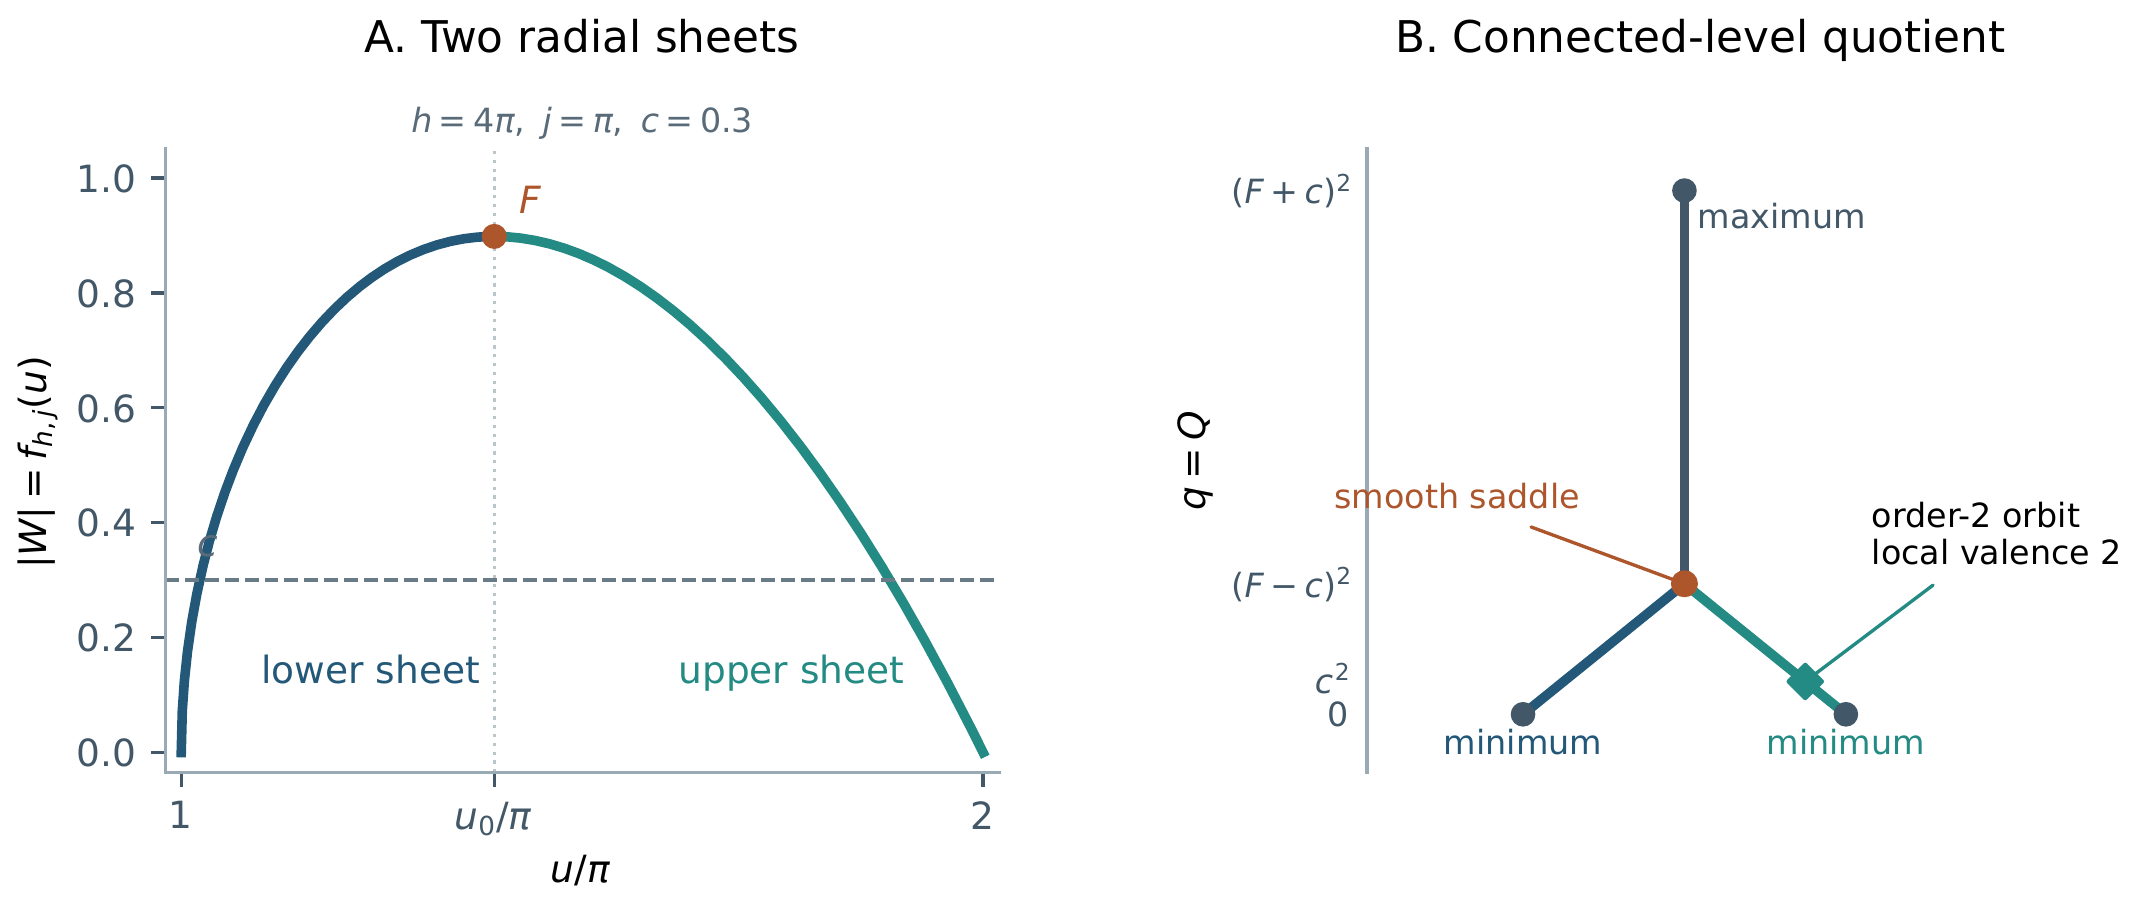
\includegraphics[width=\linewidth]{positive_winding_geometry.png}
\caption{$h=4\pi$, $j=\pi$, $c=0.3$ の例。左は二枚の radial sheets を与える
$f_{h,j}$、右は $Q$ の connected-level quotient である。
この例では $F>2c$ であり、$q=(F-c)^2$ の smooth saddle が真の三価分岐を生む。
$q=c^2$ の order-two orbit は上側の sheet にある singular orbit だが、
その局所 Reeb valence は2である。図の縦座標は実際の critical values を用いている。}
\label{pw:figure}
\end{figure}

上の generic reduction は $j\ne0$ を仮定したが、下 branch の focus fiber は
$x\ne0$ の exact coordinates で直接扱える。
\begin{equation}\label{pw:exact-axis}
 Y=e^{-4\pi i\theta_x}y,\qquad Z=z,
 \qquad
 \lambda=H\,d\theta_x+\rho_Yd\theta_Y+\rho_Zd\theta_Z.
\end{equation}
逆写像は
$x=\sqrt{(H-2\rho_Y)/\pi}\,e^{2\pi i\theta_x}$,
$y=e^{4\pi i\theta_x}Y$, $z=Z$ であり、domain は $H>2\rho_Y$ である。
従ってこれは genuine exact symplectic chart であり、
\begin{equation}\label{pw:axis-family}
 J=\rho_Y-\rho_Z,\qquad
 W=\frac{H-2\rho_Y}{\pi}\,YZ
\end{equation}
が厳密に成り立つ。

\begin{proposition}[分離された compact focus end]
\label{pw:focus}
$h>4\pi\sqrt c$ なら、$(H,J,Q)=(h,0,c^2)$ の fiber は二つの connected components を持つ。
下 branch の component は一つの rank-one focus--focus orbit を持つ
$S^1\times$(once-pinched torus) であり、上 branch の hyperbolic orbit と分離している。
$h$ をこの不等式を満たす compact interval 内で動かせば、
下 branch の全 compact fibers を含む focus curve block を、一様な小さい $(j,q)$-window 上に取れる。
\end{proposition}

\begin{proof}
$j=0$ では $u=\rho_Y=\rho_Z$ であり、
\[
 R=|W|=\frac{(h-2u)u}{\pi^2},\quad
 u_0=h/4,\quad F(h,0)=\frac{h^2}{8\pi^2}.
\]
下 branch の解は
\begin{equation}\label{pw:lower-root}
 u_-(h,R)=\frac{h-\sqrt{h^2-8\pi^2R}}4,
 \qquad 0\le R<F(h,0).
\end{equation}
Node を通る circle $|W-c|=c$ は $0\le R\le2c$ を満たす。
$h>4\pi\sqrt c$ はちょうど $F(h,0)>2c$ なので、
この circle 全体は disk の内部にあり、二つの radial branches の lifts は交わらない。
下 branch では $W=0$ において $Y=Z=0$ の一つの orbit だけが潰れ、
他の点では $J$-orbit は free circle である。
従って $H=h$ で reduction した四次元空間の $(J,Q)$-fiber は once-pinched torus である。
式\eqref{pw:exact-axis}により $\theta_x$ は独立な circle factor なので、元の fiber はその $S^1$ との積である。

原点での quadratic pair は
\[
 J=\pi(|Y|^2-|Z|^2),\qquad
 Q-c^2=-\frac{2ch}{\pi}\operatorname{Re}(YZ)+O(4)
\]
であり、nondegenerate focus--focus 型である。
上 branch の $W=0$ は $x=0$ に対応し、既述の hyperbolic orbit を持つ。
両者の間には $u=u_0$ の positive radial gap がある。
Compact な $h$-interval では $F(h,0)-2c$ が一様に正なので、
$j$ と $q-c^2$ を十分小さくしても二つの branches は分離したままである。
Properness と quotient の一意性により、この下 branch 全体が所要の compact block となる。
\end{proof}

Original disk frames における $x$-axis の mixed coefficient は $-2c\bar x^2$ なので、
削除 disk と逆向きの境界 winding は $+2$ である。
式\eqref{pw:exact-axis}の frame change は $x\ne0$ の annulus 上では well-defined だが、
$x=0$ の disk へは延びない。
従って命題\ref{pw:focus}は、所定の divisor-normal circle を disk まで保つ比較を主張していない。

\begin{corollary}[一次共役因子の smooth-reduction 模型]
\label{pw:m1}
$W_1=\bar x yz$, $H_1=\rho_x+\rho_y$, $J=\rho_y-\rho_z$,
$Q_1=|W_1-c|^2$ と置く。
$j\ne0$, $h>\max(0,j)$ の reduction は両極とも smooth な sphere であり、
$\phi_1=-\theta_x+\theta_y+\theta_z$ に対して $\omega_{\rm red}=du\wedge d\phi_1$ である。
Radial function と唯一の maximum point は
\[
 f_1(u)=\frac{\sqrt{(h-u)u(u-j)}}{\pi^{3/2}},\qquad
 u_1=\frac{h+j+\sqrt{h^2-hj+j^2}}3,
 \qquad \max(0,j)\le u\le h.
\]
$F_1=f_1(u_1)>c$ なら Reeb quotient は $Y$ 型であり、
$q_s=(F_1-c)^2$ の whole saddle fiber は $T^2\times(S^1\vee S^1)$ である。
ここでは $F_1=2c$ を除外する必要はない。
$F_1<c$ と $F_1=c$ の分類も定理\ref{pw:reeb}と同じである。

$j=0$ では
\[
 u_1=2h/3,\qquad F_1(h,0)=\frac{2h^{3/2}}{3\sqrt3\,\pi^{3/2}},
 \qquad F_1(h,0)>2c\ \Longleftrightarrow\ h>3\pi c^{2/3}.
\]
この範囲の $(h,0,c^2)$-fiber は、下側の
$S^1\times$(once-pinched torus) と上側の regular $T^3$ に分離する。
下 component は compact な $h$-interval 上で一様な focus block を与える。
各 nonzero axis の transverse 型は、$x$-axis が focus--focus、
$y,z$-axes が elliptic--elliptic である。
\end{corollary}

\begin{proof}
Weights $(1,0),(1,1),(0,-1)$ の任意の二つは unimodular なので、
$j\ne0$ の moment level では両極を含め action が free である。
また $(\log f_1)''<0$ で、critical equation は
$3u^2-2(h+j)u+hj=0$ となる。
命題\ref{pw:reduction}の double-disk argument と系\ref{pw:compact}の
graph 上の principal bundle の議論を適用できる。
上極では $W_1$ は非零定数倍の $\bar x$ を leading term とする smooth coordinate なので、
$Q_1=c^2$ も regular である。

$x\ne0$ では $Y=e^{-2\pi i\theta_x}y$, $Z=z$ によって厳密に
\[
 \lambda=H_1d\theta_x+\rho_Yd\theta_Y+\rho_Zd\theta_Z,
 \qquad W_1=\sqrt{\frac{H_1-\rho_Y}{\pi}}\,YZ
\]
となる。$j=0$ の lower branch は
$u^2(h-u)=\pi^3R^2$ の $0\le u<2h/3$ の解である。
$F_1>2c$ なら $|W_1-c|=c$ 全体がこの branch に入り、
命題\ref{pw:focus}と同じ積分解と uniform gap の議論が使える。
原点での $(J,Q_1-c^2)$ の quadratic pair は非零係数の $\operatorname{Re}(YZ)$ を持つ focus 型である。
一方、$y$-axis の stabilizer moment は $H_1-J=\rho_x+\rho_z$、
もう一方の quadratic は $-2c\operatorname{Re}(y_0\bar xz)$ である。
Unitary basis によってこの二つを $|v_1|^2,|v_2|^2$ の線形結合へ同時対角化でき、
elliptic--elliptic 型となる。$z$-axis も同様である。
\end{proof}

\begin{remark}[Semistable frames への位相変換]
\label{pw:semistable-phase}
本節の winding $+1,+2$ は original disk frames に関する値である。
第\ref{sc:phase}節の $C_{56}$ の端では、固定した $t\ne0$ に対し $y=tY/x$ なので、
mixed coefficient は
\[
 \gamma_{\rm ss}(x)=\frac{t}{x}\gamma_{\rm orig}(x),\qquad
 \operatorname{wind}_{\rm ss}=\operatorname{wind}_{\rm orig}+1
\]
と変換される。境界は常に削除 disk と逆向きである。
定数 $-2c$ を省略した係数を比較すると、次の表となる。
\[
\begin{array}{c|r|c|r}
 W&\text{original winding}&\gamma_{\rm ss}/(-2c)&\text{semistable winding}\\ \hline
 xyz&-1&t&0\\
 yz&0&t/x&1\\
 \bar xyz&1&t\bar x/x&2\\
 \bar x^2yz&2&t\bar x^2/x&3.
\end{array}
\]
従って系\ref{pw:m1}の模型が、第\ref{sc:phase}節の最大 winding を最小にする配分の
$+2$ の端に対応する候補となる。
$\bar x^2yz$ の模型の $+2$ を、その配分の $+2$ と直接同一視しない。
一方 $\sigma=L_1^3L_2L_3L_4$ を選べば semistable winding は $(3,1,1,1)$ となり、
$6(3+1+1+1)=36$ という別の位相収支も満たせる。

これらは固定した非零 $t$ の annulus 上の phase 計算である。
$t\to0$ で非零 Hessian を残すには、$W/t$ を使うなどの scale の選択を別途指定する必要がある。
またこの表は、actual Kähler form、normal circles、marked actions、whole fibers を保つ
relative symplectic identification を与えるものではない。
\end{remark}

この計算から得る具体的な次の課題は、下 branch の正の winding focus ends、
上 branch の有限 isotropy を持つ singular wall、内部の $Y$ 型 saddle を、
actual semistable geometry の中で相対的に配置することである。
有限 isotropy の wall と他の coordinate axes の退化は、二次共役因子 $\bar x^2yz$ の模型に属する。
その $F>2c$ の領域では focus component と上の singular wall を分離して扱える。
一次共役因子 $\bar xyz$ の模型では、上の component は regular であり、他の axes は elliptic--elliptic となる。
二次模型の $F=2c$ での collision、各模型の $F=c$ の degenerate minimum、
elliptic endpoints と残る axis singularities を含む全 corner の処理は未完了である。
本節は全 corner や boundary-free global fibration の完成ではなく、
compact fibers を保った正の winding と真の余次元1分岐が共存する finite-neck prototype を与える。


第\ref{tp:section}節では、この prototype を chosen graph Kähler form へ実際に移し、
中央の一端と exact に比較する。
第\ref{ai:section}節では、$x=0$ を除いても whole focus と true saddle が残る compact block を取り、
actual annulus へ入れる。従って prototype の位相計算から actual な局所構成へ進めるが、
除いた端と geometric corner 全体の充填は別の問題として残る。

\section{三変数積模型の axis end と compact nodal family の厳密な比較}
\label{ae:section}

本節の対象は、\emph{標準 symplectic form を持つ $\CC^3$ 上の模型}である。
この模型の一つの axis end を、compact fiber 全体を含めて二変数 nodal family に同定し、
さらにその端に厳密に一致する pants block を作る。
Actual な半安定 corner $xyz=tw$ の Kähler form と全 divisor framings を
この標準模型へ同時に同定することは、別の構成課題として残す。

以下、全ての角変数は周期1とし、$u\in\CC$ に対して
$\rho_u=\pi|u|^2$, $\theta_u=\arg u/(2\pi)$ と置く。
$\rho_u\,d\theta_u$ は $u=0$ を越して滑らかに延びる。
標準 primitive と symplectic form は
\[
 \lambda_3=\rho_xd\theta_x+\rho_yd\theta_y+\rho_zd\theta_z,
 \qquad \Omega_3=d\lambda_3
\]
である。$\varepsilon>0$ を固定し、三つの可換関数
\begin{equation}\label{ae:three-variable}
 F_1=\rho_x-\rho_y,\qquad F_2=\rho_x-\rho_z,
 \qquad Q=|xyz-\varepsilon|^2
\end{equation}
を考える。Hamiltonian vector field の規約は $\iota_{X_f}\Omega=-df$ である。

\subsection{Primitive を保つ action--angle 座標}

\begin{proposition}\label{ae:exact-coordinate}
$x\ne0$ 上で
\begin{equation}\label{ae:coordinate-formula}
 \theta=\theta_x,\qquad H=\rho_x-\rho_y,\qquad
 Y=e^{2\pi i\theta}y,\qquad Z=z
\end{equation}
と置く。
これは $x\ne0$ の領域を
\[
 \{(H,\theta,Y,Z)\in\RR\times S^1\times\CC^2:
 H+\pi|Y|^2>0\}
\]
へ写す exact symplectomorphism であり、primitive は実際に
\begin{equation}\label{ae:primitive-equality}
 \lambda_3=H\,d\theta+\pi|Y|^2d\theta_Y+\pi|Z|^2d\theta_Z
\end{equation}
と一致する。
$J=\pi(|Y|^2-|Z|^2)$, $t=\pi|Y|^2$ と書くと
\begin{equation}\label{ae:radial-family}
 F_1=H,\qquad F_2=H+J,\qquad
 Q_H(Y,Z)=\left|\sqrt{\frac{H+t}{\pi}}\,YZ-\varepsilon\right|^2.
\end{equation}
\end{proposition}

\begin{proof}
$\rho_Y=\rho_y$, $\rho_Z=\rho_z$ であり、
$d\theta_Y=d\theta+d\theta_y$ だから
\[
 \rho_xd\theta+\rho_yd\theta_y+\rho_zd\theta_z
 =(\rho_x-\rho_y)d\theta+\rho_Yd\theta_Y+\rho_Zd\theta_Z.
\]
これは exact form を加えることなく primitive 自体の等式である。
逆写像は
\[
 x=\sqrt{\frac{H+t}{\pi}}e^{2\pi i\theta},\qquad
 y=e^{-2\pi i\theta}Y,\qquad z=Z
\]
なので、所定の領域上で滑らかな同型となる。
この式を $xyz$ に代入すれば式\eqref{ae:radial-family}も得る。
\end{proof}

したがって位相因子 $e^{2\pi i\theta}$ は、longitudinal action を
$\rho_x$ から $H=\rho_x-\rho_y$ に変える exact shear により取り除ける。
一方、振幅 $|x|=\sqrt{(H+t)/\pi}$ は依然として $Q_H$ に残る。
式\eqref{ae:radial-family}は、固定した四次元 fibration と circle の単純な積ではなく、
$H$ に依存する compact nodal family である。

\subsection{Circle reduction と全 fiber の compact 性}

以後 $0<A<B$ を固定し、$H\in[A,B]$ の end を扱う。
$w=YZ$ とし、$J=j$ の上で
\begin{equation}\label{ae:W-coordinate}
 W=\sqrt{\frac{H+t}{\pi}}\,w
\end{equation}
と置く。

\begin{lemma}\label{ae:cubic}
固定した $H>0$, $j\in\RR$, $R=|W|\ge0$ に対し、$t$ は
\begin{equation}\label{ae:cubic-equation}
 t(t-j)(H+t)=\pi^3R^2,\qquad t\ge\max(j,0)
\end{equation}
の一意な解である。
$w\mapsto W$ は各 $j$ における radial homeomorphism であり、
quotient の原点 $(j,w)=(0,0)$ 以外では滑らかな局所座標変換である。
\end{lemma}

\begin{proof}
$\pi|Z|^2=t-j$ なので
$|w|^2=t(t-j)/\pi^2$ である。
これを式\eqref{ae:W-coordinate}に代入して cubic equation を得る。
左辺は $t=\max(j,0)$ で零となり、無限大へ発散する。
その微分は
\begin{equation}\label{ae:D}
 D=(2t-j)(H+t)+t(t-j)
\end{equation}
である。
$t\ge\max(j,0)$ では両項は非負であり、$(j,t)=(0,0)$ 以外では $D>0$ である。
これにより存在・一意性と単調性が従う。
$W$ の位相は $w$ と同じであり、その絶対値は $|w|$ の連続な狭義増加関数である。
Circle action の free locus では $(j,w)$ は滑らかな quotient coordinates なので、
上の微分の計算から最後の主張も従う。
\end{proof}

\begin{proposition}\label{ae:compact-end}
$a>0$, $0<\vartheta<1$ を固定し、$(j,q)=(0,\varepsilon^2)$ を内部に含む
小さい compact disk $U$ を
\begin{equation}\label{ae:end-window}
 |j|\le a\varepsilon,\qquad |q-\varepsilon^2|\le\vartheta\varepsilon^2
\end{equation}
の中に取る。
$(H,J,Q_H)$ の逆像
\[
 M_{A,B,U}=\{\,H\in[A,B],\ (J,Q_H)\in U\,\}
\]
は、$\theta$-circle を含めて compact な saturated end である。
正則 fiber は $T^3$、$(j,q)=(0,\varepsilon^2)$ の fiber は
$(\text{pinched }T^2)\times S^1$ である。
$\varepsilon$ を十分小さくすれば、この全 end は任意に指定した小さい normal disk と、
$[A,B]$ より少し広い $x$-axis annulus の中に入る。
\end{proposition}

\begin{proof}
固定した $(H,j,q)$ 上で $W$ は円 $|W-\varepsilon|=\sqrt q$ を動く。
補題\ref{ae:cubic}により、各 $W$ に対応する半径は一意である。
$J$ が生成する逆位相 circle action は $(Y,Z)=(0,0)$ 以外で自由であり、
その quotient は $(j,w)$、従って $(j,W)$ で記述される。
円が $(j,W)=(0,0)$ を通らない場合、normal fiber は円上の principal circle bundle、
従って $T^2$ である。
$j=0,q=\varepsilon^2$ では一つの orbit circle が潰れて once-pinched torus となる。
$Q_H=0$ の別の critical locus は式\eqref{ae:end-window}から除かれている。
$\theta$ は自由な circle coordinate なので、全 fiber の位相型が従う。

Compact 性のために、$C_\vartheta=1+\sqrt{1+\vartheta}$ と置くと
\[
 |W|\le C_\vartheta\varepsilon,\qquad
 |w|\le\sqrt{\frac\pi A}|W|
\]
である。また
\begin{equation}\label{ae:normal-radius}
 |Y|^2+|Z|^2
 =\sqrt{(j/\pi)^2+4|w|^2}
 \le\varepsilon\sqrt{(a/\pi)^2+4\pi C_\vartheta^2/A}.
\end{equation}
従って $0\le t\le K\varepsilon$ となる一様定数 $K$ がある。
$H$ と $\theta$ の領域も compact なので、閉集合 $M_{A,B,U}$ は compact となる。
原座標では
\begin{equation}\label{ae:x-radius}
 \rho_x=H+t\in[A,B+K\varepsilon].
\end{equation}
この評価と式\eqref{ae:normal-radius}が最後の主張を与える。
\end{proof}

\begin{remark}\label{ae:saturated-warning}
固定すべき action interval は $H\in[A,B]$ である。
$\rho_x=H+t$ は一つの normal torus 上で変動するので、
単に $\rho_x\in[A,B]$ として領域を切ると、一般には compact fibers を切断する。
また $A>0$ は本命題の仮定である。
$H=j=0$ では式\eqref{ae:cubic-equation}は $t=\pi R^{2/3}$ となり、
$x$-axis の通常の product normal approximation を corner 自身まで一様には延ばせない。
\end{remark}

\subsection{Normal scale と action・return holonomy}

固定軸 $(Y,Z)=(0,0)$ における Taylor 展開は
\begin{equation}\label{ae:hessian}
 Q_H-\varepsilon^2
 =-2\varepsilon\sqrt{H/\pi}\operatorname{Re}(YZ)
 +O\bigl(|(Y,Z)|^4\bigr)
\end{equation}
である。
振幅を固定軸上の値で凍結すれば
\begin{equation}\label{ae:frozen}
 Q_H^{\mathrm{fr}}=\frac H\pi|YZ-c_H|^2,
 \qquad c_H=\varepsilon\sqrt{\pi/H}
\end{equation}
となる。これは同じ normal Hessian を持つが、全 compact fiber の return data まで
一致するとは限らない。以下で実際に差を計算する。

\begin{proposition}\label{ae:action}
Regular values の単連結な小領域で complementary cycle を mark する。
その normal action は、適切な cycle chart で
\begin{equation}\label{ae:action-integral}
 I(H,j,q)=\frac1{2\pi}
 \int_{|W-\varepsilon|=\sqrt q}
 t_H(j,|W|)\,d\arg W
\end{equation}
と書ける。ここで $t_H$ は式\eqref{ae:cubic-equation}の解である。
Cycle chart を変えると $j$ の整数倍を加えることがある。
残り二つの action は $H$ と $j$ である。
したがって complementary cycle の period covector は $dI$ であり、
$H$-angle を閉じるための補正時間は $\partial_H I$ である。
\end{proposition}

\begin{proof}
Normal primitive は、$J=j$ の上で
\[
 \lambda_N=t\,d\theta_Y+(t-j)d\theta_Z
 =\frac{t}{2\pi}d\arg(YZ)-j\,d\theta_Z.
\]
$Z$ の位相を零にする局所切断では、$\arg(YZ)=\arg W$ だから
式\eqref{ae:action-integral}を得る。
別の切断は $J$-orbit を整数回加えることがあり、その action は $j$ である。
円が $W=0$ を通る正則値では、必要に応じて $Y$ を使う切断へ切り替える。
この場合は積分中の $t$ を $t-j$ に置き換え、上の整数倍の変更で滑らかに継続する。
したがって式は、origin を横切る極座標切断を無理に一つに固定する主張ではない。

$\theta$-orbit と $J$-orbit の primitive の積分はそれぞれ $H,j$ である。
一般に、mark した cycle に沿って Hamiltonian vector fields の組合せが
周期1の閉軌道を与え、その係数を $\tau_H,\tau_J,\tau_Q$ とすると、
cycle integral の微分は
\[
 dI=\tau_H\,dH+\tau_J\,dj+\tau_Q\,dq
\]
となる。
実際、cycle の変形 vector field を $V$ とすれば、Cartan formula により
その積分の微分は $\int\Omega(V,\dot\gamma)$ であり、
$\Omega(V,X_f)=df(V)$ を使えばこの等式を得る。
これが period covector の記述を与える。
\end{proof}

微分も cubic equation から直接求まる。
式\eqref{ae:D}の $D$ を用い、$R,j$ を固定して微分すれば
\begin{equation}\label{ae:implicit-derivatives}
 \partial_Ht=-\frac{t(t-j)}D,\qquad
 \partial_jt=\frac{t(H+t)}D,\qquad
 \partial_Rt=\frac{2\pi^3R}D.
\end{equation}
これにより $H$ とともに動く action family を、単なる leading term でなく正確に追える。

Product coordinates における $H$-circle bundle は、$d\theta$ を接続とすれば flat である。
しかし $X_{Q_H}$ の $\theta$ 方向の速度は $\partial_HQ_H$ である。
Normal return を $Q_H$-flow と必要な $J$-flow により行うとき、
その $H$-angle holonomy は
\begin{equation}\label{ae:holonomy}
 -\partial_H I\pmod{\ZZ}
\end{equation}
である。実際、これを閉じる $H$-flow の時間が $\partial_HI$ だからである。
従って circle bundle が位相的に自明で flat な接続を持つことと、
integrable system の return holonomy が零であることは異なる。

Focus--focus Taylor invariant を取り出すには、Eliasson coordinates に基底を規格化し、
action から universal logarithmic term を引く必要がある\cite{vungoc-local}。
生の $Q_H$ を規格化済みの座標とは扱わない。
式\eqref{ae:action-integral}は、その regularization の入力となる actual period family を与える。
本節の相対構成では、この family 自体を保つため、Taylor invariant の一致を
normal Hessian の一致から推測する必要はない。

\subsection{凍結した scale への exact 同定を妨げる action の差}

\begin{proposition}\label{ae:action-obstruction}
$H>0$ を固定し、$j=0$, $q=\varepsilon^2$ の compact nodal fiber を考える。
その非消失 cycle の標準 normal primitive に関する action を $A_H$ とする。
このとき
\begin{equation}\label{ae:action-strict}
 0<A_H<2\varepsilon\sqrt{\pi/H}=2c_H.
\end{equation}
右辺は式\eqref{ae:frozen}の凍結模型における、対応する nodal cycle の action である。
したがってこれら二つの reduced nodal neighborhoods の間に、
当該 cycle の marking と primitive を exact form を除いて保つ symplectomorphism は存在しない。
\end{proposition}

\begin{proof}
Nodal circle $|W-\varepsilon|=\varepsilon$ は、極座標で
\[
 R=2\varepsilon\cos\phi,\qquad -\pi/2\le\phi\le\pi/2
\]
と表せる。Origin における一つの orbit の collapse を含めても、
非消失 cycle の action は有限であり
\begin{equation}\label{ae:nodal-action}
 A_H=\frac1{2\pi}\int_{-\pi/2}^{\pi/2}
 t_H(0,2\varepsilon\cos\phi)\,d\phi
\end{equation}
となる。$j=0$ の cubic equation は
$t\sqrt{H+t}=\pi^{3/2}R$ と書ける。
従って $R>0$ では
\[
 0<t_H(0,R)<\frac{\pi^{3/2}R}{\sqrt H}.
\]
これを積分し、$\int_{-\pi/2}^{\pi/2}2\varepsilon\cos\phi\,d\phi=4\varepsilon$
を使えば式\eqref{ae:action-strict}を得る。

凍結模型では、$j=0$ の orbit quotient の normal action density は
$\pi|YZ|$ であり、nodal circle は $|YZ-c_H|=c_H$ である。
同じ極座標積分により action は $2c_H$ となる。
Exact symplectomorphism は mark した closed cycle の primitive integral を保つので、
上の厳密な不等式が矛盾を与える。
Cycle に vanishing cycle の整数倍を加えても、その nodal action は零だから差は消えない。
\end{proof}

固定した $H>0$ に対して、より詳しくは
\[
 t_H(0,R)=\frac{\pi^{3/2}}{\sqrt H}R
 -\frac{\pi^3}{2H^2}R^2+O(R^3)
\]
であり、式\eqref{ae:nodal-action}へ代入して
\begin{equation}\label{ae:action-expansion}
 A_H=2\varepsilon\sqrt{\pi/H}
 -\frac{\pi^3\varepsilon^2}{2H^2}+O(\varepsilon^3)
\end{equation}
を得る。$H$ が正の compact interval を動く場合、剰余も一様に取れる。

\begin{remark}\label{ae:obstruction-scope}
この action constant は、指定 primitive と cycle marking を保つ
\emph{exact} な比較の不変量である。
正規化された V\~u Ng\d{o}c の Taylor invariant そのものと同一視していない。
一般の非 exact な symplectic 同値を否定するものでもない。
また別の Auroux parameter を選べばこの一つの action を合わせられる可能性はあるが、
それだけで残りの return data の一致は従わない。
\end{remark}

\subsection{一つの axis end を保つ pants block の構成}

定数 scale の Auroux 模型へ置き換える代わりに、
式\eqref{ae:radial-family}の family をそのまま pants 上へ延ばす。
$(P,\omega_P)$ を symplectic pants とし、$h:P\to\RR$ を一つの saddle を持つ
Morse function とする。
Hermitian line bundles $E_+,E_-$ と unitary trivialization
$s:E_+\otimes E_-\simeq P\times\CC$ を選ぶ。
Dual connections を用い、前節と同じ coupling form
\[
 \Omega_P=p_P^*\omega_P+d(\rho_+\alpha_++\rho_-\alpha_-),
 \qquad J=\rho_+-\rho_-,\quad \rho_\pm=\pi|y_\pm|^2
\]
を入れる。
$a:P\to(0,\infty)$ を、$h$ の connected levels 上で一定な smooth basic function とし、
saddle の近傍では定数とする。
\begin{equation}\label{ae:pants-family}
 w=s(y\otimes z),\qquad
 Q_a=\left|\sqrt{\frac{a+\rho_+}{\pi}}\,w-\varepsilon\right|^2
\end{equation}
と置く。

\begin{theorem}\label{ae:one-end-pants}
十分小さい normal domain 上で $J,Q_a,h$ は Poisson commute する。
$\varepsilon$ と $(J,Q_a)$ の window を十分小さく選べば、
compact saturated pants block と、connected $h$-levels の Reeb quotient $r_h:P\to G_h$ を用いる写像
\[
 (J,Q_a,r_h):M\longrightarrow U\times G_h
\]
が得られ、その正則 fiber は $T^3$、
node と saddle の交点 fiber は
$(\text{pinched }T^2)\times\figeight$ となる。

一つの指定 boundary annulus に $(H,\theta)$ 座標があり、そこで
\[
 \omega_P=dH\wedge d\theta,\qquad h=H,\qquad a=H>0
\]
とする。さらに、その annulus 上で個別の unitary normal frames を指定し、
tensor trivialization はその積と一致するとする。
両 normal connections はこれらの frames に関して connection $1$-form が零となる
trivial flat connections に取る。このとき、その end は式\eqref{ae:three-variable}の $x$-axis end と、
\emph{whole compact fibers を含めて exact symplectomorphic} である。
他の二つの端のデータを自由に選ぶなら、これらの入力を pants 全体へ延ばせる。
\end{theorem}

\begin{proof}
Connection の水平・垂直分解で、$\rho_\pm$ と $w$ は水平輸送に関して一定である。
$Q_a$ の水平微分は $a$ によるものだけであり、$a$ が basic なので
$da(X_h)=0$ である。
水平 symplectic form は $\omega_P+J\kappa$ であり、曲面上ではこれは $\omega_P$ の
零でない関数倍だから、対応する $h$ の Hamiltonian direction も同じである。
従って $\{Q_a,h\}=0$ となる。
$J$ による circle action は $w,\rho_\pm$ を保つので $\{J,Q_a\}=0$ であり、
$\{J,h\}=0$ も成り立つ。

一つの connected $h$-level 上では $a$ は一定である。
従って補題\ref{ae:cubic}と命題\ref{ae:compact-end}の証明をそのまま使える。
$P$ は compact で $\min a>0$ なので半径評価も一様であり、compact saturated block を得る。
Regular level circle と critical figure-eight 上では normal circle bundle は位相的に自明である。
従って full fiber の位相は normal torus または pinched torus と、その level graph の積である。
その strata の水平射影は高々1次元、垂直部分は normal isotropic stratum であり、
mixed term はないので全 strata は isotropic である。
Saddle の近傍で $a$ は定数なので、同時特異点の二次部分は
focus--focus pair と Morse saddle の直和になる。

指定 annulus 上では coupling form が
$dH\wedge d\theta+\omega_{\CC^2}$ となり、$Q_a$ は $Q_H$ そのものである。
命題\ref{ae:exact-coordinate}の逆写像が、primitive と三つの関数を正確に同定する。
命題\ref{ae:compact-end}により、その写像は compact fibers 全体の上で定義される。
ここでは semiglobal な invariant を捨てず、actual radial family を保っている。

最後に、一つの boundary annulus に指定した line-bundle frame は、
他の二つの境界を自由にするなら pants 上へ延ばせる。
実際、$H^2(P;\ZZ)=0$ であり、制限写像
$H^1(P;\ZZ)\to H^1(S^1;\ZZ)$ は全射だから、
一つの境界における任意の winding を大域 gauge で実現できる。
この議論を二つの line に適用し、tensor trivialization も合わせて延ばす。
指定 trivial flat connections は接続の affine な接着によって延ばす。
$h$ は指定端を incoming または outgoing とする一つの saddle cobordism として延ばし、
他端の値を自由に選ぶ。
$a$ はその Reeb graph 上で正の関数として延ばし、vertex の近傍で正の定数とすればよい。
これらは全て指定端の小さい collar を変えずに行える。
\end{proof}

\begin{remark}\label{ae:one-end-limit}
この定理は、一つの標準 axis end を保ち、他の端を自由にする相対構成である。
全ての端を独立に指定する問題、actual $xyz=tw$ corner の Kähler form の比較、
および周囲の領域を充填して外側境界を消す問題は含まない。
別の actual symplectic neighborhood へこの pants block を移す際には、
指定 end first jets の大域 normal identification への延長と、
前節の相対 Moser の仮定を別途確認する必要がある。
\end{remark}

\subsection{位相・pole gauge の exact lift の範囲}

Annulus 上の unitary phase $e^{2\pi in\theta}$, $n\in\ZZ$ は、
\[
 (I,\theta,y,z)\longmapsto
 (I-n\rho_+,\theta,e^{2\pi in\theta}y,z)
\]
という exact lift を持つ。負の $n$ も許される。
Normal primitive に加わる $n\rho_+d\theta$ が longitudinal action の補正と相殺するためである。
固定した compact block に対しては、$|n|\rho_+$ が annulus の action 方向の余白より小さければよく、
式\eqref{ae:normal-radius}の評価により十分小さい $\varepsilon$ で実現できる。

しかし holomorphic gauge $x^n$ には、位相 $e^{2\pi in\theta}$ だけでなく振幅 $|x|^n$ もある。
上の shear はこの振幅を吸収しない。
例えば base angle を固定し、$y$ を文字通り $x^ny$ に変える写像は、
base を固定した normal tangent plane 上の symplectic area を $|x|^{2n}$ 倍する。
Longitudinal action だけの補正ではこの垂直方向の変化は相殺しない。
従って algebraic な pole 座標の変換だけから whole-fiber の symplectic 同定を結論できない。
また $n\ne0$ の位相 frame は $x=0$ を越して非消失に延びない。
Annulus 上で可能な exact lift と、corner を含む相対延長を区別する必要がある。

\section{正 winding の下 branch と異なる corner ends を結ぶ相対 pants}
\label{pe:section}

本節では一次共役因子 $\bar x yz$ の compact focus 成分を、
whole fibers と marked actions を保持したまま curve block の端へ接続する。
より一般に、標準積 $xyz$ の端と $\bar x yz$ の端という二つの指定端を
同じ pants block に一致させる。第三の端は自由に選ぶ。
これは標準 symplectic 模型での相対定理であり、actual corner に適用するときは、
その corner の形式から本節の形式への、whole fibers 上で定義された exact comparison を別途入力する。
全ての角変数の周期は1であり、$\rho_v=\pi|v|^2$ とする。

\subsection{減少する radial factor と一様な下 branch}

$H_-=\rho_x+\rho_y$, $J=\rho_y-\rho_z$,
$W_-=\bar x yz$, $Q_-=|W_--c|^2$ とする。
$x\ne0$ 上で
\[
 \theta=\theta_x,\quad Y=e^{-2\pi i\theta}y,\quad Z=z,
 \quad u=\rho_Y
\]
と置けば
\begin{equation}\label{pe:exact}
 \lambda_3=H_-d\theta+\rho_Yd\theta_Y+\rho_Zd\theta_Z,
 \qquad W_-=\sqrt{\frac{H_--u}{\pi}}YZ,
 \qquad H_->u.
\end{equation}
逆写像は
\[
 x=\sqrt{(H_--u)/\pi}\,e^{2\pi i\theta},\qquad
 y=e^{2\pi i\theta}Y,\quad z=Z
\]
であり、node $Y=Z=0$ でも滑らかである。
これは meridian frame の回転を longitudinal action の変更で補う厳密な恒等式であり、
normal coordinates だけを回転して base action を固定する操作ではない。

以下の補題は、減少・一定・増加する radial factor を一括して扱う。

\begin{lemma}[一様に分離された radial branch]\label{pe:uniform}
$0<A\le B$, $0<\delta<1/2$, $a_0>0$, $0<\vartheta<1$ を固定する。
$H\in[A,B]$, $s\in[-1,1]$ に対して
\[
 W_{H,s}=\sqrt{\frac{H+s u}{\pi}}YZ,
 \qquad J=\rho_Y-\rho_Z,
 \qquad Q_{H,s}=|W_{H,s}-c|^2
\]
と置き、$u\le\delta A$ の領域を考える。
十分小さい $c>0$ と、
\[
 |j|\le a_0c,\qquad |q-c^2|\le\vartheta c^2
\]
の中で $(0,c^2)$ を内部に持つ compact disk $U$ に対し、
\[
 \{H\in[A,B],\ (J,Q_{H,s})\in U,\ u\le\delta A\}
\]
は cutoff $u=\delta A$ と交わらず、全ての lower fibers を含む compact set である。
特に $s=-1$ ではこれは全三変数模型の下側の連結ファイバー成分を含む。
正則 normal fiber は $T^2$、$(j,q)=(0,c^2)$ の normal fiber は once-pinched torus である。
全ての主張と normal-radius estimate は $(H,s)$ に一様である。
\end{lemma}

\begin{proof}
$J=j$, $R=|W_{H,s}|$ 上の radial equation は
\begin{equation}\label{pe:root}
 u(u-j)(H+s u)=\pi^3R^2,\qquad u\ge L:=\max(0,j).
\end{equation}
左辺の $u$ 微分は
\begin{equation}\label{pe:D}
 D_{H,s}=(2u-j)(H+s u)+s u(u-j).
\end{equation}
$u\ge L$ なので $v=u-j\ge0$ であり、$D_{H,s}$ は $s$ に関して増加する。
$s=-1$ において
\[
 D_{H,-1}=(u+v)(H-u)-uv
         =u(H-u)+v(H-2u)>0
\]
が $(j,u)\ne(0,0)$ で成立する。ここでは $u\le\delta A<H/2$ を用いた。
従って全ての $s\in[-1,1]$ で、左辺は $[L,\delta A]$ 上で厳密に増加する。

$C_\vartheta=1+\sqrt{1+\vartheta}$ と置けば $R\le C_\vartheta c$ である。
$c$ を
\begin{equation}\label{pe:smallness}
 a_0c<\delta A/2,\qquad
 \pi^3 C_\vartheta^2c^2<\tfrac12\delta^2(1-\delta)A^3
\end{equation}
となるように選ぶ。
$u=\delta A$ で式\eqref{pe:root}の左辺は
\[
 \delta A(\delta A-j)(H+s\delta A)
 >\tfrac12\delta^2(1-\delta)A^3
\]
以上である。下端では零なので、各 $R\le C_\vartheta c$ に一意の解
$u=u_{H,s}(j,R)\in[L,\delta A)$ が存在する。
これにより cutoff は fiber と交わらず、$W$-circle 全体の lift が含まれる。

$H+s u\ge(1-\delta)A$ より
\[
 |YZ|\le\sqrt{\frac\pi{(1-\delta)A}}|W|,\qquad
 |Y|^2+|Z|^2
 \le c\sqrt{\left(\frac{a_0}\pi\right)^2+
                \frac{4\pi C_\vartheta^2}{(1-\delta)A}}.
\]
従って normal radius は $O(\sqrt c)$、$u$ は $O(c)$ であり、全 parameters に一様である。
元の負号模型では $\rho_x=H-u\in[A-Kc,B]$ なので、任意に指定した少し広い
$x$-axis annulus の中に全 fibers を入れられる。

$J$ の逆位相 circle は $(Y,Z)\ne(0,0)$ で自由であり、
各 $J$-quotient 上で $(j,W)$ は、原点以外において smooth coordinates である。
式\eqref{pe:D}が radial coordinate change の単調性を与える。
$|W-c|=\sqrt q$ の lift は通常は円上の principal circle bundle、
従って $T^2$ であり、$j=0,q=c^2$ では一つの orbit が潰れて pinched torus となる。
$Q=0$ は $q\ge(1-\vartheta)c^2>0$ により除外されている。
元の四次元 smooth coordinates で、node における二次部分は
\[
 J=\pi(|Y|^2-|Z|^2),\qquad
 Q_{H,s}-c^2=-2c\sqrt{H/\pi}\operatorname{Re}(YZ)+O(4),
\]
なので非退化 focus--focus 型である。
Quotient の root $u(j,R)$ が原点で smooth であるとは主張せず、
node の smoothness と非退化性はこの元の式で確認している。
\end{proof}

\begin{remark}[既に指定した $c$ に対する直接 barrier]
\label{pe:barrier}
条件\eqref{pe:smallness}は十分条件であり、最適ではない。
一般に $0<u_*<A/2$, $0\le j_0<u_*$ を選び、window 上の $|W|$ の上界 $R_*$ が
\[
 \pi^3R_*^2<u_*(u_*-j_0)(A-u_*)
\]
を満たせば、$|j|\le j_0$, $H\ge A$, $s\ge-1$ に対し cutoff $u=u_*$ は全 fibers と交わらない。
同じ derivative の証明が使え、primitive と return data に変更はない。
例えば chosen graph の中央 chamber から来る端で
$A>e_1$, $2c<f_A((A-e_1)/2)$ が既に成立していれば、
\[
 u_-(A,2c)<u_*<(A-e_1)/2<A/2
\]
を選ぶことができる。
$j_0$ と $Q$-window を十分小さくし、pants 全体で $a\ge A$ とすれば、
既に指定された $c$ を縮めずにこの一端を延長できる。
\end{remark}

\subsection{下 branch の full action と return holonomy}

$u_H^-(j,R)$ を $s=-1$ の解とする。Regular values の simply connected な cycle chart では、
normal primitive の complementary action は
\begin{equation}\label{pe:action}
 I_-(H,j,q)=\frac1{2\pi}
 \int_{|W-c|=\sqrt q}u_H^-(j,|W|)\,d\arg W
\end{equation}
である。$Z$ の位相を固定する section を用いた式であり、
section の変更は $j$ の整数倍を加える。
$W=0$ で $Z$ が消える regular level では $Y$ の section に切り替え、$u$ を $u-j$ に置き換える。
残り二つの actions は $H,j$ であり、full period covector は $dI_-$ である。
$Q$-flow と必要な $J$-flow による normal return の longitudinal holonomy は
\begin{equation}\label{pe:return}
 -\partial_H I_-\pmod{\ZZ}
\end{equation}
となる。これを閉じる $H$-flow の時間が $\partial_H I_-$ だからである。

式\eqref{pe:root}を微分すれば
\begin{equation}\label{pe:derivatives}
 \partial_Hu=-\frac{u(u-j)}{D_{H,-1}},\qquad
 \partial_ju=\frac{u(H-u)}{D_{H,-1}},\qquad
 \partial_Ru=\frac{2\pi^3R}{D_{H,-1}}
\end{equation}
を得る。従って return data は leading Hessian を凍結せず直接計算できる。

\begin{proposition}[正 winding end の nodal action]\label{pe:nodal}
$H>0$ を固定し、$0<c<H^{3/2}/(3\sqrt3\pi^{3/2})$ とする。
すなわち $H>3\pi c^{2/3}$ を仮定する。
Lower nodal fiber の非消失 cycle の action を $A_H^-(c)$ とすると
\begin{equation}\label{pe:nodal-integral}
 A_H^-(c)=\frac1{2\pi}\int_{-\pi/2}^{\pi/2}
 u_H^-(0,2c\cos\phi)\,d\phi
 >2c\sqrt{\pi/H}.
\end{equation}
さらに
\begin{equation}\label{pe:nodal-expansion}
 A_H^-(c)=2c\sqrt{\pi/H}
 +\frac{\pi^3c^2}{2H^2}
 +\frac{10\pi^{7/2}c^3}{3H^{7/2}}+O(c^4).
\end{equation}
$H$ が正の compact interval を動けば剰余は一様である。
\end{proposition}

\begin{proof}
$j=0$ で下 branch の方程式は
\[
 u\sqrt{H-u}=\pi^{3/2}R,\qquad 0\le u<2H/3
\]
である。$R>0$ では $\sqrt{H-u}<\sqrt H$ なので
$u>\pi^{3/2}R/\sqrt H$ となり、不等式が従う。
$u$ を $R$ の関数として $R=0$ の片側から展開すると
\[
 u=\frac{\pi^{3/2}}{\sqrt H}R
 +\frac{\pi^3}{2H^2}R^2
 +\frac{5\pi^{9/2}}{8H^{7/2}}R^3+O(R^4).
\]
$\int_{-\pi/2}^{\pi/2}\cos\phi\,d\phi=2$,
$\int\cos^2\phi\,d\phi=\pi/2$,
$\int\cos^3\phi\,d\phi=4/3$ を用いて式\eqref{pe:nodal-expansion}を得る。
なお $u(R)$ のこの片側展開は nodal action の計算用であり、
$R=|W|$ を smooth quotient coordinate とみなすものではない。
\end{proof}

係数を軸上の $\sqrt{H/\pi}$ に凍結した模型の nodal action は
$2c\sqrt{\pi/H}$ である。従って同じ primitive と cycle marking を
exact form を除いて保つ比較には、式\eqref{pe:nodal-integral}の差が障害となる。
増加する $xyz$ end の補正は $-\pi^3c^2/(2H^2)$ であり、今回の補正と逆符号である。
一般の unmarked、non-exact な symplectic 非同値や、正規化した focus Taylor invariant の
相違をこの一つの action だけから主張してはいけない。

\subsection{二つの指定端を exact に保つ hybrid pants}

$(P,\omega_P)$ を compact symplectic pair of pants とし、
$h:P\to\RR$ を一つの saddle を持ち境界近傍で regular な Morse function とする。
$E_+,E_-$ を Hermitian line bundles、
$\tau:E_+\otimes E_-\simeq P\times\CC$ を unitary tensor trivialization とする。
$\tau$ に関する dual connections を取り、
\[
 \Omega_P=p^*\omega_P+d(\rho_+\alpha_++\rho_-\alpha_-),
 \qquad J=\rho_+-\rho_-
\]
を考える。
$a:P\to(0,\infty)$ と $s:P\to[-1,1]$ は $h$ の connected levels 上で一定であり、
saddle の近傍では両方とも定数とする。
\begin{equation}\label{pe:hybrid}
 W_{a,s}=\sqrt{\frac{a+s\rho_+}{\pi}}\,\tau(y\otimes z),
 \qquad Q_{a,s}=|W_{a,s}-c|^2.
\end{equation}
十分小さい normal domain では radical は正である。

\begin{theorem}[二端相対構成]\label{pe:two-end}
上の入力に対して $J,Q_{a,s},h$ は Poisson commute する。
十分小さい共通 $c>0$ と補題\ref{pe:uniform}の window $U$ を選ぶと、
compact saturated block と、connected $h$-levels の Reeb quotient $r_h:P\to G_h$ を用いた
\[
 (J,Q_{a,s},r_h):M\longrightarrow U\times G_h
\]
が得られる。Regular fibers は $T^3$、node と saddle の同時 fiber は
$(\text{once-pinched }T^2)\times(S^1\vee S^1)$ であり、全ての fiber strata は isotropic である。

相異なる二つの boundary collars に symplectic coordinates
$(H_i,\theta_i)$ を指定し、$H_i$ は正の compact interval を動くとする。
そこで
\[
 \omega_P=dH_i\wedge d\theta_i,\qquad
 h=\chi_i(H_i),\qquad a=H_i,\qquad s=s_i\in\{-1,0,1\}
\]
とし、$\chi_i$ は strict monotone とする。
また個別の normal frames を指定し、その積を $\tau$ とし、
これらの frames に関する各 connection form を零にする。
このとき各 collar は、同じ $c$ と全 compact fibers を含めて、次の模型の axis end に
exact symplectomorphic である。
\begin{itemize}
 \item $s_i=-1$: $H_i=\rho_x+\rho_y$, $W=\bar x yz$ の下側 focus end。
 \item $s_i=+1$: $H_i=\rho_x-\rho_y$, $W=xyz$ の標準 focus end。
 \item $s_i=0$: $H_i=\rho_x$, $W=\sqrt{H_i/\pi}\,yz$ の無捩れ radial end。
\end{itemize}
写像は primitive と $(H_i,J,Q)$ を厳密に保つ。
$h$ のラベルは $h=\chi_i(H_i)$ により同定する。
第三の端を自由に選ぶなら、指定した二つの collars の全ての入力を pants 全体へ延長できる。
\end{theorem}

\begin{proof}
Horizontal transport は $\rho_\pm$ と $\tau(y\otimes z)$ を保つ。
$Q_{a,s}$ の horizontal derivative は $a,s$ によるものだけであり、
$da(X_h)=ds(X_h)=0$ なので $\{h,Q_{a,s}\}=0$ である。
Horizontal form は $\omega_P+J\kappa$ という曲面上の非退化2-form であり、
$h$ の Hamiltonian direction は $\omega_P$ のときと同じである。
$J$ の逆位相作用は各 $\rho_\pm$ と tensor product を保つので、残りの bracket も零である。

$A=\min a>0$, $B=\max a$ を用いて補題\ref{pe:uniform}を適用する。
$a,s$ は connected level ごとに一定なので、各 normal fiber 全体を同じ lower branch に取れる。
Normal cutoff は fiber と交わらず、compact base 上で全 block が compact である。
Regular circle と critical figure-eight 上の principal circle bundle は trivial なので、
normal torus または pinched torus と base level graph の積という位相型を得る。
各 stratum の horizontal dimension は高々1、vertical stratum は isotropic であり、
connection splitting に mixed symplectic term がないから、全 stratum は isotropic である。
Saddle 近傍で $a,s$ が定数なので、同時特異点の quadratic type は focus--focus と hyperbolic の直和となる。

指定 collar では normal connections が指定 frames に関して零なので、
$\Omega_P=dH_i\wedge d\theta_i+\omega_{\CC^2}$ となる。
$s_i=-1$ は式\eqref{pe:exact}、$s_i=+1$ は
$Y=e^{2\pi i\theta_i}y$, $\rho_x=H_i+\rho_Y$ による exact identity である。
$s_i=0$ は $x=\sqrt{H_i/\pi}e^{2\pi i\theta_i}$ により得られる。
補題\ref{pe:uniform}により写像は whole fibers 上で定義され、
式\eqref{pe:action}を含む全 return data が保たれる。

残るのは相対 extension である。
Pants の境界成分を二つ選んだ union を $A_{12}$ とすると、
\[
 H^2(P;\ZZ)=0,\qquad
 H^1(P;\ZZ)\longrightarrow H^1(A_{12};\ZZ)\simeq\ZZ^2
\]
の後者は同型である。従って各 line bundle を trivialize した後、
二つの指定 boundary frames の任意の winding を、ひとつの global gauge で同時に実現できる。
その homotopy class の一致を collar 上の exact phase correction により literal な一致へ直す。
これを $E_+,E_-$ に適用し、tensor trivialization も二つの collars を保って選ぶ。
指定零接続は、tensor trivialization に関して dual のまま affine に延長できる。

$h$ は三価 Morse cobordism として構成でき、$\chi_i$ を選ぶことで、
元の $H_i$ intervals が重なっていても異なる Reeb edges へ配置できる。
$a,s$ は graph 上で prescribed boundary functions を延ばし、
vertex の近くでは一定、かつ $a>0$, $|s|\le1$ とする。
第三の端の値はこの延長から選ぶ。

さらに $\omega_P$ の primitive $\beta$ を、二つの collars で
$\beta=H_i d\theta_i$ となるように選べる。
実際、任意の primitive とこれらの差は collar 上で closed であり、
上記 $H^1$ の同型でその periods を同時に補正し、残りの exact terms を cutoff して補正する。
従って
\[
 \lambda_P=p^*\beta+\rho_+\alpha_++\rho_-\alpha_-
\]
は指定した二つの collars で模型の primitive と文字通り一致する。
第三の境界の period は Stokes の公式により決まるため、独立に指定はしていない。
\end{proof}

\begin{corollary}[半安定 winding $2$ と $1$ を持つ二端]
\label{pe:central21}
第三端を自由にする二端相対構成において、一端では
$a=H$, $s=-1$、他端では $a=\pi$, $s=0$ としてよい。
前者は $(\rho_x+\rho_y,\rho_y-\rho_z,|\bar x yz-c|^2)$ の下側成分、
後者は $(\rho_x,\rho_y-\rho_z,|yz-c|^2)$ の全 compact focus end と
whole fibers および primitive を保って一致する。
Original disk frames の winding は順に $1,0$ であり、
半安定座標 $y=tY/x$ の下では $2,1$ となる。
\end{corollary}

\begin{proof}
定理の一般的な入力では $a$ は arbitrary positive basic function である。
後者の collar 上で $a=\pi$ と選べば $W_{a,0}=YZ$ であり、
$H=\rho_x$, $Y=y$, $Z=z$ により exact product coordinates を得る。
$c$ を両 ends の小ささ条件を満たすように取る。
$H$-label と $a$ が同じでなければならないのは、前者の radial factor を一致させる場合だけである。
Winding は mixed coefficient が original frames でそれぞれ $\bar x,1$ であることと、
半安定 frame への変換で $t/x$ が掛かることから従う。
\end{proof}

\begin{remark}[この構成が保つものと残すもの]\label{pe:scope}
正の winding は、$Y=e^{-2\pi i\theta}y$ の original disk frame に戻ると
mixed coefficient の phase $e^{-2\pi i\theta}$ として現れる。
標準積の端では逆の phase $e^{2\pi i\theta}$ が現れる。
Tensor frames を各 collar で選び直すことは finite annulus 上の exact shear に含まれるが、
それらが同じ中心 disk まで延長できるとは主張しない。

本定理は二つの指定端の primitive、actions、normal jets をその選んだ frames に関して保ち、
第三端を自由にする。
三端全ての独立指定、全 $C_{56}$ 上の prescribed disk framings、
actual global Kähler form との相対比較、$c\to0$ と $t\to0$ を同時に取る一様な domain、
人工境界の全消失は結論に含めない。
特に tensor winding の大域収支は別途満たさなければならず、
二つの自由な local corner phases を pants で接げることだけで全24端の問題は解けない。
\end{remark}

\section{例外曲線全体を通る surface bridge}
\label{exc:section}

第\ref{sc:phase}節の $S_{k5}$ 上では、曲線補正の端 $p_0$ と strict triple locus の点
$p_\infty$ は、一つの例外曲線の異なる点であった。
本節では、この例外曲線全体を含み、一方の点に compact focus fiber、
他方に elliptic boundary を持つ明示的な Lagrangian fibration を与える。
この種の blow-up fibration の存在は Auroux \cite[\S3.1.2]{auroux-blowup} の既知の模型である。
ここで必要なのは、その模型を半安定チャートの中で正規化し、
厳密な symplectic 座標、action、logarithmic residue と normal collar の変形を計算することである。

この節の構成は、まず一つの指定された K\"ahler 形式に対するものである。
任意に先に指定した compact focus germ と toric end の両方を、
それぞれの primitive と first jets まで保って比較する定理ではない。
その相対条件は末尾で分けて述べる。

\subsection{K\"ahler 形式と moment region}

\[
 M_e=\operatorname{Bl}_0\CC^2_{(z,w)},\qquad
 \pi:M_e\longrightarrow\CC^2,\qquad
 \operatorname{pr}:M_e\longrightarrow\PP^1
\]
と置く。$e>0$ は例外曲線 $E$ の \emph{symplectic area} であり、
ball radius や、その平方を表す記号ではない。
角変数は周期1とし、$\theta_u=\arg u/(2\pi)$、$\rho_u=\pi|u|^2$ とする。
\begin{equation}\label{exc:kahler}
 \omega_e=\pi^*\frac{i}{2}
       (dz\wedge d\bar z+dw\wedge d\bar w)
       +e\,\operatorname{pr}^*\omega_{\rm FS},
 \qquad \int_{\PP^1}\omega_{\rm FS}=1
\end{equation}
を用いる。Blow-down の pullback は $E$ の tangent direction のみで退化し、
第二項はその方向で正である。従って $\omega_e$ は $M_e$ 全体で K\"ahler であり、
$\int_E\omega_e=e$ となる。

二つのチャートを
\[
 (Y,z),\quad w=Yz;
 \qquad (U,w),\quad z=Uw;
 \qquad U=Y^{-1}
\]
と書く。$E$ はそれぞれ $z=0$, $w=0$ で表され、
\[
 p_0=(Y,z)=(0,0),\qquad
 p_\infty=(U,w)=(0,0),\qquad
 D=\widetilde{\{z=0\}}=\{U=0\}
\]
である。特に $D$ は $E$ と $p_\infty$ で交わり、$M_e\setminus D$ は
$(Y,z)$-chart 全体と一致する。

Blow-down の $z,w$ を別々に回転する torus の moment を
\begin{align}
 J&=\pi|z|^2+e\frac{|z|^2}{|z|^2+|w|^2},&
 K&=\pi|w|^2+e\frac{|w|^2}{|z|^2+|w|^2}
 \label{exc:toric-moments}
\end{align}
と正規化する。原点上の分数は $\PP^1$ 上の方向の関数として延長する。
Hamiltonian vector field の符号は $\iota_{X_H}\omega=-dH$ とするので、
$J$ は $z\mapsto e^{2\pi it}z$, $w\mapsto w$ という周期1の作用を生成する。
$(Y,z)$-chart では
\begin{equation}\label{exc:chart-moments}
 J=\pi|z|^2+\frac{e}{1+|Y|^2},\qquad
 K=\pi|Yz|^2+\frac{e|Y|^2}{1+|Y|^2}.
\end{equation}
Moment image は明示的に
\begin{equation}\label{exc:polytope}
 \Delta_e=\{(J,K):J\ge0,\ K\ge0,\ J+K\ge e\}
\end{equation}
である。実際、$J+K=e+\pi(|z|^2+|w|^2)$ であり、
$(J:K)=(|z|^2:|w|^2)$ だから、これらの不等式は必要十分である。
Facet $J=0$ は $D$、facet $J+K=e$ は $E$ に対応する。

\subsection{例外曲線を含む compact fibers}

$\varepsilon>0$ を固定し、
\begin{equation}\label{exc:fibration}
 W=\pi^*w,
 \qquad Q=|W-\varepsilon|^2,
 \qquad F_e=(J,Q):M_e\longrightarrow\RR^2
\end{equation}
と置く。$W$ は $J$ の circle action に不変なので、$\{J,Q\}=0$ である。

\begin{theorem}[例外曲線を通る明示的な fibration]
\label{exc:bridge}
任意の $\delta>0$ と $0<\eta<1$ に対し
\[
 B_{\delta,\eta}= [0,e+\delta]\times
   [(1-\eta)\varepsilon^2,(1+\eta)\varepsilon^2],
 \qquad \mathcal U_{\delta,\eta}=F_e^{-1}(B_{\delta,\eta})
\]
と置く。$\mathcal U_{\delta,\eta}$ は $E$ 全体を含む compact region であり、
$F_e$ の各 regular fiber は connected Lagrangian $T^2$ である。
その singular fibers は次の通りである。
\begin{enumerate}
\item $(J,Q)=(e,\varepsilon^2)$ の fiber は、一つの nondegenerate focus--focus point
 $p_0$ を持つ once-pinched torus である。
\item $J=0$ の fibers は $D$ 内の circles であり、rank-one elliptic 型である。
\end{enumerate}
この領域には他の singularities はない。
例外曲線の像は
\begin{equation}\label{exc:e-image}
 F_e(E)=[0,e]\times\{\varepsilon^2\},\qquad
 J|_E=\frac{e}{1+|Y|^2}.
\end{equation}
従ってこの一つの actual surface model が、$p_0$ の focus fiber と
$p_\infty$ の elliptic boundary を含む。
\end{theorem}

\begin{proof}
まず $J>0$ の quotient を直接記述する。
$R=|W|>0$、$u=|z|^2$ とすると、$J=s$ の条件は
\begin{equation}\label{exc:radial-equation}
 s=\pi u+\frac{eu}{u+R^2}
 \quad\Longleftrightarrow\quad
 \pi u^2+(\pi R^2+e-s)u-sR^2=0.
\end{equation}
左辺の最初の表示は $u\ge0$ に関して strictly increasing で、
$0$ から $+\infty$ まで動く。従って $s>0$ ごとに一つの正の解がある。
その点の $z$ の phase だけが自由であり、これは一つの free $J$-orbit である。
$W=0$ の場合は三つに分かれる。
\[
\begin{array}{c|c}
 s>e & Y=0,\quad \pi|z|^2=s-e,\\
 0<s<e & z=0,\quad |Y|^2=e/s-1,\\
 s=e & p_0.
\end{array}
\]
最初の二つはやはり free circles であり、最後だけが fixed point である。

$0<s<e$, $W=0$ の orbit では $Y\ne0$ なので $dW=Y\,dz$ が nonzero であり、
$dJ$ は $E$ 内の radial direction で nonzero である。
$s>e$, $W=0$ でも同様に $dW=z\,dY$ と $dJ$ は独立である。
$W\ne0$ では式\eqref{exc:radial-equation}の strict monotonicity が同じ独立性を与える。
従って $(J,W)$ は $J>0$ で $p_0$ を除いて circle quotient を滑らかに表示する。
$Q>0$ なら $W$-plane の $|W-\varepsilon|^2=Q$ は regular circle であるから、
その lift は principal circle bundle over a circle、すなわち $T^2$ である。
可換性と dimension によって Lagrangian となる。
Circle が $W=0$ を通り、かつ $s=e$ のときだけ、一つの orbit が点へ潰れる。
Cylinder の両端を同じ点へ潰した位相を持つので、fiber は once-pinched torus である。

$p_0$ で $u_0=\sqrt{e/\pi}\,Y$, $v_0=z$ と置くと、
$\omega_e(p_0)$ は $(u_0,v_0)$ の標準 symplectic form であり、二次項は
\begin{equation}\label{exc:focus-quadratic}
 J-e=\pi(|v_0|^2-|u_0|^2)+O(4),\qquad
 Q-\varepsilon^2=-2\varepsilon\sqrt{\pi/e}\,
      \operatorname{Re}(u_0v_0)+O(4).
\end{equation}
これは focus--focus Cartan の標準 pair の nonzero multiples である。
従って nondegenerate focus--focus point である。

一方、$(U,w)$-chart では
\begin{equation}\label{exc:boundary-moment}
 J=|U|^2\left(\pi|w|^2+\frac{e}{1+|U|^2}\right).
\end{equation}
$D=\{U=0\}$ における normal quadratic の係数は正であり、
$\omega_e|_D=\frac i2dw\wedge d\bar w$ である。
$Q>0$ の制限は $D$ 上の regular circle fibration なので、ここは rank-one elliptic 型となる。
特に $p_\infty$ においても $d(Q|_D)=-2\varepsilon\,d\operatorname{Re}w\ne0$ である。
$Q=0$ という別の elliptic locus は選んだ base window に含まれない。

最後に、$J\le e+\delta$ なら $\pi|z|^2\le e+\delta$、
有界な $Q$ なら $|w|$ も有界である。
Blow-up は $\CC^2\times\PP^1$ 内の closed submanifold なので、
$\mathcal U_{\delta,\eta}$ は compact である。
式\eqref{exc:e-image}は式\eqref{exc:chart-moments}から従う。
\end{proof}

\begin{remark}[縮小できる範囲]
\label{exc:shrink}
$e$ と $0<\eta<1$ を固定したまま $\varepsilon,\delta\to0$ とすれば、
$\mathcal U_{\delta,\eta}$ は任意に小さい $E$ の neighborhood に入る。
実際、$|w|\le(1+\sqrt{1+\eta})\varepsilon$ であり、
式\eqref{exc:radial-equation}の正の解は $J\le e+\delta$ の下で一様に $|z|\to0$ を満たす。
従って blow-down の像が原点へ縮み、その全逆像の極限は $E$ である。
これは、symplectic neighborhood の中に上の compact model を置く際に必要な縮小である。
\end{remark}

\subsection{Vanishing circle、normal weights と面積}

上の $J$-action の weights は
\begin{equation}\label{exc:weights}
 p_0:\quad(Y,z)\longmapsto
 (e^{-2\pi it}Y,e^{2\pi it}z),
 \qquad
 p_\infty:\quad(U,w)\longmapsto(e^{2\pi it}U,w)
\end{equation}
である。$p_0$ の vanishing cycle はこの primitive $J$-orbit であり、
$D$ 上で潰れる circle も同じ $J$-orbit である。
$M_e\setminus D$ の exact chart でこの orbit を $\alpha$ と向き付ければ、
その weights は $(+1,-1)$ で、$\int_\alpha\lambda_e=J-e$ となる。
$E$ の normal coordinates の transition は $w=Yz$ なので
\[
 N_{E/M_e}\simeq\mathcal O_{\PP^1}(-1).
\]
Normal weight は $p_0$ で $+1$、$p_\infty$ で $0$、
tangent weight はそれぞれ $-1,+1$ となる。

$0<s<e$ に対し、$E\cap\{J=s\}$ は $E$ を二つの symplectic discs に分ける。
その面積は
\begin{equation}\label{exc:cap-areas}
 \operatorname{Area}(\text{$p_0$ を含む cap})=e-s,
 \qquad
 \operatorname{Area}(\text{$p_\infty$ を含む cap})=s.
\end{equation}
実際、$p_0$ 側は $|Y|^2\le e/s-1$ であり、
$e\omega_{\rm FS}$ を積分すれば $e|Y|^2/(1+|Y|^2)=e-s$ を得る。
残りの面積は全体の $e$ から引けばよい。

$E$ の基底像を nodal-trade eigenray と同一視してはならない。
ここでは $E$ 上で circle moment $J$ 自身が変化し、
同じ circle が $p_0$ と boundary の両方で潰れる。
これは例外 sphere を備える blow-up model の記述である。
通常の node と elliptic edge の trade を適用するには、
そのための vanishing covector と collapsing covector の lattice 条件を別途満たす必要がある。

\subsection{例外曲線の punctured neighborhood の厳密 Darboux chart}

$(Y,z)$-chart 全体で、滑らかな primitive を
\begin{align}
 \lambda_e
 &=\rho_z\,d\theta_z+\rho_w\,d\theta_w
      +\frac{e|Y|^2}{1+|Y|^2}\,d\theta_Y \notag\\
 &=(J-e)\,d\theta_z+K\,d\theta_w
 \label{exc:primitive}
\end{align}
と取る。第一行の各 angular expression は、その radial coefficient により
対応する軸まで滑らかに延びる。第二行は torus locus での表示であり、
単独の $d\theta_z,d\theta_w$ の延長を主張していない。
直接微分すれば $d\lambda_e=\omega_e$ となる。

\begin{proposition}[Exact chart と reciprocal radial factor]
\label{exc:darboux}
\begin{equation}\label{exc:exact-coordinates}
 \xi=z\sqrt{1+|Y|^2},\qquad
 \zeta=Y\sqrt{J/\pi}
\end{equation}
は exact symplectomorphism
\[
 (M_e\setminus D,\lambda_e)\longrightarrow
 \bigl(\{\rho_\zeta<e+\rho_\xi\}\subset\CC^2,
       \rho_\xi\,d\theta_\xi+\rho_\zeta\,d\theta_\zeta\bigr)
\]
を与える。この chart では
\begin{align}
 J-e&=\rho_\xi-\rho_\zeta,
 &W&=\sqrt{\frac{\pi}{e+\rho_\xi}}\,\xi\zeta,\label{exc:inverse-radial}\\
 Q&=\left|\sqrt{\frac{\pi}{e+\rho_\xi}}\,\xi\zeta
                      -\varepsilon\right|^2.\notag
\end{align}
これは二次近似ではなく、当該 chart 全体での厳密な等式である。
\end{proposition}

\begin{proof}
\[
 a=J+K-e=\pi|z|^2(1+|Y|^2),\qquad b=K
\]
と置くと、$J=e+a-b>0$ であり、式\eqref{exc:exact-coordinates}から
$\rho_\xi=a$, $\rho_\zeta=b$ を得る。
また $\theta_\xi=\theta_z$, $\theta_\zeta=\theta_Y$、
$\theta_w=\theta_z+\theta_Y$ なので
\[
 \lambda_e=(J+K-e)d\theta_z+K\,d\theta_Y
           =a\,d\theta_\xi+b\,d\theta_\zeta.
\]
この計算は dense torus locus で成り立ち、両辺が滑らかなため chart 全体へ延びる。
逆写像は
\begin{equation}\label{exc:exact-inverse}
 J=e+\rho_\xi-\rho_\zeta,\qquad
 Y=\zeta\sqrt{\pi/J},\qquad
 z=\xi\sqrt{J/(e+\rho_\xi)}
\end{equation}
であり、指定した domain で滑らかである。
これにより global diffeomorphism と primitive の厳密な保存が分かる。
最後に $W=Yz$ に逆写像を代入すれば式\eqref{exc:inverse-radial}を得る。
\end{proof}

特に本節の compact focus germ は、第\ref{ae:section}節の一定 scale の germ に
単に置き換わるわけではない。
ここでは radial factor が $(e+\rho_\xi)^{-1/2}$ を含み、
その非線形部分は次の semiglobal action に現れる。

\subsection{Nodal action の正の二次補正}

$j=J-e$ とし、$a=\rho_\xi$, $b=\rho_\zeta=a-j$ とする。
式\eqref{exc:inverse-radial}より、$R=|W|$ は
\begin{equation}\label{exc:action-root-equation}
 a(a-j)=\pi R^2(e+a),\qquad a\ge\max(j,0),\qquad j>-e
\end{equation}
を満たす。$R>0$ に対する唯一の正の解は
\begin{equation}\label{exc:action-root}
 a_e(j,R)=\frac{j+\pi R^2+
     \sqrt{(j+\pi R^2)^2+4\pi eR^2}}2.
\end{equation}
$R=0$ では連続的に $a_e(j,0)=\max(j,0)$ とする。
この解は式\eqref{exc:action-root-equation}の条件を満たし、
元の quotient の一意性とも一致する。

例えば $\zeta$ の phase を固定できる cycle chart では、complementary action は
\begin{equation}\label{exc:action-integral}
 I_e(j,q)=\frac1{2\pi}
       \oint_{|W-\varepsilon|=\sqrt q}a_e(j,|W|)\,d\arg W
\end{equation}
で与えられる。別の lift を選ぶと $j$ の整数倍が加わり得る。
$j>0$, $W=0$ を跨ぐ chart では固定する phase を替える必要があり、
式\eqref{exc:action-integral}を全ての base point で単一の smooth action として使わない。
Node $j=0,q=\varepsilon^2$ での limiting action には、この整数倍の曖昧さは残らない。

\begin{proposition}[Marked nodal action]
\label{exc:nodal-action}
$\lambda_e$ と上の complementary cycle の極限を用いた nodal action を $A_e$ とする。
すると
\begin{align}
 A_e
 &=\frac{\pi}{2}\varepsilon^2
   +\varepsilon\sqrt{\frac e\pi}
   +\left(\frac e\pi+\varepsilon^2\right)
       \arctan\left(\varepsilon\sqrt{\frac\pi e}\right),
       \label{exc:action-closed}\\
 &=2\varepsilon\sqrt{\frac e\pi}
     +\frac\pi2\varepsilon^2+O(\varepsilon^3)
       \qquad(\varepsilon\to0,\ e\text{ fixed}).\label{exc:action-expansion}
\end{align}
さらに全ての $\varepsilon>0$ に対して
\begin{equation}\label{exc:action-positive}
 A_e>2\varepsilon\sqrt{e/\pi}+\frac\pi2\varepsilon^2.
\end{equation}
従って、radial factor をその原点での値 $\sqrt{\pi/e}$ に凍結した模型とは、
同じ $\varepsilon,e$、同じ primitive と marked cycle の下で nodal action が異なる。
\end{proposition}

\begin{proof}
$j=0$ では式\eqref{exc:action-root}が
\[
 a_e(0,R)=\frac\pi2R^2+
   \sqrt{\pi e}\,R\sqrt{1+\frac{\pi R^2}{4e}}
\]
となる。Node を通る circle $|W-\varepsilon|=\varepsilon$ は
\[
 W=R e^{i\phi},\quad R=2\varepsilon\cos\phi,
 \quad-\pi/2\le\phi\le\pi/2
\]
と書ける。両端は $W=0$ であり、この積分は regular cycles の極限として収束する。
従って
\[
 A_e=\frac\pi2\varepsilon^2+
 \varepsilon\sqrt{e/\pi}
 \int_{-\pi/2}^{\pi/2}\cos\phi
   \sqrt{1+\frac{\pi\varepsilon^2}{e}\cos^2\phi}\,d\phi.
\]
$v=\sin\phi$, $c=\pi\varepsilon^2/e$ と置けば残りの積分は
\[
 \int_{-1}^{1}\sqrt{1+c-cv^2}\,dv
       =1+\frac{1+c}{\sqrt c}\arctan\sqrt c
\]
となる。これを代入して式\eqref{exc:action-closed}を得る。
Taylor expansion により式\eqref{exc:action-expansion}が従う。
また $c>0$ のとき積分の integrand は $\cos\phi$ より内部で strictly larger なので、
その積分は $2$ より大きい。これが式\eqref{exc:action-positive}である。

凍結した模型では $a=\sqrt{\pi e}\,R$ なので、同じ積分は
$2\varepsilon\sqrt{e/\pi}$ となる。
Exact comparison が primitive と marked cycle を保てば、その積分も保存するから、
上の差はその比較への障害である。
\end{proof}

この命題は、全ての base reparametrizations や closed-form shifts を許した
unmarked symplectic equivalence の非存在を主張しない。
また、$\varepsilon$ を変更して一つの action を合わせても、
compact focus neighborhood の semiglobal invariant 全体が一致したことにはならない。
本節の inverse radial family をそのまま端の family として選べば、
不要な凍結によるこの比較問題を持ち込まずに済む。

\subsection{Strict triple divisor に沿う residue と全 $E$ の制約}

\begin{proposition}[Forced residue]
\label{exc:residue}
式\eqref{exc:primitive}の primitive は $D$ に沿って residue $-e$ を持つ。
より具体的には、$(U,w)$-chart の $U\ne0$ で
\begin{equation}\label{exc:residue-formula}
 \lambda_e=(J-e)d\theta_U+
              \pi(|z|^2+|w|^2)d\theta_w,
\end{equation}
であり、$\lambda_e+e\,d\theta_U$ はこの chart 全体へ滑らかに延びる。
この residue は、$M_e\setminus D$ 上で primitive を exact form だけ変更しても、
消去できない。
\end{proposition}

\begin{proof}
$\theta_z=\theta_U+\theta_w$ と $J+K-e=\pi(|z|^2+|w|^2)$ を
式\eqref{exc:primitive}へ代入する。
$J$ は式\eqref{exc:boundary-moment}の通り $|U|^2$ を因子に持つので、
$Jd\theta_U$ は滑らかである。
第二項も $z=Uw$ より $\pi|w|^2(1+|U|^2)d\theta_w$ であり滑らかである。
従って meridian を正向きに回る積分の極限は $-e$ である。
Exact form の閉曲線上の積分は零なので、この値は変わらない。

同じ結論は $E$ への Stokes の公式からも分かる。
$p_\infty$ の小さい disk を取り除いた $E$ の境界は、$U$ の positive meridian と逆向きである。
その境界上の積分は極限で $e$ となり、$\int_E\omega_e=e$ と一致する。
\end{proof}

\begin{proposition}[全例外曲線に対する一方向の obstruction]
\label{exc:whole-e}
半安定模型の $S_{k5}$ における二つの component-normal lines は、$E$ 上で
\begin{equation}\label{exc:component-degrees}
 \deg(N_{S_{k5}/D_5}|_E)=0,\qquad
 \deg(N_{S_{k5}/D_k}|_E)=-1.
\end{equation}
特に第一の line の connection curvature を $\kappa_x$、$w_x>0$ とすると、
$E$ 全体を含む neighborhood 上に smooth form $\beta$ で
\begin{equation}\label{exc:impossible-balance}
 d\beta=\omega_e+w_x\kappa_x
\end{equation}
を満たすものは存在しない。
従って、第\ref{mc:main}節の one-normal straightening の仮定を、
この normal line 一つだけで全 $E$ に拡張することはできない。
\end{proposition}

\begin{proof}
半安定チャートは $(x,T,Y,z)$, $w=Yz$, $f=xT$ と、
$(x,y,U,w)$, $z=Uw$, $f=xyU$ であり、重なりでは $y=YT$ である。
$D_5$ 内の $S_{k5}$ の normal coordinate は両方の chart で $x$ なので、その line は $E$ 上で trivial である。
$D_k$ 内の normal coordinates は $T,y$ であり、transition は $y=YT$ である。
これは $E$ の normal line と同じ $\mathcal O(-1)$ の transition である。
よって式\eqref{exc:component-degrees}を得る。
なお strict triple divisor は $E$ と一点で交わるので、normal degrees の和とその交点数は
$0-1+1=0$ となり、SNC relation と整合する。

式\eqref{exc:impossible-balance}を $E$ 上で積分すれば、左辺は零、右辺は
$e+w_x\int_E\kappa_x=e>0$ となり矛盾する。
第一の normal degree が零なので、curvature と $c_1$ の符号規約には依存しない。
\end{proof}

この obstruction は $M_e\setminus D$ 上の one-normal collar を排除しない。
そこでは $\kappa_x=0$, $\beta=\lambda_e$ と取れる。
しかし $D$ を戻した際に、命題\ref{exc:residue}の residue と
命題\ref{exc:whole-e}の degree を無視することはできない。
例外曲線全体を扱うには、他の normal directions と corner data の収支を同時に扱う必要がある。
正の weight を持つ normal direction を追加すれば自動的に balance する、という意味ではない。
Curvature の符号と residue を含む収支は命題\ref{ct:degree-residue}を参照されたい。

\subsection{Strict one-normal comparison の slanted face}

次の計算は、full corner が必要になる位置を座標として示す。
Flat $x$-normal bundle 上で normal moment を $\mu=\pi|x|^2$ とし、
\begin{align*}
 \lambda&=(\mu-w_x)d\theta_x+\lambda_e,\\
 \alpha_*&=d\theta_x-\lambda_e/w_x,
 &\lambda_*&=(\mu-w_x)\alpha_*
            =(\mu-w_x)d\theta_x+r\lambda_e,
 &r&=1-\mu/w_x>0
\end{align*}
と置く。これは第\ref{mc:single}節と同じ original/straightened の向きである。

\begin{proposition}[Strict comparison と facet の傾き]
\label{exc:slant}
Actual coordinates から straightened coordinates への strict map
$\Phi^*\lambda_*=\lambda$ は、$\mu,\theta_x$ と toric angles を保ち、
\begin{equation}\label{exc:slant-map}
 J_*=e+\frac{J-e}{r}
       =\frac{J-e\mu/w_x}{r},\qquad
 K_*=\frac K r
\end{equation}
と表される。従って target elliptic facet $J_*=0$ の pullback は
\begin{equation}\label{exc:slant-face}
 J=e\mu/w_x
\end{equation}
であり、actual divisor の facet $J=0$ とは $\mu>0$ で異なる。
逆写像の表式は $J=rJ_*+e\mu/w_x$ である。

Map が $M_e\setminus D$ 内に留まる domain は $J>e\mu/w_x$ である。
従ってこの比較は、そのまま actual $J=0$ face にまで延長する collar を与えない。
\end{proposition}

\begin{proof}
命題\ref{exc:darboux}の exact coordinates で
\[
 (\xi,\zeta)\longmapsto(\xi/\sqrt r,\zeta/\sqrt r)
\]
と取る。この map は角変数を保ち、$a=\rho_\xi,b=\rho_\zeta$ をそれぞれ $a/r,b/r$ へ送る。
従って pullback は $\Phi^*\lambda_e=\lambda_e/r$ であり、
上の $\lambda_*$ の表示から $\Phi^*\lambda_*=\lambda$ が厳密に成り立つ。
また $J=e+a-b$, $K=b$ なので式\eqref{exc:slant-map}を得る。
Target exact chart の不等式 $b/r<e+a/r$ は $J>e(1-r)=e\mu/w_x$ と同値である。
その境界が式\eqref{exc:slant-face}である。

同じ計算を Liouville field で書けば
\[
 Z_e=(J-e)\partial_J+K\partial_K,
 \qquad \iota_{Z_e}\omega_e=\lambda_e,
\]
の時間 $-\log r$ の flow である。
この field は $(Y,z)$-chart、すなわち exact chart では滑らかであるが、
residue のある $D$ を越えては同じ形で用いられない。
\end{proof}

式\eqref{exc:slant-face}は一つの選択した strict comparison の帰結であり、
一般の corner fibration の非存在を意味しない。
ただし、flat normal collar の formula を使ったまま $J_*=0$ と actual $J=0$ を同一視することはできない。
Normal moment、divisor face、primitive の三つを比較する際には、この shift を含める必要がある。

\subsection{Actual surface への比較と相対的な適用範囲}

\begin{corollary}[Graph K\"ahler form に対する actual restriction]
\label{exc:actual-graph}
半安定解消の graph K\"ahler form を第\ref{tc:surface}節のように選び、
第二の projective factor の面積係数を $e$ とすれば、
$S_{k5}$ の当該 neighborhood への制限は式\eqref{exc:kahler}と一致する。
従ってその選択に対して、定理\ref{exc:bridge}は actual central surface 上の明示的な fibration である。
\end{corollary}

\begin{proof}
$S_{k5}$ では $x=y=0$, $w=Yz$ である。
第一の projective coordinate $[x:t]=[1:T]$ は $[1:0]$ に固定され、
第二の $[xy:t]=[y:T]$ は $[Y:1]$ となる。
従って ambient Euclidean form の制限は $\omega_z+\omega_w$、
projective terms の制限は $e\omega_{\rm FS}[Y:1]$ であり、所要の式となる。
\end{proof}

他方、任意に与えられた actual symplectic form $\Omega$ と、
元の代数的な $E,D$ の両方を固定して、この模型へ移す主張には注意が必要である。
模型では $E,D$ は $p_\infty$ で symplectically orthogonal である。
Pair を両方送る symplectomorphism はこの直交性を保存するので、
actual pair が直交していなければ、そのままではそのような map は存在しない。

Existence のために $E$ を補助的な symplectic sphere として動かせ、
$E,D$ が正に横断交差する場合には、
$D$ を固定して $p_\infty$ の小さい neighborhood 内で $E$ を直交化できる。
その precise local statement は Evans \cite[\S5.2.1, Lemma 27]{evans-gompf} にある
Gompf isotopy である。すなわち、zero section と fibers が直交する symplectic disc bundle の中で、
zero section と一点で正に横断交差する symplectic surface を、交点近傍外では動かさず、
その点の normal fiber と一致するように isotopy できる。
ここでは zero section を $D$ として用いるので、$p_0$ とその近傍は動かさずに済む。
これは一方の surface を動かす isotopy であり、元の pair を固定した ambient symplectomorphism ではない。

直交化後、sphere の面積を $e=\int_E\Omega$ として合わせ、
normal degree $-1$ と交点の plumbing chart を合わせれば、
symplectic neighborhood theorem と relative Moser によって pair の小さい neighborhoods を同定できる
\cite[\S\S7.3,9.2]{cds-local}。
具体的には、sphere 上の area forms を全 area を保って合わせ、
normal symplectic line bundles を同定し、交点の小さい開近傍では
二つの方向を保つ symplectic plumbing identification を先に合わせる。
その first-jet identification を延長した map の pullback form と模型の form は、
zero section 上で full bilinear forms として一致する。
Radial homotopy で得る primitive を用いた Moser field は zero section 上で零となる。
Plumbing identification が既に一致する交点近傍では primitive も零に選べるので、
その部分を固定したまま、十分小さい neighborhood で symplectic identification を与える。
指定した end germs 上で initial identification が既に一致している場合だけ、その部分を固定して同じ議論ができる。
注意\ref{exc:shrink}により、小さい $\varepsilon,\delta$ を選べば compact bridge をこの neighborhood 内に入れられる。

従って、自由に local fibration を選ぶ surface-level existence と、
既に選んだ二つの end fibrations を相対的に接ぐ問題は区別される。
後者には少なくとも、compact focus fiber の semiglobal data、
primitive の marked periods、normal bundle と first jets、
$D$ に沿う residue の整合を確認する必要がある。
点での focus quadratic の一致だけでは、命題\ref{exc:nodal-action}の action 差さえ検出できない。

既知の surgery theorem の相対性も、この区別を省略しない。
Symington の nodal trade \cite[\S6, Lemma 6.3, Theorem 6.5]{symington} は、
node から edge への適切な embedded eigenray、途中の他の nodes の不存在、
vanishing/collapsing covectors の lattice-basis 条件の下で局所手術を比較する。
これは任意に指定した二つの end germs を同一視する定理ではない。
Chakravarthy--Groman \cite[Theorem 1.1, Definitions 2.2--2.3]{cg-at-blowup} の
almost-toric blow-up と symplectic blow-up の比較は、
affine-convex region とその surgery triangle、region の相対内部に収まる ball embedding を仮定し、
region 外で恒等な symplectomorphism を与える。
Divisor を保つ結論には ball/divisor compatibility が加わる。
具体的には、ball embedding が少し大きい ball に延長し、
そこで divisor との交わりが coordinate complex plane の像となることを要求する。
Blow-down 側では、exceptional sphere の toric $\mathcal O(-1)$ neighborhood 内で
divisor が一つの normal fiber に対応することが compatibility である。
本節ではこれらを存在引用の代用とせず、式\eqref{exc:kahler}--\eqref{exc:fibration}から fibers を直接構成した。

本節により、例外曲線を横断する二つの surface ends を同一の明示模型で持つ段階は成立する。
六次元の corner-to-curve gluing へ進むには、
その模型を actual normal directions に持ち上げ、
命題\ref{exc:whole-e}の degree と命題\ref{exc:slant}の moving facet を含む比較を行う必要がある。
全ての artificial boundary の消失は、この surface-level statement からは従わない。

\section{解消族を通じた一つの Kähler corner 模型}
\label{tc:section}

第\ref{sc:phase}節の半安定チャートと第\ref{exc:section}節の曲面模型を、
一つの明示的な Kähler form の中で実現する。
Hamiltonian torus の moment と不変な複素関数を組み合わせる手法自体は、
Gross \cite[\S\S1--2]{gross-toric}、Auroux \cite[\S3.3.1]{auroux-blowup}、
Casta\~no-Bernard--Matessi \cite[\S\S3.4,5.1]{cbm-conifold} の既知の構成に属する。
ここで必要なのは、今回の ordered resolution、二つの exceptional areas、
中心成分上の exceptional sphere、非零ファイバーの moments を同じ式で追うことである。
所定の全 boundary data を保つ任意の global Kähler form との比較までは主張しない。

\subsection{二つの射影直線への graph closure}

$V=\{xyz=tw\}\subset\CC^5$ とする。
有理写像 $[x:t]$, $[xy:t]$ の graph closure を $\widetilde V$ と書く。
二つの homogeneous coordinates を $[a:b]$, $[c:d]$ とすると、その方程式は
\begin{equation}\label{tc:incidence}
 xb=ta,\qquad bc=ay\,d,\qquad cz=dw.
\end{equation}

\begin{proposition}\label{tc:resolution}
$\widetilde V$ は滑らかな複素四次元多様体であり、$V$ への proper birational map を持つ。
$t:\widetilde V\to\CC$ は第\ref{sc:phase}節の ordered semistable resolution と同じである。
具体的には次の三つの affine charts で覆われる。
\[
\begin{array}{c|c|c}
\text{chart}&\text{coordinates}&\text{relations}\\ \hline
 b\ne0 &(t,X,y,z)&x=tX,\quad w=Xyz\\
 a,d\ne0 &(x,T,Y,z)&t=xT,\quad y=TY,\quad w=Yz\\
 a,c\ne0 &(x,y,U,w)&t=xyU,\quad z=Uw.
\end{array}
\]
原点上の exceptional fiber は二本の射影直線 $\ell_1\cup\ell_2$ であり、
二つの projection line bundles のそれぞれの次数は
\[
\begin{array}{c|cc}
 &\ell_1&\ell_2\\ \hline
 \mathrm{pr}_1^*\mathcal O(1)&1&0\\
 \mathrm{pr}_2^*\mathcal O(1)&0&1.
\end{array}
\]
\end{proposition}

\begin{proof}
$b=1$ とすると、第2式から $d\ne0$ である。
$d=1,a=X$ と置けば $c=Xy$ となり、最初の chart を得る。
$a=d=1,b=T,c=Y$ と置くと第二の chart を得る。
$a=c=1,d=U$ と置くと $b=yU$ となり、第三の chart を得る。
$b=0$ なら $a\ne0$ なので、残る二つの charts がその部分を覆う。
各 chart は $\CC^4$ であり、もとの有理写像の graph と稠密開集合で一致する。
従って式\eqref{tc:incidence}は余分な成分を持たず、graph closure を定める。
Projection は projective なので proper である。

第二の chart で、原点上の fiber は
$\{x=z=Y=0\}$ と $\{x=z=T=0\}$ の和である。
前者では $[a:b]=[1:T]$ のみ、後者では $[c:d]=[Y:1]$ のみが動く。
両者を隣の charts で閉じれば主張する二本の $\PP^1$ と次数表を得る。
\end{proof}

$\int_{\PP^1}\omega_{\mathrm{FS}}=1$ とし、$e_1,e_2>0$ に対し
\begin{equation}\label{tc:kahler}
 \widetilde\Omega
 =\omega_{\CC^5}
   +e_1\mathrm{pr}_1^*\omega_{\mathrm{FS}}
   +e_2\mathrm{pr}_2^*\omega_{\mathrm{FS}}
 \quad\text{on }\widetilde V
\end{equation}
と置く。これは product Kähler form の埋め込みによる制限なので Kähler である。
また $\int_{\ell_i}\widetilde\Omega=e_i$ である。
Ordered indices $i<j<k$ に対して $e_1=(j-i)\eps$, $e_2=(k-j)\eps$ とすれば、
既述の polarization $aH+\eps A$ が原点上の二本の曲線に与える areas と一致する。
六次の $k<5<6$ では $e_1=(5-k)\eps$, $e_2=\eps$ である。

\subsection{非零ファイバー上の proper な torus fibration}

$t=\tau\ne0$ を固定すると、$\widetilde V_\tau\simeq\CC^3_{x,y,z}$ であり
$w=xyz/\tau$ となる。
角は周期1、$\rho_u=\pi|u|^2$ と規格化する。
次を置く。
\begin{align}
 A_1&=e_1\frac{|x|^2}{|x|^2+|\tau|^2},&
 A_2&=e_2\frac{|xy|^2}{|xy|^2+|\tau|^2},\nonumber\\
 M_1&=\rho_x-\rho_y+A_1,&
 M_2&=\rho_y-\rho_z+A_2.\label{tc:moments}
\end{align}
$c>0$ に対し $Q=|w-c|^2$ とする。

\begin{theorem}\label{tc:fibration}
$F_\tau=(M_1,M_2,Q)$ は $Q>0$ 上の proper な Lagrangian $T^3$-fibration である。
ここで proper は、target $\RR^2\times\RR_{>0}$ の compact subsets の逆像が compact という意味である。
Discriminant は $Q=c^2$ にある三本の rays
\begin{equation}\label{tc:discriminant}
 \{(m,0):m\ge0\},\quad
 \{(-m,m):m\ge0\},\quad
 \{(0,-m):m\ge0\}
\end{equation}
である。各 open ray では transverse focus--focus 型であり、
singular fiber は $(\text{pinched }T^2)\times S^1$ である。
原点の vertex fiber は $T^3$ の一つの $T^2$ を一点へ潰した空間である。
\end{theorem}

\begin{proof}
座標の rotations による $T^3$-action は $w$ も回すので、
その三つの moments は
\[
 p_x=\rho_x+\rho_w+A_1+A_2,\quad
 p_y=\rho_y+\rho_w+A_2,\quad
 p_z=\rho_z+\rho_w.
\]
積 $xyz$ を固定する $T^2$ の generators を $(1,-1,0),(0,1,-1)$ とすれば、
対応する moments は $M_1=p_x-p_y,M_2=p_y-p_z$ である。
$w$ はこの $T^2$ に不変なので、三つの関数は Poisson commute する。

まず $(M_1,M_2,w)$ が orbit space を $\RR^2\times\CC$ と同定することを示す。
$w\ne0$ では $s_i=\log|z_i|^2$ とし、$\sum s_i$ を固定する。
Moments は、strictly convex な関数
\[
 G(s)=\pi\sum_i e^{s_i}
 +\frac{\pi e^{s_x+s_y+s_z}}{|\tau|^2}
 +e_1\log(e^{s_x}+|\tau|^2)
 +e_2\log(e^{s_x+s_y}+|\tau|^2)
\]
の gradient の差である。
指定した $M_1,M_2$ に対応する線形関数を引き、平面 $\sum s_i=\mathrm{const}$ に制限する。
この平面上で $|s|\to\infty$ なら少なくとも一つの $s_i\to+\infty$ なので、
最初の指数関数項が線形関数に勝ち、関数は coercive である。
従って unique minimizer があり、指定した moments と $|w|$ に対する radii は一意に存在する。
位相の積を指定すれば、残りは一つの $T^2$-orbit である。

$w=0$ では、三つの coordinate planes の images はそれぞれ
\[
\begin{array}{c|c}
z=0&M_2\ge0,\ M_1+M_2\ge0\\
y=0&M_1\ge0,\ M_2\le0\\
x=0&M_1\le0,\ M_1+M_2\le0.
\end{array}
\]
これらは $\RR^2$ を覆い、共通境界は式\eqref{tc:discriminant}の rays である。
各 plane の toric moment map は quadrant 上に一対一かつ全射である。
例えば $z=0$ では $p_x=M_1+M_2,p_y=M_2$ を固定し、
$G(s_x,s_y)-p_xs_x-p_ys_y$ を最小化すれば、quadrant の内部について同じ strict convexity と coercivity が使える。
Boundary では対応する coordinate を零とし、残る一変数の strictly increasing moment を解けばよい。
従って $w=0$ でも一つの orbit が定まる。

Moments と $w$ が有界なら、$0\le A_i\le e_i$ より三つの $\rho_i$ の差は有界である。
一つの $\rho_i$ が無限大になるなら全てが無限大になるが、
\[
 \rho_x\rho_y\rho_z=\pi^3|\tau|^2|w|^2
\]
に反する。従って $(M_1,M_2,w)$ は proper な orbit-space map であり、
上の全単射は homeomorphism を与える。
同じ評価により $F_\tau$ も proper である。

$T^2$-action は少なくとも二つの coordinates が非零なら free である。
その locus では $(M_1,M_2,w)$ は smooth な quotient coordinates となる。
$w\ne0$ の場合は上の strict convexity、coordinate plane の smooth points では
残る coordinate が $w$ の transverse complex coordinate になることから従う。
$Q>0$ では $|w-c|^2$ は reduced surface 上で regular なので、
正則 fiber は circle 上の principal $T^2$-bundle である。
この bundle は自明であり、fiber は compact connected $T^3$ となる。
Commutativity と rank により Lagrangian である。

非零 $x$-axis の stabilizer は $(0,1,-1)$ で、normal weights は $(1,-1)$ である。
$Q$ の normal quadratic は
\[
 -2\operatorname{Re}(\bar c\,x yz/\tau)
\]
であり、その係数は非零である。
Invariant Kähler metric によって normal lines を規格化すれば、
stabilizer moment とこの quadratic は focus--focus Cartan を与える。
他の二軸も同様である。
Axis の moment images は直接式\eqref{tc:moments}から式\eqref{tc:discriminant}となる。
Reduced circle が $w=0$ を通る一箇所で primitive $S^1\subset T^2$ が潰れるため、
open ray の fiber は主張した積空間となる。
Vertex では $w=0$ の orbit が一点であり、その一箇所で全 $T^2$ が潰れる。
Circle をその点で切った interval 上で torus bundle を自明化すれば、
最後の topological description を得る。
\end{proof}

この定理は、標準 $\CC^3$ の positive-vertex topology を、
二つの exceptional periods を持つ $\widetilde\Omega|_{\widetilde V_\tau}$ の上で実現している。
Toric terms を無視して標準 Euclidean moments に置き換える必要はない。
$Q=0$ の elliptic locus は本節の fibration domain から外している。
また bounded base window で切り取った場合の outer boundary は、この局所定理では埋めていない。

\subsection{中心成分上では exceptional bridge に厳密に一致する}
\label{tc:surface}

六次の $k<5<6$ を考え、第二の chart $t=xT,y=TY,w=Yz$ を使う。
$D_5=\{T=0\}$ 上では、式\eqref{tc:kahler}は
\begin{equation}\label{tc:central-form}
 \widetilde\Omega|_{D_5}
 =\omega_x+\omega_z+\omega_{Yz}+e_2\omega_{\mathrm{FS}}[Y:1]
 =\omega_x+\omega_{e_2}
\end{equation}
という product form になる。第一の projective factor は $[1:0]$ で一定である。
従って $S_{k5}=\{x=T=0\}$ 上には、全 exceptional sphere を含む
第\ref{exc:section}節の form がそのまま現れる。
Charts を $Y=\infty$ まで継ぐと、これは $\CC_x\times\operatorname{Bl}_0\CC^2$ 上の同じ式である。

Torus action と moments は全 $\widetilde V$ に延びる。
$D_5$ 上での制限は
\begin{equation}\label{tc:central-moments}
 M_1=e_1+\rho_x,\qquad
 M_2=e_2-J,\qquad
 Q=|Yz-c|^2,
 \qquad J=\rho_z+\frac{e_2}{1+|Y|^2}.
\end{equation}
第一の circle は $(x,T,Y,z)$ に weights $(1,-1,0,0)$ で作用するので、
$D_5$ 内では $S_{k5}$ を点ごとに固定する所定の normal circle である。
第二の circle は $(Y,z)$ に weights $(1,-1)$ で作用し、$J$-circle の逆向きである。
従って $C_{56}$ の端 $Y=z=0$ は $(M_1,M_2)=(e_1,0)$ にあり、
exceptional sphere はそこから strict triple boundary の $(e_1,e_2)$ へ写る。
この線分の内部は reduced-surface fibration の regular fibers と交わるもので、
非零ファイバーの discriminant edge という意味ではない。

\begin{corollary}\label{tc:common-model}
選んだ form \eqref{tc:kahler}に対して、次の三つは一つの Kähler degeneration の中で両立する。
\begin{enumerate}
\item 非零ファイバー上の compact positive-vertex torus fibers。
\item 中心成分上の、exceptional sphere 全体を通る Auroux blow-up model。
\item $C_{56}$ の一端における所定の divisor-normal circle と、
      第\ref{exc:section}節の inverse-radial focus family。
\end{enumerate}
$x$ が零から離れた compact annulus と、$D=\{U=0\}$ を除いた第二の chart の
compact subsets 上では、非零ファイバーの forms と maps は
式\eqref{tc:central-form}--\eqref{tc:central-moments}へ $C^\infty$ に収束する。
これは $D$ を含む全 exceptional sphere への一様収束を主張するものではない。
\end{corollary}

\begin{proof}
第一項は定理\ref{tc:fibration}、第二・第三項は二つの制限式から従う。
Annulus 上では $T=\tau/x$, $y=\tau Y/x$ を代入する。
これらと全 derivatives は $\tau\to0$ で零へ収束し、projective coordinates も滑らかに収束する。
したがって compact subsets 上の $C^\infty$ 収束を得る。
Whole compact fiber を扱う場合は、その全体を含む compact subset を先に選ぶ。
特に compact focus fiber は $J=e_2>0$ なので $D$ を避け、この選択ができる。
他方、第三の chart で $y=\tau/(xU)$ と解く表示は $U=0$ で一様にならない。
\end{proof}

\subsection{三つの成分の residue を保つ logarithmic primitive}
\label{tc:log-primitive}

三つの charts を順に $A,B,C$ とし、$\lambda_A^0,\lambda_B^0,\lambda_C^0$ を
式\eqref{tc:kahler}の各 affine chart 上の標準 primitive とする。
すなわち Euclidean terms には $\rho_u d\theta_u$ を、
projective affine coordinate $v$ には
$e|v|^2(1+|v|^2)^{-1}d\theta_v$ を用いる。
これらは各 affine chart の coordinate axes まで滑らかである。
Charts $A,B$ の第一の projective coordinates は $X,T=1/X$ であり、
charts $B,C$ の第二のものは $Y,U=1/Y$ である。
従って overlap 上で厳密に
\begin{equation}\label{tc:primitive-changes}
 \lambda_B^0=\lambda_A^0-e_1d\theta_X,
 \qquad
 \lambda_B^0=\lambda_C^0-e_2d\theta_U
\end{equation}
となる。

\begin{proposition}[同時に貼れる正の residues]
\label{tc:primitive-proposition}
Ordered components を $D_i,D_j,D_k$ とし、任意の $w_i>0$ に対し
\[
 w_j=w_i+e_1,\qquad w_k=w_j+e_2
\]
と置く。次の三つの表示は、$\widetilde V\setminus\{t=0\}$ 上の一つの smooth primitive
$\lambda$ を定め、$d\lambda=\widetilde\Omega$ を満たす。
\begin{equation}\label{tc:primitive-global}
\begin{aligned}
 A:\quad&\lambda_A^0-w_i d\theta_t,\\
 B:\quad&\lambda_B^0-w_i d\theta_x-w_jd\theta_T,\\
 C:\quad&\lambda_C^0-w_i d\theta_x-w_jd\theta_y-w_kd\theta_U.
\end{aligned}
\end{equation}
中心成分への limiting angular residues はそれぞれ $-w_i,-w_j,-w_k$ である。
非零ファイバーに制限すると、$T^2$ generators $u,v$ について
$\lambda(u)=M_1$, $\lambda(v)=M_2$ となる。
\end{proposition}

\begin{proof}
$A,B$ の重なりでは $x=tX,T=X^{-1}$ なので、
式\eqref{tc:primitive-changes}を使うと $B$ の表示は
\[
 \lambda_A^0-w_i d\theta_t
       +(w_j-w_i-e_1)d\theta_X
\]
となり、最後の係数は零である。
$B,C$ の重なりでは $T=yU$ なので、$B$ の表示は
\[
 \lambda_C^0-w_i d\theta_x-w_jd\theta_y
       -(w_j+e_2)d\theta_U
\]
となり、これは $C$ の表示である。
従って三つは厳密に貼り合う。
各 angular term の微分は complement 上で零であり、各 $\lambda^0$ は
$\widetilde\Omega$ の primitive なので、微分の主張も従う。
各 coordinate divisor に沿う $\lambda^0$ の meridian integral は零へ収束するため、
residues は指定した値となる。

$t=\tau\ne0$ の fiber は全て chart $A$ に含まれる。
そこでは $d\theta_t=0$ なので、$\lambda$ は制限 form の toric primitive そのものである。
その contractions は $p_x-p_y,p_y-p_z$ であり、最後の主張を得る。
\end{proof}

この式は、component-normal directions を二つだけ残すと見失う residue を具体化する。
$S_{ij}$ 上の第二の exceptional sphere では normal degrees は $(0,-1)$ であり、
三つ目の divisor は一点で交わる。
第\ref{ct:degree-residue}項の収支は
\[
 w_k-w_j=e_2
\]
となり、上の primitive はこの収支を正の weights で満たしている。
二つの normal directions だけで全 sphere に smooth な $\beta$ を要求する場合の
$e_2+w_j=0$ という不可能な条件とは、入力が異なる。
ただし logarithmic primitive が貼れたことだけから、
その Liouville flow が $F_\tau$ の全 compact fibers を保存することは従わない。
所定の flow に適合する foliation と端の比較は、依然として moving-family の問題である。

\begin{remark}\label{tc:nonprojectable}
実際、この slice primitive の Liouville field $Z$ は $F_\tau$ に関して一般には projectable でない。
Dense torus では $\lambda=\sum p_i d\theta_i$ なので $Zp_i=p_i$ である。
$M_1=M_2=0$ では $p=P(1,1,1)$、$P>0$ であり、上の strictly convex potential の Hessian を
$\mathcal H$ とすると
\[
 Z\log|w|=\frac P2\,\boldsymbol1^{\mathsf T}\mathcal H^{-1}\boldsymbol1>0.
\]
$Z$ は toric angles を保つ。
同じ正則 fiber $M_1=M_2=0,Q=q^2$、$0<q<c$ にある二つの点
$w=c+q$ と $w=c-q$ では、$ZQ=2w(w-c)Z\log|w|$ の符号が反対となる。
従って $ZQ$ はその fiber 上で一定でない。
これは primitive の整合と Liouville に適合する fiber decomposition の整合を区別する具体例である。
\end{remark}

\subsection{この構成で残る比較問題}

式\eqref{tc:kahler}は実際の局所解消空間にある明示的な form であり、
単に abstract な blow-up の位相模型を与えたものではない。
ただし exceptional curves の areas が所定の polarization と一致することから、
任意に先に指定した global form と全 collar foliations を同時に保つ同定が直ちに従うわけではない。
その結論には、local Kähler representative の貼り合わせ、または必要な strata・normal first jets・
whole fibers を保持する relative symplectic comparison が必要である。
また中心成分での厳密な一致と、$\tau\ne0$ における既存 pants block への厳密な接着も区別する。
後者では family の return action と end transport をさらに合わせる必要がある。

この common model の central framing における focus winding は零である。
第\ref{cw:section}節の結果により、smooth equivariant normal collars のまま
全24端をこの型に揃えると、determinant degree 36 の収支を満たせない。
従って本節は一つの整合した corner-to-curve \emph{局所模型}を完成させるが、
全端の relative gluing を完成させたものではない。

\section{選んだ解消 Kähler 形式への正 winding 模型の厳密な移送}
\label{tp:section}


以下では $t=\tau\ne0$, $a=|\tau|^2$, $e_1,e_2>0$ とし、
$\rho_u=\pi|u|^2$, 角度の周期は $1$ とする。
$\Omega_\tau$ は graph $[x:t],[xy:t]$ 上の chosen form の非零 slice への制限である。
$w=xyz/\tau$ および
\[
 A_1=e_1\frac{|x|^2}{|x|^2+a},\qquad
 A_2=e_2\frac{|xy|^2}{|xy|^2+a}
\]
を用いて、full $T^3$ moments を
\[
 P_x=\rho_x+\rho_w+A_1+A_2,\quad
 P_y=\rho_y+\rho_w+A_2,\quad P_z=\rho_z+\rho_w
\]
と書く。Preferred logarithmic primitive の slice restriction は
$\lambda_\tau=\sum P_i d\theta_i$ である。

Rotation-invariant Kähler potential の radial symplectic coordinates は、
Loi--Zuddas \cite[Theorem 1.1]{loi-zuddas-local} の一般的構成に属する。
以下では本解消の具体的な係数、primitive、中央極限と whole-fiber domain を直接証明する。

\begin{proposition}[Full toric radial normalization]\label{tp:radial}

$r_x=|x|^2,r_y=|y|^2,r_z=|z|^2$ とし
\begin{align*}
 q_x&=1+\frac{r_yr_z}{a}+\frac{e_1}{\pi(r_x+a)}
                  +\frac{e_2r_y}{\pi(r_xr_y+a)},\\
 q_y&=1+\frac{r_xr_z}{a}+\frac{e_2r_x}{\pi(r_xr_y+a)},\\
 q_z&=1+\frac{r_xr_y}{a}
\end{align*}
と置く。このとき
\[
 \Phi_\tau(x,y,z)=(\sqrt{q_x}\,x,\sqrt{q_y}\,y,\sqrt{q_z}\,z)
\]
は全 $\CC^3$ 上の smooth exact $T^3$-equivariant symplectomorphism
\[
 (\widetilde V_\tau,\Omega_\tau,\lambda_\tau)
 \longrightarrow(\CC^3,\omega_{\rm std},\lambda_{\rm std})
\]
である。Coordinate axes と全 coordinate strata を保ち、$\tau\ne0$ 上で parameter-smooth である。
\end{proposition}

\begin{proof}
$q_i=P_i/\rho_i$ の右辺は、表示した式によって $\rho_i=0$ にも正かつ滑らかに延びる。
従って $\Phi_\tau$ は全空間で smooth であり、dense torus 上で
\[
 \Phi_\tau^*\lambda_{\rm std}=\sum P_i d\theta_i=\lambda_\tau
\]
となる。この恒等式は smooth forms の恒等式として全空間に延びる。
従って $\Phi_\tau^*\omega_{\rm std}=\Omega_\tau$ であり、非退化性から局所微分同相である。

全単射は radii の convexity から示せる。$s_i=\log r_i$ と置けば $P$ は
\[
 G(s)=\pi\sum_i e^{s_i}+\pi e^{s_x+s_y+s_z}/a
       +e_1\log(e^{s_x}+a)+e_2\log(e^{s_x+s_y}+a)
\]
の gradient である。Hessian は $\pi\operatorname{diag}(e^{s_i})$ に
半正定値行列を加えたものなので正定値である。
任意の $p_i>0$ に対して $G(s)-\sum p_i s_i$ は coercive である。
実際 logarithmic terms は下に有界であり、cross exponential は非負なので、
下界 $\sum_i(\pi e^{s_i}-p_i s_i)+\mathrm{const}$ が使える。
従って unique critical point があり、$P$ は positive octant に全単射である。
Boundary face では零にする coordinates を先に零と置き、残る variables の同じ argument を使う。
角度を変えないので full map も全単射である。
また $P_i\ge\rho_i$ より proper である。
全単射な局所微分同相なので smooth inverse を持つ。
Parameter-smoothness は implicit function theorem と smooth local inverse による。
\end{proof}

\begin{corollary}[Chosen form 上の正 winding fibration]
$\Phi_\tau=(X_1,X_2,X_3)$ とし
\[
 H_\tau=P_x+P_y,\qquad J_\tau=P_y-P_z,\qquad
 W_\tau=\overline{X_1}X_2X_3,
 \qquad Q_\tau=|W_\tau-c|^2
\]
と置く。この triple は $\Omega_\tau$ について Poisson commute し、proper である。
標準一次共役因子模型の connected-fiber quotient、compact focus components、
$D^2\times Y$ の true branching、全 marked actions と period lattice が厳密に移送される。
Original coordinates では
\[
 W_\tau=\sqrt{q_xq_yq_z}\,\bar x yz,
\]
従って正の radial factor は winding を変えない。
$H_\tau$ の generator は $(1,1,0)$、$J_\tau$ の generator は $(0,1,-1)$ である。
これは chosen graph form に対する実際の可積分系であり、phase のみの比較ではない。
\end{corollary}

\begin{proof}
全ての主張は exact symplectomorphism による標準模型の pullback から従う。
Primitive と marked cycles の移送を同時に指定したので、作用について approximation は入らない。
\end{proof}

\subsection{中央 $D_j$ の finite neck への smooth な極限}

第二 chart で $y=\tau Y/x$, $w=Yz$ とし、$x\ne0$ とする。
$r=|x|^2,v=|Y|^2,s=|z|^2$ と書く。
この chart では
\begin{align*}
 P_x&=\pi r+\pi vs+e_1\frac r{r+a}+e_2\frac v{1+v},\\
 P_y&=\pi av/r+\pi vs+e_2\frac v{1+v},\\
 P_z&=\pi s(1+v).
\end{align*}
Target の第二座標だけを $e^{-i\arg\tau}$ 倍した radial normalization は
\begin{equation}\label{tp:Bmap}
 \Psi_\tau(x,Y,z)=\left(
 x\sqrt{P_x/(\pi r)},\quad
 \frac{\bar x}{|x|}Y\sqrt{a/r+s+\frac{e_2}{\pi(1+v)}},\quad
 z\sqrt{1+v}\right).
\end{equation}
右辺は $a=|\tau|^2\ge0$ で smooth なので、$x$ の compact annuli と
$(Y,z)$ の compact sets 上で $C^\infty$ に $\Psi_0$ へ収束する。
この位相規格化に対応する積分は
\[
 \widehat W_\tau=e^{-i\arg\tau} W_\tau,
 \qquad \widehat Q_\tau=|\widehat W_\tau-c|^2
\]
であり、$\widehat W_\tau$ はこの semistable chart で非零の中央 Hessian を持つ。
ここでは $W/t$ の追加スケール変更を要しない。Radial normalization 自体が
$y=\tau Y/x$ の大きさの消失を補償する。

中央 surface の exact Darboux coordinates を
\[
 \xi=z\sqrt{1+v},\qquad
 \zeta=Y\sqrt{s+\frac{e_2}{\pi(1+v)}}
\]
とすれば
\[
 \Psi_0(x,Y,z)=\left(
 e^{i\arg x}\sqrt{\frac{\rho_x+e_1+\rho_\zeta}{\pi}},\quad
 e^{-i\arg x}\zeta,\quad\xi\right).
\]
従って
\begin{equation}\label{tp:central-integrals}
 H_0=\rho_x+e_1+2\rho_\zeta,\quad
 J_0=\rho_\zeta-\rho_\xi,\quad
 \widehat W_0=e^{-2i\arg x}
       \sqrt{\frac{\rho_x+e_1+\rho_\zeta}{\pi}}\,\zeta\xi.
\end{equation}
Focus mixed coefficient は、削除 disk と逆向きの boundary で winding $+2$ を持つ。

\begin{proposition}[中央 chamber の厳密な像]
$\Psi_0$ は $\CC_x^*\times(M_{e_2}\setminus D)$ から
\[
 \mathcal C_j=\{P_x-P_y>e_1,\ P_y-P_z<e_2\}\subset\CC^3
\]
への symplectomorphism である。Chosen primitive について厳密に
\[
 \Psi_0^*\lambda_{\rm std}
  =(\rho_x+e_1)d\theta_x+\lambda_{e_2}
\]
となる。特に $\rho_xd\theta_x+\lambda_{e_2}$ を指定しておいて
同じ exact comparison と呼ぶことはできない。差は $e_1d\theta_x$ である。
\end{proposition}

\begin{proof}
$\rho_\xi=P_z$, $\rho_\zeta=P_y$, $\rho_x=P_x-P_y-e_1$ である。
$M_{e_2}\setminus D$ の Darboux image は $\rho_\zeta<e_2+\rho_\xi$ なので、
二つの不等式は必要十分である。Angles は
$\theta_1=\theta_x,\theta_2=\theta_\zeta-\theta_x,\theta_3=\theta_\xi$
と可逆に変換される。Primitive の式も直接代入で従う。
\end{proof}

\begin{theorem}[Whole compact focus end の中央・非零 slice 比較]\label{tp:focus-comparison}

$h>e_1$ とし、標準一次共役因子模型の $J=0$ に対する radial function を
$f_h(u)=u\sqrt{h-u}/\pi^{3/2}$ とする。
\begin{equation}\label{tp:containment}
 2c<f_h\left(\frac{h-e_1}{2}\right)
 =\frac{(h-e_1)\sqrt{h+e_1}}{2\sqrt2\,\pi^{3/2}}
\end{equation}
なら、$(H,J,Q)=(h,0,c^2)$ の lower focus component 全体が
$\mathcal C_j$ に入り、compact saturated neighborhood を同じ chamber 内に取れる。
この neighborhood 上で
\[
 \chi_\tau=\Psi_\tau^{-1}\circ\Psi_0
\]
は、小さい $\tau$ に対して中央 chosen form と非零 slice chosen form の
exact symplectic identification を与え、$H,J,\widehat Q$、whole fibers、
transported marked actions と $T^2$ period lattice を厳密に保つ。
Compact な $h$-interval 上で不等式が一様に strict なら、この比較も一様に取れる。
\end{theorem}

\begin{proof}
$J=0$ の標準模型では $P_y=P_z=u$, $P_x=h-u$ である。
Lower focus component は $|W-c|=c$、従って $0\le |W|\le2c$ に対応し、
$0\le u\le u_-(2c)$ である。$f_h$ は $0\le u<2h/3$ で strictly increasing である。
$u_b=(h-e_1)/2$ は $0<u_b<h/2<2h/3$ を満たすため、条件は
$u_-(2c)<u_b$ を意味する。従って
$P_x-P_y=h-2u>e_1$ であり、$P_y-P_z=0<e_2$ も成立する。
また条件は $2c<\max f_h$ を含むので、lower focus component は upper regular component と分離する。
Whole fiber は compact であるため、二つの chamber inequalities と分離条件に一様な margin がある。
従って lower component の compact saturated neighborhood を選べる。

この compact set を含む少し大きい集合で $\Psi_0$ は symplectic embedding であり、
$\Psi_\tau\to\Psi_0$ が $C^\infty$ である。Parameter inverse function theorem と compactness により、
その compact set の $\Psi_\tau$ による inverse は小さい $\tau$ で一様に定義される。
$\Psi_\tau$ の全単射性により local inverses は一致する。
両 primitive が $\lambda_{\rm std}$ の pullback なので exactness が従う。
同じ standard integrals を pullback しているので fibers と actions も一致する。
\end{proof}

\paragraph{Core 上の first jets.}
Focus core $Y=z=0$ において、$H=h$ に対応する $r_\tau=|x|^2$ は
\[
 \pi r_\tau+e_1\frac{r_\tau}{r_\tau+a}=h,
\quad
 r_\tau=\frac{h-e_1-\pi a+
    \sqrt{(\pi a+e_1-h)^2+4\pi ha}}{2\pi}.
\]
中央の $r_0=(h-e_1)/\pi$ からの比較は angular coordinate を保つ。
Normal first jets は
\[
 Y_\tau=\sqrt{\frac{e_2/\pi}{a/r_\tau+e_2/\pi}}\,Y_0+O(\|(Y_0,z_0)\|^2),
 \qquad z_\tau=z_0+O(\|(Y_0,z_0)\|^2).
\]
従って jets は明示されるが、あらかじめ任意に指定した jets を自由に保つという主張ではない。

\paragraph{保持している circle と変更した fibration.}
Ambient toric circle $M_1=P_x-P_y$ の作用も上の比較は保つ。
しかし新しい fibration の action は $H=P_x+P_y$ であり、$Q$ は一般に $M_1$ と可換でない。
中央 chart では $H$ の weights は $(x,Y,z)$ に対して $(1,2,0)$ である。
従って $x=0$ を点ごとに固定する normal circle を fibration の action として固定する
旧来の条件を満たさない。この変更が winding $+2$ と整合しており、
normal-circle rigidity と矛盾しない。
中央の新しい $\widehat Q_0$ は、第\ref{exc:section}節の既存 Auroux fibration の
$|Yz-c|^2$ と同じ葉ではない。同じ Kähler form と primitive の上で fibration を選び直している。

\begin{corollary}[Curve end への exact な接続]\label{tp:curve-end}
中央 chamber で $B=e^{-4\pi i\theta_x}\zeta$, $Z=\xi$,
$H=\rho_x+e_1+2\rho_\zeta$ と置けば
\[
 \lambda_0=H\,d\theta_x+\rho_Bd\theta_B+\rho_Zd\theta_Z,
 \qquad \widehat W_0=\sqrt{\frac{H-\rho_B}{\pi}}BZ.
\]
従って定理\ref{tp:focus-comparison}の end は第\ref{pe:section}節の decreasing radial end と
whole fibers、primitive、marked return data を保って一致する。
他の端を自由にすれば、これを curve block の一端として延長できる。
\end{corollary}
\begin{proof}
$d\theta_B=d\theta_\zeta-2d\theta_x$ を primitive へ代入する。
$H-\rho_B=\rho_x+e_1+\rho_\zeta$ なので関数も一致する。
Compact $H$-interval の下端を $A>e_1$ とし、
$u_-(A,2c)<u_*<(A-e_1)/2$ を選ぶ。
第\ref{pe:section}節の直接 barrier を用いれば、既に選んだ $c$ を変更せず、
小さい $(j,q)$-window で全 lower fibers を保って pants へ延長できる。
$e_1d\theta_x$ は $H$ に含まれており、primitive の定数を捨てていない。
\end{proof}

\subsection{True branch は隣の中央 chamber にある}

中央三成分の full moment chambers は
\[
 \min\{P_x,\ P_y+e_1,\ P_z+e_1+e_2\}
\]
のどの項が最小かによって区別される。
Middle chamber は上の $\mathcal C_j$ である。
First chart $x=\tau X$ の中央 component は
\[
 \mathcal C_i=\{P_x<P_y+e_1,\ P_x<P_z+e_1+e_2\}
\]
に対応し、last component は
\[
 \mathcal C_k=\{P_z+e_1+e_2<P_x,\ P_z+e_2<P_y\}
\]
に対応する。ここで strict inequalities は隣接 divisor を除いた開部分を表す。

First chart の中央 map は $\tau>0$ の固定 ray で明示できる。
$R=|X|^2,v=|y|^2,s=|z|^2$ とすると
\[
 P_x=\pi Rvs+e_1\frac R{1+R}+e_2\frac{Rv}{1+Rv},\quad
 P_y=\pi v+\pi Rvs+e_2\frac{Rv}{1+Rv},\quad
 P_z=\pi s+\pi Rvs.
\]
Radial map の factors は
\[
 P_x/(\pi R)=vs+\frac{e_1}{\pi(1+R)}+\frac{e_2v}{\pi(1+Rv)},\quad
 P_y/(\pi v)=1+Rs+\frac{e_2R}{\pi(1+Rv)},\quad
 P_z/(\pi s)=1+Rv.
\]
全て正かつ smooth で、axes へも延びる。
この map が $\mathcal C_i$ を与えることは次で直接示せる。
$P_y,P_z>0$ を固定し、$k=Rv$ と置けば
\[
 P_y=\pi k/R+(P_z+e_2)\frac{k}{1+k},\qquad
 P_x=P_y-\pi k/R+e_1\frac R{1+R}.
\]
各 $R>0$ に対して $k$ は一意に定まり、$\pi k/R=\pi v$ は $R$ に関して減少する。
従って $P_x$ は $R$ とともに strict に増え、その値域は
\[
 0<P_x<\min\{P_y+e_1,P_z+e_1+e_2\}.
\]
Boundary axes は同じ式の極限で扱える。

標準一次模型の reduced saddle は
\[
 u_1=\frac{h+j+\sqrt{h^2-hj+j^2}}3,
 \quad (P_x,P_y,P_z)=(h-u_1,u_1,u_1-j)
\]
にある。この点では常に $P_x<P_y$ かつ $P_x<P_z$ である。
第二の不等式は
$4(h^2-hj+j^2)-(h+j)^2=3(h-j)^2>0$、
第一も同様に $3h^2>0$ から従う。
よって $e_1,e_2>0$ の全てについて saddle は $\mathcal C_i$ の内部にあり、
$\mathcal C_j$ の中には入らない。

従って compact focus end と true branching を同時に含む nonzero-slice 模型は確かに得られるが、
その中央極限を一つの $D_j$ chart の中だけで完結させてはいけない。
両者を同時に追うには component wall を越える比較が必要である。
また complex $\tau$ 全体で一つの phase normalization を選び、三つの中央 charts へ
同時に smooth に延ばせるとは主張しない。$D_j$ で $e^{-i\arg\tau}W_\tau$ を用いると、
first chart では追加の phase $e^{-2i\arg\tau}$ が残る。
固定した正の実 ray ではこの問題は生じない。

\paragraph{到達範囲.}
以上は chosen graph Kähler form に関して、一つの whole compact focus end を
中央 surface から非零 fiber へ実際に exact に運ぶ結果である。
任意に先に指定した global Kähler form との比較、独立に処方した両端の foliation、
全24端の同時接着、branch へ至る component-wall comparison、全人工境界の消去は本節には含まない。
適合した24端の接続は第\ref{ai:section}節、正則壁の相対変更は第\ref{we:section}節で扱う。

\subsection{Focus と branch の whole fibers を別の中央 chambers に置く}

\begin{proposition}[二つの whole fibers と regular な wall crossing]\label{tp:whole-chambers}

$h>e_1$, $j=0$ とし
\[
 b=(h-e_1)/2,\qquad f_b=f_h(b),\qquad
 F=f_h(2h/3)
\]
と置く。さらに
\[
 2c<\min\{f_b,F-f_b\}
\]
と仮定する。このとき lower focus fiber は全体が $\mathcal C_j$ に入り、
true saddle fiber は全体が $\mathcal C_i$ に入る。
これらの包含は、小さい $j$-window 上の対応する compact neighborhoods に拡張できる。
固定した $H=h,J=0$ で wall $P_x-P_y=e_1$ にある点の $Q$-values は
\[
 [(f_b-c)^2,(f_b+c)^2]
\]
であり、この interval は
\[
 c^2<(f_b-c)^2\le(f_b+c)^2<(F-c)^2
\]
を満たす。この wall 上では新しい fibration は全て regular である。
\end{proposition}

\begin{proof}
Focus の主張は既述の containment inequality である。
Saddle level の reduced $W$-circle は center $c$、radius $F-c$ なので、
$F>2c$ のときその $|W|$-range は $[F-2c,F]$ である。
条件 $F-2c>f_b$ より lower branch の最小 $u$ は $b$ より大きく、
upper branch でも $u\ge2h/3>b$ である。
したがって whole saddle fiber で $P_x-P_y=h-2u<e_1$ となり、
$J=0<e_2$ と合わせて $\mathcal C_i$ に入る。
この fiber は $W=0$ を避けるので、$j=0$ でもその近傍の $T^2$-reduction は smooth である。
Compactness と strict inequalities により小さい $j$ に拡張できる。

Wall では $u=b$ と $|W|=f_b$ なので、$Q$ の範囲は表示した interval となる。
仮定から $f_b>2c$ と $f_b+2c<F$ が従い、二つの strict inequalities を得る。
また $0<b<2h/3$ なので $f_h'(b)>0$ であり、
$Q=f_h(u)^2+c^2-2cf_h(u)\cos\phi$ の $(u,\phi)$-微分はそこで同時に零にならない。
従って wall 上の全 points は regular である。
\end{proof}

この結論は、central wall を越えて fibration がそのまま降下することを意味しない。
$P_x-P_y$ の circle は $W_1$ に weight $-2$ で作用するため、
$|W_1-c|^2$ は、central divisor で collapse するその circle に不変でない。
Nonzero slice の wall crossing は regular である一方、中央 fibration としての接着には
元の関数の angular dependence を処理する必要がある。
第\ref{we:section}節では、whole focus と saddle の保護近傍を固定した Hamiltonian isotopy により、
全 marked actions を保ったまま wall collar を toric にする。
従って正則壁については、元の関数を変更する明示的な相対解決が得られる。
全 exceptional core と logarithmic primitive の smooth extension は別に残る。

\subsection{Whole block の exceptional chain 近傍への局在}

\begin{lemma}[Chosen area scale による局在]
$H=P_x+P_y\le H_{\max}$、$|J|=|P_y-P_z|\le J_{\max}$ を満たす任意の点では
\[
 \rho_x,\rho_y,\rho_w\le H_{\max},\qquad
 \rho_z\le H_{\max}+J_{\max}.
\]
従って $H_{\max},J_{\max},|\tau|\to0$ のとき、これらの whole blocks は
proper graph resolution の原点上の exceptional chain の任意の近傍へ入る。
例えば $e_i=\epsilon E_i$, $h=\epsilon h_0$,
$|j|\le\epsilon j_0$, $c=\epsilon^{3/2}c_0$ とし、上の strict inequalities を
scale-independent constants $E_i,h_0,j_0,c_0$ で満たすように選べる。
\end{lemma}

\begin{proof}
$P_i$ の全項は非負なので、$\rho_x\le P_x$, $\rho_y\le P_y$,
$\rho_w\le\min(P_x,P_y,P_z)$、$\rho_z\le P_z=P_y-J$ から評価が従う。
したがって original coordinates $(x,y,z,w,t)$ は一様に原点へ近づく。
Proper な resolution map の下で原点上の fiber が exceptional chain なので、
その任意の近傍の外に残る点列があれば compactness により chain 上の極限点を持ち矛盾する。
Radial function $f_h$ の scale は $\epsilon^{3/2}$ なので、指定した scaling は
focus と branch の二つの包含条件を同時に保つ。
\end{proof}

\section{任意の winding を持つ分岐 block の actual annulus への挿入}
\label{ai:section}

本節では $t\ne0$ を固定する。第\ref{pw:m1}項の一次共役因子の模型から、
有限長の annulus 内へ縮小して入れられる compact block を切り出す。
全ての compact fibers を同時に移すので、focus germ だけの Darboux 同定ではない。
中心の disk まで同じ normal frame を延ばすことは要求しない。
この自由度を明示した上で、所定の K\"ahler form と一つの curve end に対する
actual な構成を与える。他の corner faces はこの段階では自由な境界である。

\subsection{Upper leg を切り、$x=0$ を避ける compact block}

標準 $\CC^3$ 上で、角は周期 $1$、$\rho_u=\pi|u|^2$ として
\[
 H_0=\rho_x+\rho_y,\qquad J_0=\rho_y-\rho_z,
 \qquad W_0=\bar x yz,\qquad Q_0=|W_0-c|^2,
 \qquad c>0
\]
と置く。$(h,j)$ の小さい compact rectangle $R$ を
$h>\max(0,j)$ の中に取り、全ての $(h,j)\in R$ で
$F_1(h,j)>2c$ とする。$R$ は $j=0$ を横切るものとする。
ここで $F_1$ は第\ref{pw:m1}項の radial maximum である。
Rectangle を十分小さくすれば、定数 $q_-,q_*,q_+$ を
\begin{equation}\label{ai:q-window}
 0<q_-<c^2<q_*<\min_R(F_1-c)^2
 \le\max_R(F_1-c)^2<q_+<\min_R(F_1+c)^2
\end{equation}
となるように選べる。$u=\rho_y$ とし、$u_1(h,j)$ を radial maximum point とする。
\begin{equation}\label{ai:K}
\begin{split}
 K={}&\{(H_0,J_0)\in R,\ q_*\le Q_0\le q_+\}\\
 &\ \cup\{(H_0,J_0)\in R,\ q_-\le Q_0\le q_*,\ u\le u_1(H_0,J_0)\}.
\end{split}
\end{equation}

\begin{proposition}\label{ai:compact-block}
$K$ は境界・角を持つ compact な領域で、$K\subset\{x\ne0\}$ である。
$Q_0<q_*$ では lower sheet の connected components のみを残し、
$Q_0\ge q_*$ では全 components を残している。
$Q_0=q_*$ における upper component の切断面は正則である。

$K$ 内の正則 connected fibers は $T^3$ である。
特異 fibers は、$j=0,Q_0=c^2$ の
$S^1\times$(once-pinched $T^2$) と、
$Q_0=(F_1(h,j)-c)^2$ の $T^2\times(S^1\vee S^1)$ である。
座標軸の elliptic--elliptic points、$Q_0=0$ の minima、還元された maximum は $K$ に入らない。
Saddle の近くの connected-fiber quotient は $R\times Y$ 型である。
ここで saturated とは、元の map の fibers の connected components に関する意味である。
\end{proposition}

\begin{proof}
$(H_0,J_0,Q_0)$ は proper なので、式\eqref{ai:K}の閉集合は compact である。
さらに $H_0=h$, $J_0=j$ なら
\[
 \rho_x+\rho_y+\rho_z=h+\rho_z\le 2h+|j|
\]
という直接の bound もある。
$q\le q_*$ では $c+\sqrt q<F_1(h,j)$ なので、
circle $|W_0-c|^2=q$ 全体が radial double disk の内部に入る。
従って二つの sheets は分離し、$u<u_1$ の方が lower component である。
$u=u_1$ では $Q_0\ge(F_1-c)^2>q_*$ だから、
式\eqref{ai:K}の sheet 条件が新しい境界を作ることはない。
Upper component の $q=q_*$ は、saddle value と異なる正則な切断面である。

$x=0$ なら $W_0=0$、従って $Q_0=c^2<q_*$ であり、
$u=h>u_1$ なので $K$ から除外される。
Compactness から $|x|$ は $K$ 上で正の下界を持つ。
他の二つの非零座標軸も $x=0$ に含まれるので除かれる。
残る rank drops は第\ref{pw:m1}項の分類と式\eqref{ai:q-window}により、
記載した focus と smooth saddle に限られる。
$j=0,Q_0=c^2$ では upper regular component は除かれ、lower compact focus component の全体が残る。
Saddle value は $q_*$ より大きいので、saddle fiber の全体も残る。
第\ref{pw:m1}項の connected-level quotient と principal $T^2$-bundle の記述を適用する。
Boundary の transversality も確認できる。$j=0$ は $R$ の内部にあり、
focus axis 上の $H_0$ は regular である。残る $(H_0,J_0)$ の rectangle faces では
必要な moment differentials は独立であり、全ての $Q_0$ 切断値はその faces 上でも regular である。
従って各 faces は通常の角として交わり、$u=u_1$ による隠れた seam は生じない。
\end{proof}


\begin{figure}[tbp]
\centering
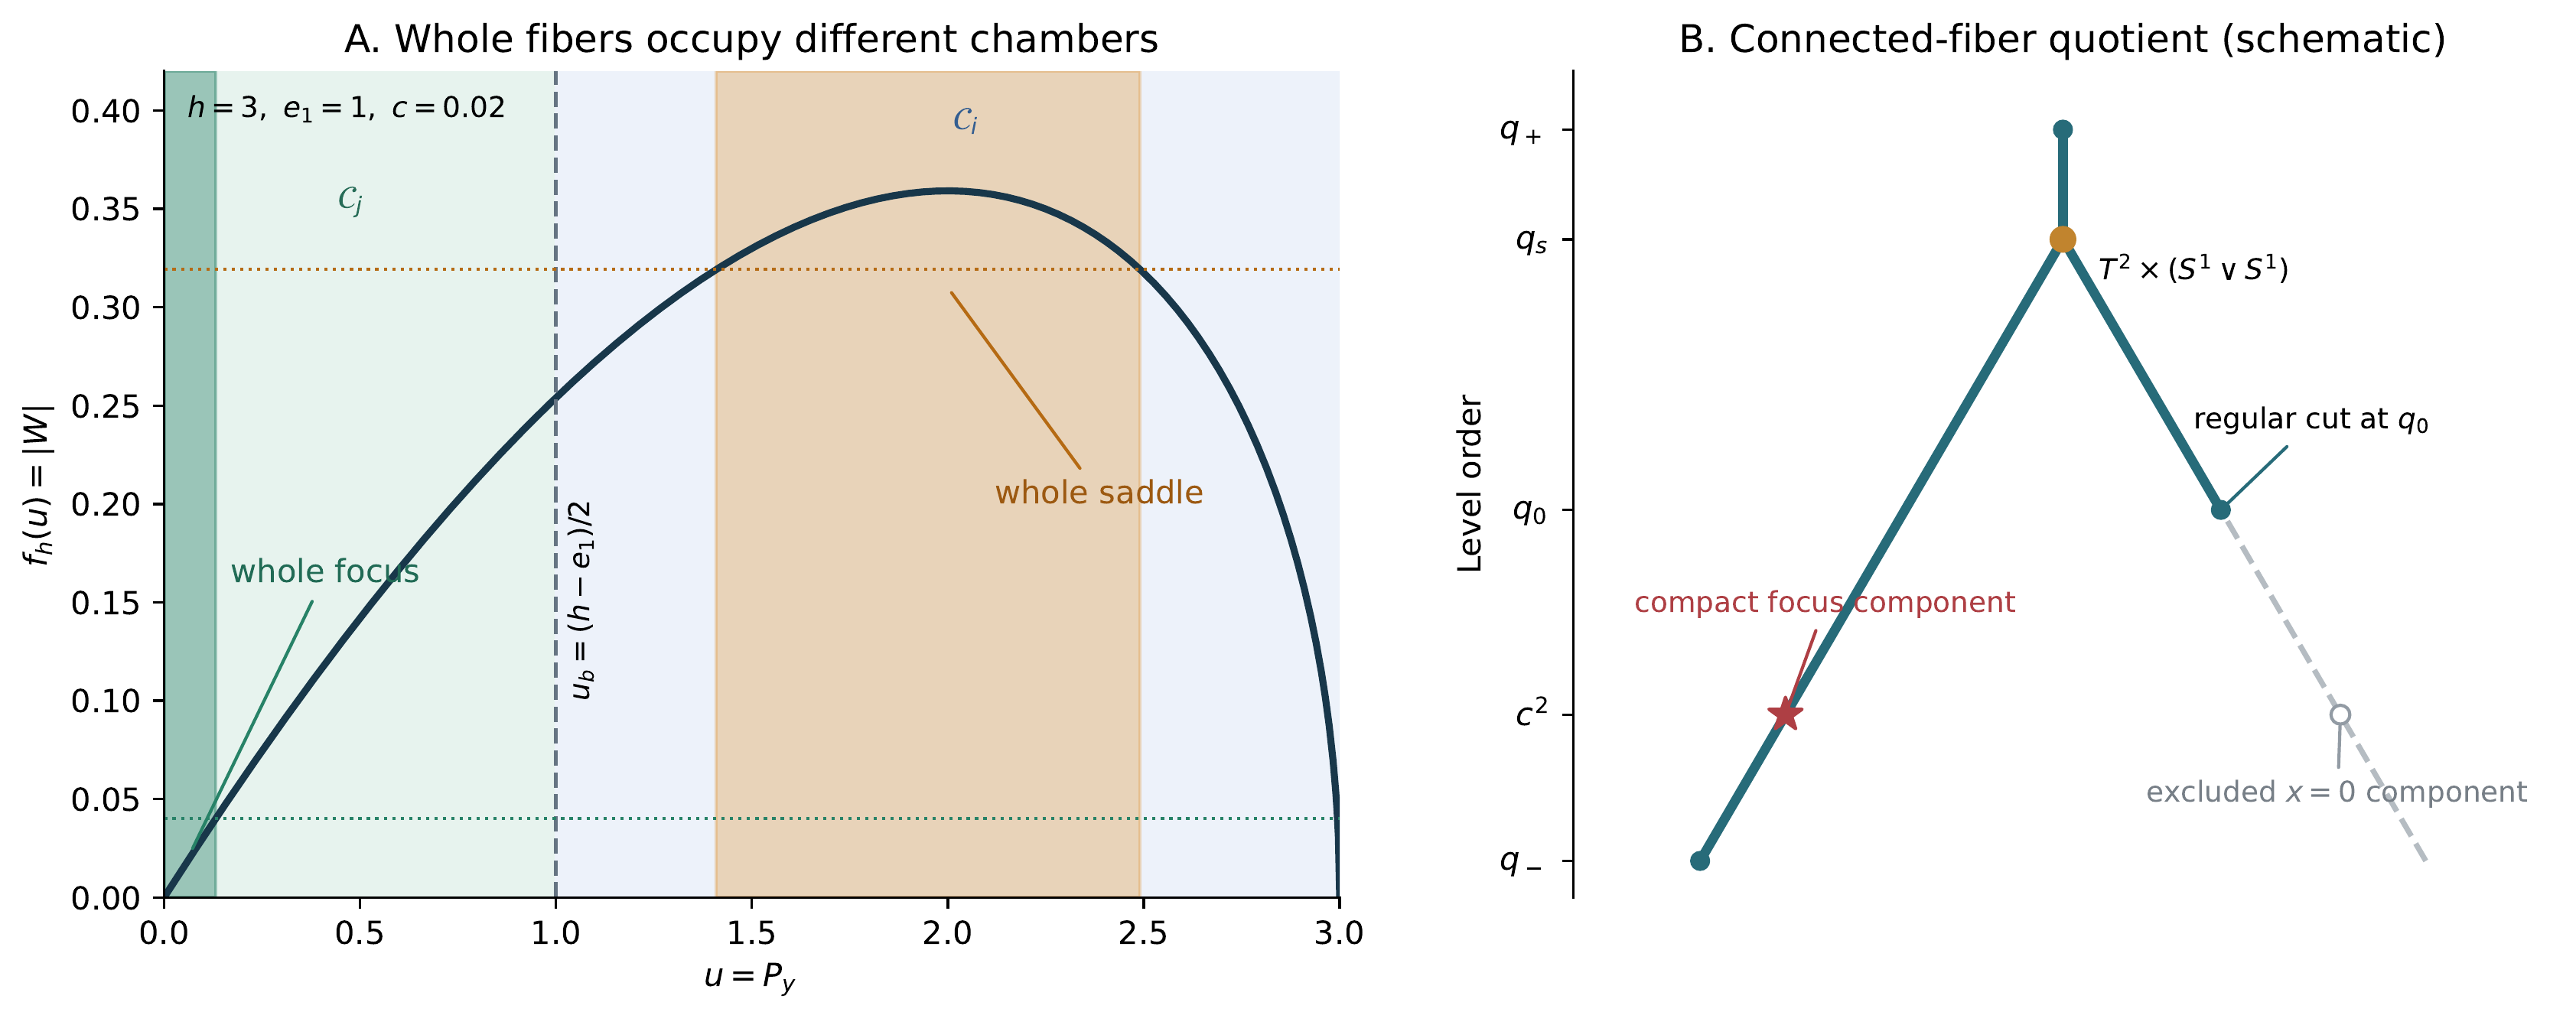
\includegraphics[width=\textwidth]{positive_transport_geometry.png}
\caption{左は chosen graph form における whole focus と whole saddle の chamber 分離。
右は annular insertion に用いる connected-fiber quotient の模式的な断面で、縦方向は level の順序だけを表す。
Upper leg の $q_0>c^2$ での切断により $x=0$ を含む成分を除き、lower focus と true saddle を保持する。
図の $q_0$ は本文の $q_*$ に対応する。}
\label{ai:figure}
\end{figure}

\subsection{明示的な annular embedding と primitive の定数項}

標準 normal tube を
\[
 \mathcal T=(I_-,I_+)\times S^1_\theta\times\CC^2_{Y,Z},\qquad
 \lambda_{\mathcal T}=I\,d\theta+\rho_Yd\theta_Y+\rho_Zd\theta_Z,
 \qquad\Omega_{\mathcal T}=d\lambda_{\mathcal T}
\]
とする。$b\in(I_-,I_+)$、$k\in\ZZ$ を任意に固定する。
$s>0$ に対し、$\{x\ne0\}$ の上で
\begin{equation}\label{ai:embedding}
 \theta=\frac{\arg x}{2\pi},\qquad
 Y=\sqrt{s}\,e^{2\pi i(k-1)\theta}y,\qquad Z=\sqrt{s}\,z,
 \qquad I=b+s\bigl(\rho_x-(k-1)\rho_y\bigr)
\end{equation}
と定める。

\begin{theorem}\label{ai:insertion}
任意の $k\in\ZZ$ と任意に小さい normal radius に対し、
$s>0$ を十分小さく取れば式\eqref{ai:embedding}は $K$ の開近傍を
$\mathcal T$ のその radius 内へ埋め込む。
この写像 $\iota_s$ は
\begin{equation}\label{ai:primitive}
 \iota_s^*\lambda_{\mathcal T}=s\lambda_0+b\,d\theta,
 \qquad \iota_s^*\Omega_{\mathcal T}=s\omega_0
\end{equation}
を満たす。従って $K$ の compact Lagrangian fibers、focus fibers、saddle fibers は
全て同時に actual な Lagrangian fibers へ移る。

像上の commuting integrals は
\begin{align}
 H&=I-b+k\rho_Y,& J&=\rho_Y-\rho_Z,\label{ai:integrals}\\
 W&=\sqrt{\frac{I-b+(k-1)\rho_Y}{\pi}}\,
       e^{-2\pi ik\theta}YZ,& Q&=|W-s^{3/2}c|^2.\label{ai:W}
\end{align}
Pullbacks はそれぞれ $sH_0,sJ_0,s^{3/2}W_0,s^3Q_0$ である。
Square root の中身は像の近傍で正である。
Focus axis における mixed coefficient の clockwise winding は、tube の frame に関して $k$ である。
\end{theorem}

\begin{proof}
式\eqref{ai:embedding}より
\[
 \iota_s^*(\rho_Yd\theta_Y)
 =s\rho_y\bigl(d\theta_y+(k-1)d\theta\bigr),
 \qquad \iota_s^*(\rho_Zd\theta_Z)=s\rho_zd\theta_z.
\]
$I\,d\theta$ と加えると、$\rho_y d\theta$ の補正が厳密に消え、
式\eqref{ai:primitive}を得る。Inverse は
\[
 x=\sqrt{\frac{I-b+(k-1)\rho_Y}{\pi s}}e^{2\pi i\theta},\quad
 y=s^{-1/2}e^{-2\pi i(k-1)\theta}Y,\quad z=s^{-1/2}Z
\]
である。$K$ 上では $\rho_x$ が正の下界を持つので、正の square root の領域に
少し大きい開近傍を取れ、そこで滑らかな embedding になる。
$K$ 上の $\rho_x,\rho_y,\rho_z$ は有界であるから、$I-b=O(s)$、
$|Y|,|Z|=O(\sqrt s)$ が一様に成り立つ。
これにより任意に小さい tube へ、全 compact fibers を保って入れられる。

式\eqref{ai:integrals}--\eqref{ai:W}の pullback は直接代入で分かる。
定数倍の symplectic form に対しても Poisson commutativity と Lagrangian 性は保たれる。
Zero section 上の focus locus では $I-b>0$ であり、
$Q$ の mixed quadratic coefficient は、正の実数倍と一定の非零実数を除けば
$e^{-2\pi ik\theta}$ である。Clockwise boundary での winding は $k$ となる。
\end{proof}

\begin{remark}[保持する marked periods]
任意の closed cycle $\gamma\subset K$ に対して、厳密に
\begin{equation}\label{ai:period}
 \int_{\iota_s\gamma}\lambda_{\mathcal T}
 =s\int_\gamma\lambda_0+b\,\deg(\theta|_\gamma)
\end{equation}
である。$b\,d\theta$ を exact term として捨ててはいけない。
Transverse cycle の $\theta$-degree が零なら、その action は $s$ 倍される。
Longitudinal circle の action には $b$ が加わる。
Hamiltonian $H$ の flow は周期 $1$ だが、primitive との contraction は
$\lambda_{\mathcal T}(X_H)=H+b$ である。
ここでは $\iota_{X_H}\Omega=-dH$ の規約を用いている。
\end{remark}

\begin{remark}[Disk-extension と semistable phase]
本定理の winding $k$ は、選んだ tube frame に関する値である。
Tube frame を actual semistable determinant frame の Hermitian 規格化から選べば、
これがそのまま central-frame winding になる。
第\ref{pw:semistable-phase}項の original-coordinate comparison における $+1$ を
さらに加えることはしない。本定理では式\eqref{ai:embedding}により新しい normal first jet を選んでいる。
特に original-coordinate identity $y=tY/x$ を保つ symplectic comparison を構成したわけではない。
Frame と action は有限 annulus 上では滑らかだが、同じ選択が deleted disk へ延びるとは限らない。
この点が第\ref{cw:section}節の disk-extending rigidity との両立理由である。
\end{remark}

\subsection{所定の K\"ahler form に対する actual tube}

\begin{lemma}[First jet を指定した annular neighborhood]
\label{ai:actual-tube}
$(X,\omega)$ を symplectic 六次元多様体、$C\subset X$ を symplectic surface、
$A\subset C$ を compact annulus とする。
$\omega|_A=dI\wedge d\theta$ と area coordinates を取り、
symplectic normal bundle の unitary frame を $A$ 上で選ぶ。
このとき、十分小さい標準 tube $\mathcal T$ から $X$ への symplectic embedding $\Psi$ があり、
zero section は $A$ へ恒等的に写り、normal first jet は指定した frame と一致する。
既に一つの小さい collar 上でこのような embedding が指定されていれば、
その collar を縮めた上で embedding 全体を厳密に保つ relative 版も成立する。
\end{lemma}

\begin{proof}
Symplectic normal を $TC^\omega$ とし、指定 frame と base の恒等写像から
zero section 上の symplectic linear isomorphism を作る。
これを smooth tubular embedding $F$ に延長する。
$F^*\omega$ と $\Omega_{\mathcal T}$ は zero section 上で full bilinear forms として一致する。
差を $\Delta$ と書く。Normal radial homotopy によって
$\Delta=d\alpha$、$\alpha=O(|v|^2)$ を得る。
十分小さい tube では直線経路 $\Omega_{\mathcal T}+u\Delta$ が symplectic であり、
$\iota_{V_u}(\Omega_{\mathcal T}+u\Delta)=-\alpha$ の Moser field は $V_u=O(|v|^2)$ となる。
従ってその flow は zero section と first jet を固定する。
Compactness により共通の小さい tube 上で time $1$ まで定義され、所要の $\Psi$ を得る。
Prescribed collar で $F$ を既存の embedding と一致させれば $\Delta=0$、
radial primitive も零となるため、Moser flow はそこで恒等である。
これは symplectic neighborhood theorem の relative Moser 証明である
\cite[\S7.3, Theorem 7.4]{cds-local}。
\end{proof}

K\"ahler 多様体内の complex curve collar を扱う場合にも、
complex normal frame が所定の K\"ahler metric に関して直交するとは限らない。
ただし一つの complex normal line を選び、それと Hermitian complement を使うことはできる。
Gram--Schmidt の diagonal coefficients を正に取ると、complex determinant は正実数倍なので、
元の determinant frame に対する winding は変わらない。
この操作は一方の line を保持するが、指定された二つの非直交な normal lines の両方を保持しない。
その両方を固定することは、本節の結論に含めない。

\begin{corollary}[Actual K\"ahler annulus 内の branched block]
\label{ai:actual-insertion}
補題\ref{ai:actual-tube}の任意の actual tube に対し、任意の整数 $k$ の winding を持つ
compact block $\Psi(\iota_s(K))$ が、十分小さい $s>0$ について存在する。
その全 fibers と singularity types は命題\ref{ai:compact-block}の通りであり、
元の $\omega$ に関して Lagrangian である。
Actual form が coordinate torus rotations に不変であることは必要ない。
Hamiltonian actions も $\Psi\circ\iota_s$ により同時に移送する。
\end{corollary}

Actual tube 上に primitive $\lambda_X$ が既に指定されている場合にも、
その $A$ 上の circle period を用いて $I$ の additive constant を決めれば、
$\Psi^*\lambda_X-\lambda_{\mathcal T}$ の $H^1(\mathcal T;\RR)$ class は零となる。
従ってこの差は exact であり、式\eqref{ai:period}は同じ marked cycles に対してそのまま成り立つ。
Additive constant と配置する $b$ は、primitive の period データとして保持する。
所定の global primitive がなくても、$H^2(\mathcal T;\RR)=0$ により local primitive は選べる。

\subsection{一つの curve end との whole-fiber 一致}

式\eqref{ai:embedding}の像上で
\[
 \widehat H=H+b=I+k\rho_Y,\qquad
 U=e^{-2\pi ik\theta}Y,\qquad V=Z
\]
と置くと、厳密に
\begin{equation}\label{ai:end-coordinates}
 \lambda_{\mathcal T}=\widehat H\,d\theta+\rho_Ud\theta_U+\rho_Vd\theta_V,
 \quad J=\rho_U-\rho_V,
 \quad W=\sqrt{\frac{\widehat H-b-\rho_U}{\pi}}\,UV
\end{equation}
となる。すなわち、一次共役因子の decreasing radial family が
$a=\widehat H-b$ としてそのまま現れる。
この式は単なる quadratic approximation ではなく、compact lower component 全体での恒等式である。

\begin{theorem}[一つの actual positive-winding end の接着]
\label{ai:one-end}
$\bar C\subset(X,\omega)$ を compact symplectic surface with boundary とし、
boundary components の数を $n\ge2$ とする。
一つの boundary collar に補題\ref{ai:actual-tube}の tube を選ぶ。
他の端の fibration と normal frames を自由に選んでよいとする。
このとき、任意の $k\in\ZZ$ に対し、十分小さい annular branched block と
curve block を actual $\omega$ の上で接ぐことができる。
接着部分は lower compact focus component の saturated collar であり、
両側の actual fibers、period-one circle actions、marked primitive periods は厳密に一致する。
Corner の内部には whole $T^2\times(S^1\vee S^1)$ saddle fiber が残る。
他の artificial boundary faces の消失は主張しない。
\end{theorem}

\begin{proof}
第\ref{pw:m1}項の $F_1>2c$ の範囲で、$j=0,q=c^2$ の lower component を含む
小さい compact $(j,q)$-window を取る。Lower root と upper root の間には一様な gap がある。
従って window を縮めれば、選んだ $H$-interval 上で全 lower fibers を一つの normal tube に入れられる。
具体的な cutoff 不等式は補題\ref{pe:uniform}による。
式\eqref{ai:end-coordinates}をそのまま curve block の prescribed collar germ とする。

Normal first jet は、tube frame に対して $U$-direction を $e^{2\pi ik\theta}$ 倍する。
この first jet は annulus 上では unitary である。Disk への延長は要求しない。
$n\ge2$ の surface では、一つの boundary circle に指定した $S^1$-valued frame の degree を
別の自由な boundary で相殺できる。従って二つの individual frames と tensor frame は
$\bar C$ 上へ延長できる。
これは $H^2(\bar C;\ZZ)=0$ と、一つの boundary への
$H^1(\bar C;\ZZ)\to H^1(S^1;\ZZ)$ の全射性からも従う。

この延長を用いて dual connections を選び、指定 collar 上では connection forms を厳密に零とする。
Curve の Morse function と正の radial parameter $a$ は、指定 collar で
$a=\widehat H-b$ となるように選び、critical levels の近くでは必要な一定値にする。
定理\ref{pe:two-end}の一端だけを指定する構成により compact curve fibers を得る。
Normal radii は共通に十分小さく取る。

Curve model の embedding は、指定 collar 上では既に得た actual embedding と一致させる。
その first jet は上で global normal bundle へ延長されている。
Tubular embedding をこの germ に合わせて延ばし、補題\ref{ai:actual-tube}の relative Moser を使うと、
collar 全体を固定して actual $\omega$ へ移せる。
したがって germ だけでなく、その domain に含まれる compact focus fiber 全体と近傍 fibers が一致する。

Primitive は collar 上で式\eqref{ai:end-coordinates}を使用する。
Base primitive のこの一つの boundary period は、他の自由な boundary periods を調整して延長できる。
よって longitudinal shift $b$ を含む marked periods が一致する。
ここで relative embedding を固定する collar は、lower fibers だけでなく
$\iota_s(K)$ 全体を式\eqref{ai:end-coordinates}で表示できる normal neighborhood を含むものとする。
必要なら zero-section collar を少し延長してから切断位置を選ぶ。
$K$ はこの共通座標で $\widehat H\in b+s\,\operatorname{pr}_h R$ に射影し、
normal radii は一様に $O(\sqrt s)$ なので、十分小さい $s$ に対してこの選択ができる。
共通 collar 上では、curve block の $(J,Q)$-window と lower-root cutoff によって
交わりを lower connected components に限定する。
Collar 外も同じ global normal embedding を用いるので、その単射性により余分な交わりは生じない。
指定 collar の両側を切って接げば、共通の actual fibers を持つ一つの compact assembly となる。
\end{proof}

\subsection{半安定超曲面における適用範囲}

\begin{proposition}[二つの normal lines への winding の配分]
\label{ai:distributed}
整数 $a,d$ に対し、式\eqref{ai:embedding}を
\begin{equation}\label{ai:distributed-map}
\begin{aligned}
 Y&=\sqrt{s}\,e^{2\pi i(a-1)\theta}y,&
 Z&=\sqrt{s}\,e^{2\pi id\theta}z,\\
 I&=b+s\bigl(\rho_x-(a-1)\rho_y-d\rho_z\bigr)
\end{aligned}
\end{equation}
で置き換えても、式\eqref{ai:primitive}と全 compact fibers の挿入が成り立つ。
その winding は $k=a+d$ であり、像上では
\begin{align}
 H&=I-b+a\rho_Y+d\rho_Z,& J&=\rho_Y-\rho_Z,\label{ai:distributed-H}\\
 W&=\sqrt{\frac{I-b+(a-1)\rho_Y+d\rho_Z}{\pi}}
          e^{-2\pi i(a+d)\theta}YZ.\label{ai:distributed-W}
\end{align}
端の product coordinates は
\begin{equation}\label{ai:distributed-end}
 \widehat I=I+a\rho_Y+d\rho_Z,\quad
 U=e^{-2\pi ia\theta}Y,\quad V=e^{-2\pi id\theta}Z
\end{equation}
であり、
\[
 \lambda_{\mathcal T}=\widehat I\,d\theta+\rho_Ud\theta_U+\rho_Vd\theta_V,
 \qquad W=\sqrt{\frac{\widehat I-b-\rho_U}{\pi}}\,UV.
\]
従って、二つの normal first jets の twists を $a,d$ として個別に指定できる。
\end{proposition}

\begin{proof}
$\rho_Yd\theta_Y$ と $\rho_Zd\theta_Z$ が作る angular terms はそれぞれ
$s(a-1)\rho_y d\theta$ と $sd\rho_zd\theta$ であり、$I\,d\theta$ の補正と消える。
Square root の中身は再び $s\rho_x/\pi$ である。
式\eqref{ai:distributed-H}の pullback は $sH_0$、
式\eqref{ai:distributed-W}の pullback は $s^{3/2}W_0$ となる。
最後の strict identity は式\eqref{ai:distributed-end}を代入すれば従う。
\end{proof}

$C_{56}$ の deleted disks の外では半安定射は submersion であり、
compact curve block の近傍を十分小さい $t=\tau\ne0$ へ移せる。
一つの collar では $(x,T,Y,z)=(x,\tau/x,0,0)$ という明示的な curve family がある。
Local lift をこの family に沿わせ、collar 外へ partition of unity で延ばすことにより、
central $\bar C_{56}$ の lift を、この actual collar と一致するように選べる。
Chosen family の fiberwise K\"ahler form に関して symplectic 性は compactness と openness により保たれる。
この actual symplectic surface の collar に系\ref{ai:actual-insertion}と定理\ref{ai:one-end}を適用する。
その frame を central semistable determinant frame から選べば、$k=1$ または $k=2$ を直接実現できる。

これは $\tau\ne0$ を固定した有限長の neck における actual one-end statement である。
$\tau\to0$ で共通の normal radius を持つこと、whole exceptional sphere に延びること、
所定の全 normal circles と全 corner faces を保存することは主張しない。
特に、$k$ を変える frame は deleted disk へ延びるとは限らない。
また、ここで挿入した block は actual curve collar 内の局所的な置換であり、
残る geometric corner 全体の充填ではない。

任意に指定された smooth hypersurface と K\"ahler form へは、
第\ref{lc:application-local}項の deformation と Moser の議論を assembly 全体へ適用できる。
この最後の移送は actual fibers の一致を保つが、元の代数的 strata の位置まで固定するものではない。

\subsection{$C_{56}$ の全24 annular ends に対する同時構成}

一つの端では tensor winding だけを指定すればよいが、全ての端を同時に扱う際には
二つの individual line bundles の degree も合わせる必要がある。
$C_{56}$ では、orthogonalized normal splitting を
\[
 E_+\simeq\mathcal O_C(1),\qquad E_-\simeq\mathcal O_C(5)
\]
と選ぶ。第一の line を保持し、第二の holomorphic quotient を Hermitian complement へ移す。
この smooth complex identification の determinant は正実数に規格化できるので、
determinant frame の phase を余分に変えない。
ここで tube の $Y,Z$ はこの $E_+,E_-$ の coordinates であり、
以前の algebraic coordinates の名前と自動的に同一視しない。

$\bar C=C_{56}\setminus\bigcup_{i=1}^{24}D_i$ 上で
\begin{equation}\label{ai:individual-sections}
 \sigma_+=L_1|_C,\qquad
 \sigma_-=L_1L_2^2L_3L_4|_C
\end{equation}
は非消失である。Hermitian norm で規格化して global unitary frames $u_+,u_-$ を得る。
その tensor は、位相の意味で
$\sigma=L_1^2L_2^2L_3L_4$ と一致する。
各 deleted disk の local unit を frame に吸収すると、collar 上で
\[
 u_+=e^{2\pi ia_i\theta_i}f_{i,+},\qquad
 u_-=e^{2\pi id_i\theta_i}f_{i,-}
\]
と書ける。$f_{i,\pm}$ はそれぞれの disk frame に winding 零で対応する unitary frames である。
Twists は次の表になる。
\begin{center}
\begin{tabular}{c|c|c|c|c}
端の型&個数&$a_i$&$d_i$&$k_i=a_i+d_i$\\\hline
$L_1=0$&6&1&1&2\\
$L_2=0$&6&0&2&2\\
$L_3=0$&6&0&1&1\\
$L_4=0$&6&0&1&1
\end{tabular}
\end{center}
従って individual sums は $\sum_i a_i=6$, $\sum_i d_i=30$ であり、
determinant sum は $\sum_i k_i=36$ である。

\begin{theorem}[全24端の annular assembly]
\label{ai:c56-allends}
第\ref{lc:application-local}項の actual $\bar C_{56}$ の近傍において、
十分小さい固定した $t=\tau\ne0$ を取る。
Normal actions と frames を構成の一部として選んでよいとする。
このとき、次を同時に満たす compact な Lagrangian-fiber assembly を、
その actual K\"ahler form の上で構成できる。
\begin{enumerate}
\item Curve block は genus $10$、$24$ boundary components の surface に基づき、
      $42$ 個の index-$1$ Morse critical points と compact focus normal fibers を持つ。
      従来の $42$ 個の $(\text{once-pinched }T^2)\times(S^1\vee S^1)$ fibers は保持される。
\item 全24端に、命題\ref{ai:compact-block}の compact branched block を互いに素に挿入する。
      各端の lower compact focus collar は curve block と actual fibers で一致する。
\item Semistable determinant frame に関する winding は上の表の $2,2,1,1$ であり、
      individual normal line の degrees $6,30$ も同時に一致する。
\item 一つの global base primitive に由来する boundary periods を用い、
      全ての overlaps で marked periods と周期格子を保つ。
\end{enumerate}
各挿入 block には whole smooth-saddle fiber $T^2\times(S^1\vee S^1)$ がある。
追加した annular focus fibers と saddle fibers はともに Euler 数 $0$ である。
この構成は残る branch legs と outer faces を自由境界として残し、
幾何学的 corner cores、全 exceptional spheres、他の component regions の充填は主張しない。
\end{theorem}

\begin{proof}
まず central $\bar C$ と、その deleted disk の中心を避けた少し大きい compact collars を、
半安定射の regular locus 内で固定する。
Actual smooth fiber への移送は、選んだ collars 上の normal frame data とともに行う。
K\"ahler normal metric による第一の line と orthogonal complement の選択は、
これらの relative complex bundle classes を変えない。
式\eqref{ai:individual-sections}の frames は actual curve 上へ運ばれ、
全24端の個別の first jets は既に一つの global normal bundle の frames に延びている。

\emph{Primitive の選択。}
$H^2(\bar C;\RR)=0$ なので $d\beta=\omega_C$ となる一つの $\beta$ を選ぶ。
Actual neighborhood に primitive が指定されていれば、その restriction を用いる。
各 collar で $\omega_C=dI_i\wedge d\theta_i$ と書く。
$\beta-I_i d\theta_i$ の period を $I_i$ の additive constant で補正すると、差は exact になる。
その primitive を disjoint collars の cutoff により global に補正すれば、
全 collars で同時に
\begin{equation}\label{ai:global-primitive}
 \beta=I_i d\theta_i
\end{equation}
とできる。この操作は $\beta$ の cohomological periods を変更しない。
各 $I_i$ の additive constant はこの一つの $\beta$ により決まり、独立には指定しない。
特に $\theta_i$ を deleted disk に関して反時計回りに取り、boundary を $I_i$ の level とすれば
\begin{equation}\label{ai:stokes}
 \int_{\bar C}\omega_C=-\sum_{i=1}^{24}I_i(\partial_i\bar C).
\end{equation}
全ての $I_i$ を正にする条件は課さない。

\emph{全 collars の actual embedding。}
Global unitary frames $u_\pm$ に関して dual connections を選び、
その connection forms を全 collars で零にする。両方を global frames に関して flat に選んでもよい。
各 collar の unrotated frames $f_{i,\pm}$ で補題\ref{ai:actual-tube}の actual tube を作る。
式\eqref{ai:distributed-end}の shear を合成すると、
global normal model の coordinates $(\widehat I_i,\theta_i,U,V)$ から actual tube への
strict symplectic embedding となり、その normal first jet はちょうど $u_\pm$ である。
これらの prescribed germs は互いに素な collars にあり、first jets は既に global に延びている。
従って relative tubular embedding と radial Moser の証明により、
全ての germs を同時に厳密に保つ一つの global normal-neighborhood embedding が得られる。
ここで actual primitive の pullback は、式\eqref{ai:global-primitive}の選択により、
model primitive と exact term だけ異なる。従って marked periods は一致する。

\emph{共通の縮小と radial parameter。}
命題\ref{ai:compact-block}の一つの source block $K$ を全24端で使う。
$R$ の $h$-interval の中心を $h_0>0$ とする。
各 actual collar 内に center level $I_i^0$ を選び、
\begin{equation}\label{ai:offsets}
 b_i=I_i^0-sh_0
\end{equation}
と置く。命題\ref{ai:distributed}を $(a_i,d_i,b_i)$ で用いると、
normal-model base coordinate は
$\widehat I_i=b_i+sH_0$ であり、その image は $I_i^0$ を中心とする幅 $O(s)$ の collar に入る。
全 normal moments は $O(s)$、通常の normal radius は $O(\sqrt{s})$ である。
有限個の disjoint tubes と共通の global normal embedding に対し、
十分小さい一つの $s>0$ を選べば全24個の $K$ が同時に入る。

Curve 上の Morse function $h$ は、incoming と outgoing の両方を持つ index-$1$ cobordism として選ぶ。
各 collar では $h=\chi_i(\widehat I_i)$ とし、
incoming では $\chi_i'>0$、outgoing では $\chi_i'<0$ とできる。
例えば incoming を一つ、outgoing を23個とし、$42=2\cdot10+24-2$ 個の saddles を取る。
全端で $h=+\widehat I_i$ と要求してはいけない。
Longitudinal action $\widehat I_i$ と base label $h$ はこの monotone relabeling により区別する。

Positive radial parameter $\mathfrak a_s$ を Reeb graph 上の関数として選び、
指定 collar では
\[
 \mathfrak a_s=\widehat I_i-b_i,
 \qquad c_s=s^{3/2}c_0
\]
とする。ここで $c_0$ は source block の $c$ である。
全 critical points の近くでは $\mathfrak a_s$ を一定にし、
$sA_0\le\mathfrak a_s\le sB_0$ となる共通の $A_0,B_0>0$ を取れる。
Reeb edges ごとの prescribed collar functions は有限個なので、この正の延長に障害はない。
Normal integral を
\[
 J=\rho_U-\rho_V,\qquad
 Q_s=\left|\sqrt{\frac{\mathfrak a_s-\rho_U}{\pi}}\,UV-c_s\right|^2
\]
とする。全 collars で、式\eqref{ai:distributed-end}の full nonlinear integral と一致する。

小ささ条件は scale を含めて確認できる。
$0<\delta<1/2$、小さい $\vartheta>0$、$j_*>0$ を
\[
 j_*<\delta A_0/2,\qquad
 \pi^3(1+\sqrt{1+\vartheta})^2c_0^2
 <\frac{\delta^2(1-\delta)}2A_0^3
\]
となるように選ぶ。$c_0$ と $R$ は最初にこれらを満たすように取る。
Window を
\[
 |J|\le s j_*,\qquad |Q_s-c_s^2|\le\vartheta c_s^2
\]
とすると、$\rho_U=s\tilde u$, $J=s\tilde j$, $\mathfrak a_s=s\tilde a$ の代入により、
補題\ref{pe:uniform}の radial inequalities は全て $s^3$ を共通因子として持つ。
従って lower fibers は一様に cutoff $\rho_U=\delta sA_0$ を避ける。
Source window を $q_-< (1-\vartheta)c_0^2<(1+\vartheta)c_0^2<q_*$ の中に選び、
$j_*$ を $R$ の $j$-width より小さくすれば、この window は各 $K$ の lower leg に入る。
全 curve fibers は compact であり、normal radius は $O(\sqrt{s})$ なので
上の actual normal embedding の domain に入る。

定理\ref{pe:two-end}と同じ Poisson-commutativity と relative-extension の証明を、
今回既に global に整合した全 collar data に適用する。
Shared collar の全 fibers は同じ式を持つので、全24箇所で厳密に接ぐことができる。
Global normal embedding の単射性と collars の disjointness により、別の挿入同士の余分な交わりはない。
Saddle の近くで $\mathfrak a_s$ は一定なので、curve 側の同時 node--saddle 型も保持される。
各 annular block の whole saddle fibers は window の外側にも残り、
それらを含む全 $K$ を最初から同じ actual embedding で移している。
最後に $b_i$ を含む式\eqref{ai:period}と式\eqref{ai:global-primitive}により、
全 overlaps の marked periods と周期格子が一致する。
\end{proof}

\begin{corollary}[この有限 assembly の商]
\label{ai:assembly-quotient}
定理\ref{ai:c56-allends}の finite compact assembly には共通の smooth integrals
$G=(J,Q_s,h)$ があり、各 annular piece では
$h=\chi_i(b_i+H)$ とする。
その connected-fiber quotient は compact Hausdorff であり、
regular fibers は connected $T^3$ である。
これはこの assembly に対する主張であって、$X_6$ 全体に対する主張ではない。
\end{corollary}

\begin{proof}
Integrals は共通の collar 上で文字通り一致するので貼り合う。
各切断は connected fibers の全体を保つものを使う。
共通 collar の端で必要となる角の整形は、正則な base faces の関数を用いて行い、
whole fibers と記載した特異 strata を保つ。
Compact metric domain の points $p_n,q_n$ が同一の connected fiber component $C_n$ にあり、
$p_n\to p$, $q_n\to q$ とする。
Compact subsets の Hausdorff topology で subsequence を取ると、
$C_n$ は nonempty compact connected set $C$ に収束する。
$C$ は $p,q$ を含み、$G$ の continuity により一つの limiting fiber に含まれる。
従って $p,q$ も同じ connected component に属する。
よって fiber-component equivalence relation は閉であり、compact Hausdorff domain の商は Hausdorff である。
Regular components は whole compact tori のまま接がれているので $T^3$ である。
\end{proof}

\begin{remark}\label{ai:all24-scope}
この同時構成で解決したのは、一つの $C_{56}$ block の全24 annular ends における
位相・個別 normal frames・primitive periods・compact fibers の相対整合である。
各端の residual branch legs と outer cuts は残る。
異なる curve blocks に接する一つの geometric corner core を同時に埋めたわけではなく、
free boundary のない $X_6$ 全体の fibration は依然として未構成である。
全24端に採用した actions は transported actions であり、
所定の divisor-normal circles と disk-extending first jets を全て保持する条件は課していない。
また $\tau\to0$ と $s\to0$ の同時一様比較は主張しない。
\end{remark}

\section{正 winding 模型の regular wall の保周期的な整形}
\label{we:section}

第\ref{tp:section}節の chosen graph form に対する比較を、central component wall の近傍へ延長する。
新しい foliation は fixed nonzero slice で旧 foliation と Hamiltonian 同値であり、
指定した whole focus end と whole saddle fiber の近傍では同一である。
従って新しい critical points を作らず、全 marked actions も保つ。
Central slice の通常の elliptic collapse と、nonzero slice に新たな singularity を作ることを区別する。

\subsection{Regular lower annulus の action}

標準一次共役因子模型で
\[
 H=P_x+P_y,\quad J=P_y-P_z,\quad u=P_y,\quad
 W=\bar X_1X_2X_3,\quad Q=|W-c|^2
\]
とする。Dense torus の周期 $1$ の角を
\[
 \alpha=\theta_1,\quad \beta=-\theta_3,\quad
 \phi=-\theta_1+\theta_2+\theta_3
\]
と変換すれば integral unimodular であり、
\begin{equation}\label{we:primitive}
 \lambda_{\rm std}=H\,d\alpha+J\,d\beta+u\,d\phi,\qquad
 \omega_{\rm red}=du\wedge d\phi
\end{equation}
となる。固定した $(h,j)$ に対し
\[
 L=\max(0,j),\quad
 f(u)=\frac{\sqrt{(h-u)u(u-j)}}{\pi^{3/2}},
 \quad L<u<u_1,\quad F=f(u_1)
\]
を lower radial branch と書く。
$F>2c$ とし、$c^2<q<(F-c)^2$ とする。
Lower reduced circle は global graph
\begin{equation}\label{we:graph}
 u=U(h,j,q,\phi)
 =f_{h,j,-}^{-1}\left(c\cos(2\pi\phi)
       +\sqrt{q-c^2\sin^2(2\pi\phi)}\right)
\end{equation}
であり、$U_q>0$ である。
従って
\begin{equation}\label{we:action}
 I(h,j,q)=\int_0^1U(h,j,q,\phi)\,d\phi
\end{equation}
は smooth で $I_q>0$ を満たす。

\begin{lemma}[壁を含む regular annulus]\label{we:annulus}
Compact parameter rectangle $R$ 上で smooth functions $b_-<b_+$ が
\[
 L<b_-<b_+<u_1,\qquad f(b_-)>2c,\qquad F-f(b_+)>2c
\]
を一様に満たすとする。
このとき $c^2<q_a<q_b<(F-c)^2$ を smooth に選んで
\[
 U(h,j,q_a,\phi)<b_-<b_+<U(h,j,q_b,\phi)
\]
を全 $\phi$ について成立させられる。
従って $[b_-,b_+]$ 内の全 constant circles は、
whole focus end と whole saddle fiber の間の同じ regular annulus に入る。
\end{lemma}
\begin{proof}
例えば
\[
 q_a=\frac{c^2+(f(b_-)-c)^2}{2},\qquad
 q_b=\frac{(f(b_+)+c)^2+(F-c)^2}{2}
\]
と置く。$u=b_-$ 上の $Q$ の最小値は $(f(b_-)-c)^2$、
$u=b_+$ 上の最大値は $(f(b_+)+c)^2$ であり、lower branch の単調性を使えばよい。
\end{proof}

\subsection{Hamiltonian straightening}

\begin{theorem}[全作用を保つ相対整形]\label{we:straightening}
補題\ref{we:annulus}の条件の下で、$H,J$ と可換な compactly supported
Hamiltonian isotopy $\psi_t$ があり、次を満たす。
保護する focus end の window は $q<q_a$、saddle neighborhood は $q>q_b$ に取る。
Strict gaps により、それぞれ whole singular fiber を含むこのような近傍を選べる。
あらかじめ指定した end window を点ごとに保つ場合には、
その window と support annulus の非交差を追加の相対条件とする。
\begin{enumerate}
\item Support は上記 regular lower annulus に入り、whole focus end と
  whole saddle fiber の共通近傍では $\psi_t=\mathrm{id}$ である。
\item $Q^\natural=Q\circ\psi_1^{-1}$ と置けば、$b_-<u<b_+$ の full neighborhood で
  \begin{equation}\label{we:toric}
   Q^\natural=\mathcal Q(H,J,u),\qquad I(H,J,\mathcal Q(H,J,u))=u.
  \end{equation}
  従ってその葉は full toric moment fibers である。
\item $H,J$、connected-fiber quotient、全 singularity types、
  transported marked actions と period lattice を保つ。
  特に新しい saddles、minima、degenerate critical points は作らない。
\end{enumerate}
$R$ を少し大きい rectangle の内部に取れば、その外周に恒等な isotopy として構成できる。
この場合、toric straightening の結論を主張する parameter set は内側の $R$ である。
\end{theorem}

\begin{proof}
\[
 U_t=(1-t)U+tI
\]
と置けば $(U_t)_q=(1-t)U_q+tI_q>0$ であり、$\int_0^1U_t\,d\phi=I$ である。
従って moving annulus 上で $u=U_t(q,\phi)$ の smooth inverse
$q=q_t(h,j,u,\phi)$ が存在する。

$I(q_a)<b_-<b_+<I(q_b)$ である。
少し大きい action interval $B(h,j)$ を選び、$[b_-,b_+]\Subset B$ とし、
その中の全 constant circles が元の regular annulus に入るようにする。
具体的には、下端を $f_-^{-1}(c+\sqrt{q_a})$ と $b_-$ の間、
上端を $b_+$ と $f_-^{-1}(\sqrt{q_b}-c)$ の間に取れる。
$\eta(h,j,I)$ を $[b_-,b_+]$ の近傍で $1$、$B$ の外で $0$ となる smooth cutoff とする。
周期関数
\[
 k(h,j,q,\phi)=\int_0^\phi
 \bigl(U(h,j,q,s)-I(h,j,q)\bigr)\,ds
\]
を定義する。Integrand の一周期の積分は零なので $k$ は well-defined である。
Moving annulus 上で
\begin{equation}\label{we:hamiltonian}
 K_t(H,J,u,\phi)=
 \eta(H,J,I(H,J,q_t))\,k(H,J,q_t,\phi)
\end{equation}
とし、その外では零とする。
Cutoff は moving annulus の両端で零なので smooth に延びる。
Support において $U(q,\phi)$ と constant $I(q)$ はともに元の protected annulus 内にある。
よってその convex combination $U_t$ もそこに入り、
$K_t$ の support は固定された compact regular annulus に一様に含まれる。
必要なら $H,J$ の少し大きい rectangle で parameter cutoff を掛ける。

規約 $\iota_{X_K}\omega=-dK$ の下で、graph $u=U_t(q,\phi)$ 上の normal velocity は
\[
 X_K^u-(U_t)_\phi X_K^\phi
 =-\partial_\phi(K_t|_{\text{graph }q}).
\]
$\eta=1$ の inner family では、右辺は $I-U=\partial_tU_t$ である。
従って flow は graph $U_0(q,\phi)$ を $U_t(q,\phi)$ へ送り、
時刻 $1$ には $u=I(q)$ へ送る。
$H,J$ derivatives は $\alpha,\beta$ の動きを追加するだけであり、$H,J$ 自体は一定である。
これで式\eqref{we:toric}を得る。

Support は prescribed singular fibers とその近傍から離れている。
新しい系は旧系の Hamiltonian conjugate なので、critical set と critical values は変更されず、
connected fibers と quotient は $\psi_1$ で同定される。
最後に
\[
 \frac{d}{dt}\psi_t^*\lambda_{\rm std}
 =d\left(\psi_t^*(\lambda_{\rm std}(X_{K_t})-K_t)\right)
\]
だから $\psi_t^*\lambda_{\rm std}-\lambda_{\rm std}$ は exact である。
従って全 closed marked cycles の actions が厳密に保たれる。
\end{proof}

\begin{remark}
Regular annulus 内では foliation を変更するが、protected focus end と saddle neighborhood では
点ごとに恒等である。従って、既に接いだ curve block を変えず wall の内部だけを処理できる。
単なる位相的な isotopy ではなく、actual symplectic form に対する Hamiltonian isotopy を使っている。
また annular insertion の primitive $s\lambda_{\rm std}+b\,d\theta_1$ についても、
support は $X_1\ne0$ にあり、isotopy による closed form $d\theta_1$ の変化は exact である。
従って affine offset を含む marked periods も変えない。
\end{remark}

\begin{remark}[Radial replacement の作用補正]\label{we:action-correction}
保周期的な radial integral は一般に $f(u)^2+c^2$ とは異なる。
$h,j,u$ が compact regular band にあるとして $c\to0$ とすると、
$v=f_-^{-1}$ に対して
\[
 I(q)=v(\sqrt q)+\frac{c^2}{4}
 \left(v''(\sqrt q)-\frac{v'(\sqrt q)}{\sqrt q}\right)+O(c^4)
\]
であり、従って
\[
 \mathcal Q(h,j,u)
 =f(u)^2+\frac{c^2}{2}
 \left(1+\frac{f(u)f''(u)}{f'(u)^2}\right)+O(c^4).
\]
これは式\eqref{we:graph}を $c$ で展開して一周期平均を取り、
$I(q)=u$ を解けば得られる。Odd powers は $\phi\mapsto\phi+1/2$ の対称性で消える。
単に角依存項を cutoff して $f^2+c^2$ に置換する操作には、この作用補正は含まれない。
\end{remark}

\subsection{一つの component wall}

$M_1=P_x-P_y=H-2u$ とし、wall $M_1=e_1$ の位置を
$b_1(h,j)=(h-e_1)/2$ とする。
一壁版では $R\Subset\{j<e_2\}$ として、
この hyperplane が実際の $D_i$--$D_j$ wall になる領域を扱う。
Compact $R$ 上で
\begin{equation}\label{we:onewall-gap}
 L<b_1<u_1,\qquad 2c<\min\{f(b_1),F-f(b_1)\}
\end{equation}
が一様に成立するとする。
$b_\pm=b_1\pm\delta$ を十分小さい $\delta>0$ で選べば
定理\ref{we:straightening}が適用できる。
新しい fibration は wall の full neighborhood で
$Q^\natural=\mathcal Q(H,J,P_y)$ となり、collapse circle $M_1$ は全 fibers を保つ。

これは invariant Hamiltonian が symplectic cut の両側へ降下する通常の原理に適合する
\cite[\S1.1, Remarks 1.2 and 1.6]{lerman-cut-local}。
ここではその原理の引用だけで relative end data を省略せず、
必要な invariance を Hamiltonian construction で作った。
$(H,J,u)$ は full moment lattice の integral basis であり、
$M_1=H-2u$ は primitive である。従って central collapse は通常の smooth elliptic collapse である。
Chosen pair $(H,J)$ の wall 上での有限 kernel と、ambient orbifold singularity を混同してはいけない。

\subsection{二つの位相を持つ壁の同時処理}

$M_{13}=P_x-P_z=H+J-2u$ とし、
$b_{13}(h,j)=(h+j-e_1-e_2)/2$ とする。
各 wall の collapse circle に関する $W$ の weight は
\[
\begin{array}{c|c|c}
\text{wall}&\text{generator}&\text{weight}\\ \hline
M_1=e_1&(1,-1,0)&-2\\
M_{13}=e_1+e_2&(1,0,-1)&-2\\
J=e_2&(0,1,-1)&0 .
\end{array}
\]
最後の wall については元から $W$ が invariant である。

両方の $b_1,b_{13}$ が一様に $L<u<u_1$ に入り、
\begin{equation}\label{we:twowall-gap}
 2c<\min_{r\in\{1,13\}}\{f(b_r),F-f(b_r)\}
\end{equation}
を満たせば、両者を含む smooth enclosing interval $[b_-,b_+]$ を選べる。
例えば midpoint と $\sqrt{((b_1-b_{13})/2)^2+\delta^2}$ を使えば、
$j=e_2$ で両者が一致する場合も smooth である。
Strict inequalities と compactness により、小さい $\delta$ で補題\ref{we:annulus}が適用できる。
一つの straightening により、両 walls とその交わりで同時に toric になる。
Sequential な二つの isotopies を使わないので、$j=e_2$ の整合問題は生じない。

例えば
\[
 h_{\min}>e_1+2\max_R\max(0,j),\qquad
 h_{\min}>e_1+e_2+\max_R|j|
\]
を strict margin 付きで課せば、両 walls は lower pole から離れる。
また $u_1>h/2$ と $u_1>(h+j)/2$ より maximum より下にある。
従って十分小さい $c>0$ で式\eqref{we:twowall-gap}が成立する。
これは $j=0$ と $j=e_2$ の双方を含む window でも実現できる。

\begin{figure}[htbp]
\centering
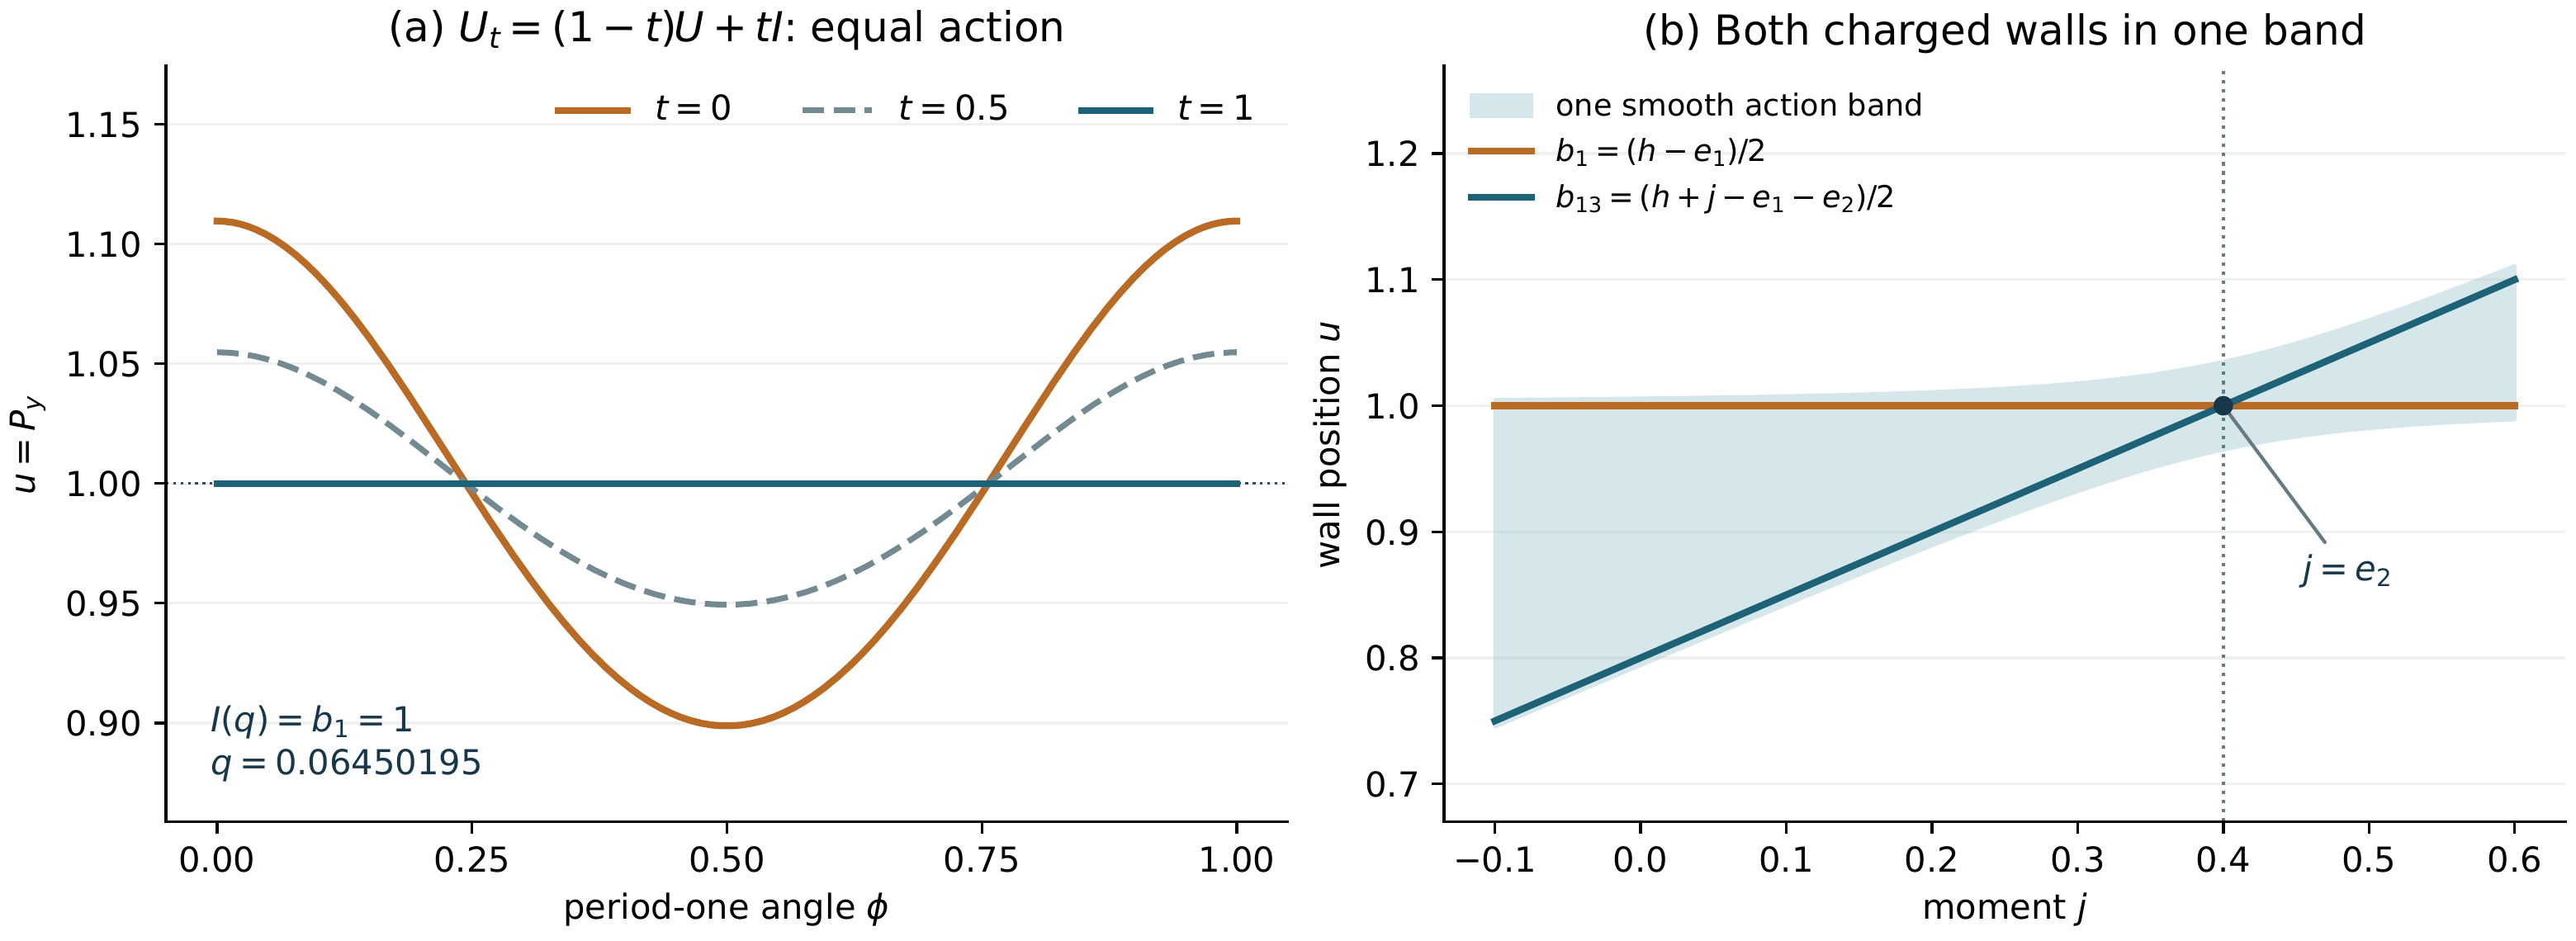
\includegraphics[width=\textwidth]{wall_straightening_geometry.png}
\caption{作用を保つ整形と二壁の同時処理。
(a) $h=3,j=0,c=0.02,e_1=1$ に対し、$I(q)=b_1=1$ を満たす
level graph を、その平均を変えず水平な円へ動かす。
(b) 同じ $h,c,e_1$ と $e_2=0.4$ について、二つの wall positions を
一つの smooth band に入れる。$j=e_2$ での一致でも band は滑らかである。
数値図は定理\ref{we:straightening}の構成を示すもので、存在証明は本文による。}
\label{we:figure}
\end{figure}

\subsection{Chosen resolved family 上の actual extension}

正の実 parameter $\tau>0$ に沿って考える。
Exact radial map $\Phi_\tau$ により $\psi_t$ を $\Omega_\tau$ 上の Hamiltonian isotopy へ運び、
\[
 (H_\tau,J_\tau,Q_\tau^\natural)
 =(H,J,Q^\natural)\circ\Phi_\tau
\]
とする。Whole focus end と whole saddle neighborhood は元の actual fibers のままである。

Central extension には isotopy 自体を $\tau=0$ へ延ばす必要はない。
まず標準空間上の一つの smooth function $Q^\natural$ を作っている。
これは $H,J$ invariant であり、修正領域では $G(H,J,u,\phi)$ と書ける。
修正の support は $P_xP_yP_z>0$ の compact regular region にあり、
wall shell では $G=\mathcal Q(H,J,u)$ で角に依存しない。
これを以下の chart expressions と組み合わせる。

First chart $x=\tau X$ では
\[
 W=\bar Xyz\sqrt{q_X^Aq_y^Aq_z^A},
\]
\[
 q_X^A=|\tau|^2+|yz|^2+\frac{e_1}{\pi(1+|X|^2)}
                   +\frac{e_2|y|^2}{\pi(1+|Xy|^2)},\quad
 q_y^A=1+|Xz|^2+\frac{e_2|X|^2}{\pi(1+|Xy|^2)},\quad
 q_z^A=1+|Xy|^2
\]
であり、中央へ smooth に延びる。
Middle chart の $x\ne0$ では式\eqref{tp:Bmap}を使う。
Last chart $(x,y,U,w)$ では $t=xyU=\tau>0$ より
\begin{equation}\label{we:last-chart}
 W=\frac{\bar x}{x}\,w\,\frac{\sqrt{P_xP_y(1+|U|^2)}}{\pi}
\end{equation}
となる。この式は $x\ne0$ で $y=U=0$ の weight-zero wall にも smooth に延びる。
$P_y$ は正の項 $e_2/(1+|U|^2)$ を含む。

残る charged walls の近傍では $\mathcal Q(H,J,P_y)$ を用いる。
Full moments $P_i$ 自体は resolved total space 上で smooth なので、
この式は collapse locus へ smooth に延びる。
他の領域では chart expressions と $G$ の smoothness を用いる。
Local ambient extensions を partition of unity で貼れば、
real-ray family 上の同じ function の smooth extension が得られる。
$H,J$ の torus で平均化した partition を使える。
Central components 上の Poisson commutativity は smooth limit、または torus invariance による。

\begin{theorem}[Relative wall filling]\label{we:actual-filling}
式\eqref{we:onewall-gap}または二壁版\eqref{we:twowall-gap}の
compact open-window hypotheses の下で、chosen graph Kähler family 上に相対変更が存在し、
次を満たす。
\begin{enumerate}
\item 非零 slice では旧 system と exact Hamiltonian 同値であり、
 protected whole focus end と whole saddle neighborhood は点ごとに固定する。
\item 選んだ walls の full neighborhoods で toric であり、
 正実 $\tau$-ray に沿って両中央 components とその共通 divisor へ滑らかに延びる。
\item Central wall は primitive circle の ordinary elliptic collapse である。
 二つの charged walls が会う free-toric-stratum の seam では、
 primitive rank-two subtorus の collapse による elliptic--elliptic toric corner を得る。
\item Protected compact block の connected-fiber quotient は非零 slice で変更されない。
 既存の $D^2\times Y$ branching と compact focus end は保たれる。
\end{enumerate}
\end{theorem}

Compact block は第\ref{ai:compact-block}項と同じ lower/upper-leg 選択で取れる。
広い parameter window では upper boundary を $q_+(h,j)=F(h,j)^2+c^2$ とすれば、
$q_s<q_+<(F+c)^2$ が自動的に成り立つ。
Lower cutoff は $q_-<c^2$、upper-leg cutoff は $c^2<q_*<\min_Rq_s$ とする。
Straightening の support は lower regular annulus 内なので、
この compact block とその connected fibers を Hamiltonian conjugacy で追える。
$H,J$ faces を点ごとに固定する optional parameter cutoff を使った場合、
中央への全 wall extension は内側の parameter rectangle についての主張である。

\paragraph{Primitive と residue.}
Foliation の wall extension は、logarithmic primitive の smooth extension を意味しない。
Middle chart の nonzero slice では
\[
 \lambda_\tau=M_1d\theta_x+P_y d\theta_Y+P_zd\theta_z
\]
であり、中央 $D_j$ 側では $M_1=e_1+\rho_x$ となる。
従って $e_1d\theta_x$ の period は残る。
Hamiltonian 修正は primitive を exact form だけ変えるため、この residue を消さない。
Normal actions $M_1-e_1$ と $e_1-M_1$ は反対符号で接ぐが、
primitive の滑らかな延長とは別の主張である。

\paragraph{未処理の core.}
本定理の wall window は $P_xP_yP_z>0$ にある。
特に middle exceptional curve の locus
\[
 P_z=0,\qquad h=e_1+2j,\qquad 0\le j\le e_2
\]
には適用していない。そこでは wall と lower pole が衝突し、
regular-annulus straightening の前提が失われる。
第一の exceptional curve の $P_y=P_z=0,\ 0\le H\le e_1$ も本 window の外である。
従って全 exceptional chain の core の充填、全 artificial boundary の除去、
任意の global form と全 geometric corner faces の同時保持は依然として別の課題である。
今回完成したのは、whole focus end と true branch を保ったまま、
その間の actual regular component walls を通す相対 filling である。

\section{残る正則 ports の actions と相対 cap の制約}
\label{pa:section}

本節では標準一次共役因子模型
\[
 H=\rho_x+\rho_y,\qquad J=\rho_y-\rho_z,
 \qquad W=\bar x yz,\qquad Q=|W-c|^2
\]
の residual ports を扱う。角度は周期1、$\rho_v=\pi|v|^2$ とする。
$(h,j)$ の compact rectangle $R$ と cut values は第\ref{ai:section}節の通り、
\[
 F(h,j)>2c,\qquad c^2<q_*<\min_R q_s,
 \qquad \max_R q_s<q_+<\min_R q_M,
\]
\[
 q_s=(F-c)^2,\qquad q_M=(F+c)^2
\]
を満たすものとする。$R$ は $j=0$ を横切る。
議論の対象は upper leg の $Q=q_*$ と merged leg の $Q=q_+$ である。

\subsection{二つの sheets と regular period lattice}

$u=\rho_y$, $L=\max(0,j)$ とすれば
\[
 f_{h,j}(u)=\frac{\sqrt{(h-u)u(u-j)}}{\pi^{3/2}},
 \qquad L\le u\le h.
\]
$u_1$ を唯一の maximum point とし、$0<R_W<F$ に対する二つの roots を
$u_-(h,j,R_W)<u_1<u_+(h,j,R_W)$ と書く。
ここでは radius を $R_W$ と記し、parameter rectangle $R$ と区別する。

$x,y,z\ne0$ 上で
\[
 \alpha=\theta_x,\qquad \beta=-\theta_z,\qquad
 \phi=-\theta_x+\theta_y+\theta_z
\]
と置くと、厳密に
\begin{equation}\label{pa:primitive}
 \lambda=h\,d\alpha+j\,d\beta+u\,d\phi,
 \qquad \arg W=2\pi\phi.
\end{equation}
$\alpha,\beta$ の orbit cycles を $\gamma_H,\gamma_J$ とする。
$|W-c|=\sqrt q$ を counterclockwise に回り、$\alpha,\beta$ を固定する
lower/upper cycles を $\gamma_-,\gamma_+$ とする。
$q\ne c^2$, $0<q<q_s$ ではこれらはそれぞれの regular fiber 上で well-defined であり、
\begin{equation}\label{pa:raw-actions}
 I_\pm(h,j,q)=\frac1{2\pi}
 \int_{|W-c|=\sqrt q}u_\pm(h,j,|W|)\,d\arg W
\end{equation}
がその primitive integrals である。
各 fiber の period lattice は
\begin{equation}\label{pa:period-lattice}
 \Lambda_\pm=\ZZ\,dh+\ZZ\,dj+\ZZ\,dI_\pm
\end{equation}
である。これは full Hamiltonian period covectors の lattice であり、
$Q$-flow の return を閉じる $H,J$-flow の補正も $dI_\pm$ に含めている。
特に marked cycle $\gamma_\pm$ の向きに沿う transverse return の二つの holonomies は
$-\partial_h I_\pm,-\partial_j I_\pm$ modulo $\ZZ$ である。
ここで lower の counterclockwise $W$-cycle は正時間の $Q$-flow に対応し、
upper の同じ向きの cycle は負時間の $Q$-flow に対応する。
従って upper の正時間 $Q$-return を取る場合には
$\partial_h I_+,\partial_j I_+$ modulo $\ZZ$ となる。

$J=0$ を横切る port collar でも、$q_*>c^2$ なら $W$ は零を避けるため、
$u_\pm$ とこの cycle chart は smooth である。
Lower focus value 自体を横切る monodromy は、本節の regular port calculation と区別する。

\subsection{Upper port の smooth cap chart と cycle jump}

Upper hemisphere では $y,z\ne0$ である。そこで
\[
 a=\theta_y+\theta_z,\qquad \beta=-\theta_z,\qquad
 \chi=\theta_x-\theta_y-\theta_z,\qquad p=h-u=\rho_x
\]
と置けば
\begin{equation}\label{pa:upper-chart}
 \lambda=h\,da+j\,d\beta+p\,d\chi,
 \qquad \xi=\sqrt{p/\pi}\,e^{2\pi i\chi}
        =x e^{-2\pi i(\theta_y+\theta_z)}.
\end{equation}
$\xi$ は $x=0$ を越して smooth であり、
\[
 W=\frac{\sqrt{(h-p)(h-j-p)}}{\pi}\,\bar\xi.
\]
従って $Q=c^2$ における $\xi=0$ は正則点である。
$Q=0$ の upper minimum は $\xi\ne0$ にあり、非退化 elliptic point である。

Upper sublevel disk $\{Q\le q\}$ の positive boundary の向きを採り、
$a,\beta$ を固定して lift した cycle を $\gamma_U$ とする。
$W$-plane 上ではこの向きは clockwise である。
この cycle とその action は $q=c^2$ を越して smooth に続く。

\begin{proposition}[Upper action と chart transition]\label{pa:upper-action}
$0<q<q_s$ に対し
\begin{equation}\label{pa:B}
 B(h,j,q):=\int_{\gamma_U}\lambda
 =\frac1{2\pi}\int_{|W-c|=\sqrt q}^{\mathrm{CCW}}
          (h-u_+(h,j,|W|))\,d\arg W
\end{equation}
は smooth で正であり、$\partial_q B>0$、$B(h,j,0)=0$ である。
$q\ne c^2$ では、$n(q)$ を $W$-circle の原点周りの winding とすると
\begin{equation}\label{pa:transition}
 n(q)=\begin{cases}0&q<c^2,\\1&q>c^2,\end{cases}
 \qquad
 \gamma_U=n(q)\gamma_H-\gamma_+,
 \qquad B=n(q)h-I_+.
\end{equation}
従って $I_+$ は $q=c^2$ で $h$ の jump を持つ。
この jump は cycle chart の変更であり、upper fiber の特異性を意味しない。
$q=c^2$ に $I_+$ の一つの極座標表示を無理に定義することはしない。
\end{proposition}

\begin{proof}
Upper chart は $h,j$ の二つの action--angle pairs と symplectic $\xi$-plane を与える。
$Q$ の upper sublevel set は $0<q<q_s$ で smooth disk であり、
その境界を正に向けた primitive integral は disk の正の symplectic area である。
これにより positivity、strict monotonicity、$q=c^2$ での smoothness が従う。
$Q=0$ の minimum に disk が縮むので $B\to0$ である。
$\chi=-\phi$ だから、positive boundary は $W$-plane で clockwise であり、
$\int p\,d\chi$ を counterclockwise $W$-circle の積分に直すと式\eqref{pa:B}となる。

座標変換は $a=\alpha+\phi$, $\chi=-\phi$ である。
$a,\beta$ を固定した clockwise cycle では $\alpha$ が $n(q)$ 回正に回り、
$\phi$ が $n(q)$ 回負に回る。これが homology relation を与える。
Primitive を積分すれば最後の action identity を得る。
\end{proof}

この port の action basis は $(h,j,B)$ とも書ける。
$q>c^2$ では $dB=dh-dI_+$ なので、式\eqref{pa:period-lattice}と同じ integral lattice を与える。
$u_c^+$ を $f(u_c^+)=c$ の upper root とすると、minimum での expansion は
\begin{equation}\label{pa:upper-min}
 B(h,j,q)=\frac{q}{2c|f'(u_c^+)|}+O(q^2).
\end{equation}
実際、$v=u-u_c^+$、$\varphi=\arg W$ に関して
$Q=f'(u_c^+)^2v^2+c^2\varphi^2+O(3)$ であり、
reduced form は $du\wedge d\varphi/(2\pi)$ だからである。

\subsection{Merged port の action と saddle での保存則}

$q_s<q<q_M$ とする。$F>2c$ なので $q>c^2$ である。
\[
 \varphi_0=\arccos\frac{F^2+c^2-q}{2cF},
 \qquad
 R_q(\varphi)=c\cos\varphi+\sqrt{q-c^2\sin^2\varphi}
\]
と置く。$|W-c|=\sqrt q$ のうち $|W|\le F$ にある arc は
$\varphi_0\le\varphi\le2\pi-\varphi_0$ に対応する。

Merged level の、maximum を含む superlevel disk $\{Q\ge q\}$ の positive boundary を
$\alpha,\beta$ 固定で lift し、$\gamma_M$ とする。
これは upper sheet を $\varphi$ 増加向きに、lower sheet を減少向きに回る cycle である。
従って
\begin{equation}\label{pa:C}
 C(h,j,q):=\int_{\gamma_M}\lambda
 =\frac1{2\pi}\int_{\varphi_0}^{2\pi-\varphi_0}
    \bigl(u_+(h,j,R_q(\varphi))-u_-(h,j,R_q(\varphi))\bigr)\,d\varphi.
\end{equation}
$C>0$, $\partial_q C<0$, $C(h,j,q_M)=0$ であり、regular period lattice は
\[
 \Lambda_M=\ZZ\,dh+\ZZ\,dj+\ZZ\,dC.
\]
$\gamma_M$ の $\theta_x$-degree は零である。

\begin{proposition}[Saddle での integral cycle relation]\label{pa:saddle-balance}
$L_s=\lim_{q\uparrow q_s}I_-(h,j,q)$,
$B_s=\lim_{q\uparrow q_s}B(h,j,q)$,
$C_s=\lim_{q\downarrow q_s}C(h,j,q)$ と置く。
これらは finite であり、saddle fiber 上の marked cycles は
\begin{equation}\label{pa:cycle-balance}
 \gamma_M=\gamma_+-\gamma_-,\qquad
 \gamma_U=\gamma_H-\gamma_+,
 \qquad \gamma_-+\gamma_U+\gamma_M=\gamma_H
\end{equation}
を満たす。従って
\begin{equation}\label{pa:action-balance}
 L_s+B_s+C_s=h.
\end{equation}
特に $j=0$ では三つの項は全て正である。
この等式は action values の等式であり、saddle における derivatives の smoothness を意味しない。
\end{proposition}

\begin{proof}
$q\downarrow q_s$ で $\varphi_0\to0$ となり、merged cycle は
upper loop の正向きと lower loop の逆向きの和へ収束する。
$W$-circle は原点を一回囲むので、upper cap cycle の式も成り立つ。
全ての lifts は同じ toric coordinates で指定しているため、追加の $J$-cycle はない。
これらは $T^2\times(S^1\vee S^1)$ の homology における等式であり、
primitive を積分すれば式\eqref{pa:action-balance}を得る。
$j=0$ では $L_s$ は正の $u_-$ を持つ circle integral、
$B_s,C_s$ は非空の正面積領域の面積なので正である。
\end{proof}

$D=-f''(u_1)>0$ と置けば、merged elliptic endpoint で
\begin{equation}\label{pa:max-expansion}
 C(h,j,q)=\frac{q_M-q}{2\sqrt{cF(F+c)D}}+O((q_M-q)^2).
\end{equation}
これは maximum 近くで
$q_M-Q=D(F+c)(u-u_1)^2+cF(\arg W-\pi)^2+O(3)$ と展開し、
楕円 disk の reduced area を計算して得る。
従って actual collapse cycle は primitive な $\gamma_M$ である。

\subsection{Merged cut を埋める actual cap}

\begin{theorem}[同じ annular embedding による merged cap]\label{pa:actual-merged-cap}
\[
 \mathcal C_M=\{(H,J)\in R,\ Q\ge q_+\}
\]
と置く。これは compact で $x,y,z\ne0$ の中に入り、
$Q=q_+$ の whole merged fibers を境界に持つ。
内部の regular fibers は $T^3$、$Q=q_M(H,J)$ の fibers は nondegenerate rank-two elliptic $T^2$ である。
第\ref{ai:section}節の annular embedding を、$K\cup\mathcal C_M$ 全体が tube に入る scale で選べば、
その同じ写像は元の $K$ の全 fibers と primitive を変えずに、merged cut を actual に埋める。
埋めた後の connected-fiber quotient は、$Q=q_M(H,J)$ に genuine な valence-one boundary を持つ。
\end{theorem}

\begin{proof}
固定した compact $(H,J)$-range 上では $\rho_x,\rho_y,\rho_z$ が有界なので $\mathcal C_M$ は compact である。
$W=0$ なら $Q=c^2<q_+$ なので、この cap では全ての coordinates が非零である。
Compactness により $|x|$ には正の下界がある。
従って annular insertion の式は cap 全体とその開近傍で定義される。
元の $K$ と重なる collar では写像も積分も同じ式である。

Scale の条件は事前に直接確認できる。
$h\le h_{\max}$、$j\ge j_{\min}$ とすれば
\[
 \rho_x,\rho_y\le h_{\max},\qquad
 \rho_z\le h_{\max}+|j_{\min}|.
\]
Twist を二つの lines に $a,d$ と配分した挿入では
\[
 |I-b|\le s\bigl((1+|a-1|)h_{\max}
              +|d|(h_{\max}+|j_{\min}|)\bigr),
 \qquad
 |Y|^2+|Z|^2\le\frac{s}{\pi}(2h_{\max}+|j_{\min}|).
\]
この bound が所定の tube の strict bounds に入れば、同じ scale $s$ で全 cap を追加できる。
既存の任意の大きい $s$ に対し domain の拡張が自動的に可能だとは主張しない。

$Q\ge q_+>q_s$ の還元領域は maximum を含む disk であり、
その center は $u=u_1$, $\arg W=\pi$ の nondegenerate maximum である。
ここでは $T^2$-action は自由なので、lift は rank-two elliptic fiber $T^2$ となる。
Action $C$ は式\eqref{pa:max-expansion}に従って零へ縮む。
従って quotient のこの端は half interval、全 parameter family では boundary face である。
\end{proof}

この cap は一つの artificial cut を処理するが、boundary-free fibration を完成させない。
同じ $(H,J,Q)$ を保って継続する限り、$Q\le q_M(H,J)$ という実際の最大値があり、
この elliptic endpoint を正則な fiber の先へ通過させることはできない。

\subsection{Upper cap の meridian と現 tube 内での障害}

自然な upper cap を
\[
 \mathcal C_U=\{(H,J)\in R,\ Q\le q_*,\ u\ge u_1(H,J)\}
\]
とする。$q_*<q_s$ のため cut $u=u_1$ は cap と交わらず、
これは upper chart の $T^2$-family of disks である。
$x=0$ は $Q=c^2$ の正則 fiber 上に現れ、cap は最後に $Q=0$ の elliptic $T^2$ へ縮む。

\begin{proposition}[Upper port の tube 内 meridian 障害]\label{pa:meridian-obstruction}
$q_*>c^2$ の upper boundary にある $\gamma_U$ は、
annular insertion 後の tube の $\theta$-circle に degree $1$ で射影する。
従って、この指定された boundary inclusion を保ちながら、
$\gamma_U$ が disk を bound する upper cap を同じ annular tube 内に埋めることはできない。
これは symplectic form や primitive の選択によらない topological obstruction である。
\end{proposition}

\begin{proof}
式\eqref{pa:transition}で $n(q_*)=1$ であり、
$\gamma_H$ の $\theta_x$-degree は1、$\gamma_+$ の degree は0である。
Annular insertion は $\theta=\theta_x$ を保つので、像の degree も1である。
Tube は annulus へ deformation retract し、$d\theta$ はその $H^1$ の generator を表す。
もし $\gamma_U$ が tube 内の disk の境界なら、closed form $d\theta$ の積分は零となり、矛盾する。
\end{proof}

同じ議論は、tube を全 $\bar C_{56}$ の normal neighborhood へ拡大しても、
対応する boundary circle が $H_1(\bar C_{56};\ZZ)$ で非零である限り成立する。
$n=24$ の各 individual boundary class は非零である。
従って各 upper port を個別の meridian disk で閉じるには、現在の curve neighborhood の外へ出る必要がある。
複数の ports をまとめて別の cobordism で接ぐ可能性は、この命題では排除しない。

\subsection{Upper cap の primitive と変更可能な面積}

Insertion の pullback primitive は $s\lambda+b\,d\theta_x$ である。
Upper chart では $\theta_x=a+\chi$ なので
\begin{equation}\label{pa:shifted-upper}
 s\lambda+b\,d\theta_x
 =(sh+b)da+sj\,d\beta+(sp+b)d\chi.
\end{equation}
Upper boundary の collapsing cycle の action は
\[
 B_{\rm out}=b+sB(h,j,q_*).
\]

\begin{proposition}[自然な cap への marked primitive extension]\label{pa:primitive-obstruction}
自然な upper cap に symplectic form $s\omega_0$ をそのまま入れる場合、
式\eqref{pa:shifted-upper}の boundary primitive が smooth に延長するためには $b=0$ が必要であり、
$b=0$ なら $s\lambda$ がその延長を与える。
この条件は、cap の形式も変えてよい任意の symplectic filling を排除する条件ではない。
\end{proposition}

\begin{proof}
同じ $s\omega_0$ の二つの primitive の差は closed である。
$\gamma_U$ は自然な cap の disk を bound するため、その差の積分は零でなければならない。
Boundary で差は $b\,d\theta_x$ なので、その積分は $b$ である。
これにより必要性が従い、十分性は明らかである。
また式\eqref{pa:shifted-upper}における $b\,d\chi$ は $p=0$ に residue $b$ を持ち、
smooth primitive としてそのまま延長することはできない。
\end{proof}

\begin{proposition}[内側の形式を変更する具体的な upper cap]\label{pa:modified-cap}
$b\ge0$ とする。Outer upper-port collar の fibers と primitive を厳密に保つ
abstract symplectic cap を、内側だけの form modification により構成できる。
その $Q=c^2$ の fibers は正則であり、最後は $Q=0$ の elliptic $T^2$ となる。
この abstract cap を現在の annular tube に埋め込む結論は含まない。
\end{proposition}

\begin{proof}
Upper boundary の $p$ の最小値は、$q_*>c^2$ と compactness により正である。
その一様な下界より小さい $\delta>0$ を選ぶ。
$\eta(p)$ を、$p$ の原点近傍で0、$p\ge\delta$ で1、$\eta'\ge0$ となる smooth function とする。
\begin{equation}\label{pa:cap-primitive}
 \lambda_b=(sh+b)da+sj\,d\beta+(sp+b\eta(p))d\chi
\end{equation}
と置く。原点近傍では最後の項は $sp\,d\chi$ なので smooth であり、
\[
 d\lambda_b=s\,dh\wedge da+s\,dj\wedge d\beta
              +(s+b\eta'(p))\,dp\wedge d\chi
\]
は $b\ge0$ により symplectic である。
Outer collar では $\eta=1$ なので式\eqref{pa:shifted-upper}と文字通り一致する。

$H,J,Q$ は $a,\beta$ に依存しないため、二つの torus moments と $Q$ の可換性は保たれる。
$Q$ の level sets は元と同じであり、正則性・elliptic minimum も保たれる。
この変更で upper disk の area は $b$ だけ増え、outer action は所定の $b+sB$ となる。
既存 insertion の boundary labels を文字通り保つには、
target integrals を $(sh,sj,s^3Q)$ と取る。
最初の二つは period-one fields $\partial_a,\partial_\beta$ を生成し、
primitive actions はそれぞれ $sh+b,sj$ である。
Hamiltonian の定数項と primitive の action を区別すれば、
元の boundary labels と marked periods の双方が一致する。
\end{proof}

対向領域への実際の埋込みには、$\gamma_U$ がそこで disk を bound することと、
この area・period lattice を許すことが必要である。
現在の annular tube は第一の条件を満たさない。
Residue を許す logarithmic primitive や異なる symplectic area を採用する比較と、
指定された smooth primitive をそのまま延長する比較を混同してはいけない。

\subsection{Upper port と merged port の単純な相対自己接着への障害}

\begin{theorem}[二つの residual ports の marked exact obstruction]\label{pa:self-gluing}
$H,J$ の functions と period-one cycles を固定し、primitive を exact term を除いて保つものとする。
同じ block の upper cut $q=q_*$ と merged cut $q=q_+$ を、
二つの interior collars が反対側になるように fiber-preserving に直接接ぐことはできない。
この主張は $j=0$ を含む parameter neighborhood で成立する。
Annular insertion の shifted primitive でも、$b\ge0$ なら同じ結論が成り立つ。
\end{theorem}

\begin{proof}
Upper interior $q>q_*$ に向かうと $B$ は増加する。
Merged interior $q<q_+$ に向かうと $C$ も増加する。
従って反対側の collars を symplectic に接ぐには、complementary cycle の向きを反転する必要がある。
$\gamma_H,\gamma_J$ を固定する integral homology isomorphism は、第三の cycle を
\[
 \gamma_U\longmapsto-\gamma_M+m\gamma_H+n\gamma_J,\qquad m,n\in\ZZ
\]
と送る。Primitive periods を保存するための必要条件は
\begin{equation}\label{pa:gluing-period}
 B(h,j,q_*)+C(h,j,q_+)=mh+nj
\end{equation}
である。$m,n$ は connected parameter neighborhood で一定である。

$j=0$ で、strict monotonicity と式\eqref{pa:action-balance}から
\[
 0<B(h,0,q_*)+C(h,0,q_+)
  <B_s+C_s=h-L_s<h.
\]
これは $mh$ と一致しないので矛盾する。

Insertion 後の periods は $A_H=b+sh$, $A_J=sj$,
$A_U=b+sB$, $A_M=sC$ である。
従って必要条件は $b+s(B+C)=m(b+sh)+nsj$ になる。
$b\ge0$ のとき $j=0$ で
\[
 0<b+s(B+C)<b+sh,
\]
なので再び整数倍と一致しない。
\end{proof}

この障害は、$H,J$ の marking、同じ二つの cuts、指定 primitive を保つ直接の接着に関するものである。
別の対向 block、異なる moment identification、追加の singular cobordism、
primitive の非 exact な変更まで排除するものではない。
しかし、両方の境界 fiber が単に $T^3$ であるという理由だけで residual ports を対向接着することはできず、
式\eqref{pa:gluing-period}の full action data が必要である。

\section{同じ二つの作用を保つ corner 充填の限界}
\label{cf:section}

第\ref{ai:section}節の annular block は whole focus fiber と whole saddle fiber を含むが、
その三つの人工的な端を閉じたわけではない。
本節では、一次共役因子模型をそのまま延長する場合に、何を埋められ、何が必ず残るかを調べる。
結論は二種類ある。固定した二つの moments の還元球面を埋めると極値が不可避であり、
また、既存 annular embedding のままでは欠けた upper cap を同じ annular tube 内に埋められない。
後者には marked primitive に関する独立の面積条件もある。
これらは、指定した $T^2$、自然な upper meridian、あるいは指定 primitive を保つ方式への制約であり、
一般の Lagrangian fibration の非存在定理ではない。

\subsection{還元球面と三つの cap}

標準 $\CC^3$ 上で
\[
 H_0=\rho_x+\rho_y,\qquad J_0=\rho_y-\rho_z,
 \qquad W_0=\bar x yz,\qquad Q_0=|W_0-c|^2,
 \quad \rho_v=\pi|v|^2
\]
と置く。角度は周期 $1$、$c>0$ とする。
$R$, $q_-$, $q_*$, $q_+$, $K$ は式\eqref{ai:q-window}--\eqref{ai:K}のものとし、
$R$ は $j=0$ を横切り、$h>\max(0,j)$、$F_1(h,j)>2c$ を満たす。
$\mu=(H_0,J_0)$、$E_{h,j}=\mu^{-1}(h,j)$ と書く。

\begin{lemma}[球面還元と面積]\label{cf:sphere}
$j\ne0$ なら、$T^2$ は $E_{h,j}$ 上で free に作用し、
\[
 \Sigma_{h,j}=E_{h,j}/T^2\simeq S^2,\qquad
 \operatorname{Area}(\Sigma_{h,j})=h-\max(0,j).
\]
内部の座標を $u=\rho_y$、$\phi=-\theta_x+\theta_y+\theta_z$ とすれば
\[
 \max(0,j)<u<h,\qquad
 \omega_{\rm red}=du\wedge d\phi,\qquad
 W_0=f_{h,j}(u)e^{2\pi i\phi},\quad
 f_{h,j}(u)=\frac{\sqrt{(h-u)u(u-j)}}{\pi^{3/2}}.
\]
また、滑らかな多様体として
\[
 E_{h,j}\simeq
 \begin{cases}
 S^3_{(x,y)}\times S^1_{\theta_z},&j<0,\\
 S^3_{(x,z)}\times S^1_{\theta_y},&j>0.
 \end{cases}
\]
第一の場合には $H_0$-orbit、第二の場合には $(H_0-J_0)$-orbit が $E_{h,j}$ 内で収縮する。
\end{lemma}

\begin{proof}
$\rho_x=h-u$、$\rho_z=u-j$ である。
内部では action の weights $(1,0),(1,1),(0,-1)$ の任意の二つが lattice basis となる。
$j\ne0$ の下極では $y,z$ のうち一方だけが零で、上極では $x$ だけが零であるから、
極でも action は free である。
Cylinder の両端の invariant angle がそれぞれ一点に潰れ、還元は滑らかな球面となる。
Moment level に制限した form は
\[
 -du\wedge d\theta_x+du\wedge d\theta_y+du\wedge d\theta_z
 =du\wedge d\phi
\]
であり、面積の式も従う。

$j<0$ では $\rho_x+\rho_y=h$ が $S^3$ を与え、
$z=\sqrt{(\rho_y-j)/\pi}\,e^{2\pi i\theta_z}$ の phase は全域で定義される。
$H_0$-orbit はこの $S^3$ の Hopf circle と一点との積である。
$j>0$ では $\rho_x+\rho_z=h-j$、$\rho_y=\rho_z+j>0$ を使えば同様で、
$H_0-J_0$ の weights は $(1,0,1)$ となる。
$S^3$ は単連結なので、記載した circles は収縮する。
\end{proof}

$P_{h,j}=(K\cap E_{h,j})/T^2$ と置く。
以下でいう cap は、$P_{h,j}$ をこの同じ $\Sigma_{h,j}$ に戻すときの補集合の closed disk を意味する。

\begin{proposition}[明示的な充填と残る極値]\label{cf:three-caps}
$j\ne0$ なら $P_{h,j}$ は pair of pants である。
その補集合は、lower sheet の $Q_0<q_-$、upper sheet の $Q_0<q_*$、
maximum 側の $Q_0>q_+$ に対応する三つの開円板である。

従って、同じ模型の全 moment box
\[
 \widehat K=\mu^{-1}(R)
\]
は $K$ を含む compact な明示的充填を与える。
ただしこの充填は、各 regular moment pair $(h,j)$ 上に二つの transverse elliptic minima と
一つの transverse elliptic maximum を含む。
それぞれの singular fiber component は $T^2$ であり、connected-fiber quotient に真の境界を作る。
残る特異点は既存の smooth saddle と、$j=0$ の lower focus locus である。
この $R$ では $y,z$-axes と原点には達していない。

より一般に、$\Sigma_{h,j}$ 上の任意の smooth function $\widetilde Q$ が
$P_{h,j}$ の三つの boundary collars で $Q_0$ と一致すれば、三つの cap の内部にそれぞれ極値を持つ。
最初の二つは極小、第三は極大である。
従って全 singularities を nondegenerate とする充填では、少なくとも三つの elliptic strata が必要である。
退化を許せば極値を退化させることはできるが、極値そのものは消せない。
\end{proposition}

\begin{proof}
$f_{h,j}$ は両端で零、内部でただ一つの strict maximum $F_1$ を持つ。
各 hemisphere は $W_0$ によって closed disk $|W_0|\le F_1$ に写る。
$F_1>2c$ の下では、$Q_0$ は $W_0=c$ に二つの minima、
$u=u_1,\phi=0$ に saddle、$u=u_1,\phi=1/2$ に maximum を持つ。
その値は順に $0,(F_1-c)^2,(F_1+c)^2$ である。
下極・上極では $W_0$ が smooth local coordinate なので $Q_0=c^2$ は regular である。
切断値の不等式から、三つの補円板と pair of pants の記述が従う。

Minima では、$(u,\phi)$ Hessian の対角項は
$2(f')^2$ と $8\pi^2c^2$ で、共に正である。
Maximum では $2f''(u_1)(F_1+c)$ と $-8\pi^2cF_1$ で、共に負である。
Free $T^2$-reduction の一点の極値を lift すると rank-two elliptic orbit $T^2$ となり、
近傍の connected-fiber quotient は $\RR^2\times[0,\varepsilon)$ 型となる。
Nondegenerate な極値の fiber component はこの orbit 自身なので、
離れた同値の fiber がその局所的な境界を消すことはない。
$\widehat K$ の compactness は $H_0$ の上界と $J_0$ の下界から従う。
$j=0$ では lower pole に既存の focus orbit が現れるが、三つの極値はその点を避ける。

任意の $\widetilde Q$ については、各 min cap の境界上の値は一定で、
cap 内側の collar ではその値より小さい。
従って compact disk 上の minimum は内部にある。
Max cap では同じ議論を $-\widetilde Q$ に適用する。
全 critical points が Morse なら、同じ結論は
$\#\mathrm{min}-\#\mathrm{saddle}+\#\mathrm{max}=\chi(S^2)=2$ とも整合する。
特に既存の一つの saddle を保持する限り、極値の数は少なくとも三つである。
\end{proof}

この命題は shared $T^2$ の regular reduction を同じ球面へ閉じる場合の制約である。
第三の関数を wall 近くで変形して central collapse に不変にする操作とは両立する。
第\ref{we:section}節の Hamiltonian 整形は三つの cap collars で恒等であり、
同じ極値の議論が $Q^\natural$ にも適用される。
その変形が focus と saddle の近傍を保っても、compact な還元球面の極値を全て除くことはできない。
他方、還元面の位相を変える接続、作用を別の場所で切り替える操作、
あるいは既存 cap meridian を変更する接続は、ここで比較した同じ充填ではない。

\paragraph{Chosen graph form への適用.}
命題\ref{tp:radial}の exact symplectomorphism $\Phi_\tau$ を用いれば、
$\tau\ne0$ の chosen K\"ahler slice 内に $\Phi_\tau^{-1}(\widehat K)$ をそのまま置ける。
これは $\Phi_\tau^{-1}(K)$ の genuine な相対充填であるが、上記の elliptic strata を持つ。
また全 reduced sphere の充填と、原点・exceptional chain・他の component regions を含む
幾何学的 corner 全体の充填とは異なる。
任意の actual curve collar に先に挿入した $K$ について、同じ相対同定が延びるとは主張しない。

\subsection{Whole moment level から見た tube obstruction}

Upper meridian 自体の annular tube 内での収縮不能性は
命題\ref{pa:meridian-obstruction}で示される。
同じ障害を full moment level の topology からも確認できる。
Distributed annular embedding は $\theta=\theta_x$ を保つので、
$j<0$ では $K$ 内の $H_0$-orbit の target $\theta$-degree が $1$ である。
一方、それは補題\ref{cf:sphere}の $E_{h,j}\simeq S^3\times S^1$ 内では収縮する。
従って $K\cap E_{h,j}$ の map は、whole $E_{h,j}$ から同じ annular tube への
continuous map にすら延長できない。
$j>0$ なら $H_0-J_0$ の orbit で同じ証明が成り立つ。
これは $a,d,b,s$ の値によらず、symplectic extension より弱い continuous extension への障害である。

より一般に、tube を含む $X$ において $[d\theta]\in H^1(\mathcal T;\ZZ)$ が
$H^1(X;\ZZ)$ の class の制限であるなら、同じ相対延長は $X$ 内でも不可能である。
必要な disk の境界に対する class の評価が、零であると同時に $1$ になるからである。
従って artificial upper face の除去には、tube の外でその一次ホモロジーを実際に殺す領域が必要である。
Contractible な actual corner chart はこの位相的条件を満たし得るが、
それだけで fibration と primitive の相対一致が得られるわけではない。

\subsection{Upper cap action の一様な上界}

以下では第\ref{pa:section}節の upper action $B(h,j,q)$ と、その正向き cycle $\gamma_U$ を使う。
$\gamma_U$ は、upper chart の二つの torus angles を固定し、
upper sublevel disk の boundary を正に向けた meridian である。
$q_*>c^2$ では $\theta_x$-degree が $1$ となる。

\begin{lemma}[Upper disk の面積上界]\label{cf:cap-area-bound}
$j=0$ とし、$c^2<q_*<(F_1(h,0)-c)^2$ とする。このとき
\[
 0<B(h,0,q_*)<\frac h3.
\]
\end{lemma}

\begin{proof}
Upper chart の reduced symplectic coordinate は
$\xi=\sqrt{p/\pi}e^{2\pi i\chi}$、$p=\rho_x=h-u$ である。
$j=0$ の radial maximum は $u_1=2h/3$ にあり、
upper hemisphere の内部は $0\le p<h/3$ という standard $\xi$-disk になる。
$q_*<(F_1-c)^2$ なので $|W-c|^2\le q_*$ の whole upper sublevel disk は
この hemisphere の内部に compact に含まれる。
$B$ はその正の symplectic area であるから、full hemisphere の面積 $h/3$ より真に小さい。
\end{proof}

Insertion 後の upper-meridian period は、命題\ref{pa:upper-action}と
式\eqref{pa:shifted-upper}により
\[
 P=b+sB(h,j,q_*).
\]
この oriented meridian を symplectic disk で埋め、所定 primitive が disk 全体へ
smooth に延びるなら、Stokes によって disk の必要面積はちょうど $P>0$ である。
同じ scaled standard cap の場合は $b=0$ が必要である
（命題\ref{pa:primitive-obstruction}）。
以下では、cap 内部の面積を変更しても残る $P>0$ という条件を使う。

\subsection{$C_{56}$ の全24端に対する同時 cap obstruction}

定理\ref{ai:c56-allends}の global curve primitive を $\beta$ とする。
各 collar 内の center circle を選び、これらを boundary とする compact curve region を $C'$ と書く。
角 $\theta_i$ は deleted disk に対して反時計回りなので、$C'$ の boundary orientation とは逆である。
各 center circle 上で $\beta=I_i^0d\theta_i$、挿入の定数を
\[
 b_i=I_i^0-s_i h_i^0,\qquad s_i>0,\quad h_i^0>0
\]
とする。ここでは scale と prototype の longitudinal value を端ごとに変えてよい。

\begin{corollary}[24個の自然な exact caps は同時には貼れない]\label{cf:allends-obstruction}
上の marked primitives を保つと
\begin{equation}\label{cf:sum-b}
 \sum_{i=1}^{24}b_i
 =-\operatorname{Area}(C')-\sum_{i=1}^{24}s_i h_i^0<0.
\end{equation}
従って、全24端をそれぞれの同じ scaled standard upper cap で埋め、
各 cap 全体へ既存 primitive を smooth に延ばすことは不可能である。

さらに $j=0$ の自然な upper meridians を選び、
$B_i=B(h_i^0,0,q_{*,i})$、その既存 primitive periods を $P_i=s_iB_i+b_i$ とすると
\begin{equation}\label{cf:negative-cap-period}
 \sum_{i=1}^{24}P_i
 =-\operatorname{Area}(C')-\sum_{i=1}^{24}s_i(h_i^0-B_i)
 <-\operatorname{Area}(C')-\frac23\sum_{i=1}^{24}s_i h_i^0<0.
\end{equation}
少なくとも一つの $P_i$ は負である。
従って cap の内部面積を変更しても、同じ oriented meridians を symplectic disks で埋め、
全ての marked primitives を各 disk へ延ばすことはできない。
\end{corollary}

\begin{proof}
Stokes の定理と boundary orientation により
\[
 \operatorname{Area}(C')=\int_{C'}d\beta=-\sum_i I_i^0.
\]
$b_i$ の定義を代入すると式\eqref{cf:sum-b}を得る。
同じ standard caps なら命題\ref{pa:primitive-obstruction}が全ての $b_i=0$ を要求するので矛盾する。
一般の面積を許す場合も、補題\ref{cf:cap-area-bound}より $0<B_i<h_i^0/3$ であり、
period の総和を計算すると式\eqref{cf:negative-cap-period}となる。
負の period は、smooth primitive の存在下では正向き symplectic disk の boundary にはなれない。
\end{proof}

Global primitive $\beta$ を別の primitive に変えても、closed difference の全 boundary periods の和は零なので、上の総和は変わらない。

この結論が除外するのは、既存の三つの marking、すなわち
global $\beta$ から来る primitive periods、自然な upper meridians、その cap の向きを
同時に保つ方式である。
必要に応じて meridian に torus cycle を加える接着、nonexact primitive transitions、
別の shared-action model への切替えを検討する余地が残る。
特にこの系から、一般の symplectic gluing や元の大域目標の非存在を結論しない。

\subsection{Ambient cohomology が要求する cap periods の総量}

以下では、系\ref{cf:allends-obstruction}の原始形式を曲線近傍の外へそのまま延長する条件を外す。
代わりに、actual ambient class が cap 側との period differences に課す必要条件を記録する。

定理\ref{ai:c56-allends}で使った一つの global normal-neighborhood embedding の
fibrewise disk-domain の像を $N$ とする。
必要なら base の collars を少し広げ、全24個の meridians と
それらを zero section へ戻す normal radial homotopies が $N$ に入るように取る。
$N$ は punctured curve の normal disk bundle であり、$H^2(N;\RR)=0$ である。
Global $\beta$ を用いた normal-model primitive の pushforward により、
actual form について $d\lambda_N=\omega|_N$ となる一つの $\lambda_N$ を固定できる。
その collar periods は、これまで指定してきた marked periods と一致する。

$\gamma_i$ を $j=0$, $h=h_i^0$, $q=q_{*,i}$ における正向きの自然な upper meridian とし、
\[
 P_i=\int_{\gamma_i}\lambda_N=b_i+s_iB_i
\]
と置く。
Global normal model での base projection は
$\widehat I_i=b_i+s_iH_0=I_i^0$、$\theta_i=\theta_x$ なので、
$\gamma_i$ は centre circle $\ell_i$ の反時計回りの class に写る。
従って、$\partial C'=-\sum_i\ell_i$ という向きの規約の下で
\[
 \sum_{i=1}^{24}[\gamma_i]=0\qquad\text{in }H_1(N;\ZZ).
\]
これは integral な関係である。Normal radial homotopies と $C'$ を用いて、
$\partial S=-\sum_i\gamma_i$ となる integral smooth singular $2$-chain $S\subset N$ を取れる。

\begin{corollary}[自然な caps に必要な ambient period budget]
\label{cf:ambient-period-budget}
Actual compact symplectic manifold $X_d$ の class が
\[
 [\omega]=aH,\qquad a>0,\qquad H=c_1(\mathcal O_{X_d}(1))\in H^2(X_d;\ZZ)
\]
であるとする。各 $\gamma_i$ が $X_d$ 内の oriented symplectic disk $D_i$ の境界となり、
$\partial D_i=\gamma_i$ と正向きで一致すると仮定する。
Disks が互いに素であることは仮定しない。
$A_i=\int_{D_i}\omega>0$ と置くと、ある $n\in\ZZ_{>0}$ に対して
\begin{equation}\label{cf:ambient-budget}
 \sum_{i=1}^{24}(A_i-P_i)=a n
\end{equation}
が必要である。さらに
\begin{equation}\label{cf:ambient-budget-bound}
 a n>
 \sum_{i=1}^{24}A_i+\operatorname{Area}(C')
       +\frac23\sum_{i=1}^{24}s_i h_i^0.
\end{equation}

各 cap の近傍で primitive $\lambda_i$ を選び、
$r_i=\int_{\gamma_i}(\lambda_i-\lambda_N)=A_i-P_i$ と書けば、
$\sum_i r_i=a n$ である。
従って個別の $r_i$ ではなく、その総和が ambient period group $a\ZZ$ に属し、
この場合には正でなければならない。
\end{corollary}

\begin{proof}
上の $S$ に Stokes を適用すると
\[
 \int_S\omega=\int_{\partial S}\lambda_N=-\sum_iP_i.
\]
従って $Z=\sum_iD_i+S$ は closed integral $2$-cycle であり、
\[
 \int_Z\omega=\sum_i A_i-\sum_iP_i
       =a\langle H,[Z]\rangle.
\]
$n=\langle H,[Z]\rangle\in\ZZ$ と置く。
式\eqref{cf:negative-cap-period}と $A_i>0$ により左辺は正で、
さらに式\eqref{cf:ambient-budget-bound}の strict lower bound を持つ。
従って $n>0$ である。
各 $\lambda_i$ については disk 上の Stokes により
$\int_{\gamma_i}\lambda_i=A_i$ なので、最後の表示も従う。
$S$ を別の chain に変えても、その差は exact な $N$ 内の closed cycle であるため
$\omega$-period は零であり、$n$ は変わらない。
\end{proof}

ここで固定しているのは $N$ 上の $\lambda_N$ であり、
$N\cup\bigcup_iD_i$ 全体に同じ primitive が延びるとは仮定していない。
そのような延長があれば全ての $r_i$ が零となり、上の正の総量に反する。
同様に、この union を一つの exact symplectic region に収めることもできない。
また $Z$ は積分 cycle であって、embedded symplectic surface としての存在を主張するものではない。
本系は仮定した disks の面積と cohomology に対する必要条件であり、
それらの disks、相対 cap fibrations、または大域 completion の存在を与えない。

\subsection{還元の exactness と focus monodromy を区別する}

$\omega_0=d\lambda_0$ であることは、還元球面の form が exact であることを意味しない。
実際 $\lambda_0(X_{H_0})=h$、$\lambda_0(X_{J_0})=j$ なので、
$\lambda_0|_{E_{h,j}}$ は basic ではない。
Period-one connection forms $\alpha_H,\alpha_J$ を取り、
$\int_{\Sigma}d\alpha_H$、$\int_{\Sigma}d\alpha_J$ を curvature numbers と呼ぶ規約では
\begin{equation}\label{cf:curvature-vectors}
 (e_H,e_J)=
 \begin{cases}(1,0),&j<0,\\(1,-1),&j>0,\end{cases}
 \qquad
 [\omega_{\rm red}]=h[d\alpha_H]+j[d\alpha_J].
\end{equation}
従って sphere area はそれぞれ $h$、$h-j$ となり、補題\ref{cf:sphere}と一致する。

この curvature 計算は直接できる。
$j<0$ では $(x,e^{2\pi i\theta_z}y)\in S^3$ の Hopf connection を $\alpha_H$、
$-d\theta_z$ を $\alpha_J$ とすればよい。
$j>0$ では $(x,e^{2\pi i\theta_y}z)\in S^3$ の Hopf connection を $\alpha_H$、
$d\theta_y-\alpha_H$ を $\alpha_J$ とする。
いずれも $\alpha_r(X_s)=\delta_{rs}$ を満たし、正向きの Hopf curvature の積分は $1$ である。
一般に $\lambda_0-h\alpha_H-j\alpha_J$ の basic な部分を微分すれば、
式\eqref{cf:curvature-vectors}の cohomology identity が得られる。
従って正の面積を持つ reduced sphere と ambient exactness との間に矛盾はない。
一方、sphere 全体に reduced primitive を要求すれば Stokes に反する。

Lower focus の小さい transverse loop における fiber monodromy は、
longitudinal cycle $\Gamma_H$ と vanishing cycle $\Gamma_J$ を固定し、
第三の cycle $\delta$ を
\[
 \delta\longmapsto\delta+\Gamma_J
\]
へ移すように transverse loop の向きを選ぶ。Loop の向きを逆にすれば符号は逆になる。
これは単一 focus point の標準 monodromy である\cite[\S3, Lemma 1]{zung-focus-cf}。
上の curvature vector の差 $(0,-1)$ も、この一つの vanishing circle を検出している。
Hamiltonian $T^{n-1}$ の curvature と monodromy の一般の関係については
\cite[Theorems 3.2 and 3.15]{efstathiou-martynchuk-cf} を参照。

Distributed twists の $a+d$ は normal frame に対する winding であって、
この single-focus monodromy の係数ではない。
式\eqref{ai:distributed-map}の distributed shear は対応する $H,J$ cycles を移すので、$a+d=2$ でも上の係数は $1$ である。
Focus neighborhood を固定した cap attachment や wall repair は、この小さい loop の monodromy を変えない。
従って winding の収支、primitive の収支、還元球面の極値、focus monodromy は、
それぞれ別の接着条件として追跡する必要がある。

\section{固定平面六次曲線と actual な個別 upper disks}
\label{ad:section}

本節は $t=\tau\ne0$ を固定する。
定理\ref{ai:c56-allends}の punctured curve を、元の pencil に存在する一つの閉曲線から選ぶ。
これにより自然な upper meridians を actual symplectic disks で個別に埋め、
その primitive の不足分を閉曲線の面積として計算できる。
Disk の族、cap fibration、あるいは既存積分の disk 全体への延長は主張しない。

\subsection{Punctured lift の具体的な選択と normal frames}

\begin{proposition}[固定曲線による actual lift]\label{ad:fixed-curve}
元の pencil
\[
 X_t=\left\{L_1L_2L_3L_4L_5L_6+tF_6=0\right\}\subset\PP^4
\]
に対し
\[
 C^*=\{L_5=L_6=F_6=0\}
\]
は全ての smooth $t\ne0$ の $X_t$ に含まれる同じ smooth plane sextic である。
その normal bundle と面積は
\begin{equation}\label{ad:normal-area}
 N_{C^*/X_t}\simeq\mathcal O_C(1)\oplus\mathcal O_C(1),
 \qquad \int_{C^*}H=6,\qquad \int_{C^*}\omega_t=6a
 \quad([\omega_t]=aH)
\end{equation}
である。$G=L_1L_2L_3L_4$ の零点24個を含む互いに素な小円板を削除すれば、
この punctured curve を既存 $\bar C_{56}$ の actual lift として選べる。
この選択は既存の明示的な collar family と一致する。
\end{proposition}

\begin{proof}
$L_5=L_6=0$ 上では pencil の方程式は $tF_6=0$ となる。
従って $t\ne0$ では $C^*$ は $X_t$ 内の二つの hyperplane sections の
scheme-theoretic な横断的 complete intersection である。
横断性は $F_6|_{P_5\cap P_6}$ の零曲線の smoothness から従い、
conormal sequence が normal bundle の式を与える。
Plane sextic の hyperplane degree は6なので面積の式も従う。
本稿の chosen class $aH+\eps A$ は $t\ne0$ 上では $aH$ に制限される。

各 puncture では、単元を吸収した既存の chart
\[
 xyz=tw,\qquad t=xT,\quad y=TY,\quad w=Yz
\]
を使う。$C^*_t$ の strict lift は正確に
\[
 Y=z=0,\qquad T=t/x
\]
である。これは式\eqref{sc:nonzero-chart}で用いた actual collar であり、
削除円板の外では $x\ne0$ のため $t=0$ へ smooth に延びる。
従って一般の horizontal lift を選ぶ代わりに、この固定曲線を選べばよい。
\end{proof}

Normal frames の次数差もこの同定で直接見える。
以下では順序を、$z=L_6$ 方向の $\mathcal O_C(1)$ と、
central $V_5$ の normal である $\mathcal O_C(5)$ の順とする。
元の pencil の係数で $\mathcal Y=F_6/L_6$ と書くと、$G\ne0$ 上では
\begin{equation}\label{ad:frame-comparison}
 y=L_5=-\frac{t}{G}\mathcal Y,
 \qquad
 \partial_{\mathcal Y}\longmapsto-\frac{t}{G}\partial_y
\end{equation}
が normal first jet の同定である。
ここで $\mathcal Y$ は central blow-up の $\mathcal O(5)$ 座標であり、
annular tube の $Y$ という名前と自動的には同一視しない。
式は $Gyz+tF_6=0$ を用いて $F_6/z$ を holomorphically 延長すれば得られる。
第一の $z$ 方向は変化しない。

$G|_C$ は24個の simple zeros を持つので、第二の frame comparison は
各 deleted disk の counterclockwise 境界で winding $-1$ を持つ。
従って normal degree は $(6,30)$ から $(6,6)$ へ変わる。
特に式\eqref{ai:individual-sections}の algebraic sections は
\begin{equation}\label{ad:actual-sections}
 (L_1,L_1L_2^2L_3L_4)\longmapsto(L_1,-tL_2)
\end{equation}
となる。Unitary normalization と orthogonalization はこの relative degree を変えない。
Semistable frame における determinant profile $(2,2,1,1)$ は、
actual disk frames では $(1,1,0,0)$ となる（各型6端）。
これは frame の比較であり、dual mixed Hessian の winding と向きを混同しない。

\subsection{個別の graph disks と exact な面積収支}

Actual $C^*\subset X_\tau$ 上で互いに素な閉円板 $\Delta_i$ を固定し、
その正向き境界を $c_i$、補集合を
\[
 C'=C^*\setminus\bigcup_{i=1}^{24}\operatorname{int}\Delta_i
\]
とする。各円板は対応する puncture を含み、$\partial C'=-\sum_i c_i$ である。
先に円板を十分小さく選び、
\[
 0<A_i^{\rm base}:=\int_{\Delta_i}\omega_\tau<a
\]
としてよい。以後は $\tau$、円板、collars、normal embeddings を固定する。
一つの global primitive $d\beta=\omega_\tau|_{C'}$ と既存の normal-model primitive を使い、
collars では
\[
 \beta=\widehat I_i\,d\theta_i,\qquad c_i=\{\widehat I_i=I_i^0\}
\]
とする。Actual primitive と model primitive の exact difference は periods に影響しない。

\begin{theorem}[Actual individual upper disks と次数6の budget]\label{ad:disks}
各 collar で固定した prototype parameters
\[
 H_0=h_i^0>0,\qquad J_0=0,\qquad
 c^2<q_{*,i}<(F_1(h_i^0,0)-c)^2
\]
と自然な upper meridian $\gamma_{U,i}$ を選ぶ。
Annular insertion の scale を $s_i>0$、offset を
\[
 b_i=I_i^0-s_i h_i^0
\]
とする。十分小さい scales に対し、各 actual $\gamma_{U,i}$ は
$\Delta_i$ 上の $C^1$-small normal graph である embedded symplectic disk $D_i$ を bound する。
その面積 $A_i$ と既存 primitive period $P_i$ は
\begin{align}
 P_i&=b_i+s_i B_i,\qquad B_i=B(h_i^0,0,q_{*,i}),\label{ad:period}\\
 A_i&=A_i^{\rm base}+P_i-I_i^0
     =A_i^{\rm base}-s_i(h_i^0-B_i),\label{ad:disk-area}\\
 0&<A_i<a.\nonumber
\end{align}
また、$c_i$ から $\gamma_{U,i}$ への radial normal annulus $\mathcal A_i$ を
$\partial\mathcal A_i=\gamma_{U,i}-c_i$ と向けると、closed cycle
\begin{equation}\label{ad:cycle}
 Z=C'+\sum_i(D_i-\mathcal A_i)
\end{equation}
は $[Z]=[C^*]\in H_2(X_\tau;\ZZ)$ を満たす。従って
\begin{equation}\label{ad:budget}
 \int_ZH=6,\qquad \boxed{\ \sum_{i=1}^{24}(A_i-P_i)=6a\ }.
\end{equation}
\end{theorem}

\begin{proof}
Twists を $(a_i,d_i)$ に配分した insertion を使う。
式\eqref{ai:distributed-end}の共通 curve-model coordinates では厳密に
\begin{equation}\label{ad:graph-coordinates}
 \widehat I_i=b_i+s_iH_0,\qquad
 U=\sqrt{s_i}\,e^{-2\pi i\theta_x}y,\qquad
 V=\sqrt{s_i}\,z,
 \qquad \theta_i=\theta_x.
\end{equation}
従って、ここでいう base projection は physical tube の $I$ ではなく
共通 global normal model の $\widehat I_i$ である。

自然な upper meridian では $\theta_y+\theta_z$ と $-\theta_z$ を固定するので、
$\theta_y,\theta_z$ は共に一定である。
$W=c+r e^{-2\pi i\ell}$, $r=\sqrt{q_{*,i}}>c$, と parameterize すれば
\[
 \frac{d}{d\ell}\arg W
 =-2\pi\frac{r(r+c\cos(2\pi\ell))}{|W|^2}<0.
\]
他方 $\theta_x=\theta_y+\theta_z-\arg W/(2\pi)$ だから、
$\theta_x$ は正向きに単調に一周する。
式\eqref{ad:graph-coordinates}では $\widehat I_i=I_i^0$ であり、
従って $\gamma_{U,i}$ は $c_i$ 上の normal section の graph である。
Prototype parameters と $\tau$ を固定しているため、その $C^1$ norm は $O(\sqrt{s_i})$ である。

閉曲線 $C^*$ の smooth tubular neighborhood を、選んだ compact collars 上では
既存の common normal embedding と一致するように選ぶ。
これは actual normal bundle を用いた relative tubular construction で可能である。
具体的には、二つの tubular germs の first jet を actual normal bundle で一致させ、
その差 $O(|v|^2)$ を base の cutoff で延ばせば、十分小さい radius で embedding のままである。
Disk 上では normal bundle は trivial なので、境界 section を
固定した collar extension と cutoff で $\Delta_i$ 全体へ延ばせる。
この extension の $C^1$ norm も $O(\sqrt{s_i})$ であり、中心近傍で零にしてよい。
得られる graph は positive complex disk $\Delta_i$ に $C^1$-close なので、
十分小さい $s_i$ では embedded symplectic disk となる。
Frame 自身が disk へ nonvanishing に延びる必要はなく、section は零点を持ってよい。
有限個の円板について同時に scales を小さくできる。

Radial normal annulus は既存の primitive が定義された collar tube 内にあり、Stokes により
\[
 \int_{\mathcal A_i}\omega_\tau=P_i-I_i^0.
\]
Disk の normal section を零へ縮める homotopy は
$D_i-\Delta_i-\mathcal A_i$ を境界とする3-chain を与える。
従って式\eqref{ad:disk-area}と $[Z]=[C^*]$ が従う。
補題\ref{cf:cap-area-bound}の $0<B_i<h_i^0/3$ より、
$s_i(h_i^0-B_i)<A_i^{\rm base}$ まで scale を縮めれば
$0<A_i<A_i^{\rm base}<a$ である。

最後に $\operatorname{Area}(C')=-\sum_iI_i^0$ なので
\[
 \int_Z\omega_\tau
 =\operatorname{Area}(C')+
   \sum_i\bigl(A_i-P_i+I_i^0\bigr)
 =\sum_i(A_i-P_i)=6a.
\]
これで向きと primitive constants を含む budget が得られる。
\end{proof}

\paragraph{範囲と central limit.}
この構成は各指定 cycle を埋める個別の disk を与える。
Disk 内部と既存 assembly 全体との非交差、$T^2$-family of disks、
Lagrangian cap fibration、所定の $H,J,Q$ の延長はこの定理の結論に含めない。
また既存 primitive が $D_i$ 全体へ延びるとも主張しない。
その差の総和が $6a$ であるため、式\eqref{cf:negative-cap-period}との矛盾はない。
小ささの定数は固定した $\tau\ne0$ に依存し、$\tau\to0$ の一様な radius は得ていない。

閉曲線族の central limit も、punctured lift の limit と区別する必要がある。
各 puncture の chart では $Y=z=0$, $t=xT$ なので、$t=0$ には
strict $C_{56}$ に対応する $T=0$ と、最初の blow-up の exceptional curve に対応する $x=0$ が現れる。
従って closed limit cycle は $C_{56}$ 単独ではなく、
24個の exceptional $\PP^1$ を付加したものである。
式\eqref{ad:normal-area}の閉曲線の面積を、strict $C_{56}$ の面積だけと同一視してはいけない。

\section{Actual sextic 上の upper meridian の Maslov 指数と cap 障害}
\label{mx:section}

本節は actual curve の lift を特定した構成について述べる。
Smooth fiber を
\[
 X_\tau=\{L_1L_2L_3L_4L_5L_6+\tau F_6=0\}\subset\PP^4,
 \qquad \tau\ne0,
\]
とし、smooth plane sextic
\[
 C^*=\{L_5=L_6=F_6=0\}\subset X_\tau
\]
を curve block の lift に選ぶ。
$\mathsf H=c_1(\mathcal O_{X_\tau}(1))$、$[\omega]=\mathfrak a\mathsf H$、
$\mathfrak a>0$ とする。$\mathfrak a$ は distributed twist の整数 $a$ と区別する。
24 punctures は $C^*\cap\{L_i=0\}$、$i=1,2,3,4$ の各6点であり、
全て単純かつ互いに異なると仮定する。
各 puncture の actual disk へ延びる normal frames を固定し、
annular embedding の first jet は以下の algebraic comparison と
positive-diagonal Gram--Schmidt から定める。

\subsection{Actual disk frame における一回の補正}

$C^*$ は $X_\tau$ 内で二つの hyperplanes の transverse complete intersection なので
\[
 N_{C^*/X_\tau}\simeq\mathcal O_{C^*}(1)\oplus\mathcal O_{C^*}(1).
\]
一方、central $C_{56}$ では low/high normal lines が
$\mathcal O_C(1),\mathcal O_C(5)$ である。
$G=L_1L_2L_3L_4$ と置き、$y=L_5$, $z=L_6$、
central chart の high coordinate を $Y_{\rm alg}=F_6/z$ と書く。
$G\ne0$ 上の relation は
\begin{equation}\label{mx:normal-comparison}
 y=-\frac{\tau}{G}Y_{\rm alg},\qquad
 \partial_{Y_{\rm alg}}=-\frac{\tau}{G}\partial_y
 \quad\text{along }C^*.
\end{equation}
Low normal $\partial_z$ は補正を受けない。
各 puncture の正向き circle で $G$ は winding $+1$ を持つので、
central high frame は actual disk frame に対して winding $-1$ を持つ。
これは bundle degrees の差だけからの推定ではなく、式\eqref{mx:normal-comparison}の first-jet identity である。
Nonzero local units、constant $-\tau$、positive-diagonal Gram--Schmidt は、この winding を変えない。

第\ref{ai:distributed}項の tube variables $(Y,Z)$ は low/high の順序であり、
algebraic variables $(Y_{\rm alg},z)$ の順序とは異なる。
Distributed insertion の normal factors は
\[
 Y=\sqrt s\,e^{2\pi i(a-1)\theta}y_{\rm src},\qquad
 Z=\sqrt s\,e^{2\pi id\theta}z_{\rm src},\qquad k=a+d.
\]
従って actual disk frames に関する二つの derivative factors の winding は
\begin{equation}\label{mx:normal-degrees}
 (a-1,d-1),\qquad \text{その和は }k-2.
\end{equation}
二つの normal lines を一緒に順序交換しても determinant の定数符号しか変わらない。
これは normal first jet の比較である。Full symplectic coordinate change には
base moment の $O(|v|^2)$ 補正も含まれ、それは actual tubular embedding に保持する。

Global central sections はこの comparison によって
\[
 (L_1,L_1L_2^2L_3L_4)\longmapsto(L_1,-\tau L_2)
\]
となる。Actual determinant frame の puncture windings は
$(1,1,0,0)$ 各6個であり、central の $(2,2,1,1)$ 各6個から一つずつ減る。

\subsection{Upper meridian と derivative loop}

標準模型の $h,j$ と upper regular cut
\[
 c^2<q_*<q_s(h,j)
\]
を固定する。$\gamma_U$ は第\ref{pa:section}節の positive upper meridian とする。
式\eqref{pa:upper-chart}の $a_{\rm ang}=\theta_y+\theta_z$, $\beta=-\theta_z$ を固定すると、
$\gamma_U$ の original angular degrees は
\begin{equation}\label{mx:source-angular}
 (\deg\theta_x,\deg\theta_y,\deg\theta_z)=(1,0,0).
\end{equation}
実際 $|W-c|=\sqrt{q_*}$ は原点を囲み、$\gamma_U$ はその clockwise lift である。
円の原点周りの argument は単調なので、$\theta_x$ 自体を正向き parameter にできる。

Source upper sublevel disk は、$a_{\rm ang},\beta$ を固定した smooth $\xi$-disk である。
その周上の Lagrangian tangent bundle は二つの固定された real directions と
正向き plane curve の tangent line に分解する。
従って source Cartesian trivialization に関して
\begin{equation}\label{mx:source-maslov}
 \mu_{\rm src}(\gamma_U)=2.
\end{equation}
この sign は positive symplectic disk の boundary orientation に対応する。

\begin{lemma}[Actual derivative loop の degree]\label{mx:derivative}
Actual annular embedding $\Phi_s$ の first jet を上記の通り選ぶ。
Scale $s$ は、$\gamma_U$ の source normal coordinates を零へ縮める compact homotopy
の全体が同じ annular chart に入るほど小さいとする。
Source Cartesian frames と actual disk へ延びる symplectic frames の間で、
$s^{-1/2}D\Phi_s$ の unitary polar part の determinant degree は $k-2$ である。
\end{lemma}

\begin{proof}
Normal contraction は derivative loops の homotopy を与える。
その終点の source axis では derivative は base block と二つの normal blocks に分かれる。
Base map は
\[
 (\rho_x,\theta_x)\longmapsto (b+s\rho_x,\theta_x)
\]
から actual curve annulus への orientation-preserving map である。
Disk Cartesian frames の間でその derivative loop の degree は零である。
例えば radial area coordinates では、radial map
$re^{i\vartheta}\mapsto R(r)e^{i\vartheta}$ の derivative は
$R_\vartheta\operatorname{diag}(R'(r),R(r)/r)R_{-\vartheta}$ であり、
positive-definite symmetric なので unitary polar part は恒等となる。
General disk-compatible coordinates でも、source と target の正向き simple circles の
tangent turning numbers がともに1であるため degree は零のままである。
Normal blocks の和は式\eqref{mx:normal-degrees}により $k-2$ である。
Relative Moser correction は zero section 上で first-jet identity なので、
上の contraction による degree を変えない。
Compactness と、base displacement が $O(s)$、normal size が $O(\sqrt s)$ であることにより、
必要な homotopy は scale を小さくすれば同じ chart 内で実行できる。
\end{proof}

Maslov index は unitary determinant の二乗の degree である。
従って symplectic derivative loop の determinant degree が $m$ なら、
Lagrangian loop の Maslov index への寄与は $2m$ となる。
この規約および positive plane disk の index $2$ は
\cite[\S2.3, Example 2.10, Theorem 3.1]{cho-shin-maslov}と一致する。

\subsection{Reference disk と Maslov 指数}

定理\ref{ad:disks}の actual graph disk を $D_0$ とし、
その面積を $A_0$ と書く。前節の Kähler scale $a$ は本節の $\mathfrak a$ である。
Base disks を先に $0<A_i^{\rm base}<\mathfrak a$ で選んでから insertion scales を縮めれば、
同定された actual disk neighborhood 内で
\begin{equation}\label{mx:small-area}
 0<A_0=A_i^{\rm base}-s_i(h_i^0-B_i)<\mathfrak a
\end{equation}
を満たす embedded symplectic disk がある。
この面積は global punctured-neighborhood primitive の period $P_i$ とは異なる。
既存 primitive が disk 全体へ延びることは仮定していない。

\begin{proposition}[Actual upper disk の Maslov 指数]\label{mx:index}
定理\ref{ad:disks}の $D_0$ に対して
\begin{equation}\label{mx:maslov-value}
 \mu_{L_s}(D_0)=2+2(k-2)=2k-2.
\end{equation}
従って central determinant winding $k=1$ の端では $\mu(D_0)=0$、
$k=2$ の端では $\mu(D_0)=2$ である。
\end{proposition}

\begin{proof}
Actual disk neighborhood は contractible であり、その symplectic tangent frame は
$D_0$ まで延びる。Source disk の frame も source Cartesian frame と homotopic である。
式\eqref{mx:source-maslov}と補題\ref{mx:derivative}を用いて
actual boundary Lagrangian loop の index を計算すればよい。
\end{proof}

\subsection{Primitive に依存しない12端の elliptic-cap 障害}

$X_\tau$ の tangent-normal exact sequence から
\[
 c_1(TX_\tau)=(5-6)\mathsf H=-\mathsf H
\]
となる。$D'$ が $L_s$ 上で $D_0$ と同じ oriented marked boundary class
$\gamma_U$ を持つ任意の disk とする。
Boundary representatives が異なる場合は $L_s$ 内の annulus を加えて一致させる。
$L_s$ は Lagrangian なのでこの操作は area を変えない。
$D'$ と $-D_0$ を接いだ sphere class を $A$、$n=\langle\mathsf H,A\rangle\in\ZZ$ と置けば
\begin{equation}\label{mx:sphere-comparison}
 \mu(D')=2k-2-2n,\qquad
 \int_{D'}\omega=A_0+\mathfrak a n.
\end{equation}
第一の式は relative Maslov class の sphere restriction が $2c_1$ であることによる。
例えば \cite[Definition 2.8 and Theorem 3.1]{cho-shin-maslov}の curvature formula を
二つの disks に同じ boundary connection で適用して差を取れば、
closed sphere の Chern--Weil formula のちょうど二倍になる。
$\pi_2(X_\tau)\simeq\ZZ$ などの追加の同定は必要ない。

特に $\mu(D')=2$ なら
\begin{equation}\label{mx:maslov-two-area}
 n=k-2,\qquad \int_{D'}\omega=A_0+\mathfrak a(k-2).
\end{equation}

\begin{theorem}[12 upper meridians の positive Maslov-two cap は存在しない]
\label{mx:twelve-caps}
上記の actual $C^*$ lift、specified first jets、小さい disks と scales を用いた
24端の assembly を考える。
$L_3=0$ または $L_4=0$ に属する12端の各 upper meridian $\gamma_U$ は、
$X_\tau$ のどこにおいても、positive-area Maslov-index-two disk の boundary にはならない。
従ってこの marked meridian を保ち shared $T^2$ が自由に延びる
ordinary elliptic disk cap によって、これら12 ports を埋めることはできない。
Primitive の全域への延長や exact gluing は仮定していない。
\end{theorem}

\begin{proof}
これら12端では $(a,d)=(0,1)$、$k=1$ である。
式\eqref{mx:maslov-two-area}により Maslov-two disk の area は
$A_0-\mathfrak a<0$ となり、positivity に矛盾する。

最後の帰結における ordinary elliptic disk cap は、fixed shared moments の還元が
一つの非退化 elliptic point を持つ smooth symplectic disk であり、
その positive boundary の collapsing primitive cycle が $\gamma_U$ であるものを指す。
Shared $T^2$ が自由なので、fixed-moment level の disk 上の principal $T^2$ bundle は trivial である。
Section を取ると、その pullback form は reduced symplectic form であり、
positive symplectic disk を得る。Section の boundary は elliptic point で潰れる cycle であり、
cap に指定した collapse marking によって $\gamma_U$ と同定される。
二つの noncollapsing Hamiltonian vector fields と compatible complex structure は
disk 上に延びる complex rank-two summand の frame を与え、
残る reduced tangent line は boundary に沿って一回正に回るため、disk の Maslov index は2である。
これは上で排除した disk となる。
\end{proof}

$L_1=0,L_2=0$ の残る12端では $k=2$ であり、この比較による Maslov-two area は $A_0>0$ となる。
この計算はそれらの actual cap の存在を与えるものではない。
また、collapsing meridian の変更、additional singularities を含む相対 cobordism、
shared $T^2$ の変更を含む接着は定理\ref{mx:twelve-caps}の対象外である。
別の smooth hypersurface へ assembly を symplectically 移す場合は、
reference disks も一緒に移せば同じ Maslov と area の結論が保たれる。

\section{Upper torus の全 cycle に対する Maslov 指数と面積}
\label{ml:section}

本節では第\ref{ad:section}節の fixed actual curve と、
第\ref{mx:section}節の disk-relative first jets を使う。
一つの puncture、$\tau\ne0$、base disk $\Delta$、
prototype parameters $h=h_0>0$, $j=0$, $c^2<q_*<q_s(h,0)$ を固定する。
その upper regular torus を $L$ と書く。
Kähler class は $[\omega]=\mathfrak a\mathsf H$、$\mathfrak a>0$ であり、
distributed twists は $(a,d)$、$k=a+d\in\{1,2\}$ とする。
以下の整数 $\ell$ は第三積分の値 $q_*$ と区別する。

\subsection{円板近傍で定まる二つの homomorphisms}

$\Delta$ 上の smooth normal disk bundle の十分小さい近傍を $V$ とする。
少し大きい base disk を使えば $V$ は contractible で、
scale を縮めることにより $L$ と元の collar tube の必要な compact 部分を含む。
これは一つの upper meridian だけでなく、compact torus $L$ の全体について成り立つ。
従って各 $v\in H_1(L;\ZZ)$ は $V$ 内で smooth mapped disk を bound する。
ここで symplectic disk や embedded disk の存在は主張していない。

Contractible な $V$ 上の primitive $\Lambda_V$ と tangent frame を選ぶと、
area と Maslov index は well-defined な homomorphisms
\[
 \mathcal A_V:H_1(L;\ZZ)\longrightarrow\RR,
 \qquad
 \mu_V:H_1(L;\ZZ)\longrightarrow2\ZZ
\]
になる。前者は $\int_v\Lambda_V$、後者は boundary Lagrangian planes の
determinant squared の degree である。

記号を
\[
 A_b=\int_\Delta\omega,\qquad
 A_0=A_b-s(h-B),\qquad
 \Delta_A=A_b-A_0=s(h-B)
\]
と置く。第\ref{ad:section}節の選択により
\begin{equation}\label{ml:areas}
 0<A_0<A_b<\mathfrak a,\qquad \Delta_A>0.
\end{equation}
$\Gamma_H=\gamma_H,\Gamma_J=\gamma_J$ は既存の period-one shared action の cycles、
$\gamma_U$ は所定の正向き upper meridian とする。
これらは $H_1(L;\ZZ)$ の integral basis である。

\begin{proposition}[Full cycle の local area と Maslov 指数]
\label{ml:full-cycle}
$v=p\gamma_U+\ell\Gamma_H+r\Gamma_J$ に対して
\begin{equation}\label{ml:local-covectors}
 \boxed{\quad
 \mathcal A_V(v)=pA_0+\ell A_b,
 \qquad
 \mu_V(v)=2\bigl((k-1)p+k\ell\bigr).
 \quad}
\end{equation}
また、curve annulus への projection の degree は
\begin{equation}\label{ml:base-degree}
 \deg(\theta_x|_v)=p+\ell
\end{equation}
である。
\end{proposition}

\begin{proof}
Source Hamiltonian $H=P_x+P_y$ の orbit は
$(x,y,z)\mapsto(e^{2\pi it}x,e^{2\pi it}y,z)$ であり、
その complex determinant は winding $2$ を持つ。
Source torus はこの unitary action で保たれるため、
source Cartesian frame で $\mu_{\rm src}(\Gamma_H)=4$ となる。
$J=P_y-P_z$ の orbit の determinant は恒等なので
$\mu_{\rm src}(\Gamma_J)=0$ である。
一方、所定 upper cycle は $\mu_{\rm src}(\gamma_U)=2$ を持つ。
従って
\[
 \mu_{\rm src}(v)=2p+4\ell.
\]
三つの cycles の $\theta_x$-degrees は順に $1,1,0$ である。
Annular embedding の微分の determinant class は、
補題\ref{mx:derivative}と同じ normal contraction により
$(k-2)[d\theta_x]$ である。
従って actual disk frame への補正は $2(k-2)(p+\ell)$ であり、
Maslov の式が従う。

Area については、元の collar primitive を $\lambda_X$ とすると
\[
 \int_{\gamma_U}\lambda_X=b+sB,
 \quad
 \int_{\Gamma_H}\lambda_X=b+sh=I^0,
 \quad
 \int_{\Gamma_J}\lambda_X=sj=0.
\]
$\Lambda_V-\lambda_X$ は collar tube 上で closed であり、
その $\theta_x$-circle 上の period は $A_b-I^0$ である。
これは zero section の circle に沿って Stokes を適用すれば分かる。
従って
\[
 \begin{split}
 \int_v\Lambda_V
 &=p(b+sB)+\ell I^0+(p+\ell)(A_b-I^0)\\
 &=p\bigl(A_b-s(h-B)\bigr)+\ell A_b
 =pA_0+\ell A_b.
 \end{split}
\]
この計算は $I^0$ や $b$ が正であることを使わない。
\end{proof}

\subsection{Ambient Maslov-two disk の必要条件}

任意の境界 class $v$ について $V$ 内の reference disk $D_V(v)$ を一つ取る。
$X_\tau$ 内の別の disk $D$ の境界が同じ oriented class $v$ なら、
$L$ 内の annulus を補ってから両者を接ぐことができる。
その sphere class の hyperplane degree を $n\in\ZZ$ とする。
$c_1(TX_\tau)=-\mathsf H$ より
\begin{equation}\label{ml:ambient-comparison}
 \mu(D)=2\bigl((k-1)p+k\ell-n\bigr),\qquad
 \int_D\omega=pA_0+\ell A_b+\mathfrak a n.
\end{equation}
この二式をまとめると、境界 class の homomorphism
\begin{equation}\label{ml:combined-period}
 \mathcal P(v):=\int_D\omega+\frac{\mathfrak a}{2}\mu(D)
 =p\bigl(A_0+\mathfrak a(k-1)\bigr)
  +\ell\bigl(A_b+\mathfrak a k\bigr)
\end{equation}
は ambient disk $D$ の選択によらない。
これは $[\omega]+\mathfrak a c_1(TX_\tau)=0$ の直接の帰結である。
従って Maslov-two disk の area は $\mathcal P(v)-\mathfrak a$ と表せる。
また Maslov index が $2$ であるためには
\begin{equation}\label{ml:forced-degree}
 n=(k-1)p+k\ell-1
\end{equation}
でなければならず、その面積は
\begin{equation}\label{ml:ambient-area}
 \mathcal A_2(p,\ell)
 =p\bigl(A_0+\mathfrak a(k-1)\bigr)
  +\ell\bigl(A_b+\mathfrak a k\bigr)-\mathfrak a
\end{equation}
に一意に定まる。

\begin{corollary}[全 primitive classes に対する半平面条件]
\label{ml:half-plane}
Positive-area Maslov-two disk の境界が primitive な $v$ であるなら
\[
 \gcd(p,\ell,r)=1,\qquad \mathcal A_2(p,\ell)>0
\]
が必要である。面積・Maslov の数値条件を通過する primitive classes は、
式\eqref{ml:ambient-area}で定まる開半平面内の整数点と任意の $r$ のうち
上記 gcd 条件を満たすものとして明示される。
この集合は無限であり、数値条件の充足から symplectic disk、
その family、あるいは cap の存在は結論しない。
\end{corollary}

具体的には、各 $p\in\ZZ$ に対して整数 $\ell$ の条件は
\[
 \ell\ge
 \left\lfloor
 \frac{\mathfrak a-p\bigl(A_0+\mathfrak a(k-1)\bigr)}
      {A_b+\mathfrak a k}
 \right\rfloor+1
\]
である。

\subsection{Shared torus を自由に保つ場合の四つの閾値}

固定した shared $T^2$ が自由に延び、還元が smooth disk である ordinary cap を考える。
その境界の section は quotient boundary circle を一回回る。
従って collapse class $v$ は $H_1(L)/\langle\Gamma_H,\Gamma_J\rangle$ の generator であり、
\begin{equation}\label{ml:unimodular}
 p=1\quad\text{または}\quad p=-1
\end{equation}
でなければならない。
元の upper port に対して指定した reduced positive boundary orientation を保つ場合は $p=1$ である。
$p=-1$ の場合は、その quotient orientation が反転している。
この向きの違いは area や Maslov の正値性だけからは消せない。

\begin{proposition}[Unimodular complement の明示分類]
\label{ml:thresholds}
式\eqref{ml:areas}の下で、$p=\pm1$ に対する
$\mathcal A_2(p,\ell)>0$ の必要十分条件は次表の通りである。
これは数値条件の分類であり、cap existence の分類ではない。
\[
\begin{array}{c|c|c|c|c}
 k&p&\ell\text{ の条件}&\ell\text{ の最小値での }n
   &\ell\text{ の最小値での面積}\\\hline
 1& 1&\ell\ge1&0&A_0+A_b\\
 1&-1&\ell\ge1&0&\Delta_A\\
 2& 1&\ell\ge0&0&A_0\\
 2&-1&\ell\ge1&0&\Delta_A
\end{array}
\]
全行で $r\in\ZZ$ は任意であり、$p=\pm1$ なので class は自動的に primitive である。
\end{proposition}

\begin{proof}
式\eqref{ml:ambient-area}は $\ell$ に関して正の傾きを持つ。
$k=1,p=1$ では $\ell=0$ の面積は $A_0-\mathfrak a<0$、
$\ell=1$ では $A_0+A_b>0$ である。
$k=1,p=-1$ ではそれぞれ $-A_0-\mathfrak a<0$ と $A_b-A_0=\Delta_A>0$ である。
$k=2,p=1$ では $\ell=0$ の面積は $A_0>0$、
$\ell=-1$ では $A_0-A_b-2\mathfrak a<0$ である。
$k=2,p=-1$ では $\ell=0$ が $-A_0-2\mathfrak a<0$、
$\ell=1$ が $\Delta_A>0$ である。
Forced degree は式\eqref{ml:forced-degree}から得られる。
\end{proof}

特に $k=1$ の12端では、$\Gamma_J$ のみを加えた
$\gamma_U+r\Gamma_J$ は全て positive-area Maslov-two disk の境界として不可能である。
Reduced positive orientation を保ってこの障害を避ける最小の数値的候補は
\begin{equation}\label{ml:minimal-positive}
 v=\gamma_U+\Gamma_H+r\Gamma_J,
 \qquad \mu_V(v)=2,
 \qquad \mathcal A_V(v)=A_0+A_b>0.
\end{equation}
この class の base degree は $2$ である。
従って、前節で使った base boundary 上の degree-one graph disk の構成を
そのまま適用することはできない。

一方、
\begin{equation}\label{ml:raw-upper}
 \gamma_+=\Gamma_H-\gamma_U
\end{equation}
は $k=1,2$ のいずれでも $\mu_V(\gamma_+)=2$、
$\mathcal A_V(\gamma_+)=\Delta_A>0$、base degree $0$ を持つ。
これは第\ref{pa:section}節の raw upper cycle そのものである。
ただし reduced quotient の向きは自然な $\gamma_U$ と逆である。
この計算をもって、元の upper port へ同じ shared actions と同じ正向き collar を保つ
ordinary cap が付いたと結論してはいけない。

\subsection{子午線の変更を許した annular tube 内の障害}

\begin{corollary}[同じ正向き reduced collar の tube 内充填は不可]
\label{ml:tube-obstruction}
元の actual annular collar tube 内に留まり、shared $T^2$ と
所定の reduced positive boundary orientation を保つ upper disk cap は存在しない。
この結論は、meridian を $\Gamma_H,\Gamma_J$ の整数倍だけ変更することを許しても成り立つ。
\end{corollary}

\begin{proof}
Positive reduced orientation と shared torus の自由性から $p=1$ である。
Tube 内の disk を bound するためには、closed form $d\theta_x$ の period が零でなければならない。
式\eqref{ml:base-degree}より $\ell=-1$ が必要で、meridian は
\[
 \gamma_U-\Gamma_H+r\Gamma_J=-\gamma_++r\Gamma_J
\]
となる。Tube 内でのその symplectic area は Stokes と $j=0$ により
\[
 s(B-h)=-\Delta_A<0
\]
である。従って positive symplectic disk は存在しない。
同じ class の local Maslov index も $-2$ であり、ordinary positive elliptic disk と一致しない。
ここで primitive の global extension や $b$ の符号は用いていない。
\end{proof}

\paragraph{今後の構成に対する意味.}
$k=1$ の12端では $\Gamma_J$ の twist だけでは障害を避けられない。
所定 reduced orientation を保つ最小候補は式\eqref{ml:minimal-positive}であり、
base degree $2$ の actual disk と cap family を構成する問題が残る。
$\gamma_+$ はより小さい正面積 $\Delta_A$ を持つが、元の upper collar と反対の reduced orientation を持つ。
第\ref{acp:section}節では shared actions を切り替え、この cycle を潰す actual local cap を構成する。
初期 windows を狭く選ぶと全 curve assembly との非交差も系\ref{acp:assembly-caps}で得られる。
新しい elliptic boundary と parameter 側面の接続は未解決である。
$k=2$ の十二端では、第\ref{kc:section}節により自然な $\gamma_U$ 自身を潰す actual cap family を構成する。
以上の必要条件は、whole geometric corner や大域 fibration の存在・非存在を決めるものではない。

\paragraph{$j=0$ の役割.}
同じ regular upper chart で $j\ne0$ を固定した場合は、
local area および $\mathcal P(v)$ に $rsj$ が加わる。
Maslov の式と base degree の式は変わらない。
従って $r$ に依存しない上記の整数閾値は $j=0$ 上の主張である。
$j=0$ を含む cap family を構成するには、その slice での必要条件を必ず満たさなければならない。

\section{Shared actions を変えた upper port の actual elliptic cap}
\label{acp:section}

本節では、自然な upper meridian $\gamma_U$ と異なる
\[
 \delta=\Gamma_H-\gamma_U=\gamma_+
\]
を潰す cap を構成する。$\delta$ の $\theta_x$-degree は零であり、
自然な upper disk に対する第\ref{mx:section}節の障害の対象ではない。
新しい cap の shared actions は、元の $(H,J)$ と異なる。
その一方で、元の upper cut collar の \emph{whole-fiber foliation} は厳密に保持する。
構成は同じ actual annular tube の中で行い、primitive の affine term $b\,d\theta_x$ も保持する。
終点には rank-two elliptic $T^2$ と genuine な基底境界が残る。

\subsection{Upper action と cut の射影}

標準模型の $H=\rho_x+\rho_y$, $J=\rho_y-\rho_z$, $u=\rho_y$ を使う。
$c^2<q<q_s(h,j)$ の upper regular sheet では
\[
 R_q(\phi)=c\cos(2\pi\phi)+\sqrt{q-c^2\sin^2(2\pi\phi)},
 \qquad U=U_+(h,j,q,\phi)>u_1(h,j)
\]
を $f_{h,j}(U)=R_q(\phi)$ により定め、
\[
 \mathcal I(h,j,q)=I_+(h,j,q)=\int_0^1U_+(h,j,q,\phi)\,d\phi
\]
と書く。本節では $q>c^2$ の cycle chart のみを使う。

\begin{lemma}[Upper cut の正則な射影]\label{acp:projection}
Upper regular sheet で
\begin{equation}\label{acp:derivatives}
 \mathcal I_q<0,\qquad \mathcal I_h+\mathcal I_j-1>0
\end{equation}
が成り立つ。従って、固定した $q_*$ に対する写像
\begin{equation}\label{acp:cut-map}
 (h,j)\longmapsto
 (a_x,a_z)=\bigl(h-\mathcal I(h,j,q_*),\ \mathcal I(h,j,q_*)-j\bigr)
\end{equation}
は orientation-preserving local diffeomorphism である。
像では $a_x,a_z>0$ である。
\end{lemma}

\begin{proof}
$G(h,j,u)=(h-u)u(u-j)$ と置く。Upper sheet では $G_u<0$ であり、
$U$ は $G(h,j,U)=\pi^3R_q(\phi)^2$ を満たす。
$R_q>0$ と $(R_q)_q>0$ により $U_q<0$、従って $\mathcal I_q<0$ である。
また
\[
 G_h+G_j+G_u=(h-u)(u-j)
\]
なので、implicit differentiation により
\[
 U_h+U_j-1=-\frac{(h-U)(U-j)}{G_u(h,j,U)}>0.
\]
これを $\phi\in[0,1]$ で積分すれば第二の不等式を得る。
式\eqref{acp:cut-map}の Jacobian determinant は
$\mathcal I_h+\mathcal I_j-1$ である。
$\max(0,j)<U<h$ が全ての $\phi$ で成り立つため、
$\mathcal I<h$ かつ $\mathcal I>j$ となり、$a_x,a_z>0$ も従う。
\end{proof}

小さい compact moment rectangle $R$ を、式\eqref{acp:cut-map}が
その開近傍で diffeomorphism となるように選ぶ。その像を $P$ とする。
整形後の toric coordinates
\[
 A_x=\rho_x,\qquad A_z=\rho_z,\qquad M=\rho_y
\]
では、upper cut は
\begin{equation}\label{acp:g}
 M=g(A_x,A_z)>0,\qquad (A_x,A_z)\in P
\end{equation}
という smooth graph になる。

$\mathcal I$ の $q$ に関する inverse を
$q=\mathcal Q(h,j,M)$ と書けば、collar 上の旧 third label は
\[
 \widehat q(A_x,A_z,M)
 =\mathcal Q(A_x+M,M-A_z,M)
\]
である。式\eqref{acp:derivatives}より
\begin{equation}\label{acp:q-monotone}
 \left.\frac{\partial\widehat q}{\partial M}\right|_{A_x,A_z}
 =\frac{1-\mathcal I_h-\mathcal I_j}{\mathcal I_q}>0.
\end{equation}
従って $M<g(A_x,A_z)$ は、upper cut の外側 $Q<q_*$ に対応する。
これは shared moments を固定する方向の変更を含む式であり、
固定した旧 $(h,j)$ における $\mathcal Q_M<0$ と混同しない。

\subsection{Whole upper collar の Hamiltonian 整形}

\begin{lemma}[Upper graph の相対整形]\label{acp:straighten}
Upper cut $q=q_*>c^2$ の十分小さい compact regular collar に対して、
Graph homotopy $U_t=(1-t)U+t\mathcal I$ の swept band の近傍に
support を持つ Hamiltonian symplectomorphism $\psi$ がある。
この swept band は $u_1(h,j)<u<h$、$x,y,z\ne0$ の compact subset に取れるが、
元の $Q$ に関する同じ regular collar 内に留まるとは限らない。
$\psi$ は $H,J$ を保ち、指定した元の collar の各 whole torus を
\[
 H=h,\qquad J=j,\qquad \rho_y=\mathcal I(h,j,q)
\]
という toric moment level へ送る。
Lower sheet と whole lower focus の近傍、および swept band と離れた指定領域では恒等である。
元の whole saddle fiber の regular 部分は途中で動いてよい。
最終構成では $\psi^{-1}$ で元の $K$ 全体を戻すため、元の whole saddle も厳密に保持される。
\end{lemma}

\begin{proof}
$U_t=(1-t)U+t\mathcal I$ とする。$U_q<0$、$\mathcal I_q<0$ なので
$(U_t)_q<0$ であり、$u=U_t(h,j,q,\phi)$ の inverse $q_t$ がある。
\[
 k(h,j,q,\phi)=\int_0^\phi(U(h,j,q,\eta)-\mathcal I(h,j,q))\,d\eta
\]
は周期的である。第\ref{we:section}節と同じ normal-velocity 計算により、
\[
 K_t=\eta_0(\mathcal I(h,j,q_t))\,k(h,j,q_t,\phi)
\]
の Hamiltonian flow は、$\eta_0=1$ の whole action band 上でこの graph homotopy を実現する。
必要なら cutoff を $(h,j,\mathcal I)$ に依存させ、inverse $q_t$ の定義域の境界近傍で
零となるよう選ぶ。各 $t$ の Hamiltonian を、その時刻の graph band の外へ零で延ばす。
$U$ と $\mathcal I$ は共に $u_1(h,j)$ と $h$ の間に strict に入るので、
全ての $U_t$ の swept band は $u_1<u<h$ の compact subset に入る。
$H,J$ にも cutoff を掛ければ、支持集合を $x,y,z\ne0$ の compact subset に取れるので、
これは標準 $\CC^3$ 上の compactly supported Hamiltonian flow へ延びる。
$K_t$ は $\alpha,\beta$ に依存しないため $H,J$ を保つ。
Support は lower sheet と lower focus の保護近傍を避けるが、
元の whole saddle の regular 部分と交わる可能性は排除しない。
この可能性は後の inverse-isotopy construction に影響しない。
\end{proof}

以下では $\psi(K)$ を考える。整形領域内では元の upper cut と fiber partition は
式\eqref{acp:g}と toric moment levels になっている。
最後に全体を $\psi^{-1}$ で戻すので、元の $K$ 上の fibration を変更する必要はない。

\subsection{同じ annular tube 内の actual cap}

\begin{theorem}[別の meridian を潰す actual upper cap]\label{acp:actual-cap}
第\ref{ai:section}節の標準 annular block $K$ と、その upper cut $q=q_*$ を考える。
Prototype moment rectangle $R$ は、$j=0$ を内部に保ったまま十分小さく選んでよいとする。
このとき次の性質を持つ compact cap $\mathcal C_\delta\subset\{x\ne0\}$ が存在する。
\begin{enumerate}
\item $\mathcal C_\delta$ は元の $K$ と upper cut だけで交わり、
upper cut の内側の whole regular fibers の foliation に厳密に接続する。
自由な parameter 側面の角については regular action base 内で丸めてよい。
\item Cap の regular fibers は $T^3$、終点は nondegenerate rank-two elliptic $T^2$ である。
Positive collapsing cycle は $\delta=\Gamma_H-\gamma_U$ であり、
新しい shared actions の cycles は $\gamma_U$ と $\delta-\Gamma_J$ である。
\item 任意の distributed twists $(a,d)$ について、scale を最初から $K\cup\mathcal C_\delta$
全体に合わせて十分小さく選べば、同じ annular embedding により
cap 全体を actual symplectic tube 内に実現できる。
元の $K$ の fibers と全 marked primitive periods は保持される。
\item Affine offset $b$ の符号によらず primitive は cap 上へ滑らかに延び、
upper boundary の collapsing cycle の period は
\begin{equation}\label{acp:action}
 \int_\delta\lambda_{\rm actual}
 =s\mathcal I(h,j,q_*)=s(h-B(h,j,q_*))>0
\end{equation}
である。
\end{enumerate}
この定理単独の結論は一つの annular block との相対構成である。
全 curve assembly との非交差は、追加の初期 window 条件を用いる
系\ref{acp:assembly-caps}で証明する。他の未指定の corner regions は含めない。
\end{theorem}

\begin{proof}
補題\ref{acp:straighten}の整形後に、標準 toric cap
\begin{equation}\label{acp:toric-cap}
 \widehat{\mathcal C}_\delta
 =\{(A_x,A_z)\in P,\ 0\le M\le g(A_x,A_z)\}
\end{equation}
を取る。$A_x,A_z$ は一様に正なので、全 cap で $x,z\ne0$ である。
これは $P\times T^2\times D^2$ 型の領域で、$y$ の circle が $M=0$ で潰れる。
式\eqref{acp:q-monotone}により、境界直下では cap は $\psi(K)$ の正しい外側にある。

余分な交わりがないことは $R$ の小ささで保証する。
まず少し大きい $R_0$ の上で整形を作り、cut の torus の compactness から、
境界から $M$ を $0\le t\le t_0$ だけ減らす部分が整形 collar に入る一様な $t_0>0$ を取る。
その後、$R\Subset R_0$ の $j$-幅を $t_0$ より小さく選ぶ。
Cap の任意の点で $t=g(A_x,A_z)-M\ge0$ と置き、同じ $(A_x,A_z)$ を持つ境界点の
旧 moments を $(h_b,j_b)\in R$ とすると、
\begin{equation}\label{acp:moment-exit}
 H=h_b-t,\qquad J=j_b-t.
\end{equation}
もしその点が $\psi(K)$ にも属すれば $J$ は $R$ の $j$-range に入るため、
$t\le\operatorname{width}_j(R)<t_0$ である。
従ってその点は整形 collar 内にあり、$t>0$ なら $Q\circ\psi^{-1}<q_*$ の upper sheet に属する。
これは $\psi(K)$ の定義に反する。よって交わりは $t=0$ の upper cut だけである。
特に、深い cap が lower sheet に回り込んで既存 $K$ と交わる可能性も、この moment-range の議論で除かれる。

$\mathcal C_\delta=\psi^{-1}(\widehat{\mathcal C}_\delta)$ と定める。
Toric foliation を pull back すると、元の $K$ の upper collar の fiber partition と厳密に一致する。
Base の接続には、regular overlap 上の
\[
 (h,j,q)\longmapsto
 (A_x,A_z,M)=(h-\mathcal I,\mathcal I-j,\mathcal I)
\]
を使う。$q$ 自身は action coordinate ではない。まず $(h,j,\mathcal I)$ を action coordinates とし、
\[
 \begin{pmatrix}A_x\\ A_z\\ M\end{pmatrix}
 =\begin{pmatrix}1&0&-1\\0&-1&1\\0&0&1\end{pmatrix}
 \begin{pmatrix}h\\j\\\mathcal I\end{pmatrix}
\]
という determinant $-1$ の integral basis change を用いる。
元の $(h,j,q)$ からの full Jacobian は $-\mathcal I_q>0$ である。
従って境界近傍の leaf space と compact fibers は連続して接続する。
Parameter 側面は自由であり、必要ならその角だけを regular action coordinates 内で丸める。

Source の toric cycles を $e_x,e_y,e_z$ と書けば、cut 上で
\[
 e_y=\delta,\qquad e_x=\Gamma_H-\delta=\gamma_U,
 \qquad e_z=\delta-\Gamma_J.
\]
これは integral unimodular basis であり、$e_y$ が正向きに潰れる。
Toric cap の moment labels は $(A_x,A_z,M)$ である。
元の scalar label とも collar 上で合わせたい場合は、$M$ に関して strictly increasing な
smooth function $q_{\rm cap}(A_x,A_z,M)$ を、$M=g$ の collar では $\widehat q$、
$M=0$ の近傍では positive coefficient times $M$ となるよう選べる。
実際、top collar に support を持ち、$M=g$ の近傍で1となる smooth cutoff $\chi$ を取る。
その collar で $D=\partial_M\widehat q>0$ とし、parameter-dependent constant
\[
 a(A_x,A_z)=
 \frac{q_*-\int_0^g\chi D\,dM}{\int_0^g(1-\chi)\,dM}
\]
を使う。Collar を一様に薄くすれば分子・分母とも正である。
$\partial_Mq_{\rm cap}=\chi D+(1-\chi)a$、$q_{\rm cap}(0)=0$ と定めると、
$q_{\rm cap}(g)=q_*$ かつ top collar 上で $q_{\rm cap}=\widehat q$ となる。
ここで $a$ は $M$ には依存しないが、$(A_x,A_z)$ には smooth に依存する。
これにより $(A_x,A_z,q_{\rm cap})$ は cap の smooth fibration labels となる。
旧 $(H,J,Q)$ と一致するのは collar の transition を通じての意味であり、
旧 $(H,J)$ を cap の固定された二つの parameter として維持するとはしない。

Cap は compact であり、$x$ は正の下界を持つ。
従って第\ref{ai:section}節の annular insertion formula は $K\cup\mathcal C_\delta$ の
少し大きい開近傍で定義される。固定した twists に対し base displacement は $O(s)$、
normal radii は $O(\sqrt s)$ なので、scale を小さくすれば全 cap が同じ actual tube に入る。
Hamiltonian map $\psi$ とその逆は $\{x\ne0\}$ の compact subset に support を持つため、
この条件は逆像を取った後も成立する。

最後に、元の annular primitive は $s\lambda_0+b\,d\theta_x$ である。
両項とも $\{x\ne0\}$ 上で滑らかであり、$\mathcal C_\delta$ 全体へ延びる。
Hamiltonian isotopy による $\lambda_0$ の変化は exact であり、
$d\theta_x$ も identity に isotopic な写像によって cohomology class を変えない。
$\delta$ の $\theta_x$-degree は零なので、その period は $sI_+$ である。
Toric disk の symplectic area は同じ値であり、$I_+=h-B>0$ を使えば式\eqref{acp:action}を得る。
\end{proof}

\subsection{自然な cap 障害との整合と残る境界}

New shared actions は、元の upper collar 上で
\begin{equation}\label{acp:new-shared}
 A_x=H-I_+=B,\qquad A_z=I_+-J
\end{equation}
である。これらの flows は source の $e_x,e_z$ cycles に対応する。
Actual scale での Hamiltonian labels は $(sA_x,sA_z,sM)$、primitive actions は
\[
 (b+sA_x,\ sA_z,\ sM)
\]
であり、affine offset は潰れない第一の circle に残る。

Cap center $M=0$ では、旧 moments は
\[
 H=A_x>0,\qquad J=-A_z<0
\]
である。従って $J=0$ の upper boundary torus から center へ進む disk は、
旧 $(H,J)$ の level を保たない。
旧 fixed-moment reduction が一つの smooth disk になるという
第\ref{mx:section}節の natural-cap hypothesis は成立していない。
また positive collapse cycle は $\gamma_U$ ではなく $\delta$ である。
従って $k=1$ の12端の Maslov obstruction と矛盾しない。

この cap の positive meridian は source と actual の双方で Maslov index $2$ を持つ。
Source toric disk の index が2であり、annular embedding の derivative correction は
$\theta_x$-degree に比例するが、その degree が $\delta$ では零だからである。
より直接には、cap 全体が同じ symplectic embedding の domain に含まれるため、
source の disk と boundary Lagrangian bundle をそのまま移せる。

\subsection{Global lower-root cutoff を用いた全 curve assembly との分離}

次の系では、既存の任意の parameter choices に cap を追加するとは主張しない。
第\ref{ai:section}節の simultaneous assembly を作る最初の段階で、
prototype moment rectangle と共通 normal window を、以下の小ささ条件も満たすよう選ぶ。
Curve fibration の radial parameter を、元の prescribed collar より広い範囲で
$\mathfrak a_s=\widehat I-b$ とする追加条件は不要である。
本小節の $H_0,J_0$ は scale 前の source moments、$J$ は actual global normal moment を表す。

\begin{corollary}[全24端に対する別 meridian の同時 cap]
\label{acp:assembly-caps}
第\ref{ai:section}節の同じ global normal embedding による
$C_{56}$ curve--annular assembly を考える。
その curve block は、固定した $0<\delta_0<1/2$, $a_{\min}>0$ に対し
\begin{equation}\label{acp:global-lower-cutoff}
 |J|\le s j_*,\qquad \rho_U<\delta_0sa_{\min}
\end{equation}
を満たす lower normal components からなるものとする。
これは第\ref{ai:section}節の一様な lower-root construction の条件である。

第\ref{acp:section}節の整形を少し大きい moment rectangle $R_0$ 上で準備する。
その後に $R\Subset R_0$ と共通 window を、
\begin{gather*}
 \operatorname{pr}_jR=[-\varepsilon,\varepsilon],\qquad
 0<j_*<\varepsilon,\qquad 2\varepsilon<t_0,\\
 \varepsilon+j_*<t_0,\qquad
 \underline h-(\varepsilon+j_*)>2\delta_0a_{\min},
 \quad \underline h=\min\operatorname{pr}_hR
\end{gather*}
となるよう選ぶ。ここで $t_0>0$ は、整形後の upper cut から
$M$ を $0\le t<t_0$ だけ減らした部分の逆像が strict upper sheet
$\rho_y>u_1(H_0,J_0)$ に留まる一様な定数である。

このとき、十分小さい共通 scale $s>0$ に対し、全24端へ
定理\ref{acp:actual-cap}の $\delta$-caps を同時に付加できる。
各 cap は元の annular block と upper cut のみで交わり、
curve block とは交わらず、異なる端の cap interiors も互いに素である。
全ての元の fibers、既存の overlaps の marked periods、individual normal twists
および一つの global primitive から決まる offsets $b_i$ は保持される。
\end{corollary}

\begin{proof}
まず条件の両立を確認する。
既存の common collar 上で $\mathfrak a_s=sH_0$、
$\mathfrak a_s\ge sa_{\min}$ なので $a_{\min}\le\underline h$ とできる。
従って $\underline h-2\delta_0a_{\min}>0$ である。
少し大きい $R_0$ 上で upper regular collar と整形を固定すれば、
compactness により $t_0>0$ が得られる。
その後に $\varepsilon,j_*$ を縮めれば全条件を満たす。
Global window の $j_*$ を小さくすることは既存の radial smallness inequalities を強め、
$j=0$ の focus fibers を残すため、curve construction と衝突しない。

同じ actual tube と global normal model の共通座標では、
distributed twists の値によらず source map は厳密に
\begin{equation}\label{acp:cap-common-coordinates}
 \widehat I_i=b_i+sH_0,\qquad
 U=\sqrt{s}\,e^{-2\pi i\theta_x}y,\qquad V=\sqrt{s}\,z,
 \qquad \rho_U=s\rho_y,\quad J=sJ_0
\end{equation}
を満たす。
$K\cup\mathcal C_\delta$ は $x\ne0$ の compact subset であるから、
その全体で $H_0$ と normal moments は一様に有界である。
$b_i=I_i^0-sh_0$ より base image は $I_i^0+O(s)$、normal radius は $O(\sqrt s)$ となる。
従って、最初に固定した coordinate germ と global normal embedding の一致する
fixed collar neighborhood に、scale を縮めて全 $K\cup\mathcal C_\delta$ を入れられる。
ここで必要なのは coordinate embedding の equality であり、
$\mathfrak a_s=\widehat I_i-b_i$ という fibration formula の追加の延長ではない。

一つの cap と curve block の交点があると仮定し、その source preimage を $p$ とする。
整形像 $\psi(p)$ では
\[
 t=g(A_x,A_z)-M\ge0,\qquad
 H_0(p)=h_b-t,\qquad J_0(p)=j_b-t,
 \quad (h_b,j_b)\in R.
\]
これは $\psi$ が $H_0,J_0$ を保つためである。
Curve 側の式\eqref{acp:global-lower-cutoff}と
式\eqref{acp:cap-common-coordinates}により $|J_0(p)|\le j_*$ なので
\[
 0\le t=j_b-J_0(p)\le\varepsilon+j_*<t_0.
\]
従って $p$ は strict upper sheet にあり、$u=\rho_y(p)>u_1(H_0,J_0)$ である。
$G(h,j,u)=(h-u)u(u-j)$ について
$G_u(h,j,h/2)=h^2/4>0$ であるから、その upper critical root は
$u_1(h,j)>h/2$ を満たす。よって
\[
 \rho_y(p)>\frac{H_0(p)}2
 \ge\frac{\underline h-(\varepsilon+j_*)}{2}
 >\delta_0a_{\min}.
\]
式\eqref{acp:cap-common-coordinates}から $\rho_U>\delta_0sa_{\min}$ となり、
curve block の lower-root cutoff に矛盾する。
この議論は、candidate の base point が元の prescribed $H_0$-range の外にあっても成立する。

元の annular block との交わりは定理\ref{acp:actual-cap}によって upper cut のみである。
Global normal embedding は同一で単射であり、24個の coordinate collars は互いに素なので、
十分小さい一つの $s$ により異なる端の cap と annular pieces の余分な交わりも除かれる。
同じ source cap と cutoff estimates を全24端で使えるため、有限個の tube-domain 条件を
同時に満たすだけでよい。Twists と $b_i$ は元の annular embedding のものを使い続けるので、
それらの global compatibility と既存の marked periods は変わらない。
\end{proof}

\paragraph{選択と残る境界.}
この系は、最初から上記の small windows を選ぶ simultaneous construction であり、
任意に固定された大きい $R$ または $j_*$ に対する主張ではない。
$k=2$ の端では natural $\gamma_U$-cap と本系の $\delta$-cap は同じ upper port に対する
二つの選択肢であり、同じ port に両方を付加するものではない。
本系の cap は shared actions を変更するが、元の whole-collar fiber partition を保持する。
各端の新しい genuine elliptic boundary face と parameter 側面は残り、
boundary-free fibration、他の geometric corner regions の充填、
任意の旧 scalar labels の cap 全体への保持は主張しない。

\section{Maslov 指数2の十二端の actual upper caps}
\label{kc:section}

本節では $\tau\ne0$ を固定し、actual plane sextic $C^*\subset X_\tau$ と
第\ref{ad:section}節の記号を用いる。まず $L_1=0$ に属する六端、すなわち
central twists $(a,d)=(1,1)$ の cap を構成する。
Actual disk frames に関する insertion の二つの normal twists は $(0,0)$ である。
Normal embeddings の選択自由度を使い、以下の disk-product chart から annular germs を
選ぶ。この選択は従来の simultaneous assembly の存在定理に適合する。
任意に既定された higher-order tubular germ に対する延長定理ではない。
最後に compactly supported Hamiltonian suspension を明示し、
$(a,d)=(0,2)$ の残る六端にも同じ自然な upper caps を構成する。
ここで既存 assembly とは、同じ global normal embedding と prescribed lower windows から作った
$C_{56}$ curve block と二十四の annular blocks の和を指す。
未構成の他の corner regions との非交差まで含む主張ではない。

\subsection{Disk chart を先に固定する順序}

一つの $L_1=0$ puncture の周りに、$C^*$ 上の広めの小円板 $D^{\rm wide}$ を取る。
Actual normal bundle の二つの unitary frames をこの円板全体で先に固定する。
これらは $(1,1)$ insertion の first jets と適合するように選べる。
実際、low section $L_1$ の simple zero を local base coordinate $x$ で除けば
nonzero local unit となり、high section の actual image $-\tau L_2$ もこの点では非零である。
Positive-diagonal orthogonalization はこれらの phase degree を変えない。
従って、source の angular factors と実際の frame comparison を合成した二つの
normal frames は、円板を越えて滑らかに延びる。

Base area coordinates は $\arg x$ を保って選んでよい。
例えば $x=re^{2\pi i\theta}$、
$\omega_C=g(r,\theta)r\,dr\wedge d(2\pi\theta)$ なら
\[
 I(r,\theta)=2\pi\int_0^r g(t,\theta)t\,dt,
 \qquad w=\sqrt{I/\pi}\,e^{2\pi i\theta}
\]
とする。$I/r^2$ は正の smooth function なので $w$ は中心を越えて smooth であり、
$\omega_C=dI\wedge d\theta$、$I=\pi|w|^2$ となる。
これにより、代数的 angular factors の cancellation と disk area coordinates を両立できる。

Symplectic neighborhood theorem の relative Moser 証明を、この広い円板全体に適用する。
十分小さい固定定数 $R_w,R_N>0$ と actual symplectic embedding
\begin{equation}\label{kc:wide-chart}
 \Psi:\{\rho_w<R_w,\ \rho_u+\rho_v<R_N\}\longrightarrow(X_\tau,\omega),
 \qquad \rho_z=\pi|z|^2,
\end{equation}
を得る。Zero section は $D^{\rm wide}$、normal first jets は上の frames であり、
pullback form は $d\lambda_D$、
\[
 \lambda_D=\rho_wd\theta_w+\rho_ud\theta_u+\rho_vd\theta_v
\]
である。これは actual K\"ahler form の局所座標であり、元の form の toric invariance は不要である。

この chart を固定した後に $\Delta=\{\rho_w\le A\}\subset C^*$ を選び、
\begin{equation}\label{kc:base-bound}
 0<A<\min\{\mathfrak a,R_w/4,R_N/8\}
\end{equation}
とする。$A=\operatorname{Area}(\Delta)$ である。
最後に prototype moment rectangle $R$ と中心 $h_0$ を固定し、insertion scale $s$ を縮める。
この順序が、後で normal actions が $O(A)$ まで増す cap 全体を chart に入れるために必要である。

\subsection{Actual annular germ と local primitive}

Global punctured-curve primitive の centre period を $I^0$ とし、以前と同じ
$b=I^0-sh_0$ を取る。Disk primitive と比較した offset は
\[
 \kappa=A-sh_0=b+(A-I^0)>0
\]
である。式\eqref{kc:wide-chart}の中で、$(1,1)$ annular insertion の actual germ を
\begin{equation}\label{kc:annular-map}
 \rho_w=\kappa+s\rho_x,\qquad \theta_w=\theta_x,
 \qquad u=\sqrt s\,y,\qquad v=\sqrt s\,z
\end{equation}
として選ぶ。$x\ne0$ 上でこれは symplectic であり、
\begin{equation}\label{kc:local-primitive}
 \iota_s^*\lambda_D=s\lambda_0+\kappa\,d\theta_x.
\end{equation}
Global primitive についての従来の式 $s\lambda_0+b\,d\theta_x$ との差は
$(A-I^0)d\theta_x$ である。これを exact として捨てることはしない。

Whole germ の compatibility は、first jet だけでなく次の strict identity で固定できる。
$r=A-I^0$ として disk chart の annulus 上で
\[
 \widehat I=\rho_w+\rho_u-r,\qquad \theta=\theta_w,
 \qquad U=e^{-2\pi i\theta_w}u,\quad V=v
\]
と置けば
\[
 \lambda_D=r\,d\theta+
 \widehat I\,d\theta+\rho_Ud\theta_U+\rho_Vd\theta_V.
\]
従ってこの full coordinate germ を global curve model の prescribed collar として使える。
その normal first jets は実際の global sections の frames
$(e^{2\pi i\theta}e_u,e_v)$ であり、上で選んだ smooth disk frames と正確に適合する。

Central high frame から actual disk frame への $-1$ 補正には base moment の quadratic
補正も伴う。$(1,1)$ の場合、その補正後に厳密に式\eqref{kc:annular-map}となるよう
disk-product chart から annular germ を選んでいる。
これらの six prescribed germs は互いに素で、global normal frames と適合する first jets を持つ。
従って定理\ref{ai:c56-allends}の relative tubular construction にそのまま用いられる。

Moment functions を
\begin{equation}\label{kc:moments}
 K_H=\rho_w+\rho_u=\kappa+sh,
 \qquad K_J=\rho_u-\rho_v=sj
\end{equation}
と置く。既存の insertion の labels は $H=K_H-\kappa$、$J=K_J$ である。
Upper region では $u,v\ne0$ なので
\[
 a=\theta_u+\theta_v,\quad \beta=-\theta_v,
 \quad\chi=\theta_w-\theta_u-\theta_v
\]
を使えて、
\begin{equation}\label{kc:upper-chart}
 \lambda_D=K_H\,da+K_J\,d\beta+\rho_w\,d\chi.
\end{equation}
$K_H,K_J$ を固定した還元は $(\rho_w,\chi)$ の symplectic disk chart である。

\subsection{Whole collar の整形と toric disk の付加}

$q_*>c^2$ の upper cut を、$c^2<q<q_s(h,j)$ 内の小さい closed regular window に広げる。
Source upper circle は正向き polar angle $\chi$ に関する graph
\[
 p=P(h,j,q,\chi)>0,\qquad P_q>0,
 \qquad \int_0^1P(h,j,q,\chi)\,d\chi=B(h,j,q)
\]
である。従って actual reduced curve は
\begin{equation}\label{kc:actual-graph}
 \rho_w=V(h,j,q,\chi):=\kappa+sP(h,j,q,\chi),
 \qquad \mathcal A(h,j,q)=\int_0^1V\,d\chi=\kappa+sB(h,j,q)
\end{equation}
となる。この compact window 上で
\[
 0<V<K_H-\max(0,K_J),\qquad V_q>0
\]
が strict に成立する。

\begin{lemma}[Upper collar の保周期的な整形]\label{kc:straightening}
上の graph homotopy の compact swept band の近傍に support を持つ Hamiltonian isotopy
$\psi_t$ があり、$K_H,K_J$ を保ち、所定の whole collar を
$\rho_w=\mathcal A(h,j,q)$ という circles の family へ送る。
全 marked cycles と their primitive actions は保存される。
\end{lemma}

\begin{proof}
$V_t=(1-t)V+t\mathcal A$ と置く。
$V_{t,q}>0$ なので $\rho_w=V_t(h,j,q,\chi)$ を $q=q_t(h,j,\rho_w,\chi)$ と解ける。
\[
 k(h,j,q,\chi)=\int_0^\chi\bigl(V(h,j,q,\eta)-\mathcal A(h,j,q)\bigr)\,d\eta
\]
は periodic である。所定 collar で1となる action cutoff を掛けた
$k(h,j,q_t,\chi)$ を Hamiltonian とする。
第\ref{we:section}節と同じ graph normal-velocity calculation により
$\partial_tV_t=\mathcal A-V$ を実現する。
$a,\beta$ に依存しないため二つの moments は固定される。
全 window は両 coordinate poles から離れているので、Hamiltonian をその外で零へ延長できる。
さらに $P$ とその平均 $B$ はともに $0<P,B<h-u_1(h,j)$ を満たす。
従って support は
\[
 0<(\rho_w-\kappa)/s<h-u_1(h,j)
\]
という strict upper strip の内部に取れる。
この swept band が元の $Q$ の同じ regular collar に留まるとは仮定しない。
Lower common collar は固定でき、元の whole saddle の regular 部分は中間で動いてよい。
最後の inverse isotopy で元の block 全体とその fibers を戻す。
Hamiltonian isotopy の primitive difference は exact である。
\end{proof}

$\psi_1$ によって整形した側で
\begin{equation}\label{kc:toric-cap}
 \mathcal C^{\rm tor}_U=
 \left\{(h,j)\in R,\quad
 0\le\rho_w\le\mathcal A(h,j,q_*),\quad
 \rho_u=K_H-\rho_w,\quad\rho_v=K_H-K_J-\rho_w\right\}
\end{equation}
を取る。角は全て含める。この cap の全域で
\[
 \rho_u,\rho_v>0
\]
なので、shared $T^2$ は自由である。
内側の third integral は $\rho_w$ の smooth strictly increasing function として選び、
outer collar では $q=\mathcal A^{-1}(h,j,\rho_w)$ と厳密に一致させる。
中心で値0、正の微分を持つように延長できる。
Original labels に合わせるには第三積分を $s^3q$ とする。
これで regular fibers は $T^3$、$w=0$ の fibers は nondegenerate rank-two elliptic $T^2$ となる。

最後に $\psi_1^{-1}$ で戻す。
Outer collar では third integral、二つの moment functions、および full fibers が元のものと
厳密に一致する。Isotopy は homotopic to the identity なので、toric disk で潰れる
$\chi$-circle は元の marked $\gamma_U$ に対応する。
従ってこれは shared $H,J$ と自然な upper meridian を保つ ordinary elliptic cap である。

\subsection{Cap 全体の bounds と actual assembly}

$h_{\max}=\max_Rh$、$j_{\min}=\min_Rj$ とする。
Cap と straightening の support を合わせた domain では、window を固定して
\begin{align}
 0\le\rho_w&\le\kappa+sh_{\max},\label{kc:cap-bound-w}\\
 \rho_u+\rho_v&\le2\kappa+s(2h_{\max}+|j_{\min}|).
 \label{kc:cap-bound-normal}
\end{align}
右辺は $s\to0$ でそれぞれ $A,2A$ へ収束する。
式\eqref{kc:base-bound}により、十分小さい $s$ で cap 全体が
最初に固定した actual chart \eqref{kc:wide-chart}へ入る。
Normal radius が $O(\sqrt s)$ のままという誤った主張はしていない。

\begin{theorem}[六つの自然な actual upper caps]\label{kc:six-caps}
Fixed $\tau\ne0$ の actual $C^*$ lift において、$L_1=0$ に属する六端の annular germs を
上記の disk-product charts から選ぶ。
Base disks を先に十分小さく固定し、全 insertion scales を十分小さくすれば、
これら六つの upper ports に actual ordinary elliptic caps を同時に付加できる。
既存 upper collar の whole fibers、shared $H,J$ functions と周期1 actions、
自然な collapsing meridians $\gamma_U$ を保つ。
元の compact assembly と cap interiors は交わらず、六 cap interiors も互いに素にできる。
元の assembly の global primitive を全 cap へ smooth に延長することは要求しない。
\end{theorem}

\begin{proof}
各 puncture の wide actual charts を互いに素に取る。
Bounds \eqref{kc:cap-bound-w}--\eqref{kc:cap-bound-normal}により各 cap は対応 chart 内へ入り、
六つの cap interiors は互いに交わらない。

同じ annular source block $K$ に対する非交差は厳密な還元領域から分かる。
$\rho_w\ge\kappa$ の部分では $p=(\rho_w-\kappa)/s$ が source radial coordinate である。
Upper graph の内側は元の $K$ から除いた upper sublevel disk であり、
$\rho_w<\kappa$ の部分は source $p\ge0$ の像に入らない。
Straightening 後にこの二つを合わせて toric disk で埋め、逆 isotopy を適用するので、
元の $K$ と交わるのは指定した gluing collar だけである。

Curve block の残りとの非交差も、compatible germ の選択と小さい scales により従う。
既存 curve block は $s\to0$ で $C'$ の zero section に収束する。
一方、cap の $s\to0$ の極限では
$\rho_w+\rho_u=A$、$\rho_u=\rho_v$ であり、zero section との交わりは
$\rho_w=A,\rho_u=\rho_v=0$ という centre circle のみである。
従って交わりの可能性はその circle の任意に小さい固定近傍へ局在する。
そこで既存 curve block の normal actions は $O(s)$ であり、candidate intersection の
$\rho_w$ は $A+O(s)$ なので、両者は prescribed common collar chart 内に入る。
この chart では curve block は既存の lower connected components に制限されている。
より具体的には、同じ moments について lower germ は
\[
 u_{\rm src}=\rho_u/s\le u_1(h,j),\qquad
 \rho_w=\kappa+s(h-u_{\rm src})\ge\kappa+s(h-u_1(h,j))
\]
を満たす。一方、straightening の support は strict upper strip 内にあるので、
toric cap の逆像は $\rho_w<\kappa+s(h-u_1(h,j))$ に留まる。
$\rho_w<\kappa$ の部分もこの不等式を満たし、source domain の外にある。
従って追加の交わりは生じない。有限個の端について同時に scale bound を選べる。

Full collar の equality と meridian marking は補題\ref{kc:straightening}および
その後の construction による。Cap の正面積 disk の action は
$\kappa+sB=A-s(h_0-B)$ であり、既に構成した reference disk の面積に一致する。
\end{proof}

\paragraph{残る genuine boundary と適用範囲.}
各 cap は upper artificial cut を埋めるが、$w=0$ に elliptic boundary face を残す。
従って boundary-free fibration の完成ではない。
全 hypersurface の coverage、全 corner faces の比較、$\tau\to0$ の uniform radius は含めない。
また、local disk primitive と既存 global primitive の transition
$(A-I^0)d\theta_x$ を許しているため、前節の negative total period と矛盾しない。

\subsection{$(0,2)$ の六端と compact Hamiltonian suspension}

残る $k=2$ の六端では、actual normal twists は $(-1,1)$ である。
その angular shear は
\[
 (\theta_w,\theta_u,\theta_v)
 =(\theta_x,\theta_y-\theta_x,\theta_z+\theta_x)
\]
なので、自然な $\gamma_U$ の angular degrees は $(1,-1,1)$ である。
単純な toric completion で $w=0$ に潰れる $(1,0,0)$ は
\[
 \gamma_U+\Gamma_J
\]
に対応する。$j=0$ では action と Maslov index が同じでも、marked meridians は異なる。
従って、同じ natural meridian を保つには cap 内部の shared actions も変更する必要がある。
以下では、既に構成した flat cap 全体を ambient Hamiltonian diffeomorphism で移すことにより、
この変更と actual embedding を同時に実現する。

\begin{lemma}[小さい annular block 上の strict $SU(2)$ suspension]
\label{kc:su2-suspension}
固定した chart \eqref{kc:wide-chart}、$A>0$ と定数 $M_0>0$ を考える。
$s>0$ が十分小さいとき、この chart の内部に compact support を持つ Hamiltonian
diffeomorphism $\Phi_s$ が存在し、
\[
 |\rho_w-A|\le A/8,\qquad N:=\rho_u+\rho_v\le M_0s
\]
の少し大きい開近傍で厳密に
\begin{equation}\label{kc:strict-shear}
 \Phi_s:(I,\theta,u,v)\longmapsto
 \bigl(I+\rho_u-\rho_v,\ \theta,
       e^{-2\pi i\theta}u,\ e^{2\pi i\theta}v\bigr),
 \qquad I=\rho_w
\end{equation}
となる。この近傍で $\Phi_s^*\lambda_D=\lambda_D$ であり、全 chart 上で $N$ を保つ。
$N\ge Ms$ となる領域では恒等とすることもできる。ただし $M>M_0+1$ は固定定数である。
\end{lemma}

\begin{proof}
$A_1(\theta)=\operatorname{diag}(e^{-2\pi i\theta},e^{2\pi i\theta})$ へ至る
smooth path of periodic loops $A_t(\theta)\in SU(2)$、$A_0=1$ を選ぶ。
これは明示的に作れる。
$SU(2)$ を
\[
 (a,b)\longmapsto
 \begin{pmatrix}a&b\\-\bar b&\bar a\end{pmatrix},
 \qquad |a|^2+|b|^2=1
\]
と表示し、最初の時間区間では $(a,b)=(\cos\alpha,\sin\alpha)$ を
$\alpha=0$ から $\pi/2$ へ動かす。
次の区間では $(a,b)=(\sin\beta\,e^{-2\pi i\theta},\cos\beta)$ を
$\beta=0$ から $\pi/2$ へ動かす。
二つの時間関数を接合点と endpoints で flat にすれば smooth path となる。
全 $t,\theta$ derivatives は固定した path に対して有界である。

\[
 B_t(\theta)=(2\pi i)^{-1}\dot A_t(\theta)A_t(\theta)^{-1},
 \qquad H_t(\theta,z)=\pi\langle B_t(\theta)z,z\rangle,
 \qquad z=(u,v)
\]
と置く。$B_t$ は Hermitian traceless、$H_t$ は real homogeneous quadratic である。
Normal Hamiltonian flow は $z_t=A_t(\theta)z_0$ であり、$N=\pi|z|^2$ と可換である。
Base cutoff $\eta(I)$ を、$I\in[3A/4,5A/4]$ で1、
$I\notin(A/2,3A/2)$ で0とする。
Normal cutoff $\chi(N/s)$ を $N\le(M_0+1)s$ で1、$N\ge Ms$ で0とし、
\begin{equation}\label{kc:suspended-hamiltonian}
 \widetilde H_t(I,\theta,z)
   =\eta(I)\chi(N/s)H_t(\theta,z)
\end{equation}
を使う。$s$ を縮めて $Ms<R_N$ とすれば、これは chart 内に compact support を持つ。
$I=0$ の近傍では零なので、polar angle の見かけの特異性もない。

Cutoff 後も $\{N,\widetilde H_t\}=0$ である。
所定の fixed base annulus と small normal disk を出発した軌跡では、
$N$ が一定で $\chi=1$ のままである。
さらに $|\partial_\theta H_t|\le C N$ なので、$\eta=1$ の間の base action displacement は
$|I_t-I_0|\le CM_0s$ である。
$CM_0s<A/8$ とすれば、初期値 $I_0\in[7A/8,9A/8]$ とこの estimate による
continuation argument で軌跡全体が $I\in[3A/4,5A/4]$ に留まる。
そこで $\theta_t=\theta_0$、$z_t=A_t(\theta_0)z_0$ が厳密に成立する。

この plateau 上では $H_t$ は $I$ に依存せず normal variables に homogeneous quadratic なので
\[
 \lambda_D(X_{H_t})-H_t=0.
\]
従って $\frac{d}{dt}\Phi_t^*\lambda_D
=d\Phi_t^*(\lambda_D(X_{H_t})-H_t)=0$ であり、primitive を厳密に保つ。
Endpoint の normal map は $A_1$ であるから
\[
 \rho_{u'}d\theta_{u'}+\rho_{v'}d\theta_{v'}
 =\rho_ud\theta_u+\rho_vd\theta_v+(-\rho_u+\rho_v)d\theta.
\]
これと strict primitive identity から $I'=I+\rho_u-\rho_v$ が従い、
式\eqref{kc:strict-shear}を得る。
Chart の外へ Hamiltonian を零で延長した flow は global に定義される。
$N\ge Ms$ では Hamiltonian もその微分も零となるので、flow は恒等である。
\end{proof}

\begin{corollary}[Total winding を保つ配分の Hamiltonian 比較]
\label{kc:redistribution}
同じ disk chart で、distributed twists $(a,d)$ と $(a+m,d-m)$ を持つ compact annular
blocks を考える。Scales が十分小さければ、両者の全 source fibers と primitive を対応させる
ambient compactly supported Hamiltonian diffeomorphism が存在する。
ここでは disk 内部で二つの normal lines を混ぜることを許す。
\end{corollary}

\begin{proof}
前の補題で endpoint loop を
$\operatorname{diag}(e^{2\pi im\theta},e^{-2\pi im\theta})$ に変える。
同じ explicit contraction で periodic $SU(2)$ path を作れる。
Endpoint の strict shear は
\[
 (I,\theta,u,v)\longmapsto
 (I-m(\rho_u-\rho_v),\theta,e^{2\pi im\theta}u,e^{-2\pi im\theta}v)
\]
であり、distributed insertion formula を一方から他方へ厳密に送る。
Fixed $m,a,d$ では必要な normal bounds と base displacements はともに $O(s)$ なので、
同じ cutoff construction が使える。
\end{proof}

\begin{theorem}[Maslov 指数2の十二端の natural actual caps]
\label{kc:twelve-caps}
Fixed actual $C^*$ lift において、$k=2$ の十二端の disk-product charts と
annular germs を上記の通り適合して選ぶ。
Base disks を先に小さく固定し、insertion scales を十分小さくすれば、
十二の upper ports に、shared $H,J$ と自然な marked meridians $\gamma_U$ を保つ
actual ordinary elliptic caps を同時に付加できる。
Whole prescribed upper collars の fibers と integrals は厳密に一致する。
Cap interiors は互いに素で、既存 assembly の内部とも交わらない。
各 cap は genuine elliptic boundary face を残す。
\end{theorem}

\begin{proof}
$L_1=0$ の六端は定理\ref{kc:six-caps}による。
$L_2=0$ の puncture では、actual low section $L_1$ は非零であり、
high section $-\tau L_2$ の simple zero を local base coordinate で除いて smooth disk frames を選ぶ。
まずその actual disk-product chart 内で、式\eqref{kc:annular-map}による flat annular block と
定理\ref{kc:six-caps}の cap を局所的に構成する。この段階では global curve block へ接がない。

Source $K$ と必要な full collars は compact なので、それらの flat images は
$|I-A|\le M_0s$、$N\le M_0s$ に入る。
補題\ref{kc:su2-suspension}の Hamiltonian diffeomorphism を、flat block と cap 全体へ適用する。
Block と prescribed collars 上で endpoint は厳密に
\[
 I=\kappa+s(\rho_x+\rho_y-\rho_z),\qquad
 u=\sqrt s\,e^{-2\pi i\theta_x}y,
 \quad v=\sqrt s\,e^{2\pi i\theta_x}z
\]
となる。これは $(0,2)$ insertion の actual disk-coordinate formula そのものである。
Full common germ も厳密に照合できる。$r=A-I^0$ として
\[
 \widehat I=I+\rho_v-r,\qquad U=u,\qquad V=e^{-2\pi i\theta}v
\]
と置くと
\[
 \lambda_D=r\,d\theta+\widehat I\,d\theta
                +\rho_Ud\theta_U+\rho_Vd\theta_V.
\]
上の insertion formula を代入すれば
$\widehat I=b+sH_0$、$U=\sqrt s\,e^{-2\pi i\theta_x}y$、$V=\sqrt s\,z$ となる。
従って、その lower end は first jets だけでなく full common curve germ で要求された
global normal frames と適合し、既存の simultaneous curve assembly に接続できる。

Cap の functions と actions は $\Phi_s$ により同時に移す。
Outer collar で、二つの moment functions は厳密に
\[
 H=I+\rho_v-\kappa,\qquad J=\rho_u-\rho_v
\]
となり、所定の $(0,2)$ functions と一致する。
Interior ではこれらの coordinate formulas を固定せず、transported Hamiltonians を使う。
Shared $T^2$ の自由性と elliptic singularity type は symplectic conjugacy で保持される。
Boundary の collapsing class は flat natural meridian の像であり、
したがって所定の $\gamma_U$ である。

Cap 全体への写像の定義域に追加の germ-radius 条件はない。
$\Phi_s$ は既に wide chart 全体の symplectomorphism であり、
normal actions が $O(A)$ となる cap の深い部分では $N\gg s$ のため恒等である。
Normal action $N$ は全域で保存され、base action が変わる部分も $N=O(s)$ に限られる。
従って base bound に $CMs$ の余裕を加えれば cap-wide bounds は保たれる。
$A$ を先に選んだときの strict margin により、全 cap は同じ chart 内へ収まる。

同じ local block との非交差は diffeomorphism で保持される。
Global curve block との非交差は、定理\ref{kc:six-caps}と同様に centre circle へ局在させる。
$\Phi_s$ の normal displacement は $O(\sqrt s)$、base displacement は $O(s)$ であり、
一様に identity へ収束するので、cap の zero-section における極限交点は変わらない。
Curve block のその近傍での normal actions の $O(s)$ bound も含むよう $M_0$ を先に選ぶ。
より具体的に、target germ で $N=\rho_U+\rho_V\le C_Es$ と書き、$M_0>C_E$ とする。
$N$ は保存されるので candidate intersection の flat cap 内の逆像も同じ bound を持ち、
$I_f=K_H-\rho_{u_f}=A+O(s)$ となる。従って逆像を出発する全軌道は cutoff plateau に入る。
共通 collar は補題\ref{kc:su2-suspension}の fixed base annulus に入り、
transported flat lower germ が所定の $(0,2)$ lower germ に厳密に一致する。
逆写像で戻せば定理\ref{kc:six-caps}の strict branch inequality が適用でき、
upper cap と lower connected components は分離している。
十二の wide charts を互いに素に取り、有限個の scale bounds を同時に満たせばよい。
\end{proof}

\paragraph{Hamiltonian suspension の役割.}
$SU(2)$ loop の nullhomotopy と、normal first jet の Moser extension だけを用いると、
cap の normal radius $\asymp\sqrt A$ が germ の定義域に入る保証がない。
補題\ref{kc:su2-suspension}では、必要な exact shear を normal size $O(\sqrt s)$ の
whole boundary block 上だけで実現し、深い cap では cutoff によって恒等とする。
これにより全 cap を一つの actual Hamiltonian diffeomorphism で移せる。
ただし、十二端を充填しても elliptic boundary faces は残り、全自由境界の消失や大域 fibration は未証明である。


\begin{corollary}[二種類の caps を用いる全24 upper ports の処理]
\label{kc:mixed-caps}
系\ref{acp:assembly-caps}の initial small-window 条件と本節の compatible full-germ 条件を
同時に選べば、$k=2$ の十二端には natural $\gamma_U$-caps、
$k=1$ の十二端には $\delta=\Gamma_H-\gamma_U$-caps を付加できる。
これらの interiors は元の $C_{56}$ curve--annular assembly と交わらず、互いにも素である。
全24の upper artificial cuts に沿って元の whole fibers が延長される。
$k=2$ 側では元の shared actions を保ち、$k=1$ 側では第\ref{acp:section}節の actions へ切り替える。
\end{corollary}

\begin{proof}
十二の natural ends には本節の disk charts と full germs を選び、残りの十二端には
第\ref{acp:section}節の共通 normal-coordinate germs を選ぶ。
これらは同じ global normal frames と適合する互いに素な prescribed germs であるため、
一つの global normal embedding で同時に実現できる。
系\ref{acp:assembly-caps}の $j_*$ と $R$ の縮小は、本節の strict upper/lower separation や
cap-wide chart bounds を損なわない。
Finite 個の scale bounds を同時に満たし、互いに素な actual neighborhoods 内で各 cap を構成する。
既存 assembly との非交差はそれぞれの定理による。
\end{proof}

この系は upper artificial cuts の処理であり、全 geometric corners の充填ではない。
新しい genuine elliptic boundary faces と parameter 側面が残る。
Natural caps には disk primitive との nonexact transition を許し、
一つの primitive を全 caps に延長する条件は課さない。

\section{楕円型境界の保持と相対 pants への交換}
\label{eb:section}

第\ref{acp:section}節と第\ref{kc:section}節の caps は、元の upper artificial cuts を埋めるが、
終点に genuine な elliptic boundary を作る。
その elliptic stratum は source の実際の境界ではなく、既に full normal disk を持つ。
従って、その full germ を固定したまま別の領域を追加する方法では、基底の片側性を消せない。
本節ではこの点を確認した後、cap の内部の fibration を変更し、
元の outer whole collar を厳密に保持する相対 pants を明示する。
この交換は一つの elliptic face を一つの hyperbolic family と二つの regular ports に変える。
新しい ports の先の充填を完了する主張ではない。

\subsection{Full elliptic germ を保持する接続の限界}

\begin{proposition}[Compact elliptic germ の片側性]\label{eb:persistence}
$M$ を Hausdorff な六次元多様体、$\pi:M\to B$ を connected fibers を持つ quotient map とし、
$B$ は Hausdorff とする。
ある開集合 $U\subset M$ に
\[
 U\simeq P\times T^2\times D^2,\qquad P\subset\RR^2
\]
という full neighborhood があり、$U$ 上の $\pi$ の fiber relation が
\[
 f(I_1,I_2,\alpha_1,\alpha_2,z)
   =(I_1,I_2,\pi|z|^2)
\]
の fiber relation と一致すると仮定する。
このとき $U$ は $\pi$-saturated であり、その quotient は $B$ の開集合として
$P\times[0,\varepsilon)$ と同相である。
特に、この full germ を固定した外部領域の追加では、$z=0$ に対応する elliptic face を消せない。
\end{proposition}

\begin{proof}
$f$ の各 fiber $L$ は $T^3$ または $T^2$ であり compact である。
仮定より $\pi^{-1}(\pi(L))\cap U=L$ だから、$L$ は global fiber の中で開いている。
また $M$ が Hausdorff で $L$ が compact なので、同じ fiber の中で閉じている。
Global fiber の connectedness により $\pi^{-1}(\pi(L))=L$ となる。
全ての $L$ に適用すると $U$ は saturated である。
Quotient map の saturated open set の像は開集合なので、$\pi(U)$ は開いている。
制限 $\pi|_U$ と $f$ は同じ equivalence relation を持つ quotient maps だから、
$\pi(U)$ は $P\times[0,\varepsilon)$ と同相である。
\end{proof}

Compact source から Hausdorff base への continuous surjection、あるいは proper な連続全射では、
quotient-map 条件は自動である。
命題は一つの点での quadratic normal form だけを仮定するものではなく、
compact orbit と whole nearby tori の full germ を仮定する。
今回の caps はこの explicit product を持つ。
一般の nondegenerate compact singular orbit に対する normal form は
Miranda--Zung \cite[Theorem 2.1]{miranda-local} を参照されたい。

同じ scalar value を遠方の別の $T^2$ に割り当てても、connected-component quotient は両者を同一視しない。
Base だけを貼り合わせてこれを強制すれば、seam の fiber は不連結となる。
また source の二つの elliptic strata 自体を同一視すれば、横断方向は $D^2\vee D^2$ となり、
source は $\RR^4\times(D^2\vee D^2)$ 型で smooth 六次元多様体ではない。
この局所空間の相対 homology は次数 $6$ で $\ZZ^2$、次数 $5$ で $\ZZ$ となる。

Base にも位相的な区別がある。
$k$ 本の半直線を一つの頂点で結んだ空間を $Y_k$ とすると、頂点に対応する $b$ で
\[
 H_3\bigl(\RR^2\times Y_k,
       (\RR^2\times Y_k)\setminus\{b\};\ZZ\bigr)
   \simeq\ZZ^{k-1}.
\]
これは $Y_k$ の頂点を除いた空間が $k$ 個の contractible components を持つことから従う。
従って elliptic face、regular interior、true $Y$ branch は順に rank $0,1,2$ で区別され、
単なる labels の変更では互いに移らない。
Parameter 側面の接続だけでも、elliptic face の相対内部は変わらない。

\subsection{Cap の product coordinates と内側の変更}

以下の角度は全て周期 $1$ とする。
Compact contractible parameter region $P$ と、その近傍上の smooth function $g>0$ に対し、
\begin{equation}\label{eb:product-cap}
 \begin{split}
 \mathcal C_g
   &=\{I=(I_1,I_2)\in P,\ \alpha\in T^2,\ 0\le p\le g(I)\},\\
 \lambda_0&=I_1d\alpha_1+I_2d\alpha_2+p\,d\theta,
 \qquad z=\sqrt{p/\pi}\,e^{2\pi i\theta},\qquad \omega=d\lambda_0
 \end{split}
\end{equation}
という product cap を考える。
$p\,d\theta$ は $z=0$ でも滑らかである。
その元の fibration は $(I_1,I_2,p)$ の levels、またはこれらの smooth な labels で表す。

$\delta$ cap では、整形後の coordinates で
\[
 I_1=b+sA_x,\qquad I_2=sA_z,\qquad p=sM,\qquad \theta=\theta_y
\]
と取れる。
Natural cap の flat model では
\[
 I_1=K_H,\qquad I_2=K_J,\qquad p=\rho_w,\qquad \theta=\chi
\]
である。
$SU(2)$ suspension と upper straightening の後は、これらの transported coordinates を使う。
Primitive に現れる exact term は、以下の action と cycle relation を変えない。

\begin{theorem}[Outer whole collar を固定する actual pants]\label{eb:pants}
式\eqref{eb:product-cap}の cap に対し、二つの小さい regular disk sublevels を除いた部分領域
$\mathcal C_g^{\rm pants}\subset\mathcal C_g$ と、その上の Lagrangian fibration がある。
この fibration は次の性質を持つ。
\begin{enumerate}
\item 元の outer whole collar と、その collar 上の全ての scalar labels を厳密に保持する。
二つの shared actions $I_1,I_2$ も保持する。
\item Regular fibers は $T^3$、各 parameter $I$ 上の唯一の singular fiber は
$T^2\times(S^1\vee S^1)$ であり、その singular orbit は nondegenerate rank-two hyperbolic 型である。
Connected-fiber quotient は true $Y$ branch を持ち、elliptic fibers を持たない。
\item 二つの新しい regular $T^3$ ports を持つ。Parameter 側面は自由なまま残る。
この block の connected-fiber quotient は Hausdorff である。
\end{enumerate}
構成は一つの full product cap の内部で行うため、actual cap の symplectic embedding をそのまま使える。
\end{theorem}

\begin{proof}
$0<R<\min_P g$ を固定する。
$\chi:[0,\infty)\to[0,1]$ を、$p\le R/3$ で $1$、$p\ge2R/3$ で $0$ となる smooth cutoff とし、
\[
 C_\chi=1+R\sup|\chi'|,\qquad
 0<\nu<\frac{R}{10C_\chi}
\]
と選ぶ。$w=\sqrt p\,e^{2\pi i\theta}=\sqrt\pi z$ と書き、
\begin{equation}\label{eb:morse-function}
 h_\nu(w)=p^2-2\nu\chi(p)\operatorname{Re}(w^2)+\nu^2
         =p^2-2\nu p\chi(p)\cos(4\pi\theta)+\nu^2
\end{equation}
と定める。
これは Cartesian coordinates で滑らかであり、$p\le R/3$ で $|w^2-\nu|^2$、
$p\ge2R/3$ で $p^2+\nu^2$ となる。
$p\ge R/3$ では
\begin{equation}\label{eb:radial-positive}
 \partial_p h_\nu
 =2p-2\nu\bigl(\chi+p\chi'\bigr)\cos(4\pi\theta)
 \ge\frac{2R}{3}-2\nu C_\chi>0.
\end{equation}
ここで $\chi'$ の support は $p<R$ に含まれる。
従ってこの領域には critical points がない。

$p<R/3$ では、critical points は $w=\pm\sqrt\nu$ と $w=0$ の三つだけである。
最初の二点は値 $0$ の minima であり、quadratic term は $4\nu|dw|^2$ となる。
$w=0$ では値が $\nu^2$、Hessian は $(\operatorname{Re}w,\operatorname{Im}w)$ で
$\operatorname{diag}(-4\nu,4\nu)$ となり、nondegenerate saddle である。

次に smooth strictly increasing な $\varphi:[0,\infty)\to[0,\infty)$ を、
\[
 \varphi(0)=0,\qquad
 \varphi(t)=\sqrt{t-\nu^2}\quad
 \left(t\ge (2R/3)^2+\nu^2\right)
\]
となるよう選ぶ。
実際、右辺の正の derivative を threshold の短い collar から左へ正に延長し、
残る区間の積分が $2R/3$ となるよう正の bump で調整してから積分すればよい。
最初の collar を短くすれば、その強制される積分を $2R/3$ より小さくできる。
すると
\[
 H=\varphi\circ h_\nu
\]
は $p\ge2R/3$ で厳密に $p$ と一致し、同じ三つの critical points を持つ。
$p\le R/3$ では $h_\nu\le(R/3+\nu)^2<(2R/3)^2+\nu^2$ であり、
$R/3\le p\le2R/3$ では式\eqref{eb:radial-positive}を使えるので、
$p\le2R/3$ の全体で $0\le H\le2R/3$ である。

元の third label が $q_{\rm old}(I,p)$ で表される場合は
\begin{equation}\label{eb:old-label}
 q_{\rm new}(I,w)=q_{\rm old}\bigl(I,H(w)\bigr)
\end{equation}
と置く。
元の $q_{\rm old}$ が $p$ に関して strictly monotone なら、同じ level partition を得る。
Parameter に依存するこの再表示は $p\ge2R/3$ で元の label と厳密に一致する。
他の scalar labels も $(I,p)$ の関数として同様に合成できる。
従って foliation だけでなく、元の outer collar 上の functions 自体を保持できる。

$0<\eta<\nu^2$ を固定し、例えば $\eta=\nu^2/4$ とする。
$\{h_\nu\le\eta\}$ は二つの互いに素な closed disks $D_+,D_-$ からなり、
\[
 p\le\nu+\sqrt\eta<2\nu<R/3
\]
に入るので、cutoff による変更を受けない。
そこで
\begin{equation}\label{eb:pants-domain}
 \mathcal C_g^{\rm pants}
 =\mathcal C_g\setminus
  \bigl(P\times T^2\times\operatorname{int}(D_+\cup D_-)\bigr)
\end{equation}
とする。
これは $P$ 上で $T^2\times\text{pair of pants}$ 型であり、$(I_1,I_2,H)$ は可換である。
Normal direction の level circles と shared $T^2$ の積は Lagrangian $T^3$ となる。

Critical level は
\begin{equation}\label{eb:lemniscate}
 p=2\nu\cos(4\pi\theta)\ge0
\end{equation}
で表される figure-eight であり、全て $p\le2\nu<R/3$ に入る。
二つの lobes を交換する quotient は取らず、同じ free $T^2$ との積を用いる。
従って singular fiber は whole $T^2\times(S^1\vee S^1)$ で、Reeb vertex は三価である。
$\eta<h_\nu<\nu^2$ では二つ、$h_\nu>\nu^2$ では一つの circle component がある。
外側の positive radial derivative により、他の critical points や components は生じない。
Compact Morse surface の connected-level quotient は有限 graph であり、
ここでは二つの低い枝と一つの高い枝を持つ $Y$ となる。
Parameter family は同じ fixed core model を使い、outer radial segment の長さだけが $g(I)$ に依存する。
従ってその quotient は $P$ 上の Hausdorff な collared family である。
二つの新しい boundary components は $h_\nu=\eta$ の regular ports であり、
元の outer collar は全て固定されている。
\end{proof}

\begin{corollary}[24か所の同時交換]\label{eb:all24}
系\ref{acp:assembly-caps}の全24 $\delta$ caps、または系\ref{kc:mixed-caps}の混合24 caps に対し、
定理\ref{eb:pants}を同時に適用できる。
元の curve block と全 annular blocks、その whole fibers、marked periods、focus、true saddle を変更せず、
upper caps の24 elliptic faces を、24個の追加 hyperbolic families と48本の新 regular $T^3$ ports に交換する。
新しい領域は元 cap の部分領域なので、既存 assembly との非交差は保持される。
\end{corollary}

\begin{proof}
各 cap の full product coordinates を用い、個別に $R,\nu,\eta$ を選ぶ。
全変更は cap の内部にあり、attachment collar は固定される。
Actual symplectomorphisms で pull back すれば各新 block は元 cap の部分集合となるため、
前節までの finite assembly の非交差がそのまま適用される。
元の quotient への接続も同じ regular collars を使う。
\end{proof}

この系では、各 cap から二つの disk families を除いたため、fibration の定義域は小さくなる。
除いた領域は actual $X_\tau$ の中に存在するが、現在の fibration domain には含めていない。
それらを元の radial minima で戻せば elliptic faces が再び現れる。
また、この系は merged caps の elliptic faces、parameter 側面、他の geometric corners を処理していない。
48本の新 ports を全体構成へ接続することと、whole $X_\tau$ の Hausdorff quotient は未証明である。

\begin{figure}[htbp]
\centering
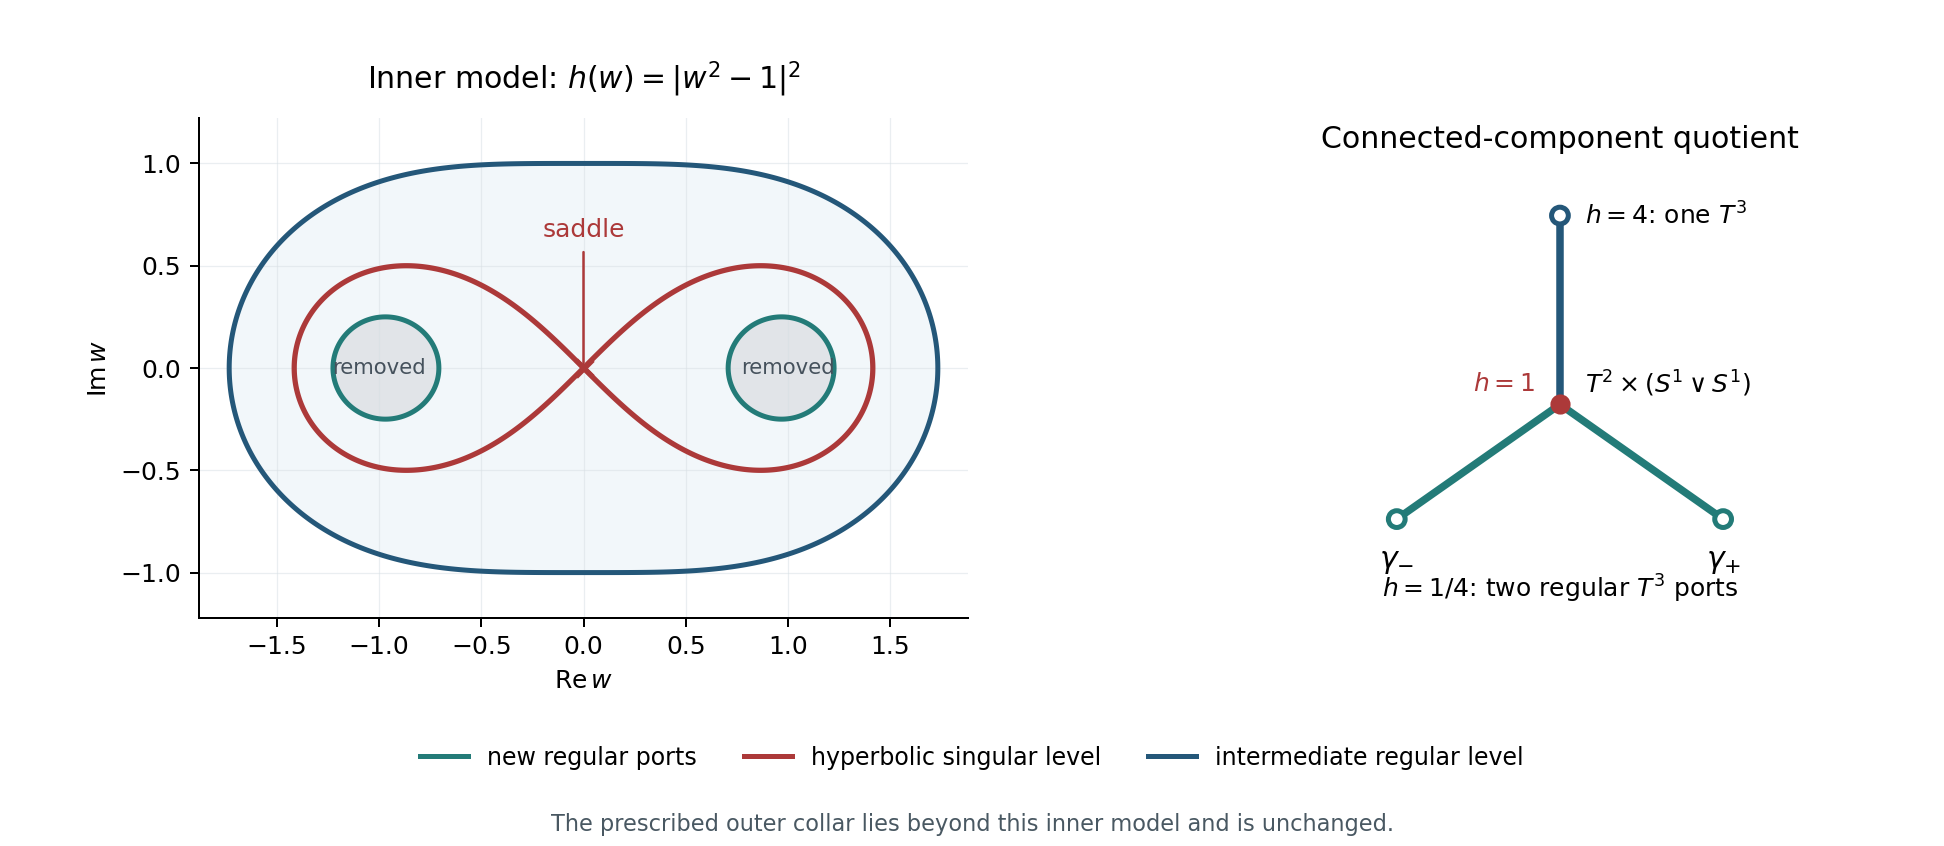
\includegraphics[width=\textwidth]{elliptic_pants_model.png}
\caption{Cutoff が恒等な内側での $|w^2-\nu|^2$ と connected-component quotient。
図は $\nu=1$、内側 cut $\eta=1/4$ の規格化であり、青線 $h=4$ は中間の正則 level である。
元の prescribed outer collar は図の範囲外にあり、相対構成では厳密に保持する。
灰色の二つの disk interiors を定義域から除く。表示していない shared $T^2$ との積を取ると、
赤い特異 level は $T^2\times(S^1\vee S^1)$ となる。}
\label{eb:inner-figure}
\end{figure}

\subsection{新しい ports の作用と cycle relation}

Outer circle を $\gamma_o$、二つの inner circles を $\gamma_+,\gamma_-$ とし、
いずれも normal disk の面積形式に関して反時計回りに向ける。
Inner circles のこの向きは、pants の boundary orientation と逆である。
Shared angles $\alpha_1,\alpha_2$ を固定して取れば
\begin{equation}\label{eb:cycle-relation}
 [\gamma_o]=[\gamma_+]+[\gamma_-]
 \quad\text{in }H_1(\text{pair of pants};\ZZ)
\end{equation}
となり、shared $T^2$ の cycle は付加されない。
$\gamma_\pm$ はそれぞれ primitive であり、元の filled cap では取り除いた actual symplectic disks を張る。

\begin{proposition}[Lobe actions の明示式]\label{eb:lobe-action}
$0<t<\nu^2$ における二つの sublevel disks は同じ面積
\begin{equation}\label{eb:lobe-integral}
 \mathcal A_\nu(t)
   =\frac1{4\pi}\int_{|u-\nu|\le\sqrt t}\frac{dA_u}{|u|}
\end{equation}
を持ち、
\begin{equation}\label{eb:lobe-bounds}
 \frac{t}{4(\nu+\sqrt t)}
 \le\mathcal A_\nu(t)
 \le\frac{t}{4(\nu-\sqrt t)}
\end{equation}
となる。
Saddle における各 lobe の面積と、上側 circle の action limit は
\begin{equation}\label{eb:saddle-actions}
 \mathcal A_\nu(\nu^2)=\frac\nu\pi,
 \qquad \mathcal A_o(\nu^2)=\frac{2\nu}{\pi}
     =\mathcal A_+(\nu^2)+\mathcal A_-(\nu^2).
\end{equation}
Outer port $p=g(I)$ と二つの inner ports $h_\nu=\eta$ では
\begin{equation}\label{eb:port-actions}
 \int_{\gamma_o}\lambda_0=g(I),\qquad
 \int_{\gamma_\pm}\lambda_0=\mathcal A_\nu(\eta)>0,
 \qquad
 \operatorname{Area}(\text{pants}_I)=g(I)-2\mathcal A_\nu(\eta).
\end{equation}
\end{proposition}

\begin{proof}
$w$-plane の Euclidean area を $dA_w$ とすると、normal symplectic form は
$dp\wedge d\theta=dA_w/\pi$ である。
$u=w^2$ は各 sublevel disk から $|u-\nu|\le\sqrt t$ への diffeomorphism で、
Jacobian は $4|u|$ だから式\eqref{eb:lobe-integral}を得る。
積分領域で $\nu-\sqrt t\le|u|\le\nu+\sqrt t$ を使うと式\eqref{eb:lobe-bounds}となる。
Critical lobe には式\eqref{eb:lemniscate}を直接用い、
\[
 \int_{-1/8}^{1/8}2\nu\cos(4\pi\theta)\,d\theta=\frac\nu\pi
\]
を得る。もう一方の lobe も同じであり、upper sublevel の面積はその和に連続して収束する。
各 regular circle での primitive period は、それが囲む normal disk の面積である。
Outer circle では $p=g(I)$ が一定なので period は $g(I)$。
Inner circles では式\eqref{eb:lobe-integral}となり、最後の式は Stokes の定理である。
\end{proof}

$\eta=\nu^2/4$ と取れば $\nu/24\le\mathcal A_\nu(\eta)\le\nu/8$ である。
Saddle における三つの action limits は厳密に加法的だが、
異なる高さにある三つの boundary actions の差には、式\eqref{eb:port-actions}の pants 面積が入る。
また $\mathcal A_\nu'(t)>0$ であり、saddle に近づく derivative の発散は通常の hyperbolic behavior である。
これは $h_\nu$ 自体の滑らかさの問題ではない。

\subsection{Primitive discrepancy の二つの ports への分配}

\begin{proposition}[Primitive の相対延長条件]\label{eb:primitive-split}
Outer collar に指定した primitive が
\begin{equation}\label{eb:outer-primitive}
 \lambda_{\rm old}
 =\lambda_0+c_1^T d\alpha_1+c_2^T d\alpha_2+c_o d\theta+dF
\end{equation}
と書けるとする。$c_1^T,c_2^T,c_o$ は connected parameter domain 上の定数である。
任意の定数 $c_+,c_-$ に対し、同じ $\omega$ の smooth primitive を pants 全体に延長し、
outer collar では $\lambda_{\rm old}$ と厳密に一致させ、inner meridian periods を
\begin{equation}\label{eb:inner-periods}
 \mathcal A_\nu(\eta)+c_+,\qquad \mathcal A_\nu(\eta)+c_-
\end{equation}
とするための必要十分条件は
\begin{equation}\label{eb:period-split}
 c_++c_-=c_o
\end{equation}
である。Shared periods は $I_j+c_j^T$ となる。
\end{proposition}

\begin{proof}
二つの中心 $\pm\sqrt\nu$ は除いた disks の内部にあるので、
\[
 \zeta_0=c_+\frac{d\arg(w-\sqrt\nu)}{2\pi}
            +c_-\frac{d\arg(w+\sqrt\nu)}{2\pi}
\]
は pants 全体で滑らかな closed one-form である。
その inner periods は $c_+,c_-$、outer period は $c_++c_-=c_o$ となる。
Outer annulus で $\zeta_0-c_o d\theta$ は period が零だから exact である。
これを $df$ と書き、その annulus に support を持ち outer collar で $1$ となる cutoff $\kappa$ により
\[
 \zeta=\zeta_0-d(\kappa f)
\]
とすれば、$\zeta=c_o d\theta$ が outer collar で厳密に成り立つ。
同じく $F$ を outer collar から cutoff を使って延長し、
\[
 \lambda_{\rm ext}
 =\lambda_0+c_1^T d\alpha_1+c_2^T d\alpha_2+\zeta+d\widetilde F
\]
と定めれば所要の primitive を得る。
逆に任意の延長の $\lambda_0$ との差は closed であり、
式\eqref{eb:cycle-relation}により式\eqref{eb:period-split}が必要となる。
また shared cycles は全 domain で同じ homology classes なので、shared periods も記載した通りである。
\end{proof}

式\eqref{eb:outer-primitive}は、outer collar の三つの marked periods が一致すれば、
残る closed difference が exact となることを明示している。
ここで $P$ が contractible なので、collar の $H^1$ は三つの torus cycles で尽くされる。
閉形式の periods は parameter に沿って局所一定であり、$c_\pm$ を自由な parameter-dependent functions に
置き換えてよいわけではない。

$\delta$ cap では元の primitive が filled disk 全体へ既に延びているので、
そのまま制限して $c_o=c_+=c_-=0$ とできる。
この場合、二つの inner periods は共に正の $\mathcal A_\nu(\eta)$ となる。

\begin{corollary}[Natural cap の discrepancy]\label{eb:natural-periods}
第\ref{kc:section}節の natural cap で $r=A-I_i^0$ と置く。
Transported flat angles を使えば、outer collar で $\theta_x=\alpha_1+\theta$ となり、
exact term を除いて
\[
 \lambda_{\rm old}=\lambda_{\rm cap}-r(d\alpha_1+d\theta)
\]
である。
従って元の primitive は pants 全体へ延長でき、二つの inner corrections は
\[
 c_++c_-=-r
\]
を満たす任意の定数に選べる。
Shared periods は $I_1-r,I_2$ であり、二つの inner meridian periods を同時に正にできる必要十分条件は
\begin{equation}\label{eb:both-positive}
 2\mathcal A_\nu(\eta)>r
\end{equation}
である。
\end{corollary}

\begin{proof}
Flat cap で $\alpha_1=\theta_u+\theta_v$、$\theta=\theta_w-\theta_u-\theta_v$ なので
$\theta_x=\theta_w=\alpha_1+\theta$ となる。
第\ref{kc:section}節の primitive difference は $r\,d\theta_x$ であり、
$SU(2)$ suspension と最後の inverse straightening を通して同じ boundary periods が保持される。
従って命題\ref{eb:primitive-split}で $c_1^T=-r,c_2^T=0,c_o=-r$ とすればよい。
二つの inner periods の和は $2\mathcal A_\nu(\eta)-r$ なので、両方が正なら式\eqref{eb:both-positive}が必要である。
逆にこの式が成り立てば $c_+=c_-=-r/2$ と取れば両方が正になる。
\end{proof}

式\eqref{eb:both-positive}が失敗しても regular $T^3$ port 自体への障害ではない。
Regular port の marked primitive period は負でもよい。
障害となるのは、その同じ oriented meridians を正面積の symplectic disks で埋め、
指定 primitive を disks 全体へ滑らかに延ばす条件を追加した場合である。
Pants への交換は discrepancy を二つの穴へ運ぶが、その総和を消さない。

\subsection{Hyperbolic fiber まで延びる周期的作用の格子}

新しい pants は shared $T^2$ を保つが、outer torus の第三の周期的作用まで保存するわけではない。
この差は、saddle に近づく normal period の発散で厳密に検出できる。

\begin{proposition}[延長可能な周期作用は shared lattice]\label{eb:periodic-lattice}
定理\ref{eb:pants}の product model で、外側 regular tori 上の cycle を
\[
 v=m_1e_1+m_2e_2+n\gamma_o\qquad(m_1,m_2,n\in\ZZ)
\]
とする。ここで $e_j$ は $\alpha_j$ の周期 $1$ orbit、$\gamma_o$ は positive normal circle である。
この cycle を生成する fibrewise Hamiltonian $S^1$ action の generator が、
whole hyperbolic singular fiber まで連続に延びる必要十分条件は $n=0$ である。
従って滑らかに延びる周期作用の格子は $\ZZ e_1\oplus\ZZ e_2$ である。
同じ結論は fibrewise symplectic $S^1$ actions にも成り立つ。
\end{proposition}

\begin{proof}
$t>\nu^2$ が十分近ければ、whole sublevel disk $\{h_\nu\le t\}$ は cutoff が $1$ の領域に入る。
$u=w^2$ は $|u-\nu|\le\sqrt t$ 上で、branch point を除き二重被覆である。
従って outer action とその derivative は
\begin{align}
 \mathcal A_o(t)
   &=\frac1{2\pi}\int_{|u-\nu|\le\sqrt t}\frac{dA_u}{|u|},
       \label{eb:outer-action-integral}\\
 T_o(t)=\mathcal A_o'(t)
   &=\frac1{4\pi}\int_0^{2\pi}
       \frac{d\phi}{|\nu+\sqrt t\,e^{i\phi}|}.
       \label{eb:outer-period}
\end{align}
面積の derivative $T_o(t)$ は、$h_\nu$ の Hamiltonian flow が normal circle を一周する時間である。
$\phi=\pi$ の近くで分母は
\[
 \sqrt{(\sqrt t-\nu)^2+2\nu\sqrt t\,(1+\cos\phi)}
\]
となる。従って $t\downarrow\nu^2$ で積分は logarithmically に発散し、$T_o(t)\to+\infty$ である。

Regular chamber 上では $(I_1,I_2,\mathcal A_o(h_\nu))$ が action coordinates になる。
Fibrewise symplectic vector field の $\iota_X\omega$ は closed であり、
Lagrangian fiber 上で零なので、局所的には base 上の closed one-form の pullback である。
従ってその係数は torus angles に依存しない。
周期 $1$ の flow の cycle が $v$ であることから、その Hamiltonian は局所定数を除いて
\[
 m_1I_1+m_2I_2+n\mathcal A_o(h_\nu)
\]
であり、generator は
\begin{equation}\label{eb:periodic-generator}
 X_v=m_1\partial_{\alpha_1}+m_2\partial_{\alpha_2}
               +nT_o(h_\nu)X_{h_\nu}
\end{equation}
となる。Integer coefficients は connected regular chamber 上で一定である。

Figure-eight の saddle 以外の点 $w_0$ を取り、外側 circles 上の点 $w_t\to w_0$ を選ぶ。
$X_{h_\nu}(w_t)\to X_{h_\nu}(w_0)\ne0$ である一方、$T_o(t)\to+\infty$ となる。
Shared directions と normal direction は product で独立なので、$n\ne0$ なら
式\eqref{eb:periodic-generator}はこの regular separatrix point の近くで非有界となり、連続に延びない。
$n=0$ なら shared rotations 自体が全 product 上で滑らかに定義されるので十分である。
\end{proof}

\begin{corollary}[二種類の caps に対する延長格子]\label{eb:marked-lattices}
元の upper torus の cycle を $v=m\gamma_U+\ell\Gamma_H+r\Gamma_J$ とする。
Natural cap の pants replacement を越えて延びる fibrewise periodic actions は
\[
 m=0,\qquad
 \Lambda_{\rm natural}=\operatorname{span}_{\ZZ}(\Gamma_H,\Gamma_J)
\]
である。一方、$\delta$ cap の pants replacement では
\[
 \ell+r=0,\qquad
 \Lambda_\delta=\operatorname{span}_{\ZZ}(\gamma_U,\Gamma_H-\Gamma_J)
\]
となる。
\end{corollary}

\begin{proof}
Natural product の shared cycles は $\Gamma_H,\Gamma_J$、normal cycle は $\gamma_U$ である。
$\delta$ product では shared cycles は $e_x,e_z$、normal cycle は $e_y=\delta$ であり、
第\ref{acp:section}節の関係から
\[
 v=(m+\ell)e_x+(\ell+r)e_y-r e_z
\]
となる。命題\ref{eb:periodic-lattice}を適用すればよい。
また $e_x=\gamma_U$、$e_z=\Gamma_H-\gamma_U-\Gamma_J$ なので、
shared lattice は記載した二つの generators でも表される。
\end{proof}

特に旧 $\Gamma_H$ と $\Gamma_J$ は、それぞれ $\delta$ の toric cap では周期作用として延びたが、
新しい $\delta$ pants の fibrewise $S^1$ action としては延びない。
両者の差 $\Gamma_H-\Gamma_J$ は延びる。
元の radial coordinate $p$ 自体は smooth function として残るが、
新しい $h_\nu$ と可換ではないので、その回転作用は新しい fibers を保たない。
Scalar labels の smooth extension、whole-fiber foliation の一致、周期的 action lattice の延長は、
ここでも別の条件である。

\subsection{Nodal trade との区別と残る接続}

Symington の nodal trade \cite[Lemma 6.3, Theorem 6.5]{symington} は、
node と boundary edge を結ぶ embedded eigenray、その途中の他の nodes の不存在、
vanishing/collapsing covectors の lattice-basis 条件を仮定する。
同じ underlying topological base 上で affine structure と stratification を変更する手術であり、
topological boundary 自体を消す定理ではない。
その action-angle product だけから、今回の generic elliptic face の消失は従わない。

本節の構成は、corank-one hyperbolic な pants への交換を明示し、
旧 outer collar の whole foliation と labels を保持しつつ、elliptic full germ を実際に変更する。
その代わりに二つの disk families を定義域から外し、新しい regular ports を記録した。
全体構成に進むには、それらの対向領域、whole-fiber identifications、primitive periods、
parameter 側面との整合、actual $X_\tau$ 内での coverage を別途構成する必要がある。

\section{Regular ports を接ぐ還元曲面の面積と相対 Chern 収支}
\label{rsb:section}

Elliptic cap の内部を pair of pants に置き換えると、元の outer collar を保持したまま、
二つの新しい regular ports を作れる。しかし、この二端を接いで自由境界を消すことは、
局所的な pants の構成とは別の問題である。本節では、同じ自由な Hamiltonian $T^2$ と
一つの moment level を保つ接続に必要な面積条件を示す。
結論は、実際に接続領域が存在すると仮定したときの必要条件であり、
以下の整数条件を満たすだけでその領域が構成できるとは主張しない。

固定した smooth sextic $X=X_\tau$ に対し
\[
 [\omega]=\mathfrak a\mathsf H,\qquad
 c_1(TX)=-\mathsf H,\qquad \mathfrak a>0
\]
を用いる。従って $[\omega]+\mathfrak a c_1(TX)=0$ である。
本節で比較に使う reference disks は smooth mapped disks で十分であり、
symplectic または embedded であることは、明記する cap disks 以外には要求しない。

\subsection{Boundary covector と shared orbit の輸送}

Lefschetz hyperplane theorem により $X$ は単連結であるから
\cite[Corollary 2.3.4]{achinger-lefschetz-gc}、任意の Lagrangian torus $L\subset X$ 上の loop は
$X$ 内で smooth mapped disk を bound する。第\ref{ml:section}節の量を一般化して
\begin{equation}\label{rsb:theta}
 \Theta_L(v)=\int_D\omega+\frac{\mathfrak a}{2}\mu(D),
 \qquad [\partial D]=v\in H_1(L;\ZZ)
\end{equation}
と置く。異なる disk の差に対して Maslov 指数は $2c_1$、面積は $[\omega]$ だけ変わるので、
この量は disk の選択によらない。また $\pi_1(L)=H_1(L;\ZZ)$ と disk の結合を使えば、
$\Theta_L$ は homomorphism となる。

以下、$X$ のある開集合に period-one Hamiltonian $T^2$ action があり、
その moment map を $\nu$、正則値を $\eta$ とする。
$E\subset\nu^{-1}(\eta)$ は compact connected $T^2$-invariant submanifold with boundary で、
action は $E$ 全体で free と仮定する。還元を
\[
 \pi:E\longrightarrow\Sigma=E/T^2
\]
と書く。$\Sigma$ は compact connected oriented surface で、
境界の逆像 $L_i=\pi^{-1}(\partial_i\Sigma)$ は Lagrangian $T^3$ である。
二つの固定した orbit generators を $\Gamma_1,\Gamma_2$ と書く。

各 $L_i$ に対する $\Theta_{L_i}$ の shared subgroup への制限は、
$E$ 内の orbit transport に関して同一の covector
\begin{equation}\label{rsb:shared-covector}
 \Theta_\Gamma:\ZZ^2\longrightarrow\RR
\end{equation}
となる。実際、二つの quotient points を path で結び、その上の orbit cylinder を取る。
Cylinder の一方向は $X_{\nu_a}$、他方向は $T\nu^{-1}(\eta)$ に属するので、
その symplectic area は零である。
Vertical isotropic plane $V=\langle X_{\nu_1},X_{\nu_2}\rangle$ は全域で framing を持つ。
Quotient の tangent line を path に沿って選ぶと、$V$ とその lift の和は cylinder 上の
Lagrangian boundary-data homotopy を与える。端では所定の $TL_i$ と一致させられる。
従って cylinder を使った比較は Maslov 指数も変えず、式\eqref{rsb:shared-covector}が従う。
これは shared moments の値が同じであることを用いる。
異なる moment levels を通る接続に、そのまま適用することはできない。

\subsection{Section に沿う Maslov 指数}

\begin{lemma}[自由な二つの作用を持つ還元曲面]\label{rsb:maslov-section}
$\partial\Sigma\ne\varnothing$ とする。Principal $T^2$ bundle $E\to\Sigma$ は
smooth section $s$ を持ち、任意の section について
\begin{equation}\label{rsb:section-data}
 \int_{s(\Sigma)}\omega=\operatorname{Area}(\Sigma)>0,
 \qquad
 \mu(s^*TX,TL_i|_{s(\partial_i\Sigma)})=2\chi(\Sigma)
\end{equation}
が成り立つ。
\end{lemma}

\begin{proof}
$H^2(\Sigma;\ZZ^2)=0$ より principal $T^2$ bundle は trivial である。
また $\omega|_E=\pi^*\omega_{\rm red}$ なので、section は symplectic であり、
その面積は還元面積に等しい。
$V$ は section の tangent plane と symplectically orthogonal なので、
section の rank-four symplectic normal bundle の Lagrangian subbundle となる。
その bundle は二つの Hamiltonian vector fields で framing を持つ。
Section の tangent plane と normal bundle を保つ compatible almost complex structure を選べば、
normal bundle は $V\oplus JV\simeq\CC^2$、その boundary real plane は $V\simeq\RR^2$ である。
さらに境界では $TL_i=ds(T\partial_i\Sigma)\oplus V$ であるため、bundle pair は
\[
 (s^*TX,TL|_{\partial\Sigma})
 \simeq (T\Sigma,T\partial\Sigma)\oplus(\CC^2,\RR^2)
\]
となる。Boundary tangent line の relative Chern number は Poincar\'e--Hopf により
$\chi(\Sigma)$、Maslov 指数はその二倍である。
従って式\eqref{rsb:section-data}を得る。
ここで singular fibers の内部に Lagrangian tangent line field を延ばしているのではない。
必要なのは regular boundary tori の tangent planes と、全 $E$ 上の free orbit framing である。
\end{proof}

\subsection{符号と相対 section defect を含む収支}

各 boundary torus $L_i$ 上に、positive-area Maslov-two cap disk $D_i$ と
その正向き子午線 $v_i=\partial D_i$ を指定し、$A_i=\int_{D_i}\omega>0$ と書く。
この reference disk は、候補の接続領域に含まれている必要はない。
子午線の quotient degree は $\pm1$ と仮定する。
Section の oriented boundary class は一意に
\begin{equation}\label{rsb:boundary-data}
 [s(\partial_i\Sigma)]=\sigma_i v_i+m_{i1}\Gamma_1+m_{i2}\Gamma_2,
 \quad \sigma_i\in\{1,-1\},\quad m_i\in\ZZ^2
\end{equation}
と書ける。$\sigma_i$ は $\Sigma$ の induced boundary orientation と
positive cap meridian の向きの比較であり、全てが $+1$ であるとは仮定しない。
定義
\begin{equation}\label{rsb:defect}
 e=\sum_i m_i\in\ZZ^2
\end{equation}
を、この指定に対する relative section defect と呼ぶ。

Section を変えると $m_i$ は $f:\Sigma\to T^2$ の boundary degrees だけ変わる。
その総和は零であるため $e$ は section によらない。
逆に $e=0$ なら、総和零の指定 boundary degrees を持つ $f$ を取り、
section を変えて全ての $m_i$ を零にできる。
従って $e=0$ は、指定した子午線の section representatives を boundary homotopy で選び直した後、
同時に一つの global section へ延ばせる条件である。
これは boundary marking に相対的な条件であり、
absolute bundle の triviality $H^2(\Sigma;\ZZ^2)=0$ とは区別する。

\begin{theorem}[還元接続領域の面積・Euler 収支]\label{rsb:budget}
上の仮定の下で
\begin{equation}\label{rsb:full-budget}
 \boxed{\quad
 \operatorname{Area}(\Sigma)+\mathfrak a\chi(\Sigma)
 =\sum_{i=1}^b\sigma_i(A_i+\mathfrak a)+\Theta_\Gamma(e).
 \quad}
\end{equation}
特に $e=0$ の場合は
\begin{equation}\label{rsb:untwisted-budget}
 \operatorname{Area}(\Sigma)
 =\sum_i\sigma_i A_i+\mathfrak a\left(\sum_i\sigma_i-\chi(\Sigma)\right)>0
\end{equation}
が必要である。
\end{theorem}

\begin{proof}
Section の各 boundary loop を、$L_i$ 内の zero-area chain も用いて
$\sigma_i v_i+m_i\cdot\Gamma$ と比較する。
Shared loops に reference mapped disks を取り、$s(\Sigma)$ から
$\sum_i\sigma_iD_i$ と shared reference disks を差し引けば、closed integral two-cycle $C$ を得る。
Maslov の sewing rule により
\[
 2\langle c_1(TX),C\rangle
 =2\chi(\Sigma)-2\sum_i\sigma_i-\sum_i\mu(D_i(m_i\cdot\Gamma)).
\]
面積の対応する差と合わせて
$\langle[\omega]+\mathfrak a c_1(TX),C\rangle=0$ を使うと、
\[
 \operatorname{Area}(\Sigma)+\mathfrak a\chi(\Sigma)
 =\sum_i\sigma_i\left(A_i+\frac{\mathfrak a}{2}\cdot2\right)
  +\sum_i\Theta_{L_i}(m_i\cdot\Gamma).
\]
Shared covector の transport invariance により最後の項は $\Theta_\Gamma(e)$ である。
Reference disks が embedded または symplectic であることは、この comparison に不要である。
\end{proof}

\subsection{Pants、annulus、handle の区別}

$e=0$ の場合の具体例は次の通りである。
\[
\begin{array}{c|c|c|c}
 \Sigma&\chi(\Sigma)&(\sigma_i)&\operatorname{Area}(\Sigma)\\\hline
 \text{disk}&1&(+) &A_1\\
 \text{pair of pants}&-1 &(+,-,-)&A_0-A_1-A_2\\
 \text{annulus}&0 &(+,-)&A_+-A_-\\
 \text{annulus}&0 &(+,+)&A_1+A_2+2\mathfrak a\\
 \Sigma_{g,1}&1-2g &(+)&A_1+2g\mathfrak a
\end{array}
\]
例えば cap 内の pants は outer boundary に正、二つの inner boundaries に負の向きを持つ。
その面積は $A_0-A_1-A_2$ であり、局所的な Stokes の計算と一致する。
これに対し、二つの inner ports を annulus で接いで閉じる場合、
annulus 側の境界は両方とも正向き子午線となる。
Relative section defect が零なら、その annulus は $A_1+A_2+2\mathfrak a$ の面積を必要とする。
Pants とこの annulus の和は once-punctured torus となり、全体の面積は $A_0+2\mathfrak a$ である。
同じ向きの二端を接ぐことと、向きが逆の二端を正則 cylinder で輸送することを、同一視してはいけない。

より一般に、$b$ 個の positive cap meridians を全て正向きの boundary とし、
defect が零なら
\begin{equation}\label{rsb:all-positive}
 \operatorname{Area}(\Sigma_{g,b})=\sum_i A_i+2\mathfrak a(g+b-1).
\end{equation}
これは genus や boundary gluing を入れる際の ambient area の必要量であり、存在定理ではない。

\begin{corollary}[Exact な近傍だけでは閉じない]\label{rsb:exact-obstruction}
式\eqref{rsb:all-positive}の接続領域と全 reference cap disks が同じ exact symplectic open set
$U\subset X$ に含まれ、$e=0$ とする。このとき $g+b=1$ が必要であり、
connected な置換は $g=0,b=1$ の disk の場合に限られる。
従って二つの inner ports を、その positive meridians と global section を保って
同じ exact な cap neighborhood 内で annulus により閉じることはできない。
\end{corollary}

\begin{proof}
全 boundary sections を指定 meridians と一致させる。
$\omega=d\lambda$ と Stokes により
$\operatorname{Area}(\Sigma)=\sum_i A_i$ である。
式\eqref{rsb:all-positive}との比較から $2\mathfrak a(g+b-1)=0$ を得る。
\end{proof}

\begin{corollary}[Section を持つ閉還元面の genus]\label{rsb:closed-section}
同じ free Hamiltonian $T^2$-level の還元が closed connected surface $\Sigma_g$ で、
principal bundle $E\to\Sigma_g$ が global section を持つと仮定する。このとき
\[
 \operatorname{Area}(\Sigma_g)=2\mathfrak a(g-1)>0,
 \qquad g\ge2.
\]
\end{corollary}

\begin{proof}
Section 上の complex tangent bundle は $T\Sigma_g\oplus\CC^2$ と同定できるため、
$\langle c_1(TX),s_*[\Sigma_g]\rangle=\chi(\Sigma_g)=2-2g$ である。
負の単調性と $s^*\omega=\omega_{\rm red}$ を使えば結論を得る。
\end{proof}

Closed surface の場合、principal $T^2$ bundle の section の存在は自動的ではない。
例えば第\ref{cf:sphere}節の $S^2$ reduction は nontrivial torus bundle を持つ。
従ってこの系から全ての compact spherical reductions を排除してはいけない。

\subsection{Natural caps の二端には twisting を許しても残る下界}

第\ref{kc:section}節の $k=2$ natural cap を、基準 slice $h=h_0,j=0$ で考える。
その old shared cycles は $\Gamma_H,\Gamma_J$ であり、第\ref{ml:section}節より
\begin{equation}\label{rsb:natural-covector}
 \Theta_\Gamma(e_H,e_J)=e_H(A_b+2\mathfrak a),
 \qquad 0<A_0<A_b<\mathfrak a.
\end{equation}
内側の二つの regular ports が positive Maslov-two disks $D_1,D_2$ を囲み、
その間の pants の面積が正なら $A_1+A_2<A_0$ である。

\begin{corollary}[Natural cap の two-port annulus の面積下界]\label{rsb:natural-bridge}
上の二端を、同じ global shared moments の同じ正則値の中で、
free $T^2$ reduction が annulus となる領域により接ぐと仮定する。
Annulus 側の二つの oriented boundary meridians は共に positive cap meridians とする。
任意の relative section defect $(e_H,e_J)$ を許しても
\begin{equation}\label{rsb:natural-bridge-area}
 \operatorname{Area}(\Sigma)
 =A_1+A_2+2\mathfrak a+e_H(A_b+2\mathfrak a),\qquad e_H\ge0.
\end{equation}
従って $\operatorname{Area}(\Sigma)\ge A_1+A_2+2\mathfrak a$ である。
元の wide contractible cap chart 内で、この接続を行うことはできない。
より一般には、annulus、二つの cap disks、shared orbit の reference disks を全て含む
同じ exact open set 内での接続は不可能である。
\end{corollary}

\begin{proof}
式\eqref{rsb:full-budget}に $\chi=0$, $\sigma_1=\sigma_2=1$ と
式\eqref{rsb:natural-covector}を代入する。
$e_H\le-1$ なら右辺は $A_1+A_2-A_b<0$ となり、正の還元面積に反する。
従って $e_H\ge0$ である。$e_J$ は基準 slice の収支に寄与しない。

Exact open set に全てが入ると仮定する。
その primitive の shared $\Gamma_H$-period は、reference cap chart で $A_b$ であり、
$\Gamma_J$-period は $0$ である。ここで、inner ports の当該 orbit loops を bound し、面積 $A_b,0$ を持つ
選定した reference disks も同じ exact set に入ることを仮定する。
Stokes により $\operatorname{Area}(\Sigma)=A_1+A_2+e_H A_b$ となる。
式\eqref{rsb:natural-bridge-area}と比較すると $e_H=-1$ を得るが、
その面積は $A_1+A_2-A_b<0$ となる。
特に元の wide contractible cap chart 内での接続は不可能である。
\end{proof}

最後の exact-neighborhood の結論で shared reference disks を含む仮定を落としてはいけない。
Natural cap の表示域は $u,v\ne0$ を満たすため、その小さい tube 自体は contractible とは限らない。
上の第一の面積下界はこの追加仮定を使わず、actual $X$ 内の候補 annulus に対する必要条件である。
また、shared action を別の subgroup に切り替える、moment values をずらす、
途中で action の自由性を失わせる、指定 boundary marking を変更する、という接続は、
この corollary の範囲外である。

\paragraph{使用した標準事項と証明の位置付け.}
Bundle pair の Maslov 指数、sewing と $2c_1$ の関係は
Cho--Shin \cite[\S\S2--4]{cho-shin-maslov} の定義と性質に従う。
Boundary tangent pair に対する $2\chi$ は relative Euler class の直接計算であり、
本節ではその計算と actual cap の境界データから上記の必要条件を導いた。
特定の接続領域の存在、全体の Hausdorff quotient、または全自由境界の消去は示していない。

% Research report for the parent; based on bundle v8.
\section{Delta pants の内側 ports と相対 twisting}
\label{dpb:section}

本節では第\ref{acp:section}節の $\delta$ cap と第\ref{eb:section}節の pants 交換を使う。
$\tau\ne0$、基準 outer torus の旧 parameters $h=h_0,j=0$ を固定し、
\[
 A_b=\operatorname{Area}(\Delta),\qquad
 \Delta_A=s(h-B),\qquad A_0=A_b-\Delta_A,
 \qquad 0<A_0<A_b<\mathfrak a
\]
とする。Distributed winding は $k\in\{1,2\}$ である。
以下の shared cycles は
\begin{equation}\label{dpb:shared}
 e_x=\gamma_U,\qquad
 e_z=\Gamma_H-\gamma_U-\Gamma_J
\end{equation}
であり、これらは新しい $\delta$-pants の全域で延びる。
Normal meridian は $e_y=\delta=\Gamma_H-\gamma_U$ である。

同じ shared moment level 上で、pants の二つの inner ports を $L_1,L_2$、
その内側の positive disks を $D_1,D_2$、正向き子午線を $v_i=\partial D_i$ とする。
Disk の interiors は現在の fibration domain から除かれているが、
actual $X_\tau$ と元の cap 内には存在する。
その面積を $A_i>0$ とすると
\begin{equation}\label{dpb:small}
 S:=A_1+A_2<\Delta_A.
\end{equation}
これは元の reduced cap disk の面積が $\Delta_A$ であり、残る pants が正面積を持つためである。

\subsection{Shared covector と annulus の数値条件}

\begin{proposition}[Delta shared covector]\label{dpb:covector}
各 inner torus 上で
\begin{equation}\label{dpb:theta}
 \Theta(e_x)=A_0+\mathfrak a(k-1),\qquad
 \Theta(e_z)=\Delta_A+\mathfrak a.
\end{equation}
Outer torus と同じ contractible disk neighborhood の reference frame では
\[
 \mathcal A_V(e_x)=A_0,\quad \mu_V(e_x)=2(k-1),\qquad
 \mathcal A_V(e_z)=\Delta_A,\quad \mu_V(e_z)=2.
\]
この reference neighborhood は fixed $\tau$ で initial scale を十分小さくして
cap と必要な reference disks 全体を含むように選ぶ。
\end{proposition}

\begin{proof}
Outer torus では式\eqref{dpb:shared}と命題\ref{ml:full-cycle}を使う。
$e_z$ の係数は $(p,\ell,r)=(-1,1,-1)$ なので、面積は $A_b-A_0=\Delta_A$、
Maslov 指数は $2(-(k-1)+k)=2$ である。
Inner ports への shared orbit transport は同じ fixed moment level の中で行う。
Product coordinates の shared isotropic plane は全域で framing を持ち、
normal line は critical orbit を避ける path に沿って補間できる。
Orbit cylinders の面積は零であり、Lagrangian boundary data は homotopy で接続するので、
shared areas と Maslov indices は変化しない。
これは内側 normal meridian の Maslov index が2であることと両立する。
\end{proof}

\begin{proposition}[Delta inner pair の annulus budget]\label{dpb:annulus-budget}
$L_1,L_2$ を、一つの free Hamiltonian $T^2$ の同じ regular moment level 内で接ぐ
compact connected invariant region があると仮定する。
その reduction は annulus $\Sigma$ で、両 boundary の向きは positive $v_i$ とする。
Shared generators は両 ports で式\eqref{dpb:shared}の marking と一致するとする。
Relative section defect を $(e_x^{\rm def},e_z^{\rm def})\in\mathbb Z^2$ と書くと
\begin{equation}\label{dpb:annulus-area}
 \operatorname{Area}(\Sigma)
 =S+2\mathfrak a
  +e_x^{\rm def}\bigl(A_0+\mathfrak a(k-1)\bigr)
  +e_z^{\rm def}\bigl(\Delta_A+\mathfrak a\bigr)>0.
\end{equation}
この数値条件は接続領域の存在を保証しない。
\end{proposition}

\begin{proof}
定理\ref{rsb:budget}で $\chi(\Sigma)=0$、$\sigma_1=\sigma_2=1$ とし、
式\eqref{dpb:theta}を代入する。
\end{proof}

\subsection{元の annular tube 内では twisting も genus も救わない}

元の actual annular tube $\mathcal T$ には、base circle の integral closed one-form
$\beta$ があり、cap 上の homology marking に対して
\begin{equation}\label{dpb:beta}
 \int_{e_x}\beta=1,\qquad \int_{e_z}\beta=0,
 \qquad \int_{v_i}\beta=0
\end{equation}
を満たす。Upper straightening の Hamiltonian isotopy を戻した後も、この period statement は不変である。
$\mathcal T$ は exact で、元の primitive の $e_z$ period は $\Delta_A$ である。

\begin{theorem}[Delta pair の tube 内接続障害]\label{dpb:tube}
命題\ref{dpb:annulus-budget}の接続領域全体が同じ actual annular tube $\mathcal T$ に
含まれることはない。この結論は任意の relative section defect を許す。
さらに reduction を任意の genus $g\ge0$ の二境界曲面 $\Sigma_{g,2}$ に変更しても不可能である。
Action は境界近傍で prescribed shared action と一致し、全接続領域で free であればよく、
内部全体で同じ explicit toric coordinate formula を保つ必要はない。
\end{theorem}

\begin{proof}
Principal $T^2$ bundle は boundary を持つ surface 上なので section $s$ を持つ。
Section の boundary marking を
\[
 [s(\partial_i\Sigma)]=v_i+m_{ix}e_x+m_{iz}e_z,
 \qquad e^{\rm def}=\sum_i m_i
\]
と書く。$d\beta=0$ と Stokes を section 上で使うと
\[
 0=\int_{s(\partial\Sigma)}\beta=e_x^{\rm def}.
\]
Tube の primitive を $\lambda$ とすると、shared orbit cylinders の area は零なので、
全境界で $e_z$ period は $\Delta_A$ と一致する。
Positive disks $D_i$ も tube 内にあるため、$\int_{v_i}\lambda=A_i$ である。
従って
\begin{equation}\label{dpb:tube-stokes}
 \operatorname{Area}(\Sigma)=S+e_z^{\rm def}\Delta_A.
\end{equation}
一方、面積・Maslov budget は $\chi(\Sigma_{g,2})=-2g$ より
\[
 \operatorname{Area}(\Sigma)
 =S+2\mathfrak a(g+1)
   +e_z^{\rm def}(\Delta_A+\mathfrak a).
\]
二式の比較から
\[
 e_z^{\rm def}=-2(g+1),\qquad
 \operatorname{Area}(\Sigma)=S-2(g+1)\Delta_A<0
\]
を得て矛盾する。最後の不等式には式\eqref{dpb:small}を使った。
\end{proof}

同じ議論は $b\ge1$ 個の positive normal disk ports に対しても成立する。
総面積を $S$ とすると、同じ shared level と同じ tube の仮定の下で
\begin{equation}\label{dpb:general-tube}
 e_x^{\rm def}=0,\qquad
 e_z^{\rm def}=\chi(\Sigma)-b=-2(g+b-1),\qquad
 \operatorname{Area}(\Sigma)=S-2(g+b-1)\Delta_A.
\end{equation}
従って、それらの disks が一つの元 cap 内の互いに素な subdisks で $S<\Delta_A$ なら、
$g+b\ge2$ の connected closure は不可能である。
$g=0,b=1$ ではこの障害はなく、元の disk filling はまさにこの場合である。
この主張は shared free $T^2$ と同じ moment level を維持する closure に関するものであり、
その自由性を失う singular stratum、shared subgroup の変更、異なる moment levels の接続は対象外である。

\subsection{Wide exact chart の算術は別になる}

Annular tube の外へ出ると、式\eqref{dpb:beta}の closed one-form が接続領域全体に
延びるとは限らない。従って $e_x^{\rm def}=0$ を ambient 全体で課してはいけない。
この点で natural inner pair の $2\mathfrak a$ 下界とは異なる。

\begin{proposition}[Exact chart 内の必要な defect]\label{dpb:wide}
命題\ref{dpb:annulus-budget}の候補接続、二つの positive disks、
および $e_x,e_z$ の上記 reference disks が同じ exact open set $V$ に含まれると仮定する。
このとき
\begin{align}
 e_z^{\rm def}&=-2-(k-1)e_x^{\rm def},\label{dpb:exact-defect}\\
 \operatorname{Area}(\Sigma)
 &=S-2\Delta_A
   +e_x^{\rm def}\bigl(A_0-(k-1)\Delta_A\bigr)>0.\label{dpb:exact-area}
\end{align}
特に $C_k:=A_0-(k-1)\Delta_A=A_b-k\Delta_A>0$ なら
\[
 e_x^{\rm def}>\frac{2\Delta_A-S}{C_k}>0.
\]
これは actual 接続の存在定理ではなく、必要な section defect の算術である。
\end{proposition}

\begin{proof}
Reference disks が同じ exact set に入るという仮定により、その primitive の periods は
$A_0,\Delta_A,A_1,A_2$ である。従って Stokes は
\[
 \operatorname{Area}(\Sigma)=S+e_x^{\rm def}A_0+e_z^{\rm def}\Delta_A
\]
を与える。式\eqref{dpb:annulus-area}との比較が第一式であり、代入が第二式である。
\end{proof}

例えば $\Delta_A<A_b/(k+2)$ となるよう scale を小さくすると、
\[
 e_x^{\rm def}=1,\qquad e_z^{\rm def}=-(k+1)
\]
は数値条件を通過し、
\[
 \operatorname{Area}(\Sigma)=S+A_b-(k+2)\Delta_A>0
\]
となる。$k=1$ では defect $(1,-2)$、$k=2$ では $(1,-3)$ である。
この数値例は、$\delta$ 型に対する $2\mathfrak a$ の追加面積の下界を、
同じ面積・Maslov 収支だけからは導けないことを示す。
しかし、それらの integers と area を持つ embedded coisotropic connection はここでは構成していない。
実際の候補は、base angle の全域延長を失うほど annular tube の外へ出る必要がある。

\paragraph{今後の構成上の結論.}
48 ports のうち $\delta$ 型の一組を、同じ tube 内の free shared-level surface で閉じる方式は
任意の twisting と genus を含めて除外された。
一方、ambient exact chart への進出には明示的な positive defect 候補があり、
その actual realization は別の幾何学的問題として残る。
新しい shared subgroup や singular orbit を使う接続方式も、この定理の対象外である。

\section{閉曲線の正 normal shell と一価頂点のない分岐 graph}
\label{ncb:section}

本節では、閉じた平面切断曲線の全体を使う別の actual block を構成する。
その曲線方向の基底には一価の頂点がなく、特異 fibers は corank-one hyperbolic 型のみである。
Normal moment の有限 window による側面は残る。
前節までの24個の annular collars を固定する相対定理でも、48本の新 regular ports を
接続したという主張でもない。閉曲線の topology と非自明な normal bundle を同時に使う
構成を、今後の接続に使える独立の出発点として与える。

\subsection{極大・極小を持たない circle-valued Morse map}

次の曲面論の事実自体は既知である。
例えば de Rezende--Ledesma--Manzoli Neto--Vago の
\cite[Theorem 5.5, Lemma 5.7]{circle-morse-ncb}を参照されたい。
本稿では必要な genus と whole fibers を明示するため、pants の接着から構成する。

\begin{lemma}[一価頂点のない Reeb graph]\label{ncb:circle-morse}
$C$ を genus $g\ge2$ の closed connected oriented smooth surface とする。
Critical values が互いに異なる smooth map $f:C\to\RR/\ZZ$ を、
critical points がちょうど $2g-2$ 個で全て index one となるよう選べる。
その connected-level quotient $q:C\to\Gamma$ は finite connected Hausdorff graph であり、
\begin{equation}\label{ncb:graph-counts}
 \#V(\Gamma)=2g-2,\qquad
 \#E(\Gamma)=3g-3,\qquad b_1(\Gamma)=g.
\end{equation}
全 vertices は三価で、regular fibers は circles、vertex fibers は figure-eights である。
\end{lemma}

\begin{proof}
一つの incoming circle と二つの outgoing circles を持つ elementary pair of pants に、
唯一の critical point が index one である height function を入れる。
局所式 $x^2-y^2$ に regular collars を付加すればよい。
二つの incoming circles を一つに merge する逆向きの pants と、二本の中間 cuffs で接ぐ。
Boundary collars の height coordinates を一致させ、induced boundary orientations に関して
逆向きに接着することで、genus one、boundary 二つの oriented cobordism $B$ を得る。
Height は両端 collar で product coordinate となり、内部には split と merge の二つの saddles だけがある。

$n=g-1$ 個の $B_j$ を取り、height の値域を順に
$[j/n,(j+1)/n]$ とする（添字 $j=0,\ldots,n-1$）。
Outgoing circle と次の incoming circle を、height の product collars を保って接ぎ、
最後も最初へ巡回的に接ぐ。
値域の両端を modulo $1$ で同一視すると、滑らかな circle-valued map を得る。
各 $B_j$ の二つの critical values は、その区間の内部で全て異なるように選ぶ。
Seam の近くは product なので新しい critical points は生じない。
得られた surface は closed、connected、oriented であり、
\[
 \chi=\sum_{j=0}^{n-1}\chi(B_j)=-2n=2-2g.
\]
従って genus $g$ の $C$ へ orientation-preserving diffeomorphism で移せる。

各 $B_j$ の quotient は、二つの trivalent vertices を二本の parallel edges で結び、
それぞれに incoming と outgoing の cuff edge を持つ graph である。
巡回接着後、vertices は $2n$ 個、二本ずつの中間 edges が $2n$ 本、
隣接 $B_j$ を結ぶ edges が $n$ 本なので、$E=3n$ である。
Connected graph の $b_1=E-V+1$ より $b_1=n+1=g$ を得る。
この有限 graph への quotient は、pants と regular cylinders の connected-level quotients を
有限個接いだものなので Hausdorff である。Singular level は各 pants の figure-eight である。
\end{proof}

\begin{lemma}[可縮な regular level はない]\label{ncb:essential-circles}
Closed surface 上の circle-valued Morse map が extrema を持たなければ、
その regular level の各 circle component は surface 内で非可縮である。
\end{lemma}

\begin{proof}
可縮な embedded circle は disk $D$ を bound する。
$f|_D$ は $D$ の単連結性から実数値関数 $F$ へ lift でき、$F|_{\partial D}$ は定数である。
$F$ が非定数なら、境界値との大小に応じて interior maximum または minimum を持つ。
これは $f$ の extrema となる。$F$ が定数なら open disk 上に critical points があり、Morse 条件に反する。
\end{proof}

特に、閉曲線 $C^*$ の24個の削除円板の小さい境界 circles を、
この $f$ の regular level components として同時に保持することはできない。
この補題は base curve の circles に関する主張であり、
ambient 六次元多様体内の新しい regular ports の一般的接続を排除するものではない。

\subsection{平面切断曲線の global normal model}

以後 $X_d\subset\PP^4$ を smooth hypersurface、$d\ge6$、
$\omega$ を所定の K\"ahler form、$[\omega]=\mathfrak a\mathsf H$, $\mathfrak a>0$ とする。
二つの generic hyperplanes による切断を $C$ とすれば、$C$ は smooth plane curve of degree $d$ であり、
\begin{equation}\label{ncb:curve-data}
 g(C)=\frac{(d-1)(d-2)}2,\qquad
 \int_C\omega_C=d\mathfrak a,\qquad
 N_{C/X_d}\simeq\mathcal O_C(1)\oplus\mathcal O_C(1),
 \quad\omega_C=\omega|_C.
\end{equation}
Smoothness は generic hyperplane sections、normal bundle は二つの transverse equations の
conormal sequence から従う。Genus は $K_C\simeq\mathcal O_C(d-3)$ から得られる。
六次の既存 pencil では、命題\ref{ad:fixed-curve}の固定曲線 $C^*$ をそのまま使える。

Symplectic normal bundle を compatible complex structure と metric で complex rank two bundle と見て、
上の二つの line summands に対応する symplectically orthogonal splitting $L_1\oplus L_2$ を選ぶ。
第一の complex line とその Hermitian complement を取る方法でも、
第二の quotient line が $\mathcal O_C(1)$ と同型なので実現できる。
元の二つの非直交な complex normal lines を同時に固定することは要求しない。

角の周期は $1$、fiberwise actions は $p_j=\pi|z_j|^2$ とする。
Unit circle bundle $P(L_j)$ の connection $\alpha_j$ は
$\alpha_j(\partial_{\theta_j})=1$ と規格化し、
\begin{equation}\label{ncb:connections}
 d\alpha_j=\pi^*\kappa_j,
 \qquad [\kappa_j]=-c_1(L_j),
 \qquad \kappa_1=\kappa_2=-\frac{\omega_C}{\mathfrak a}
\end{equation}
となるよう選ぶ。最後の curvature form の積分は $-d$ で、所要の class と一致する。
任意の connection の curvature との差は exact なので、base one-form を加えてこの選択ができる。

Normal bundle の zero section の近傍に
\begin{equation}\label{ncb:omega}
 \begin{split}
 \Omega_N
 &=\pi^*\omega_C+\sum_{j=1}^2 d(p_j\alpha_j)\\
 &=\left(1-\frac{p_1+p_2}{\mathfrak a}\right)\pi^*\omega_C
       +dp_1\wedge\alpha_1+dp_2\wedge\alpha_2
 \end{split}
\end{equation}
を入れる。$p_j\alpha_j$ は $z_j=0$ へも滑らかに延びる。
Connection による horizontal--vertical splitting から、$p_1+p_2<\mathfrak a$ で symplectic であり、
zero section 上では所定の tangent form と normal fiber form に一致する。

\begin{lemma}[閉曲線全体に沿う actual normal embedding]\label{ncb:embedding}
ある $\varepsilon>0$ に対し、$p_1+p_2<\varepsilon$ の normal disk bundle から
$(X_d,\omega)$ への symplectic embedding $\Psi$ があり、zero section 上で $C$ への恒等写像となる。
その normal first jet は、選んだ symplectic normal bundle の同定と一致させられる。
$\varepsilon<\mathfrak a$ としてよい。
\end{lemma}

\begin{proof}
Zero section とその normal first jet を指定して smooth tubular embedding $F$ を取る。
$F^*\omega$ と $\Omega_N$ は zero section 上で full bilinear forms として一致する。
Normal radial homotopy による difference の primitive は $O(|z|^2)$ であり、
十分小さい disk bundle 上では両形式の直線補間が symplectic である。
Relative Moser field は zero section と normal first jet を固定する。
Compact な $C$ 全体に対して共通の radius を選び、その time-one map と $F$ を合成する。
これは symplectic neighborhood theorem の直接の relative Moser 証明である
\cite[Section 7.3, Theorem 7.4]{cds-local}。
所定の K\"ahler form 自体を変更するのではなく、模型からその form への symplectic embedding を作っている。
\end{proof}

\subsection{全曲線上の actual hyperbolic torus block}

\begin{theorem}[一般次数に対する一価頂点のない曲線方向の block]\label{ncb:actual-block}
式\eqref{ncb:curve-data}の $C\subset X_d$ に対し、十分小さい compact rectangle
\[
 P=[p_1^-,p_1^+]\times[p_2^-,p_2^+],
 \qquad 0<p_j^-<p_j^+,\qquad p_1^++p_2^+<\varepsilon
\]
を取る。Normal bundle 内の shell
\[
 \mathcal A_P=\{(z_1,z_2)\in L_1\oplus L_2:(p_1,p_2)\in P\}
\]
の actual image $\Psi(\mathcal A_P)\subset X_d$ 上に、connected Lagrangian fibers を持つ map
\begin{equation}\label{ncb:fibration}
 \Pi:\Psi(\mathcal A_P)\longrightarrow P\times\Gamma
\end{equation}
がある。$\Gamma$ は補題\ref{ncb:circle-morse}の一価頂点のない graph であり、
\begin{equation}\label{ncb:d-counts}
 \#V=d(d-3),\qquad
 \#E=\frac{3d(d-3)}2,\qquad
 b_1(\Gamma)=\frac{(d-1)(d-2)}2.
\end{equation}
Regular fibers は $T^3$、vertex fibers は $T^2\times(S^1\vee S^1)$ である。
各 vertex 上には $P$ で parameterize された nondegenerate rank-two hyperbolic orbit の族があり、
elliptic fibers は存在しない。Base は Hausdorff であり、曲線方向に free boundary はない。
一方 $\partial P\times\Gamma$ に沿う normal-action faces は残る。
\end{theorem}

\begin{proof}
模型上で
\[
 \Pi_N(z_1,z_2)=\bigl(p_1,p_2,q(\pi(z_1,z_2))\bigr)
\]
と定め、$\Psi$ で運ぶ。
Normal rotations は $\iota_{\partial_{\theta_j}}\Omega_N=-dp_j$ を満たす free Hamiltonian $T^2$ action である。
Circle-valued $f$ の各 local real lift $F$ に対し、$F\circ\pi$ は rotations に invariant なので、
$p_1,p_2,F\circ\pi$ は互いに Poisson commute する。
Regular point ではこれらの differentials は独立である。

Fixed $p=(p_1,p_2)$ の reduction は $C$ であり、その symplectic form は
\begin{equation}\label{ncb:reduction}
 \omega_p=\left(1-\frac{p_1+p_2}{\mathfrak a}\right)\omega_C.
\end{equation}
Regular circle $\gamma=q^{-1}(b)$ の inverse image 上では $dp_j=0$ である。
Base へ射影した tangent space は一次元なので、$\omega_C$ も curvature terms もそこで零になる。
従って inverse image は三次元 Lagrangian である。
Principal $T^2$ bundle の circle 上の制限は $H^2(S^1;\ZZ^2)=0$ により trivial であり、fiber は $T^3$ となる。

Critical point では $F$ の reduced Hessian が index one であり、$p_j$ の二つの free orbit directions と合わせて
nondegenerate corank-one hyperbolic 型になる。
Vertex の whole level component は figure-eight である。
その上でも $H^2(S^1\vee S^1;\ZZ^2)=0$ なので、principal bundle の制限は trivial であり、
whole singular fiber は $T^2\times(S^1\vee S^1)$ である。
この議論に $L_j$ の $C$ 全体での triviality は不要である。

各 fiber は connected で、compact source から compact Hausdorff space $P\times\Gamma$ への continuous surjection なので
表示は connected-fiber quotient である。
Formula \eqref{ncb:d-counts} は式\eqref{ncb:graph-counts}と genus formula の代入から従う。
Normal moments が正のため axes は domain に含まれず、$f$ に extrema がないため elliptic fibers はない。
\end{proof}

六次では、$g=10$、$\#V=18$、$\#E=27$、$b_1=10$ である。
この18は新しい shell の hyperbolic families の数であり、従来の24 caps からの families とは別の構成である。
両者を自動的に加算して一つの actual assembly の特異 fibers の数としてはならない。

\begin{figure}[htbp]
\centering
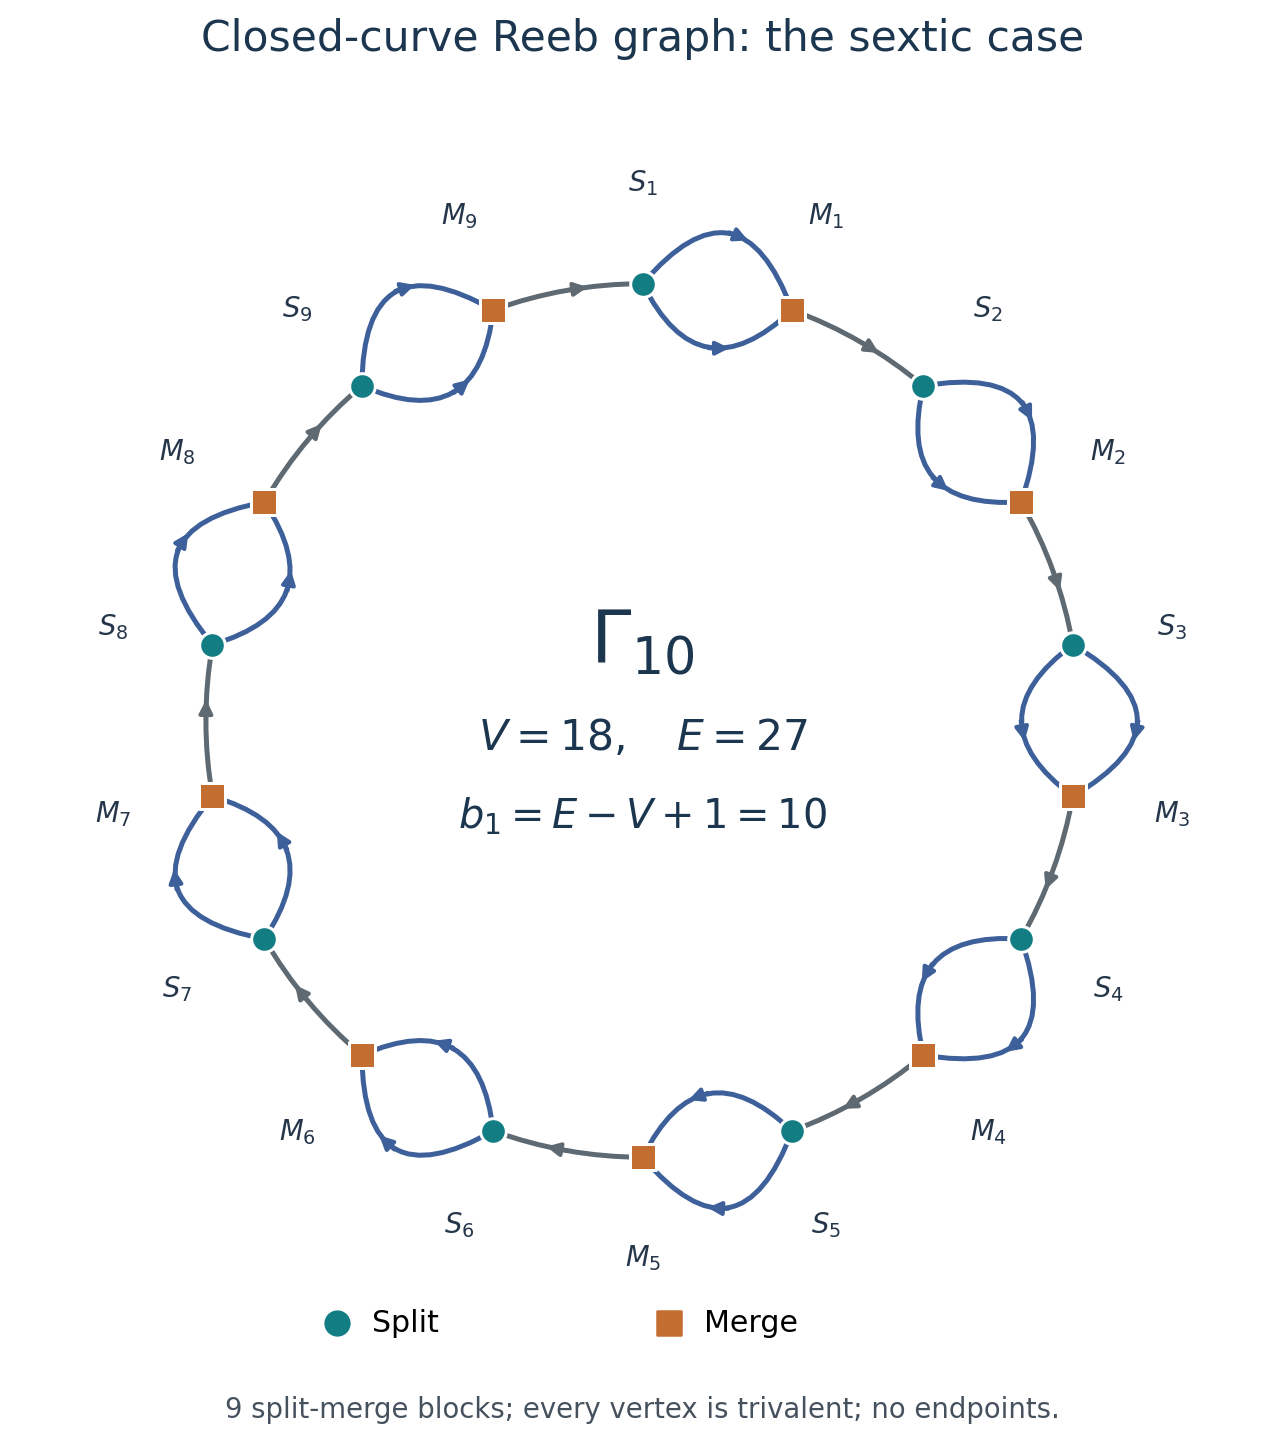
\includegraphics[width=0.83\textwidth]{closed_curve_graph.png}
\caption{六次の閉曲線に対する circle-valued Morse map の Reeb graph。
9個の split--merge cobordisms を巡回接着し、18頂点、27辺、$b_1=10$ を得る。
全頂点は三価である。Actual block の三次元基底は、この graph と二つの normal actions の
rectangle $P$ との積であり、$\partial P$ の側面は図示していない。}
\label{ncb:graph-figure}
\end{figure}

\paragraph{接続への意味と限界.}
この構成では、閉曲線の一周方向を circle-valued map にすることで、
曲線方向の extrema を最初から作らない。
ただし domain は zero section と二つの normal axes を含まず、normal moments の上下 faces も未接続である。
旧 curve block の transverse focus foliation と、ここで使う二つの normal rotations は異なる選択である。
24個の既定 annular germs、primitive constants、new pants ports との一致はこの定理の結論に含めない。
特に補題\ref{ncb:essential-circles}により、旧 puncture の contractible base cuffs をこの $f$ の
regular levels のまま保持することはできない。
既存48 ports との接続には、実際の overlap、period lattice と boundary coorientation の比較が必要である。
また二つの normal circles はこの shell には存在するが、系\ref{gc:hypersurface}により
全 $X_d$ の非自明な symplectic circle action として延長することはできない。

\subsection{Section を持たない閉還元面の Euler 補正}

前節の構成では、closed reduced surface は $C$ であるが、principal $T^2$ bundle の
Chern vector は $(d,d)$ であり section は存在しない。
従って系\ref{rsb:closed-section}を無条件には適用できない。
ここで必要な一般式を示す。

$(X,\omega)$ を simply connected symplectic six-manifold とし、
\[
 [\omega]+\nu c_1(TX)=0,\qquad\nu>0
\]
と仮定する。Shared orbit の boundary covector は、式\eqref{rsb:theta}で $\mathfrak a$ を $\nu$ に置換し、
\[
 \Theta_L(v)=\operatorname{Area}(D)+\frac\nu2\mu(D)
\]
と定める。前節と同じ comparison により well-defined であり、同じ free Hamiltonian $T^2$ の
同じ moment level 上で shared restriction $\Theta_\Gamma$ は一定である。

\begin{proposition}[閉還元面の面積・Euler class 収支]\label{ncb:closed-budget}
一つの regular moment level 内の compact free $T^2$-invariant submanifold $E$ の reduction を
closed connected oriented surface $\Sigma$ とする。
固定 generators に関する principal bundle の Chern vector を
\[
 c=(c_1,c_2)\in\ZZ^2,\qquad
 c_j=-\int_\Sigma\kappa_j
\]
とする。ここで $\alpha_j(\Gamma_k)=\delta_{jk}$、$d\alpha_j=\pi^*\kappa_j$ であり、
unit circle bundle of a complex line では $c_j$ はその line の degree である。
このとき
\begin{equation}\label{ncb:closed-budget-equation}
 \boxed{\quad
 \operatorname{Area}(\Sigma)+\nu\chi(\Sigma)+\Theta_\Gamma(c)=0.
 \quad}
\end{equation}
\end{proposition}

\begin{proof}
Small closed disk $D\subset\Sigma$ を取り、$\Sigma_0=\Sigma\setminus\operatorname{int}D$ とする。
両者の上に sections $s_D,s_0$ がある。
$v=\partial s_D(D)$ は正向きの base disk boundary を射影し、
area $A_D=\operatorname{Area}(D)>0$、Maslov index $2$ を持つ。
後者は補題\ref{rsb:maslov-section}の free orbit framing の証明を disk に適用して得られる。
Boundary torus 上で
\[
 [s_0(\partial\Sigma_0)]=-[v]+m_1\Gamma_1+m_2\Gamma_2
\]
と書く。$\alpha_j$ はこの boundary torus 上では closed であり、Stokes より
\[
 m_j
 =\int_{s_0(\partial\Sigma_0)}\alpha_j+\int_v\alpha_j
 =\int_{\Sigma_0}\kappa_j+\int_D\kappa_j
 =-c_j.
\]
従って式\eqref{rsb:full-budget}の $\nu$ 版を $\Sigma_0$ に適用すると
\[
 \operatorname{Area}(\Sigma_0)+\nu\chi(\Sigma_0)
 =-(A_D+\nu)-\Theta_\Gamma(c).
\]
$\chi(\Sigma_0)=\chi(\Sigma)-1$ と面積の加法性から結論を得る。
\end{proof}

\begin{corollary}[Normal shell の全次数の収支]\label{ncb:normal-budget}
定理\ref{ncb:actual-block}において $\nu=\mathfrak a/(d-5)$ と置く。
Positive normal rotations の reference disks は面積 $p_j$、Maslov index $2$ を持つので
\begin{equation}\label{ncb:normal-theta}
 \Theta_\Gamma(e_1,e_2)=e_1(p_1+\nu)+e_2(p_2+\nu).
\end{equation}
Reduction の area、Euler characteristic、Chern vector は
\begin{equation}\label{ncb:normal-numbers}
 \operatorname{Area}(C_p)=d(\mathfrak a-p_1-p_2),\qquad
 \chi(C)=d(3-d),\qquad c=(d,d).
\end{equation}
これらは式\eqref{ncb:closed-budget-equation}を満たす。
\end{corollary}

\begin{proof}
Reference disk は base point と他方の normal coordinate を固定し、$z_j$ の半径を零まで縮める
fiber disk である。Area は $p_j$、boundary tangent の一回転から Maslov index は $2$ である。
他の tangent directions はこの disk 上で framing されている。
Area formula は式\eqref{ncb:reduction}の積分、Euler characteristic は genus formula、
Chern vector は $\deg L_j=d$ から得られる。
全てを代入すると
\[
 \begin{split}
 &d(\mathfrak a-p_1-p_2)+\nu d(3-d)
       +d(p_1+p_2+2\nu)\\
 &\hspace{20mm}=d\mathfrak a+\nu d(5-d)=0.
 \end{split}
\]
従って、nontrivial normal bundle の Euler correction を含めると負の単調性と厳密に整合する。
\end{proof}

六次では reduction の面積は $6(\mathfrak a-p_1-p_2)$ であり、
section を持つ genus $10$ reduction の式 $18\mathfrak a$ とは異なる。
その差を担うのが $\Theta_\Gamma(6,6)=6(p_1+p_2+2\mathfrak a)$ である。
この補正は arbitrary gluing の存在を与えるものではないが、
閉曲線近傍に実際に存在する reduction を誤って除外しないために必要である。


\subsection{Zero section の coherent focus 充填への制約}

% Short application of existing lc:framing:hessian / lc:framing:chern.
% No new obstruction principle is claimed.
\paragraph{Zero section を全て同じ focus subsystem で埋めることへの制約.}
定理\ref{ncb:actual-block}の positive normal shell は zero section と normal axes を含まない。
これらを追加するとき、既存の tensor-line 障害
（補題\ref{lc:framing:hessian}、命題\ref{lc:framing:chern}）は次の形になる。

\begin{corollary}[Closed normal curve に沿う coherent focus の障害]
\label{ncb:closed-focus-obstruction}
$L_1\oplus L_2=N_{C/X_d}$、$L_j\simeq\mathcal O_C(1)$ とし、
normal circle を $H=p_1-p_2$ に固定する。
Zero section $C$ に沿う smooth real transverse integral $Q$ があり、
$Q|_C=0$、$\{H,Q\}=0$、かつ $H$ と $Q$ の normal quadratic pair が
$C$ の全点で nondegenerate focus--focus 型となることはない。
同じ結論は、global $Q$ の代わりに local generators $Q_a$ を使い、その normal quadratic parts が
\[
 [Q_a]=a_{ab}[Q_b]\pmod{\mathbb R H},\qquad a_{ab}\in\mathbb R^\times
\]
と変換する coherent transverse subsystem にも成り立つ。
\end{corollary}

\begin{proof}
$H$ は normal fibers に weights $(+1,-1)$ で作用する。
$Q|_C=0$ と invariance により $dQ|_C=0$ であり、normal Hessian は内在的に定まる。
$r_j=|z_j|^2/2$ と書き、$H$ の倍と正の period normalization を除けば
\[
 Q_2=t(r_1+r_2)+\operatorname{Re}(b z_1z_2)
\]
となる。Invariant quadratic monomials は $|z_1|^2,|z_2|^2,z_1z_2,\bar z_1\bar z_2$ だけである。
補題\ref{lc:framing:hessian}により focus 条件は $|b|^2>t^2$、特に $b\ne0$ を必要とする。
しかし $b$ は
\[
 (L_1\otimes L_2)^*\quad\text{の切断であり}\quad
 \deg((L_1\otimes L_2)^*)=-2d\ne0
\]
なので nowhere-zero section にはなれない。
Local real-generator transitions の場合も命題\ref{lc:framing:chern}により
$2c_1(L_1\otimes L_2)=0$ が必要であり、$H^2(C;\mathbb Z)\simeq\mathbb Z$ では不可能である。
\end{proof}

Smooth coefficient $b$ が zero section に transverse なら、その零点の局所指数は $\pm1$ であり、
符号付き総和は $-2d$ である。従って零点数は少なくとも $2d$ であるが、
一般にはちょうど $2d$ とは限らない。
これは mixed quadratic coefficient の零点に関する数であり、
必要な global singular fibers の個数、あるいは non-focus locus 全体の点数ではない。
実際、diagonal term $t$ が非零なら $|b|^2\le t^2$ の領域も focus 条件を満たさない。

この系は、positive normal shell 自体や、local focus neighborhoods、
vanishing circle / weight splitting / transverse subsystem を変更する completion を排除しない。
新しい shell の zero section 全体を fixed coherent focus family で一括して埋める工程に対する必要条件である。
新規な一般原理としてではなく、既存 tensor-line 障害の closed actual curve への適用として位置付ける。

\section{Normal focus Cartan の splitting に依存しない障害}
\label{fnc:section}

系\ref{ncb:closed-focus-obstruction}は、normal circle と二つの weight lines を固定していた。
本節ではその固定を外し、normal quadratic integrable system が張る Cartan plane 自体を扱う。
結論は、閉曲線全体を smooth な normal focus 構造のまま覆うことに対する障害である。
単に局所の vanishing circle や weight splitting を変更しても、
それらが一つの smooth focus Cartan bundle に接ぐ限り、この障害は残る。
以下は線形束の直接論証であり、一般の Lagrangian fibration の非存在定理ではない。
Determinant の二乗で位相を測る規約は、Maslov index の標準的な記述
\cite[Sections 2.3 and 3.1]{cho-shin-maslov}に沿う。

\subsection{Focus Cartan が内在的に定める二つの Lagrangian planes}

$E\to S$ を real rank four の symplectic vector bundle とする。
ここでいう \emph{smooth focus Cartan family} は、
Hamiltonian endomorphism bundle $\mathfrak{sp}(E)$ の smooth rank-two subbundle
$\mathfrak h$ で、各 $\mathfrak h_s$ が純 focus--focus 型の Cartan algebra となるものである。
Generators の順序、符号、periodic generator の向き、complex line splitting は指定しない。
Williamson の focus quadratic normal form は
Miranda--Zung \cite[Section 2.3, formula (2.3)]{miranda-local}に記されている。
以下ではその線形形だけを使い、nonlinear linearization theorem は必要としない。

\begin{lemma}[Intrinsic unordered Lagrangian pair]\label{fnc:stable-pair}
Smooth focus Cartan family $\mathfrak h$ は、$E$ の各 fiber における
二つの transverse Lagrangian two-planes の unordered pair
\[
 \{L_s^-,L_s^+\}
\]
を滑らかに定める。
この pair を順序付ける高々二重の covering 上では、$E$ は Lagrangian subbundle を持つ。
\end{lemma}

\begin{proof}
一つの fiber で $E_s=\mathbb R_x^2\oplus\mathbb R_y^2$、
$\omega=\sum_j dx_j\wedge dy_j$ と書けば、focus Cartan の Hamiltonian matrices は
\[
 P=\begin{pmatrix}I_2&0\\0&-I_2\end{pmatrix},\qquad
 R=\begin{pmatrix}R_0&0\\0&R_0\end{pmatrix},\qquad
 R_0=\begin{pmatrix}0&-1\\1&0\end{pmatrix}
\]
の span に symplectically conjugate である。
$A=aP+bR$ の eigenvalues は $a\pm ib,-a\pm ib$ である。
$a\ne0$ なら、その stable と unstable real planes は
$\mathbb R_x^2$ と $\mathbb R_y^2$ であり、$a$ の符号を変えると交換される。
従って unordered pair は $A$ の選択に依存せず、Cartan plane 自体に属する。

任意の点の近くで、$\mathfrak h$ の smooth local section $A$ を
imaginary axis 上に eigenvalue を持たないよう選べる。
その stable と unstable spectral subspaces は smooth real rank-two bundles である。
例えば stable vectors $v,w$ について symplectic flow を使えば
\[
 \omega(v,w)=\omega(e^{tA}v,e^{tA}w)\longrightarrow0\qquad(t\longrightarrow+\infty)
\]
なので、stable plane は isotropic、従って Lagrangian である。
Unstable plane も同様で、両者は transverse である。
Overlap ではこの二つが保たれるか交換されるだけなので、unordered pair は全体に接ぐ。
その ordering cover の次数は高々二である。
これは、intrinsic compact line $\mathfrak h_{\rm c}=\mathbb R R$ による商
$\mathfrak h/\mathfrak h_{\rm c}$ の向きを選ぶ cover とも一致する。
\end{proof}

\paragraph{許した構造群と有限 cover.}
上の standard Cartan の centralizer は
\[
 G_0=\left\{
 \begin{pmatrix}rR_\theta&0\\0&r^{-1}R_\theta\end{pmatrix}
 :r>0,\ R_\theta\in SO(2)\right\}
 \simeq\mathbb C^\times
\]
である。Full symplectic normalizer $N$ は $P\mapsto\pm P$, $R\mapsto\pm R$ を誘導し、
\[
 1\longrightarrow G_0\longrightarrow N
 \longrightarrow(\mathbb Z/2)^2\longrightarrow1
\]
となる。実際、$P$ または $R$ の conjugate の spectrum を比較すれば他の線形混合は排除され、
\[
 S=\begin{pmatrix}0&-I_2\\I_2&0\end{pmatrix},\qquad
 K=\begin{pmatrix}D_0&0\\0&D_0\end{pmatrix},\qquad
 D_0=\operatorname{diag}(1,-1)
\]
がそれぞれ $P$ と $R$ の符号反転を実現する。
ここではこの extension の splitting を仮定しない。例えば $S^2=-I_4$ である。
二つの normalized generators をともに向き付けるには高々四重の cover が使えるが、
stable plane を選ぶだけなら $P$ の符号に対応する高々二重の cover で足りる。
この記述では固定された global periodic generator を要求していない。

\subsection{Determinant line に残る実位相}

次の補題では focus 条件そのものは不要であり、前補題の unordered pair だけを使う。

\begin{lemma}[Rank four の determinant real line]\label{fnc:determinant-real}
Real rank-four symplectic bundle $E\to S$ が、transverse Lagrangian two-planes の
smooth unordered pair を持つなら、ある compatible complex structure $J_E$ に関して
\[
 D=\det_{\mathbb C}(E,J_E)
\]
は実直線束 $\mathcal R\subset D$ の complexification となる。
特に
\begin{equation}\label{fnc:chern-torsion}
 2c_1(E)=0\quad\text{in }H^2(S;\mathbb Z).
\end{equation}
\end{lemma}

\begin{proof}
Local ordering $E=L\oplus L'$ に対し、$A$ を $L$ 上で $+1$、$L'$ 上で $-1$ となる
involution とする。$A$ は anti-symplectic であり、ordering を逆にすると $-A$ になる。
任意の global Riemannian metric $g$ から
\[
 g_0(v,w)=g(v,w)+g(Av,Aw)
\]
を作ると、これは ordering に依存しない smooth global metric で、$A$ は $g_0$-orthogonal である。
$g_0(Tv,w)=\omega(v,w)$ により $T$ を定め、polar construction
\[
 J_E=T(-T^2)^{-1/2}
\]
を用いる。$ATA=-T$ なので $AJ_E=-J_EA$ であり、$J_E$ は $L$ と $L'$ を交換する。

Local $L$ の real basis $u_1,u_2$ に対して、complex wedge $u_1\wedge u_2$ が張る
real line を $D$ 内に取る。Basis を変えても同じ real line である。
$L'$ を選び直した場合は、$L'$ の basis を $J_Ev_1,J_Ev_2$ と書けて
\[
 (J_Ev_1)\wedge(J_Ev_2)=i^2v_1\wedge v_2=-v_1\wedge v_2
\]
となるので、real line はやはり同じである。
従ってこれらは global real line bundle $\mathcal R\subset D$ に接ぐ。
$\mathcal R\otimes_{\mathbb R}\mathbb C\simeq D$ であり、
実直線束の二乗 $\mathcal R^{\otimes2}$ は metric により正の非消失切断を持つ。
従って $D^{\otimes2}$ は自明であり、式\eqref{fnc:chern-torsion}を得る。
Compatible complex structures の選択は $c_1(E)$ を変えない。
\end{proof}

ここで rank four を用いた点は $i^2=-1\in\mathbb R$ である。
Ordering cover 上の Lagrangian subbundle だけを使っても閉曲面上の degree の消失は従うが、
上の論証は cover を取らずに $2c_1(E)=0$ を与える。
Periodic generator の sign monodromy や、stable/unstable の交換は許している。

\begin{theorem}[閉曲面上の linear focus criterion]\label{fnc:surface-criterion}
$C$ を closed connected oriented smooth surface、$E\to C$ を real rank-four symplectic bundle とする。
$E$ に smooth focus Cartan family が存在するための必要十分条件は
\[
 c_1(E)=0\quad\text{in }H^2(C;\mathbb Z)
\]
である。
\end{theorem}

\begin{proof}
必要性は補題\ref{fnc:stable-pair}と補題\ref{fnc:determinant-real}、
$H^2(C;\mathbb Z)\simeq\mathbb Z$ に torsion がないことから従う。

逆に $c_1(E)=0$ とする。Compatible complex structure と Hermitian metric を取る。
Complex rank-two bundle の unit sphere fiber は $S^3$ なので、
$\pi_0(S^3)=\pi_1(S^3)=0$ により、$C$ の二次元 cell structure 上で unit section を延長できる。
その Hermitian complement を complex line $L$ とすると
$E\simeq\underline{\mathbb C}\oplus L$、$c_1(L)=c_1(E)=0$ である。
Complex line bundles の $H^2(C;\mathbb Z)$ による分類により $L$ は自明である。
従って $E$ は symplectically trivial であり、定数の標準 focus Cartan を入れればよい。
\end{proof}

十分性は quadratic Cartan bundle の存在だけを述べる。
所定の symplectic neighborhood 上での可換な nonlinear integrals、compact whole fibers、
prescribed collars の保存は、この linear criterion からは従わない。

\begin{corollary}[Plane-section normal bundle の障害]\label{fnc:plane-section}
第\ref{ncb:section}節の $C\subset X_d$ の symplectic normal bundle に、
$C$ 全体で非退化な smooth focus Cartan family を入れることはできない。
この結論は、normal circle、weight splitting、local generators の符号を固定しなくても成り立つ。
\end{corollary}

\begin{proof}
式\eqref{ncb:curve-data}より
\[
 \left\langle c_1(N_{C/X_d}),[C]\right\rangle=2d\ne0.
\]
定理\ref{fnc:surface-criterion}に反する。
\end{proof}

Local focus charts が normal Hessians の smooth rank-two Cartan bundle を誘導する場合には、
この系が適用できる。曲線方向に Morse saddle を加えることも、
その点を越して同じ normal focus Cartan family が滑らかに続く限り、結論を変えない。
一方、$C$ を全体として normal-focus locus にしない構成、
Cartan type が変化する領域、より退化した点を許す構成、
あるいは normal Cartan bundle を与えない一般の stratified quotient は対象外である。
従って一般の branched-base Lagrangian fibration の不存在は主張しない。

\subsection{一つの port に集中できる determinant の巻数}

前の障害は、閉曲線から円板を除いた場合の boundary data としても記述できる。
$C_0=C\setminus\bigcup_a\operatorname{int}D_a$ 上に smooth focus Cartan family があるとする。
補題\ref{fnc:determinant-real}の compatible structure を $C$ 全体へ延ばし、
$D=\det_{\mathbb C}E$ と書く。
Compatible structures の fiber は contractible なので、この延長には障害がない。
Metric を選ぶと $\mathcal R^{\otimes2}$ の正の単位切断から
\[
 \sigma\in\Gamma(C_0,D^{\otimes2}),\qquad \sigma\ne0
\]
を得る。これを focus family の \emph{squared determinant phase} と呼ぶ。
補助 metric の変更は非消失 phase の homotopy を与えるだけであり、以下の総 winding を変えない。

\begin{proposition}[Intrinsic boundary winding]\label{fnc:boundary-winding}
各 $D_a$ 上に延びる determinant frame $\tau_a$ を取り、境界上で
\[
 \sigma=g_a\tau_a^{\otimes2},\qquad g_a:\partial D_a\to\mathbb C^\times
\]
と書く。このとき $\partial D_a$ を disk の正向きに取れば
\begin{equation}\label{fnc:boundary-winding-equation}
 \sum_a\operatorname{wind}_{\partial D_a}(g_a)
 =2\left\langle c_1(E),[C]\right\rangle.
\end{equation}
従って $E=N_{C/X_d}$ では右辺は $4d$ である。
$C_0$ から誘導される boundary orientation では総和は $-4d$ となる。
\end{proposition}

\begin{proof}
$D^{\otimes2}$ の degree は $2\langle c_1(E),[C]\rangle$ である。
非消失切断 $\sigma$ は $C_0$ 全体で定まっているので、この degree は
各 disk frame に関する boundary coefficient $g_a$ の、disk-positive winding の総和である。
同じことは $\sigma$ を disks 内へ任意に延ばし、その零点の局所指数を足しても分かる。
Boundary orientation の反転で符号が変わる。
\end{proof}

\paragraph{固定 mixed coefficient の巻数との関係.}
系\ref{ncb:closed-focus-obstruction}の $H=p_1-p_2$ を固定する記述では
$b\in D^*$ が mixed coefficient である。
$|b|^2>t^2$ を保って $t$ を零へ縮める focus homotopy を行うと、unitary frame $\tau$ に対し
\[
 \mathcal R=\frac{|b|}{b}\,\mathbb R\tau,
 \qquad
 \sigma=\left(\frac{|b|}{b}\right)^2\tau^{\otimes2}
\]
と取れる。実際、$\operatorname{Re}(b z_1z_2)$ の stable と unstable planes の
complex determinant は、実数倍を除いて $b^{-1}$ の位相を持つ。
従って $b$ の disk-positive winding の総和 $-2d$ と、
$\sigma$ の総和 $4d$ は、二倍して符号を反転する関係にある。
新たに独立な $4d$ 個の欠陥を数えているわけではない。

\paragraph{集中と適用範囲.}
円板を一つ除いた曲面 $C_0$ は graph に deformation retract するので、
$E|_{C_0}$ は symplectically trivial であり、constant normal focus Cartan family を持つ。
従って式\eqref{fnc:boundary-winding-equation}の全 winding は、位相的には一つの port に集中できる。
その port の squared phase は disk-extending frame に対して winding $4d$ を持ち、
非退化な focus Cartan のまま disk を埋めることはできない。
これは nonlinear cap の不存在を一般に述べるものではなく、
充填中に smooth focus Cartan family の仮定をどこで破るかを指定する条件である。
特に $4d$ は、必要な孤立特異ファイバーの個数や、最小の defect points の個数ではない。

\section{大域的に保持できない円作用と period lattice}
\label{gc:section}

局所 cap の構成では、二つの周期1 Hamiltonian circles を共有して
二次元還元を行ってきた。この方法は有限な部分領域では有効であるが、
一般型超曲面の全体まで一つの非零 circle generator を保つことはできない。
ここでは、その既知の一般的制約を本研究の接着条件として明示する。
Hamiltonian circle actions に関するより強い uniruledness の定理は
McDuff \cite[Corollary 1.2]{mcduff-uniruled-gc} による。
以下の負の単調性の場合は、orbit sphere の面積と weight sums だけで直接証明できる。
Weight sums と Chern number の関係については
Gadbled \cite[Appendix A.2]{gadbled-weights-gc} も参照されたい。

\subsection{Orbit sphere の二つの評価}

角は $\theta\in\RR/\ZZ$、Hamiltonian vector field の規約は
$\iota_{X_H}\omega=-dH$ とする。
Fixed point $p$ での complex isotropy weights を $w_1(p),\ldots,w_n(p)$、
その和を $m(p)$ と書く。Fixed component の接方向の weight は零である。

\begin{lemma}[経路を回転させた sphere]\label{gc:orbit-sphere}
Connected symplectic manifold $(M,\omega)$ に周期1 Hamiltonian circle action
$\varphi_\theta$ があり、$p_-,p_+$ はその fixed points とする。
この二点を結ぶ経路を回転させることで smooth sphere map
$S:S^2\to M$ を選べ、次の等式が成り立つ。
\begin{equation}\label{gc:orbit-formula}
 \int_{S^2}S^*\omega=H(p_+)-H(p_-),\qquad
 \langle c_1(TM),S_*[S^2]\rangle=m(p_-)-m(p_+).
\end{equation}
Sphere は embedded あるいは symplectic である必要はなく、
一般の経路を使ってよい。Finite stabilizers による除算は行わない。
\end{lemma}

\begin{proof}
経路 $\gamma:[0,1]\to M$ を両端の小区間で定数に取り、
$S(t,\theta)=\varphi_\theta(\gamma(t))$ と置く。
Cylinder の両端の circles をそれぞれ一点に潰す。
写像は両極の近傍で定数なので、滑らかな sphere map にできる。
向きは cylinder 上の $dt\wedge d\theta$ とする。
Hamiltonian equation より
\[
 S^*\omega(\partial_t,\partial_\theta)
 =\omega(\gamma'(t),X_H(\gamma(t)))
 =\frac{d}{dt}H(\gamma(t)).
\]
これを積分すると第一式を得る。

Action-invariant compatible almost complex structure を選ぶ。
$\gamma^*TM$ の unitary frame を取り、circle action で cylinder 全体へ運ぶ。
両極の constant disks 上の frame と比較した determinant winding は、
それぞれ $m(p_-)$ と $m(p_+)$ である。
二つの境界の向きが反対なので、clutching による Chern number は
$m(p_-)-m(p_+)$ となる。
これは $S^*TM$ の計算であり、$dS$ の単射性を必要としない。
Period-one circle を全て回転させた sphere map を使ったため、
effective orbit の stabilizer order で割る操作も不要である。
\end{proof}

\begin{proposition}[負の単調性と Hamiltonian circle action]
\label{gc:negative-monotone}
Closed connected symplectic manifold が
\[
 [\omega]|_{\pi_2(M)}=-\nu\,c_1(TM)|_{\pi_2(M)},\qquad \nu>0
\]
を満たすなら、非自明な Hamiltonian circle action は存在しない。
\end{proposition}

\begin{proof}
非自明な作用の moment map $H$ は非定数であり、minimum と maximum の
fixed points $p_-,p_+$ を取れる。
Minimum の normal weights は全て正、maximum の normal weights は全て負である。
作用が connected manifold 上で非自明なので、いずれにも少なくとも一つの
nonzero normal weight がある。
実際、ある fixed point で全 weights が零なら equivariant local chart で作用は恒等となり、
invariant metric に関する isometry の一意性から全 $M$ で恒等となる。
従って
\[
 H(p_+)-H(p_-)>0,\qquad m(p_-)-m(p_+)>0.
\]
補題\ref{gc:orbit-sphere}の sphere に負の単調性を適用すると
\[
 0<H(p_+)-H(p_-)
   =-\nu\bigl(m(p_-)-m(p_+)\bigr)<0
\]
となり矛盾する。
\end{proof}

\subsection{一般型超曲面の全体に対する帰結}

\begin{corollary}[全 $X_d$ 上の symplectic circle は非自明に作用しない]
\label{gc:hypersurface}
$d\ge6$、$X_d\subset\PP^4$ は smooth、
$[\omega]=a\mathsf H$, $a>0$ とする。
この symplectic manifold に非自明な smooth symplectic $S^1$-action は存在しない。
\end{corollary}

\begin{proof}
Adjunction と Euler sequence により
$c_1(TX_d)=(5-d)\mathsf H$ であり、
$[\omega]=-\nu c_1(TX_d)$、$\nu=a/(d-5)>0$ である。
Lefschetz hyperplane theorem から $\pi_1(X_d)=0$、特に
$H^1(X_d;\RR)=0$ である
\cite[Corollary 2.3.4]{achinger-lefschetz-gc}。
Symplectic circle の生成場 $Y$ について $\iota_Y\omega$ は closed であるから exact となり、
作用は Hamiltonian である。命題\ref{gc:negative-monotone}を適用する。
\end{proof}

\begin{corollary}[滑らかに延長する period-lattice section への障害]
\label{gc:period-lattice}
$X_d$ の dense regular locus に Lagrangian torus fibration があり、
その period lattice に非零の section があるとする。
対応する周期1の locally Hamiltonian vector field が、
全 $X_d$ 上の smooth symplectic vector field へ延びることはできない。
従って、全ての overlaps と singular strata にわたり同じ非自明な円作用を保持する
completion は不可能である。
\end{corollary}

\begin{proof}
もし延長できれば、compactness により flow は全時間で存在する。
Regular locus の各 torus 上で time-one map は恒等である。
Dense subset 上での一致と連続性により、全 $X_d$ 上でも time-one map は恒等となる。
従って smooth symplectic circle action を得る。
Section が非零なのでこの作用は非自明であり、系\ref{gc:hypersurface}に反する。
\end{proof}

この系は、regular locus の monodromy に非零の invariant cycle があることだけを
排除するものではない。生成場が全 singular strata を越えて smooth symplectic に延びる、
という条件が必要である。局所の shared $T^2$、有限な curve--annular assembly、
個別の elliptic caps の存在とは矛盾しない。

特に $\delta$-cap で shared parameters を $(A_x,A_z)$ に変更しても、
toric model 上で $H=A_x+M$、$J=M-A_z$ という旧 periodic generators は滑らかに延びる。
従って、この parameter の切替えだけから大域的な円作用の障害が解決したとはいえない。
Natural cap も所定の $H,J$ を保持する。
さらに reduced disk 内だけの操作で二つの shared circle generators を固定した場合も、
その有限部分領域の外で何が変わるかを別に検証する必要がある。

今後の completion では、実際の overlap における period lattice の変換、
または circle generator が smooth に延長しなくなる singular stratum を具体的に作る必要がある。
どの局所 generator も全体へ非零の smooth symplectic field としては残らない、
という条件は必要条件であり、それを満たす atlas の存在を与えるものではない。


系\ref{eb:marked-lattices}は、この点で実際の変更を与える。
$\delta$-pants では旧 $\Gamma_H$ と $\Gamma_J$ のそれぞれが
hyperbolic fiber を越える fibrewise periodic generator として延びなくなる。
Smooth な旧関数自体は残せるが、新しい pants の葉を保つ円作用にはならない。
延びる rank-two lattice は $\langle\gamma_U,\Gamma_H-\Gamma_J\rangle$ である。
従って有限 assembly の段階で旧 generator を保持し続ける必要はないが、
この一つの局所変更だけで全ての global obstructions が解消したともいえない。

\section{閉曲線 block の大域化と基底の基本群}
\label{bct:section}

第\ref{ncb:section}節の graph は一価頂点を持たないが、$g$ 個の独立な cycles を持つ。
これを全 $X_d$ の基底へ組み込むときには、その cycles をどう処理するかが別の条件になる。
ここでは universal covering の elementary lifting argument を用いて、この条件を明示する。
用いる被覆空間の事実は、例えば Hatcher \cite[Section 1.3]{hatcher-bct} にある。

\subsection{連結ファイバーを持つ quotient の単連結性}

\begin{proposition}[Nice base は単連結でなければならない]\label{bct:simply-connected}
$X$ を path connected、locally path connected、simply connected な空間とし、
$\pi:X\to B$ を全 fibers が connected な quotient map とする。
$B$ は path connected、locally path connected、semilocally simply connected と仮定する。
このとき $\pi_1(B)=0$ である。
特に $B$ が connected finite CW complex であれば、この結論が成り立つ。
\end{proposition}

\begin{proof}
$p:\widetilde B\to B$ を universal covering とする。
$X$ の単連結性と lifting criterion により、$\pi$ は
$\widetilde\pi:X\to\widetilde B$ へ lift する。
各 $b\in B$ について、$\widetilde\pi(\pi^{-1}(b))$ は discrete set $p^{-1}(b)$ の
connected subset であるから一点である。
従って $\widetilde\pi=s\circ\pi$ となる集合写像 $s:B\to\widetilde B$ があり、
$\pi$ が quotient map であることから $s$ は連続である。
また $p\circ s=\operatorname{id}_B$ である。
基点を合わせて基本群を取ると $p_*\circ s_*=\operatorname{id}_{\pi_1(B)}$ となるが、
$\pi_1(\widetilde B)=0$ なので $\pi_1(B)=0$ である。
\end{proof}

\begin{corollary}[全超曲面の基底に課される条件]\label{bct:hypersurface}
Smooth $X_d\subset\PP^4$ 全体から、上の局所条件を満たす Hausdorff space $B$ への
continuous surjection が connected fibers を持つなら、$B$ は simply connected である。
特に有限な branched polyhedral complex を基底とする completion に適用できる。
\end{corollary}

\begin{proof}
$X_d$ は Lefschetz hyperplane theorem により simply connected である
\cite[Corollary 2.3.4]{achinger-lefschetz-gc}。
Compact source から Hausdorff target への連続全射は closed、従って quotient map である。
命題\ref{bct:simply-connected}を適用する。
\end{proof}

この主張は、基底の全ての特異点で通常の covering-space theory が使えるという仮定を含む。
任意の wild quotient space に拡張するものではない。
また、singular fibers の局所的な path lifting や、それらの単連結性を仮定していない。
Connectedness と quotient-map property が、universal-cover lift の下降に使われている。

\subsection{Shell の circle label は全体へ延びない}

\begin{proposition}[閉曲線 shell の circle-valued integral の非延長]
\label{bct:circle-label}
補題\ref{ncb:circle-morse}の巡回構成による $f:C\to\RR/\ZZ$ の cohomology class は primitive である。
定理\ref{ncb:actual-block}の shell 上の関数 $f\circ\pi_C$ は、
全 $X_d$ 上の continuous map $X_d\to\RR/\ZZ$ へ延長できない。
\end{proposition}

\begin{proof}
各 genus-one cobordism を incoming cuff から outgoing cuff へ通る path を取り、
その endpoints を cuff 上で合わせて一周させる。
これは $C$ 上の loop $\gamma$ であり、$f\circ\gamma$ の degree は $1$ となる。
従って $[f]\in H^1(C;\ZZ)$ は primitive である。

Fixed normal moment $p\in\operatorname{int}P$ における principal $T^2$ bundle $E_p\to C$ に
$\gamma$ を lift し、その二つの endpoints を connected な同一 fiber 内の path で結ぶ。
こうして得た loop $\widehat\gamma\subset E_p$ 上でも $f\circ\pi_C$ の degree は $1$ である。
一方、$\widehat\gamma$ は simply connected な $X_d$ 内では null homotopic である。
全 $X_d$ への延長があれば、その $\widehat\gamma$ 上の degree は $0$ となり、矛盾する。
\end{proof}

\begin{corollary}[Graph cycles を処理する追加領域]\label{bct:graph-cycles}
Global connected-fiber quotient が系\ref{bct:hypersurface}の nice base $B$ を持ち、
shell の action-interior 上で、その fiber relation が local quotient の fiber relation と一致すると仮定する。
このとき $\operatorname{int}P\times\Gamma$ の graph cycles は、全体の $B$ では全て null homotopic となる。
また $\Gamma\to\RR/\ZZ$ という local scalar label を全 $B$ 上へ延ばすことはできない。
\end{corollary}

\begin{proof}
Shell の action-interior は actual $X_d$ の開集合で、whole fibers は compact である。
その fiber relation を保持する completion では、各 local fiber は global fiber の中で開かつ閉となる。
Global fiber の connectedness により、action-interior は saturated である。
従って local quotient は $B$ の開部分 $\operatorname{int}P\times\Gamma$ として入る。
$B$ の単連結性から第一の主張が従う。
Scalar label の延長があれば、それを全体の quotient map と合成して
命題\ref{bct:circle-label}に反する延長を得る。
\end{proof}

この結果は shell の fibration 自体の大域化を否定していない。
外側の基底領域が graph cycles を埋め、同時に circle-valued label を変更することを要求する。
全域へ残る周期作用の障害（第\ref{gc:section}節）とも異なる条件である。
一方は source 上の circle action、他方は base および source から circle への map に関する。

\paragraph{Euler 数を担う strata はなお必要である.}
新しい shell の whole fibers は $T^3$ または $T^2\times\figeight$ なので Euler 数は零である。
第\ref{mft:section}節の focus $\times S^1$ block の fibers も全て Euler 数は零である。
基底に有限のセル分割に適合する stratification があり、各 stratum が locally closed な有限セル型で、
その上で compact finite-CW fiber を持つ位相的 fiber bundle となる proper fibration では、
compactly supported Euler characteristic の加法性と積性により
$\chi(X)=\sum_S\chi_c(S)\chi(F_S)$ となる。
従って、この二種類の Euler-zero fibers だけで全体を覆うことはできない。
実際、超曲面の Chern class から
\[
 \chi(X_d)=d(10-10d+5d^2-d^3)<0\quad(d\ge6),
 \qquad\chi(X_6)=-516
\]
である。既存の focus--hyperbolic 型など、非零の Euler 寄与を担う strata の構成課題は残る。
新しい18 families を、以前の negative-vertex correction の代替と数えてはいけない。


第\ref{fhr:section}節と第\ref{tnc:section}節では、normal focus と曲線 saddle を同時に用いて、
Euler 数 $-1$ の compact whole fibers を actual に構成する。
従って上の Euler-zero 制約の対象からは外れるが、全体を覆うことは依然として示していない。
また第\ref{tnc:section}節の別の閉曲線 $C'$ にも、上の universal-cover argument と
primitive circle label の非延長は同じく適用される。
その graph cycles も nice global base の中では縮める必要がある。

\section{正則部分の平均化と compact node における Liouville 障害}
\label{lc:liouville}

本節では、正則 torus bundle 上で解ける問題と、
compact な focus--focus fiber を含めると解けない問題を分ける。
対象は固定した actual symplectic form と actual fiber decomposition である。
曲率の cohomology class や meridian periods の一致だけを仮定する議論ではない。

\subsection{正則 torus bundle 上の相対平均化}
\label{lc:liouville-average}

$p:M^{2n}\to B^n$ を、連結な compact fibers を持つ
proper な正則 Lagrangian torus bundle とする。
Symplectic form を $\omega_0$、period lattice を
$\Lambda\subset T^*B$ と書く。
各 fiber は canonical torus group $T_b^*B/\Lambda_b$ の torsor である。
Integral-affine coordinate neighborhood では lattice の基底を選ぶことで
Hamiltonian $T^n$ action が得られる。
基底変更は局所定数の $\operatorname{GL}(n,\mathbb Z)$ 行列なので、
その Haar 平均は重なりで一致する。
この方法で differential forms の大域的な平均化作用素
$\operatorname{Av}$ が定まり、$d$ と可換になる。
ここでの不変性は、これらの local torus translations に関する不変性を意味する。

\begin{proposition}[飽和 collar に相対的な平均化]
\label{lc:liouville-average-prop}
$\beta$ を $M$ 上の滑らかな $1$-form とし、$d\beta$ は不変と仮定する。
各 fiber 上の Haar 平均が $0$ である一意な滑らかな関数 $f$ が存在して、
\[
 \beta-\operatorname{Av}(\beta)=df
\]
となる。
さらに、ある飽和した開 collar $U_0$ 上で $\beta$ 自身が不変ならば、
$f|_{U_0}=0$ である。
\end{proposition}

\begin{proof}
$\eta=\beta-\operatorname{Av}(\beta)$ と置く。
$d$ と平均化の可換性、および $d\beta$ の不変性から $d\eta=0$ である。
Torus の translations は $H^1(T^n;\mathbb R)$ に自明に作用するので、
各 fiber $F$ への制限 $\eta|_F$ は exact である。
その primitive を Haar 平均 $0$ で規格化して $f|_F$ とする。
Local torus charts で fiberwise Laplacian を用いれば、
この解が基底に滑らかに依存することが分かる。
規格化の一意性から、局所的な解は重なりで一致する。

$\zeta=\eta-df$ は閉じた $1$-form で、vertical tangent 上で零である。
任意の vertical vector field $V$ に対して
\[
 \mathcal L_V\zeta
 =\iota_Vd\zeta+d(\iota_V\zeta)=0
\]
だから、$\zeta$ は basic である。
一方、$\operatorname{Av}(\eta)=0$ および
\[
 \operatorname{Av}(df)=d\operatorname{Av}(f)=0
\]
から、$\operatorname{Av}(\zeta)=0$ となる。
Basic form は平均化で変わらないため、$\zeta=0$ を得る。
$U_0$ では $\eta=0$ であり、平均 $0$ の規格化により $f=0$ である。
\end{proof}

\begin{corollary}[正則部分の projectability]
\label{lc:liouville-average-cor}
Exact symplectic な正則 torus bundle $(M,\omega=d\lambda)$ では、
$\lambda$ を exact gauge で変更し、その Liouville vector field を
基底へ projectable にできる。
このために fiber periods の消失を仮定する必要はない。
\end{corollary}

\begin{proof}
$\omega$ 自身の canonical torus translations を用いて命題を適用する。
$\lambda'=\operatorname{Av}(\lambda)$ は不変で $d\lambda'=\omega$ である。
$\omega$ も不変なので、$\iota_Z\omega=\lambda'$ を満たす $Z$ は不変となる。
各 fiber 上の torus action は推移的だから、$dp(Z)$ は fiber 上一定である。
\end{proof}

\begin{corollary}[共通の torus action を持つ family]
\label{lc:liouville-family-average}
同じ local torus translations が $\omega$ と $\kappa$ を保存すると仮定する。
$\omega_\mu=\omega+\mu\kappa$ は考える範囲で symplectic とし、
$d\beta=\omega+w\kappa$ とする。
このとき、一つの exact gauge
\[
 \beta'=\beta-df=\operatorname{Av}(\beta)
\]
によって、全ての $\mu$ に対する
\[
 \iota_{Y_\mu}\omega_\mu=\beta'
\]
を同時に projectable にできる。
既に $\beta$ が不変である指定飽和 collar 上では $f=0$ とできる。
\end{corollary}

\begin{proof}
$d\beta$ は不変なので命題\ref{lc:liouville-average-prop}を適用できる。
各 $\omega_\mu$ と $\beta'$ が不変であることから $Y_\mu$ も不変となる。
\end{proof}

\begin{remark}
Fiber periods が零であることは、$\beta'$ を fiber tangent 上で零にし、
reduced label を固定するという、より強い条件に関係する。
Projectable な flow は label を動かしてよいので、非零の periods を許す。
また、単に $\kappa|_{TF}=0$ であることから、
$\omega$ と $\kappa$ が共通の torus action に関して不変とは限らない。
系\ref{lc:liouville-family-average}の共通作用の仮定は省略できない。
\end{remark}

\subsection{Compact simple focus--focus fiber の対数障害}
\label{lc:liouville-focus}

正則部分の平均化を singular fiber へ滑らかに延長する問題には、
実際の障害がある。
以下の定理では、focus--focus 点一つの近傍ではなく、
compact な nodal torus \emph{全体}の飽和近傍を考える。

\begin{theorem}[Compact node は Liouville flow で不変にできない]
\label{lc:liouville-no-focus}
$q:U^4\to D^2$ を compact connected fibers を持つ proper Lagrangian fibration とする。
$q^{-1}(0)$ はちょうど一つの nondegenerate focus--focus critical point $p$ を持ち、
そのほかの点、および $U$ のほかの fibers は正則と仮定する。
このとき、$q^{-1}(0)$ 全体の近傍において次の二条件を同時に満たす
滑らかな vector field $Z$ は存在しない。
\begin{enumerate}
\item $\mathcal L_Z\omega=\omega$。
\item $Z$ の local flow は $q$ の各 fiber を別の fiber へ送る。
\end{enumerate}
したがって、どの primitive $\lambda$ を選んでも、その Liouville vector field は
この飽和近傍の fiber decomposition を保たない。
定数 $a\ne0$ に対する $\mathcal L_Z\omega=a\omega$ にも同じ非存在が成り立つ。
\end{theorem}

\begin{proof}
必要なら compact fiber の近くへ $U$ を縮小する。
Flow が誘導する base vector field を $v$ とする。
$v$ は $0$ でも滑らかである。
実際、$q^{-1}(0)$ の正則点を通る smooth local section $s$ を選べば、
$v(b)=dq(Z)(s(b))$ と書ける。
同様に逆 flow も基底へ降りるから、誘導写像は local diffeomorphism である。
唯一の critical point $p$ は flow で固定され、$Z(p)=0$ および $v(0)=0$ となる。

Eliasson coordinates と、その base coordinates の飽和近傍への延長を用いる
\cite{vungoc-local,vw-local}。
点 $p$ の近くで、
\[
 \omega=dx\wedge d\xi+dy\wedge d\eta,
 \qquad q_1=x\xi+y\eta,
 \qquad q_2=x\eta-y\xi
\]
としてよい。
$q_1$ は hyperbolic flow、$q_2$ は period $2\pi$ の circle flow を生成する。

まず、$Dv(0)=\operatorname{id}$ を示す。
Hamiltonian vector field の規約を $\iota_{X_H}\omega=-dH$ とすると、
Cartan の公式から
\[
 [Z,X_H]=X_{Z(H)-H}
\]
を得る。
$A=DZ(p)$、$B_i=DX_{q_i}(p)$、$a_{ij}=\partial_jv_i(0)$ と置く。
両 vector fields が $p$ で零であることを用いて上式を線形化すると、
\begin{equation}
 [B_i,A]=\sum_j(a_{ij}-\delta_{ij})B_j.
 \label{lc:liouville-trace}
\end{equation}
Focus--focus の二行列 $B_1,B_2$ は可換であり、表示した二次形式から直接
\[
 \operatorname{tr}(B_1^2)=4,
 \qquad \operatorname{tr}(B_2^2)=-4,
 \qquad \operatorname{tr}(B_1B_2)=0
\]
と分かる。
式\eqref{lc:liouville-trace}に $B_k$ を掛けて trace を取ると、左辺は
\[
 \operatorname{tr}([B_i,A]B_k)
 =\operatorname{tr}(A[B_k,B_i])=0
\]
である。
従って $a_{ij}=\delta_{ij}$、すなわち $Dv(0)=\operatorname{id}$ を得る。

次に、$\lambda=\iota_Z\omega$ と置く。
$d\lambda=\omega$、$\lambda(Z)=0$ なので、
\[
 \mathcal L_Z\lambda=\lambda.
\]
正則 fibers 上の locally constant な cycle family $\gamma_b$ の action
\[
 I(b)=\int_{\gamma_b}\lambda
\]
は、したがって
\begin{equation}
 v(I)=I
 \label{lc:liouville-action}
\end{equation}
を満たす。
Vanishing circle の action は、向きの共通の符号を除いて $2\pi q_2$ である。
その定数項は、circle が $p$ へ縮むため零となる。
よって $v_2(q_1,q_2)=q_2$ が厳密に成り立つ。

補周期の action を $\mathcal A$ と書く。
Focus--focus return time の対数項の正則化により、
複素座標 $c=q_1+\sqrt{-1}q_2$ と logarithm の一つの枝に対して
\begin{equation}
 \mathcal A(c)=\mathcal A_0-\operatorname{Re}(c\log c-c)+S(c),
 \qquad S(0)=0,
 \label{lc:liouville-log-action}
\end{equation}
となる滑らかな $S$ が存在する。
ここでは cycle の向きをこの式に合わせて選んだ。
この公式は \cite[Proposition 3.1, Remark 3.2]{vungoc-local} による。
対数項は focus--focus 点の近くの hyperbolic flow による return time であり、
その外の正則部分を通る return time が smooth remainder を与える。

正の $q_1$ 軸上で $x=q_1>0$、$q_2=0$ とする。
$v_2(x,0)=0$ と $Dv(0)=\operatorname{id}$ から、
\[
 v_1(x,0)=x+O(x^2).
\]
式\eqref{lc:liouville-action}を $\mathcal A$ に適用すると、
\[
 v_1(x,0)\bigl(-\log x+\partial_1S(x,0)\bigr)
 =\mathcal A_0-x\log x+x+S(x,0).
\]
$x\to0$ としてまず $\mathcal A_0=0$ を得る。
$S(x,0)=s_1x+O(x^2)$ と書けば、左辺は
\[
 -x\log x+s_1x+O(x^2|\log x|),
\]
右辺は
\[
 -x\log x+(1+s_1)x+O(x^2)
\]
となる。
差を $x$ で割って $x\to0$ とすると $0=1$ となり、矛盾する。
最後の定数 $a\ne0$ の主張は $Z$ を $Z/a$ に置き換えて従う。
\end{proof}

\subsection{Normal collar に必要な比例曲率}
\label{lc:liouville-curvature}

Normal circle bundle の connection を $\alpha$、その curvature を $\kappa$ とし、
\[
 \Omega=d\mu\wedge\alpha+\pi^*(\omega+\mu\kappa),
 \qquad
 \lambda=(\mu-w)\alpha+\pi^*\beta,
 \qquad d\beta=\omega+w\kappa
\]
という collar を考える。
ここで $w>0$、考える範囲の $\omega_\mu=\omega+\mu\kappa$ は symplectic とする。
その Liouville vector field は
\[
 Z=(\mu-w)\partial_\mu+Y_\mu^{\mathrm{hor}},
 \qquad \iota_{Y_\mu}\omega_\mu=\beta
\]
である。
固定 reduced fibration の lift を保つためには $Y_\mu$ の projectability が必要である。

\begin{corollary}[Compact node の比例曲率条件]
\label{lc:liouville-curvature-cor}
固定 reduced fibration が compact simple focus--focus fiber を持つとする。
その fiber 全体の飽和近傍で $\kappa=k\omega$、$k$ は定数と仮定する。
上記 Liouville flow が lifted fiber decomposition を保つなら、
\[
 1+wk=0,\qquad\text{従って}\qquad \kappa=-\omega/w
\]
が必要である。
$\beta$ を $\beta-df$ に置き換えても、この必要条件は変わらない。
\end{corollary}

\begin{proof}
$\iota_Y\omega=\beta$ とすると
\[
 Y_\mu=\frac{Y}{1+k\mu},
 \qquad \mathcal L_Y\omega=d\beta=(1+wk)\omega.
\]
従って $Y_\mu$ の projectability は $Y$ の projectability と同値である。
$1+wk\ne0$ なら $Y/(1+wk)$ が
定理\ref{lc:liouville-no-focus}で禁止された Liouville vector field となる。
Exact gauge は $d\beta$ を変えないから、同じ議論が全ての $\beta-df$ に適用できる。
\end{proof}

\begin{remark}[適用範囲と残る接着問題]
特に、compact nodal fiber 全体の近傍で $\kappa=0$ とする
flat-curvature collar は、固定 foliation を保つ上記の構成とは両立しない。
これは $\kappa|_{TF}=0$ という葉方向の flatness を禁止する主張ではない。
$\kappa=-\omega/w$ のときは $d\beta=0$ であり、
自由な local data なら $\beta=0$ を選んで $Y_\mu=0$ とできる。
この場合、$\mu<w$ で $\omega_\mu=(1-\mu/w)\omega$ は正の比例形となる。

ただし、$\beta=0$ が既に指定された boundary periods、holonomy、
actual end primitive と一致することは別の条件である。
所定の $\beta$ の periods が非零なら、それを exact gauge で零にはできない。
比例曲率を singular neighborhood で実現した後にも、
transition、複数の normal directions、corner での実際の一致を証明する必要がある。

点一つの quadratic focus--focus germ には radial Liouville dilation が存在する。
定理の障害は、compact pinched torus の closing part と return action を含めて
初めて現れる。
従って、この障害は局所 torus fibration の存在を否定せず、
異なる reduced forms 間の輸送も否定しない。
また、三次元 negative vertex や Liouville cone による構成を、
本節の compact simple focus--focus foliation と同一視してはならない
\cite{em}。
第\ref{mc:main}節では reduced foliation を normal moment とともに動かし、
actual primitive を保つ片側 collar を構成する。
本研究で得られた compact curve blocks を大域的に接着する際には、
それぞれの模型について、この区別を保った curvature と primitive の指定が必要である。
\end{remark}

\section{曲率の straightening と移動する reduced fibration}
\label{mc:main}

固定した compact nodal foliation を Liouville flow で保つことには、
前節の対数的な障害があった。
一方、normal moment とともに reduced foliation を動かすと、
node 全体を含む collar を構成できる。
本節では connection を変更した比較模型を作り、
明示的な Moser isotopy によって元の actual symplectic form へ戻す。
この isotopy は与えられた Liouville primitive を厳密に保つ。

結論は、既存の reduced fibration 一つから出発する片側の collar 構成である。
独立に指定された反対側の foliation、全ての lateral collars、
複数の normal faces の接着を自動的に実現する主張ではない。

\subsection{Compact node 上の絶対的・相対的な曲率問題}
\label{mc:topology}

$U=q^{-1}(D)$ を compact simple focus--focus fiber の小さい閉飽和近傍、
$S=\partial U$ とする。
標準的な nodal neighborhood の位相は
$T^2\times D^2$ に primitive vanishing cycle に沿う $2$-handle を加えたものであり、
once-pinched torus と同じ homotopy type を持つ
\cite[Sections 4.2, 8.1]{symington}。
従って
\[
 U\simeq S^1\vee S^2,
 \qquad H_1(U;\ZZ)=\ZZ,
 \qquad H_2(U;\ZZ)=H^2(U;\ZZ)=\ZZ.
\]
$H_2$ の生成元は近傍の regular torus で表される。
その torus が Lagrangian であることから $[\omega]=0$、すなわち
$\omega$ は $U$ 上で exact である。
これは $H^2(U)=0$ という主張ではない。

\begin{proposition}[全 node 上の balanced connection]
\label{mc:connection-existence}
$P\to U$ を period-one connection $\alpha$ を持つ circle bundle とし、
$d\alpha=\pi^*\kappa$、$w>0$ とする。
以下は同値である。
\begin{enumerate}
\item $P$ 上に curvature $-\omega/w$ の connection が存在する。
\item $[\omega]+w[\kappa]=0$ が $H^2(U;\RR)$ で成り立つ。
\item $c_1(P)=0$ が $H^2(U;\ZZ)$ で成り立つ。
\item $d\beta=\omega+w\kappa$ を満たす大域的な smooth $1$-form $\beta$ が存在する。
\end{enumerate}
ここで curvature class と $c_1$ の符号は、connection の規約に従う。
\end{proposition}

\begin{proof}
Connection の差は base $1$-form の pullback であり、curvature の差は exact である。
$[\omega]=0$、および $H^2(U;\ZZ)$ に torsion がないことから最初の三条件は同値となる。
最後の条件の下では
\[
 \alpha_* = \alpha-\pi^*\beta/w
\]
とすれば $d\alpha_*=-\pi^*\omega/w$ となる。
逆向きも二つの connection の差を取ればよい。
\end{proof}

Ambient rational surface 内で regular tori が nullhomologous である場合、
その surface 上の任意の normal line bundle の $U$ への制限は $c_1=0$ である。
実際、$H_2(U)$ の生成元への評価が零となり、整数 torsion もない。
この場合、上の絶対的な問題は解ける。
指定された boundary connection を保つ問題には、さらに次の条件が必要である。

\begin{proposition}[Connection を固定する相対障害]
\label{mc:relative-curvature}
$A\subset U$ を指定境界部分の開 collar とし、
$D=-\omega/w-\kappa$ と置く。
$\alpha_*|_{\pi^{-1}(A)}=\alpha|_{\pi^{-1}(A)}$ かつ
$d\alpha_*=-\pi^*\omega/w$ となる connection が存在するための必要十分条件は、
$D|_A=0$ および $[D]=0\in H^2(U,A;\RR)$ である。

既に $d\beta=\omega+w\kappa$ が与えられ、$D|_A=0$ なら、後者は
\[
 [\beta|_A]\in
 \operatorname{im}\bigl(H^1(U;\RR)\longrightarrow H^1(A;\RR)\bigr)
\]
と同値である。
\end{proposition}

\begin{proof}
$\alpha_* =\alpha+\pi^*\theta$ と書けば、求める条件は
$d\theta=D$、$\theta|_A=0$ であり、相対 de Rham cohomology の条件そのものである。
$D=-d\beta/w$ なので、後半は pair の長完全列から従う。
具体的には、$\beta|_A$ と同じ class を持つ restriction を備える closed form
$\gamma$ を $U$ 上に選び、$\beta-\gamma=df_A$ を $A$ 上で解く。
$f_A$ を $U$ へ延ばせば $\widetilde\beta=\beta-\gamma-df$ は $A$ 上で零となり、
$\alpha_* =\alpha-\widetilde\beta/w$ が所要の connection である。
\end{proof}

全境界 $S$ では、この相対障害は一つの実 period で測れる。
$S$ は一回の Dehn twist の torus mapping torus なので $H_1(S;\ZZ)=\ZZ^2$ である。
Surviving fiber cycle を $b$、$H_1(S)\to H_1(U)$ の kernel の生成元を $m$ とする。
$m$ は nodal fiber の正則点を通る local section disk の境界として選べる。
$D$ が境界近くで零ならば、
\[
 [D]=0\in H^2(U,S;\RR)
 \quad\Longleftrightarrow\quad
 \int_m\beta=0.
\]
$b$ 上の period は $U$ 上の closed form で調整できるが、
$m$ 上の period は
\[
 \int_m\beta=\int_{\text{section disk}}(\omega+w\kappa)
\]
であり、そのようには調整できない。
Holonomy の一致が検出するのは、この数を $w$ の整数倍だけ変えた値である。
$m$ は $U$ で nullhomologous なので、$m$ 上で非零 winding を持つ boundary gauge は
$U$ 上の gauge へ延長しない。
従って holonomy の一致だけでは、固定された connection の相対問題は解けない。

\begin{remark}
命題の構成で $\beta$ を $\widetilde\beta$ に変えると、
Liouville primitive は closed form $\gamma+df$ だけ変わる。
これは指定された periods を保存するとは限らない。
以下の定理は、与えられた \emph{actual} $\beta$ を用い、
この closed-form の差を暗黙に捨てない形で述べる。
\end{remark}

\subsection{一つの normal direction の strict Moser 定理}
\label{mc:single}

以後、$U$ は少し大きな開集合の中の compact region とし、
全ての forms はその開集合まで滑らかに定義されているとする。
$P\to U$、$\alpha$、$\kappa$、$w>0$、$\beta$ を固定し、
\begin{equation}
 d\beta=\omega+w\kappa
 \label{mc:primitive}
\end{equation}
を仮定する。
Pullback の記号を省略して、$P\times[0,\varepsilon]$ 上に
\begin{equation}
 \Omega=d\mu\wedge\alpha+\omega+\mu\kappa,
 \qquad \lambda=(\mu-w)\alpha+\beta
 \label{mc:original}
\end{equation}
と置く。
Associated line bundle では $\mu=\pi|z|^2$ とする。
$\Omega$ は zero section へ滑らかに延びるが、
$\lambda$ は logarithmic angular term のためそこへ延びるとは限らない。

$\alpha_* =\alpha-\beta/w$ は curvature $-\omega/w$ を持つ。
ただし、これは curvature を変える操作であり、通常の bundle gauge ではない。
実際、比較模型の form は
\begin{align}
 \lambda_*&=(\mu-w)\alpha_* =\lambda-\frac{\mu}{w}\beta,\label{mc:lambda-target}\\
 \Omega_*&=d\lambda_*
 =\Omega-\frac1w d(\mu\beta)
 =d\mu\wedge\alpha_*+(1-\mu/w)\omega.\label{mc:omega-target}
\end{align}
従って $\Omega_*$ と actual $\Omega$ を同じ form として扱ってはならない。

\begin{theorem}[Moment と primitive を保つ straightening]
\label{mc:strict-moser}
$0\le s\le1$ に対して
\begin{align*}
 \alpha_s&=\alpha-\frac{s}{w}\beta,
 &\kappa_s&=(1-s)\kappa-\frac{s}{w}\omega,\\
 \lambda_s&=\lambda-\frac{s\mu}{w}\beta
            =(\mu-w)\alpha_s+(1-s)\beta,
 &\omega_{s,\mu}&=\omega+\mu\kappa_s
\end{align*}
と置く。
十分小さい $\varepsilon>0$ では、$s\in[0,1]$、$\mu\in[0,\varepsilon]$ に対して
$\omega_{s,\mu}$ は一様に symplectic となる。
Compact region の近くで domain を必要に応じて少し縮めれば、
$S^1$-equivariant で $\mu$ を保存する isotopy $\Phi_s$ が存在し、
\begin{equation}
 \Phi_s^*\lambda_s=\lambda,
 \qquad \Phi_s^*d\lambda_s=\Omega
 \label{mc:strict}
\end{equation}
を満たす。
$\Phi_s$ は zero section へ滑らかに延び、そこで恒等であり normal first jet も恒等である。
また、$\beta=0$ である領域では $\Phi_s$ は恒等である。
\end{theorem}

\begin{proof}
$\omega_{s,0}=\omega$ なので、compactness によって小さい $\varepsilon$ を一様に選べる。
\[
 \Omega_s=d\lambda_s=d\mu\wedge\alpha_s+\omega_{s,\mu}
\]
に対し、Moser vector field を
\begin{equation}
 \iota_{V_s}\Omega_s=\frac{\mu}{w}\beta
 \label{mc:moser-field}
\end{equation}
で定める。
$\alpha_s$ の horizontal splitting では、$V_s$ の moment 成分と angular 成分は零であり、
base vector field $Y_{s,\mu}$ は
\[
 \iota_{Y_{s,\mu}}\omega_{s,\mu}=\frac{\mu}{w}\beta
\]
を満たす。
従って $\beta(Y_{s,\mu})=0$ であり、
\[
 \lambda_s(V_s)
 =(\mu-w)\alpha_s(V_s)+(1-s)\beta(Y_{s,\mu})=0.
\]
このため Cartan の公式は単に exact 差を与えるだけでなく、
\[
 \partial_s\lambda_s+\mathcal L_{V_s}\lambda_s
 =-\frac{\mu}{w}\beta+\iota_{V_s}\Omega_s
   +d\bigl(\lambda_s(V_s)\bigr)=0
\]
という厳密な等式を与える。
積分して式\eqref{mc:strict}を得る。
Equivariance と moment の保存は vector field の表示から従う。

$V_s$ の base 成分は一様に $O(\mu)$ である。
Nested compact neighborhoods を選び、$\varepsilon$ をさらに小さくすれば、
内側の neighborhood の近くで $s\in[0,1]$ 全体の flow と inverse flow を定義できる。
Normal coordinate では base 成分は $O(|z|^2)$、
connection による vertical 成分も滑らかで zero section 上で零となる。
従って Moser flow はそこへ延び、恒等と同じ normal first jet を持つ。
$\beta=0$ なら式\eqref{mc:moser-field}から $V_s=0$ である。
\end{proof}

この最小の local existence には common tame almost complex structure は不要である。
より大きい所定 interval で適用したい場合には nondegeneracy と flow domain の確認が必要となる。
例えば $\mu<w$ で $\omega$ と $\omega+\mu\kappa$ が同じ almost complex structure を tame にすれば、
\[
 \omega_{s,\mu}
 =(1-s)(\omega+\mu\kappa)+s(1-\mu/w)\omega
\]
が tame なので nondegeneracy は従う。
これだけで lateral boundary を越えないことまでは従わない。

\subsection{全 compact singular fiber の輸送と finite-time collapse}
\label{mc:fibration}

\begin{corollary}[Actual collar 上の移動する reduced fibration]
\label{mc:moving-fibration}
$p_0:(U,\omega)\to B$ を proper な simple focus--focus torus fibration とし、
その domain に compact singular fiber 全体が含まれるとする。
命題\ref{mc:connection-existence}と定理\ref{mc:strict-moser}の入力があるなら、
十分小さい normal collar の、適切に選んだ transported domain 上に
\[
 F=(\mu,p_\mu)
\]
という stratified Lagrangian fibration を構成できる。
これは元の actual $\Omega$ に関する fibration であり、
元の actual $\lambda$ の Liouville flow によって保たれる。
また、$p_\mu$ は $\mu=0$ まで滑らかに依存して $p_0$ に一致する。
正則 full fibers は $T^3$ である。
\end{corollary}

\begin{proof}
比較模型では式\eqref{mc:omega-target}により、固定された $p_0$ の fiber strata は
全ての reduced forms $(1-\mu/w)\omega$ に対して isotropic である。
その lift $F_*=(\mu,p_0)$ は stratified Lagrangian となる。
正則 reduced torus 上では curvature $-\omega/w$ が零であり、
$H^2(T^2;\ZZ)$ は torsion-free なので circle bundle は自明である。
従って正則 full fiber は $T^3$ となる。

Target domain を compact fibers の飽和近傍として選び、
$F=F_*\circ\Phi_1$ と置く。
Domain もその inverse image とすることで、properness と full fibers の compactness を保つ。
この domain の lateral boundary は一般には moment とともに動く。
Symplectomorphism による pullback なので、singular strata を含めた isotropy は保たれる。
さらに比較模型の Liouville field は
\[
 Z_*=(\mu-w)\partial_\mu
\]
である。
式\eqref{mc:strict}により、$\Phi_1$ は元の Liouville field $Z$ を $Z_*$ へ送る。
従って $Z$ は $F$ の fiber decomposition を保つ。
Zero section で $\Phi_1$ が恒等であることから最後の主張も従う。
\end{proof}

\begin{proposition}[直接の normalized transport]
\label{mc:direct-transport}
$\omega_\mu=\omega+\mu\kappa$、$\iota_{Y_\mu}\omega_\mu=\beta$ とし、
$\mu$ を独立変数とする vector field
\[
 W_\mu=\frac{Y_\mu}{\mu-w}
\]
の transport を $T_{\mu_0\to\mu}$ とする。
その flow が存在する範囲で
\[
 T_{\mu_0\to\mu}^*\omega_\mu
 =\frac{\mu-w}{\mu_0-w}\omega_{\mu_0}
\]
であり、上の構成は
\begin{equation}
 p_\mu=p_0\circ T_{\mu\to0},
 \qquad
 (\mu-w)\partial_\mu p_\mu+dp_\mu(Y_\mu)=0
 \label{mc:transport-pde}
\end{equation}
と書ける。
\end{proposition}

\begin{proof}
式\eqref{mc:primitive}から
\[
 \partial_\mu\omega_\mu+\mathcal L_{W_\mu}\omega_\mu
 =\kappa+\frac{\omega+w\kappa}{\mu-w}
 =\frac{\omega_\mu}{\mu-w}
\]
となり、積分して transport の公式を得る。
また $p_\mu\circ T_{0\to\mu}=p_0$ を微分すれば式\eqref{mc:transport-pde}となる。
定理の $s$-family において
\[
 a=1-s\mu/w,
 \qquad \nu=\frac{(1-s)\mu}{1-s\mu/w}
\]
と置けば $\omega_{s,\mu}=a\omega_\nu$ であり、
$\nu'W_\nu=Y_{s,\mu}$ となる。
従って $\Phi_1$ の base map は $T_{\mu\to0}$ に一致する。
\end{proof}

Normalized forms $\omega_\mu/(w-\mu)$ の変化は
\[
 \partial_\mu\left(\frac{\omega_\mu}{w-\mu}\right)
 =d\left(\frac{\beta}{(w-\mu)^2}\right)
\]
である。
したがってこの direct transport は、normalized family に対する通常の Moser transport である。
Compact node を避けた action-angle coordinates を用いる必要はない。

初期 moment を $0<\mu_0<w$ とすると、Liouville time $t$ に対して
\[
 \mu(t)=w+(\mu_0-w)e^t
\]
である。
従って
\begin{equation}
 t_{\mathrm{hit}}=\log\frac{w}{w-\mu_0}
 \label{mc:collapse-time}
\end{equation}
で $\mu=0$ に到達する。
比較模型では base point は固定され normal circle だけが縮む。
Moser conjugacy により、actual collar においても
全 nodal fiber を含めて所定の reduced fiber への連続な finite-time collapse を得る。
ここで滑らかに zero section へ延びるのは Moser isotopy である。
Liouville vector field 自身は radial coordinate で特異となり得るが、
その finite-time の collapse limit は存在する。

\begin{remark}[固定 foliation の障害との両立]
比較模型は $\kappa_*=-\omega/w$ であり、固定 foliation の比例曲率条件を満たす。
元の actual form に戻した後は $p_\mu$ が動くため、
一つの固定した compact nodal foliation に対する前節の非存在定理とは矛盾しない。
この構成は、一端の $p_0$ が与えられれば他の levels の foliation を定める。
独立に指定された他端の foliation と一致することは、別途証明すべき条件である。
\end{remark}

\subsection{相対条件と複数の normal directions}
\label{mc:multi}

指定 collar 上で $\beta=0$ なら、定理\ref{mc:strict-moser}の isotopy はそこで恒等であり、
actual collar data を保つ。
Fiber decomposition だけの一致を要求する場合には、より弱い十分条件もある。
指定 collar 上で同じ foliation $p$ が $\omega$ に対して Lagrangian、
$\kappa|_{TF}=0$、$\beta|_{TF}=0$ なら、各 $Y_{s,\mu}$ は $TF$ に接する。
従って $\Phi_s$ はその lifted fibers を各々保ち、構成後の fibration はそこで $p$ に一致する。
この場合、$\Phi_s$ が点ごとに恒等であるとは限らない。
Connection そのものを固定する条件と、fiber decomposition を固定する条件を区別する。

\begin{proposition}[複数の normal directions の strict straightening]
\label{mc:multi-straightening}
$\dim U=2n$ としてよいものとし、$P\to U$ を principal $T^r$-bundle とする。
Connections $\alpha_a$、
curvatures $\kappa_a$、正の数 $w_a$ と $1$-form $\beta$ が
\[
 d\beta=\omega+\sum_a w_a\kappa_a
\]
を満たすとする。
また
\[
 \Omega=\sum_a d\mu_a\wedge\alpha_a+\omega+\sum_a\mu_a\kappa_a,
 \qquad
 \lambda=\sum_a(\mu_a-w_a)\alpha_a+\beta
\]
とする。
定数 $c_a$ を $\sum_aw_ac_a=1$ となるように選び、$h=\sum_ac_a\mu_a$ と置く。
\begin{align*}
 \alpha_{a,s}&=\alpha_a-sc_a\beta,
 &\kappa_{a,s}&=\kappa_a-sc_ad\beta,\\
 \lambda_s&=\lambda-sh\beta
 =\sum_a(\mu_a-w_a)\alpha_{a,s}+(1-s)\beta,
 &\Omega_s&=\Omega-sd(h\beta)
\end{align*}
に対して、十分小さい normal moment orthant と適切な domain 上で
全ての moments を保存する $T^r$-equivariant isotopy $\Phi_s$ が存在し、
\[
 \Phi_s^*\lambda_s=\lambda,
 \qquad \Phi_s^*\Omega_s=\Omega
\]
を満たす。
Endpoint では
\[
 \sum_a w_a\kappa_a'=-\omega,
 \qquad \lambda'=\sum_a(\mu_a-w_a)\alpha_a',
 \qquad Z'=\sum_a(\mu_a-w_a)\partial_{\mu_a}.
\]
\end{proposition}

\begin{proof}
Base form は
\[
 \omega_{s,\boldsymbol\mu}
 =\omega+\sum_a\mu_a\kappa_a-shd\beta
\]
である。
Compactness により、十分小さい orthant 上で全 $s\in[0,1]$ に対して非退化となる。
$\iota_{V_s}\Omega_s=h\beta$ と置けば、$V_s$ は全 moments を固定し、
$\alpha_{a,s}$ に関して horizontal である。
その base 成分は $\iota_{Y_s}\omega_{s,\boldsymbol\mu}=h\beta$ を満たすので
$\beta(Y_s)=0$、従って $\lambda_s(V_s)=0$ となる。
定理\ref{mc:strict-moser}と同じ primitive-level の計算で主張を得る。
Weighted curvature の式は $\sum_aw_ac_a=1$ から従い、
$\iota_{Z'}\Omega'=\lambda'$ は直接の contraction で確認できる。
\end{proof}

\begin{corollary}
\label{mc:multi-fibration}
上の入力に加えて、$p_0$ が $\omega$ に関する stratified Lagrangian fibration であり、
各 $\kappa_a$ が各 fiber stratum 上で零と仮定する。
このとき各 $\kappa_a'$ も fiber strata 上で零となる。
固定した target fibration $(\boldsymbol\mu,p_0)$ を $\Phi_1$ で pullback することにより、
元の actual form と primitive 上に、compact singular fibers を含む移動 fibration を得る。
正則 fibers は $T^{n+r}$ である。
\end{corollary}

\begin{proof}
$d\beta$ も各 fiber stratum 上で零なので、$\kappa_a'$ の主張が従う。
したがって target の全 reduced forms に対して同じ strata が isotropic である。
正則 $T^n$ 上の各 circle bundle は curvature class が零であり、
$H^2(T^n;\ZZ)$ に torsion がないため自明となる。
残りは single-normal の場合と同じ pullback の議論による。
\end{proof}

Weighted cohomology equation だけから各 normal circle bundle の自明性は従わない。
ここでは各 $\kappa_a$ に対する実際の葉方向の条件を仮定している。
また、normal moment の許容半径が別の degeneration parameter に一様であることは主張しない。

\subsection{Partial faces が動くことと corner 接着の残課題}
\label{mc:faces}

$\mu_a=\pi|z_a|^2$ として associated line bundles の和を考える。
$\Omega_s=\omega+\sum_a d(\mu_a\alpha_{a,s})$ と Moser vector field は
全 coordinate zero sets へ滑らかに延びる。
各 $\mu_a$ が保存されるため、各 face $\{\mu_a=0\}$ は集合として保存される。
Deepest corner $\boldsymbol\mu=0$ では $h=0$ なので isotopy は点ごとに恒等となる。

一方、partial face $\mu_a=0$ では
\[
 h|_{\mu_a=0}=\sum_{b\ne a}c_b\mu_b
\]
が残り、base point は一般に動く。
従って、その face 上の independently prescribed fibration を点ごと、
あるいは fiber ごとに保存するとは限らない。
$r\ge2$ かつ $\beta\ne0$ の領域で、この定数 $c_a$ を用いた方式によって
全 coordinate faces を同時に点ごと固定することはできない。
全 face 上で $h=0$ なら各 coordinate axis を見ることで全 $c_a=0$ となり、
$\sum_aw_ac_a=1$ に反するからである。
一つの face $\mu_a=0$ を固定するだけなら $c_a=1/w_a$、ほかを $0$ とすればよい。
これは本方式の制約であり、一般の相対 corner 構成の非存在定理ではない。

さらに、partial face へ制限した family は、残りの normal directions だけで
独立に作った family と自動的に同じにはならない。
$d\beta$ の式には、既に circle が縮んだ directions の curvature も残るからである。
Logarithmic primitive は face へ滑らかに制限できないが、
symplectic forms と Moser isotopies は制限できる、という区別が必要である。

隣接 charts で actual forms、connections、$\beta$、weights、$c_a$、
reference foliations が同じなら、Moser vector field の一意性により
flow と transported fibration も同じになる。
この一致は curvature classes や residues の一致だけからは従わない。
全 corners でそのような共通データを構成することが、なお残る接着問題である。

\section{複数法線方向の整合的輸送と Hamiltonian curvature}
\label{ct:section}

第\ref{mc:multi}節の straightening は、共通の入力から複数の normal directions を
同時に扱う構成を与えた。一方、独立に指定した partial faces への一致は自動ではなかった。
本節では、actual primitive に適合する多変数の normalized Moser connection を定義し、
輸送順序の差を Hamiltonian curvature で測る。
Toric potential を持つ場合にはこの connection が flat となり、
全 face の family を一つの輸送から同時に得られる。
Moser の一般的背景は \cite[Section 7.2]{cds-local} によるが、以下の変換式と仮定は直接確認する。

\subsection{Actual primitive に適合する parameter connection}
\label{ct:connection}

$U$ を少し大きい開集合に含まれる compact region、$\dim U=2n$ とする。
$P\to U$ は principal $T^r$-bundle で、period-one connections $\alpha_a$ と
curvatures $\kappa_a$ を持つとする。
Associated line bundle の正向きの rotation を $X_a^{\mathrm{circ}}$ とし、
$\alpha_a(X_a^{\mathrm{circ}})=1$、$[\kappa_a]=-c_1(L_a)$ の規約を使う。
これは $\iota_{X_a^{\mathrm{circ}}}\Omega=-d\mu_a$ と整合する。
以下で forms の pullback は省略する。
正数 $w_a$ と smooth $1$-form $\beta$ に対して
\[
 d\beta=\omega+\sum_a w_a\kappa_a,
 \qquad
 \omega_{\boldsymbol\mu}=\omega+\sum_a\mu_a\kappa_a,
 \qquad v_a=\mu_a-w_a
\]
と置く。Actual normal-coupling form と primitive は
\begin{equation}\label{ct:actual}
 \Omega=\sum_a d\mu_a\wedge\alpha_a+\omega_{\boldsymbol\mu},
 \qquad
 \lambda=\sum_a v_a\alpha_a+\beta
\end{equation}
である。Associated line bundles では $\mu_a=\pi|z_a|^2$ とし、
$\lambda$ とその Liouville field は、まず全 $\mu_a>0$ の領域で考える。

本節ではさらに、各 curvature に大域的な smooth primitive
\begin{equation}\label{ct:eta}
 d_U\eta_a=\kappa_a
\end{equation}
があると仮定する。
これは weighted cohomology equation だけからは従わない。
また式\eqref{ct:eta}が意味するのは real Chern class の消失であり、
一般の $U$ 上の integral torsion Chern class まで消えるとは限らない。

定数 $c_a$ を $\sum_aw_ac_a=1$ となるように選び、
小さい parameter neighborhood で
\begin{align*}
 \rho(\boldsymbol\mu)&=1-\sum_ac_a\mu_a>0,\\
 \gamma_{\boldsymbol\mu}&=\beta+\sum_av_a\eta_a,\\
 \psi_{\boldsymbol\mu}&=\gamma_{\boldsymbol\mu}/\rho,
 &\sigma_{\boldsymbol\mu}&=d_U\psi_{\boldsymbol\mu}
                 =\omega_{\boldsymbol\mu}/\rho
\end{align*}
と置く。
$\omega_{\boldsymbol\mu}$ と $\sigma_{\boldsymbol\mu}$ は、compactness により
十分小さい parameter neighborhood で symplectic となる。
Moser connection を
\begin{equation}\label{ct:horizontal}
 H_a=\partial_{\mu_a}+X_a,
 \qquad
 \iota_{X_a}\sigma_{\boldsymbol\mu}
       =-\partial_{\mu_a}\psi_{\boldsymbol\mu}
\end{equation}
で定める。全ての入力は $U$ を含む開集合まで定義するものとする。

\begin{proposition}[Normalized transport と actual Liouville field]
\label{ct:liouville}
各 $H_a$ の parallel transport は $\sigma_{\boldsymbol\mu}$ を保存する。
さらに
\[
 R=\sum_a v_a\partial_{\mu_a},
 \qquad
 \iota_{Y_{\boldsymbol\mu}}\omega_{\boldsymbol\mu}=\beta
\]
と置けば
\begin{equation}\label{ct:radial-horizontal}
 \sum_a v_aH_a=R+Y_{\boldsymbol\mu}.
\end{equation}
右辺は、式\eqref{ct:actual}の actual Liouville field を
connection の horizontal splitting によって $(\boldsymbol\mu,U)$ へ射影したものである。
\end{proposition}

\begin{proof}
$d_U\gamma_{\boldsymbol\mu}=\omega_{\boldsymbol\mu}$ である。
式\eqref{ct:horizontal}から
\[
 \partial_{\mu_a}\sigma_{\boldsymbol\mu}
       +\mathcal L_{X_a}\sigma_{\boldsymbol\mu}=0
\]
となり、最初の主張を得る。
また $\sum_aw_ac_a=1$ より
\[
 R\rho=\rho,
 \qquad R\gamma_{\boldsymbol\mu}
       =\gamma_{\boldsymbol\mu}-\beta,
 \qquad R\psi_{\boldsymbol\mu}=-\beta/\rho.
\]
従って
\[
 \iota_{\sum_av_aX_a}\sigma_{\boldsymbol\mu}
       =-R\psi_{\boldsymbol\mu}
       =\beta/\rho
       =\iota_{Y_{\boldsymbol\mu}}\sigma_{\boldsymbol\mu},
\]
すなわち式\eqref{ct:radial-horizontal}が成り立つ。

最後に $Y_{\boldsymbol\mu}^{\mathrm{hor}}$ を $\alpha_a$ に関する simultaneous horizontal lift とする。
直接の contraction により
\[
 \iota_{R+Y_{\boldsymbol\mu}^{\mathrm{hor}}}\Omega
       =\sum_av_a\alpha_a+\beta=\lambda
\]
となる。従って actual Liouville field はこの lift であり、その射影は主張の通りである。
\end{proof}

この正規化は、与えられた $\beta$ の closed-form 部分を保っている。
任意の reduced Moser transport が式\eqref{ct:radial-horizontal}を満たすわけではない。
$r=1$ では、対応する $H_1$ は第\ref{mc:direct-transport}項の direct transport と一致する。

\subsection{輸送順序の差を測る Hamiltonian}
\label{ct:curvature}

\begin{proposition}[Parameter curvature]
\label{ct:curvature-formula}
Connection の curvature を
\[
 C_{ab}=\partial_{\mu_a}X_b-\partial_{\mu_b}X_a+[X_a,X_b]
\]
とし、$K_{ab}=\sigma_{\boldsymbol\mu}(X_a,X_b)$ と置くと、
\begin{equation}\label{ct:hamiltonian-curvature}
 \iota_{C_{ab}}\sigma_{\boldsymbol\mu}=-d_UK_{ab}
\end{equation}
が成り立つ。特に $d_UK_{ab}=0$ が全ての $a,b$ について成り立てば、この connection は flat である。
\end{proposition}

\begin{proof}
$\theta_a=\partial_{\mu_a}\psi_{\boldsymbol\mu}$ と略記する。
すると $\iota_{X_a}\sigma=-\theta_a$,
$\partial_a\sigma=d_U\theta_a$,
$\mathcal L_{X_a}\sigma=-d_U\theta_a$ であり、
$\partial_a\theta_b=\partial_b\theta_a$ である。
これらと Cartan の公式から
\begin{align*}
 \iota_{C_{ab}}\sigma
 &=-\partial_a\theta_b+\partial_b\theta_a
   -\iota_{X_b}d_U\theta_a+\iota_{X_a}d_U\theta_b
   +\mathcal L_{X_a}(\iota_{X_b}\sigma)
   -\iota_{X_b}\mathcal L_{X_a}\sigma\\
 &=-d_U\bigl(\theta_b(X_a)\bigr)
  =-d_U\bigl(\sigma(X_a,X_b)\bigr).
\end{align*}
これが式\eqref{ct:hamiltonian-curvature}である。
\end{proof}

従って、二つの parameter directions に沿う輸送順序の infinitesimal な差は
Hamiltonian $K_{ab}$ によって測れる。
ただし、Hamiltonian であることだけから、その flow が指定 fibration の各 fiber を保つとは限らない。
特に、相対接着に必要な holonomy の一致を exactness だけで置き換えてはならない。
以下では、直接確認できる十分条件として flatness を用いる。

\subsection{Flat connection から全 face に整合する family へ}
\label{ct:family}

\begin{theorem}[整合的な moving family の十分条件]
\label{ct:coherent-family}
上の入力に加え、$p_0:(U_0,\omega)\to B$ を compact fibers を持つ proper な
stratified Lagrangian torus fibration とする。
$U_0$ は $U$ の内部にある compact saturated region で、所定の singular fibers 全体を含むとする。
また式\eqref{ct:horizontal}の connection が flat であると仮定する。

このとき十分小さい normal moment orthant 上で、
$U_0$ の transported domains $U_{\boldsymbol\mu}$ と滑らかな family
\[
 p_{\boldsymbol\mu}:U_{\boldsymbol\mu}\longrightarrow B
\]
を構成できる。各 $p_{\boldsymbol\mu}$ は $\omega_{\boldsymbol\mu}$ に対して
stratified Lagrangian であり、全体の
\[
 F=(\boldsymbol\mu,p_{\boldsymbol\mu})
\]
は actual $\Omega$ に関する fibration となる。
全 $\mu_a>0$ の正則 full fibers は $T^{n+r}$ であり、
actual Liouville flow は reduced label $p_{\boldsymbol\mu}$ を保存する。
各 parameter face の family は一つの smooth family の restriction であり、
その交差上でも一致する。
\end{theorem}

\begin{proof}
Flatness により、十分小さい contractible parameter neighborhood 上で
path-independent な parallel transport $T_{\boldsymbol\mu}$ を取れる。
Nested compact neighborhoods と小さい parameters を用いれば、
$U_0$ 全体の近くで全ての flows と inverse flows が存在する。
命題\ref{ct:liouville}から
\[
 T_{\boldsymbol\mu}^*\sigma_{\boldsymbol\mu}=\sigma_{\boldsymbol0}=\omega.
\]
そこで $U_{\boldsymbol\mu}=T_{\boldsymbol\mu}(U_0)$、
$p_{\boldsymbol\mu}=p_0\circ T_{\boldsymbol\mu}^{-1}$ と定める。
$\omega_{\boldsymbol\mu}=\rho\sigma_{\boldsymbol\mu}$ なので、
全 fiber strata の isotropy が保たれる。
Domain も輸送しているため、compact singular fibers の閉じる部分と properness を失わない。

Fixed $\boldsymbol\mu$ の lifted fiber 上では $d\mu_a=0$ だから、
式\eqref{ct:actual}の制限は reduced form $\omega_{\boldsymbol\mu}$ の制限に等しい。
従って全体の fiber strata も isotropic である。
正則 reduced torus $L\simeq T^n$ 上では、式\eqref{ct:eta}により
各 restricted normal bundle の real Chern class は零である。
$H^2(T^n;\ZZ)$ は torsion-free なので integral Chern class も零となり、
各 circle bundle は自明である。これが full regular fiber $T^{n+r}$ を与える。

Flat transport の定義から $H_a(p_{\boldsymbol\mu})=0$ である。
式\eqref{ct:radial-horizontal}を使うと
\[
 (R+Y_{\boldsymbol\mu})(p_{\boldsymbol\mu})=0
\]
となり、actual Liouville flow に関する主張を得る。
Family は $\boldsymbol\mu=0$ を含む開 parameter neighborhood で滑らかに構成されている。
従って各 face への restriction はその交差でも同じであり、
$\mu_a=\pi|z_a|^2$ を代入すれば associated line bundles の zero faces にも滑らかに依存する。
Liouville field 自身の logarithmic 特異性と、family の滑らかな延長は区別する。
\end{proof}

この定理は、各 $\kappa_a$ が最初の $p_0$ の fiber strata 上で零となることを仮定していない。
その代わりに、各 primitive $\eta_a$ の存在と normalized connection の flatness を仮定している。
また、独立に指定された face foliations を一致させる定理ではない。
得られる face data は、この共通 input によって同時に決まる。

\subsection{Toric potential における明示的な flat transport}
\label{ct:toric}

\begin{proposition}[Angle potential による flatness]
\label{ct:toric-flatness}
Toric coordinates $(I_1,\ldots,I_n,\theta_1,\ldots,\theta_n)$ の領域で
\begin{equation}\label{ct:toric-potential}
 \psi_{\boldsymbol\mu}
       =\sum_i A_i(I,\boldsymbol\mu)\,d\theta_i
\end{equation}
と書け、$D_IA$ が invertible であるとする。
このとき全 $K_{ab}=0$ であり、transport は初期点に連続する局所逆の枝を用いて
\begin{equation}\label{ct:action-transport}
 A(I_{\boldsymbol\mu},\boldsymbol\mu)=A(I_0,\boldsymbol0),
 \qquad \theta_{\boldsymbol\mu}=\theta_0
\end{equation}
で表される。
\end{proposition}

\begin{proof}
$\sigma_{\boldsymbol\mu}=\sum_i d_IA_i\wedge d\theta_i$ であり、
$\partial_a\psi=\sum_i(\partial_aA_i)d\theta_i$ だから、
式\eqref{ct:horizontal}の $X_a$ は angle 成分を持たず、
\[
 (D_IA)X_a^I=-\partial_aA
\]
を満たす。
Moment directions の分布は $\sigma_{\boldsymbol\mu}$-Lagrangian なので
$K_{ab}=\sigma(X_a,X_b)=0$ である。
また $H_a(A)=0$, $H_a(\theta)=0$ であり、積分して式\eqref{ct:action-transport}を得る。
\end{proof}

\begin{remark}[Collapsed orbit と domain の条件]
\label{ct:collapsed}
上の表示を free torus locus で得ただけでは、collapsed orbit を含む構成は完成しない。
必要なのは、$\sigma_{\boldsymbol\mu}$ が symplectic に延び、
$\partial_a\psi_{\boldsymbol\mu}$ と resulting $X_a$ が smooth に延びることである。
本節冒頭の smooth input がその orbit まで与えられていれば、
$X_a=-\sigma_{\boldsymbol\mu}^{-1}(\partial_a\psi_{\boldsymbol\mu})$ によりこの延長は自動であり、
dense free locus 上の $K_{ab}=0$ も全体へ延びる。
Toric formula だけから smooth input を推論してはならない。

特に collapsing circle に沿う angle coefficient の facet constant が
parameter とともに変われば、$\partial_a\psi$ に非零の $d\theta$ residue が残り得る。
式\eqref{ct:action-transport}で同じ facet を保つには、その facet の action constant の一致も必要である。
命題\ref{exc:slant}の one-normal model では、
target facet $J_*=0$ の actual inverse image が $J=e\mu/w_x$ となる。
これは二つ目の divisor residue による facet constant の移動を表している。
全 exceptional curve の cohomological 障害と residue については
命題\ref{exc:whole-e}と命題\ref{exc:residue}を参照。

また、式\eqref{ct:action-transport}は指定した branch と flow domain 上の式である。
全 parameter range で action map が大域的に invertible であることや、
所定の lateral boundary を越えないことを、局所 Jacobian 条件だけから結論してはならない。
\end{remark}

\subsection{例外曲線上の degree と residue の収支}
\label{ct:degree-section}

前節の $\eta_a$ の仮定を外し、全 exceptional sphere を含む
$S=\operatorname{Bl}_0\CC^2$ 上で二つの actual normal lines を考える。
ここでは curvature の符号が結論を左右する。

\begin{proposition}[Whole exceptional curve の必要収支]
\label{ct:degree-residue}
$E\simeq\PP^1\subset S$、$\int_E\omega=e>0$ とし、normal line bundles の次数を
$d_a=\deg(N_a|_E)$ とする。
Connections と $1$-form $\beta$ が $E$ 全体の近傍で smooth であり、
\[
 d\beta=\omega+\sum_a w_a\kappa_a
\]
を満たすなら、
\begin{equation}\label{ct:degree-balance}
 e-\sum_a w_ad_a=0
\end{equation}
が必要である。
特に命題\ref{exc:whole-e}の二つの normal degrees $(d_x,d_T)=(0,-1)$ では、
\begin{equation}\label{ct:two-normal-balance}
 e+w_T=0
\end{equation}
が必要である。従って正の $w_x,w_T$ を持つ二方向だけでは、
全 $E$ 上で smooth な $\beta$ を得られない。

一方、strict triple divisor $D$ が $E$ と一点で横断的に交わり、
$\beta$ を $S\setminus D$ 上で定義して $D$ に沿う residue $-w_D$ を許すとする。
$d\beta$ が上の smooth form へ延び、交点の座標で
$\beta+w_Dd\theta_D$ が smooth であるなら、必要収支は
\begin{equation}\label{ct:third-residue}
 w_D=e+w_T
\end{equation}
となる。
\end{proposition}

\begin{proof}
本節の curvature 規約では $\int_E\kappa_a=-d_a$ である。
$\beta$ が全 $E$ 上で smooth なら Stokes の公式より
\[
 0=\int_Ed\beta=e-\sum_aw_ad_a,
\]
従って最初の二式を得る。
最後の状況では $E\cap D$ の小さい disk を取り除いて Stokes の公式を使う。
その境界は $D$ の positive meridian と逆向きであるため、
boundary integral の極限は $w_D$ である。
一方、smooth な右辺の積分は $e+w_T$ に収束するので、
式\eqref{ct:third-residue}を得る。
\end{proof}

この計算で $N_T$ を dual に置き換えてはならない。
Actual charts の重なりでは $y=YT$、$U=1/Y$ なので $T=Uy$ であり、
この transition は degree $-1$ の normal line を与える。
従って $\kappa_T=-\omega/e$ はその actual normal line の curvature にはできない。
全 $E$ を含むことと、$\beta$ が $D$ を越して smooth であることが、
式\eqref{ct:two-normal-balance}の不可欠な仮定である。

\begin{remark}[負の weight を許した比例模型]
\label{ct:negative-weight}
この符号は、対照的な模型で直接確認できる。
$S$ は $E$ に deformation retract するので、$N_T$ に
$\kappa_T=\omega/e$ の connection を選べる。
$N_x$ を trivial とし、$w_T=-e$、$\beta=0$ と置けば
\begin{align*}
 \Omega_+&=(1+\mu_T/e)\omega
       +d\mu_x\wedge d\theta_x+d\mu_T\wedge\alpha_T,\\
 \lambda_+&=(\mu_x-w_x)d\theta_x+(\mu_T+e)\alpha_T
\end{align*}
となり、$d\lambda_+=\Omega_+$ である。
任意の fixed stratified Lagrangian fibration $p$ に対し、
$(\mu_x,\mu_T,p)$ の lifted fibers は $\Omega_+$-isotropic である。
Regular reduced torus 上の $N_T$ は、
$[\kappa_T]|_L=[\omega/e]|_L=0$ と $H^2(L;\ZZ)$ の torsion-free 性から trivial なので、
full regular fibers は $T^4$ となる。
Actual Liouville field の connection-horizontal projection は
\[
 Z_+=(\mu_x-w_x)\partial_{\mu_x}
                   +(\mu_T+e)\partial_{\mu_T}
\]
であり、$p$ を固定する。
しかし $\dot\mu_T=\mu_T+e>0$ なので、これは正の時間で両 normal directions を
zero faces へ collapse させる正-weight collar ではない。
\end{remark}

Strict triple divisor を含む全 corner では、式\eqref{ct:third-residue}に対応する
第三の angular residue を同時に扱う必要がある。
第\ref{tc:section}節では、この必要収支を actual resolution 上の
一つの logarithmic primitive で実現する。
この必要収支が正の weights で満たせることは、actual connections、
foliations、semistable equation $t=xT=xyU$ の restrictions が一致することまでは保証しない。
それらを備えた smoothing 上の gluing は別の相対条件である。

\subsection{全 coordinate faces を点ごと固定する場合の制限}
\label{ct:fixed-faces}

\begin{lemma}[Linear normal-coupling form の face rigidity]
\label{ct:face-rigidity}
$r\ge2$、$E=\bigoplus_aL_a$ とし、同じ Hermitian line bundles と moment functions を用いて
\[
 \Omega=\omega+\sum_a d(\mu_a\alpha_a),
 \qquad
 \Omega'=\omega+\sum_a d(\mu_a\alpha_a')
\]
とする。Connections は base 上の入力であり、$\boldsymbol\mu$ に依存しないものとする。
全 coordinate faces $\{z_b=0\}$ を点ごと固定する symplectomorphism $\Phi$ が
$\Phi^*\Omega'=\Omega$ を満たすなら、全ての $a$ について $\alpha_a'=\alpha_a$ である。
\end{lemma}

\begin{proof}
一つの line subbundle $L_a\subset E$ は、$b\ne a$ を選べば face $\{z_b=0\}$ に含まれる。
従って $\Phi|_{L_a}=\mathrm{id}$ である。
二つの connection の差を base $1$-form $\delta_a=\alpha_a'-\alpha_a$ と書くと、
$L_a$ 上の forms の一致から
\[
 d(\mu_a\delta_a)=0
\]
となる。
$\mu_a>0$ の radial vector $\partial_{\mu_a}$ と base vector に評価すると
$\delta_a=0$ を得る。これを各 $a$ に適用する。
\end{proof}

従って、このような target form に対し全 faces を点ごと固定して
$\sum_aw_a\kappa_a'=-\omega$ へ straightening できるためには、
もともと $d\beta=0$ であることが必要である。
この制限は第\ref{mc:multi}節の定数 $c_a$ の選び方だけに由来するものではない。
一方、fiberwise な face compatibility、parameter-dependent な別の target、
または一般の corner gluing の非存在を意味しない。

\section{例外曲線の移送に対する面積障害と相対 membrane}
\label{exm:section}

第\ref{tc:section}節の central exceptional curves を、
非零 slice へどの意味で比較できるかを明確にする。
Punctured curve の compact subsets に対する既存比較は成立するが、
正面積の閉曲線全体を symplectic surface として運ぶことには、より強い制限がある。
以下ではその制限を証明し、代わりに非零 slice 内で実際に得られる
symplectic disks と、その境界に残る作用を明示する。
これらの disks を相対 membrane と呼ぶ。
Torus fibration の saturated cap や complete corner が得られた、という意味ではない。

\subsection{Exact な smoothing には閉じた正面積曲線を移せない}

\begin{proposition}[Whole exceptional surface の局所移送障害]
\label{exm:exact-obstruction}
$(M,\omega=d\lambda)$ を exact symplectic manifold、
$(\Sigma,\sigma)$ を closed oriented surface とし、
$e=\int_\Sigma\sigma>0$ とする。
任意の smooth map $f:\Sigma\to M$ に対して
\[
 \int_\Sigma f^*\omega=0
\]
である。従って $f^*\omega=\sigma$ となる map、特に symplectic immersion は存在しない。
$\Sigma$ を symplectic submanifold として含む近傍を $M$ へ
symplectically 埋め込むこともできない。

第\ref{tc:section}節の chosen graph model では、各 $\tau\ne0$ について、
central exceptional sphere $\ell_i$ の全体を含む symplectic neighborhood を
$(\widetilde V_\tau,\Omega_\tau)$ へ埋め込むことは不可能である。
これは $\tau\to0$ で一様な比較だけに対する制限ではない。
\end{proposition}

\begin{proof}
Stokes の公式から
$\int_\Sigma f^*\omega=\int_\Sigma d(f^*\lambda)=0$ となる。
近傍の embedding があれば、その $\Sigma$ への制限が反例となる。

Chosen graph model の非零 fiber は $\CC^3$ と同型であり、
命題\ref{tp:radial}は全域の exact symplectomorphism
\[
 \Phi_\tau:
 (\widetilde V_\tau,\Omega_\tau,\lambda_\tau)
 \longrightarrow(\CC^3,\omega_{\rm std},\lambda_{\rm std})
\]
を与える。
他方、命題\ref{tc:resolution}と式\eqref{tc:kahler}から
$\int_{\ell_i}\widetilde\Omega=e_i>0$ である。
従って最初の主張を適用できる。
\end{proof}

この障害は primitive の一致を仮定していない。
また、source の正面積を縮小しても、target が exact である限り障害は残る。
第\ref{exc:section}節の whole $E$ を含む surface bridge を、
その symplectic form のまま非零 local fiber へ移す方式も同様に排除される。
一方、$E\setminus D$ の compact subsets に対する比較、
中央曲線を切って境界を持つ領域へ置き換える操作、
または全体の特異 fibration を別に作る操作は排除しない。

\begin{corollary}[全曲線上の形式の近似にも残る下限]
\label{exm:form-gap}
$\nu$ を $\Sigma$ 上の正の area form、$V=\int_\Sigma\nu$ とし、
二形式 $g\nu$ の norm を $\|g\nu\|_{\nu,\infty}=\sup_\Sigma|g|$ と定める。
命題\ref{exm:exact-obstruction}の任意の $f$ について
\[
 \|f^*\omega-\sigma\|_{\nu,\infty}\ge\frac eV.
\]
従って任意の smooth maps $f_\tau:\Sigma\to\widetilde V_\tau$ を使っても、
$f_\tau^*\Omega_\tau$ を $\sigma$ に $C^0$ 収束させることはできない。
\end{corollary}

\begin{proof}
$f^*\omega-\sigma=g\nu$ と置けば $\int_\Sigma g\nu=-e$ であり、
$e\le V\sup|g|$ となる。
\end{proof}

ここで否定しているのは、閉曲線全体上での pullback forms の収束である。
Resolved total space 内で集合として中央曲線へ近づくことや、
puncture を除いた compact sets 上の $C^\infty$ 収束とは異なる。

\subsection{Actual hypersurface の面積の量子化}

\begin{proposition}[Small exceptional area の全体への移送障害]
\label{exm:quantization}
$(X_\tau,\omega_\tau)$ が
\[
 [\omega_\tau]=\mathfrak a\mathsf H,
 \qquad \mathfrak a>0,
 \qquad \mathsf H\in H^2(X_\tau;\ZZ)
\]
を満たすとする。
任意の smooth map $f:\Sigma\to X_\tau$ に対して
\[
 \int_\Sigma f^*\omega_\tau
 =\mathfrak a\langle\mathsf H,f_*[\Sigma]\rangle
 \in\mathfrak a\ZZ.
\]
従って $e\notin\mathfrak a\ZZ$ の曲線 $(\Sigma,\sigma)$ は、
面積を保って $X_\tau$ へ symplectically 移せない。
特に $0<e<\mathfrak a$ の場合に適用できる。

さらに系\ref{exm:form-gap}の記号で
\[
 \|f^*\omega_\tau-\sigma\|_{\nu,\infty}
 \ge\frac{\operatorname{dist}(e,\mathfrak a\ZZ)}V.
\]
$e\notin\mathfrak a\ZZ$ なら、maps の homotopy classes を変えても
全曲線上で $f_\tau^*\omega_\tau\to\sigma$ という $C^0$ 近似は不可能である。
\end{proposition}

\begin{proof}
$f_*[\Sigma]$ は integral homology class なので、
$\mathsf H$ との pairing は整数である。
差の積分の絶対値は $\operatorname{dist}(e,\mathfrak a\ZZ)$ 以上であり、
前の系と同じ積分評価で norm の下限を得る。
\end{proof}

本稿では $\mathsf H=c_1(\mathcal O_{X_\tau}(1))$ である。
Chosen polarization $\mathfrak aH+\eps A$ の $A$ は central divisor に支持されるため、
非零 slice の class は $\mathfrak a\mathsf H$ である。
Ordered triple $i<j<k$ の二つの exceptional areas は
\[
 e_1=(j-i)\eps,\qquad e_2=(k-j)\eps.
\]
例えば既存の smallness 条件に
$0<\eps<\mathfrak a/(d-1)$ を加えれば、これらは $(0,\mathfrak a)$ に入る。
六次では $5\eps<\mathfrak a$ が十分である。
この場合、whole exceptional sphere を area-preserving に移す方式は、
exact な local chart の外へ出るだけでも救われない。
これは $c_1$ の負性や rational curves の非存在を使う議論ではなく、
面積が $\mathfrak a$ 以上の symplectic spheres を排除してはいない。

\subsection{Puncture に残る作用と反対向きの充填}

\begin{proposition}[Punctured sphere の boundary period]
\label{exm:puncture-period}
$E\simeq\PP^1$、$\omega_E=e\omega_{\rm FS}$、
$\int_E\omega_{\rm FS}=1$ とする。
有限座標 $Y$、$U=Y^{-1}$、$R=|Y|^2$ を用いると、
それぞれの chart で滑らかな primitives は
\[
 \lambda_B=e\frac{R}{1+R}\,d\theta_Y,
 \qquad
 \lambda_C=e\frac{|U|^2}{1+|U|^2}\,d\theta_U
\]
と取れ、overlap で
\[
 \lambda_B=\lambda_C-e\,d\theta_U
\]
を満たす。
$D_R=\{|Y|\le\sqrt R\}\subset E$ の正向き境界について
\[
 \operatorname{Area}(D_R)
 =\int_{\partial D_R}\lambda_B
 =e\frac{R}{1+R}\longrightarrow e.
\]
一般に、正面積 $e$ の closed surface を puncture した compact exhaustion
$\Sigma_\epsilon$ を exact manifold $(M,d\lambda)$ へ symplectically 移せば、
transported boundary の $\lambda$-period は $e$ へ収束する。
\end{proposition}

\begin{proof}
$d\theta_Y=-d\theta_U$ と $R=|U|^{-2}$ を代入すれば primitive の差を得る。
残りは表示の直接積分と Stokes の公式である。
\end{proof}

$\partial\Sigma_\epsilon$ は deleted disk の positive meridian と逆向きである。
従って puncture-positive の向きで書いた limiting period は $-e$ となる。
この period は smooth exact gauge $\lambda\mapsto\lambda+df$ では変化しない。
同じ primitive の下で、この boundary を面積が零へ向かう disk に潰す方式は成立しない。

\begin{corollary}[反対向きの positive disk に必要な面積]
\label{exm:opposite-disk}
$D$ を境界 $\gamma$ と面積 $e>0$ を持つ symplectic disk とする。
同じ exact manifold 内に、境界が $-\gamma$ となる positive symplectic disk $D'$ はない。
また命題\ref{exm:quantization}の $X_\tau$ 内で $0<e<\mathfrak a$ とすると、
そのような $D'$ が存在するなら
\[
 e+\operatorname{Area}(D')=\mathfrak a n,
 \quad n\in\ZZ_{>0},
 \qquad \operatorname{Area}(D')\ge\mathfrak a-e.
\]
ここでは boundaries が逆向きの maps として一致すると仮定する。
$D\cup D'$ の embedding や seam の smoothness は仮定しなくてよい。
\end{corollary}

\begin{proof}
Exact manifold では
$\operatorname{Area}(D')=\int_{-\gamma}\lambda=-e$ となる。
全体の場合、$D+D'$ は integral two-cycle であり、その面積は
$\mathfrak a n$ である。両 disk の面積が正なので $n\ge1$ となる。
\end{proof}

従って small exceptional area を持つ membrane の境界を、
反対向きの別の small positive disk によって閉じることもできない。
複数の境界を接続する cobordism や、共有作用・fiber decomposition を変更する手術は、
この系の仮定とは別に検討する必要がある。

\subsection{非零 slice に存在する二つの明示 membrane}

\begin{proposition}[Exceptional areas を境界作用に持つ actual disks]
\label{exm:disks}
第\ref{tp:section}節の exact radial map $\Phi_\tau$ を用い、
$D_e=\{\zeta\in\CC:\rho_\zeta\le e\}$、$\rho_\zeta=\pi|\zeta|^2$ と置く。
次は $(\widetilde V_\tau,\Omega_\tau)$ 内の smooth embedded symplectic disks である。
\begin{align}
 d_{1,\tau}(\zeta)
  &=\Phi_\tau^{-1}(\zeta,0,0),
  &\zeta&\in D_{e_1},\label{exm:first-disk}\\
 d_{2,\tau}^{r,\vartheta}(\zeta)
  &=\Phi_\tau^{-1}\left(
    e^{2\pi i\vartheta}\sqrt{\frac{r+e_1+\rho_\zeta}{\pi}},
    e^{-2\pi i\vartheta}\zeta,0\right),
  &\zeta&\in D_{e_2},\label{exm:second-disk}
\end{align}
ここで $r\ge0$ と $\vartheta\in\RR/\ZZ$ は固定する。
それぞれの pullback primitive は $\rho_\zeta d\theta_\zeta$ であり、
面積と正向き境界 period は、それぞれ $e_1,e_2$ である。
第二の disk の full moment image は
\[
 (P_x,P_y,P_z)=(r+e_1+q,q,0),\qquad 0\le q\le e_2
\]
となる。
\end{proposition}

\begin{proof}
第一の式は標準 coordinate disk の exact pullback である。
第二の式では第一座標の angle が一定で、第三座標は零である。
従って $\lambda_{\rm std}$ の pullback は第二座標からの
$\rho_\zeta d\theta_\zeta$ のみとなる。
平方根の中は $e_1>0$ により正であり、中心まで smooth である。
第二座標から $\zeta$ を復元できるので embedding であり、
pullback symplectic form は $d\rho_\zeta\wedge d\theta_\zeta$ である。
これは中心も含めた標準 area form を表す。
Exactness と境界積分から面積の主張を得る。Moment の式は直接計算である。
\end{proof}

これらは abstract な disk のみではなく、chosen graph form 上の明示した領域である。
第一の disk では $\rho_x\le e_1$、$y=z=w=0$、
第二では $\rho_x\le r+e_1+e_2$、$\rho_y\le e_2$、$z=w=0$ となる。
従って $r,e_i,|\tau|$ を小さくすれば、proper graph resolution の
exceptional chain を含む所定近傍へ入る。
ただし任意に指定した global form との relative comparison を、
これらの座標評価だけで主張するものではない。

Central sphere との関係も明示できる。
第一の curve $\ell_1\setminus\{p_\infty\}$ では
\[
 \zeta=X\sqrt{\frac{e_1}{\pi(1+|X|^2)}}
\]
が $D_{e_1}$ の内部との symplectic identification である。
第二の curve について $r>0$ とし、central product chart で
$x=e^{2\pi i\vartheta}\sqrt{r/\pi}$ を固定する。
$\{x\}\times(E\setminus D)$ 上で
\[
 \zeta=Y\sqrt{\frac{e_2}{\pi(1+|Y|^2)}}
\]
と置くと、式\eqref{exm:second-disk}の $\Phi_\tau$-image は
第\ref{tp:section}節の $\Psi_0$ の制限そのものである。
正実 $\tau$-ray ではそこでの phase normalization とも一致する。
一般の $\tau$ では、同節の第二座標の定数 phase を合わせればよい。
従って punctured sphere の各 compact subset に対する既存比較を、
この disk が boundary action $e_2$ を伴って明示的に延長している。

一方、$r=0$ では moment image は central $\ell_2$ の線分と一致するが、
$\vartheta$ を変えると異なる disks を得る。
そのため、式\eqref{exm:second-disk}を central $\ell_2$ 自身の lift と呼んではならない。
各 $D_{e_i}$ の境界 circle を quotient すれば、面積 $e_i$ の sphere を得る。
これは symplectic cut による compactification
\cite[\S1.1]{lerman-cut-local} であり、元の smooth slice 内への
closed symplectic sphere の embedding ではない。

\subsection{第三 residue と membrane action の一致}

\begin{proposition}[Actual normal line 上の明示した logarithmic input]
\label{exm:log-input}
$S=\operatorname{Bl}_0\CC^2$、$D=\{U=0\}$ とし、
第\ref{ct:degree-section}項の actual normal lines
\[
 N_x\simeq\mathcal O,
 \qquad N_T\simeq\operatorname{pr}^*\mathcal O_{\PP^1}(-1)
\]
を考える。
$N_x$ には flat connection、$N_T$ には curvature
$\kappa_T=\operatorname{pr}^*\omega_{\rm FS}$ の connection を選べる。
任意の $w_T>0$ に対して $S\setminus D$ 上に $\beta$ が存在し、
\[
 d\beta=\omega_e+w_T\kappa_T,
 \qquad
 \beta+(e+w_T)d\theta_U
 \quad\text{は $D$ の近傍へ smooth に延びる。}
\]
従って必要収支 $w_D=e+w_T$ はこの chosen input で実現され、
\[
 w_D-w_T=e
\]
は命題\ref{exm:disks}の第二 membrane の境界作用と一致する。
\end{proposition}

\begin{proof}
二つの charts で
\[
 \eta_B=\frac{|Y|^2}{1+|Y|^2}d\theta_Y,
 \qquad
 \eta_C=\frac{|U|^2}{1+|U|^2}d\theta_U
\]
と置く。すると $\eta_B=\eta_C-d\theta_U$ であり、
$d\eta_B=d\eta_C=\operatorname{pr}^*\omega_{\rm FS}$ である。
Actual normal coordinates の transition は $T=Uy$ なので、
\[
 \alpha_T=d\theta_T+\eta_B=d\theta_y+\eta_C
\]
が一つの smooth connection を定める。
これは $[\kappa_T]=-c_1(N_T)$ の規約に従い、$\int_E\kappa_T=1$ を満たす。

第\ref{exc:section}節の $Y$-chart の primitive を $\lambda_e$、
$U$-chart の smooth primitive を $\lambda_e^C$ と書く。
Euclidean terms は共通であり、projective terms から
$\lambda_e=\lambda_e^C-e\,d\theta_U$ となる。
そこで
\[
 \beta=\lambda_e+w_T\eta_B
\]
と置くと、微分の式を満たし、かつ
\[
 \beta=(\lambda_e^C+w_T\eta_C)-(e+w_T)d\theta_U
\]
となる。括弧内は $D$ へ smooth に延びる。

Punctured $E$ の正向き境界に沿う $\beta$-period は $e+w_T$ へ収束する。
そのうち normal connection に由来する $w_T\eta_B$ の period は $w_T$ へ収束し、
残る $\lambda_e$ の period は $e$ へ収束する。
これが所要の action と residue の関係である。
\end{proof}

この命題では actual normal line の上で connection を選んでいる。
任意に先に指定した connection を literal に保持する主張ではない。
また $\beta$ は $D$ を越えて smooth ではなく、
$\eta_B$ も全 $E$ 上の smooth primitive ではない。
従って第\ref{ct:coherent-family}項の global primitive 仮定や
flat transport の仮定が、これによって自動的に満たされるわけではない。
Logarithmic input の整合と、Liouville flow に適合する全 fibration の整合は区別される。

\paragraph{Complete corner に向けた帰結.}
中央の正面積曲線を、その symplectic neighborhood ごと非零 slice へ運ぶ工程は使えない。
代わりに punctured region を運び、残る正の boundary actions $e_i$ と
第三 divisor の residue を対向領域で処理する必要がある。
式\eqref{exm:first-disk}--\eqref{exm:second-disk}はそのための actual disks を指定するが、
境界は一般に既存 fibration の whole torus fibers ではない。
Shared actions、$T^2$-families、normal first jets、全 partial faces との一致を
追加で構成しなければならない。
全 exceptional core や自由境界のない fibration の一般非存在は、本節からは従わない。

\section{Membrane の whole-torus family と別の focus block}
\label{mft:section}

本節では第\ref{exm:section}節の第二 membrane を、非零 chosen graph slice 内の
六次元 symplectic product へ拡張する。これにより、個別 disk だけでなく、
その境界を whole $T^3$ fibers とする実際の family を得る。
さらに同じ ambient space 内に、共有 circle が退化する $A=0$ を越える compact focus block を作る。
いずれも新しい局所 fibration であり、既存の positive-winding fibration の全 collar に
自動的に一致するわけではない。その一致が成立する toric collar と、成立しない部分を分ける。

\subsection{第二 membrane の六次元厚み付け}

角度は周期 $1$、$\rho_\zeta=\pi|\zeta|^2$ とする。
第\ref{tp:radial}項の exact radial map を $\Phi_\tau$ と書き、
target の標準 complex coordinates を $(X,Y,Z)$ とする。
次の open domain を考える。
\[
 \mathcal D_{e_1}
 =\{(r,\theta,\zeta,\xi)\in
       \RR\times(\RR/\ZZ)\times\CC^2:
       r+e_1+\rho_\zeta>0\}.
\]

\begin{proposition}[Whole membrane chart]\label{mft:chart}
写像
\begin{equation}\label{mft:chart-map}
 \mathcal F_\tau(r,\theta,\zeta,\xi)
 =\Phi_\tau^{-1}\left(
    e^{2\pi i\theta}\sqrt{\frac{r+e_1+\rho_\zeta}{\pi}},
    e^{-2\pi i\theta}\zeta,\xi\right)
\end{equation}
は $\mathcal D_{e_1}$ から $\{X\ne0\}$ の inverse image への diffeomorphism であり、
\begin{align}
 \mathcal F_\tau^*\lambda_\tau
  &=(r+e_1)d\theta+\rho_\zeta d\theta_\zeta
                      +\rho_\xi d\theta_\xi,
       \label{mft:primitive}\\
 \mathcal F_\tau^*\Omega_\tau
  &=dr\wedge d\theta+\omega_\zeta+\omega_\xi.
       \label{mft:symplectic}
\end{align}
特に $r=0$ はこの actual chart の singular locus ではない。
\end{proposition}

\begin{proof}
$P_X=r+e_1+\rho_\zeta$, $P_Y=\rho_\zeta$, $P_Z=\rho_\xi$、
$\theta_X=\theta$, $\theta_Y=\theta_\zeta-\theta$ であるから、
$\lambda_{\rm std}=\sum P_i d\theta_i$ を代入すると
式\eqref{mft:primitive}を得る。微分すれば式\eqref{mft:symplectic}となる。
Polar notation で書いた $\rho_\zeta d\theta_\zeta$ と
$\rho_\xi d\theta_\xi$ は、それぞれ coordinate origin まで smooth である。

逆写像は
\[
 r=P_X-P_Y-e_1,\quad
 e^{2\pi i\theta}=X/|X|,\quad
 \zeta=e^{2\pi i\theta}Y,\quad \xi=Z
\]
である。従って全単射かつ smooth inverse を持つ。
特に $r=0$ では第一座標の radius が
$\sqrt{(e_1+\rho_\zeta)/\pi}>0$ であり、square root に問題はない。
\end{proof}

この chart の $\xi=0$, $r,\theta$ 一定の disk が、
式\eqref{exm:second-disk}の $d_{2,\tau}^{r,\theta}$ である。
今度は $r,\theta$ および $\xi$ も変数なので、これは独立した六次元 embedding である。
中央 $x$-coordinate の $r=0$ で $\theta$ を潰す操作は行っていない。
Actual shared circle はそこで action $e_1$ を持ち、その circle は残る。

\begin{corollary}[Regular torus ports を持つ membrane family]
\label{mft:torus-family}
$-e_1<r_-<r_+$、$0<b_-<b_+$、$e_2>0$ とし、
\[
 \mathcal B=
 \{r_-\le r\le r_+,\ b_-\le\rho_\xi\le b_+,\
                    \rho_\zeta\le e_2\}
 \subset\mathcal D_{e_1}
\]
を取る。これは actual slice 内の compact embedded domain であり、
\begin{equation}\label{mft:toric-actions}
 (A,B,p)=(r+e_1,\rho_\xi,\rho_\zeta)
\end{equation}
は Lagrangian torus fibration を与える。
$p>0$ の fibers は whole $T^3$ であり、$p=e_2$ は regular $T^3$ port family である。
$p=0$ は rank-two elliptic $T^2$ family である。
Shared cycles と positive normal meridian は、target toric basis で
\begin{equation}\label{mft:cycles}
 a=e_X-e_Y,\qquad b=e_Z,\qquad m=e_Y.
\end{equation}
Normal disks は面積 $p$、Maslov 指数 $2$ を持つ。
\end{corollary}

\begin{proof}
式\eqref{mft:symplectic}は product form なので、三つの actions は可換である。
$A>0$, $B>0$ により二つの shared circles は全 domain で free である。
角 $\theta$ の増加は $(X,Y,Z)$ に weights $(1,-1,0)$ で作用し、
$\theta_\xi$ は weights $(0,0,1)$、$\theta_\zeta$ は weights $(0,1,0)$ で作用する。
これで式\eqref{mft:cycles}を得る。三つの primitive periods は $(A,B,p)$ である。
固定した shared parameters と angles の下で $\zeta$-disk を取れば、
pullback は標準 symplectic disk であり、boundary tangent line の一回転から Maslov 指数は $2$ となる。
\end{proof}

$B$ を $0$ まで拡張すると元の membranes を family の closure に含められるが、
$B=0$ では $e_Z$ が潰れる新しい elliptic face が現れる。
$p=B=0$ は corank-two elliptic locus である。
従ってこの厚み付けだけで全自由境界を処理したことにはならない。
各 finite compact action box は full chosen graph slice 内の compact actual domain を与える。
より小さい所定の graph region や global $X_d$ 内の所定 chart へ入れる場合には、
その box 全体が既知の embedding domain に含まれることを別途確認する必要がある。
固定した $e_i$、指定 boundary actions、任意の既定 global form に対する包含や relative identification は、
この計算だけからは従わない。

\subsection{既存 marking との integral transition と適用範囲}

両 toric charts が actual symplectic collar 上で同定され、
その同定が第\ref{acp:section}節の marking を運ぶと仮定すれば
\[
 e_X=\gamma_U,\qquad e_Y=\Gamma_H-\gamma_U=\delta,
 \qquad e_Z=\Gamma_H-\gamma_U-\Gamma_J.
\]
従って
\begin{equation}\label{mft:marked-transition}
 \begin{pmatrix}a\\b\\m\end{pmatrix}
 =
 \begin{pmatrix}2&-1&0\\-1&1&-1\\-1&1&0\end{pmatrix}
 \begin{pmatrix}\gamma_U\\\Gamma_H\\\Gamma_J\end{pmatrix}.
\end{equation}
この matrix の determinant は $1$ である。
特に normal meridian は既存の $\delta$ と同じだが、shared complement は異なる。
Toric moment labels の間では
\[
 A=P_X-P_Y,\qquad B=P_Z,\qquad p=P_Y,
 \qquad (P_X,P_Y,P_Z)=(A+p,p,B)
\]
という integral affine change なので、toric whole fibers 自体は同じである。

ただし「同じ meridian と unimodular basis を持つ」だけでは、
既存 upper port からこの product disk への接続は従わない。
第\ref{acp:section}節の unscaled source prototype の upper sheet で $j=0$ とすると
$\mathcal I=I_+(h,0,q)>u_1(h,0)=2h/3$ であり、
\begin{equation}\label{mft:upper-sign}
 A=P_X-P_Y=h-2\mathcal I<-h/3<0.
\end{equation}
一方、$p=0$ まで含む本節の full $\zeta$-disk product は $A>0$ を必要とする。
$A<0$ を固定したまま $p$ を零へ減らすと、先に $P_X=A+p=0$ に達する。
その後を同じ $\{X\ne0\}$ chart で続けることはできない。
この結論は unscaled source chart に関するものであり、全ての actual upper ports を除外しない。
例えば第\ref{kc:section}節の natural wide chart では
\[
 P_W=\kappa+s\rho_x,\qquad P_U=s\rho_y,\qquad P_V=s\rho_z,
\]
なので、対応する shared action は
\[
 A_{\rm actual}=P_W-P_U=\kappa+s(h-2\mathcal I).
\]
先に $\kappa>0$ を固定して $s$ を十分小さくすれば、所定 compact collar で
$\min A_{\rm actual}>0$ にできる。
従って実際の使用時には offsets を含めた $\min A>0$ を確認しなければならない。
その条件が満たされても、cap 全体の chart bounds と元 assembly との非交差は別途必要である。

また、actual curve annulus の disk frame を使う場合には、source Cartesian frame の
Maslov numbers をそのまま使用してはいけない。
第\ref{ml:section}節の $j=0$ における covectors に
式\eqref{mft:marked-transition}を代入すると
\[
\begin{array}{c|c|c}
 &\mathcal A_V&\mu_V\\\hline
 a&2A_0-A_b&2(k-2)\\
 b&A_b-A_0&2\\
 m&A_b-A_0&2
\end{array}
\]
となる。これは marking が照合された場合の numerical compatibility であり、
新しい domain 全体の ambient embedding の証明ではない。

\subsection{旧 positive-winding first jet と新しい shared torus}

Chart \eqref{mft:chart-map} では、既存の positive-winding integrals は
\begin{equation}\label{mft:old-system}
 H=A+2p,\qquad J=p-B,\qquad
 W=e^{-4\pi i\theta}\sqrt{\frac{A+p}{\pi}}\,\zeta\xi,
 \qquad Q=|W-c|^2
\end{equation}
である。
従って shared $A$-circle に沿い
\[
 \mathcal L_{X_A}W=-4\pi iW,
\]
となり、$A$ は一般には旧 $Q$ と Poisson commute しない。
$B$-circle に沿っては $\mathcal L_{X_B}W=2\pi iW$ である。
$H$ と $J$ の combinations はこの phase を相殺するので、旧 system 自体の可換性とは矛盾しない。

$\zeta=\xi=0$ の mixed quadratic coefficient は
\[
 e^{-4\pi i\theta}\sqrt{A/\pi},
\]
であり、正向き $\theta$-circle に沿う winding は $-2$ である。
この coefficient の phase を捨てて $\zeta\xi$ を新しい invariant と見なすことはできない。
特に $A$ を literal に保持する symplectic identification により、
$A$-invariant な新しい third function と旧 $Q$ を、
全角度を含む open collar 上で一致させることはできない。
Poisson brackets が symplectic identification により保たれるからである。
これは $A$ を固定するという条件付きの障害であり、
shared actions を変更する別の手術の非存在を主張しない。

既に Hamiltonian straightening を行って old collar を toric foliation と一致させた後なら、
式\eqref{mft:toric-actions}はその collar の whole fibers と一致する。
その場合も full disk extension には式\eqref{mft:upper-sign}の sign 条件を別に確認する必要がある。

\subsection{共有 circle が退化する actual focus block}

同じ target $\CC^3$ で、今度は $XY$ を invariant に使う。
\begin{equation}\label{mft:focus-system}
 F_c=(A,B,Q_f),\qquad
 A=P_X-P_Y,\quad B=P_Z,\quad Q_f=|XY-c|^2,
 \qquad c>0.
\end{equation}
これは式\eqref{mft:old-system}とは異なる fibration である。
二変数の focus model 自体は Auroux \cite[Section 5.1]{auroux-local} の標準模型であり、
その monodromy は Zung \cite[Section 3]{zung-focus-cf} とも一致する。
ここでは所定の graph form における whole compact domain と collar を直接記述する。

\begin{theorem}[Compact actual focus $\times S^1$ block]
\label{mft:focus-block}
$a_*>0$, $0<b_-<b_+$、$0<q_-<c^2<q_+$ とする。
\[
 \mathcal K_c
 =F_c^{-1}\bigl([-a_*,a_*]\times[b_-,b_+]\times[q_-,q_+]\bigr)
\]
は compact domain with corners である。
$\Phi_\tau^{-1}(\mathcal K_c)$ は chosen nonzero slice 内の actual Lagrangian
torus fibration block であり、次を満たす。
\begin{enumerate}
\item 全 fibers は connected で、regular fibers は $T^3$ である。
\item Discriminant は $A=0$, $Q_f=c^2$ であり、$B\in[b_-,b_+]$ によって動く。
各 singular fiber は $(\text{pinched }T^2)\times S^1$ で、corank-two focus--focus 型である。
\item $A=\pm a_*$ と $Q_f=q_\pm$ の四つの boundary faces は regular torus families である。
$B=b_\pm$ の二つの parameter faces はそれぞれ一つの focus fiber を含む。
この domain 内に elliptic faces はない。Connected-fiber quotient は表示した compact box そのもので、Hausdorff である。
\item $q_-$ を零まで拡張すると $XY=c$ 上に rank-two elliptic $T^2$ family を加える。
従って $Q_f=0$ を含める場合には genuine elliptic boundary が再び生じる。
\end{enumerate}
\end{theorem}

\begin{proof}
$A$ の circle weights は $(1,-1,0)$、$B$ の weights は $(0,0,1)$ なので、
$XY$ は双方に invariant である。従って三つの関数は可換である。

$w=XY$ とすると、所定の $A,w$ に対する radii は
\[
 P_X=\frac{\sqrt{A^2+4\pi^2|w|^2}+A}{2},\qquad
 P_Y=\frac{\sqrt{A^2+4\pi^2|w|^2}-A}{2}
\]
に一意に定まる。位相を含めて $(A,w)$ の fiber は一つの $A$-circle orbit であり、
その orbit が一点になるのは $(A,w)=(0,0)$ だけである。
従って $(A,XY)$ の orbit space は $\RR\times\CC$ と同定される。
さらに $B>0$ は独立した $Z$-circle を与える。

$Q_f=q>0$ の reduced curve は $|w-c|=\sqrt q$ という circle である。
$(A,q)\ne(0,c^2)$ なら、その上の free circle bundle は trivial なので torus を得る。
$(A,q)=(0,c^2)$ では、その circle 上の一点 $w=0$ で一つの circle orbit が潰れるため、
pinched torus になる。$Z$-circle を掛ければ fiber の位相が従う。
Origin の quadratic pair は
\[
 A=\pi(|X|^2-|Y|^2),\qquad
 Q_f-c^2=-2c\operatorname{Re}(XY)+O(|(X,Y)|^4),
\]
であり、これは focus--focus Cartan を与える。

Base box 上では $|w|\le c+\sqrt{q_+}$ かつ $|A|\le a_*$ なので、
上の radii formulas により $P_X,P_Y$ は有界である。$B$ も有界なので preimage は compact である。
$A$ と $Q_f$ の boundary faces は discriminant の像を避けるから regular である。
$B$ の boundary faces は focus family の両端を含むが、$dB\ne0$ なので source の smooth boundary である。
Boundary faces の intersections は discriminant を避け、corners は regular action coordinates で丸められる。
Map は compact source から Hausdorff box への connected-fiber surjection であるため、
connected-fiber quotient はその box と同相である。

$Q_f=0$ では $w=c\ne0$ であり、shared torus は free のままで、
reduced function $|w-c|^2$ の nondegenerate minimum が elliptic family を与える。
\end{proof}

この block は $A=0$ を actual に越えるが、その singular circle を含む全域で
shared $T^2$ が free という仮定は満たさない。
従って第\ref{rsb:section}節の fixed free reduction の面積公式を
そのままこの singular block に適用してはいけない。
一方、この定理だけでは48本の既存 ports のいずれとも接続を指定していない。
Boundary labels、marked actions、collar orientation、実際の overlaps の照合が残る。

\subsection{Focus block の toric regular collar}

最後に、前の product family と新しい focus block の間で
whole torus collar を照合できる具体的な領域を記す。
$A\in[A_-,A_+]$, $A_->0$、$B\in[b_-,b_+]$, $b_->0$ とする。
$q>c^2$ では $|XY-c|=\sqrt q$ は原点を囲み、
$\psi=\arg(XY)/(2\pi)$ を全周の coordinate に使える。
\[
 R_q(\psi)=c\cos(2\pi\psi)
       +\sqrt{q-c^2\sin^2(2\pi\psi)},
\]
\begin{equation}\label{mft:focus-action}
 p(A,q,\psi)
 =\frac{\sqrt{A^2+4\pi^2 R_q(\psi)^2}-A}{2},
 \qquad
 \mathcal J(A,q)=\int_0^1p(A,q,\psi)\,d\psi.
\end{equation}
Chart $\theta=\theta_X$、$\psi=\theta_X+\theta_Y$ では、
primitive は $A\,d\theta+p\,d\psi+B\,d\theta_Z$ である。
従って $\mathcal J$ はこの normal section の marked action である。
また $\mathcal J_q>0$ である。

\begin{proposition}[Product torus port と focus collar の相対照合]
\label{mft:focus-collar}
上の positive compact $A,B$ intervals と、$0<p_-<p_+$ を固定する。
$c>0$ を十分小さく取れば、
\[
 (A,B,p),\qquad A\in[A_-,A_+],\quad B\in[b_-,b_+],
 \quad p\in[p_-,p_+]
\]
の product torus collar と、式\eqref{mft:focus-system}の $q>c^2$ の whole torus collar は、
compactly supported Hamiltonian symplectomorphism により厳密に照合できる。
この symplectomorphism は $A,B$、marked cycles、全 primitive periods を保つ。
Scalar third label は $p=\mathcal J(A,q)$ という可逆な再表示を用いて一致する。
\end{proposition}

\begin{proof}
$q\downarrow c^2$ で $R_q\le2c+o(1)$ であり、$A\ge A_-$ より
\[
 \mathcal J(A,c^2)\le\frac{4\pi^2c^2}{A_-}.
\]
右辺を $p_-$ より小さく選ぶ。
$\mathcal J_q>0$ と $q\to\infty$ で $\mathcal J(A,q)\to\infty$ を用いれば、
各所定 $(A,p)$ に対して unique $q>c^2$ があり、inverse $q=q(A,p)$ は smooth である。

Graphs $p=p(A,q,\psi)$ をその平均 $\mathcal J(A,q)$ へ結ぶ linear homotopy を使う。
その normal velocity は zero mean を持つので、
\[
 k(A,q,\psi)=\int_0^\psi
       \bigl(p(A,q,\eta)-\mathcal J(A,q)\bigr)\,d\eta
\]
は周期的である。Homotopy の各 graph の inverse $q_t(A,p,\psi)$ を使って
$k(A,q_t,\psi)$ を Hamiltonian とし、所定の whole graph band の外側で cutoff する。
Graph derivative $\partial_qp_t>0$ なので、この inverse は存在する。
これは第\ref{acp:straighten}項と同じ graph-normal-velocity 計算であり、
Hamiltonian flow は指定された whole tori を toric tori
$P_Y=\mathcal J(A,q)$ へ送る。

Graphs と homotopy の全域で $p>0$, $A+p>0$, $B>0$ である。
Compact parameter intervals のため swept band は $XYZ\ne0$ の compact subset に入る。
Cutoff した Hamiltonian は全 $\CC^3$ へ零延長でき、$\theta,\theta_Z$ に依存しないので
$A,B$ を保つ。Hamiltonian isotopy は primitive の差を exact にするため、
全 marked periods も保つ。$\Phi_\tau$ により actual chosen slice へ移せばよい。
\end{proof}

Negative $A$ の chamber では、$Y$ の angle を固定した section を用いると
normal cycle は $e_X$、action は $\mathcal J(A,q)+A$ となる。
Positive chamber の normal cycle $e_Y$ との差は
\[
 e_X-e_Y=a,
\]
である。この integral transition は focus block を横断する marking の追跡に使える。
ただし本節の collar proposition は positive $A$ の compact interval に関するものであり、
focus discriminant を越える一つの smooth action coordinate の存在は主張しない。

\begin{proposition}[向きを指定した focus monodromy]\label{mft:monodromy}
$B>0$ を固定する。Base の $(A,Q_f)$ 平面で、
\[
 (a_*,q_+)\longrightarrow(a_*,q_-)
 \longrightarrow(-a_*,q_-)
 \longrightarrow(-a_*,q_+)\longrightarrow(a_*,q_+)
\]
という clockwise loop を取る。Base point で $a=e_X-e_Y$、$b=e_Z$ とし、
$X$ の angle を零に固定して $w=XY$ の circle を counterclockwise に一周する cycle を $\gamma$ とする。
この loop の homology monodromy は
\[
 a\longmapsto a,\qquad b\longmapsto b,\qquad
 \gamma\longmapsto\gamma+a
\]
である。逆向きの loop では $\gamma\mapsto\gamma-a$ となる。
\end{proposition}

\begin{proof}
$A>0$ では $X\ne0$ なので、$\arg X=0$ の section が全 reduced plane 上で定義される。
$A<0$ では同様に $\arg Y=0$ の section が全 reduced plane 上で定義される。
$q=q_-<c^2$ の reduced circle は $w=0$ を囲まないので、
二つの sections の difference $\arg w$ は degree $0$ であり、対応する cycles は同じ class となる。
$q=q_+>c^2$ では reduced circle が $w=0$ を正に一周するため、
$\arg Y=0$ の section と $\arg X=0$ の section の cycle difference は
$e_X-e_Y=a$ である。
指定した loop に沿って、右側では $X$-section、左側では $Y$-section を使い、
下辺で degree-zero の照合を行うと、上辺を戻った時に差 $a$ を得る。
二つの global circle generators $a,b$ は transport で変わらない。
\end{proof}

\paragraph{到達範囲.}
第二 membrane は、whole regular torus ports と explicit primitive を持つ actual 六次元 family に拡張された。
同じ ambient space に compact focus $\times S^1$ block と、その regular toric collar との
relative Hamiltonian identification も得られた。
これらは選ばれた graph form に対する具体的な局所入力であり、
元の48 ports との接続や、自由境界のない complete corner はまだ構成していない。

\section{Trivial normal bundle 上の actual focus--hyperbolic block}
\label{fhr:section}

閉曲線の正 normal shell は曲線方向の自由端を持たないが、zero section を含まず、
その fibers の Euler 数は全て零である。
本節では symplectically trivial な normal bundle を持つ曲線に対して、
全 normal neighborhood に入る別の block を作る。
Normal bundle が非自明でも、有限個の small disks を曲線から除けばこの条件を満たす。
これにより、zero section の残り全体を含み、非零の Euler 寄与を持つ compact whole fibers を
備えた actual block を作る。
曲線方向には punctures と同数の boundary faces が残り、normal faces も残る。
Closed curve の normal bundle が trivial な場合には、曲線方向の boundary faces はない。
既存 shell の fiber relation を保持する拡張でも、旧48 ports の接続でもない。

四次元の nodal model は Auroux \cite[Section 5.1]{auroux-local} の標準模型であり、
第\ref{mft:section}節でも用いたものである。
ここではその compact four-dimensional block と、punctured curve の circle-valued Morse map を
積にし、所定の $\omega$ への埋込み、whole fibers、Euler 数、残る clutching data を明示する。

\subsection{境界円を持つ circle-valued Morse map}

\begin{lemma}[Punctures に対応する曲線方向の自由端]\label{fhr:curve-morse}
$C$ を genus $g\ge2$ の closed oriented surface とし、
$D_1,\ldots,D_r\subset C$ を互いに素な smoothly embedded closed disks、$r\ge0$、
$C^\circ=C\setminus\bigcup_{i=1}^r\operatorname{int}D_i$ とする。
Smooth map $f^\circ:C^\circ\to\RR/\ZZ$ を次のように選べる。
\begin{enumerate}
\item 各 boundary circle は一つの regular level component であり、
その collar では $f^\circ$ の local real lift が transverse product coordinate である。
\item Interior critical points は $2g+r-2$ 個で全て index one であり、critical values は相異なる。
Boundary values も互いに異なり、どの critical value とも異なる。
\item $[f^\circ]\in H^1(C^\circ;\ZZ)$ は primitive である。
\item Connected-level quotient $q^\circ:C^\circ\to\Gamma^\circ$ は finite connected Hausdorff graph であり、
trivalent vertices が $2g+r-2$ 個、boundary circles に対応する one-valent vertices が $r$ 個ある。
従って
\begin{equation}\label{fhr:graph-counts}
 V_3=2g+r-2,\qquad V_1=r,\qquad
 E=3g+2r-3,\qquad b_1(\Gamma^\circ)=g.
\end{equation}
Regular fibers と boundary vertex の fiber は circles、trivalent vertex fibers は figure-eights である。
\end{enumerate}
\end{lemma}

\begin{proof}
まず $r=0$ の場合は補題\ref{ncb:circle-morse}そのものである。
$r>0$ の場合も、その closed surface と circle-valued map から始める。
Critical values を含まない互いに素な短い arcs 内で、$r$ 個の regular cylinders を選ぶ。
その一つを $[a,b]\times S^1$ と書く。
この cylinder の interior に disk を一つ除くと pair of pants になる。
Original incoming cuff と新しい puncture cuff を incoming、original outgoing cuff を outgoing とする
elementary Morse cobordism を入れる。
これは一つの index-one critical point を持つ。
三つの cuffs の product collars を使い、original 二つの cuffs の近くでは従来の height coordinate と
厳密に一致させられる。新 cuff の value と新 critical value は、選んだ arc 内で互いに異なり、
従来の critical values を避けるように取る。
これを $r$ 個の cylinders で行い、その外では map を変えない。

各操作は extrema を加えず、一つの saddle と一つの boundary circle を加える。
Graph 上では一辺を新しい trivalent vertex で分割し、その vertex に一つの leaf edge を加える。
従って $V_3$ は $2g-2$ から $r$ 増え、$E$ は $3g-3$ から $2r$ 増える。
総頂点数は $2g+2r-2$ なので、$b_1=E-(V_3+V_1)+1=g$ となる。
新しい pants の singular level は figure-eight であり、他の whole fibers は従来のものと同じである。
Finite graph は有限個の pants と cylinder の quotient を接いで得られるので Hausdorff である。

元の cyclic construction における degree-one loop は、新しい pants の original 二つの cuffs を
結ぶ path を通るように取り直せる。
その path の height の変化は元の cylinder を通るものと同じであるから、
$f^\circ$ の degree は引き続き一である。
最後に、得られた genus $g$、boundary $r$ 個の oriented surface を、指定された $C^\circ$ へ
orientation-preserving diffeomorphism で移す。
従って $D_i$ は任意に小さく選べるが、元の closed map の全 collars を保持する主張ではない。
\end{proof}

\subsection{Normal framing による actual product neighborhood}

\begin{lemma}[Actual product neighborhood]\label{fhr:product-neighborhood}
$(X,\omega)$ を symplectic six-manifold、$C\subset X$ を closed connected symplectic surface とし、
$C^\circ=C\setminus\bigcup_{i=1}^r\operatorname{int}D_i$、$r\ge0$ とする。
$N_{C/X}|_{C^\circ}$ が symplectically trivial と仮定する。
$r>0$ ならこの仮定は自動的に満たされる。
ある $\varepsilon>0$ と symplectic embedding
\begin{equation}\label{fhr:product-embedding}
 \Psi^\circ:
 (C^\circ\times B^4_\varepsilon,
      \operatorname{pr}_C^*\omega_C+\omega_{\mathrm{std}})
 \longrightarrow (X,\omega)
\end{equation}
が存在し、$\Psi^\circ(u,0)=u$ である。
Normal first jet は、$N_{C/X}|_{C^\circ}$ の選んだ symplectic framing と一致させられる。
写像は $C^\circ$ の boundary を越える collar 上にも定義できる。
\end{lemma}

\begin{proof}
Compatible complex structure により symplectic normal bundle を complex rank-two bundle と見る。
$r>0$ なら $C^\circ$ は graph に deformation retract するので、
その上の complex rank-two bundle は trivial である。
$r=0$ では仮定により symplectic frame を持ち、compatible structure を選べば unitary frame としてよい。
Boundary がある場合には、それを少し越えて各 $D_i$ の内部へ延びる compact surface
$\widehat C^\circ$ を選び、frame を collar へ延長する。
Boundary がない場合には $\widehat C^\circ=C$ とする。

Zero section と normal first jet を指定する tubular embedding $F$ を取ると、
$F^*\omega$ と product form は zero section 上で full bilinear forms として一致する。
Normal radial homotopy による差の primitive は normal coordinates の二次以上で消える。
十分小さい uniform radius では二つの形式の直線補間は symplectic であり、
relative Moser field は zero section とその first jet を固定する。
Flow の定義には $\widehat C^\circ$ の collar を使い、最後に compact な $C^\circ$ へ制限する。
これで式\eqref{fhr:product-embedding}を得る。
これは symplectic neighborhood theorem の relative Moser 証明である
\cite[Sections 7.3 and 9.2]{cds-local}。
\end{proof}

この lemma は所定の $\omega$ を変更しない。
一方、選んだ framing による product coordinates を使うため、
第\ref{ncb:section}節の curvature を持つ connection や正 normal shell の fiber partition を
同時に固定することは要求していない。
また、$D_i$ を縮める極限で共通の $\varepsilon$ が取れるとは主張しない。

\subsection{十分小さい compact focus block}

Normal $\CC^2$ に standard form を入れ、$P_X=\pi|X|^2$、$P_Y=\pi|Y|^2$ とする。
\begin{equation}\label{fhr:focus-map}
 G_c=(A,Q),\qquad A=P_X-P_Y,\qquad Q=|XY-c|^2,
 \qquad c>0.
\end{equation}
Numbers $a_*>0$、$0<q_-<c^2<q_+$ を選び、
\begin{equation}\label{fhr:focus-domain}
 R=[-a_*,a_*]\times[q_-,q_+],\qquad
 K_c=G_c^{-1}(R),\qquad o=(0,c^2)\in\operatorname{int}R
\end{equation}
と置く。

\begin{lemma}[Four-dimensional whole focus block]\label{fhr:focus-block}
$K_c$ は connected compact domain with corners で、origin の neighborhood を含む。
$G_c:K_c\to R$ は connected-fiber quotient である。
$R\setminus\{o\}$ 上の fibers は Lagrangian $T^2$、$o$ 上の whole fiber
$\mathcal N$ は一つの circle を pinching した torus であり、origin に唯一の focus--focus critical point を持つ。
$\partial R$ 上は全て regular で、elliptic fibers はない。
さらに
\begin{equation}\label{fhr:normal-euler}
 \chi(K_c)=\chi(\mathcal N)=1.
\end{equation}
Parameters を共通に縮めることで $K_c\subset B^4_\varepsilon$ とできる。
\end{lemma}

\begin{proof}
Normal circle $(X,Y)\mapsto(e^{2\pi it}X,e^{-2\pi it}Y)$ は $A$ により生成され、
$w=XY$ を保つので $\{A,Q\}=0$ である。
所定の $A,w$ に対する radii は
\begin{equation}\label{fhr:radii}
 P_X=\frac{\sqrt{A^2+4\pi^2|w|^2}+A}{2},\qquad
 P_Y=\frac{\sqrt{A^2+4\pi^2|w|^2}-A}{2}.
\end{equation}
従って $(A,w)$ の fiber は一つの circle orbit で、$(A,w)=(0,0)$ の場合だけ一点である。
$Q=q>0$ の reduced curve は $|w-c|=\sqrt q$ という circle である。
その inverse image は通常は circle bundle over a circle、従って $T^2$ である。
$(A,q)=o$ の場合だけ reduced circle が $w=0$ を通り、そこで一つの circle が潰れる。
これが compact pinched torus $\mathcal N$ である。
Origin での quadratic pair は
\[
 \pi(|X|^2-|Y|^2),\qquad -2c\operatorname{Re}(XY),
\]
という focus--focus Cartan である。
他の critical values は $Q=0$ にあるが、$q_->0$ により domain から除かれている。

$|w|\le c+\sqrt{q_+}$ と式\eqref{fhr:radii}により $K_c$ は bounded であり、closed なので compact である。
Boundary は critical value $o$ を避けるため、four regular faces と their corners を持つ。
Origin の image $o$ は $\operatorname{int}R$ に入るので、$K_c$ は origin の open neighborhood を含む。
Connected fibers と connected base から $K_c$ は connected であり、
compact-to-Hausdorff surjection は quotient map である。

$\mathcal N$ は $T^2$ の nonseparating circle を一点に潰した空間なので $\chi(\mathcal N)=1$ である。
$G_c$ は $R\setminus\{o\}$ 上の proper torus bundle であり、finite-cell stratification と
compactly supported Euler characteristic の加法性から $\chi(K_c)=1$ となる。
同じ値は、$K_c$ 上の normal circle action が origin 一点以外で free であることからも得られる。

最後に固定した seed parameters $(a_0,c_0,q_{-,0},q_{+,0})$ に対して
\begin{equation}\label{fhr:scaling}
 a_*=s a_0,\qquad c=s c_0,\qquad q_\pm=s^2q_{\pm,0}
\end{equation}
とすれば、$K_c=\sqrt{s}\,K_{c_0}$ となる。
従って十分小さい $s>0$ で所定の normal ball に全 block が入る。
これは domain の包含を得る scaling であり、所定の ambient form を rescale するものではない。
\end{proof}

\subsection{Whole focus--hyperbolic fibers を持つ actual 近傍}

\begin{theorem}[Trivial normal neighborhood の actual focus--hyperbolic fibration]
\label{fhr:actual-block}
$C\subset(X,\omega)$ を genus $g\ge2$ の closed connected symplectic surface、
$D_1,\ldots,D_r\subset C$ を disjoint closed disks、$r\ge0$ とする。
$N_{C/X}|_{C^\circ}$ が symplectically trivial と仮定する。
従って $r=0$ では closed curve の normal triviality を仮定し、$r>0$ では追加仮定を要しない。
上の choices を十分小さく取ると、compact domain with corners
\[
 \mathcal U^\circ=\Psi^\circ(C^\circ\times K_c)\subset X
\]
上に connected Lagrangian fibers を持つ quotient
\begin{equation}\label{fhr:quotient}
 \Pi^\circ:\mathcal U^\circ\longrightarrow R\times\Gamma^\circ
\end{equation}
が存在する。
$\mathcal U^\circ$ は $C^\circ$ の zero section と、そこに沿う十分小さい full normal neighborhood を含む。
全 regular fibers は $T^3$ であり、whole singular fibers は次の表の通りである。
ここで $v$ は trivalent vertex、$e$ は graph の regular point、$o$ は normal focus value である。
\begin{center}
\begin{tabular}{c|c|c}
Base point & Whole fiber & Euler characteristic \\
\hline
$(r,e)$, $r\ne o$ & $T^3$ & $0$ \\
$(r,v)$, $r\ne o$ & $T^2\times(S^1\vee S^1)$ & $0$ \\
$(o,e)$ & $\mathcal N\times S^1$ & $0$ \\
$(o,v)$ & $\mathcal N\times(S^1\vee S^1)$ & $-1$
\end{tabular}
\end{center}
各 $(o,v)$ 上の fiber には唯一の rank-zero critical point があり、
Williamson type は $(k_e,k_h,k_f)=(0,1,1)$ である。
この block の rank-zero fibers はちょうど $2g+r-2$ 個であり、全 singularities は nondegenerate で elliptic 成分を持たない。
また
\begin{equation}\label{fhr:block-euler}
 \boxed{\quad\chi(\mathcal U^\circ)=2-2g-r=-(2g+r-2).\quad}
\end{equation}
\end{theorem}

\begin{proof}
Product model 上で
\[
 (u,X,Y)\longmapsto\bigl(G_c(X,Y),q^\circ(u)\bigr)
\]
と定め、$\Psi^\circ$ で actual domain へ運ぶ。
$f^\circ$ の local real lift $F^\circ$ を使うと、三つの functions $(A,Q,F^\circ)$ は
product form に関して互いに Poisson commute する。
Regular fiber は二次元 Lagrangian torus と曲面上の circle との積なので Lagrangian $T^3$ である。
Singular fibers も各 smooth three-dimensional stratum 上で form が零となる。

Whole fibers は connected factors の積なので connected であり、上の table は補題\ref{fhr:curve-morse}と
補題\ref{fhr:focus-block}から従う。
Normal focus point と curve saddle が同時に現れる点では Hessian Cartan は
four-dimensional focus pair と two-dimensional hyperbolic quadratic form の direct sum である。
従って rank zero、Williamson type $(0,1,1)$ である。
その fiber 内で他の points は、normal point と curve point が singular か否かに応じて、
rank one focus、rank two hyperbolic、または rank three regular である。
Rank-zero point は node と saddle の積の一点だけであり、trivalent vertices の数が $2g+r-2$ なのでその計数を得る。

Compact source から compact Hausdorff space $R\times\Gamma^\circ$ への連続全射なので、
表示は connected-fiber quotient である。
$K_c$ が origin の neighborhood を含むことから zero section と small full normal neighborhood の包含が従う。
Euler 数は compact product の積性により
\[
 \chi(C^\circ)\chi(K_c)=(2-2g-r)\cdot1
\]
である。
また finite-cell stratification に沿う Euler integration では、表の最後の $2g+r-2$ 個の fibers だけが
非零に寄与し、各々の寄与は $\chi(\mathcal N)\chi(S^1\vee S^1)=1\cdot(-1)=-1$ となる。
\end{proof}

\paragraph{Boundary faces の正確な型.}
Base の boundary faces は、normal faces $\partial R\times\Gamma^\circ$ と、
$r$ 個の curve faces $R\times\{v_{\partial,i}\}$ である。
Normal faces は $o$ を避けるが、graph の trivalent vertices 上では hyperbolic fibers を持つ。
Curve face の fiber は通常は $T^3$ であるが、$o$ 上には $\mathcal N\times S^1$ という focus fiber がある。
従ってこれらの curve faces を、全 parameter にわたる regular-torus ports と呼んではならない。
Normal face と curve face の intersections は normal focus value と curve saddle をともに避けるため regular である。
二つの normal faces の intersections には、graph vertices 上の hyperbolic fibers が残る。
Curve faces の数を指定できたことは、それらの cap を構成したことを意味しない。

\begin{corollary}[一般型超曲面の場合]\label{fhr:hypersurface}
任意の smooth $X_d\subset\PP^4$、$d\ge6$ と所定の K\"ahler form に対し、
generic plane section $C$ から任意に小さい disjoint $r$ disks、$r\ge1$、を除いた $C^\circ$ の近傍に、
定理\ref{fhr:actual-block}の actual block が存在する。
その graph と rank-zero fibers の数は
\begin{equation}\label{fhr:degree-counts}
 \begin{split}
 V_3&=d(d-3)+r,\qquad V_1=r,\\
 E&=\frac{3(d-1)(d-2)}2+2r-3,\qquad
 b_1=\frac{(d-1)(d-2)}2,\\
 N_{\mathrm{focus\text{-}hyperbolic}}&=d(d-3)+r,
 \qquad \chi(\mathcal U^\circ)=-d(d-3)-r.
 \end{split}
\end{equation}
特に一つだけ disk を除いた六次の例では $V_3=19$、$V_1=1$、$E=29$、$b_1=10$、
rank-zero focus--hyperbolic fibers は19個であり、$\chi(\mathcal U^\circ)=-19$ である。
\end{corollary}

これは新しい actual block 内での whole-fiber count である。
前の closed shell の18 hyperbolic families、旧 cap assembly の24 families、
または全 $X_6$ の Euler 数 $-516$ と同じ計数ではない。
Normal faces、curve face、残る $X_d$ の領域の接続は未構成である。

\subsection{Curve faces への normal clutching degree の配分}

$N_{C/X_d}=L_1\oplus L_2$、$\deg L_j=d$ とし、
$C^\circ$ 上の product framing を各 line の unitary frame $e_j^\circ$ で取る。
Missing disk $D_i$ 上に unitary frames $e_j^{D_i}$ を取り、
$\gamma_i=\partial D_i$ を $C$ の orientation に関する正向きで回る。
Boundary 上で
\begin{equation}\label{fhr:clutching}
 e_j^\circ=e_j^{D_i}g_{ij},\qquad g_{ij}:\gamma_i\to U(1),
 \qquad a_i=\deg g_{i1},\quad b_i=\deg g_{i2},\quad k_i=a_i+b_i
\end{equation}
と書く。

\begin{proposition}[Boundary の Chern degree とその再配分]\label{fhr:clutching-degree}
上の向きと convention において
\begin{equation}\label{fhr:clutching-numbers}
 \sum_{i=1}^r a_i=d,\qquad
 \sum_{i=1}^r b_i=d,\qquad
 \sum_{i=1}^r k_i=2d.
\end{equation}
逆に、最初の二つの等式を満たす任意の整数 tuples $(a_i)$、$(b_i)$ を、
$C^\circ$ 上の二つの global line frames の選択により実現できる。
Product focus model の normal mixed coefficient を $D_i$ の frame で表した boundary winding は $-k_i$ である。
個々の degree は再配分できるが、global frame changes により総和 $2d$ を消すことはできない。
\end{proposition}

\begin{proof}
Connection を $\alpha_j=d\theta_j^\circ+\eta_j^\circ=d\theta_j^{D_i}+\eta_j^{D_i}$ と書く。
式\eqref{fhr:clutching}より fiber coordinates は $z_j^{D_i}=g_{ij}z_j^\circ$ なので
\[
 \eta_j^\circ=\eta_j^{D_i}+\frac{1}{2\pi i}g_{ij}^{-1}dg_{ij}.
\]
曲線上の curvature を $\kappa_j$ とし、式\eqref{ncb:connections}と同じ
$[\kappa_j]=-c_1(L_j)$ の convention を用いる。
$\partial C^\circ=-\sum_i\gamma_i$ なので Stokes により
\[
 -d=\int_C\kappa_j
 =\sum_i\int_{\gamma_i}(\eta_j^{D_i}-\eta_j^\circ)
 =-\sum_i\deg g_{ij}.
\]
これで式\eqref{fhr:clutching-numbers}を得る。

Boundary 上で $(X_{D_i},Y_{D_i})=(g_{i1}X^\circ,g_{i2}Y^\circ)$ であるから、
product normal integral は disk frame で
\begin{equation}\label{fhr:boundary-focus-phase}
 Q=\left|(g_{i1}g_{i2})^{-1}X_{D_i}Y_{D_i}-c\right|^2
\end{equation}
と書ける。
その quadratic mixed coefficient は非零の実定数倍の $(g_{i1}g_{i2})^{-1}$ で、winding は $-k_i$ である。

Oriented boundary classes $[\gamma_i]\in H_1(C^\circ;\ZZ)$ の唯一の関係は $\sum_i[\gamma_i]=0$ である。
より具体的には、handle cycles $2g$ 本と最初の $r-1$ 個の boundary classes を自由基底に取れ、
最後の boundary class はそれらの boundary classes の負の和である。
従って boundary evaluation map
\[
 H^1(C^\circ;\ZZ)\longrightarrow\ZZ^r
\]
の image は $\{(u_i):\sum_i u_i=0\}$ である。
各 integral cohomology class は smooth map $h:C^\circ\to U(1)$ で表せる。
Line frame を $e_j^\circ h_j$ へ変えると、各 boundary degree に
$\deg(h_j|_{\gamma_i})$ が加わるため、sum を保つ任意の再配分が実現する。
二つの line frames に対して独立にこれを行えばよい。

一般の global unitary frame change $h:C^\circ\to U(2)$ に対しても、
$\det h:C^\circ\to U(1)$ の boundary degrees の総和は零である。
各 disk 上の frame change の boundary degree は零であるから、総和 $2d$ は invariant である。
\end{proof}

Disk frames を調整すれば、$\gamma_i$ 上で
$g_{i1}=e^{2\pi ia_i\theta_i}$、$g_{i2}=e^{2\pi ib_i\theta_i}$ とすることもできる。
この場合、式\eqref{fhr:boundary-focus-phase}は
\[
 Q=\left|e^{-2\pi ik_i\theta_i}X_{D_i}Y_{D_i}-c\right|^2
\]
となる。
この winding が非零なら、nonzero coefficient を $D_i$ 全体へ延長することはできない。
従って同じ splitting と normal circle を保持する coherent focus caps で全 curve faces を閉じることはできない。
この最後の結論は系\ref{ncb:closed-focus-obstruction}の boundary 表現であり、
別の singular subsystem を使う cap や global fibration の非存在を意味しない。

\begin{corollary}[一つの puncture と小さい winding への配分]\label{fhr:charge-tradeoff}
一つだけ disk を除く場合には $a_1=b_1=d$、$k_1=2d$ であり、
product block の rank-zero focus--hyperbolic fibers は $d(d-3)+1$ 個である。

一般に $m\ge1$ とし、各 boundary determinant winding に
$0<|k_i|\le m$ という制約を課すなら
\begin{equation}\label{fhr:charge-bound}
 r\ge\left\lceil\frac{2d}{m}\right\rceil
\end{equation}
が必要である。特に次の二つの配分は上の actual product-region construction で実現できる。
\begin{enumerate}
\item $r=d$ とし、全 $i$ で $(a_i,b_i)=(1,1)$、$k_i=2$ とする。
この product region の rank-zero fibers は $d(d-2)$ 個である。
\item $r=2d$ とし、$d$ 個で $(a_i,b_i)=(1,0)$、残り $d$ 個で $(0,1)$ とする。
全 $k_i=1$ であり、この product region の rank-zero fibers は $d(d-1)$ 個である。
\end{enumerate}
\end{corollary}

\begin{proof}
式\eqref{fhr:clutching-numbers}と
$2d=\sum_i k_i\le\sum_i|k_i|\le mr$ より下限を得る。
表示した tuples は各 line の degree sum を満たすので、命題\ref{fhr:clutching-degree}で実現できる。
Fiber count は式\eqref{fhr:degree-counts}への代入である。
\end{proof}

六次では、一つの boundary に total winding $12$ を集めると rank-zero fibers は19個である。
六つの boundaries に各 winding $2$ を配ると24個、十二の boundaries に各 winding $1$ を配ると30個になる。
これは punctures、boundary data、product region 内の fiber count の関係である。
小さい winding の境界に cap を実際に付けたという結論ではない。
特に weighted torus action の有限 isotropy やその正則化との比較には、
別途、その action、whole boundary foliation、coorientation、actual overlap の一致が必要である。

\paragraph{次の接続問題.}
本節で得たものは、normal framing を持つ zero section を実際に含み、
negative Euler contribution を担う compact whole fibers を持つ近傍である。
Generic plane section を puncture する場合、未処理の normal degree は、
curve faces の determinant winding の総和 $2d$ に現れる。
一方、closed curve の normal bundle が既に trivial なら、この曲線方向の clutching 問題は生じない。
各 face の focus fiber を含む whole germ、normal faces の hyperbolic fibers、
boundary coorientation と actual overlaps を同時に扱う cap または transition region が次に必要である。
ここでの product choice を前版の shell や旧48 ports の fibration と自動的に同一視してはならない。

\section{一般の $X_d$ に存在する trivial-normal symplectic curve}
\label{tnc:section}

第\ref{fnc:section}節の障害は、generic plane section の normal degree が $2d$ であることに由来する。
一方、normal degree が零となる別の symplectic curve を選べば、
第\ref{fhr:section}節の focus--hyperbolic block を閉曲線全体に適用できる。
本節では、そのような曲線が任意の smooth $X_d$ と所定の K\"ahler form に対して存在することを示す。
曲線は special algebraic hypersurface 上で作り、symplectic deformation によって所定の $X_d$ へ移す。
移送後の曲線が、所定の complex structure に関して holomorphic であるとは主張しない。

\subsection{Plane curve を含む smooth hypersurface の構成}

\begin{lemma}[Degree $d-2$ の plane curve を含む smooth member]\label{tnc:special-member}
$d\ge6$、$e=d-2$ とする。
Smooth plane curve $C_e\subset\mathbb P^2\subset\mathbb P^4$ と、
それを含む smooth degree-$d$ hypersurface $Y_d$ を選べる。
このとき
\begin{equation}\label{tnc:algebraic-data}
 \deg C_e=e,\qquad
 g(C_e)=\frac{(e-1)(e-2)}2,\qquad
 \det N_{C_e/Y_d}\simeq\mathcal O_{C_e}.
\end{equation}
\end{lemma}

\begin{proof}
Plane を $z_3=z_4=0$ とし、その上の任意の smooth degree-$e$ polynomial
$q_e(z_0,z_1,z_2)$ を取る。例えば Fermat polynomial が使える。
$C_e=\{z_3=z_4=q_e=0\}$ は complete intersection of degrees $(1,1,e)$ である。
Degree-$d$ polynomials の vector space
\[
 V=q_e H^0(\mathbb P^4,\mathcal O(2))
   +z_3 H^0(\mathbb P^4,\mathcal O(d-1))
   +z_4 H^0(\mathbb P^4,\mathcal O(d-1))
\]
を考える。その base locus はちょうど $C_e$ である。
以下、general $F\in V$ の hypersurface が全点で smooth となることを、first jets から確認する。

$p\notin C_e$ では、$q_e,z_3,z_4$ の少なくとも一つが非零である。
対応する coefficient の degree は $2$ または $d-1$ で、いずれも正である。
Projective space 上の $\mathcal O(m)$、$m\ge1$ の global sections は任意の点で
value と四つの first derivatives を独立に指定できる。
非消失 generator の乗法は first-jet space 上で可逆なので、
\[
 V\longrightarrow J_p^1\mathcal O(d)
\]
は全射である。従って $F=0$ が $p$ で singular となる条件は $V$ における五つの独立な linear conditions である。
$N=\dim\mathbb P(V)$ とすれば、$p\notin C_e$ にわたる singular-member incidence の次元は高々
$N-5+4=N-1$ である。

$p\in C_e$ では $F(p)=0$ と tangent derivative の消失は自動的である。
Normal derivatives の基底は $dq_e,dz_3,dz_4$ であり、
\[
 F=q_eR_2+z_3G_{d-1}+z_4H_{d-1}
\]
における三つの値 $R_2(p),G_{d-1}(p),H_{d-1}(p)$ は独立に指定できる。
従って singular 条件の codimension は三で、$C_e$ 上の incidence の次元は高々
$N-3+1=N-2$ である。
Singular pairs の全 incidence は $\mathbb P(V)\times\mathbb P^4$ 内で closed であり、
projective projection により singular members の集合も closed である。
上の次元評価からそれは proper subset なので、その外の $F$ を選べば $Y_d=\{F=0\}$ は smooth である。
これはこの linear system に対する Bertini smoothness の直接的な first-jet 証明である。

Plane curve の adjunction により $K_{C_e}\simeq\mathcal O_{C_e}(e-3)$ なので、genus formula を得る。
また smooth inclusions の normal exact sequence は
\[
 0\longrightarrow N_{C_e/Y_d}
 \longrightarrow
 \mathcal O_{C_e}(e)\oplus\mathcal O_{C_e}(1)\oplus\mathcal O_{C_e}(1)
 \longrightarrow\mathcal O_{C_e}(d)\longrightarrow0.
\]
最後の arrow が全射なのは $Y_d$ が $C_e$ に沿って smooth であるためである。
Determinant を取ると
\[
 \det N_{C_e/Y_d}
 \simeq\mathcal O_{C_e}(e+2-d)
 =\mathcal O_{C_e},
\]
となる。
\end{proof}

\subsection{所定の hypersurface と K\"ahler form への移送}

\begin{lemma}[Smooth hypersurfaces 間の symplectic 移送]\label{tnc:transport}
任意の二つの smooth degree-$d$ hypersurfaces $Y_d,X_d\subset\mathbb P^4$ は、
restricted Fubini--Study forms に関して symplectomorphic であり、その symplectomorphism は
hyperplane cohomology class を保つよう選べる。
さらに $[\omega]=\mathfrak a\mathsf H$ を満たす所定の K\"ahler form $\omega$ に対して
\[
 (Y_d,\mathfrak a\omega_{\rm FS}|_{Y_d})
 \simeq (X_d,\omega)
\]
という symplectomorphism が存在する。
ここでは $[\omega_{\rm FS}]=\mathsf H$ と規格化する。
\end{lemma}

\begin{proof}
Degree-$d$ hypersurfaces の projective parameter space における discriminant は proper algebraic subset である。
二つの smooth members を結ぶ projective line は discriminant に含まれず、その交わりは有限集合である。
従ってその有限集合を避ける smooth path を選べる。
Path 上の universal hypersurface family $\mathcal X_I\to[0,1]$ は proper smooth submersion である。
任意の horizontal lift of $\partial_t$ を取り、compactness を使って流せば、
smooth identifications $\psi_t:Y_d\to X_t$ を得る。
これはこの場合の Ehresmann trivialization の直接の flow construction である。

Restricted Fubini--Study forms の pullback
$\omega_t=\psi_t^*(\omega_{\rm FS}|_{X_t})$ は symplectic forms の smooth path である。
Ambient Fubini--Study form は closed なので、Cartan formula により
\[
 \frac{d}{dt}\omega_t=d\beta_t
\]
となる smooth one-forms $\beta_t$ がある。
同じ事実は、ambient hyperplane class が whole family 上で定まることからも分かる。
従って Moser theorem を $Y_d$ 上で適用すると、
$h_t^*\omega_t=\omega_0$ となる isotopy $h_t$ を得る。
$\psi_1\circ h_1$ が最初の symplectomorphism である。
Hyperplane class は family に沿って保たれ、Moser isotopy もその class を変えない。

次に所定の $X_d$ 上で
\[
 \omega_t'=(1-t)\mathfrak a\omega_{\rm FS}|_{X_d}+t\omega
\]
を取る。両端は同じ complex structure の K\"ahler forms なので、全ての $\omega_t'$ が K\"ahler である。
また cohomology class は一定である。
再び Moser theorem を適用し、最初の symplectomorphism と合成すれば結論を得る。
用いた Moser argument は \cite[Section 7.2]{cds-local} の標準的なものと同じである。
\end{proof}

\begin{theorem}[任意の $X_d$ における closed trivial-normal curve]\label{tnc:actual-curve}
$d\ge6$、$X_d\subset\mathbb P^4$ を任意の smooth hypersurface、
$\omega$ を所定の K\"ahler form、$[\omega]=\mathfrak a\mathsf H$ とする。
このとき $(X_d,\omega)$ 内に closed embedded symplectic surface $C'$ が存在し、
\begin{equation}\label{tnc:actual-data}
 \begin{split}
 \langle\mathsf H,[C']\rangle&=d-2,\qquad
 \operatorname{Area}_\omega(C')=(d-2)\mathfrak a,\\
 g(C')&=\frac{(d-3)(d-4)}2,\qquad
 N_{C'/X_d}\simeq C'\times\mathbb R^4
 \quad\text{as symplectic bundles}.
 \end{split}
\end{equation}
特に $C'$ 全体に沿う actual product neighborhood が存在する。
\end{theorem}

\begin{proof}
補題\ref{tnc:special-member}の pair $(Y_d,C_e)$、$e=d-2$ を取り、
補題\ref{tnc:transport}の symplectomorphism で $C_e$ を $C'$ へ移す。
Genus、hyperplane degree、面積は式\eqref{tnc:actual-data}の通りである。
Symplectomorphism は symplectic normal bundles を同型に移す。
Complex curve $C_e\subset Y_d$ の symplectic normal bundle の $c_1$ は、その holomorphic normal bundle の $c_1$ と一致する。
補題\ref{tnc:special-member}によりそれは零である。

Closed surface 上の complex rank-two bundle は $c_1=0$ なら smooth に自明である。
これは定理\ref{fnc:surface-criterion}の十分性の証明で示した unit section と complement line の議論である。
Unitary frame を取れば symplectic trivialization となる。
最後に補題\ref{fhr:product-neighborhood}を $r=0$ で適用する。
ここでは holomorphic normal bundle 自体の holomorphic triviality は必要なく、また主張していない。
\end{proof}

\paragraph{曲線を選ぶための数値条件.}
任意の closed embedded symplectic surface $S\subset X_d$ について、
$e=\langle\mathsf H,[S]\rangle$ とすれば tangent--normal splitting から
\begin{equation}\label{tnc:adjunction-balance}
 \langle c_1(N_{S/X_d}),[S]\rangle
 =(5-d)e-(2-2g(S))=2g(S)-2-(d-5)e.
\end{equation}
従って閉曲線全体で normal focus Cartan を保つための線形条件は
$2g(S)-2=(d-5)e$ である。今回の $e=d-2$ の曲線はこれを満たす。
この等式だけから曲線の存在を推論したのではなく、前の二補題で実際に構成した。

\begin{corollary}[Trivial-normal 曲線の次数と焦点ブロック数の数値制約]
\label{tnc:degree-genus-parity}
$d\ge6$ とし，$X_d\subset\mathbb P^4$ を smooth degree-$d$ hypersurface，
$S\subset X_d$ を connected closed embedded symplectic surface とする．
$e=\langle\mathsf H,[S]\rangle>0$，$g=g(S)$ とおく．
Symplectic normal bundle $N_{S/X_d}$ が自明なら
\[
 2g-2=(d-5)e.
\]
従って $d$ が偶数の場合には $e$ は偶数である．
さらに，$S$ に極大・極小のない circle-valued Morse map を選び，
その Reeb graph が一価頂点のない三価graphであるなら，
graphの頂点数，従って曲線方向の saddle の数は
\[
 n=2g-2=(d-5)e
\]
に限られる．この制約は埋め込みの実現可能性を十分に特徴付けるものではない．
\end{corollary}

\begin{proof}
Adjunction は
$c_1(TX_d)=(5-d)\mathsf H$ を与える．
Symplectic bundle の分解 $TX_d|_S=TS\oplus N_{S/X_d}$ から
\[
 0=\langle c_1(N_{S/X_d}),[S]\rangle
  =(5-d)e-(2-2g)
\]
となる．$2g-2$ は偶数なので $d-5$ が奇数なら $e$ は偶数である．
最後に，closed surface上のMorse関数のEuler公式は，
極大・極小がなくsaddleだけなら
$\chi(S)=-n$ を与える．三価graphの頂点はこれらのsaddlesに対応する．
\end{proof}

\subsection{曲線方向の自由端を持たない actual focus--hyperbolic block}

\begin{corollary}[Closed curve 上の non-elliptic block]\label{tnc:closed-block}
定理\ref{tnc:actual-curve}の $C'\subset(X_d,\omega)$ に対し、
$C'$ 全体とその十分小さい full normal neighborhood を含む compact domain with corners
$\mathcal U\subset X_d$ と、connected Lagrangian fibers を持つ quotient
\[
 \Pi:\mathcal U\longrightarrow R\times\Gamma
\]
が存在する。$R$ は補題\ref{fhr:focus-block}の compact rectangle、
$\Gamma$ は一価頂点のない finite trivalent graph である。
$n=(d-2)(d-5)$ と置けば
\begin{equation}\label{tnc:block-counts}
 \#V(\Gamma)=n,\qquad \#E(\Gamma)=\frac{3n}{2},\qquad
 b_1(\Gamma)=\frac{(d-3)(d-4)}2,
 \qquad \chi(\mathcal U)=-n.
\end{equation}
Regular fibers は $T^3$ である。
各 vertex $v$ と normal focus value $o\in\operatorname{int}R$ の組 $(o,v)$ 上には、
whole fiber $\mathcal N\times(S^1\vee S^1)$ があり、Euler 数は $-1$、
唯一の rank-zero point の Williamson type は $(0,1,1)$ である。
従ってこの block にはちょうど $n$ 個の rank-zero fibers がある。
全 singularities は nondegenerate で elliptic 成分を持たない。
曲線方向の自由境界はなく、残る境界は $\partial R\times\Gamma$ に沿う normal faces である。
\end{corollary}

\begin{proof}
定理\ref{fhr:actual-block}を $C'$ と $r=0$ に適用する。
式\eqref{tnc:actual-data}より
\[
 2g(C')-2=(d-3)(d-4)-2=(d-2)(d-5)=n.
\]
Graph の数と whole fibers、特異型、Euler 数、境界の記述は全て同定理から従う。
\end{proof}

六次では $C'$ は symplectic plane-quartic image で、genus $3$、area $4\mathfrak a$、normal degree $0$ である。
Graph は $4$ 頂点、$6$ 辺、$b_1=3$ を持ち、block 内の rank-zero fibers は $4$ 個である。
これらは既存の正 normal shell の18 hyperbolic families とは別の構成であり、
以前の24 caps や48 regular ports と同じ assembly に含めた計数ではない。


\begin{figure}[htbp]
 \centering
 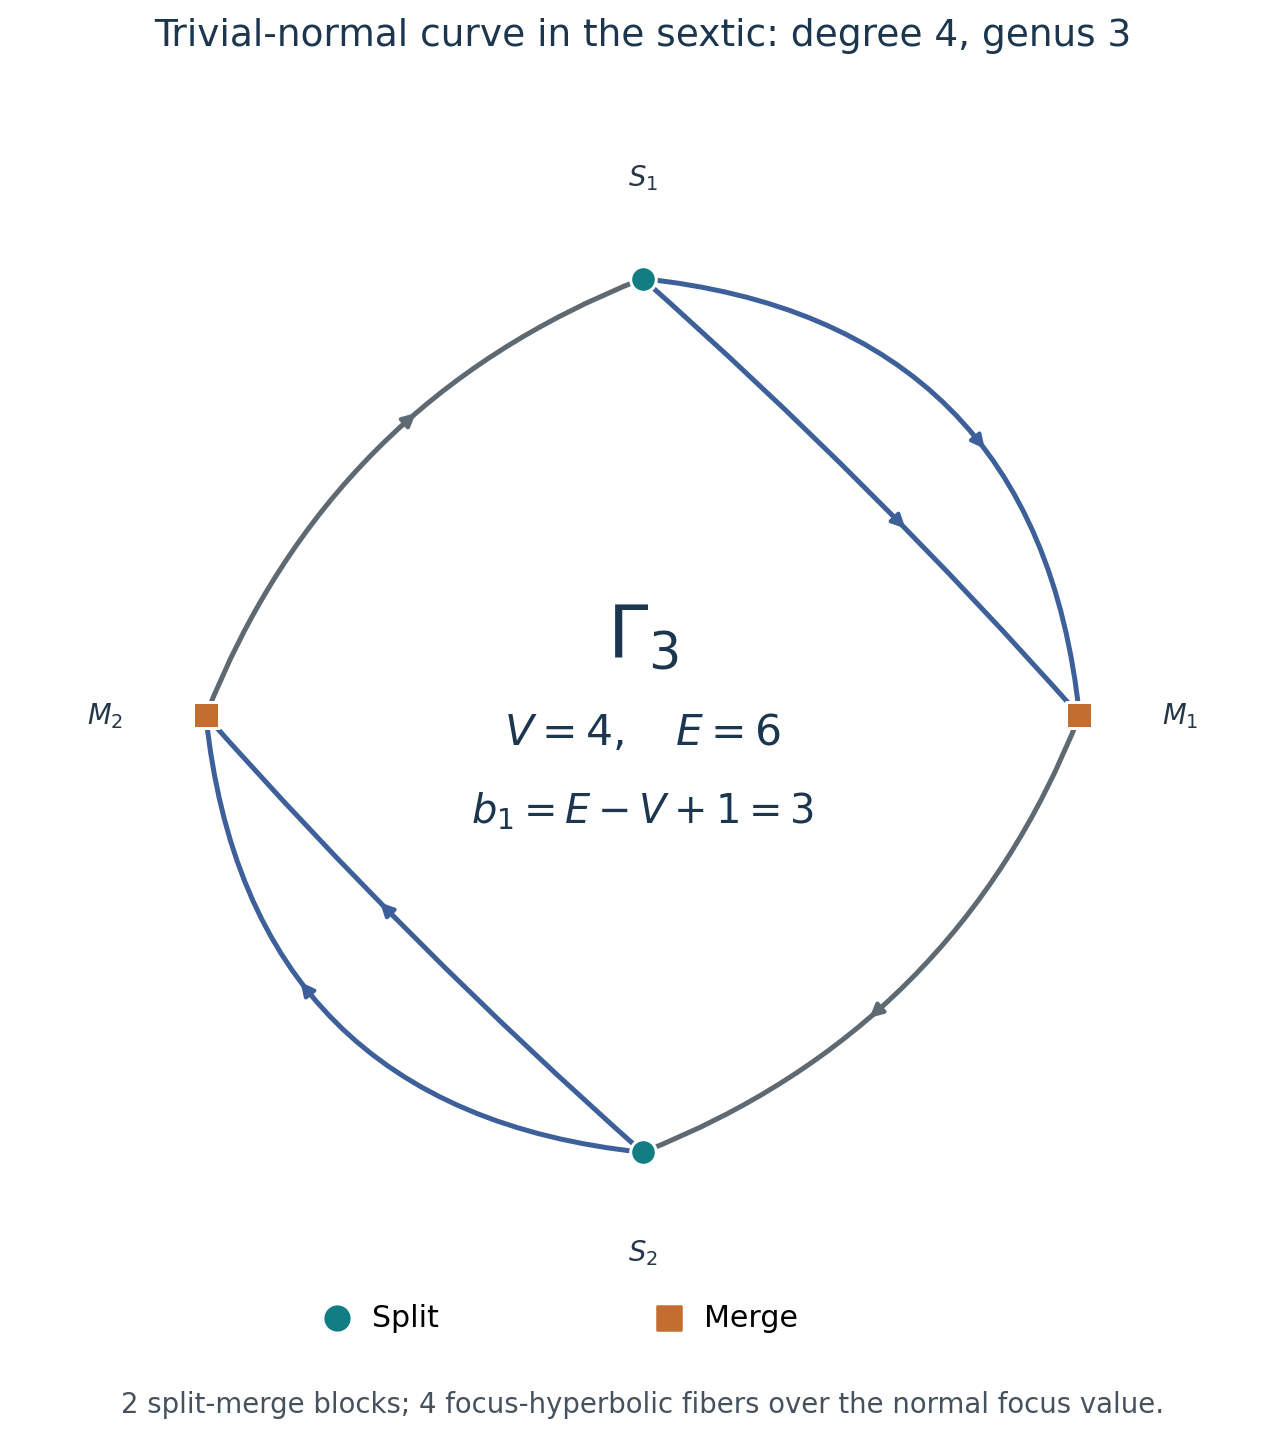
\includegraphics[width=0.73\textwidth]{trivial_normal_curve_graph.png}
 \caption{六次超曲面内の trivial-normal symplectic curve $C'$ に用いる genus-three Reeb graph。
 曲線は degree $4$、genus $3$ で、graph は4頂点・6辺・$b_1=3$を持つ。
 Actual base は $R\times\Gamma_3$ であり、normal focus value $o\in\operatorname{int}R$ と
 各 graph vertex の組の上に、Euler 数 $-1$ の whole focus--hyperbolic fiber がある。
 $\partial R$ の normal faces は残る。}
 \label{tnc:graph-figure}
\end{figure}

\begin{corollary}[残りの compact domain の Euler 数]\label{tnc:complement-euler}
上の $\mathcal U$ に対して
$\mathcal V=\overline{X_d\setminus\operatorname{int}\mathcal U}$ と置くと
\begin{equation}\label{tnc:complement-number}
 \chi(\mathcal V)
 =d(10-10d+5d^2-d^3)+(d-2)(d-5).
\end{equation}
特に六次では $\chi(\mathcal V)=-512$ である。
\end{corollary}

\begin{proof}
$\mathcal U\simeq C'\times K_c$ であり、$C'$ は closed なので
$\partial\mathcal U\simeq C'\times\partial K_c$ である。
$\partial K_c$ は corners を丸めれば closed oriented three-manifold となり、Euler 数は零である。
従って $\chi(\partial\mathcal U)=0$。
$\mathcal U$ の corners を小さい collar 内で丸める操作は、領域と complement の Euler 数を変えない。
丸めた collared boundary に沿って有限 CW 型の Euler 数の加法性を適用すると
\[
 \chi(X_d)=\chi(\mathcal U)+\chi(\mathcal V)-\chi(\partial\mathcal U)
          =-(d-2)(d-5)+\chi(\mathcal V).
\]
第\ref{bct:section}節の $\chi(X_d)$ の式を代入する。
\end{proof}

\begin{proposition}[補集合のEuler数が課すsingular fiber予算]
\label{tnc:complement-singularity-budget}
$d\ge6$ とし，系\ref{tnc:closed-block}の局所blockを
$\mathcal U\subset X_d$，そのcompact complementを$\mathcal V$とする．
次の正整数を置く：
\[
 \begin{split}
 \mathcal N_d:=-\chi(\mathcal V)
  &=d(d^3-5d^2+10d-10)-(d-2)(d-5)\\
  &=d^4-5d^3+9d^2-3d-10>0.
 \end{split}
\]
$\mathcal V$に，compact triangulable base $B_{\mathcal V}$への
proper continuous map
$f:\mathcal V\to B_{\mathcal V}$があり，
有限CW型のfiberを持つ有限stratificationに関して局所自明であると仮定する．
\emph{Euler数が非零のfiberが存在するbase pointsが有限集合
$S\subset B_{\mathcal V}$に限られる}なら，必ず
\[
 \boxed{\sum_{b\in S}\chi(f^{-1}(b))=-\mathcal N_d<0}
\]
を満たす．従ってその有限集合のfiberのEuler数がすべて
非負ということはあり得ない．
さらに，すべての$b\in S$に対して
$\chi(f^{-1}(b))=-1$なら
\[
 \boxed{|S|=\mathcal N_d}.
\]
特に$d=6$では$\mathcal N_6=512$である．
\end{proposition}
\begin{proof}
系\ref{tnc:complement-euler}によって
$\chi(\mathcal V)=-\mathcal N_d$である．
その符号は$d\ge6$で
$d(d^3-5d^2+10d-10)>(d-2)(d-5)$
から従う．実際
$d^3-5d^2+10d-10=
(d-2)(d^2-3d+4)-2$と書ける．

有限stratificationの各stratum $S_\alpha$での典型fiberを
$F_\alpha$とすると，compact支えEuler数の積公式と加法性から
\[
 \chi(\mathcal V)
   =\sum_\alpha
       \chi_c(S_\alpha)\,\chi(F_\alpha).
\]
ここで正次元stratumのcompact支えEuler数は負になり得るため，
\emph{全fiberのEuler数が非負}というだけでは
$\chi(\mathcal V)<0$に矛盾しないことに注意する．
本命題では$S$以外のfiberのEuler数が零なので，
それらのstrataの寄与は全て消え，
\[
 \chi(\mathcal V)=\sum_{b\in S}\chi(f^{-1}(b))
\]
となる．残る結論は直ちに従う．
\end{proof}

\begin{remark}[適用範囲と実際の課題]
この命題は\emph{仮に補集合の有限stratified fibrationが存在すれば}
生じる必要条件を与える．
一般のfiberには負以外のEuler数が生じてもよく，
Euler数が非零のfiberが正次元のbase stratumに並ぶ可能性もある．
従って全体のLagrangian fibrationに
$512$個の特定型fiberが必ず存在するとまでは主張しない．
現在構成済みの局所blockは$\chi(\mathcal U)=-(d-2)(d-5)$だけを担うので，
補集合の負のEuler数を説明するsingular strataを
別途設計しなければならない，という具体的な障害である．
\end{remark}

この $-512$ は、構成済みの actual domain を除いた compact complement の Euler 数である。
Complement 上の fibration はまだないため、残る singular fibers の個数とは解釈しない。

\subsection{管状補集合の整数ホモロジーと focus block との差}
\label{tnc:tubular-complement}

ここではEuler数だけでは見えない整数torsionと，
管状近傍とactual focus blockのtopologyの差を区別する．
$X_d$の三次元超曲面としての整数cohomologyについては
\cite[\S2.1]{randal-williams-hypersurface}のLefschetzおよび
Poincar\'e dualityの整理を用いる．

\begin{theorem}[閉曲線の管状補集合に現れるmeridional torsion]
\label{tnc:tubular-homology}
$d\ge6$ とし，$X_d\subset\mathbb P^4$をsmooth degree-$d$
hypersurface，$C\subset X_d$をdegree
$e=\langle\mathsf H,[C]\rangle>0$，genus $g$ の
connected closed embedded oriented surfaceとする．
そのoriented real rank-four normal disk bundleの
十分小さいclosed tubular neighborhoodを$N(C)$とし，
\[
 V_0=X_d\setminus\operatorname{int}N(C),\qquad
 b_d=d^4-5d^3+10d^2-10d+4
\]
とおく．以下は\emph{整数係数}のhomology群の同型である：
\begin{equation}\label{tnc:tubular-homology-groups}
\begin{aligned}
 H_0(V_0)&\simeq\mathbb Z,&
 H_1(V_0)&=0,&
 H_2(V_0)&\simeq\mathbb Z,\\
 H_3(V_0)&\simeq\mathbb Z^{b_d}\oplus\mathbb Z/e\mathbb Z,&
 H_4(V_0)&\simeq\mathbb Z^{2g},&
 H_k(V_0)&=0\quad(k\ge5).
\end{aligned}
\end{equation}
Normal $3$-sphere fiberのhomology classは
$H_3(V_0)$のtorsion summandを生成し，その位数は正確に$e$である．
特に定理\ref{tnc:actual-curve}のnormal-trivial curveでは
$e=d-2$であり，$d=6$なら
\[
 H_3(V_0;\mathbb Z)\simeq
       \mathbb Z^{520}\oplus\mathbb Z/4\mathbb Z,\qquad
 H_4(V_0;\mathbb Z)\simeq\mathbb Z^6,\qquad
 \chi(V_0)=-512.
\]
\end{theorem}
\begin{proof}
Lefschetzの超平面定理とPoincar\'e dualityにより
$H_1(X_d)=H_5(X_d)=0$，
$H_2(X_d)\simeq H_4(X_d)\simeq\mathbb Z$，
$H_3(X_d)\simeq\mathbb Z^{b_d}$が成り立つ．
ここで
\[
 b_d=4-\chi(X_d),\qquad
 \chi(X_d)=d(10-10d+5d^2-d^3)
\]
はChern類の計算で得られる．
Excisionとoriented codimension-fourのThom同型から
\begin{equation}\label{tnc:thom-pair}
 H_k(X_d,V_0;\mathbb Z)
 \simeq H_k(N(C),\partial N(C);\mathbb Z)
 \simeq H_{k-4}(C;\mathbb Z).
\end{equation}
対の長完全列の次数$4,3$の部分は
\[
 H_4(X_d)\xrightarrow{\;\iota_C\;}H_0(C)
 \xrightarrow{\;\partial\;}H_3(V_0)
 \longrightarrow H_3(X_d)\longrightarrow0.
\]
$H_4(X_d)$の生成元はhyperplane divisorの基本類であり，
$\iota_C$はその$C$との交点数を取る写像，
すなわち$\mathbb Z\xrightarrow{\times e}\mathbb Z$である．
従って
\[
 0\longrightarrow \mathbb Z/e\mathbb Z
 \longrightarrow H_3(V_0)
 \longrightarrow H_3(X_d)\longrightarrow0
\]
が得られる．$H_3(X_d)$は自由なので群としてsplitする．
$\partial(1)$はThom円板の境界であるnormal meridian
$S^3$を表し，その位数はちょうど$e$である．

また$H_5(X_d)=0$と
$H_5(X_d,V_0)\simeq H_1(C)=\mathbb Z^{2g}$より，
前の$\iota_C$の単射性を用いて
$H_4(V_0)\simeq H_1(C)$を得る．
同様に$H_3(X_d,V_0)=H_2(X_d,V_0)=0$より
$H_2(V_0)\simeq H_2(X_d)$，$H_1(V_0)=0$が従う．
次数$6,5$では
$H_6(X_d)\to H_6(X_d,V_0)\simeq H_2(C)$
が両者の基本類の対応による同型であることから
$H_5(V_0)=0$を得る．$V_0$は境界のあるcompact
six-manifoldなので$H_6(V_0)=0$である．
従って表示\eqref{tnc:tubular-homology-groups}を得る．
Euler数は
$2-b_d+2g=\chi(X_d)-(2-2g)$であり，六次では$-512$である．
\end{proof}

\begin{lemma}[Actual focus normal blockは円板ではない]
\label{tnc:focus-nondisk}
第\ref{fhr:section}節の
$K_c=G_c^{-1}(R)\subset\mathbb C^2$は
$H_1(K_c;\mathbb Z)$に$\mathbb Z$を直和因子として含む．
従って定理\ref{tnc:actual-curve}のclosed-curve block
$\mathcal U\simeq C'\times K_c$は，
通常の管状disk neighborhood
$C'\times D^4$とhomotopy equivalentではない．
\end{lemma}
\begin{proof}
$G_c=(P_X-P_Y,|XY-c|^2)$，
$R=[-a_*,a_*]\times[q_-,q_+]$であり
$0<q_-<c^2<q_+$である．
従って
\[
 \vartheta:K_c\longrightarrow S^1,\qquad
 (X,Y)\longmapsto\frac{XY-c}{|XY-c|}
\]
は連続である．$\sqrt{q_-}<r<c$を固定し，
$w(\theta)=c+r e^{i\theta}$と置く．
$w(\theta)\ne0$なので
\[
 X(\theta)=\sqrt{|w(\theta)|}>0,\qquad
 Y(\theta)=\frac{w(\theta)}{X(\theta)}
\]
は$K_c$内の閉曲線を定める：
$P_X-P_Y=0$，$|XY-c|^2=r^2\in(q_-,q_+)$である．
合成$\vartheta(X(\theta),Y(\theta))=e^{i\theta}$
は$S^1$のidentityだから
$\vartheta_*:H_1(K_c;\mathbb Z)\to\mathbb Z$は
split surjectiveである．
従って$H_1(K_c)$は$\mathbb Z$を直和因子に持つ．
一方$H_1(C'\times D^4)=H_1(C')$に対し
K\"unnethより$H_1(C'\times K_c)$には
$H_1(C')\oplus\mathbb Z$が直和因子として現れる．
両者の第一Betti数が異なるので同じhomotopy型ではない．
\end{proof}

\begin{proposition}[Focus block の境界torus bundleとmeridianの差]
\label{tnc:focus-boundary-homology}
$K_c$を補題\ref{fhr:focus-block}のfour-dimensional
focus blockとする．$\partial K_c$はcornersを丸めた後，
$S^1$上の$T^2$-bundleであり，fiberの一次homology上の
monodromyは適当なsymplectic integral basisで
\[
 M=\begin{pmatrix}1&1\\0&1\end{pmatrix}
\]
（基底とloopの向きによって逆または転置へ置換）である．
従って
\[
 H_1(\partial K_c;\mathbb Z)\simeq\mathbb Z^2,\quad
 H_2(\partial K_c;\mathbb Z)\simeq\mathbb Z^2,\quad
 H_3(\partial K_c;\mathbb Z)\simeq\mathbb Z.
\]
さらに$\partial K_c$の基本群は，fiberの生成元を$a,b$，
base loopを$t$とすると
\[
 \pi_1(\partial K_c)
 \simeq\langle a,b,t\mid[a,b]=1,\ 
            tat^{-1}=a,\ tbt^{-1}=ab\rangle
\]
であり，整数Heisenberg群と同型である．
この表示ではvanishing-cycle class $a=[t,b]$は
$H_1(\partial K_c;\mathbb Z)$で消えるが，
基本群では非自明である．
特に$\partial K_c$は$S^3$とhomology equivalentではなく，
closed curveに沿ったactual focus blockのnormal facesは
通常の管状disk bundleの$S^3$ facesにそのまま置換できない．
\end{proposition}
\begin{proof}
$G_c:K_c\to R$は中央$o$に一つだけ
nondegenerate focus--focus critical pointを持ち，
$\partial R$上ではregular torus fibersを持つ．
従って$\partial K_c=G_c^{-1}(\partial R)$はtorus bundleである．
一focus点の標準monodromy公式は
\cite[Section~3]{zung-focus-cf}によって
primitive unipotent transvection $M$ となる．
Wang長完全列において
\[
 H_1(T^2)=\mathbb Z^2,\quad H_2(T^2)=\mathbb Z,\qquad
 \operatorname{coker}(M-I)\simeq\mathbb Z,\quad
 \ker(M-I)\simeq\mathbb Z
\]
だから，$H_1(\partial K_c)$は
$\mathbb Z$と$\mathbb Z$のextensionであり$\mathbb Z^2$，
同じく$H_2(\partial K_c)\simeq\mathbb Z^2$．
Orientationで$H_3\simeq\mathbb Z$が従う．
またmapping torusのvan Kampen表示は
$\pi_1(T^2)\rtimes_M\mathbb Z$であり，上のrelationsになる．
$\langle a,b,t\rangle$のcommutatorは$a=[t,b]$で，
$a$は中心に属するため整数Heisenberg群の標準表示を得る．
\end{proof}

\begin{corollary}[Closed-curve focus face の整数Betti数]
\label{tnc:focus-boundary-betti}
定理\ref{tnc:actual-curve}のgenus-$g$ closed curve $C'$上の
product focus block $\mathcal U=C'\times K_c$の境界は，
cornersを丸めた後，$C'\times\partial K_c$と同相である．
その整数homologyはtorsion-freeで，
\[
 \bigl(b_0,b_1,b_2,b_3,b_4,b_5\bigr)
 =\bigl(1,\,2g+2,\,4g+3,\,4g+3,\,2g+2,\,1\bigr).
\]
さらに
\[
 \pi_1(\partial\mathcal U)
 \simeq\pi_1(C')\times H_{\mathbb Z}.
\]
特に$d=6$では$g=3$なので
\[
 (b_0,\ldots,b_5)=(1,8,15,15,8,1).
\]
\end{corollary}
\begin{proof}
$C'$はclosedであり$\mathcal U=C'\times K_c$だから
$\partial\mathcal U=C'\times\partial K_c$である．
命題\ref{tnc:focus-boundary-homology}から
$\partial K_c$の整数homologyは
$\mathbb Z,\mathbb Z^2,\mathbb Z^2,\mathbb Z$であり，
各次数でtorsionを持たない．
$H_*(C')=(\mathbb Z,\mathbb Z^{2g},\mathbb Z)$を用いる
K\"unneth formulaにより表示が得られる．
基本群はproductのvan Kampen定理による．
\end{proof}

\begin{lemma}[Normal focus domain のhomotopy型]
\label{tnc:focus-homotopy}
補題\ref{fhr:focus-block}の$K_c$は
\[
 K_c\simeq S^1\vee S^2,\qquad
 H^j(K_c;\mathbb Z)=
 \begin{cases}\mathbb Z&(j=0,1,2),\\0&(j\ge3).\end{cases}
\]
\end{lemma}
\begin{proof}
$w=XY$，$A=P_X-P_Y$とし，
$W=\{w:q_-\le|w-c|^2\le q_+\}$と書く．
$W$は$w=0$を内部に含むclosed annulusである．
$w$を固定したまま，$A$を$(1-s)A$へ変形する．
式\eqref{fhr:radii}によって，その都度
\[
 P_X(s)=\frac{\sqrt{(1-s)^2A^2+4\pi^2|w|^2}+(1-s)A}{2},
 \quad
 P_Y(s)=\frac{\sqrt{(1-s)^2A^2+4\pi^2|w|^2}-(1-s)A}{2}
\]
とし，$w\ne0$なら$X,Y$の位相を保つ．
$w=0$では非零の方の座標を$\sqrt{1-s}$倍して，
もう一方は零のままとする．これは$w=0$にも連続に延び，
$Q=|w-c|^2$を保持して$|A_s|\le a_*$なので，
$A=0$へのstrong deformation retractionを与える．

$A=0$では$|X|=|Y|=\sqrt{|w|}$であり，
$w\ne0$のfiberは$S^1$，$w=0$のfiberは一点となる．
従って
\[
 \{A=0\}\cong(W\times S^1)/(\{0\}\times S^1\text{ を潰す}).
\]
$W$を，$w=0$を固定して中央の円$\{|w-c|=c\}$
へradial deformation retractすると，右辺は
$(S^1\times S^1)/(\{*\}\times S^1)$とhomotopy equivalentである．
TorusのCW表示の一つの1-cellを潰すと，
二次cellのcommutator attaching wordは自明になるため，
$S^1\vee S^2$を得る．
\end{proof}

\begin{theorem}[Actual focus block補集合の整数homology]
\label{tnc:actual-complement-homology}
定理\ref{tnc:actual-curve}のclosed curve
$C'\subset X_d$について
$e=d-2$，$g=(d-3)(d-4)/2$，
$\mathcal U=C'\times K_c$，
$\mathcal V=\overline{X_d\setminus\operatorname{int}\mathcal U}$とおく．
$b_d=d^4-5d^3+10d^2-10d+4$とすれば
\begin{equation}\label{tnc:actual-complement-groups}
\begin{aligned}
 H_0(\mathcal V)&\simeq\mathbb Z,&
 H_1(\mathcal V)&\simeq\mathbb Z,&
 H_2(\mathcal V)&\simeq\mathbb Z^{2g+2},\\
 H_3(\mathcal V)&\simeq
  \mathbb Z^{b_d+2g+1}\oplus\mathbb Z/e\mathbb Z,&
 H_4(\mathcal V)&\simeq\mathbb Z^{2g+1},&
 H_k(\mathcal V)&=0\ (k\ge5).
\end{aligned}
\end{equation}
Torsion summandの生成元は，固定した$p\in C'$上の
focus normal face $\{p\}\times\partial K_c$の有向3-cycleである．
特に六次では
\[
 H_1(\mathcal V)=\mathbb Z,\quad
 H_2(\mathcal V)=\mathbb Z^8,\quad
 H_3(\mathcal V)=\mathbb Z^{527}\oplus\mathbb Z/4,\quad
 H_4(\mathcal V)=\mathbb Z^7,\quad
 \chi(\mathcal V)=-512.
\]
\end{theorem}
\begin{proof}
補題\ref{tnc:focus-homotopy}，K\"unnethより
$H^j(\mathcal U;\mathbb Z)$は$j=0,4$で$\mathbb Z$，
$j=1,3$で$\mathbb Z^{2g+1}$，
$j=2$で$\mathbb Z^{2g+2}$，他では零である．
Excisionと，cornersを丸めたcompact oriented
six-manifoldに対するPoincar\'e--Lefschetz双対性により
\[
 H_k(X_d,\mathcal V)\simeq
 H_k(\mathcal U,\partial\mathcal U)
 \simeq H^{6-k}(\mathcal U).
\]
この同型の下で$H_k(X_d)\to H_k(X_d,\mathcal V)$は
cohomologyの制限$H^{6-k}(X_d)\to H^{6-k}(\mathcal U)$に対応する．
$\mathcal U$は小さいnormal disk bundle
$N(C')\simeq C'$に含まれるので，次数3以上の制限は零である．
次数2ではhyperplane classの制限が
$H^2(\mathcal U)\simeq H^2(C')\oplus
(H^1(C')\otimes H^1(K_c))\oplus H^2(K_c)$
の第一因子に$e$倍で入る．

定理\ref{tnc:tubular-homology}で記した
$H_2(X_d)=H_4(X_d)=\mathbb Z$，
$H_3(X_d)=\mathbb Z^{b_d}$，
$H_1(X_d)=H_5(X_d)=0$を用いる．
次数4,3の長完全列は
\[
 0\to H^1(\mathcal U)\to H_4(\mathcal V)
 \to\mathbb Z\xrightarrow{\times e}H^2(\mathcal U)
 \to H_3(\mathcal V)\to\mathbb Z^{b_d}\to0
\]
となる．$\times e$は第一summandへの単射であり，
そのcokernelは$\mathbb Z^{2g+1}\oplus\mathbb Z/e$である．
$\mathbb Z^{b_d}$は自由なのでextensionは群としてsplitし，
$H_3,H_4$の表示を得る．
$\mathbb Z/e$の生成元は$H^2(C')$の基本classを
relative dualityで表す
$\{p\}\times[K_c,\partial K_c]$のboundary
$\{p\}\times\partial K_c$に対応する．
同様に次数3,2の制限が零なので
$H_2(\mathcal V)\simeq H^3(\mathcal U)\oplus\mathbb Z$
および$H_1(\mathcal V)\simeq H^4(\mathcal U)$が従う．
最上次数では$H_6(X_d)\to H^0(\mathcal U)$が同型で，
$H_k(\mathcal V)=0$ ($k\ge5$)を得る．
六次の数値とEuler数は式への代入である．
\end{proof}

\begin{proposition}[Focus base circuit はactual補集合の原始一次class]
\label{tnc:focus-boundary-primitive}
定理\ref{tnc:actual-complement-homology}の設定で，
normal focus map $G_c:K_c\to R$の境界
$\partial R\simeq S^1$を一周するloopを，
次のexplicit sectionで$\partial K_c$へ持ち上げる：
\[
 w=XY=c+\sqrt q>0,\quad
 X=\sqrt{P_X(A,w)/\pi}>0,\quad Y=w/X>0
 \qquad ((A,q)\in\partial R).
\]
このloopのclassを$t\in H_1(\partial K_c;\mathbb Z)$とする．
$C'$の基点$p$を固定すると
\[
 t_p=[\{p\}\times t]\in H_1(\partial\mathcal U;\mathbb Z)
\]
は$H_1(\partial\mathcal U)\to H_1(\mathcal U)$の
kernelを生成し，そのactual complementへの像は
\[
 H_1(\mathcal V;\mathbb Z)\simeq\mathbb Z
\]
の\emph{原始生成元}である（符号は向きによる）．
従って，global fillingを考える際，
normal focus base circuit を補集合側で
null-homologousにするような境界同定は不可能である．
\end{proposition}
\begin{proof}
補題\ref{tnc:focus-homotopy}の
$\vartheta:K_c\to S^1$，
$\vartheta(X,Y)=(XY-c)/|XY-c|$は
$H_1(K_c)\simeq\mathbb Z$のgeneratorを検出する．
$0<r<c$，$q_-<r^2<q_+$を固定し，
$\partial R$のface $A=a_*$上で
$w=c+r e^{i\theta}$と置く．
式\eqref{fhr:radii}によって$X>0$を選び
$Y=w/X$とすれば，このloopは
$\vartheta$の下でdegree oneとなる．
従って$H_1(\partial K_c)\to H_1(K_c)$は全射である．
命題\ref{tnc:focus-boundary-homology}により
$H_1(\partial K_c)\simeq\mathbb Z^2$だから，
そのkernelはrank oneのprimitive sublatticeである．

一方，表示したsectionは$R$全体へ延び，
$w-c=\sqrt q>0$なので$\vartheta$はsection上定数である．
従って$t$は$H_1(K_c)$で零である．
また$G_{c*}(t)$は
$H_1(\partial R)\simeq\mathbb Z$のgeneratorなので
$t$は$H_1(\partial K_c)$でprimitiveである．
ゆえに$t$がkernelを生成する．
$\partial\mathcal U=C'\times\partial K_c$と
$\mathcal U=C'\times K_c$にK\"unnethを用いると，
$H_1(\partial\mathcal U)\to H_1(\mathcal U)$は全射で，
kernelは$\mathbb Z\,t_p$である．

最後に$X_d=\mathcal U\cup\mathcal V$の
Mayer--Vietoris長完全列を用いる．
$H_1(X_d)=0$だから
\[
 H_1(\partial\mathcal U)
 \longrightarrow H_1(\mathcal U)\oplus H_1(\mathcal V)
 \longrightarrow H_1(X_d)=0
\]
の左の写像は全射である．
$H_1(\mathcal V)=\mathbb Z$は
定理\ref{tnc:actual-complement-homology}で計算済みなので，
$H_1(\mathcal U)$で零となるkernel generator $t_p$の
補集合側の像は$\pm1$でなければならない．
\end{proof}

\begin{remark}[管状補集合とactual focus補集合の比較]
\label{tnc:complement-distinction}
定理\ref{tnc:tubular-homology}の$V_0$と
定理\ref{tnc:actual-complement-homology}の$\mathcal V$は異なる．
いずれも$H_3$に位数$e=d-2$のtorsionを持つが，
\emph{自由部分と低次homologyは異なる}：
\[
 \begin{aligned}
 H_1(V_0)&=0,& H_1(\mathcal V)&\simeq\mathbb Z,\\
 \operatorname{rank}H_3(V_0)&=b_d,&
 \operatorname{rank}H_3(\mathcal V)&=b_d+2g+1 .
 \end{aligned}
\]
同じEuler数$\chi(V_0)=\chi(\mathcal V)$だけでは
これらの群は求められない．
差を支えるのは$K_c\simeq S^1\vee S^2$という局所topologyである．
第\ref{tnc:exterior-topology}節では具体的な Hopf 商を使い，
$\partial\mathcal U\to\mathcal U,\mathcal V$ の全整数 homology と
基本群の包含写像を決定する．
一方，action periods，Maslov data，coorientation と whole boundary foliation の
整合性，および relative Lagrangian filling は引き続き構成課題である．
なお$\mathbb Z/(d-2)$の補集合のtorsionと，
\cite[\S2.1]{randal-williams-hypersurface}に現れる
ambient $\pi_3(X_d)$の$\mathbb Z/d$は別の不変量である．
\end{remark}

\paragraph{閉還元面の収支との整合.}
$\nu=\mathfrak a/(d-5)$ とすれば
\[
 \operatorname{Area}(C')+\nu\chi(C')
 =(d-2)\mathfrak a-\frac{\mathfrak a}{d-5}(d-2)(d-5)=0.
\]
従って closed reduction の section が存在する場合の面積条件とも整合する。
Generic plane section $C$ の normal degree $2d$ を零へ変えたわけではなく、
degree と genus の異なる $C'$ を選んでいる。

\paragraph{大域化との距離.}
この結果は、所定の $X_d$ の actual symplectic form の下で、閉曲線全体を含む
non-elliptic focus--hyperbolic block を与える。
既存 shell の fiber relation、指定された旧 annular germs、旧48 ports の接続は保持していない。
$\partial R\times\Gamma$ の接続、残りの $X_d$ の被覆、および global base における graph cycles の処理は未構成である。
従って境界を持たない全体 fibration の存在は、引き続き未証明である。

% !TeX root = ../../../threefold-lagrangian-torus-fibration.tex
% 2026-11-21 / v1.0
\section{Actual focus 補集合の境界写像と被覆空間}
\label{tnc:exterior-topology}

以下は，定理\ref{tnc:actual-curve}の曲線と，
補題\ref{fhr:focus-block}の具体的な normal focus domain に対する結果である．
整数 homology の群を列挙するだけでなく，両側の包含写像と
補集合の fundamental group を求める．
標準の nodal 模型は Auroux \cite[Section~5.1]{auroux-local} に現れ，
四次元の fishtail 自体とその補集合を調べる考え方には，
例えば $S^4$ の二つの fishtails への分解
\cite[Introduction and Figure~1]{akbulut-double-fishtail}が先行する．
ここではその diffeomorphism や symplectic gluing を借用せず，
指定された埋込みの Hopf 商を直接使う．
Homotopy 長完全列・Hopf bundle・Hurewicz theorem は
\cite[Theorems~4.32 and 4.41, Example~4.45]{hatcher-bct}の標準的な入力である．
以下の具体的な境界表示と被覆計算について包括的な新規性確認は未了である．

\subsection{Hopf 商による actual 補集合の基本群}
\label{tnc:focus-complement-pi1-section}

ここでは $K_c$ の abstract な homotopy 型だけでなく，
式\eqref{fhr:focus-map}による $\mathbb C^2$ 内の具体的な埋込みを使う．
この情報により，前節で求めた $H_1(\mathcal V)=\mathbb Z$ を
基本群の計算へ強められる．すべての corners は必要に応じて
小さい collar 内で丸める．この操作は以下の基本群と包含写像を変えない．

\begin{lemma}[Focus normal exterior の Hopf 商]
\label{tnc:focus-exterior-hopf}
$K_c\subset\operatorname{int}D^4_\rho\subset\mathbb C^2$ となる
closed round ball を取り，
\[
 E=D^4_\rho\setminus\operatorname{int}K_c,
 \qquad Y=\partial K_c
\]
とおく．このとき $\pi_1(E)\simeq\mathbb Z$ である．
また $Y$ の normal circle を $a$，
$XY-c$ の位相を一周する complementary fiber circle を $b$，
命題\ref{tnc:focus-boundary-primitive}の positive-real section による
focus base boundary circuit を $t$ とすると，適当な基点への経路を選んで
\[
 \pi_1(Y)\longrightarrow\pi_1(E)=\langle\tau\rangle,
 \qquad a\longmapsto1,\quad b\longmapsto1,
 \quad t\longmapsto\tau
\]
とできる．$\tau$ の向きは $t$ により定める．
\end{lemma}

\begin{proof}
逆位相の作用
\[
 z\cdot(X,Y)=(zX,z^{-1}Y),\qquad z\in S^1,
\]
の商写像を
\[
 h:\mathbb C^2\longrightarrow\mathbb R\times\mathbb C,
 \qquad h(X,Y)=(A,w),\quad
 A=\pi(|X|^2-|Y|^2),\quad w=XY
\]
とする．式\eqref{fhr:radii}により $(A,w)$ は各 orbit を一意に定め，
原点以外の orbit は自由な $S^1$ である．
特に $h$ は $\mathbb C^2/S^1\simeq\mathbb R^3$ を与え，
原点を除けば principal circle bundle である．
さらに
\[
 A^2+4\pi^2|w|^2
   =\pi^2(|X|^2+|Y|^2)^2
\]
なので $D^4_\rho$ の商は ellipsoid
\[
 D=\{(A,w):A^2+4\pi^2|w|^2\le\pi^2\rho^4\}
\]
であり，$h:\partial D^4_\rho\to\partial D$ は Hopf bundle である．
これは第二複素座標を共役にした通常の Hopf 写像であり，
Euler 数の絶対値は一である．

$r_\pm=\sqrt{q_\pm}$ とおくと
\[
 \mathcal Q=[-a_*,a_*]\times
       \{w:r_-\le|w-c|\le r_+\},\qquad
 K_c=h^{-1}(\mathcal Q).
\]
$\mathcal Q$ は $D$ の内部にある unknotted solid torus である．
実際 $(A,r,\theta)\mapsto(A,c+r e^{i\theta})$ により
rectangle $[-a_*,a_*]\times[r_-,r_+]$ と $S^1$ の積であり，
core は平面 $A=0$ 内の丸い円として選べる．
$r_-<c<r_+$ だから $(A,w)=(0,0)$ はその内部にある．
従って
\[
 B=D\setminus\operatorname{int}\mathcal Q,
 \qquad h:E\longrightarrow B
\]
は fixed point を持たない principal circle bundle である．
$D$ の外側に ball を付けて $S^3$ と見ると，
unknotted solid torus の exterior も solid torus である．
従って $B$ は solid torus から open three-ball を除いたものと同相であり，
\[
 \pi_1(B)\simeq\mathbb Z.
\]
その原始生成元は $\mathcal Q$ の meridian である．

Bundle の homotopy 長完全列から
\[
 \pi_1(S^1)\longrightarrow\pi_1(E)
       \xrightarrow{h_*}\pi_1(B)\longrightarrow1
\]
は完全である．Fiber circle を $B$ 内の経路に沿って
outer boundary $\partial D$ まで運ぶと，その移送先は
$h^{-1}(\partial D)=S^3$ 内の Hopf fiber である．
$S^3$ は単連結なので，この orbit は $E$ 内で null-homotopic である．
従って左の写像は零であり，$h_*$ は同型になる．
同じことは outer $S^2$ に対する connecting map
$\pi_2(B)\to\pi_1(S^1)$ が Hopf Euler 数 $\pm1$ により
全射となることからも従う．

残る境界写像は商空間で直接読める．$a$ は $h$ の fiber なので消える．
$r_-<r<c$ を固定し，face $A=a_*$ で
\[
 w(\theta)=c+r e^{i\theta},\qquad
 X(\theta)=\sqrt{P_X(a_*,w(\theta))/\pi}>0,
 \quad Y(\theta)=w(\theta)/X(\theta)
\]
と取った $b$ は $\mathcal Q$ の longitude へ写る．
この longitude は $A=a_*+\delta$ へ少し押し出し，
その平面内の円板 $|w-c|\le r$ で埋められる．
$\mathcal Q\Subset\operatorname{int}D$ と $D$ の凸性により，
十分小さい $\delta>0$ ならこの円板と押出しは $B$ 内に取れる．
従って $h_*(b)=1$ であり，$b$ も $E$ で消える．
一方 $t$ は
\[
 w=c+\sqrt q>0,\quad
 X=\sqrt{P_X(A,w)/\pi}>0,\quad Y=w/X>0,
 \qquad (A,q)\in\partial R
\]
で与えられるので，$h(t)$ は $\theta=0$ における
rectangle $[-a_*,a_*]\times[r_-,r_+]$ の境界である．
すなわち $\mathcal Q$ の meridian を一周する．
これが $\pi_1(B)$ の原始生成元なので結論を得る．
\end{proof}

\begin{proposition}[Normal exterior の homotopy 型]
\label{tnc:focus-exterior-homotopy}
補題\ref{tnc:focus-exterior-hopf}の $E$ は
\[
 \boxed{E\simeq S^1\vee S^2\vee S^3}
\]
を満たす．この同値で $S^1$ の正の生成元は $t$ の像に選べる．
従って $\Lambda=\mathbb Z[\tau,\tau^{-1}]$ とすると，
universal cover $\widetilde E$ の deck action を伴う homology は
\[
 H_1(\widetilde E;\mathbb Z)=0,\qquad
 H_2(\widetilde E;\mathbb Z)\simeq\Lambda,
 \qquad H_3(\widetilde E;\mathbb Z)\simeq\Lambda.
\]
また inclusion $\partial D^4_\rho=S^3\hookrightarrow E$ は，
上の $S^3$ summand の inclusion に対応するよう選べる．
\end{proposition}

\begin{proof}
前補題の $B$ は solid torus から interior three-ball を除いたものである．
Sphere collar に一本の three-dimensional $1$-handle を付ける表示を取り，
その handle を core arc に縮めると，$B$ は outer sphere $\partial D$
と，その二点を結ぶ一本の arc の和へ homotopy equivalent になる．
Arc の両端を sphere 内の経路に沿って同じ基点に移せば，
pair として
\[
 (B,\partial D)\simeq(S^2\vee S^1,S^2)
\]
を得る．ここで $S^1$ の生成元は $\mathcal Q$ の meridian に取る．
特に $S^2$ への制限が $\partial D$ の parametrization である
homotopy equivalence $j:S^2\vee S^1\to B$ を選べる．

Principal circle bundle $E\to B$ を $j$ で引き戻した全空間を $P$ とする．
Pullback の map $P\to E$ は各 fiber 上の identity を与える．
両 bundle の homotopy 長完全列と $j$ の homotopy equivalence を用いれば，
これはすべての homotopy groups に同型を誘導する．
両全空間は CW 型を持つので，Whitehead の定理により
$P\to E$ は homotopy equivalence である．
その $S^2$ 上の部分は Euler 数 $\pm1$ の Hopf bundle で，全空間は $S^3$，
$S^1$ 上の部分は trivial bundle で，全空間は $S^1_a\times S^1_t=T^2$ である．
Wedge point 上では両者の同じ fiber circle を同定する．従って
\[
 P=S^3\cup_{S^1_a}T^2.
\]
双方への fiber inclusions は cofibrations なので，これは homotopy pushout でもある．
$S^1_a\to S^3$ は null-homotopic であるから，この arrow を定数写像へ変えても
homotopy pushout の homotopy 型は変わらない．よって
\[
 P\simeq S^3\vee(T^2/S^1_a).
\]
この同値は $S^3$ 側の構造写像を保つ homotopy pushout の比較として取れる．
$T^2$ の CW 表示で $1$-cells を $a,t$，$2$-cell の attaching word を
$ata^{-1}t^{-1}$ とする．Subcomplex $S^1_a$ を潰すと，
残る attaching loop は $tt^{-1}$ で null-homotopic だから
\[
 T^2/S^1_a\simeq S^1_t\vee S^2.
\]
これで所要の wedge 分解と outer $S^3$ の主張を得る．

$S^1\vee S^2\vee S^3$ の universal cover は，
整数で添字を付けた直線上の各頂点に $S^2$ と $S^3$ を一つずつ付けた CW complex である．
Deck generator $\tau$ は添字を一つ進める．
従って次数 $2,3$ の cellular homology はそれぞれ自由 rank-one
$\Lambda$-module であり，次数 $1$ の homology は零である．
\end{proof}

\begin{theorem}[Actual focus 補集合の基本群と両側の境界写像]
\label{tnc:actual-complement-pi1}
定理\ref{tnc:actual-complement-homology}の設定で，
\[
 \mathcal U=C'\times K_c\subset X_d,
 \qquad
 \mathcal V=\overline{X_d\setminus\operatorname{int}\mathcal U}
\]
とする．この具体的な product block の補集合は
\[
 \boxed{\pi_1(\mathcal V)\simeq\mathbb Z}
\]
を満たす．$\pi_1(\mathcal U)\simeq\pi_1(C')\times\langle b\rangle$，
$\pi_1(\partial\mathcal U)\simeq\pi_1(C')\times H_{\mathbb Z}$
という既存の同定の下で，両側への包含写像は
\[
\begin{array}{c|cc}
 &\pi_1(\mathcal U)&\pi_1(\mathcal V)=\langle\tau\rangle\\ \hline
 \gamma\in\pi_1(C')&(\gamma,1)&1\\
 a&(1,1)&1\\
 b&(1,b)&1\\
 t&(1,1)&\tau
\end{array}
\]
で与えられる．基点の変更による共役を除き，$a,b,t$ は
補題\ref{tnc:focus-exterior-hopf}で指定した実際の loops である．
特に二つの包含写像を合わせた準同型の kernel は
normal vanishing circle が生成する central subgroup
$\langle a\rangle\simeq\mathbb Z$ である．
\end{theorem}

\begin{proof}
系\ref{tnc:closed-block}で使った product neighborhood の内部で
$K_c\Subset\operatorname{int}D^4_\rho$ となる ball を選ぶ．
対応する通常の tubular neighborhood を
$N=C'\times D^4_\rho$，その補集合を
$V_0=\overline{X_d\setminus\operatorname{int}N}$ とすれば，
collars を入れた意味で
\[
 \mathcal V=V_0\cup_{C'\times S^3}(C'\times E)
\]
である．

Lefschetz の定理から $X_d$ は単連結である．
さらに実余次元四の smooth surface $C'\subset X_d$ を除いても
基本群は変わらない．実際 $X_d\setminus C'$ の任意の loop を
$X_d$ 内の円板で埋め，境界を固定した相対一般位置により
その円板を $C'$ と横断的にできる．
$2+2<6$ なので交わりは空である．
よって $X_d\setminus C'$ は単連結で，
normal radial retraction により homotopy equivalent な $V_0$ も単連結である．

補題\ref{tnc:focus-exterior-hopf}より
$\pi_1(C'\times E)=\pi_1(C')\times\mathbb Z$ である．
Intersection $C'\times S^3$ の基本群は $\pi_1(C')$ であり，
$C'\times E$ 側へは第一因子として入り，$V_0$ 側へは自明に写る．
従って van Kampen の定理により
\[
 \pi_1(\mathcal V)
 =\bigl(\pi_1(C')\times\mathbb Z\bigr)
      /\langle\!\langle\pi_1(C')\rangle\!\rangle
 \simeq\mathbb Z.
\]
同時に $\gamma,a,b,t$ の $\mathcal V$ 側の像も得られる．

$\mathcal U$ 側については $C'$ 因子の写像は identity である．
補題\ref{tnc:focus-homotopy}により $\pi_1(K_c)=\mathbb Z$ で，
$\vartheta=(XY-c)/|XY-c|$ はその同型を与える．
上で指定した $b$ の $\vartheta$-degree は一だから生成元である．
$a$ は $\vartheta$ の下で定数であるので消え，
$t$ は表示した positive-real section が $R$ 全体へ延びるので消える．
これで表を得る．

最後に
\[
 H_{\mathbb Z}
 =\langle a,b,t\mid[a,b]=[a,t]=1,\ [t,b]=a\rangle
\]
（向きにより $a$ を逆にする）では，$a$ を殺した商は
$\mathbb Z b\oplus\mathbb Z t$ であり，kernel は
central subgroup $\langle a\rangle$ そのものである．
$C'$ 因子は $\mathcal U$ 側に忠実に残るため，
両側への同時写像にもこれ以外の kernel はない．
\end{proof}

\begin{remark}[Filling に対する基本群の必要条件]
\label{tnc:pi1-filling-constraint}
この計算は abstract な $S^1\vee S^2$ の任意の埋込みに対する主張ではない．
Actual block の Hopf 商と，normal disk bundle の内部での product 埋込みを使っている．
従ってこの boundary marking を保つ relative filling では，
focus base circuit $t$ は補集合の基本群の生成元として残り，
曲線方向の loops と normal fiber の $a,b$ は消えなければならない．
特に $t$ を補集合内の円板で閉じるような候補は排除される．
一方，この必要条件と前節の homology 条件を満たすことだけでは，
所定の作用周期・Maslov data・whole boundary foliation を保つ
Lagrangian filling の存在は従わない．
\end{remark}

\subsection{Focus face の全整数境界写像}
\label{tnc:boundary-maps-section}

この節では，normal framing を固定した actual product embedding
$\mathcal U=C'\times K_c\subset N=C'\times D^4\subset X_d$
に対し，両側の境界包含が誘導する整数homology写像を決定する．
群の階数だけでなく，regular torus，そのvanishing cycleのtransport，
normal meridianの像を区別する．全てのhomologyは整数係数とする．

$Y=\partial K_c$，$E=\overline{D^4\setminus\operatorname{int}K_c}$，
$\mathcal V_0=\overline{X_d\setminus\operatorname{int}N}$ とおく．
Cornersを丸めると
\[
 \mathcal V=\mathcal V_0\cup_{C'\times S^3}(C'\times E),
 \qquad \partial\mathcal U=C'\times Y.
\]
$Y$の向きは$K_c$からの境界向きとし，$E$のouter sphereの向きを
$[S^3]=[Y]\in H_3(E)$となるよう固定する．

\begin{lemma}[Normal face のmarked生成元と二つの包含]
\label{tnc:normal-boundary-maps}
命題\ref{tnc:focus-boundary-homology}の生成元を，次のように選べる．
$a$は逆位相normal circleのorbit，$b$はregular torus内で
$\vartheta=(XY-c)/|XY-c|$のdegreeが一となるloop，
$t$は命題\ref{tnc:focus-boundary-primitive}のpositive-real sectionによる
focus base boundary circuitである．
$F$をregular torusの基本類，$T$を同sectionの上で$a$をtransportした
torusの基本類とすると
\[
 H_1(Y)=\mathbb Z b\oplus\mathbb Z t,
 \qquad H_2(Y)=\mathbb Z F\oplus\mathbb Z T,
 \qquad H_3(Y)=\mathbb Z[Y].
\]
$H_1(K_c)=\mathbb Z\beta$，$H_2(K_c)=\mathbb Z\sigma$および
\[
 H_1(E)=\mathbb Z\mu,\qquad H_2(E)=\mathbb Z\nu,
 \qquad H_3(E)=\mathbb Z\zeta
\]
の向きを適切に選ぶと，二つの包含写像は
\[
\begin{array}{c|cc}
 \text{cycle on }Y & H_*(K_c)&H_*(E)\\ \hline
 b&\beta&0\\
 t&0&\mu\\
 F&\sigma&0\\
 T&0&\nu\\
 {[Y]}&0&\zeta
\end{array}
\]
となる．$E$は連結で，$H_k(E)=0$ ($k\ge4$)である．
\end{lemma}

\begin{proof}
$Y\to\partial R$のWang列において，$F$は
$H_2(T^2)$からのprimitiveな像である．
Normal orbit $a$はmonodromy不変であり，positive-real sectionに沿う
orbit torus $T$はWang列の
$H_2(Y)\to\ker(M-I:H_1(T^2)\to H_1(T^2))=\mathbb Z a$
で$a$へ写る．従って$(F,T)$は整数基底である．
$H_1$の$(b,t)$も同じWang列の整数基底である．

Positive-real sectionは$R$全体に延びるので，$t$は$K_c$で消える．
同sectionの各点にnormal circleを作用させる写像
$S^1\times R\to K_c$は，$XY=c+\sqrt q>0$のため退化せず，
境界が$T$となるsolid torusを与える．従って$T$も$K_c$で消える．
$b$は$\vartheta$のdegree一のloopなので$\beta$の生成元へ写る．

$F,b$の$E$での消滅を，具体的なchainで確認する．
$\sqrt{q_-}<r<c$を固定し，face $A=a_*$，$Q=r^2$上のtorusを$F$に取る．
$\delta>0$を十分小さくし，$A=a_*+\delta$を固定して
\[
 w=c+\rho e^{i\theta},\qquad 0\le\rho\le r,
 \qquad
 X=\sqrt{P_X(A,w)/\pi}>0,\qquad Y=w/X
\]
とおく．$w\ne0$であり，$A>a_*$なのでこのdiskは$E$に入る．
その境界は$b$を$E$へ押し出したloopである．
さらにnormal circleを作用させると$S^1\times D^2$が得られ，
その境界は$F$の押出しとなる．従って$b,F$は$E$で零である．
全chainは，$K_c$を含むround ballに余裕を持たせ，$\delta$を小さくすれば
同じ$D^4$内に取れる．実際，$|w|\le c+r<c+\sqrt{q_+}$だからである．

補題\ref{tnc:focus-homotopy}のretractionで，$F$はpinched torusへ
写り，その二次基本類を生成する．従って$F\mapsto\sigma$である．
最後に$D^4=K_c\cup_Y E$のMayer--Vietoris列を用いる．
$H_3(Y)\to H_3(K_c)\oplus H_3(E)$，
$H_2(Y)\to H_2(K_c)\oplus H_2(E)$，
$H_1(Y)\to H_1(K_c)\oplus H_1(E)$はいずれも同型である．
上で求めた零の像と整数基底を代入すると，$t,T,[Y]$の$E$での像が
それぞれの群のprimitive生成元となる．
次数零の列から$E$は連結であり，境界を持つcompact四次元多様体なので
$H_k(E)=0$ ($k\ge4$)である．
最後に$\partial E=S^3\sqcup(-Y)$から$[S^3]=[Y]=\zeta$を得る．
\end{proof}

\begin{proposition}[Actual補集合の局所・管状分解]
\label{tnc:complement-product-splitting}
$e=d-2$，$g=(d-3)(d-4)/2$，
$\mathsf L=H_1(C')$，$u=[C']\in H_2(C')$とおく．
包含$\mathcal V_0\to\mathcal V$は全整数homology上で単射であり，
固定したproduct framingに対して加法的な分解
\[
 H_k(\mathcal V)\simeq H_k(\mathcal V_0)
 \oplus \bigl(H_{k-1}(C')\otimes\mathbb Z\mu\bigr)
 \oplus \bigl(H_{k-2}(C')\otimes\mathbb Z\nu\bigr)
\]
が成立する．負次数の群は零とする．
これはhomology群の分解であり，空間の積分解やhomotopy分解ではない．

$h\in H_2(\mathcal V_0)\simeq\mathbb Z$を
$H_2(X_d)$の正の生成元へ写る生成元とする．
また$m\in H_3(\mathcal V_0)$をnormal meridian $S^3$のclass，
$\ell_x\in H_4(\mathcal V_0)$を$x\in\mathsf L$に沿うnormal sphereのclassとする．
すると
\[
 \operatorname{ord}(m)=e,
 \qquad \mathsf L\xrightarrow{\;x\mapsto\ell_x\;}H_4(\mathcal V_0)
 \quad\text{は同型}
\]
であり，$C'\times E$のK\"unneth classのうち
\[
 u\otimes1\longmapsto eh,\quad
 x\otimes1\longmapsto0,\quad
 1\otimes\zeta\longmapsto m,\quad
 x\otimes\zeta\longmapsto\ell_x,\quad
 u\otimes\zeta\longmapsto0
\]
となる．$\mu,\nu$の因子は表示した新しい直和因子へ恒等的に入る．
\end{proposition}

\begin{proof}
$S^3\to E$は次数零と三で同型を誘導する．
全homologyがtorsion-freeなのでK\"unneth公式から
\[
 H_k(C'\times S^3)\longrightarrow H_k(C'\times E)
\]
は各次数でsplit injectionであり，cokernelは
$H_{k-1}(C')\otimes\mathbb Z\mu\oplus
H_{k-2}(C')\otimes\mathbb Z\nu$である．
従って$\mathcal V=\mathcal V_0\cup(C'\times E)$の
Mayer--Vietoris列のconnecting mapは全次数で零となる．
そのcokernel表示は$H_k(\mathcal V_0)$と上記二因子の直和を与える．

$C'\times\{p\}\subset C'\times S^3$は$X_d$内で$C'$とhomologousであり，
hyperplane degreeが$e$なので，$H_2(\mathcal V_0)\to H_2(X_d)$の同型の下で
$eh$を表す．次数一の像は$H_1(\mathcal V_0)=0$により零である．
Normal sphereの位数と$x\mapsto\ell_x$の同型は
定理\ref{tnc:tubular-homology}のThom長完全列のconnecting mapそのものである．
最後に$H_5(\mathcal V_0)=0$だから$u\otimes\zeta$の像も零である．
\end{proof}

\begin{theorem}[両側への全整数境界包含写像]
\label{tnc:all-boundary-homology-maps}
上の記号を用いる．$j_U:C'\times Y\to\mathcal U$，
$j_V:C'\times Y\to\mathcal V$の全正次数整数homology写像は
次の表で与えられる．$x$は$\mathsf L$の任意の元を動き，
tensor記号と固定した点の因子は省略する．
\[
\begin{array}{c|c|c|c}
 k& H_k(C'\times Y)\text{ の生成元}&(j_U)_*&(j_V)_*\\ \hline
1&x&x&0\\
 &b&\beta&0\\
 &t&0&\mu\\ \hline
2&u&u&eh\\
 &xb&x\beta&0\\
 &xt&0&x\mu\\
 &F&\sigma&0\\
 &T&0&\nu\\ \hline
3&ub&u\beta&0\\
 &ut&0&u\mu\\
 &xF&x\sigma&0\\
 &xT&0&x\nu\\
 &[Y]&0&m\\ \hline
4&uF&u\sigma&0\\
 &uT&0&u\nu\\
 &x[Y]&0&\ell_x\\ \hline
5&u[Y]&0&0
\end{array}
\]
次数零では両包含とも同型である．特に
\[
 \operatorname{coker}\bigl((j_V)_*:H_2(C'\times Y)\to H_2(\mathcal V)\bigr)
 \simeq\mathbb Z/e\mathbb Z,
\]
また
\[
 \frac{H_3(\mathcal V)}{(j_V)_*H_3(C'\times Y)}\simeq H_3(X_d),
 \qquad
 (j_V)_*:H_4(C'\times Y)\twoheadrightarrow H_4(\mathcal V).
\]
従ってnormal faceの基本三次classは補集合の位数$e$のtorsionへ写り，
regular torus $F$とvanishing-cycle transport torus $T$は，
二つの側で異なるprimitive classを担う．
\end{theorem}

\begin{proof}
$j_U=\operatorname{id}_{C'}\times(Y\to K_c)$なので，
その列は補題\ref{tnc:normal-boundary-maps}とK\"unneth公式から得られる．
$j_V$は$C'\times Y\to C'\times E\to\mathcal V$へ分解し，
補題\ref{tnc:normal-boundary-maps}および
命題\ref{tnc:complement-product-splitting}を順に適用すれば右列となる．
次数二の像は$eh$と全ての$x\mu,\nu$で生成されるのでcokernelは$\mathbb Z/e$．
次数三の像は$\mathbb Z/e\langle m\rangle$と
$\mathsf L\otimes\mathbb Z\nu\oplus\mathbb Z u\mu$からなり，
残る商はThom列によって$H_3(X_d)$である．
次数四の像は$\ell_x,u\nu$で全体を生成する．
\end{proof}

\begin{remark}[非標準的なsplittingと未決定事項]
\label{tnc:boundary-maps-scope}
上の記述ではnormal framing，marked loops，orientationを固定した．
$H_3(\mathcal V_0)$を
$\mathbb Z^{b_d}\oplus\mathbb Z/e$と書く際の
$H_3(X_d)$のliftは一般に非標準的であるが，torsion subgroup，
$m$の像および表の境界像にこの選択は不要である．
また，表は所定のactual embeddingに対する整数homologyの必要条件であり，
作用周期，Maslov data，reduced foliation，relative symplectic fillingの
存在を結論しない．特にhomology写像を合わせただけで
Lagrangian fibrationを接着できるとは主張しない．
\end{remark}

\subsection{Focus 補集合の第二ホモトピー群と有限巡回被覆}
\label{tnc:equivariant-pi2-section}

引き続き $C=C^\prime$ とする．
定理\ref{tnc:actual-complement-pi1}の積管状近傍を $N=C\times D^4$ とし，
actual focus block を $\mathcal U=C\times K_c\subset\operatorname{int}N$ とする．
\[
 V_0=\overline{X_d\setminus\operatorname{int}N},\qquad
 E=\overline{D^4\setminus\operatorname{int}K_c},\qquad
 \mathcal V=V_0\cup_{C\times S^3}(C\times E).
\]
Corners は積 collar と整合するように丸める．
命題\ref{tnc:focus-exterior-homotopy}により $E\simeq S^1\vee S^2\vee S^3$ である．
$\pi_1(E)\simeq\mathbb Z$ の生成元を $\tau$ と固定する．
定理\ref{tnc:actual-complement-pi1}の証明により $V_0$ は simply connected であり，
$H_2(V_0;\mathbb Z)=\mathbb Z h$，
$[C\times\{*\}]\mapsto e h$ とする．
対象の超曲面では $e=d-2$，$g=(d-3)(d-4)/2$ であり，
最後の写像は $H_2(V_0)\simeq H_2(X_d)$ と hyperplane degree $e$ から従う．

以下では $\Lambda=\mathbb Z[\tau,\tau^{-1}]$ を群環，
$\operatorname{aug}:\Lambda\to\mathbb Z$ を $\tau\mapsto1$ なる augmentation とする．
$\mathbb Z$ を $\Lambda$-module として書くとき，$\tau$ は恒等に作用する．
一般的な道具は van Kampen，Mayer--Vietoris，被覆空間論，
および simply connected 空間に対する次数二の Hurewicz 同型である\cite[Theorem~4.32]{hatcher-bct}．
ここでの具体的な module 計算の包括的な新規性は未確認である．

\begin{theorem}[Actual 補集合の equivariant $\pi_2$]
\label{tnc:equivariant-pi2}
定理\ref{tnc:actual-complement-homology}で構成した actual product block の補集合を取る．
このとき $\pi_1(\mathcal V)=\langle\tau\rangle\simeq\mathbb Z$ であり，
その作用を含めた第二ホモトピー群は
\begin{equation}\label{tnc:eq:equivariant-pi2}
 \pi_2(\mathcal V)\simeq
 \Lambda^{\,2g+1}\oplus\Lambda/\bigl(e(\tau-1)\bigr)
\end{equation}
である．直和分解は一般に canonical ではない．
六次超曲面の $e=4$，$g=3$ では
\[
 \pi_2(\mathcal V)\simeq
 \Lambda^7\oplus\Lambda/\bigl(4(\tau-1)\bigr).
\]
この主張のためには outer boundary $S^3\to E$ の次数三の包含写像を
同定する必要はない．必要なのは上記の積接着と
$H_2(\widetilde E;\mathbb Z)\simeq\Lambda$ である．
\end{theorem}
\begin{proof}
$C\times S^3$ は連結であり，その基本群は $\pi_1(C)$ である．
一方
\[
 \pi_1(V_0)=1,\qquad
 \pi_1(C\times E)=\pi_1(C)\times\langle\tau\rangle.
\]
接着写像は $C$ 方向に identity なので，van Kampen の定理は
後者の $\pi_1(C)$ 因子のみを殺し，$\pi_1(\mathcal V)=\langle\tau\rangle$ を与える．

$\widetilde{\mathcal V}$ を universal cover とする．
$V_0$ 上の被覆は整数で添字付けられた copies $V_{0,n}$ の非交和であり，
$C\times E$ 上の被覆は $C\times\widetilde E$ である．
実際，$\pi_1(C\times E)\to\pi_1(\mathcal V)$ の kernel は
$\pi_1(C)$ である．交わりは $C\times S^3$ の整数個の copies となる．
従って，deck transformation の作用を保つ Mayer--Vietoris 列を使える．

$E\simeq S^1\vee S^2\vee S^3$ の universal cover は，
直線状の contractible graph の各整数頂点に一つずつ $S^2$ と $S^3$ を付けた模型を持つ．
特に
\[
 H_1(\widetilde E)=0,\qquad H_2(\widetilde E)=\Lambda\nu,
\]
ここで $\nu$ は一つの lift における二次球面 class である．
K\"unneth により，$c=[C]$ と置くと
\[
 H_2(C\times\widetilde E)=\mathbb Z c\oplus\Lambda\nu,
 \qquad H_1(C\times\widetilde E)=\mathbb Z^{2g},
\]
$\tau$ は $c$ と $H_1(C)$ に自明に作用する．

Mayer--Vietoris 列の関係する部分は
\begin{equation}\label{tnc:eq:cover-mv-degree-two}
 \Lambda\xrightarrow{\alpha}
 \Lambda h\oplus\mathbb Z c\oplus\Lambda\nu
 \longrightarrow H_2(\widetilde{\mathcal V})
 \longrightarrow\Lambda^{2g}
 \xrightarrow{\beta}\mathbb Z^{2g}.
\end{equation}
各 boundary copy の $H_2$ 生成元は $C\times\{*\}$ である．
$V_{0,n}$ への像は $e \tau^n h$ であり，
$C\times\widetilde E$ への像は $c$ である．
後者に $\nu$ 成分はない．これは boundary inclusion が
$C$ の identity と $S^3\to E$ の積であり，
その各 lift も同じ積形を持つためである．
従って，符号を固定すると
\[
 \alpha(f)=\bigl(e f h,-\operatorname{aug}(f)c,0\bigr).
\]
同様に $H_1(V_0)=0$ で，$C$ 方向の $H_1$ class の像は各 copy で同一だから，
$\beta$ は $2g$ 個の成分ごとの augmentation である．

$I=\ker\operatorname{aug}=(\tau-1)\Lambda$ と置く．
$\tau-1$ の乗法は $\Lambda$ 上で単射なので $I\simeq\Lambda$ である．
列\eqref{tnc:eq:cover-mv-degree-two}から
\begin{equation}\label{tnc:eq:pi2-extension}
 0\longrightarrow\operatorname{coker}\alpha
 \longrightarrow H_2(\widetilde{\mathcal V})
 \longrightarrow I^{2g}\longrightarrow0
\end{equation}
を得る．ここで
\begin{align*}
 \operatorname{coker}\alpha
 &\simeq
 \bigl(\Lambda h\oplus\Lambda c\bigr)
   /\langle e h-c,(\tau-1)c\rangle\ \oplus\Lambda\nu\\
 &\simeq\Lambda/\bigl(e(\tau-1)\bigr)\ \oplus\Lambda\nu.
\end{align*}
最後は $c=e h$ を代入した表示である．
$I^{2g}$ は自由 $\Lambda$-module なので
\eqref{tnc:eq:pi2-extension}は $\Lambda$-module の列として split する．
最後に $\widetilde{\mathcal V}$ は simply connected なので
Hurewicz により
\[
 \pi_2(\mathcal V)=\pi_2(\widetilde{\mathcal V})
 \simeq H_2(\widetilde{\mathcal V};\mathbb Z)
\]
が deck action と整合し，\eqref{tnc:eq:equivariant-pi2}を得る．
\end{proof}

\begin{corollary}[Integral torsion と ordinary homology の区別]
\label{tnc:pi2-torsion}
$e>0$ とする．$\pi_2(\mathcal V)$ の整数係数 torsion 部分は
\begin{equation}\label{tnc:eq:pi2-torsion}
 \operatorname{Tor}_{\mathbb Z}\pi_2(\mathcal V)
 \simeq\Lambda/e\Lambda
\end{equation}
であり，右辺の $1$ は特別な cyclic summand 内の $(\tau-1)h$ に対応する．
一方，全 $\Lambda$-module の coinvariants は
\[
 \pi_2(\mathcal V)/(\tau-1)\pi_2(\mathcal V)
 \simeq\mathbb Z^{2g+2}
\]
である．従って普通の $H_2(\mathcal V)$ が自由であることは，
universal cover の $H_2$ に torsion がないことを意味しない．
\end{corollary}
\begin{proof}
$M=\Lambda/(e(\tau-1))$ に augmentation を適用すると
\[
 0\longrightarrow I/eI\longrightarrow M
 \longrightarrow\mathbb Z\longrightarrow0
\]
を得る．$I/eI$ は $e$ で殺され，右辺は torsion-free なので
これが $M$ の全 torsion 部分である．
$\Lambda/e\Lambda\to I/eI$，$\overline f\mapsto\overline{(\tau-1)f}$ は同型である．
自由 $\Lambda$ summands は整数 torsion を持たないため
\eqref{tnc:eq:pi2-torsion}となる．
Coinvariants は\eqref{tnc:eq:equivariant-pi2}に $\tau=1$ を代入して得られる．
\end{proof}

\begin{theorem}[有限巡回被覆の第二整数ホモロジー]
\label{tnc:cyclic-cover-h2}
$\mathcal V_m\to\mathcal V$ を
$\pi_1(\mathcal V)=\mathbb Z$ の部分群 $m\mathbb Z$ に対応する
$m$ 重連結巡回被覆とする．任意の $m\ge1$ に対し
\begin{equation}\label{tnc:eq:cyclic-cover-h2}
 H_2(\mathcal V_m;\mathbb Z)
 \simeq
 \mathbb Z^{\,m(2g+1)+1}\oplus(\mathbb Z/e\mathbb Z)^{m-1}.
\end{equation}
特に六次の場合，double cover では
$H_2(\mathcal V_2;\mathbb Z)=\mathbb Z^{15}\oplus\mathbb Z/4$ となる．
\end{theorem}
\begin{proof}
$E_m$ を $E$ の $m$ 重連結巡回被覆とすると
\[
 E_m\simeq S^1\vee\bigvee_{j=1}^mS^2\vee\bigvee_{j=1}^mS^3.
\]
また $\mathcal V_m$ は $C\times E_m$ に $m$ 個の $V_0$ を，
それぞれ $C\times S^3$ 沿いに接着して得られる．
従って K\"unneth と Mayer--Vietoris により，次数二の列は
\[
 \mathbb Z^m\xrightarrow{\alpha_m}
 \left(\bigoplus_{j=1}^m\mathbb Z h_j\right)
 \oplus\mathbb Z c\oplus\mathbb Z^{2g}\oplus\mathbb Z^m
 \longrightarrow H_2(\mathcal V_m)
 \longrightarrow(\mathbb Z^{2g})^m
 \xrightarrow{\beta_m}\mathbb Z^{2g}\oplus\mathbb Z.
\]
中央の $\mathbb Z^{2g}$ は $H_1(C)\otimes H_1(E_m)$，
最後の $\mathbb Z^m$ は $H_2(E_m)$ に由来する．
$\alpha_m$ の第 $j$ 生成元の像は $e h_j-c$ であり，
これら二つの追加 summands への像は零である．
$\beta_m$ は $m$ 個の $H_1(C)$ を足し合わせる写像で，
$H_1(E_m)=\mathbb Z$ への成分は零だから
\[
 \ker\beta_m\simeq\mathbb Z^{2g(m-1)}.
\]

関係 $c=e h_1$ で $c$ を消去し，$j\ge2$ について
$z_j=h_j-h_1$ と置くと，残る関係は $e z_j=0$ である．
従って
\[
 \left(\bigoplus_{j=1}^m\mathbb Z h_j\oplus\mathbb Z c\right)
   /\langle e h_j-c:1\le j\le m\rangle
 \simeq\mathbb Z\oplus(\mathbb Z/e\mathbb Z)^{m-1}.
\]
これは同じ関係行列の Smith invariants が
$1,e,\ldots,e$ であることの明示的な計算でもある．
自由群 $\ker\beta_m$ による extension は整数係数で split するので，
free rank は
\[
 1+2g+m+2g(m-1)=m(2g+1)+1
\]
となり，\eqref{tnc:eq:cyclic-cover-h2}が従う．
\end{proof}

\begin{remark}[Equivariant 計算との照合と filling への意味]
Universal cover が simply connected で，deck group $m\mathbb Z$ の
homological dimension が $1$ であることから，Cartan--Leray 列でも
\[
 H_2(\mathcal V_m;\mathbb Z)
 \simeq \pi_2(\mathcal V)/(\tau^m-1)\pi_2(\mathcal V)
\]
を得る．上の証明はこの同型に頼らず有限被覆の接着から直接計算したものである．
Ordinary homology と基本群が同じ候補 filling であっても，
\eqref{tnc:eq:equivariant-pi2}と\eqref{tnc:eq:cyclic-cover-h2}に一致しなければ
actual focus 補集合とは homotopy equivalent ではない．
これらは必要な位相条件であり，relative symplectic filling や
global Lagrangian fibration の存在を結論するものではない．
\end{remark}

% !TeX root = ../../../threefold-lagrangian-torus-fibration.tex
% 2026-11-21 / v1.0 / current shared section
\section{Normal faceの相対補完と接着の障害}
\label{ncc:section}

本節では，既存のfocus blockを固定したnormal exteriorのfibrationを実際に構成する．
その後，smooth relative handlesと相対円板の代数を同定し，
全体をWeinstein handlesのみで接続する方法とclean Lagrangian diskによる方法の制約を示す．
Normal ballの外側の $V_0$ への延長と，境界を持たない大域baseの構成は含まない．

\subsection{Focus blockを固定するnormal ballのtoric外側への補完}
\label{ncc:normal-completion-section}

Normal exteriorの位相を求めたことから，その上のfibrationが自動的に得られるわけではない．
ここでは具体的な商座標を用いて，既存のwhole focus blockをその近傍ごと固定し，
outer round sphereの近くで標準toric fibrationになる補完を構成する．
この補完にはelliptic fibersが現れる．標準的なnodal tradeは
Symington \cite[Section~6.1, Lemma~6.3 and Theorem~6.5]{symington}
に先行する．以下では，所定の$K_c$全体とそのcollarを固定し，標準形式を変更しない
相対的な座標構成を直接与える．Nodal trade自体の新規性は主張しない．

\begin{theorem}[Inner focus blockに相対的なtoric outer collar]
\label{ncc:normal-ball-completion}
標準symplectic空間$\mathbb C^2$において
\[
 A=\pi(|X|^2-|Y|^2),\qquad w=XY,\qquad
 G_c=(A,|w-c|^2),\qquad c>0
\]
とする．補題\ref{fhr:focus-block}の
\[
 R=[-a_*,a_*]\times[q_-,q_+],\qquad
 0<q_-<c^2<q_+,
 \qquad K_c=G_c^{-1}(R)
\]
がround ball $D^4_\rho=\{|X|^2+|Y|^2\le\rho^2\}$の内部にあるとする．
$L=\pi\rho^2$および
\[
 \Delta_\rho=\left\{(A,H):-L\le A\le L,
       \quad 0\le H\le\frac{L^2-A^2}{4\pi^2}\right\}
\]
とおく．次の性質を持つsmoothな可積分写像
\[
 \widehat G=(A,H):D^4_\rho\longrightarrow\Delta_\rho
\]
が存在する．
\begin{enumerate}
\item $K_c$の開近傍で$\widehat G=G_c$であり，
      $\widehat G^{-1}(R)=K_c$である．
\item Outer sphereのcollarで$H=|XY|^2$である．そこで
      $\widehat G$は標準toric moment map
      $(P_X,P_Y)=(\pi|X|^2,\pi|Y|^2)$とsmoothなbase座標変換を通じて一致する．
\item Fibersは全てconnectedである．唯一のrank-zero singularityはoriginの
      focus--focus pointであり，そのwhole fiberは元のpinched torusである．
      それ以外のcritical pointsは$H=0$上のnondegenerate transversally
      ellipticなrank-one pointsである．$H>0$かつfocus value以外のwhole fibersは
      Lagrangian $T^2$，$H=0$のwhole fibersは$S^1$である．
\item $E=D^4_\rho\setminus\operatorname{int}K_c$は飽和集合であり，
      制限写像
      \[
      \widehat G:E\longrightarrow
      \Delta_\rho\setminus\operatorname{int}R
      \]
      はinner face上で元のmarked torus fibrationを保つ．この制限のsingularitiesは
      上記のelliptic onesだけである．
\end{enumerate}
Symplectic formは標準形式のままであり，座標変更$\psi_A$のsymplectic性は仮定しない．
\end{theorem}

\begin{proof}
逆位相circleの商を$h(X,Y)=(A,w)$とする．Round ballの商は
\[
 D=\{(A,w):A^2+4\pi^2|w|^2\le L^2\}
\]
である．$r_+=\sqrt{q_+}$とおくと，$K_c\Subset\operatorname{int}D^4_\rho$から
\[
 a_*^2+4\pi^2(c+r_+)^2<L^2
\]
が従う．従って$a_0>a_*$，$R_0>c+r_+$を
\[
 a_0^2+4\pi^2R_0^2<L^2
\]
となるよう選べる．十分小さい$\epsilon>0$に対し，smooth functions
$\chi:\mathbb R\to[0,1]$，$\chi_0:\mathbb C\to[0,1]$を取り，
\[
 \chi=1\quad\hbox{on }[-a_*-\epsilon,a_*+\epsilon],
 \qquad\operatorname{supp}\chi\subset(-a_0,a_0),
\]
\[
 \chi_0=1\quad\hbox{on }\{|w|\le c+r_++\epsilon\},
 \qquad\operatorname{supp}\chi_0\subset\{|w|<R_0\}
\]
とする．各$A$について，平面上のcompactly supported vector field
\[
 W_A(w)=-c\chi(A)\chi_0(w)\frac{\partial}{\partial\operatorname{Re}w}
\]
のtime-one flowを$\psi_A$と書く．これは$A$にsmoothに依存する
orientation-preserving diffeomorphismである．$|A|\le a_*+\epsilon$かつ
$|w-c|\le r_++\epsilon$の点について，trajectory $w-sc$，$0\le s\le1$は
$|w-sc|\le c+r_++\epsilon$を満たすので，
\[
 \psi_A(w)=w-c
\]
となる．

Vector fieldのsupportは$D$の内部にcompactに含まれるcylinderに入る．
従って$F(A,w)=(A,\psi_A(w))$は$D$をそれ自身へ写すdiffeomorphismであり，
$\partial D$の近くでidentityである．各slice
\[
 D_A=\{w:|w|\le R_A\},\qquad
 R_A^2=\frac{L^2-A^2}{4\pi^2}
\]
もそれ自身へ写る．そこで
\[
 H(X,Y)=|\psi_{A(X,Y)}(XY)|^2
\]
と定める．$H$はinverse-phase circleに不変なので$\{A,H\}=0$である．
$K_c$の開近傍での一致は上のtranslationの性質による．また，$|A|\le a_*$の各sliceで
$\psi_A$は$\{q_-\le|w-c|^2\le q_+\}$を
$\{q_-\le|z|^2\le q_+\}$へ全単射に写す．$\psi_A$の大域的単射性から，
後者のannulusへ写るほかの点はない．従って$\widehat G^{-1}(R)=K_c$である．

Outer collarでは$\psi_A(w)=w$だから$H=|w|^2$となる．そのcollar上で
\[
 P_X=\frac{\sqrt{A^2+4\pi^2H}+A}{2},\qquad
 P_Y=\frac{\sqrt{A^2+4\pi^2H}-A}{2}
\]
であり，$P_X+P_Y>0$なのでこのbase座標変換はaxesを含めてsmoothである．
実際，$(u,v)\mapsto(u-v,uv/\pi^2)$のJacobianは
$(u+v)/\pi^2>0$である．Outer sphereは$u+v=L$に対応する．

Origin以外では$A$はsubmersionで，inverse-phase circleはfreeである．
各symplectic reduced planeで$H=|\psi_A(w)|^2$のcritical pointは
$z(A)=\psi_A^{-1}(0)$の一点だけであり，そのHessianはpositive definiteである．
従ってそのliftはnondegenerateなrank-one elliptic locusである．
$z(0)=c\ne0$なのでoriginはこのlocusに属さない．Originの近傍では元の$G_c$と
一致し，そこには既存のfocus--focus pointが一つある．これ以外にcritical pointはない．

$0<H\le R_A^2$に対するreduced fiberは
$\psi_A^{-1}(\{|z|=\sqrt H\})$という一つのsmooth circleである．
そのinverse imageは，$(A,w)=(0,0)$を通らない限りcircle bundle over a circle，
従って$T^2$である．唯一その点を通るのは$(A,H)=(0,c^2)$の場合で，
元のnodal fiberに一致する．$H=0$ではreduced fiberは一点であり，そのliftは
一つのfree circle orbitである．Regular fibersはPoisson可換な二つの独立なHamiltoniansの
共同levelなのでLagrangianである．以上は全てのfibersのconnectednessも示す．
Compact sourceからHausdorff targetへの連続全射であることから，写像は
connected-fiber quotientである．最後に$\widehat G^{-1}(R)=K_c$を使えば
exteriorへの制限の主張が従う．
\end{proof}


\begin{figure}[htbp]
\centering
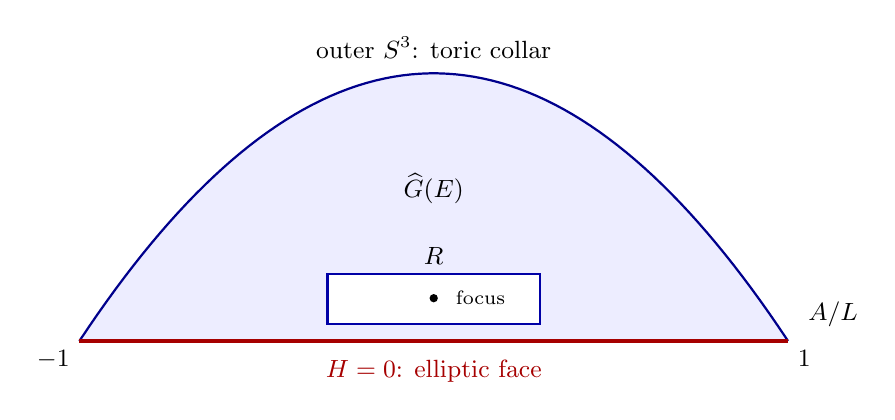
\begin{tikzpicture}[x=4.5cm,y=3.4cm,font=\small]
 \fill[blue!7] (-1,0) -- plot[domain=-1:1,samples=80] (\x,{1-\x*\x}) -- cycle;
 \draw[thick,blue!55!black] plot[domain=-1:1,samples=80] (\x,{1-\x*\x});
 \draw[very thick,red!65!black] (-1,0) -- (1,0);
 \filldraw[fill=white,draw=blue!65!black,thick] (-0.3,0.0625) rectangle (0.3,0.25);
 \fill (0,0.16) circle (1.5pt);
 \node[anchor=west,font=\scriptsize] at (0.035,0.16) {focus};
 \node[anchor=south] at (0,0.25) {$R$};
 \node at (0,0.57) {$\widehat G(E)$};
 \node[anchor=south] at (0,1.02) {outer $S^3$: toric collar};
 \node[anchor=north,text=red!65!black] at (0,-0.035) {$H=0$: elliptic face};
 \node[anchor=north east] at (-1,0) {$-1$};
 \node[anchor=north west] at (1,0) {$1$};
 \node[anchor=west] at (1.03,0.10) {$A/L$};
\end{tikzpicture}
\caption{Normal補完の商座標図．縦座標は $4\pi^2H/L^2$ で，
外側の曲線は $4\pi^2H/L^2=1-(A/L)^2$．白い長方形は固定するfocus blockの像，
淡色部分はnormal exteriorの像である．図は一つの許される寸法の例であり，
integral-affine図ではない．下辺のelliptic faceが大域化の課題として残る．}
\label{ncc:fig:completion-base}
\end{figure}

\begin{corollary}[Closed curveに沿うnormal ball全体への延長]
\label{ncc:product-completion}
定理\ref{tnc:actual-curve}のnormal-trivial symplectic curve $C'$と，
そのproduct neighborhood $C'\times D^4_\rho$を用いる．
既存のconnected-level quotient $q:C'\to\Gamma$に対して，
\[
 \widehat\Pi=(\widehat G,q):C'\times D^4_\rho
              \longrightarrow\Delta_\rho\times\Gamma
\]
は，$C'\times K_c$のfibrationを開近傍ごと保ち，outer normal collarで
標準toric normal fibrationと$q$との積になる．正則fibersはLagrangian $T^3$である．
新たな$H=0$上のwhole fibersは，$\Gamma$のregular point上では$T^2$，
trivalent vertex上では$S^1\times(S^1\vee S^1)$である．
これらはsmooth strata上でisotropicであり，Euler characteristicは零である．
既存のfocus--hyperbolic rank-zero fibersとその個数は変わらない．
\end{corollary}

\begin{proof}
Symplectic product neighborhoodの同型で定理\ref{ncc:normal-ball-completion}の構成を運ぶ．
NormalとcurveのfunctionsはPoisson可換であり，whole fibersは対応するconnected fibersの積である．
Elliptic circleとcurveのcircleまたはfigure-eightの積が表示した新fibersを与える．
それらのEuler characteristicは$\chi(S^1)=0$により零である．
Normal focus fiberとその近傍は変更していないので，focus--hyperbolic fibersは保存される．
\end{proof}

\begin{remark}[Elliptic faceは境界なしの大域化を解決しない]
\label{ncc:elliptic-face-limitation}
この補完はouter normal collarをtoric化するが，$H=0$にgenuineなelliptic base boundaryを作る．
特に$-L<A<L$かつ$\Gamma$のregular point上では，whole elliptic fiberは
normal ballの内部にあるcompact $T^2$で，base germは三次元half-spaceである．
このfiberをwhole fiberとして保ち，その近傍のfiber decompositionも保つ
compact $X_d$ から Hausdorff base への大域quotientは，このbase boundary germを取り除けない．
実際，fiberを含む開集合 $O$ をnormal ballの内部に取る．
大域写像 $p$ はcompact sourceからHausdorff targetへの写像なのでclosedであり，
$B\setminus p(X_d\setminus O)$ はそのfiberの値を含み，全逆像が $O$ に入る開近傍である．
従ってquotient germは元と同じである．
従ってboundary-freeな大域baseを得るには，このelliptic faceの近傍自体を変更するか，
whole fiber条件を変更する追加の構成が必要である．
これはnormal exteriorのfibrationの存在と，大域のboundary-free fillingとを分ける条件である．
\end{remark}

\subsection{Normal exterior の round handle と相対 CW 模型}
\label{tnc:relative-handles-section}

以下で smooth handle の存在と Lagrangian filling の存在を区別する．
$Y=\partial K_c$，$E=D^4\setminus\operatorname{int}K_c$ とし，
outer boundary $S^3=\partial D^4$ を指定する．
Round handle は Asimov \cite{asimov-round} による標準的な道具であるが，
ここで必要な分解は Hopf 商から直接構成する．

\begin{proposition}[Hopf fibers に沿う一つの round handle]
\label{tnc:normal-round-handle}
Corners を丸めた $E$ は，outer $S^3$ を incoming boundary とした
smooth cobordism として，$S^3\times[0,1]$ に
\[
 R=S^1\times D^1\times D^2,
 \qquad \partial_-R=S^1\times\partial D^1\times D^2
\]
を一つ付けて得られる．
二つの attaching solid tori は Hopf fibration $S^3\to S^2$ の
二つの fiber の tubular neighborhoods であり，
その parametrization は円束の局所自明化から取る．
特に core circles は linking number の絶対値が一の Hopf link をなす．
Framing を任意の knot framing に置き換えてよいという主張ではない．

この round handle は通常の $1$-handle と $2$-handle を一つずつに分解できる．
逆向きの cobordism，すなわち $Y$ を incoming とする表示では，
通常の $2$-handle と $3$-handle を一つずつ持つ．
\end{proposition}

\begin{proof}
補題\ref{tnc:focus-exterior-hopf}の商 $B$ は，
solid torus から open $3$-ball を除いたものなので，
outer sphere を incoming として
\[
 B=(S^2\times[0,1])\cup_{\partial D^1\times D^2}(D^1\times D^2)
\]
という smooth relative handle 表示を持つ．
$E\to B$ は principal $S^1$-bundle である．
Sphere collar 上では外側境界の Hopf bundle の積であり，
$D^1\times D^2$ 上では自明である．
従ってこの表示を円束で引き戻すと所要の round handle 表示になる．
Attaching disks の各点の fiber は outer Hopf fiber であり，
二つの core circles は Hopf link である．
円束の局所自明化が全 attaching map を指定するので，
この記述は抽象的な homotopy 型だけによるものではない．

通常の handles への分解も直接見える．
$S^1=I_0\cup I_1$ を端点で交わる二つの閉区間に分ける．
$I_0\times D^1\times D^2$ は core $D^1$，cocore $I_0\times D^2$ を持つ
$4$-dimensional $1$-handle である．
残りの $I_1\times D^1\times D^2$ は core $I_1\times D^1$，cocore $D^2$ を持ち，
\[
 (\partial I_1\times D^1\times D^2)
 \cup(I_1\times\partial D^1\times D^2)
 =\partial(I_1\times D^1)\times D^2
\]
に沿って付く $2$-handle になる．
向きを逆にした handle 表示では index $k$ は $4-k$ になる．
\end{proof}

\begin{lemma}[逆向きの唯一の $2$-handle の attaching class]
\label{tnc:reverse-handle-loop}
命題\ref{tnc:normal-round-handle}の $Y$ から $S^3$ への表示において，
唯一の $2$-handle の attaching loop は，ある $k\in\mathbb Z$ に対して
\[
 a^k b^{\pm1}\in
 \pi_1(Y)=\langle a,b,t\mid[a,b]=[a,t]=1,\ [t,b]=a\rangle
\]
を表す．Whisker と向きを選び直せば，その based class を $b$ とできる．
この一つの関係の normal closure は $a,b$ の両方を殺し，$t$ を残す．
これは attaching loop の homotopy class の主張であり，その knot isotopy class や framing の同定ではない．
\end{lemma}

\begin{proof}
$3$-handle は基本群を変えないので，$\pi_1(Y)\to\pi_1(E)$ の kernel は
唯一の $2$-handle の attaching class の normal closure である．
この class 自身は $\pi_1(E)=\langle\tau\rangle$ で消えるから，
境界写像の表により $a^k b^\ell$ と書ける．
Abelianization では $a$ は零なので，$H_1(E)$ は
$\mathbb Z b\oplus\mathbb Z t$ を関係 $\ell b=0$ で割った群となる．
既知の境界写像では $b$ が零，$t$ が $\mathbb Z$ の生成元へ写るから，
$\ell=\pm1$ でなければならない．
$tbt^{-1}=ab$ による conjugation と loop の向きの反転で $b$ に正規化できる．
$b=1$ は $a=[t,b]=1$ も含意し，残る商は $\mathbb Z t$ である．
\end{proof}

\begin{theorem}[管状補集合を保つ homotopy pushout]
\label{tnc:relative-pushout}
$C=C'$，$V_0=\overline{X_d\setminus\operatorname{int}(C\times D^4)}$ とする．
$p\in S^3$ を固定し，$i:C\to V_0$ を section $z\mapsto(z,p)$ の包含とする．
$W_0=S^1\vee S^2$ の wedge point を $*$ とすると，
$V_0$ からの構造写像を保つ homotopy equivalence
\begin{equation}\label{tnc:eq:relative-pushout}
 \mathcal V\simeq
 V_0\cup_i\bigl(C\times W_0\bigr),
 \qquad (z,*)\sim i(z),
\end{equation}
がある．右辺は homotopy pushout としても解釈できる．
また $i$ は，曲面の標準的な $1$-skeleton を潰す写像
$q:C\to S^2$ と，$e h\in\pi_2(V_0)\simeq\mathbb Z$ を表す写像
$f_e:S^2\to V_0$ の合成に homotopic である．

従って包含 $V_0\to\mathcal V$ は homotopy retraction を持つ．
その homotopy cofiber は
\begin{equation}\label{tnc:eq:relative-cofiber}
 \mathcal V/V_0\simeq
 S^1\vee\bigvee^{2g+1}S^2
 \vee\bigvee^{2g+1}S^3\vee S^4.
\end{equation}
\end{theorem}

\begin{proof}
命題\ref{tnc:focus-exterior-homotopy}の証明中の homotopy pushout 比較は，
outer sphere からの構造写像を保って
\[
 (E,S^3)\simeq(S^3\vee W_0,S^3)
\]
を与える．Cofibration の homotopy extension property を用いれば，
必要な map と homotopies を $S^3$ 上で固定して取れる
\cite[Propositions~0.18--0.19]{hatcher-bct}．
$C$ との積を取り，collar に沿う pushout
$\mathcal V=V_0\cup_{C\times S^3}(C\times E)$ に適用する．
$C\times(S^3\vee W_0)$ は $C\times S^3$ と $C\times W_0$ を
共通の $C$ に沿って貼った空間だから，pushout の結合性から
\eqref{tnc:eq:relative-pushout}を得る．

$V_0$ は simply connected なので，$i$ を曲面の $1$-skeleton 上で
定数となるように homotope できる．この homotopy は曲面全体へ延長できる．
従って変更後の $i$ は $q:C\to S^2$ を通じて分解する．
Hurewicz 同型 $\pi_2(V_0)\simeq H_2(V_0)$ の下で
$i_*[C]=e h$ だから，因子 $S^2\to V_0$ は $f_e$ の homotopy class に属する．
Homotopic attaching map への変更は $V_0$ を固定する homotopy 型を変えない．

右辺では $V_0$ 上の identity と
$C\times W_0\to C\xrightarrow{i}V_0$ を合わせれば retraction になる．
また $V_0$ を潰すと
\[
 (C\times W_0)/(C\times\{*\})
 = C_+\wedge W_0
 \simeq (S^1\vee\Sigma C)\vee(S^2\vee\Sigma^2C)
\]
である．ここで $C_+$ は disjoint basepoint を加えた空間である．
例えば $C_+\wedge S^1$ は $C\times I$ の両端を一つの点に潰した空間で，
$C$ の基点を通る区間を選ぶと $S^1\vee\Sigma C$ に分裂する．
さらに一回 suspend すれば $S^2\vee\Sigma^2C$ を得る．
曲面の $2$-cell の attaching word は commutators の積であり，
その suspension は各 $S^2$ 成分への degree が零だから null-homotopic である．
従って $\Sigma C\simeq\bigvee^{2g}S^2\vee S^3$ であり，
式\eqref{tnc:eq:relative-cofiber}が従う．
\end{proof}

\begin{proposition}[六次元の相対 handle 数と次数関係]
\label{tnc:product-relative-handles}
$W=C\times E$ とし，
$A_{\mathrm{out}}=C\times S^3$，$A_{\mathrm{in}}=C\times Y$ とする．
$W$ は $A_{\mathrm{out}}$ から，通常の smooth handles を
\[
\begin{array}{c|rrrr}
 \text{index}&1&2&3&4\\ \hline
 \text{個数}&1&2g+1&2g+1&1
\end{array}
\]
だけ付けて得られる．これらの個数は各次数の相対整数 Betti 数に等しい．
特にどの smooth relative handle 表示でも index $4$ の handle は少なくとも一つ必要である．

式\eqref{tnc:eq:relative-pushout}で $i=f_e q$ に正規化した相対 CW 模型では，
$C$ の $2$-cell と $S^1$ の $1$-cell の積から来る $3$-cell が，
次数二の equivariant 関係
\[
 e(\tau-1)h=0
\]
を与える．これは smooth attaching sphere の isotopy class や framing を決定する主張ではない．
\end{proposition}

\begin{proof}
命題\ref{tnc:normal-round-handle}による $E$ の relative Morse function は
index $1,2$ の critical points を一つずつ持つ．
$C$ との積では，これら二点に対応する critical submanifolds は $C$ である．
$C$ 上の，index $0,1,2$ の critical points がそれぞれ $1,2g,1$ 個の Morse function を用いて，
各 critical submanifold の近傍で十分小さい Morse--Bott perturbation を行う．
境界 collar 上では元の関数を保ち，critical locus の外では微分が零から離れているので，
小さい perturbation は新しい critical points を生じない．
Index は和になるため表示した個数を得る．

Pair $(E,S^3)$ の相対 homology は次数 $1,2$ でそれぞれ $\mathbb Z$，
他の次数では零である．K\"unneth 公式により
\begin{equation}\label{tnc:eq:relative-homology-out}
 H_k(W,A_{\mathrm{out}};\mathbb Z)\simeq
 \begin{cases}
  \mathbb Z,&k=1,4,\\
  \mathbb Z^{2g+1},&k=2,3,\\
  0,&\text{その他}.
 \end{cases}
\end{equation}
相対 cellular chain group の rank は同じ次数の homology rank 以上なので，
各 handle 個数はこの homological lower bound を達成している．
Excision により同じ相対群は $H_k(\mathcal V,V_0;\mathbb Z)$ でもある．

最後の関係は，正規化した $i=f_eq$ に対する product CW construction から読める．
曲面の $1$-cells は $V_0$ 内で定数であり，
それらと $S^1$ の積は $2g$ 個の新しい $2$-cells を与える．
曲面の $2$-cell と $S^1$ の積の boundary で，$S^1$ 方向の両端は
universal cover の隣接する二つの $V_0$ に入り，それぞれ $\tau e h$ と $e h$ を表す．
残る側面は曲面の commutator word に沿う．
その各 $1$-cell は正負に一回ずつ現れ，曲線方向の loops は deck group へ自明に写るので，
新しい $2$-cells に対する係数は全て零である．
従って向きを選べば境界は $e(\tau-1)h$ になる．
ここで述べているのは，$V_0$ 内部の関係を既に課した次数二の module 上の表示である．
この計算だけから，smooth handles の framed attaching maps 全体や
$4$-cell の attaching map を推定しない．
\end{proof}

\begin{corollary}[Weinstein cobordism による全体移行の障害]
\label{tnc:no-weinstein-normal-transition}
$W=C\times E$ は，$A_{\mathrm{out}}$ と $A_{\mathrm{in}}$ を二つの全境界成分として，
どちらを incoming boundary としても Weinstein cobordism にはならない．
これは任意の候補 Weinstein structure に対する位相的な障害である．
\end{corollary}

\begin{proof}
実六次元の Weinstein cobordism の Morse handles は index $3$ 以下である．
実際，Liouville vector field の stable manifolds は isotropic なので，
Morse index は複素次元以下になる
\cite[Section~1]{cieliebak-eliashberg-flexible-local}．
従って incoming boundary に対する次数 $3$ より上の相対 homology は零でなければならない．
$A_{\mathrm{out}}$ が incoming なら，式\eqref{tnc:eq:relative-homology-out}の
$H_4(W,A_{\mathrm{out}})=\mathbb Z$ がこれに反する．
逆向きでは Poincar\'e--Lefschetz duality と相対群の torsion-freeness により
\[
 H_5(W,A_{\mathrm{in}};\mathbb Z)
 \simeq H^1(W,A_{\mathrm{out}};\mathbb Z)=\mathbb Z
\]
であり，やはり不可能である．
\end{proof}

\begin{remark}[障害の範囲]
\label{tnc:relative-handles-scope}
上の否定は，二つの閉境界成分をそのまま incoming/outgoing として扱う
Weinstein cobordism に対するものである．
Boundary を切り分けて新しい側面を加える場合，
非 exact な symplectic cobordism，あるいは singular Lagrangian fibration の存在は否定しない．
特に smooth handle 表示は得られたが，それを Weinstein handles だけで実現して
normal face を埋める方法は採用できない．
また cofiber の wedge 分解から $\mathcal V$ 自体を
$V_0$ とその cofiber の wedge と同一視してはいけない．
その誤同定は $e(\tau-1)h$ の関係を失う．
\end{remark}


\begin{corollary}[曲線を切った場合の相対 homology]
\label{tnc:punctured-relative-handles}
$C^\circ$ が genus $g$，$r\ge1$ 個の境界成分を持つ compact surface なら，
\[
 H_k(C^\circ\times E,C^\circ\times S^3;\mathbb Z)
 \simeq
 \begin{cases}
  \mathbb Z,&k=1,\\
  \mathbb Z^{2g+r},&k=2,\\
  \mathbb Z^{2g+r-1},&k=3,\\
  0,&\text{その他}.
 \end{cases}
\]
従って outer boundary に対する次数 $4$ の障害は消えるが，
新しい側面 $\partial C^\circ\times E$ の接続条件が生じる．
Weinstein structure の存在をこの消滅から結論しない．
\end{corollary}
\begin{proof}
$C^\circ$ の homology は $H_0=\mathbb Z$，
$H_1=\mathbb Z^{2g+r-1}$ のみなので，
$(E,S^3)$ の相対 homology との K\"unneth 公式が表示を与える．
ここで relative subspace は $C^\circ\times S^3$ だけであり，
$\partial C^\circ\times E$ を incoming boundary に含めた計算ではない．
\end{proof}

\subsection{境界を埋める円板の非可換関係}
\label{tnc:relative-disk-extension}

境界包含の基本群写像の kernel を求めるだけでは，
各 loop を埋める円板の間に必要な関係は分からない．
ここでは normal pair の crossed module と，三次元補集合の
第二相対 homotopy group の通常の群構造を計算する．
三次元全体での全境界作用の表示，smooth handle の framing，
isotropic attaching sphere の構成までは結論しない．

\begin{theorem}[Normal pair の相対円板と二階差分]
\label{tnc:normal-relative-disk-module}
$Y\hookrightarrow E$ の relative group は abelian であり，
$\pi_1(Y)$ の作用は $\pi_1(E)=\langle\tau\rangle$ を経由する．
従って $\mathfrak R_E=\pi_2(E,Y)$ は $\Lambda$-module となる．
逆向きの唯一の $2$-handle の core に，適切な向きと whisker を与え，
その boundary が $b$ となる relative disk class $B$ を選べば
\[
 \mathfrak R_E\simeq\Lambda B
\]
とできる．$\langle a,b\rangle\simeq\mathbb Z^2$ をこの式でだけ加法的に書けば，
boundary は Laurent polynomial $f$ に対して
\[
 \partial(fB)=f(1)b+f'(1)a
\]
である．従って $\pi_2(E)$ の適当な $\Lambda$-generator
$\nu_{\mathrm{rel}}$ に関して exact sequence
\[
 0\longrightarrow\Lambda\nu_{\mathrm{rel}}
   \xrightarrow{\ \nu_{\mathrm{rel}}\mapsto(\tau-1)^2B\ }
   \Lambda B\xrightarrow{\partial}\mathbb Z a\oplus\mathbb Z b
   \longrightarrow0
\]
を得る．以下では $\pi_2(E)$ をその像と同一視する．$A=(\tau-1)B$ と置くと
\[
 \partial A=a,\qquad
 {}^tB=B+A,\qquad {}^tA=A+\nu_{\mathrm{rel}}.
\]
$\nu_{\mathrm{rel}}$ と既存の sphere generator の差は
$\pm\tau^n$ という unit の選択だけであり，marked torus の向きを
暗黙に固定し直しているわけではない．
\end{theorem}
\begin{proof}
$Y$ の universal cover は contractible である．
従って pair の homotopy 長完全列と
$\pi_1(Y)\to\pi_1(E)$ の計算により
\[
 1\longrightarrow\pi_2(E)\longrightarrow\mathfrak R_E
   \longrightarrow\langle a,b\rangle\longrightarrow1
\]
となり，kernel は crossed-module の Peiffer identity により central である．
$\widehat Y\subset\widetilde E$ を connected inverse image とすると，
$\widehat Y\cong T^2\times\mathbb R$ である．
この central extension の class は，次の証明でも詳述する
homotopy-fiber の記述により
\[
 H_2(\widehat Y;\mathbb Z)\longrightarrow
 H_2(\widetilde E;\mathbb Z)=\pi_2(E)
\]
で決まる．この写像は零である．実際，generator $F$ は
補題\ref{tnc:normal-boundary-maps}の $S^1_a\times D^2_b$ で埋まり，
その solid torus の基本群の $\pi_1(E)$ への像が零なので，
solid torus 全体が $\widetilde E$ へ持ち上がる．
$H_1(T^2;\mathbb Z)$ は free なので extension class に他の成分はない．
よって extension は abelian groups の direct product として split し，
$\mathfrak R_E$ は abelian である．

境界の kernel $\langle a,b\rangle$ の作用は，その relative lift による
inner conjugation に等しいから trivial である．従って全境界作用は
$\langle\tau\rangle$ を経由する．また
$(\widetilde E,\widehat Y)$ は $1$-connected pair である．
一般の relative Hurewicz theorem は
$\pi_1(\widehat Y)$ の作用による quotient を取って初めて成立するが
\cite[Theorem~4.37]{hatcher-bct}，ここでは今述べた作用が trivial なので
\[
 \mathfrak R_E\simeq H_2(\widetilde E,\widehat Y;\mathbb Z)
\]
を $\Lambda$-module として得る．

命題\ref{tnc:normal-round-handle}の reversed relative handle decomposition は
一つの index-$2$ handle と一つの index-$3$ handle からなる．
従って universal-cover relative cellular chain は，次数 $2,3$ に
それぞれ一つの $\Lambda$ を持ち，他の次数では零である．
上の exact sequence の quotient $\mathbb Z^2$ は
$(\tau-1)^2$ で殺されるので，$\mathfrak R_E$ の $\Lambda$-rank は一である．
もし唯一の differential $d_3:\Lambda\to\Lambda$ が非零なら，
$\Lambda$ の fraction field 上で同型となり，この rank は零になってしまう．
従って $d_3=0$ であり，$\mathfrak R_E\simeq\Lambda$ である．
補題\ref{tnc:reverse-handle-loop}により，index-$2$ handle の orientation と
whisker を選んで，その disk class $B$ の boundary を $b$ にできる．
これは relative cellular generator なので $\Lambda$-basis となる．

$\pi_1(Y)$ の relation $tbt^{-1}=ab$ から
$\partial(\tau^nB)=b+n a$ が全ての $n\in\mathbb Z$ に対して成立する．
これが $\partial(fB)=f(1)b+f'(1)a$ を与える．
その kernel は $f(1)=f'(1)=0$，すなわち
$(\tau-1)^2\Lambda$ である．$\pi_2(E)\simeq\Lambda$ の generator を
unit 倍して $\nu_{\mathrm{rel}}\mapsto(\tau-1)^2B$ とすれば，
残りの式は $A=(\tau-1)B$ から従う．
\end{proof}

\begin{remark}[Normal disk action の意味]
$a$ と $b$ は $E$ の中でともに null-homotopic であるが，
その filling disks を $t$ に沿って運ぶ操作は自明ではない．
一度の差分が $a$ の disk を作り，二度の差分が sphere generator を作る．
これは normal pair の crossed module を決定する計算であり，
円板が Lagrangian であることや，handle framing が symplectic attachment に
適合することを追加で主張しない．
\end{remark}

$\mathcal A=\partial\mathcal U=C\times Y$，
$\Gamma_C=\pi_1(C)$ とし，
\[
 M=\pi_2(\mathcal V),\qquad
 \mathfrak R=\pi_2(\mathcal V,\mathcal A).
\]
$M$ は定理\ref{tnc:equivariant-pi2}で求めた $\Lambda$-module であるが，
次の central extension ではその underlying abelian group を使う．
$h\in M$ は一つの $V_0$ の lift の正の二次元生成元とする．

\begin{theorem}[Relative disk group の central extension]
\label{tnc:relative-disk-central-extension}
境界写像によって exact sequence
\[
 1\longrightarrow M\xrightarrow{\iota}\mathfrak R
   \xrightarrow{\partial}\Gamma_C\times\mathbb Z_a\times\mathbb Z_b
   \longrightarrow1
\]
を得る．$\iota(M)$ は $\mathfrak R$ の中心に含まれる．
Surface generators $\alpha_i,\beta_i$ ($1\le i\le g$) と向きを固定し，
その相対円板による lifts を $A_i,B_i$，$a,b$ の lifts を
$\mathfrak a,\mathfrak b$ とする．符号規約を曲線の向きに合わせると，
この extension は
\[
 \prod_{i=1}^g[A_i,B_i]=\iota(eh)
\]
および $\iota(M)$ の centrality と
\[
 [\mathfrak a,\mathfrak b]=1,\qquad
 [\mathfrak a,A_i]=[\mathfrak a,B_i]
 =[\mathfrak b,A_i]=[\mathfrak b,B_i]=1
\]
を relations として表示される．ここで $M$ 自身の全加法的関係を
$\iota(m+n)=\iota(m)\iota(n)$ として含める．
この central extension は split しない．
\end{theorem}

\begin{proof}
$C$ は genus $g\ge3$ の閉曲面，$Y$ は $T^2$ の mapping torus なので，
$\mathcal A$ は aspherical である．
定理\ref{tnc:actual-complement-pi1}により
\[
 K:=\ker\bigl(\pi_1(\mathcal A)\to\pi_1(\mathcal V)\bigr)
   =\Gamma_C\times\langle a,b\rangle
   \simeq\Gamma_C\times\mathbb Z^2.
\]
$\pi_2(\mathcal A)=0$ と pair の homotopy 長完全列から，
主張した short exact sequence を得る．
相対境界 $\partial:\pi_2(\mathcal V,\mathcal A)\to\pi_1(\mathcal A)$
は fundamental crossed module である
\cite[Section~2]{brown-relative-pi2}．
Peiffer identity において $\partial\iota(m)=1$ と置けば，
$\iota(m)$ と全ての相対類との可換性が従う．

$\widehat{\mathcal A}\to\mathcal A$ を $K$ に対応する connected cover とする．
$Y$ の mapping-torus base を $\mathbb R$ に持ち上げる被覆なので
\[
 \widehat{\mathcal A}\cong C\times T^2\times\mathbb R.
\]
これは universal cover $\widetilde{\mathcal V}$ の境界の逆像である．
Relative disks とその homotopies の一意的 lift により
\[
 \pi_2(\mathcal V,\mathcal A)
   \simeq\pi_2(\widetilde{\mathcal V},\widehat{\mathcal A}).
\]

この central extension の class は
\[
 H^2(K;M)=H^2(C\times T^2;M)
   \simeq\operatorname{Hom}\bigl(H_2(C\times T^2;\mathbb Z),M\bigr)
\]
に属する．最後の同型は $H_1(C\times T^2;\mathbb Z)$ が free であることと
universal coefficient theorem による．
ここで $K$ の coefficient $M$ への作用は trivial であり，
full boundary group の作用が trivial だという意味ではない．
Central extensions の $H^2$ による分類は
\cite[Section~2]{conrad-group-extensions}を参照．

この class が，inclusion による写像
\[
 H_2(\widehat{\mathcal A};\mathbb Z)
   \longrightarrow H_2(\widetilde{\mathcal V};\mathbb Z)=M
\]
そのものであることも確認しておく．
$\widetilde{\mathcal V}$ は simply connected なので，
$H^2(\widetilde{\mathcal V};M)$ の identity に対応する class を
代表する map $p:\widetilde{\mathcal V}\to K(M,2)$ がある
\cite[Theorem~4.57]{hatcher-bct}．
$p$ は $\pi_2$ 上で identity を誘導する．
Inclusion $j:\widehat{\mathcal A}\to\widetilde{\mathcal V}$ と
$p j$ の homotopy fibers の $\pi_1$ は，homotopy 長完全列の比較により
kernel $M$ と quotient $K$ を保って同型になる．
後者は $p j$ が表す $H^2(K;M)$ の class に対応する central extension である．
実際，one-skeleton の lifts を選び，two-cell の境界を一周すると，
$p j$ のその two-cell 上の値が central な relation として現れる．
従って extension class の evaluation は上の inclusion map と一致する．

その写像を K\"unneth 分解で計算する．
$[C]\times\{*\}$ は $e h$ へ写る．
$H_1(C)\otimes H_1(T^2)$ は inclusion が
$C\times\widetilde E$ を経由し，$H_1(\widetilde E)=0$ なので零へ写る．
最後の $[T^2]=F$ も零へ写る．
これには ordinary $H_2(E)$ への消滅だけでは足りないが，
補題\ref{tnc:normal-boundary-maps}の explicit solid torus
$S^1_a\times D^2_b\subset E$ は，その $\pi_1$ が $\pi_1(E)$ で零となるため
$\widetilde E$ に持ち上がり，lift した $F$ を埋める．
ゆえに extension class は surface orientation class $u_C$ を用いて
\[
 (e h)\,\operatorname{pr}_C^*u_C
\]
である．Surface polygon の relation と全ての mixed tori に評価すれば，
上の presentation を得る．

最後に ambient hyperplane class による homomorphism
\[
 \ell:M\longrightarrow\mathbb Z,\qquad
 \ell(m)=\langle H,m\rangle
\]
は $\ell(h)=1$ を満たす．特に $e h\ne0$ なので extension class は非零であり，
extension は split しない．
\end{proof}

\begin{corollary}[Curve relation の不変性と degree の quotient]
\label{tnc:relative-disk-degree}
Curve generators を埋める相対円板を選び直しても，
$\prod_i[A_i,B_i]=\iota(e h)$ は変わらない．
さらに normal base circuit $t$ の作用との整合性は
$e(\tau-1)h=0$ を要求する．
また $\ell$ を上の homomorphism とすると，
\[
 \mathfrak R/\iota(\ker\ell)
   \simeq\pi_1(P_e)\times\mathbb Z^2,
\]
ただし $P_e\to C$ は Euler number $e$ の oriented circle bundle
（boundary orientation の規約に応じて全体の符号を固定）である．
\end{corollary}
\begin{proof}
同じ boundary loop の二つの lifts の差は central subgroup $\iota(M)$ に属する．
従って各 commutator は不変である．
$t$ は $\pi_1(\mathcal A)=\Gamma_C\times\pi_1(Y)$ の中で
curve generators と可換なので，$t$ を作用させた $A_i,B_i$ も同じ
curve generators の lifts である．左辺は変わらず，右辺は
$\iota(e\tau h)$ へ写るため $e\tau h=e h$ を得る．
最後の quotient は，central subgroup $M$ を $\ell$ によって
$\mathbb Z\langle z\rangle$ へ押し出した extension である．
その presentation は
\[
 \prod_i[A_i,B_i]=z^e,
 \qquad z\ \text{central},
\]
と独立な二つの central generators $\mathfrak a,\mathfrak b$ からなる．
Surface polygon の clutching degree $e$ による circle bundle の
fundamental group と一致する．
\end{proof}

\begin{remark}[相対円板計算の範囲]
これは boundary loops が個々に消えるという条件を，
その filling disks が満たすべき nonabelian relation へ強めたものである．
Curve relation を全て自明にする disk system は存在しない．
ただし，$t$ による各 disk lift の作用の全表示，embedded disk の選択，
smooth handle framing，Lagrangian attaching data はまだ決定していない．
また $\mathcal A$ 自体は Lagrangian ではないから，
$\mathfrak R$ 全体に symplectic area を relative homotopy invariant として
定義してはならない．Sphere subgroup $M$ 上では
$\int_m\omega=a\ell(m)$，$\langle c_1(TX_d),m\rangle=(5-d)\ell(m)$
であり，この sphere ambiguity と boundary action periods は区別する．
\end{remark}

\subsection{Marked cycleのMaslov classとclean Lagrangian disk}
\label{ncc:maslov-clean-disk-section}

\begin{lemma}[Normal regular torusのMaslov marking]
\label{ncc:normal-maslov-marking}
元の模型$G_c$のregular torus $L_{A,q}$で，$a$をinverse-phase circle，
$b$を$w-c$のpositive phaseを一周する任意のsection liftとする．
標準trivialization $\Omega=dX\wedge dY$に関するMaslov classは
\[
 \mu_L(a)=0,\qquad \mu_L(b)=2.
\]
従って$L_{A,q}$と境界でcleanに交わるsmooth embedded Lagrangian diskが
$\mathbb C^2$内に存在するなら，その境界のclass $ma+nb$は$n=0$を満たす．
さらに標準primitiveに対するStokesの定理により$mA=0$である．
特にprimitiveなessential境界classなら$A=0$かつ$\partial D=\pm a$でなければならない．
\end{lemma}

\begin{proof}
周期一のgeneratorを$V_a=2\pi(iX,-iY)$と書く．Torusのもう一つのtangent vectorを$v$とすると
\[
 \Omega(V_a,v)=2\pi i\,dw(v).
\]
$w=c+\sqrt q\,e^{i\theta}$に沿って$v$を選べば，右辺のphaseは$\theta$が一周すると一回転する．
$a$に沿っては$w$とこのphaseは変化しない．Squared phaseのwindingを取るMaslov規約により
最初の二つの式が従う．Section liftの変更は$b$へ$a$の整数倍を加えるだけなので結果は変わらない．

一般に，二つのLagrangian surfaces $L,D$がsmooth boundary curve $\gamma=\partial D$に沿って
cleanに交わるとする．その共通tangent lineを$\ell=T\gamma$とおく．
Symplectic plane bundle $\ell^\omega/\ell$内で，二つのtangent planesの商は互いに異なるreal linesである．
その相対角は$\mathbb R/\pi\mathbb Z$の一点を除いたintervalに値を取るので，
両tangent-plane loopsのsquared phasesはhomotopicである．$D$のphaseはdisk全体へ延びるため，
$\mu_L(\gamma)=0$となる．これを上の計算と合わせれば$n=0$を得る．

標準primitive
\[
 \lambda_0=\tfrac12\operatorname{Im}(\overline X\,dX+\overline Y\,dY)
\]
は$\int_a\lambda_0=A$を満たす．Lagrangian diskには$\omega_0|_D=0$なので
\[
 0=\int_D\omega_0=\int_{\partial D}\lambda_0=mA
\]
である．Primitiveなessential classで$n=0$なら$m=\pm1$であり，結論を得る．
\end{proof}

\begin{remark}
この障害は，null-homotopicなmarked loopをclean Lagrangian core diskで埋める方法への制約である．
Elliptic degenerationでcircleを潰すときのtransverse diskはsymplecticであり，この障害の対象ではない．
従って上のnormal completionと矛盾しない．また，diskがcurve方向にも動く三次元ambientの場合や，
boundaryでclean条件を失うsingular diskへの非存在をここでは主張しない．
\end{remark}

\section{Normal clutching の weighted collar と有限 isotropy}
\label{tcf:section}

閉曲線から削除した disk を戻す際、normal frame の winding を symplectic な
collar coordinates に反映させる必要がある。本節では、その exact な変換と、
同じ weighted $T^2$ action を disk 側まで保つと現れる singularity を計算する。
外側の whole focus collar は厳密に合わせられるが、それだけで自由境界のない cap は得られない。
特に一つの disk に大きい determinant winding を集中させると、
その action を保った nonelliptic な修正には高次退化が避けられない。

\subsection{Weighted action と exact な外側 collar}

標準 $\CC^3_{w,x,y}$ 上で、角度の周期を $1$、$P_z=\pi|z|^2$ とする。
$a,b\in\ZZ_{\ge0}$、$m=a+b>0$ を固定し、
\begin{equation}\label{tcf:actions}
 H=P_w+aP_x+bP_y,\qquad J=P_x-P_y
\end{equation}
と置く。これらの Hamiltonian flows は effective な $T^2$ action
\begin{equation}\label{tcf:torus-action}
 (s,t)\cdot(w,x,y)
 =\bigl(e^{2\pi is}w,e^{2\pi i(as+t)}x,e^{2\pi i(bs-t)}y\bigr)
\end{equation}
を与える。

$w\ne0$ の上で $\theta=\arg(w)/(2\pi)$ とし、
\begin{equation}\label{tcf:collar-coordinates}
 X=e^{-2\pi ia\theta}x,\qquad
 Y=e^{-2\pi ib\theta}y
\end{equation}
と定める。このとき
\begin{equation}\label{tcf:primitive}
 \lambda_{\rm std}=H\,d\theta+P_Xd\theta_X+P_Yd\theta_Y,
 \qquad
 \omega_{\rm std}=dH\wedge d\theta+\omega_X+\omega_Y.
\end{equation}
従って $(H,\theta,X,Y)$ は
$H-aP_X-bP_Y>0$ 上の exact symplectic coordinates である。
逆変換は
\[
 w=e^{2\pi i\theta}\sqrt{\frac{H-aP_X-bP_Y}{\pi}},\qquad
 x=e^{2\pi ia\theta}X,\qquad y=e^{2\pi ib\theta}Y.
\]
所定の curve action が $I=H-\beta$ と規格化される場合には、
式\eqref{tcf:primitive}の第一項は $(I+\beta)d\theta$ となる。
この closed term $\beta d\theta$ は symplectic form を変えないが、marked primitive periods には残る。

\begin{proposition}[Weighted clutching と whole product-focus collar]
\label{tcf:exact-collar}
$c>0$、$j_*>0$、$0<q_-<c^2<q_+$ を固定し、
\[
 \mathcal N=\{(X,Y): |P_X-P_Y|\le j_*,\quad
                   q_-\le |XY-c|^2\le q_+\}
\]
を compact normal focus block とする。
\begin{equation}\label{tcf:normal-bound}
 M=\sqrt{j_*^2+4\pi^2(c+\sqrt{q_+})^2}
\end{equation}
とおけば、$\mathcal N$ 上で $P_X+P_Y\le M$ である。
$t_0>0$ と $h_-<h_+$ が
\begin{equation}\label{tcf:collar-bound}
 h_->t_0+\max(a,b)M
\end{equation}
を満たすとき、式\eqref{tcf:collar-coordinates}の逆変換は
$[h_-,h_+]\times S^1\times\mathcal N$ の開近傍を $P_w>t_0$ へ symplectic に埋め込む。
これは product focus fibration
\[
 (H,P_X-P_Y,|XY-c|^2)
\]
の whole fibers を保つ。
\end{proposition}

\begin{proof}
Normal block の compactness と radius formula は第\ref{mft:section}節と同じである。
$z=XY$ と書くと
\[
 P_X+P_Y=\sqrt{(P_X-P_Y)^2+4\pi^2|z|^2}
       \le\sqrt{j_*^2+4\pi^2(c+\sqrt{q_+})^2}=M.
\]
従って $P_w=H-aP_X-bP_Y>t_0$ が一様に成立し、逆変換の square root は正である。
Primitive の恒等式\eqref{tcf:primitive}が symplectic 性を示す。
Normal actions と product focus integral を文字通り保持するので、compact whole fibers も保つ。
\end{proof}

Disk の正向き boundary parameter を $\theta$ とし、normal frames が
$e_1^{\circ}=e_1^D e^{2\pi ia\theta}$、
$e_2^{\circ}=e_2^D e^{2\pi ib\theta}$ と関係する場合、
disk coordinates と punctured-side coordinates はちょうど
$x=e^{2\pi ia\theta}X$、$y=e^{2\pi ib\theta}Y$ と変換する。
従って mixed coefficient の winding は disk frame で $-m$ である。
これは degree $(a,b)$ の normal clutching を実現する exact collar model である。
ただし、任意に既定の actual embeddings の higher jets がこの模型と一致すると主張していない。
Compatible collars を選び、relative Moser により actual に移すときの局所入力である。

\subsection{外側 integral の smooth extension}

正の smooth function $\eta:[0,\infty)\to(0,\infty)$ を、
ある $0<t_1<t_0$ に対し
\[
 \eta(t)=\eta_0>0\quad(0\le t\le t_1),\qquad
 \eta(t)=\left(\frac{\pi}{t}\right)^{m/2}\quad(t\ge t_0)
\]
となるよう選ぶ。$m$ が奇数でも、第二式は $t\ge t_0>0$ 上だけの条件なので
零点での smoothness に問題はない。
\begin{equation}\label{tcf:normalized-W}
 W_\eta=\eta(P_w)\overline w^{\,m}xy,
 \qquad Q_\eta=|W_\eta-c|^2
\end{equation}
と置く。

\begin{proposition}[境界では厳密に product となる commuting extension]
\label{tcf:extension}
$(H,J,Q_\eta)$ は標準 $\CC^3$ 全体の smooth commuting triple である。
$P_w\ge t_0$ では
\[
 W_\eta=e^{-2\pi im\theta}xy=XY,
 \qquad Q_\eta=|XY-c|^2
\]
となり、命題\ref{tcf:exact-collar}の whole collar と integral values が厳密に一致する。
$a,b\ge0$、$m>0$ の下で、$H$ と $J$ を compact intervals に制限した領域は compact である。
従って、この triple の正則 compact connected fibers は Lagrangian $T^3$ である。
\end{proposition}

\begin{proof}
$W_\eta$ の $H$-weight は $-m+a+b=0$、$J$-weight は $1-1=0$ であり、
$P_w$ も invariant である。従って三つの関数は Poisson commute する。
$\eta$ は零点近傍で定数なので、$W_\eta$ はそこで polynomial の定数倍であり smooth である。
$P_w\ge t_0$ での等式は $|w|^m=(P_w/\pi)^{m/2}$ の代入で従う。

$H=h,J=j$ 上では
\begin{equation}\label{tcf:reduced-radii}
 P_x=\frac{h-P_w+bj}{m},\qquad
 P_y=\frac{h-P_w-aj}{m}.
\end{equation}
また $P_w\ge0$ と $a,b\ge0$ より $0\le P_w\le h$ である。
従って $h,j$ が bounded なら三つの radii は bounded であり、closed condition から compactness が従う。
正則 connected fiber は三つの commuting Hamiltonian vector fields の orbit であり、
それらは compact fiber 上で complete である。
従って fiber は $\RR^3/\Lambda$ で、compactness と正則性から $\Lambda$ は full lattice である。
\end{proof}

この proposition は integrals の smooth extension と、compact な regular whole fibers を与える。
指定した outer collar だけを境界に持つ cap を与えるものではない。
例えば全ての connected components を取った $H=h_+$ の level には、
$P_w$ の小さい別の成分が含まれ得る。
それらを geometric な normal-radius cutoff で切れば、一般には whole fibers を切断してしまう。
Connected components の選択、他の faces、既存 assembly との非交差は別に扱う必要がある。
局所的には $H=H_0$ の外側 $H>H_0$ と内側 $H<H_0$ を向かい合わせられるが、
この coorientation の一致だけから completion は従わない。

\subsection{中心 orbit の有限 isotropy と singularity の次数}

\begin{theorem}[Weighted center の局所分類]\label{tcf:center-classification}
$p=(0,x_0,y_0)$、$x_0y_0\ne0$ とする。
式\eqref{tcf:torus-action}の orbit は次元2で、isotropy group は $\ZZ/m$ である。
その symplectic slice は $w$-plane であり、generator は
$w\mapsto e^{2\pi i/m}w$ と作用する。

式\eqref{tcf:normalized-W}の triple について、次が成り立つ。
\begin{enumerate}
 \item $m=1$ なら $p$ は rank three の正則点である。
 \item $m=2$ なら $p$ は nondegenerate rank-two hyperbolic 点である。
       Isotropy は $\ZZ/2$ であり、transverse stable line と unstable line の
       それぞれの二つの半直線が orbit に沿って交換される。
 \item $m>2$ なら $p$ は rank-two degenerate 点であり、reduced third integral の
       最初の非零項の次数は $m$ である。
       $Q_\eta=c^2$ の transverse level は $2m$ 本の半枝を持つ。
\end{enumerate}
\end{theorem}

\begin{proof}
$p$ の isotropy equations は
$as+t\in\ZZ$、$bs-t\in\ZZ$ であり、従って $ms\in\ZZ$ である。
$(s,t)=(1/m,-a/m)$ が generator で、$w$-plane には原始 $m$ 乗根で作用する。
Moment weights の matrix
\[
 \begin{pmatrix}a&b\\1&-1\end{pmatrix}
\]
の determinant は $-m\ne0$ なので、$dH,dJ$ は $p$ で独立である。
Moment level の接空間を orbit tangent space で割った symplectic slice は
標準 $w$-plane と同一視できる。

$H,J$ を固定し、$x,y$ の phases を局所的に固定して
式\eqref{tcf:reduced-radii}に従って radii を調整する。
この transverse slice 上では
\begin{equation}\label{tcf:leading-term}
 Q_\eta-c^2=-2c\,\Re\bigl(K\overline w^{\,m}\bigr)
             +O(|w|^{m+2})+O(|w|^{2m}),
 \qquad K=\eta_0x_0y_0\ne0.
\end{equation}
$m=1$ では linear term が非零なので、$dQ_\eta$ は $dH,dJ$ と独立である。
$m=2$ では quadratic part が非退化かつ indefinite であり、hyperbolic 型になる。
Isotropy generator はこの場合 $w\mapsto-w$ なので、stable/unstable の各線上で
半直線の交換が生じる。
$m>2$ では transverse Hessian が零であり、次数 $m$ の項が非零なので退化する。

半枝の数も直接分かる。
この slice では $W_\eta=A(|w|^2)\overline w^m$ と書け、$A(0)\ne0$ である。
その phase は定数で、絶対値は正の smooth radial function である。
$w=re^{i\varphi}$、$r>0$ について $Q_\eta=c^2$ は
\[
 \cos(m\varphi-\arg A(0))=\frac{|A(r^2)|r^m}{2c}
\]
となる。$r$ が十分小さいとき、$r=0$ における $2m$ 個の単純な角度解から
それぞれ一つの半枝が生じる。
\end{proof}

$m=2$ の twisting は、単なる $T^2$ と untwisted figure-eight の積という記述には含まれない。
有限 isotropy と reverse hyperbolic orbit は fractional monodromy の文献にも現れる。
例えば Broer--Efstathiou--Lukina \cite[Section 2.1, Remark 2]{bel-fractional-tcf} は
$\ZZ/2$ isotropy を持つ curled-torus family を扱い、高次 resonances とは区別している。
本節では局所 slice の型を計算しただけであり、同論文の global hypotheses を
検証したり、本模型の fractional monodromy を算出したりしたわけではない。

\begin{proposition}[大きい isotropy を保つ nonelliptic repair の障害]
\label{tcf:invariant-repair}
$m>2$ とし、$p=(0,x_0,y_0)$、$x_0y_0\ne0$ の orbit 全体を含む
$T^2$-invariant neighborhood で
$H,J$ と Poisson commute する任意の smooth real function $G$ を取る。
この点で $(H,J,G)$ が nondegenerate corank one なら、その型は elliptic である。
従って $H,J$ とその orbit を保って nonelliptic な fibration を求める場合、
その orbit における degeneracy を解消することはできない。
\end{proposition}

\begin{proof}
$H,J$ の flows は periodic なので、Poisson commutativity は $T^2$ invariance を意味する。
従って $G$ の reduced germ は slice の rotation $w\mapsto e^{2\pi i/m}w$ に invariant である。
この rotation は非自明なので invariant linear form は零であり、reduced germ は原点で critical である。
$m>2$ では rotation angle は $0,\pi$ のいずれでもなく、invariant な実 symmetric quadratic form は
$\lambda|w|^2$ に限られる。これは、rotation matrix $R$ に対して
$R^TBR=B$ を満たす symmetric matrix $B$ が scalar matrix になることから従う。
$\lambda\ne0$ なら definite なので elliptic、$\lambda=0$ なら Hessian が退化する。
Moment directions の linear terms は $G$ から $H,J$ の linear combination を引いて除けるので、
この reduced Hessian が corank-one classification を与える。
\end{proof}

\subsection{Clutching を分散するための条件}

平面切断曲線の二つの normal lines の degree はそれぞれ $d$ である。
一つの disk に winding $(d,d)$ を集中させると、上の模型は $m=2d$ となる。
$d\ge6$ では、中心の generic orbit に $\ZZ/(2d)$ isotropy と $4d$ 本の transverse 半枝が現れ、
命題\ref{tcf:invariant-repair}により同じ action を保つ nondegenerate hyperbolic repair は存在しない。
Radial normalization は outer focus collar を厳密に保つが、この結論を変えない。

一方、winding を複数の holes に分ければ、その局所次数を小さくできる。
例えば $d$ 個の holes で $(a_i,b_i)=(1,1)$ とすれば全て $m_i=2$ となり、
中心の generic orbits は nondegenerate hyperbolic 型になる。
$2d$ 個の holes に、$(1,0)$ と $(0,1)$ をそれぞれ $d$ 個ずつ配れば、
全て $m_i=1$ となり、その中心の generic orbits は正則になる。
これは frame の degree と局所型に関する互換性であり、全ての caps が接続されたという結論ではない。

この weighted design の中で、$r$ 個の holes に全 determinant winding を配り、
全て $0<|m_i|\le2$ とするなら
\[
 2d=\left|\sum_i m_i\right|\le\sum_i|m_i|\le2r,
 \qquad r\ge d.
\]
さらに中心の generic orbit の isotropy を全て trivial にする $|m_i|=1$ を要求するなら
$r\ge2d$ が必要である。
この下界は、この指定された weighted collar construction に関するものであり、
任意の Lagrangian fibration の punctures 数に対する下界ではない。
また、本節で保持した曲線は degree $d$ の平面切断曲線である。
別の symplectic curve を選び、その symplectic normal bundle を trivial にする戦略には、
この degree $2d$ の clutching 条件を適用してはいけない。

最後に、$w=x=y=0$ では $dH=dJ=dQ_\eta=0$ で、$Q_\eta-c^2$ の最低次数は $m+2\ge3$ である。
従って原点の quadratic parts は三自由度の nondegenerate Cartan を作らず、
原点は依然として退化している。
中心の generic orbit を $m=1$ または $2$ に改善しても、原点、normal faces、
whole-fiber component の選択、および actual assembly の非交差を含む cap completion は残る。

\section{Symplectic scale と focus の return invariant}
\label{rs:section}

Moving collar では reduced form と reduced foliation を同時に輸送する。
その際に、compact focus fiber の return data を単に一定と置いてはならない。
本節では、比例する symplectic forms に対する正確な変換則を記録する。

\begin{proposition}[正則化 action の scale 変換]
\label{rs:scaling}
Compact simple focus--focus fibration の向き、vanishing cycle、補周期、
および logarithm の枝を固定する。
$(U,\omega)$ に対する Eliasson base coordinate を $c=q_1+\sqrt{-1}q_2$ とし、
action を
\[
 \mathcal A(c)=\mathcal A_0-\operatorname{Re}(c\log c-c)+S(c),
 \qquad S(0)=0
\]
と書く。
同じ fiber decomposition を持つ $(U,r\omega)$, $r>0$ に対し、
scaled primitive と induced marking を用いる。
ここで $q_2$ は period $2\pi$ の circle flow を生成する標準 Eliasson quadratic であり、
period-one action 自体とは $J=2\pi q_2$ の関係にある。
Eliasson coordinate を $c_r=rc$ と取れば、正則化 action は
\begin{equation}\label{rs:scale-law}
 S_r(c_r)=rS(c_r/r)+(\log r)\operatorname{Re}c_r
\end{equation}
となる。
特に $S$ の $q_1$ の一次係数は $\log r$ だけ変わり、
$q_2$ の一次係数は変わらない。
次数 $k\ge2$ の各係数には $r^{1-k}$ が掛かる。
\end{proposition}

\begin{proof}
正則化公式は \cite[Proposition 3.1, Remark 3.2]{vungoc-local} による。
点近傍で $\omega=\sum dx_i\wedge d\xi_i$ とすると、
$\sqrt r\,x_i,\sqrt r\,\xi_i$ は $r\omega$ の Darboux coordinates である。
標準 focus quadratics は同時に $r$ 倍されるので、$c_r=rc$ と取れる。
Primitive とその cycle integrals も $r$ 倍されるから
\[
 \mathcal A_r(c_r)=r\mathcal A(c_r/r),\qquad
 \mathcal A_{r,0}=r\mathcal A_0.
\]
一つの logarithm の枝に対して $\log(c_r/r)=\log c_r-\log r$ である。
従って
\begin{align*}
 \mathcal A_r(c_r)-\mathcal A_{r,0}
 &=-\operatorname{Re}(c_r\log c_r-c_r)
   +(\log r)\operatorname{Re}c_r+rS(c_r/r).
\end{align*}
これを正則化 action の定義と比較して式\eqref{rs:scale-law}を得る。
係数の変換則は Taylor 展開から直ちに従う。
\end{proof}

\begin{corollary}[Moving collar で要求される return data]
\label{rs:collar}
第\ref{mc:main}節の一法線方向の collar で
$r(\mu)=1-\mu/w>0$ とする。
構成された moving reduced fibration の focus invariant は、
その構成が与える marking と scaled Eliasson coordinates において
\[
 S_\mu(c)=r(\mu)S_0(c/r(\mu))+
              \log r(\mu)\operatorname{Re}c
\]
を満たす。
従って、別に指定した端の fibration と照合する際には、
Hessian のほかにこの return data の変化も照合する必要がある。
\end{corollary}

\begin{proof}
Strict Moser 同定後の reduced symplectic form は
$r(\mu)\omega$、その fiber decomposition は $p_0$ のものになる。
命題\ref{rs:scaling}を適用する。
\end{proof}

\begin{remark}[Marking と primitive の区別]
式\eqref{rs:scale-law}は向きと cycle marking を固定した式である。
補周期に vanishing cycle を加える変更や logarithm の枝の変更には、
通常の integral-affine ambiguity がある。
また $\mathcal A_0$ は primitive を固定した exact comparison の情報であり、
$S$ の定義では差し引かれる。
第\ref{ae:section}節の nodal action constant の不一致と、
本節の正則化 Taylor invariant の変化を同一視しない。

固定した向きと marking の下で $r\ne1$ なら、$S_r$ と $S$ は
$q_1$ の一次係数ですでに異なる。
これは第\ref{lc:liouville-focus}節の固定 foliation に対する Liouville 障害と整合し、
同時に moving collar が必要な変化をどのように担うかを示している。
\end{remark}


\section{Trivial-normal block の外側へ}
\label{lc:next}

第\ref{tnc:section}節により、任意の所定 $X_d$ に、閉曲線全体を含み negative Euler fibers を持つ
actual block ができた。第\ref{ncc:section}節でそのnormal ball全体への補完も得た．
次の中心課題は，そのelliptic faceの処理と $V_0$ への接続である．

\begin{enumerate}
\item 構成済みのtoric outer collarに適合する $V_0$ 側の領域をactualに作る．
同時に，境界のないbaseを得るには $H=0$ のelliptic fiberの近傍自体を変更する必要がある．
Whole torusとhyperbolic fibers，boundary coorientation，primitive periodsを照合する．
新しい $C'$ の normal bundle は trivial なので、旧 generic plane section の degree $2d$ の障害は適用しない。
一方、全域へ同じ非零 periodic generator を延長することは第\ref{gc:section}節によりできない。
閉曲線全体の移行をWeinstein handlesだけで構成する方法は
系\ref{tnc:no-weinstein-normal-transition}により排除される．
曲線を切った場合は相対 $H_4$ が消えるが，新しい側面の接続を別に構成する必要がある．
\item 新しい graph の cycles を nice global base 内で縮め、circle-valued label を変更する領域を作る。
六次では構成済み block の Euler 数は $-4$、compact complement は $-512$ である。
この値を特異 fibers の個数と同一視せず、complement の全層と接続を構成する。
\item 元の generic plane section を保持する方式では、第\ref{fnc:section}節の intrinsic obstruction と
第\ref{fhr:section}節の boundary winding を守る。
Weighted collars は $m=1,2$ なら generic center の高次退化を避けられるが、
第\ref{tcf:section}節の原点と full cap、whole-fiber components の選択は未処理である。
\item 旧48 regular ports の接続は独立の相対課題として保持する。
Natural pair の面積下界、$\delta$ pair の同一 tube 内での全 genus 障害、
membrane/focus collar の action offsets と非交差条件を無条件には外さない。
\end{enumerate}

新しい closed trivial-normal block、generic plane section の punctured blocks、旧 cap assembly は
別の fibration choices であり、それらの fiber counts を加算していない。
全体の actual coverage、Hausdorff quotient、connected fibers と自由境界の消去は未証明である。
15本の検算は本文の算術と局所式を補助し、存在証明の代用とはしない。

\begin{thebibliography}{99}
\bibitem{auroux-local}
D. Auroux,
\emph{Mirror symmetry and T-duality in the complement of an anticanonical divisor},
J. G\"okova Geom. Topol. GGT \textbf{1} (2007), 51--91.
\url{https://arxiv.org/abs/0706.3207}.
Section 5.1, Proposition 5.2 の nodal model を参照。

\bibitem{cds-local}
A. Cannas da Silva,
\emph{Lectures on Symplectic Geometry}, Lecture Notes in Mathematics 1764, Springer, 2001;
revised January 2006.
\url{https://people.math.ethz.ch/~acannas/Papers/lsg.pdf}.
Sections 7.3, 9.2 の relative Moser と symplectic neighborhood theorem。

\bibitem{vungoc-local}
S. V\~u Ng\d{o}c,
\emph{On semi-global invariants for focus-focus singularities},
Topology \textbf{42} (2003), 365--380.
\url{https://arxiv.org/abs/math/0208245}.
Theorem 2.1、Proposition 3.1、Remark 3.2。

\bibitem{vw-local}
S. V\~u Ng\d{o}c and C. Wacheux,
\emph{Smooth normal forms for integrable Hamiltonian systems near a focus-focus singularity},
Acta Math. Vietnam. \textbf{38} (2013), 107--122.
\url{https://arxiv.org/abs/1103.3282}.
Theorems 1.2--1.4 は点近傍の smooth normal form とその automorphisms を扱う。

\bibitem{miranda-local}
E. Miranda and N. T. Zung,
\emph{Equivariant normal form for nondegenerate singular orbits of integrable Hamiltonian systems},
Ann. Sci. \'Ecole Norm. Sup. (4) \textbf{37} (2004), 819--839.
\url{https://arxiv.org/abs/math/0302287}.
Theorem 2.1 の orbit 近傍の normal form と、Section 2.3 の linear focus automorphism factor を参照。

\bibitem{auroux-blowup}
D. Auroux,
\emph{Special Lagrangian fibrations, wall-crossing, and mirror symmetry},
arXiv:0902.1595.
\url{https://arxiv.org/abs/0902.1595}.
Sections 3.1.2, 3.3.1 の blow-up model と torus-invariant model。

\bibitem{gross-toric}
M. Gross,
\emph{Examples of Special Lagrangian Fibrations},
arXiv:math/0012002.
\url{https://arxiv.org/abs/math/0012002}.
Sections 1--2 の Hamiltonian reduction と toric constructions。

\bibitem{cbm-conifold}
R. Casta\~no-Bernard and D. Matessi,
\emph{Conifold transitions via affine geometry and mirror symmetry},
Geometry \& Topology \textbf{18} (2014), 1769--1863.
\url{https://msp.org/gt/2014/18-3/gt-v18-n3-p12-p.pdf}.
Sections 3.4, 5.1 の explicit positive fibrations。

\bibitem{evans-gompf}
J. D. Evans,
\emph{Symplectic mapping class groups of some Stein and rational surfaces},
J. Symplectic Geom. \textbf{9} (2011), 45--82.
\url{https://arxiv.org/abs/0909.5622}.
Version 4, Section 5.2.1, Lemma 27 の局所 Gompf isotopy。

\bibitem{cg-at-blowup}
P. Chakravarthy and Y. Groman,
\emph{Almost toric fibrations on symplectic blow ups},
arXiv:2510.00994, version 1 (2025).
\url{https://arxiv.org/abs/2510.00994}.
Theorem 1.1, Definitions 2.2--2.3 の相対領域と divisor compatibility。

\bibitem{loi-zuddas-local}
A. Loi and F. Zuddas,
\emph{Symplectic maps of complex domains into complex space forms},
arXiv:0803.3532v1.
\url{https://arxiv.org/abs/0803.3532}.
Theorem 1.1 and the explicit radial maps in Section 2.


\bibitem{lerman-cut-local}
E. Lerman,
\emph{Symplectic cuts},
Math. Res. Lett. \textbf{2} (1995), 247--258.
\url{https://doi.org/10.4310/MRL.1995.v2.n3.a2}.
Section 1.1, Remarks 1.2 and 1.6 の cut と可換な Hamiltonian actions。

\bibitem{zung-focus-cf}
N. T. Zung,
\emph{A note on focus-focus singularities},
Differential Geometry and its Applications \textbf{7} (1997), 123--130.
\url{https://arxiv.org/abs/math/0110147}.
Section 3, Lemma 1 and Corollary 1 の focus monodromy。

\bibitem{efstathiou-martynchuk-cf}
K. Efstathiou and N. Martynchuk,
\emph{Monodromy of Hamiltonian systems with complexity 1 torus actions},
Journal of Geometry and Physics \textbf{115} (2017), 104--115.
\url{https://doi.org/10.1016/j.geomphys.2016.05.014}.
Theorems 3.2 and 3.15 の curvature と monodromy の関係。

\bibitem{cho-shin-maslov}
C.-H. Cho and H.-S. Shin,
\emph{Chern--Weil Maslov index and its orbifold analogue},
arXiv:1202.0556 (2012).
\url{https://arxiv.org/abs/1202.0556}.
Sections 2.3--2.4, Example 2.10 and Theorem 3.1 の符号と $2c_1$ の規約。


\bibitem{mcduff-uniruled-gc}
D. McDuff,
\emph{Hamiltonian $S^1$-manifolds are uniruled},
Duke Math. J. \textbf{146} (2009), 449--507.
\url{https://arxiv.org/abs/0706.0675}.
Corollary 1.2. 本文では負の単調性に必要な場合を orbit sphere から直接証明する。

\bibitem{gadbled-weights-gc}
A. Gadbled,
\emph{Families of monotone symplectic manifolds constructed via symplectic cut and their Lagrangian submanifolds},
Algebr. Geom. Topol. \textbf{11} (2011), 2319--2368.
\url{https://arxiv.org/abs/1001.2325}.
Appendix A.2 の equivariant clutching と weight sums。

\bibitem{achinger-lefschetz-gc}
P. Achinger,
\emph{Fundamental groups in algebraic geometry},
lecture notes, 19 March 2025.
\url{https://achinger.impan.pl/pi1/notes.pdf}.
Section 2.3, Corollary 2.3.4 の smooth complete intersections の単連結性。


\bibitem{circle-morse-ncb}
K. A. de Rezende, G. G. E. Ledesma, O. Manzoli Neto and G. M. Vago,
\emph{Lyapunov graphs for circle valued functions},
Topology Appl. \textbf{245} (2018), 62--91.
\url{https://doi.org/10.1016/j.topol.2018.06.008}.
Theorem 5.5, Lemma 5.7 and Theorem 5.9 の circle-valued Morse functions と graph。

\bibitem{hatcher-bct}
A. Hatcher,
\emph{Algebraic Topology}, Cambridge University Press (2002).
\url{https://pi.math.cornell.edu/~hatcher/AT/AT.pdf}.
Section 1.3 の universal covering と lifting criterion，
Propositions 0.18--0.19 の homotopy pushout，
Theorems 4.32, 4.37, 4.41, 4.57 と Example 4.45 の
Hurewicz theorem，relative Hurewiczの基本群作用によるquotient，
homotopy長完全列，cohomologyの $K(G,n)$ 表現，Hopf bundle。


\bibitem{bel-fractional-tcf}
H. Broer, K. Efstathiou and O. Lukina,
\emph{A geometric fractional monodromy theorem},
Discrete Contin. Dyn. Syst. Ser. S \textbf{3} (2010), 517--532.
\url{https://doi.org/10.3934/dcdss.2010.3.517}.
Section 2.1, Remark 2 の $\mathbb Z/2$ isotropy と reverse hyperbolic 型。
本稿の weighted model に対する global fractional monodromy は主張しない。


\bibitem{randal-williams-hypersurface}
O. Randal-Williams,
\emph{Monodromy and mapping class groups of 3-dimensional hypersurfaces},
Math. Ann. \textbf{391} (2025), 1965--2003.
\url{https://doi.org/10.1007/s00208-024-02951-4}.
Section 2.1: smooth degree-$d$ threefold hypersurface の整数cohomology、
$H^3$ の自由性およびChern類からのEuler数．


\bibitem{akbulut-double-fishtail}
S. Akbulut,
\emph{Double knot surgeries to $S^4$ and $S^2\times S^2$},
arXiv:1103.3137v2 (2011).
\url{https://arxiv.org/abs/1103.3137}.
Introduction and Figure 1: $S^4$ の二つの fishtails への既知の分解を記述する．
本稿の actual 埋込みとの微分同相や symplectic 同一視は仮定しない．

\bibitem{asimov-round}
D. Asimov,
\emph{Round handles and non-singular Morse--Smale flows},
Ann. of Math. (2) \textbf{102} (1975), no.~1, 41--54.
\url{https://doi.org/10.2307/1970972}.
Round handleの標準概念を参照．本稿で用いる分解はHopf商から直接証明する．

\bibitem{cieliebak-eliashberg-flexible-local}
K. Cieliebak and Y. Eliashberg,
\emph{Flexible Weinstein manifolds}, arXiv:1305.1635 (2013).
\url{https://arxiv.org/abs/1305.1635}.
Section 1.1, pp.~2--3 の Weinstein cobordism とisotropic stable manifoldsによるindex制限．

\bibitem{brown-relative-pi2}
R. Brown,
\emph{On the second relative homotopy group of an adjunction space:
an exposition of a theorem of J.~H.~C. Whitehead},
J. London Math. Soc. (2) \textbf{22} (1980), 146--152.
\url{https://doi.org/10.1112/jlms/s2-22.1.146}.
Author PDF: \url{https://www.groupoids.org.uk/pdffiles/whiteheadthm.pdf}.
Section 2 の relative crossed module と Peiffer identity．

\bibitem{conrad-group-extensions}
B. Conrad,
\emph{Math 210B. Group cohomology and group extensions},
course handout, Stanford University.
\url{https://math.stanford.edu/~conrad/210BPage/handouts/gpext.pdf}.
Section 2 の $H^2$ によるcentral extensionの分類．

\bibitem{aak}
M. Abouzaid, D. Auroux and L. Katzarkov,
\emph{Lagrangian fibrations on blowups of toric varieties and mirror symmetry for hypersurfaces},
Publ. Math. IHES \textbf{123} (2016), 199--282.
\url{https://arxiv.org/abs/1205.0053}.
\bibitem{em}
J. D. Evans and M. Mauri,
\emph{Constructing local models for Lagrangian torus fibrations},
Ann. H. Lebesgue \textbf{4} (2021), 537--570.
\url{https://arxiv.org/abs/1905.09229}.
\bibitem{symington}
M. Symington,
\emph{Four dimensions from two in symplectic topology},
Topology and Geometry of Manifolds, Proc. Sympos. Pure Math. \textbf{71} (2003), 153--208.
\url{https://arxiv.org/abs/math/0210033}.
Sections 4.2, 8.1; Section 6.1, Lemma 6.3 and Theorem 6.5 の nodal trade．
\end{thebibliography}
\end{document}
